% concatenated from kcut_comb.tex
\documentclass[12pt, a4paper]{article}%\usepackage{CJK}
\usepackage{amsmath,amssymb,amsthm,amsfonts,latexsym,graphicx,subfigure}
%\usepackage[dvips]{color}
\usepackage[all,import]{xy}
\usepackage[numbers,sort&compress]{natbib}
\usepackage{indentfirst}
\usepackage{fancyhdr}
\usepackage{bbm}
\usepackage{enumerate,tikz}
\usepackage{caption}
\usepackage{accents,cases}
\usepackage{color,tikz}
\usetikzlibrary{matrix}
%\usepackage{algorithm}
%\usepackage{algorithmic}
\usepackage{multirow}
\usepackage[normalem]{ulem}
\useunder{\uline}{\ul}{}
\usepackage{hyperref}
\usepackage{tabularx,booktabs}
\usepackage{caption}
\usepackage{adjustbox}
\usepackage{blindtext}
\usepackage{etex}
\usepackage{amsmath}
\usepackage{amsfonts}
\usepackage{accents,cases}
\usepackage{algorithm} 
\usepackage{algorithmicx}
\usepackage{algpseudocode} 
\usepackage{graphicx} 
\usepackage{epstopdf}
\usepackage{amscd}
\usepackage{amsthm}
\usepackage{amssymb}
\usepackage{bm}
\usepackage{latexsym,float}
\usepackage{makecell}
\usepackage{multicol, multirow}
\usepackage[figuresright]{rotating}
\usepackage{longtable}
\usepackage{booktabs}
\usepackage{lscape}
\usepackage{hyperref}
\usepackage{tikz}
\usetikzlibrary{shapes,arrows}

%\usepackage{pstricks}
%\usepackage{pst-node}
%\usepackage{pst-blur}

\usepackage{graphics}
\usepackage{array}
\usepackage{enumerate}
%\usepackage{dsfont}
\usepackage{color,tikz}
\usetikzlibrary{calc,intersections}

\usepackage{algorithm,algpseudocode,float}
\usepackage{lipsum}

\makeatletter
\newenvironment{breakablealgorithm}
{% \begin{breakablealgorithm}
		\begin{center}
			\refstepcounter{algorithm}% New algorithm
			\hrule height.8pt depth0pt \kern2pt% \@fs@pre for \@fs@ruled
			\renewcommand{\caption}[2][\relax]{% Make a new \caption
				{\raggedright\textbf{\ALG@name~\thealgorithm} ##2\par}%
				\ifx\relax##1\relax % #1 is \relax
				\addcontentsline{loa}{algorithm}{\protect\numberline{\thealgorithm}##2}%
				\else % #1 is not \relax
				\addcontentsline{loa}{algorithm}{\protect\numberline{\thealgorithm}##1}%
				\fi
				\kern2pt\hrule\kern2pt
			}
		}{% \end{breakablealgorithm}
		\kern2pt\hrule\relax% \@fs@post for \@fs@ruled
	\end{center}
}
\makeatother

\usetikzlibrary{arrows,chains,matrix,positioning,scopes}
\makeatletter
\tikzset{join/.code=\tikzset{after node path={%
			\ifx\tikzchainprevious\pgfutil@empty\else(\tikzchainprevious)%
			edge[every join]#1(\tikzchaincurrent)\fi}}}
\makeatother
%
\tikzset{>=stealth',every on chain/.append style={join},
	every join/.style={->}}
\tikzstyle{labeled}=[execute at begin node=$\scriptstyle,
execute at end node=$]
\usepackage{wasysym}
\usepackage{hyperref}
\usepackage{pdfsync}
\usepackage{comment}
\usepackage[all]{xy}

\allowdisplaybreaks[4]

\usepackage{tikz-cd}
\usetikzlibrary{matrix, calc, arrows}

\DeclareMathOperator{\coker}{coker}

%\usepackage[figuresright]{rotating}

\usepackage{array}
\newcommand{\PreserveBackslash}[1]{\let\temp=\\#1\let\\=\temp}
\newcolumntype{C}[1]{>{\PreserveBackslash\centering}p{#1}}
\newcolumntype{R}[1]{>{\PreserveBackslash\raggedleft}p{#1}}
\newcolumntype{L}[1]{>{\PreserveBackslash\raggedright}p{#1}}


\setlength{\textheight}{234mm} \setlength{\textwidth}{168mm}
\setlength{\oddsidemargin}{-5mm} \setlength{\evensidemargin}{0mm}
\setlength{\topmargin}{-10mm}
\renewcommand{\arraystretch}{1.3}

%\renewcommand{\vec}[1]{\mbox{\boldmath$#1$}}
%\newcommand{\pp}[2]{\frac{\partial{#1}}{\partial{#2}}}
%\def\disp{\displaystyle}
%\def\dif{\mathrm{d}}
%\def\mi{\mathbbm{i}}
%
%\newcommand{\ansatz}{\textit{ansatz}{~}}
%\newcommand{\videpost}{\textit{vide post}{}}
%\newcommand{\etc}{\textit{etc}{}}
%\newcommand{\etal}{\textit{et al}{}}
%\newcommand{\ie}{\textit{i.e.}{~}}
%\newcommand{\eg}{\textit{e.g.}{~}}
%
%\newcommand{\ssh}[1]{{\marginpar{\textcolor{magenta}{\sffamily{\scriptsize SSH: #1}}}}}
%\newcommand{\red}[1]{\textcolor{red}{#1}}

\DeclareMathOperator*{\argmin}{\ensuremath{arg\,min}}
\DeclareMathOperator*{\argmax}{\ensuremath{arg\,max}}
\DeclareMathOperator*{\argopt}{\ensuremath{arg\,opt}}
\DeclareMathOperator*{\argopto}{\ensuremath{arg\,\overline{opt}}}
\DeclareMathOperator*{\argoptt}{\ensuremath{arg\,\widetilde{opt}}}
\DeclareMathOperator*{\median}{\ensuremath{median}}
\DeclareMathOperator*{\sgn}{\ensuremath{Sgn}}
\DeclareMathOperator*{\card}{\ensuremath{Card}}
\DeclareMathOperator*{\sign}{\ensuremath{sign}}
\DeclareMathOperator*{\cone}{\ensuremath{cone}}
\DeclareMathOperator*{\cen}{\ensuremath{center}}
\DeclareMathOperator*{\mean}{\ensuremath{mean}}
\DeclareMathOperator*{\col}{\ensuremath{col}}
\DeclareMathOperator*{\opt}{\ensuremath{opt}}
%\newcommand{\opt}{\mathrm{opt}}
%\DeclareMathOperator*{\vol}{\ensuremath{vol}}


\makeatletter
\def\wbar{\accentset{{\cc@style\underline{\mskip8mu}}}}
\newcommand{\wcheck}{\raisebox{-1ex}{$\check{}$}}
\makeatother
\def\pd#1#2{\frac{\partial #1}{\partial #2}}
\renewcommand{\vec}[1]{\mbox{\boldmath \small $#1$}}
%\renewcommand{\Vec}[1]{\mbox{\boldmath \small $#1$}}
\def\d{\mathrm{d}}
\def\mi{\mathtt{i}}
\def\sech{\mathrm{sech}} %added by xj
\def\me{\mathrm{e}} %added by xj
%\renewcommand{\vec}[1]{\mbox{\boldmath$#1$}}
\newcommand{\pp}[2]{\frac{\partial{#1}}{\partial{#2}}}
\newcommand{\dd}[2]{\frac{\dif{#1}}{\dif{#2}}}% added by xj
\newcommand{\bmb}[1]{\left(#1\right)}
\newcommand{\mat}[1]{\mathbf{#1}}
\def\disp{\displaystyle}
\def\dif{\mathrm{d}}
\newcommand{\eucn}[1]{\left|{#1}\right|}
\newcommand{\bra}[1]{\left|{#1}\right\rangle}
\newcommand{\ket}[1]{\left\langle{#1}\right|}
\newcommand{\ketbra}[2]{\left\langle{#1}|{#2}\right\rangle}
\newcommand{\trace}{\mathrm{Tr}}
\newcommand{\diag}{\mathrm{diag}}
\newcommand{\cut}{\mathrm{cut}}
%\newcommand{\opt}{\mathrm{opt}}
\newcommand{\imag}{\mathrm{Im}}
\newcommand{\vol}{\mathrm{vol}}
\newcommand{\real}{\mathrm{Re}}
\newcommand{\ansatz}{\textit{ansatz}{ }}
\newcommand{\videpost}{\textit{vide post}{}}
\newcommand{\etc}{\textit{etc}{}}
\newcommand{\etal}{\textit{et al}{}}
\newcommand{\ie}{\textit{i.e.}{~}}
\newcommand{\eg}{\textit{e.g.}{~}}
\newcommand{\vs}{\textit{v.s.}{~}}
\newcommand{\randn}{\ensuremath{\mathrm{randn}}}
\newcommand{\dist}{\ensuremath{\mathrm{dist}}}
\newcommand{\score}{\ensuremath{\mathrm{score}}}
\newcommand{\labeling}{\ensuremath{\mathrm{lab}}}

\newcommand{\vsigma}{\mbox{\boldmath$\sigma$}}
\newcommand{\vgamma}{\vec{\gamma}}
\newcommand{\vGamma}{\vec{\Gamma}}
\newcommand{\vPsi}{\vec{\Psi}}
\newcommand{\vPhi}{\vec{\Phi}}
\newcommand{\vpsi}{\vec{\psi}}
\newcommand{\veta}{\vec{\eta}}
\newcommand{\vJ}{\vec{J}}
\newcommand{\vT}{\vec{T}}
\newcommand{\vK}{\vec{K}}
\newcommand{\vE}{{E}}
\newcommand{\vI}{\vec{I}}
\newcommand{\vdelta}{{\delta}}
\newcommand{\vell}{{\ell}}
\newcommand{\power}{\ensuremath{\mathcal{P}}}


\newcommand{\cL}{{\cal L}}

\newcommand{\shao}[1]{\textcolor{red}{#1}}


\numberwithin{equation}{section}



\theoremstyle{plain}
\newtheorem{theorem}{Theorem}

\newtheorem{defn}{Definition}

\newtheorem{lemma}{Lemma}
\newtheorem{remark}{Remark}
\newtheorem{com}{Note}
\newtheorem{cor}{Corollary}
\newtheorem{prop}{Proposition}
\newtheorem{example}{Example}

\newtheorem{test}{Test}

\def\Lindelof{Lindel\"of}
\def\Holder{H\"older}

\newcommand{\blue}{\textcolor{blue}}

\begin{document}
	\bibliographystyle{plain} %plain apalike alpha unsrt
	%\title{A Note on $1$-spectral clustering}
	%\title{Dual Cheeger Constant and Inverse Power Method for Max Cut}
	\title{A Parallel Evolutionary Algorithm Framework for Graph $k$-CUT Problems}
	\author{Sihong Shao\footnotemark[1],
		\and Chuan Yang\footnotemark[2]
	}
	\renewcommand{\thefootnote}{\fnsymbol{footnote}}
	\footnotetext[1]{CAPT, LMAM and School of Mathematical Sciences, Peking University, Beijing 100871, China.
		Email: {\tt sihong@math.pku.edu.cn} (Sihong Shao).
	}
	\footnotetext[2]{School of Mathematics and Statistics, Fuzhou University, Fuzhou 350108, China, and School
of Mathematical Sciences, Peking University, Beijing 100871, China.
		Email: {\tt chuanyang@fzu.edu.cn} (Chuan Yang).
	}
	
	%\footnotetext[1]{To
		%whom correspondence should be addressed. Email:
		%\texttt{sihong@math.pku.edu.cn}}
	%\date{November 13, 2018}
	\date{}
	\maketitle
	
	\begin{abstract}
    Graph $k$-CUT problems include many important variants whose objectives combine
cut value, volume, and cardinality terms in different ways. Most existing algorithms are
designed for individual formulations, which limits their transferability across
related models. In this paper, we organize a broad family of graph partitioning
problems into two classes, MaxGCP and MinGCP, according to their optimization
orientation and balance-related structure. Based on this classification, we propose a unified
Parallel Evolutionary Algorithm Framework (PEAF). This framework combines structure-inheriting crossover operators, a hierarchical
mutation mechanism based on the Multiple Mutation Heuristic (MMH) and the Auxiliary Cut Mutation Heuristic (ACMH), and a diversity-preserving selection
strategy. Extensive experiments on G-set with $k \in \{2,3,4,5\}$ show that
PEAF-ACMH consistently outperforms Gurobi on nine representative $k$-CUT
problems. For MaxGCP, PEAF-ACMH improves several best-known solutions
for \textsc{Max}-$k$-\textsc{Cut} with $k \ge 3$, and through numerical bounds
derived from its relation to \textsc{Max}-$k$-\textsc{Cut}, verifies the high
quality of the obtained solutions for \textsc{Judicious}-$k$-\textsc{Partition}
and \textsc{AntiCheeger}-$k$-\textsc{Cut}. The results further indicate that
\textsc{Judicious}-$k$-\textsc{Partition} usually yields more balanced
partitions than \textsc{AntiCheeger}-$k$-\textsc{Cut}. For MinGCP, theoretical and computational comparisons show that
\textsc{Cheeger}-$k$-\textsc{Cut} and \textsc{Sparsest}-$k$-\textsc{Cut} produce
more balanced partitions than \textsc{Normalized}-$k$-\textsc{Cut} and
\textsc{Ratio}-$k$-\textsc{Cut}, respectively. PEAF-ACMH also obtains highly
similar partitions for \textsc{Min}-$k$-\textsc{Cut} and
\textsc{MinMax}-$k$-\textsc{Cut} within short running times, providing numerical
evidence for their structural affinity. These results demonstrate that PEAF
is both an effective unified solver and a useful tool for revealing structural
properties of graph $k$-CUT models.
		
		% \textcolor{blue}{While various graph $k$-CUT problems traditionally require problem-specific designs, they share a fundamental optimization logic centered on the interplay between cut values and partition balance. This paper leverages this commonality to propose a unified Parallel Evolutionary Algorithm Framework (PEAF) for addressing multiple $k$-CUT variants involving boundary, volume, and cardinality variables. The framework is structured into three synergized phases: (1) five crossover operators designed to inherit structural traits from reference solutions; (2) a hierarchical mutation engine featuring the Multiple Mutation Heuristic (MMH) and the Auxiliary Cut Mutation Heuristic (ACMH), which integrate nine searching operators and an auxiliary cut-combined strategy for effective landscape exploration; and (3) a diversity-preserving selection mechanism. We validate our framework through extensive experiments on G-set across nine graph $k$-CUT problems: \textsc{Max}-$k$-\textsc{Cut}, \textsc{Judicious}-$k$-\textsc{Partition}, \textsc{AntiCheeger}-$k$-\textsc{Cut}, \textsc{Min}-$k$-\textsc{Cut}, \textsc{MinMax}-$k$-\textsc{Cut}, \textsc{Normalized}-$k$-\textsc{Cut}, \textsc{Ratio}-$k$-\textsc{Cut}, \textsc{Cheeger}-$k$-\textsc{Cut} and \textsc{Sparsest}-$k$-\textsc{Cut}, with $k \in \{2, 3, 4, 5\}$. Compared to Gurobi, our algorithms consistently achieve superior results across the majority of instances. Notably, for \textsc{Max}-$k$-\textsc{Cut} ($k \ge 3$), our proposed algorithms refresh several best-known solutions. Furthermore, the high-quality numerical data provide structural insights into the balancing characteristics of various cut metrics, offering a valuable benchmark for combinatorial optimization research.}
		
%		While various graph $k$-CUT problems traditionally require problem-specific designs, they share a fundamental optimization logic centered on the interplay between cut values and partition balance. This paper leverages this commonality to propose a unified Parallel Evolutionary Algorithm Framework (PEAF) for addressing multiple $k$-CUT variants involving boundary, volume, and cardinality variables. The framework is structured into three synergized phases: (1) five crossover operators designed to inherit structural traits from reference solutions; (2) a hierarchical mutation engine (MMH and ACMH) integrating nine operators with an auxiliary cut-combined strategy for effective landscape exploration; and (3) a selection mechanism that balances population quality and genetic diversity. We validate our framework through extensive experiments on the G-set for nine distinct graph $k$-cut problems with $k \in \{2, 3, 4, 5\}$. Compared to Gurobi, our algorithms consistently achieve superior results across the majority of instances. Notably, for \textsc{Max}-$k$-\textsc{Cut} ($k \ge 3$), PEAF refreshes several best-known solutions reported in the literature. Furthermore, the high-quality numerical data provide sharp bounds and structural insights into the balancing characteristics of various cut metrics, offering a valuable benchmark for both theoretical and methodological research in combinatorial optimization.
%		
%		\blue{	
%			Different graph $k$-CUT problems often require specific algorithm designs and lack a unified heuristic solver; however, they share a common underlying logic: primarily optimizing the cut value and achieving the balance degree. This paper seizes the opportunity to leverage this logic to address multiple cut problems through a unified parallel evolutionary algorithm framework, targeting objectives involving three variables of significance --- boundaries, volumes and cardinalities. Our framework comprises three phases: (1) designing five crossover operators that combine and inherit desirable traits from reference solutions, (2) developing nine mutation operators with a cut-combined strategy to search in a hierarchic and effective manner, and (3) selecting a new population of high-quality and diverse solutions. We validate our proposed algorithms through experiments on the well-known benchmark G-set, focusing on \textsc{Max}-$k$-\textsc{Cut}, \textsc{Judicious}-$k$-\textsc{Partition}, \textsc{AntiCheeger}-$k$-\textsc{Cut}, \textsc{Min}-$k$-\textsc{Cut}, \textsc{MinMax}-$k$-\textsc{Cut}, \textsc{Normalized}-$k$-\textsc{Cut}, \textsc{Ratio}-$k$-\textsc{Cut}, \textsc{Cheeger}-$k$-\textsc{Cut} and \textsc{Sparsest}-$k$-\textsc{Cut} with $k\in\{2, 3, 4, 5\}$. Compared to Gurobi across most instances, our algorithms consistently demonstrate superior results, which can be regarded as high-quality reference ones for the corresponding problems. Furthermore, our abundant results and the proposed algorithms are expected to benefit future research in both theoretical and methodological aspects of various $k$-CUT problems.}
%		
		
		
		\vspace{0.3cm}
		
		\noindent\textbf{Keywords:}
        Evolutionary algorithm;
		Cheeger cut;
		Maxcut;
		Normalized cut;
		Mincut;
		Ratio cut;
		Minmax cut;
		Sparsest cut;
		Judicious partition;
		AntiCheeger cut
		
		\vspace{0.3cm}
		
		\noindent\textbf{AMS subject classifications:}
        68W50;
        90C27;
        05C85;
        90C59;
        68W10
        
		%05C85;
		%90C27;
		%58C40;
		%35P30;
		%05C50
		
		
	\end{abstract}
	
	\tableofcontents
	\listoftables
	
	
	\section{Introduction}
	\label{sec:intro}
	
	%	Graph $k$-CUT problems partition the vertices of a graph into $k~(\ge 2)$ disjoint subsets by removing the edges among them. Different rules define different types of cuts, such as \textsc{Max}-$k$-\textsc{Cut} \cite{kann1997hardness}, \textsc{Judicious}-$k$-\textsc{Partition} \cite{bollobas2002problems}, \textsc{AntiCheeger}-$k$-\textsc{Cut} \cite{xu2016graph}, \textsc{Min}-$k$-\textsc{Cut} \cite{goldschmidt1994polynomial}, \textsc{MinMax}-$k$-\textsc{Cut} \cite{chandrasekaran2023fixed}, \textsc{Normalized}-$k$-\textsc{Cut} \cite{shi2000normalized}, \textsc{Ratio}-$k$-\textsc{Cut} \cite{dhillon2007weighted}, \textsc{Cheeger}-$k$-\textsc{Cut} \cite{louis2012many}, and \textsc{Sparsest}-$k$-\textsc{Cut} \cite{arora2009expander,bresson2013multiclass}. In this work, we prefer to roughly categorize these well-known graph cut problems into two categories: Maximal Graph Cut Problems (MaxGCP) and Minimal Graph Cut Problems (MinGCP) (see Definitions \ref{def:maxgcp} and \ref{def:mingcp}) as larger cuts are favored by the former while smaller ones are preferred by the latter. Both categories have attracted widespread attentions due to their broad range of applications.  MaxGCP are valuable tools in fields such as statistical physics \cite{barahona1988application,liers2004computing}, circuit layout design of VLSI \cite{chang1987efficient,cho1998fast} and machine learning \cite{jun2013semi}. MinGCP are widely applied in image segmentation~\cite{boykov2001interactive, estrada2005quantitative,boykov2006graph}, stereo~\cite{buehler2002minimal, ishikawa1998occlusions}, clustering \cite{bresson2013multiclass,dhillon2004kernel,pei2020efficient}, community detection \cite{newman2013spectral,mu2019multi}, data classification \cite{merkurjev2017modified} and data mining \cite{hochbaum2016sparse}.
	
	Graph $k$-CUT problems aim to partition the vertices of a graph into $k$ ($k \geq 2$) disjoint subsets by removing the edges among them. These problems encompass a variety of graph cut types, including \textsc{Max}-$k$-\textsc{Cut} \cite{kann1997hardness}, \textsc{Judicious}-$k$-\textsc{Partition} \cite{bollobas2002problems}, \textsc{AntiCheeger}-$k$-\textsc{Cut} \cite{xu2016graph}, \textsc{Min}-$k$-\textsc{Cut} \cite{goldschmidt1994polynomial}, \textsc{MinMax}-$k$-\textsc{Cut} \cite{chandrasekaran2023fixed}, \textsc{Normalized}-$k$-\textsc{Cut} \cite{shi2000normalized}, \textsc{Ratio}-$k$-\textsc{Cut} \cite{dhillon2007weighted}, \textsc{Cheeger}-$k$-\textsc{Cut} \cite{louis2012many}, and \textsc{Sparsest}-$k$-\textsc{Cut} \cite{arora2009expander,bresson2013multiclass}. For simplicity, we categorize these problems into two main groups: Maximal Graph Cut Problems (MaxGCP) and Minimal Graph Cut Problems (MinGCP) (see Definitions \ref{def:maxgcp} and \ref{def:mingcp}). The distinction is based on the preference for larger cuts in MaxGCP and smaller cuts in MinGCP. Both categories have garnered significant attention due to their wide-ranging applications. 	MaxGCP are particularly valuable in fields such as statistical physics \cite{barahona1988application, liers2004computing}, VLSI circuit layout design \cite{chang1987efficient, cho1998fast}, and machine learning \cite{jun2013semi}. MinGCP are extensively applied in image segmentation \cite{boykov2001interactive, estrada2005quantitative, boykov2006graph}, stereo vision \cite{buehler2002minimal, ishikawa1998occlusions}, clustering \cite{bresson2013multiclass, dhillon2004kernel, pei2020efficient}, community detection \cite{newman2013spectral, mu2019multi}, data classification \cite{merkurjev2017modified}, and data mining \cite{hochbaum2016sparse}.
	
	
	With the exception of \textsc{Min}-$k$-\textsc{Cut} \cite{goldschmidt1994polynomial} and \textsc{MinMax}-$k$-\textsc{Cut} \cite{chandrasekaran2023fixed} (for fixed $k$), the aforementioned nine graph $k$-cut problems are NP-hard \cite{kann1997hardness, shahrokhi1994complexity, shao2021continuous, shi2000normalized, hagen1992new, hochbaum2013polynomial, matula1990sparsest}. For these NP-hard variants, exact algorithms are often restricted to small-scale instances due to their exponential computational complexity. For instance, the branch-and-bound approach proposed by Krislock et al. \cite{krislock2014improved}, despite incorporating quadratic regularization and quasi-Newton methods, is limited to \textsc{Max}-$2$-\textsc{Cut} on graphs with fewer than 500 vertices. Consequently, heuristic methods are indispensable for tackling large-scale sparse graphs encountered in real-world applications. Significant efforts have been directed toward developing robust heuristics for these challenging problems. Within the MaxGCP framework, diverse strategies have been proposed for \textsc{Max}-$2$-\textsc{Cut}, ranging from tabu search \cite{arraiz2009competitive} and scatter search \cite{Marti2009} to GRASP, variable neighborhood search (VNS), and path-relinking \cite{Festa2002randomized}. Other notable approaches include simple iterative algorithms \cite{shao2009maxcut} and rank-two relaxation heuristics \cite{burer2002rank}. Similarly, for MinGCP variants such as \textsc{Ratio}-$k$-\textsc{Cut} and \textsc{Normalized}-$k$-\textsc{Cut}, Palubeckis \cite{palubeckis2022metaheuristic} introduced multistart simulated annealing and memetic algorithms. Furthermore, recent advancements for \textsc{Cheeger}-$2$-\textsc{Cut} feature breakout local search \cite{lu2019stagnation}, hybrid evolutionary algorithms \cite{lu2020hybrid}, and parallel Markov Chain Monte Carlo methods \cite{chen2025monte}.
	
	
	
	%	\blue{The aforementioned nine graph $k$-CUT problems are all NP-hard \cite{kann1997hardness,shahrokhi1994complexity,shao2021continuous,shi2000normalized,
			%			hagen1992new,hochbaum2013polynomial,matula1990sparsest} except for \textsc{Min}-$k$-\textsc{Cut} \cite{goldschmidt1994polynomial} and \textsc{MinMax}-$k$-\textsc{Cut} \cite{chandrasekaran2023fixed} when $k$ is fixed. Exact algorithms for NP-hard problem may only solve relatively small instances within reasonable time. For example, Krislock et al. \cite{krislock2014improved} successfully addressed \textsc{Max}-$2$-\textsc{Cut} for graphs with fewer than 500 vertices using a branch-and-bound algorithm combined with quadratic regularization and the quasi-Newton method. Therefore, heuristic methods are essential for tackling sparse large-scale graphs. Extensive research has been devoted to developing effective heuristic strategies for these challenging problems. In terms of NP-hard problems in MaxGCP, such as \textsc{Max}-$2$-\textsc{Cut}, a variety of algorithms have been proposed, including: tabu search \cite{arraiz2009competitive}, scatter search \cite{Marti2009},  greedy randomized adaptive search procedure (GRASP), variable
		%		neighborhood search (VNS),  path-relinking (PR) \cite{Festa2002randomized}, simple iterative algorithm \cite{shao2009maxcut}, rank-two relaxation heuristics \cite{burer2002rank} and other methods. For NP-hard problems in MinGCP, such as \textsc{Ratio}-$k$-\textsc{Cut} and \textsc{Normalized}-$k$-\textsc{Cut}, Palubeckis \cite{palubeckis2022metaheuristic} developed multistart simulated annealing, iterated tabu search, and the memetic algorithm. Additionally, recent heuristic strategies for \textsc{Cheeger}-$2$-\textsc{Cut} include breakout local search \cite{lu2019stagnation}, hybrid evolutionary algorithm \cite{lu2020hybrid}, iterated multilevel simulated annealing \cite{lu2021iterated} and a parallel Markov Chain Monte Carlo method with local search techniques \cite{chen2025monte}.}
	
	
	
	Research on heuristic algorithms for various graph cut problems has been disproportionate, leaving a notable gap between theoretical investigation and algorithmic development. For instance, while \textsc{Max}-$k$-\textsc{Cut} has been extensively studied, numerical results for \textsc{Judicious}-$k$-\textsc{Partition} remain scarce despite decades of combinatorial interest \cite{bollobas2002problems, bollobas2004judicious, lee2016judicious, hou2021bisections}. To bridge this gap and establish a unified computational framework, we propose an efficient parallel evolutionary algorithm framework for generalized $k$-cut problems. Our approach addresses variables defined by boundaries~\eqref{eq::boundary}, volumes~\eqref{eq::volume}, and cardinalities~\eqref{eq::card}, which are systematically categorized into MaxGCP and MinGCP (see Section~\ref{sec::notation}).
	
	
	The primary contributions of this work are summarized as follows:	
	\begin{itemize}
		\item \textbf{A High-Performance Multiple Mutation Heuristic (MMH):} We develop MMH (see Algorithm~\ref{algorithm::combinatorial} and Section~\ref{sec::mutation}) as a versatile search engine for generalized $k$-\textsc{Cut} problems. MMH integrates nine search operators organized into three hierarchies: local search ($\widetilde{O}_1, \widetilde{O}_2, \widehat{O}_1, \widehat{O}_2$), tabu search ($\widetilde{O}_3, \widetilde{O}_4, \widehat{O}_3, \widehat{O}_4$), and strong random perturbation ($O_5$) (see Sections~\ref{sec::o1o4}, \ref{sec::tabu} and \ref{sec::perturb}). The efficiency is underpinned by a well-designed bucket sorting structure that maintains two stable move-gain matrices (see Eqs.~\eqref{delta::dcut} and \eqref{delta::dpartial}), enabling rapid tracking of changes in boundaries~\eqref{eq::boundary} and cut values~\eqref{eq::cut-value}. Furthermore, we establish the computational complexities (Proposition~\ref{thm::o1comp}) and provide quality guarantees specifically for \textsc{Max}-$k$-\textsc{Cut} and \textsc{Min}-$k$-\textsc{Cut} (Proposition~\ref{thm::maxkcut}).		
		\item \textbf{An Enhanced Auxiliary Cut Mutation Heuristic (ACMH):} To improve search robustness, we propose ACMH (see Section~\ref{sec::cut-combined} and Algorithm~\ref{algorithm::acmh}), an advanced variant of MMH. ACMH adaptively rotates between the primary objective and strategically selected auxiliary cut problems. This multi-tasking mutation strategy facilitates escaping local optima by observing whether superior solutions to the primary problem emerge from the landscape of auxiliary tasks.		
		\item \textbf{A Synergized Parallel Evolutionary Framework (PEAF):} We integrate the proposed heuristics into the mutation phase in PEAF (see Algorithm~\ref{algorithm::framework}), resulting in two algorithms: PEAF-MMH and PEAF-ACMH. This framework coordinates three distinct crossover mechanisms (see Section~\ref{sec::crossover}) involving five operators: $C_1$ utilizes a scoring-based inheritance (Section~\ref{sec::c1}); $C_{2,1}$ and $C_{2,2}$ employ greedy subgraph reconstruction (Section~\ref{sec::c2c3}); and $C_{3,1}, C_{3,2}$ implement path-relinking to explore mutual paths between reference solutions (Section~\ref{sec::c4c5}). Finally, a solution pool selection mechanism (Section~\ref{sec::update} and Algorithm~\ref{algorithm::selection}). These three phases work together to inherit shared structural characteristics from parent solutions while maintaining a robust balance between population quality and genetic diversity.	
\item \textbf{Extensive Benchmarking and Structural Discovery:}
        Comprehensive experiments on G-set\footnote{Downloaded from \href{https://web.stanford.edu/~yyye/yyye/Gset/}{https://web.stanford.edu/$\sim$yyye/yyye/Gset/}} for nine $k$-cut variants 
($k \in \{2,3,4,5\}$) demonstrate that PEAF-ACMH consistently outperforms the
Gurobi solver. For MaxGCP, PEAF-ACMH improves a number of best-known
solutions for \textsc{Max}-$k$-\textsc{Cut} with $k \ge 3$ reported in
\cite{Ma2015}. More importantly, by using these best-known
\textsc{Max}-$k$-\textsc{Cut} values as reference results and carefully exploiting
the close relationships among \textsc{Max}-$k$-\textsc{Cut},
\textsc{Judicious}-$k$-\textsc{Partition}, and
\textsc{AntiCheeger}-$k$-\textsc{Cut}, we derive numerical bounds
(Eqs.~\eqref{neq:jp} and \eqref{neq:ac}) that validate the high quality of the
solutions obtained for the latter two problems
(Tables~\ref{tab:jp-quality} and \ref{tab:ac-quality}). These results further
show that \textsc{Judicious}-$k$-\textsc{Partition} usually produces more
balanced partitions than \textsc{AntiCheeger}-$k$-\textsc{Cut}
(Section~\ref{sec::result-anticheeger}). For MinGCP, our theoretical and computational analyses show that
\textsc{Cheeger}-$k$-\textsc{Cut} and \textsc{Sparsest}-$k$-\textsc{Cut} tend to
produce more balanced partitions than \textsc{Normalized}-$k$-\textsc{Cut} and
\textsc{Ratio}-$k$-\textsc{Cut}, respectively
(Sections~\ref{sec::cheeger-k-cut} and \ref{sec::sparsest-k-cut}). We also
observe that PEAF-ACMH obtains very similar partitions for
\textsc{Min}-$k$-\textsc{Cut} and \textsc{MinMax}-$k$-\textsc{Cut}, while solving
both problems within very short running times. This provides numerical evidence
for the structural affinity between the two problems. It is also consistent with
the known complexity landscape: \textsc{Min}-$k$-\textsc{Cut} has long been known
to be polynomial-time solvable \cite{goldschmidt1994polynomial}, whereas the
corresponding complexity of \textsc{MinMax}-$k$-\textsc{Cut} was settled only
recently \cite{chandrasekaran2023fixed}. 
% These observations indicate that
% PEAF-ACMH is not only competitive computationally, but also useful for exposing
% and validating structural properties of combinatorial $k$-cut problems.
% 		\item \textbf{Extensive Benchmarking and Structural Discovery:} Comprehensive experiments on G-set\footnote{Downloaded from \href{https://web.stanford.edu/~yyye/yyye/Gset/}{https://web.stanford.edu/$\sim$yyye/yyye/Gset/}} for nine $k$-cut variants ($k \in \{2,3,4,5\}$) demonstrate that PEAF-ACMH consistently outperforms the Gurobi solver. Notably, for \textsc{Max}-$k$-\textsc{Cut} ($k \ge 3$), our results refresh a number of best-known solutions in \cite{Ma2015}. Leveraging these results, we derive numerical bounds (Eqs.~\eqref{neq:jp} and \eqref{neq:ac}) that confirm the superior performance of PEAF-ACMH for \textsc{Judicious}-$k$-\textsc{Partition} and \textsc{AntiCheeger}-$k$-\textsc{Cut} (see Tables~\ref{tab:jp-quality} and \ref{tab:ac-quality}). Furthermore, our high-quality results reveal that \textsc{Judicious}-$k$-\textsc{Partition} typically achieves higher balance than \textsc{AntiCheeger}-$k$-\textsc{Cut} (see Section \ref{sec::result-anticheeger}), and both \textsc{Cheeger}-$k$-\textsc{Cut} and \textsc{Sparsest}-$k$-\textsc{Cut} provide more balanced partitions than \textsc{Normalized}-$k$-\textsc{Cut} and \textsc{Ratio}-$k$-\textsc{Cut}, respectively (see Sections~\ref{sec::cheeger-k-cut} and \ref{sec::sparsest-k-cut}).
	\end{itemize}
	
	The rest of this paper is organized as follows. Section~\ref{sec::notation} introduces the mathematical formulations and notations for the nine graph $k$-CUT problems. Section~\ref{sec::peaf} details the proposed parallel evolutionary algorithm framework, including crossover, mutation and selection mechanisms. In Section~\ref{sec::experiment}, we conduct extensive numerical experiments on the G-set and analyze the results. Finally, Section~\ref{sec::conclusion} concludes the paper and discusses potential avenues for future research.
	
	
%The rest of paper is listed as follows. Section \ref{sec::notation} introduces the formulations and notations of the graph $k$-CUT problems. In Section \ref{sec::peaf}, we present the details of the parallel evolutionary algorithm framework. Section \ref{sec::experiment} provides the numerical results and analysis of our proposed algorithms on G-set across all nine graph $k$-CUT problems. Finally, conclusions and outlook are given in Section \ref{sec::conclusion}.
	
%	Our parallel evolutionary algorithm framework (see Algorithm~\ref{algorithm::framework}) comprises three stages: crossover, mutation, and selection. First we introduce the mutation stage (see Section~\ref{sec::mutation}) algorithm, which is the core part of utilizing different search operators to explore better solutions, and notably can also be used independently to generate high quality solutions. For any objective problem in MaxGCP or MinGCP, we introduce a multiple mutation heuristic (MMH) algorithm (see Algorithm~\ref{algorithm::combinatorial}), which is inspired by the multiple search operator heuristic algorithm \cite{Ma2015}, a state-of-the-art approach aiming at \textsc{Max}-$k$-\textsc{Cut}.  MMH consists of nine search operators, which rotate through three hierarchies: local search (see Section~\ref{sec::o1o4}, $\widetilde{O}_1$, $\widetilde{O}_2$, $\widehat{O}_1$, $\widehat{O}_2$), tabu search (see Section~\ref{sec::tabu}, $\widetilde{O}_3$, $\widetilde{O}_4$, $\widehat{O}_3$, $\widehat{O}_4$) and strong random perturbation (see Section~\ref{sec::perturb}, $O_5$). The search operators basically select vertices and move them to suitable subsets by efficiently querying and updating two stable move-gain matrices (see Eqs.~\eqref{delta::dcut} and \eqref{delta::dpartial}) stored in a well-designed the bucket sorting structures, which track the potential changes in boundaries~\eqref{eq::boundary} and cut values~\eqref{eq::cut-value} as the solutions update, and the structures are efficient to be query an update, which makes the search process rapid, even when the objective problem is complex. Proposition~\ref{thm::o1comp} presents the computational complexities of local search operators, whose quality guarantees for \textsc{Max}-$k$-\textsc{Cut} and \textsc{Min}-$k$-\textsc{Cut} are provided in Proposition~\ref{thm::maxkcut}. Furthermore, we propose an enhanced algorithm for MMH, called auxiliary cut mutation heuristic (ACMH) algorithm (see Section~\ref{sec::cut-combined}, Algorithm~\ref{algorithm::acmh}), which can be seen as a combined MMH algorithm that rotates to use MMH to tackle the objective cut problem and some suitable auxiliary cut problems, meanwhile observing whether a better solution to the objective problem emerges. When MMH and ACMH are inserted into the mutation phase of our proposed parallel evolutionary framework (PEAF), we obtain the corresponding PEAF-MMH and PEAF-ACMH algorithms, respectively. Regarding crossover (see Section~\ref{sec::crossover}), five combination operators ($C_1$, $C_{2,1}$, $C_{2,2}$, $C_{3,1}$, $C_{3,2}$) are introduced, each generating a pair of offspring solutions from two reference ones. Specifically, $C_1$ (see Section~\ref{sec::c1}) assigns scores to reference solutions, with the higher-scored one having a better objective function value and being more likely to be inherited. $C_{2,1}$ or $C_{2,2}$ (see Section~\ref{sec::c2c3}) starts with an induced subgraph of the shared component from the reference solutions and greedily adds remaining vertices to try to optimize the objective function value. $C_{3,1}$ or $C_{3,2}$ (see Section~\ref{sec::c4c5}) employs a path-relinking strategy \cite{Festa2002randomized} to improve offspring solution quality, adjusting the vertices to move towards the midpoints of mutual paths that connect the two reference solutions. All these combination operators make the use of the reference solutions to inherit good shared characters to the offspring ones.  Finally, an effective solution pool selection (see Section~\ref{sec::update}, Algorithm~\ref{algorithm::selection}) is introduced to ensure the new population maintains both high quality and diversity.
%	
%	Numerical experiments are conducted on all positive graph instances from G-set\footnote{Downloaded from \href{https://web.stanford.edu/~yyye/yyye/Gset/}{https://web.stanford.edu/$\sim$yyye/yyye/Gset/}} for the nine mentioned $k$-CUT problems with $k\in\{2,3, 4, 5\}$. We compare the performance of the proposed algorithms MMH, ACMH, PEAF-MMH and PEAF-ACMH against Gurobi, a widely-used optimization solver. Our algorithms consistently outperform Gurobi on most graph instances for each problem. Particularly, for \textsc{Max}-$k$-\textsc{Cut} ($k=3, 4, 5$), our solutions surpass the results reported in \cite{Ma2015}, which are the best-known ones, on a number of instances. For the well-known \textsc{Max}-$2$-\textsc{Cut}, our solutions rival the best-known solutions. As \textsc{Judicious}-$k$-\textsc{Partition} and \textsc{AntiCheeger}-$k$-\textsc{Cut} are two balanced versions compared to \textsc{Max}-$k$-\textsc{Cut}, Eqs.~\eqref{neq:jp} and \eqref{neq:ac} derive the numerical bounds of exact solutions to \textsc{Judicious}-$k$-\textsc{Partition} and \textsc{AntiCheeger}-$k$-\textsc{Cut} on G-set, respectively, with the help of high quality solutions to \textsc{Max}-$k$-\textsc{Cut}. These bounds ensure that the performance of PEAF-ACMH for \textsc{Judicious}-$k$-\textsc{Partition} (see Table~\ref{tab:jp-quality}) and \textsc{AntiCheeger}-$k$-\textsc{Cut} (see Table~\ref{tab:ac-quality}) on G-set is state-of-the-art. Furthermore, the results on G-set suggest that \textsc{Judicious}-$k$-\textsc{Partition} demonstrates a higher level of balance compared to \textsc{AntiCheeger}-$k$-\textsc{Cut} (see Section \ref{sec::result-anticheeger}).   Additionally, our high-quality numerical results also reveal certain properties embedded in combinatorial structures, such as \textsc{Cheeger}-$k$-\textsc{Cut} and \textsc{Sparsest}-$k$-\textsc{Cut} achieving more balanced graph partitions compared to \textsc{Normalized}-$k$-\textsc{Cut} and \textsc{Ratio}-$k$-\textsc{Cut}, respectively, (see Sections~\ref{sec::cheeger-k-cut} and \ref{sec::sparsest-k-cut}). 
	
	
	
	
	%	\blue{Research on heuristic algorithms for different graph cut problems has been uneven, and there may exist a notable gap between algorithmic development and theoretical investigation. For instance, numerous algorithms have been developed for \textsc{Max}-$k$-\textsc{Cut} in MaxGCP, whereas there are rare reported numerical results for \textsc{Judicious}-$k$-\textsc{Partition}, despite its combinatorial structure being studied over decades \cite{bollobas2002problems,bollobas2004judicious,lee2016judicious,
			%			hou2021bisections}. To fill in the gaps and provide a comprehensive understanding of multiple graph cut problems, we design an efficient parallel evolutionary algorithm for generalized $k$-CUT problems of variables being boundaries~\eqref{eq::boundary}, volumes~\eqref{eq::volume} and cardinalities~\eqref{eq::card}, which are categorized into MaxGCP and MinGCP, as detailed in Section~\ref{sec::notation}. The contributions of our work are summarized as follows.}
	
	%The research on heuristic algorithms for graph cut problems has been unbalanced. For example, there exist numerous algorithms for MAX $k$-CUT in MaxGCP, while there are rare reported numerical results for \textsc{Judicious}-$k$-\textsc{Partition}. However, \textsc{Judicious}-$k$-\textsc{Partition} has been studied from a theoretical perspective in combinatorial structures over decades \cite{bollobas2002problems,bollobas2004judicious,lee2016judicious,
		%hou2021bisections}. This reveals the imbalance between algorithmic and theoretical investigations of graph cut problems. To bridge this gap and provide a more intuitive  understanding of the theoretical properties, we aim to develop efficient heuristic algorithms for generalized graph $k$-CUT problems accompanied by high-quality experimental results. The contributions of our work can be summarized in the following five parts.
	
	
	
	
	
	%	\blue{Our parallel evolutionary algorithm comprises three stages: crossover, mutation, and selection. Regarding crossover (see Section~\ref{sec::crossover}), five combination operators are introduced, each generating a pair of offspring solutions from two reference ones. Specifically, $C_1$ assigns scores to both reference solutions, with the higher-scored one having a better objective function value and being more likely to be inherited. $C_{2,1}$ (or $C_{2,2}$) starts with an induced subgraph of the shared component from the reference solutions and greedily adds remaining vertices to try to optimize the objective function value. $C_{3,1}$ (or $C_{3,2}$) employs a path-relinking strategy \cite{Festa2002randomized} to improve offspring solution quality, adjusting the vertices to move towards the midpoints of mutual paths that connect the two reference solutions. In the mutation stage (see Section~\ref{sec::mutation}), we introduce nine general search operators inspired by the multiple search operator heuristic algorithm \cite{Ma2015}, a state-of-the-art approach for\textsc{Max}-$k$-\textsc{Cut}. These operators rotate through three hierarchies: local search ( $\widetilde{O}_1$, $\widetilde{O}_2$, $\widehat{O}_1$, $\widehat{O}_2$), tabu search ($\widetilde{O}_3$, $\widetilde{O}_4$, $\widehat{O}_3$, $\widehat{O}_4$) and strong random perturbation ($O_5$). The search operators basically select vertices and move them to suitable subsets by efficiently querying and updating well-designed two stable move-gain matrices (see Section~\ref{sec::mutation}), which track the potential changes in boundaries~\eqref{eq::boundary} and cut values~\eqref{eq::cut-value} as the solutions update. Each time a vertex is moved, unlike conventional objective function move-gain matrix, where all elements are supposed to be sorted and recalculated, only the elements related to the moving vertex and its neighbors require updates and rearrangement in the bucket sorting structures. This idea of movement is effective even when the objective function is complex, providing a foundation for rapid search. Furthermore, we propose a cut-combined strategy (see Section~\ref{sec::cut-combined}) aimed at solving auxiliary problems while simultaneously recording improved solutions for the original problem. An effective solution pool selection (see Section~\ref{sec::update}) is introduced to ensure the new population maintains both high quality and diversity.}
	
	%	\blue{Numerical experiments are conducted on all positive graph instances from G-set for the nine mentioned $k$-CUT problems with $k\in\{2,3, 4, 5\}$. We compare the performance of the proposed algorithms against Gurobi, a widely-used optimization solver. Our algorithms consistently outperform Gurobi on most graph instances for each problem. Particularly, for \textsc{Max}-$k$-\textsc{Cut} ($k=3, 4, 5$), our solutions surpass the results reported in \cite{Ma2015} on a number of instances. For the well-known \textsc{Max}-$2$-\textsc{Cut}, our solutions rival the best-known ones. Additionally, our high-quality numerical results reveal certain properties embedded in combinatorial structures, such as \textsc{Cheeger}-$k$-\textsc{Cut} and \textsc{Sparsest}-$k$-\textsc{Cut} achieving more balanced graph partitions compared to \textsc{Normalized}-$k$-\textsc{Cut} and \textsc{Ratio}-$k$-\textsc{Cut}, respectively.}
	
	
	%	\blue{The rest of paper is listed as follows. Section \ref{sec::notation} introduces the formulations and notations of the graph $k$-CUT problems. In Section \ref{sec::peaf}, we present the details of the parallel evolutionary algorithm framework. Section \ref{sec::experiment} provides the numerical results and analysis of our proposed algorithms on G-set across all nine graph $k$-CUT problems. Finally, conclusions and outlook are given in Section \ref{sec::conclusion}.}
	
	
	%	from MMH to ACMH: take the problem as its input for MMH, ....
	
	
	%	Furthermore, the results on G-set suggest that \textsc{Judicious}-$2$-\textsc{Partition} demonstrates a higher level of balance compared to \textsc{AntiCheeger}-$2$-\textsc{Cut} (see Section \ref{sec::result-anticheeger}). 
	%	
	%	\begin{enumerate}
		%		\item \blue{This paper establishes formal definitions for two types of graph $k$-CUT problems: MaxGCP and MinGCP, laying the groundwork for the design of generalized heuristic algorithms.}
		%		
		%		\item \blue{Our parallel evolutionary algorithm consists of three stages: crossover, mutation, and selection. Regarding crossover, we introduce five combination operators, each generating a pair of offspring solutions that inherit excellent traits from two reference solutions. CB$_1$ assigns score to each reference solution, with the higher-scored one contributing more traits to both offspring. CB$_{2-1}$ (or CB$_{2-2}$) starts with an induced subgraph of the shared components from the reference solutions and greedily adds remaining vertices, ensuring one high-quality offspring while the other one is generated randomly. CB$_{3-1}$ (or CB$_{3-2}$) employs a path-relinking strategy \cite{Festa2002randomized}, using midpoints of mutual paths connecting two reference solutions to maintain the potential for improved offspring quality.}
		%		
		%		\item \blue{In the mutation stage, we introduce nine general search operators inspired by the multiple search operator heuristic algorithm \cite{Ma2015}, a state-of-the-art approach for MAX $k$-CUT. These operators are rotated through three phases: local search ( $\widetilde{O}_1$, $\widetilde{O}_2$, $\widehat{O}_1$, $\widehat{O}_2$), tabu search ($\widetilde{O}_3$, $\widetilde{O}_4$, $\widehat{O}_3$, $\widehat{O}_4$) and strong random perturbation ($O_5$). Basic operations involve single-transfers on two stable move-gain matrices, which track the changes as the solution updates. These matrices are stored in a bucket sorting structures to ensure efficient queries and updates. Furthermore, we propose a cut-combined strategy, solving auxiliary graph cut problems and simultaneously recording improved solutions for the original graph $k$-CUT problem.}
		%		
		%		\item \blue{We propose a greedy algorithm that ensures the selection of the solution population that maintain both high quality and diversity. } 
		%		
		%		
		%		\item \blue{We conduct numerical experiments on all positive graph instances from G-set for the nine mentioned graph $k$-CUT problems. We compare the performance of our proposed algorithms against Gurobi, a widely-used optimization solver. Our algorithms consistently outperform Gurobi on most graph instances for each problem. Particularly, for MAX $k$-CUT ($k=3, 4, 5$), our solutions surpass the results reported in \cite{Ma2015} on a number of instances. For the well-known \textsc{Max}-$2$-\textsc{Cut}, our solutions rival the best-known ones. Additionally, our high-quality numerical results reveal some properties embedded in combinatorial structures, such as \textsc{Cheeger}-$k$-\textsc{Cut} and \textsc{Sparsest}-$k$-\textsc{Cut} achieving more balanced graph partitions compared to \textsc{Normalized}-$k$-\textsc{Cut} and \textsc{Ratio}-$k$-\textsc{Cut}, respectively.} 
		%	\end{enumerate}
	
	
	
	
	
	
	\section{Graph $k$-CUT problems}
	\label{sec::notation}
	
	
	Given an undirected graph $G=(V,E)$, $V=[n] := \{1,\ldots,n\}$ and $E\subset V\times V$ are the sets of  vertices and edges, respectively. Each edge $\{u,v\}\in E$ is associated with a positive integer weight, denoted as $w_{uv}\in\mathbb{Z}^+$, and $d_u=\sum_{\{u,v\}\in E}w_{uv}$ represents the degree of the $u$-th vertex. For a nonempty subset $S\subset V$, $\vol(S)$ sums the degrees of all vertices in $S$
	and $|S|$ gives the number of vertices contained in $S$. Let $\vec S$ be a family of nonempty subsets of $V$ and $E(\vec S)$  collect all boundaries among these subsets
	\begin{equation}
		E(\vec S)=\left\{\{u,v\}\in E:\, u\in I, v\in J, \forall\, I\ne J, I\in\vec S, J\in\vec S\right\}.
	\end{equation}
	Accordingly, we define the boundary of $S$, $\partial S = E(\{S, S^c\})$, with $S^c$ being the complement of $S$ in $V$,
	and 
	\begin{equation}
		\cut(\partial S) = \sum_{\{u,v\}\in \partial S} w_{uv}.
	\end{equation}
	
	
	
	We call $E(\vec S)$ a $k$-CUT of $G$ if $\vec S= \{S_1,\ldots,S_k\}$ partitions $V$ into $k~(\ge 2)$ disjoint nonempty subsets,
	and the corresponding cut value is 
	\begin{equation}
		\label{eq::cut-value}
		\cut(\vec S) = \sum_{\{u,v\}\in E(\vec S)} w_{uv},
	\end{equation}
	which happens to be the objective function for both \textsc{Max}-$k$-\textsc{Cut} \eqref{eq::max-k-cut} and \textsc{Min}-$k$-\textsc{Cut} \eqref{eq::min-k-cut}. For any partition $\vec S=\{S_1,\ldots,S_k\}$, we call its subset $S_p$ a cut segment.
	Moreover, the set of all $k$-CUTs of $G$ is denoted as $\mathbb{E}$.
	For the partition $\vec S= \{S_1,\ldots,S_k\}$ of $V$, we make the following conventions 
	\begin{align}
		\cut(\partial \vec S)&=\{\cut(\partial S_1), \cut(\partial S_2),\dots, \cut(\partial S_k)\},\label{eq::boundary}\\
		\vol(\vec S)&=\{\vol(S_1),\vol(S_2),\ldots,\vol(S_k)\},\label{eq::volume}\\
		|\vec S|&=\{ |S_1|,|S_2|,\ldots,|S_k|\}.\label{eq::card}
	\end{align}
	%	is  defined as a partition of $V$ into $k~(\ge 2)$ disjoint nonempty subsets $S_1\cup S_2\cup\ldots\cup S_k=V$, denoted as
	%	\begin{equation}
		%		\{S_1,\ldots,S_k\}=\left\{\{u,v\}\in E:\, u\in S_i,\,i\in [k],\,v\in S_j,\,j\in [k]\backslash\{i\}\right\}.
		%	\end{equation}
	%A natural measure for the cut value of $\{S_1,\ldots,S_k\}$ is to sum the weights of all its edges---
	%%		\begin{equation}
		%%			\label{eq::cut-value}
		%%			\cut(\{S_1,\ldots,S_k\})=\sum_{1\leq p<q\leq k}\sum_{i\in S_p,\,j\in S_q}w_{ij},
		%%		\end{equation}
	%		which clearly serves as the objective function for both MAX $k$-CUT \eqref{eq::max-k-cut} and \textsc{Min}-$k$-\textsc{Cut} \eqref{eq::min-k-cut}. 
	The objective functions of nine graph $k$-CUT problems studied in this paper are all composites of the aforementioned three set-valued functions towards the partition $\vec S=\{S_1,S_2,\ldots,S_k\}$ of $V$ and can be rewritten into the following abstract form 
	\begin{equation}
		\label{obj}
		F\left(\cut(\partial \vec S),\vol(\vec S),|\vec S|\right),
	\end{equation}
	%		where $\vol(\vec S)$ and $|\vec S|$ may be excluded (e.g. MAX $k$-CUT), but $\cut(\partial \vec S)$ must be included, owing to the fact that $\cut(\partial \vec S)$ directly characterize how closely the partitioned vertex subsets corresponds to each other. Hereafter, we use $f(A(\vec S))$ as the objective function for simplicity, where $\cut(\partial\vec S)\subseteq A(\vec S)\subseteq \cut(\partial \vec S)\cup\vol(\vec S)\cup|\vec S|$ represents the set of actual arguments required for the partition $\vec S$.
	with the corresponding optimization problems being 
	\begin{equation}
		\label{def:k-cut}
		\opt\limits_{\vec S\in\mathbb{E}} F(\cut(\partial \vec S),\vol(\vec S),|\vec S|), \quad \opt\in\{\min,\max\}.
	\end{equation}
	To be more specific, the nine graph $k$-CUT problems can be formulated as follows.
	\begin{align}
		\text{\textsc{Max}-$k$-\textsc{Cut}}&:&\max_{\vec S\in\mathbb{E}} \frac{1}{2}\sum_{p=1}^k \cut(\partial S_p).\label{eq::max-k-cut}\\
		\text{\textsc{Judicious}-$k$-\textsc{Partition}}&:&\min_{\vec S\in\mathbb{E}} \frac{1}{2}\max_{1\leq p\leq k} \{\vol(S_p)-\cut(\partial S_p)\}.\label{eq::jp-k-cut}\\
		\text{\textsc{AntiCheeger}-$k$-\textsc{Cut}}&: &\max_{\vec S\in\mathbb{E}}\min_{1\leq p\leq k}\left\{\frac{\cut(\partial S_p)}{\vol(S_p)}\right\}.\label{eq::ah-k-cut}\\
		\text{\textsc{Min}-$k$-\textsc{Cut}}&:&\min_{\vec S\in\mathbb{E}} \frac{1}{2}\sum_{p=1}^k \cut(\partial S_p).\label{eq::min-k-cut}\\
		\text{\textsc{MinMax}-$k$-\textsc{Cut}}&:&\min_{\vec S\in\mathbb{E}} \max_{1\leq p\leq k} \{\cut(\partial S_p)\}.\label{eq::minmax-k-cut}\\
		\text{\textsc{Normalized}-$k$-\textsc{Cut}}&:&\min_{\vec S\in\mathbb{E}}\sum_{p=1}^k \frac{\cut(\partial S_p)}{\vol(S_p)}.\label{eq::normalized-k-cut}\\
		\text{\textsc{Ratio}-$k$-\textsc{Cut}}&:&\min_{\vec S\in\mathbb{E}}\sum_{p=1}^k \frac{\cut(\partial S_p)}{|S_p|}.\label{eq::ratio-k-cut}\\
		\text{\textsc{Cheeger}-$k$-\textsc{Cut}}&:&\min_{\vec S\in\mathbb{E}}\max_{1\leq p\leq k} \left\{\frac{\cut(\partial S_p)}{\min\{\vol(S_p),\vol(S_p^c)\}}\right\}.\label{eq::cheeger}\\
		\text{\textsc{Sparsest}-$k$-\textsc{Cut}}&:&\min_{\vec S\in\mathbb{E}}\sum_{p=1}^k \frac{\cut(\partial S_p)}{\min\{(k-1)|S_p|,|S_p^c|\}}.\label{eq::sparsest}
	\end{align}
	For simplicity, we abbreviate Problem~\eqref{def:k-cut} to ``$\opt\,\, F(\vec S)$'' hereafter.
	
	It can be readily observed from Eqs.~\eqref{eq::max-k-cut}-\eqref{eq::sparsest} that the nine objective functions all contain the set-valued function $\cut(\partial \vec S)$ which directly characterizes how closely the partitioned vertex subsets corresponds to each other. Using this fact, we would like to 
	categorize those nine graph cut problems into two types, for which we replace $\cut(\partial\vec S)$ with $\vec x=(x_1,x_2,\ldots,x_k)\in\mathbb{R}^k$ to extend the discrete function $F$ from $\mathbb{E}$ to $\mathbb{R}$ into a continuous function $\bar{F}$ from $\mathbb{R}^k$ to $\mathbb{R}$:
	\[
	\bar{F}(\vec x): =F(\vec x,\vol(\vec S),|\vec S|).
	\]
	Furthermore, we are able to define the partial derivative of $\bar{F}$ at the point $\vec x=(x_1,x_2,\ldots,x_k)\in\mathbb{R}^k$ with respect to the $p$-th variable $x_p$
	\begin{equation}
		\label{derivate:g}\nabla_p\, \bar{F}=\lim\limits_{h\rightarrow 0}\frac{\bar{F}(\ldots,x_{p-1},x_p+h,x_{p+1}\ldots)-\bar{F}(\ldots,x_{p-1},x_p,x_{p+1}\ldots)}{h},\quad \forall\,p\in [k].
	\end{equation}
	Finally,  the aforementioned nine problems can be categorized into two types: Maximal Graph Cut Problems (MaxGCP) and Minimal Graph Cut Problems (MinGCP). 
	\begin{defn}
		\label{def:maxgcp}
		A $k$-CUT problem belongs to MaxGCP if either $\nabla_p\, \bar{F}\leq 0$, $\forall\,\vec x\in\mathbb{R}^k$, $\forall\,p\in[k]$ holds for $\opt=\min$; or $\nabla_p\, \bar{F}\geq 0$, $\forall\,\vec x\in\mathbb{R}^k$, $\forall\,p\in[k]$ holds for $\opt=\max$.
	\end{defn}
	\begin{defn}
		\label{def:mingcp}
		A $k$-CUT problem belongs to MinGCP if either $\nabla_p\, \bar{F}\geq 0$, $\forall\,\vec x\in\mathbb{R}^k$, $\forall\,p\in[k]$ holds for $\opt=\min$; or $\nabla_p\, \bar{F}\leq 0$, $\forall\,\vec x\in\mathbb{R}^k$, $\forall\,p\in[k]$ holds for $\opt=\max$.
	\end{defn}		
	It is easy to verify that the first three cut problems in Eqs.~\eqref{eq::max-k-cut}-\eqref{eq::ah-k-cut} pertain to MaxGCP, and the remaining six in Eqs.~\eqref{eq::min-k-cut}-\eqref{eq::sparsest} belong to MinGCP. That is, no matter the balanced indicators --- volume~\eqref{eq::volume} and cardinality~\eqref{eq::card} show up or not in the objective functions, the basic pursuit of MaxGCP is to find solutions with large cut values~\eqref{eq::cut-value} and close boundary~\eqref{eq::boundary} connections, whereas MinGCP favors solutions with small cut values and loose boundary connections. Considering \textsc{Normalized}-$k$-\textsc{Cut}~\eqref{eq::normalized-k-cut} as an example, we have $\opt=\min$, $\bar{F}(\vec x)=\sum_{p=1}^k\frac{x_p}{\vol(S_p)}$ and $\nabla_p\, \bar{F}\geq 0$, $\forall\,\vec x\in\mathbb{R}^k$, $\forall\,p\in[k]$, suggesting that minimizing $\bar{F}$ requires smaller values of $\vec x$. That implies the objective function~\eqref{obj} and the boundary sizes~\eqref{eq::boundary} either increase or decrease simultaneously, meaning that reduced values of $\cut(\partial\vec S)$ are more likely to yield improved objective function values for \textsc{Normalized}-$k$-\textsc{Cut}.
	%			We notice that if the balanced indicators --- volume~\eqref{eq::volume} and cardinality~\eqref{eq::card} are omitted in the objective functions, the basic pursuit of each optimization is to maximize or minimize the boundary size~\eqref{eq::boundary}. Therefore, we can categorize $k$-CUT problems into two types: Maximal Graph Cut Problems (MaxGCP) and Minimal Graph Cut Problems (MinGCP). Before the definitions, we introduce the partial derivative of $f(A(\vec S))$ at the boundary size $\cut(\partial\vec S)$ with respect to $p$-th argument by
	%		\begin{equation}
		%			\label{derivate:g}
		%			\nabla_p f=\lim\limits_{h\rightarrow 0}\frac{f(\ldots,\cut(\partial S_p)+h,\ldots)-f(\ldots,\cut(\partial S_p),\ldots)}{h},\quad \forall\,p\in [k].
		%		\end{equation}
	%		Following the similar observations of the steepest descent approach in continuous optimization, we can conclude that MaxGCP prioritizes solutions with large cut values Eq.~\eqref{eq::cut-value} and close boundary Eq.~\eqref{eq::boundary} connections, whereas MinGCP favors solutions with small cut values and loose boundary connections. In addition, the first three of the mentioned nine problems pertain to MaxGCP, and the remaining six belong to MinGCP.
	
	
	
	
	
	%	The boundary of each cut segment $S_p$ is defined as the set of edges that have exactly one vertex in $S_p$, denoted as $\partial S_p$. $|\partial S_p|$ collects the total weight of the edges in $\partial S_p$, which visually describes the connections between $S_p$ and the other subsets. It is easily verified that $\cut(\{S_1,\ldots,S_k\})=\frac{1}{2}\sum_{p=1}^k |\partial S_p|$. In many cases, achieving a balanced $k$-CUT is highly desirable. Consequently, the objective function often incorporates with a balanced indicator for $S_p$, typically using the volume $\vol(S_p)$ or the cardinality $|S_p|$. Specifically, $\vol(S_p)$ sums the degrees of all vertices in $S_p$, which is utilized in \textsc{Normalized}-$k$-\textsc{Cut} \eqref{eq::normalized-k-cut} and \textsc{Cheeger}-$k$-\textsc{Cut} \eqref{eq::cheeger}. And $|S_p|$ denotes the number of vertices contained in $S_p$, which is employed in \textsc{Ratio}-$k$-\textsc{Cut} \eqref{eq::ratio-k-cut} and \textsc{Sparsest}-$k$-\textsc{Cut} \eqref{eq::sparsest}. These four kinds of $k$-CUT problems can be considered balanced versions of \textsc{Min}-$k$-\textsc{Cut} and \textsc{MinMax}-$k$-\textsc{Cut} \eqref{eq::minmax-k-cut}.
	%	
	%	\blue{For any $k$-CUT $I=\{S_1,\ldots,S_k\}$, let 
		%		\begin{align}
			%			|\partial \vec S|&=\{|\partial S_1|,|\partial S_2|,\ldots,|\partial S_k|\},\label{eq::boundary}\\
			%			\vol(\vec S)&=\{\vol(S_1),\vol(S_2),\ldots,\vol(S_k)\},\label{eq::volume}\\
			%			|\vec S|&=\{ |S_1|,|S_2|,\ldots,|S_k|\},\label{eq::card}
			%		\end{align}
		%		and the objective function over these is denoted by
		%		\begin{equation}
			%			\label{obj}
			%			f\left(|\partial S_1|,\ldots,|\partial S_k|,\vol(S_1),\ldots,\vol(S_k),|S_1|,\ldots,|S_k|\right).
			%		\end{equation}
		%		Here the variables $\vol(\vec S)$ and $|\vec S|$ may be excluded (e.g. MAX $k$-CUT), whereas $|\partial \vec S|$ must be included in the objective function $f$, owing to the fact that the boundary $|\partial \vec S|$ serves as the most intuitive and fundamental measure for $k$-CUT. Hereafter, we use $f_C(I)$ as the objective function for simplicity, where $C$ represents the set of variables satisfying $|\partial \vec S|\subseteq C\subseteq |\partial \vec S|\cup \vol(\vec S) \cup |\vec S|$. Thus, the optimization problem can be formulated as
		%	}
	%	\begin{equation}
		%		\label{def:k-cut}
		%		\opt_{\{S_1,\ldots,S_k\}\text{ is a }k \text{-CUT of }V} f_C(\{S_1,\ldots,S_k\})
		%	\end{equation}
	%	with $\opt\in\{\min,\max\}$. 
	%	\blue{In addition, the partial derivative of $f$ \eqref{obj} at the point $C$ of the solution $I=\{S_1,\ldots,S_k\}$ with respect to $p$-th variable $|\partial S_p|$ is denoted as
		%		$$\frac{\partial f}{\partial |\partial S_p|}=\lim\limits_{h\rightarrow 0}\frac{f(\ldots,|\partial S_p|+h,\ldots)-f(\ldots,|\partial S_p|,\ldots)}{h},\quad \forall\,p\in [k].$$ The $k$-CUT problems discussed in this paper belong to either MaxGCP or MinGCP, as elaborated in the followings.}
	%	\begin{defn}
		%		\label{def:maxgcp}
		%		\blue{A $k$-CUT problem is classified under MaxGCP if either $\frac{\partial f}{\partial |\partial S_p|}\leq 0$, $\forall\,p\in[k]$ holds for $\opt=\min$; or $\frac{\partial f}{\partial |\partial S_p|}\geq 0$, $\forall\,p\in[k]$ holds for $\opt=\max$.}
		%	\end{defn}
	%	\begin{defn}
		%		\label{def:mingcp}
		%		\blue{A $k$-CUT problem is classified under MinGCP if either $\frac{\partial f}{\partial |\partial S_p|}\geq 0$, $\forall\,p\in[k]$ holds for $\opt=\min$; or $\frac{\partial f}{\partial |\partial S_p|}\leq 0$, $\forall\,p\in[k]$ holds for $\opt=\max$.
			%		}
		%	\end{defn}
	%	
	%	%\begin{equation}
	%	%\label{def:maxgcp}
	%	%\text{MaxGCP:}\qquad\max_{\{S_1,\ldots,S_k\}\text{ is a }k \text{ cut of }V} f_C(\{S_1,\ldots,S_k\}),
	%	%\end{equation}
	%	%\begin{equation}
	%	%\label{def:mingcp}
	%	%\text{MinGCP:}\qquad\min_{\{S_1,\ldots,S_k\}\text{ is a }k \text{ cut of }V} f_C(\{S_1,\ldots,S_k\}).
	%	%\end{equation}
	%	\blue{Similar to the analysis of the steepest descent approach in continuous optimization, it is evident that MaxGCP prioritizes solutions with large cut values Eq.~\eqref{eq::cut-value} and close boundary Eq.~\eqref{eq::boundary} connections, whereas MinGCP favors solutions with small cut values and loose boundary connections. The formulations of the classic nine $k$-CUT problems are listed as follows, with the first three pertaining to MaxGCP, and the remaining six belonging to MinGCP.}
	%	
	%	
	%	
	%	\begin{align}
		%		\text{MAX $k$-CUT}&:&\max_{\{S_1,\ldots,S_k\}\text{ is a }k \text{-CUT of }V} \frac{1}{2}\sum_{p=1}^k |\partial S_p|.\label{eq::max-k-cut}\\
		%		\text{\textsc{Judicious}-$k$-\textsc{Partition}}&:&\min_{\{S_1,\ldots,S_k\}\text{ is a }k \text{-CUT of }V} \frac{1}{2}\max_{1\leq p\leq k} \{\vol(S_p)-|\partial S_p|\}.\label{eq::jp-k-cut}\\
		%		\text{\textsc{AntiCheeger}-$k$-\textsc{Cut}}&: &\max_{\{S_1,\ldots,S_k\}\text{ is a }k \text{-CUT of }V}\min_{1\leq p\leq k}\left\{\frac{|\partial S_p|}{\vol(S_p)}\right\}.\label{eq::ah-k-cut}\\
		%		\text{\textsc{Min}-$k$-\textsc{Cut}}&:&\min_{\{S_1,\ldots,S_k\}\text{ is a }k \text{-CUT of }V} \frac{1}{2}\sum_{p=1}^k |\partial S_p|.\label{eq::min-k-cut}\\
		%		\text{\textsc{MinMax}-$k$-\textsc{Cut}}&:&\min_{\{S_1,\ldots,S_k\}\text{ is a }k \text{-CUT of }V} \max_{1\leq p\leq k} \{|\partial S_p|\}.\label{eq::minmax-k-cut}\\
		%		\text{\textsc{Normalized}-$k$-\textsc{Cut}}&:&\min_{\{S_1,\ldots,S_k\}\text{ is a }k \text{-CUT of }V}\sum_{p=1}^k \frac{|\partial S_p|}{\vol(S_p)}.\label{eq::normalized-k-cut}\\
		%		\text{\textsc{Ratio}-$k$-\textsc{Cut}}&:&\min_{\{S_1,\ldots,S_k\}\text{ is a }k \text{-CUT of }V}\sum_{p=1}^k \frac{|\partial S_p|}{|S_p|}.\label{eq::ratio-k-cut}\\
		%		\text{\textsc{Cheeger}-$k$-\textsc{Cut}}&:&\min_{\{S_1,\ldots,S_k\}\text{ is a }k \text{-CUT of }V}\max_{1\leq p\leq k} \left\{\frac{|\partial S_p|}{\min\{\vol(S_p),\vol(S_p^c)\}}\right\}.\label{eq::cheeger}\\
		%		\text{\textsc{Sparsest}-$k$-\textsc{Cut}}&:&\min_{\{S_1,\ldots,S_k\}\text{ is a }k \text{-CUT of }V}\sum_{p=1}^k \frac{|\partial S_p|}{\min\{(k-1)|S_p|,|S_p^c|\}}.\label{eq::sparsest}
		%	\end{align}
	%	Here $S_p^c$ denotes the complement of $S_p$ in $V$. The $k$-CUT optimization \eqref{def:k-cut} can be abbreviated as ``$\opt\,\, f_C(I)$'' or ``$\opt\,\, f_C$'' for convenience in the following sections. For example, the optimization for \textsc{Normalized}-$k$-\textsc{Cut} is ``$\min f_C(I)$'' or ``$\min f_C$", where the objective function is $f_C(I)=\sum_{p=1}^k \frac{|\partial S_p|}{\vol(S_p)}$ with $C=|\partial \vec S|\cup \vol(\vec S)$.
	
	\section{Parallel evolutionary algorithm framework}
	\label{sec::peaf}
	
	%\subsection{General working procedure}
	
	This paper presents a parallel evolutionary algorithm framework PEAF for solving the graph $k$-CUT problems that satisfy $\opt\, F\in\{\text{MaxGCP},\text{MinGCP}\}$. The primary objective of this framework is to maintain a population of high-quality solutions. Initially, PEA randomly selects pairs of individuals from the population and applies multiple crossover operators to exchange and combine their excellent features. Along this line, various mutation operators are employed to explore new regions of the solution space, thereby facilitating the potential discovery of improved solutions. Both the crossover and mutation processes are executed in parallel to enhance the computational efficiency. The formation of the new population involves selecting solutions from the union of the original population and the newly generated offspring, which ensures that the new population is not only of high quality but also of great diversity. The oveall procedure is outlined in Algorithm~\ref{algorithm::framework}.
	
	
	
	\begin{algorithm}[hbtp]
		\caption{A parallel evolutionary algorithm framework (PEAF) for $\opt F$ on $G=(V,E)$.} \label{algorithm::framework}
		\begin{algorithmic}[1] \small
			\Require The population size $m$, the number of possible solution pairs $r$, the time limit for stopping. 					\Ensure An approximate solution $I^*$ to the graph $k$-CUT problem $\opt F$ on $G$
			\State \textbf{Initialization}: $\mathbb{I}\gets\Call{generate\_population}{G,m}$ \Comment{Section \ref{sec::initial}} 
			\While {the stopping condition is not satisfied}
			\State $\mathbb{C}\gets\Call{parallel\_random\_crossover}{\mathbb{I},r}$ 
			\Comment{Section \ref{sec::crossover}}
			\State $ \mathbb{M}\gets\Call{parallel\_mutation}{\mathbb{C}}$ 
			\Comment{Section \ref{sec::mutation}}
			\State $\mathbb{I}\gets \Call{update\_population}{\mathbb{M}\cup\mathbb{I}}$ 
			\Comment{Section \ref{sec::update}}
			\EndWhile
			\State $I^*\gets \Call{best}{\mathbb{I}}$
			\State \Return{$I^*$}
		\end{algorithmic}  
	\end{algorithm}
	
	
	The initial population $\mathbb{I}$, whose generation is detailed in Section~\ref{sec::initial}, comprises $m=|\mathbb{I}|$ solutions, and each individual is a partition of $V$. Algorithm \ref{algorithm::framework} iterates repeatedly until a specified time limit is reached and  outputs the best solution $I^*$ in the final solution pool. In each iteration, we first randomly pick $r$ pairs of reference solutions from the current population, and each pair is applied with a randomly selected crossover operator (see Section~\ref{sec::crossover}) to generate two offspring solutions that preserve the common excellent traits. These $r$ runs are executed in parallel and output the offspring solution set $\mathbb{C}$ with $|\mathbb{C}|=2r$. Each solution of $\mathbb{C}$ is input to the mutation phase (see Section \ref{sec::mutation}) to pursue deep improvement. All these $2r$ runs are also executed in parallel and output the offspring solution set $\mathbb{M}$ with $|\mathbb{M}|=2r$. The new population for the next iteration is selected from $\mathbb{M}\cup\mathbb{I}$, the merged set of the existing solution pool and $\mathbb{M}$, as detailed in Section \ref{sec::update}.
	
	%		Furthermore, each solution  $\{I_{l_{\tau}}^{\prime}\}_{\tau=1}^p\cup \{I_{r_{\tau}}^{\prime}\}_{\tau=1}^p$ is employed with nine mutation operators (see Section \ref{sec::mutation}). The flexibility of the general algorithm scheme allows for enhancements in the mutation phase through slight modifications, which have been experimentally validated to increase efficiency (see Section \ref{sec::cut-combined}). The offspring solutions $\{I_{l_{\tau}}^{*}\}_{\tau=1}^p\cup \{I_{r_{\tau}}^{*}\}_{\tau=1}^p$ generated after the mutation phase are then merged with the existing solution pool $\{I_t\}_{t=1}^m$. The new population for the next generation is selected using the updating rule described in Section \ref{sec::update}.
	
	
	\subsection{Initial population}
	\label{sec::initial}
	
	We adopt the following random initialization procedure: $k$ different vertices are randomly selected and allocated separately to $k$ subsets (thus empty subsets are avoided), then each of the remaining vertices is randomly assigned to one of those $k$ subsets. A special care should be taken sometimes for the isolated vertices in MinGCP. 
	For example, if the number of isolated vertices is no less than $k$ in \textsc{Min}-$k$-\textsc{Cut}, \textsc{MinMax}-$k$-\textsc{Cut}, \textsc{Ratio}-$k$-\textsc{Cut}, and \textsc{Sparsest}-$k$-\textsc{Cut}, it will result in a trivial solution with the objective function value being $0$. Thus, an additional step should be included to examine the number of isolated vertices.
	
	
	% for these problems.
	%
	%
	%
	%can be significantly impacted by the presence of isolated vertices. If its number is at least $k$, this will result in a trivial case with the objective function value being $0$. Thus, an additional step is included to examine the number of isolated vertices for these problems.} 



\subsection{Crossover}
\label{sec::crossover}


%The purpose of crossover is to produce offspring with exploration prospects by inheriting the favorable characteristics embedded in the reference solutions, in order to dig into the potential of the population as a whole, rather than relying solely on individuals. As the Algorithm \ref{algorithm::framework} progresses, the quality of the solution pool improves. Therefore, the shared traits of the references can be considered as indicators for obtaining high quality solutions to some extent. Consequently, the development of crossover operators focuses on identifying the shared components and addressing the differing parts.
%The shared components between reference solutions are defined as the points classified into the same categories. Prior to applying crossover operators, it is crucial to establish a one-to-one correspondence between the segmentations, which ensures the production of high-quality offspring. 



%The crossover operator produces offspring solutions by 

In order to combine shared traits from the reference (parent) solutions, one usually adopts some crossover operators to produce offspring solutions.
Before that, it is crucial to establish a one-to-one mapping among the cut segments of the reference solutions to identify the shared component, which is defined to be the induced subgraph of $G$ on the shared vertices that appear in the same labeled cut segments. Specifically, for any two reference solutions, $I^1=\{S_1^1,S_2^1,\ldots,S_k^1\}$ and $I^2=\{S_1^2,S_2^2,\ldots,S_k^2\}$, with one-to-one mapping $S_p^2\rightarrow S_p^1$, $\forall\,p\in[k]$, the shared component is denoted as $G[V_0]$ with $V_0=\cup_{p=1}^k(S_p^1\cap S_p^2)$ representing the union of the shared vertices and forms the backbone of $I^1$ and $I^2$. The shared component $G[V_0]$ is considered the combination of advantageous features (i.e.~the shared vertices and their connecting edges) from ${I}^1$ and ${I}^2$, and should be preserved in the offspring solutions, denoted by $\bar{I}^1$ and $\bar{I}^2$. This implies that the segment labels of the shared vertices remain unchanged in the offspring solutions, namely, 
\begin{equation}
	\label{eq:shared}
	\labeling(v,\bar{I}^1)=\labeling(v,\bar{I}^2)=\labeling(v, I^1)=\labeling(v,I^2),\quad \forall\, v\in V_0=\cup_{p=1}^k(S_p^1\cap S_p^2),
\end{equation}
where the segment label of the vertex $v$ for any solution $I=\{S_1,\ldots,S_k\}$ is denoted as $\labeling(v,I)$, which is equal to $p$ if $v\in S_p$. Therefore, the major role of any crossover operator is to determine the segment labels of the remaining vertices $V_0^c$ in the offspring solutions.

The first task is to establish the one-to-one mapping among the cut segments of the reference solutions. In order to enlarge the shared component as wide as possible, we tend to maximize the number of the shared vertices in a greedy manner, borrowing the idea in the greedy partition crossover operators utilized in graph segmentation \cite{Benlic2011partition,Wu2012} and graph coloring \cite{dorne1998new,galinier1999hybrid,hao2012memetic}. Here are the specific steps. Firstly, compute a matrix $\mathcal{S}\in\mathbb{N}^{k\times k}$ with each element being $\mathcal{S}_{ij}=|S_i^1\cap S_j^2|$. Secondly, match a position pair by $(i^*,j^*)\in\argmax_{ij}\{\mathcal{S}_{ij}\}$, 
ignore the $i^*$-th row and $j^*$-th column and repeat this step on the remaining part of $\mathcal{S}$ until all $k$ pairs are established. Thirdly, for each pair $(i,j)$, rearrange the $j$-th cut segment $S_j^2$ in $I^2$ to be the $i$-th segment $S_i^2$ and make the mapping $S_i^2\rightarrow S_i^1$. An example on this mapping process is given in Figure~\ref{fig::example}.


%For the graph in Figure~\ref{fig::example} and the reference solutions $I^1=\{\{a,b,c,d\},\{e,f\},$ $\{g,h,i\}\}$ plus $I^2=\{\{a,c\},\{b,f,g,h\},\{d,e,i\}\}$, we rearrange $I^2$ by $S_1^2=\{a,c\}$, $S_2^2=\{d,e,i\}$ and $S_3^2=\{b,f,g,h\}$, indicating the union of shared vertices is $\{a,c,e,g,h\}$. 

\begin{figure}[htbp]
	\centering
	\begin{tikzpicture}[scale=1.2]
		\tikzset{mypoints/.style={fill=white,draw=black,thick}}
		\def\ptsize{2.0pt}
		\def\a{3} \def\b{0.5} \def\c{1}
		%		\draw[name path=ellipse2,draw=black,fill=blue!10!white!30]
		%		(0,\a) circle[x radius = \a cm, y radius = 0.5*\a cm];
		%		\draw[name path=ellipse1,draw=black,fill=blue!10!white!30]
		%		(-\a,\b) circle[x radius = \c cm, y radius = \c cm];
		%		\draw[name path=ellipse3,draw=black,fill=blue!10!white!30]
		%		(\a,\b) circle[x radius = \c cm, y radius = \c cm];
		\coordinate[label=below:$f$] (f) at (-\a,0);
		\coordinate[label=above:$c$] (c) at (0,1.25*\a);
		\coordinate[label=above:$e$] (e) at (-\a,2*\b);
		\coordinate[label=right:$i$] (i) at (\a,2*\b);
		\coordinate[label=below:$h$] (h) at (\a,0);
		\coordinate[label=above:$b$] (b) at (0.5*\a,\a);
		\coordinate[label=above:$g$] (g) at (\a-1.5*\b,\b);
		\coordinate[label=above:$d$] (d) at (0,0.55*\a);
		\coordinate[label=above:$a$] (a) at (-0.5*\a,\a);
		%		\coordinate[label=above:$S_2$] (s2) at (-\a-0.5,\b-0.5);
		%		\coordinate[label=above:$S_3$] (s3) at (\a+0.5,\b-0.5);
		%		\coordinate[label=above:$S_1$] (s1) at (-0.5*\a,1.15*\a);
		\draw (a)--(b);
		\draw (a)--(c);
		\draw (a)--(d);
		\draw (a)--(i);
		\draw (b)--(c);
		\draw (b)--(e);
		\draw (b)--(f);
		\draw (b)--(i);
		\draw (c)--(e);
		\draw (c)--(i);
		\draw (c)--(h);
		\draw (d)--(e);
		\draw (e)--(f);
		\draw (e)--(h);
		\draw (f)--(g);
		\draw (f)--(h);
		\draw (f)--(i);
		\draw (h)--(i);
		\foreach \p in {a,b,c,d,e,f,g,h,i}
		\fill[mypoints] (\p) circle (\ptsize);
	\end{tikzpicture}
	\caption{An undirected graph with 9 vertices and 18 edges. For two reference solutions $I^1=\{\{a,b,c,d\},\{e,f\},$ $\{g,h,i\}\}$ and $I^2=\{\{a,c\},\{b,f,g,h\},\{d,e,i\}\}$, we rearrange $I^2$ by $S_1^2=\{a,c\}$, $S_2^2=\{d,e,i\}$ and $S_3^2=\{b,f,g,h\}$, indicating the union of shared vertices $V_0=\{a,c,e,g,h\}$. }
	\label{fig::example}
\end{figure} 


The following five crossover operators will be used in PEA to produce the offspring solutions $\bar{I}^1$, $\bar{I}^2$
from the parent solutions ${I}^1$, ${I}^2$. 
\begin{itemize}
	\item $C_1$: Implement a scoring strategy.
	\item $C_{2,1}$ and $C_{2,2}$: Utilize subgraph recovery methods and random generation techniques.
	\item $C_{3,1}$ and $C_{3,2}$: Employ the path-relinking algorithms to generate offspring solutions
\end{itemize}

%	To illustrate the specific procedures of the crossover and mutation phases, we use 	\textsc{Normalized}-$3$-\textsc{Cut} as an example, along with the graph depicted in Figure \ref{fig::example} and the selected reference solutions, $I^1=\{\{a,b,c,d\},\{e,f\},$ $\{g,h,i\}\}$ and $I^2=\{\{a,c\},\{b,f,g,h\},\{d,e,i\}\}$.}




%\subsubsection{Segments matching}
%\label{sec::match}
%
%\blue{Given any two reference solutions $I^1=\{S_1^1,S_2^1,\ldots,S_k^1\}$ and $I^2=\{S_1^2,S_2^2,\ldots,S_k^2\}$, we aim to maximize their shared components by fixing the subset labels of $I^1$ and relabeling the cut segments in $I^2$. This approach is analogous to the greedy partition crossover operators utilized in graph segmentation \cite{Benlic2011partition,Wu2012} and graph coloring \cite{dorne1998new,galinier1999hybrid,hao2012memetic}.}
%
%\blue{Firstly, a matrix $\mathcal{C}$ is computed using $\mathcal{C}_{ij}=|S_i^1\cap S_j^2|$. We then identify the positions $i^*$, $j^*$ that correspond to the maximum value in $\mathcal{C}$ and define $S_{i^*}^1$ and $S_{j^*}^2$ as a match $(i^*,j^*)$. Repeat this procedure on $\mathcal{C}$, excluding the $i^*$-th row and $j^*$-th column until all matches are established. Subsequently, each pair $(i,j)$, $\forall\, i\in[k]$ is relabeled according to $S_{i}^2\leftarrow S_{j}^2$. For the aforementioned example, $I^2$ is rearranged to $S_1^2=\{a,c\}$, $S_2^2=\{d,e,i\}$ and $S_3^2=\{b,f,g,h\}$ with the shared components of $I^1$ and $I^2$ given by $\cup_{p=1}^k(S_p^1\cap S_p^2)=\{a,c,e,g,h\}$. Hereafter we use the newly labeled $I^2$.}



%The initial step in the crossover phase involves rearranging the subsets in the reference solutions to maximize the number of shared components. As the complexity of solving the problem with $k$ components exactly is $O(k!)$, we adopt a greedy approach to approximate the solution. This method is also employed in GPX, which is commonly utilized in the development of heuristic algorithms for discrete problems, including graph coloring  \cite{dorne1998new,galinier1999hybrid,hao2012memetic} and graph segmentation \cite{Benlic2011partition,Wu2012}. The specific process is outlined below.
%
%For the reference solutions $I^1=\{S_1^1,S_2^1,\ldots,S_k^1\}$ and $I^2=\{S_1^2,S_2^2,\ldots,S_k^2\}$, we first calculate the cardinality of the one-to-one shared elements, represented as $\mathcal{C}_{ij}=|S_i^1\cap S_j^2|$. We then identify the positions $i^*$, $j^*$ that correspond to the maximum value in $\mathcal{C}$, and designate $S_{i^*}^1$ and $S_{j^*}^2$ as a matching. We repeat this procedure for matrix $\mathcal{C}$ excluding the $i^*$-th row and $j^*$-th column, until all matchings are completed. In cases where multiple alternatives exist, we randomly select the positions with the smallest difference $\min\{||S_i^1|-|S_j^2||\}$ to achieve more balanced matchings.



%In order to facilitate the description of the crossover operators, the reference solutions obtained after segmentation matching are denoted as $I^1=\{S_1^1,\ldots,S_k^1\}$ and $I^2=\{S_1^2,\ldots,S_k^2\}$, where $S_1^1=\{a,b,c,d\}$, $S_2^1=\{e,f\}$, $S_3^1=\{g,h,i\}$ and $S_1^2=\{a,c\}$, $S_2^2=\{d,e,i\}$, $S_3^2=\{b,f,g,h\}$ are specific solutions for 	\textsc{Normalized}-$3$-\textsc{Cut} in Figure \ref{fig::example}. In addition, the shared components of them are $\cup_{p=1}^k(S_p^1\cap S_p^2)=\{a,c,e,g,h\}$. 


\subsubsection{Crossover operator $C_1$}
\label{sec::c1}

The operator $C_1$, originally designed for \textsc{Max}-$2$-\textsc{Cut} \cite{Marti2009}, is now extended to address the general $k$-CUT problem ``$\opt\,F$", via scoring the reference solutions, $I^1$, $I^2$, and the segment labels of that with a higher score are more more likely being inherited. Assuming without loss of generality that $F(I^1)\geq F(I^2)$, 
we record the score for $I^1$ as
$$
\score^1=\left\{
\begin{aligned}
&\frac{F(I^1)}{F(I^1)+F(I^2)},&\text{if } \opt=\max,\\
&\frac{F(I^2)}{F(I^1)+F(I^2)},&\text{if } \opt=\min,
\end{aligned}
\right.
$$
and then the score for $I^2$ is $1-\score^1$. 
In consequence, each vertex $v$ in $\bar{I}^1$ is assigned the segment label $\labeling(v,\bar{I}^1)$ according to
\begin{equation}
\label{eq::label_i1}
\left\{
\begin{aligned}
	&\labeling(v,I^1),&\text{if } r\leq \score^1,\\
	&\labeling(v,I^2),&\text{if } r> \score^1,
\end{aligned}
\right.
\end{equation}
where $r$ is randomly selected from a uniform distribution $\mathcal{U}[0,1]$. On the other hand, each segment label of $\bar{I}^2$ is obtained from fixing $r=0.5$ in Eq.~\eqref{eq::label_i1}, thus $\bar{I}^2$ happens to be the better between $I^1$ and $I^2$. 





%The scoring combination operator $CB_1$ has been adapted for \textsc{Max}-$2$-\textsc{Cut} \cite{Marti2009advanced}, and we expand its application to general graph $k$-CUT problems, where the reference with a higher score has a higher likelihood of being inherited. For any solution $I=\{S_1,S_2,\ldots,S_k\}$, let $\labeling(v,I)$ be the category label of any point $v\in V$ in $I$. In other words, if $v\in S_p$, then $\labeling(v,I)=p$. Let $\bar{I}^1$ and $\bar{I}^2$ be the offspring solutions utilized by the given reference solutions $I^1=\{S_1^1,\ldots,S_k^1\}$ and $I^2=\{S_1^2,\ldots,S_k^2\}$. Firstly, it is ensured that the category label of each vertex in the shared components remains unchanged in both offspring solutions, i.e.,
%\begin{equation}
%\labeling(v,\bar{I}^1)=\labeling(v,\bar{I}^2)=\labeling(v, I^1)=\labeling(v,I^2),\quad \forall\, v\in \cup_{p=1}^k(S_p^1\cap S_p^2).
%\end{equation} 
%Without loss of generality, for any $k$-CUT problem $\opt\,f_C(I)$, we assume $f_C(I^1)\geq f_C(I^2)$. The score for any vertex in the complement of the shared components, in relation to the combination of $I^1$ and $I^2$, is represented by
%\begin{equation}
%\score=\left\{
%\begin{aligned}
%&\frac{f_C(I^1)}{f_C(I^1)+f_C(I^2)},&\text{if } \opt=\max,\\
%&\frac{f_C(I^2)}{f_C(I^1)+f_C(I^2)},&\text{if } \opt=\min.
%\end{aligned}
%\right.
%\end{equation}
%Therefore, we assign the category label for each remaining vertex in $\bar{I}^1$ as follows:
%\begin{equation}
%\label{eq::label_i0}
%\labeling(v,\bar{I}^1)=\left\{
%\begin{aligned}
%&\labeling(v,I^1),&\text{if } r\leq \score,\\
%&\labeling(v,I^2),&\text{if } r> \score,
%\end{aligned}
%\right.
%\end{equation}
%where $r$ is randomly selected from a uniform distribution $\mathcal{U}[0,1]$. The implementation increases the probability of $\bar{I}^1$ approaching the better option between $I^1$ and $I^2$, due to $$Pr\left(\labeling(v,\bar{I}^1)=\labeling(v,I^1)\right)=\score,\quad\forall\, v\in V\backslash\cup_{p=1}^k(S_p^1\cap S_p^2).$$ To determine the category labels for the remaining vertices in $\bar{I}^2$, simply set $r = 0.5$ in \eqref{eq::label_i1}. Considering 	\textsc{Normalized}-$3$-\textsc{Cut} displayed in Figure \ref{fig::example} and the reference solutions $I^1$ and $I^2$ mentioned in Section \ref{sec::match}, we have $f_C(I^1)=2.1$, $f_C(I^2)\approx 2.2111$, which leads to $\bar{I}^2=I^1$.

%For a given graph $k$-cut problem $\opt\,f_C(I)$ and some solution $I=\{S_1,S_2,\ldots,S_k\}$, let $\labeling(v,I)$ be the class of any point $v\in V$ in $I$, i.e., if $v\in S_p$, then $\labeling(v,I)=p$. For the sake of a unified account later, the two solutions generated by some crossover operator are denoted as $\bar{I}^1$ and $\bar{I}^2$ for the reference solutions $I^1$ and $I^2$ that have undergone segmentation matching. For any point $v\in V$, when the point $v$ belongs to the ``common part'' of $I^1$ and $I^2$, there hold $\labeling(v,\bar{I}^1)=\labeling(v,I^1)$ and $\labeling(v,\bar{I}^2)=\labeling(v,I^2)$. Then the focus and the difficulty of crossover is the confirmation of the class for the `` non-common part'' points, the set of which is denoted as $V^\prime$. Intuitively,
%\begin{equation}
%\label{opt::common}
%\opt_{S=\{v_1,\ldots,v_l\}\subseteq V^\prime,\,q_i\in [k]\backslash \labeling(v,I^1),\,\forall i\in[l]}\left\{f_C(I^1\circ v_1\rightarrow S_{q_1}\circ\cdots\circ v_l\rightarrow S_{q_l}\right\}
%\end{equation} 
%is the best result turned out by some crossover operator, but the computational complexity of the exact solution is exponential, thus we adopt the approximation algorithm to find acceptable results. The $CB_1$ operator \cite{Marti2009advanced} is used to classify the objective function values of $I^1$ and $I^2$ as the probability of the points to be determined. According to the optimization direction determined by $\opt$, the score is defined as 
%\begin{equation}
%\score=\frac{f_C\left(I^1\right)\mathbf{1}_{\opt=\max}+f_C\left(I^2\right)\mathbf{1}_{\opt=\min}}{f_C\left(I^1\right)+f_C\left(I^2\right)},
%\end{equation}
%and the class of $v\in V^\prime$ in the child $\bar{I}^1$ is determined as 
%\begin{equation}
%\labeling\left(v,\bar{I}^1\right)=\left\{
%\begin{aligned}
%&\labeling\left(v,I^1\right),&r\leq \score,\\
%&\labeling\left(v,I^2\right),&r> \score,
%\end{aligned}
%\right.
%\end{equation}
%where $r\sim\mathcal{U}[0,1]$ is a random number selected by a uniform distribution on $[0,1]$. For $\bar{I}^2$, it is straightforward to take $r = 0.5$, i.e., $\bar{I}^2$ is the better one of $I^1$ and $I^2$. Assume that $I^1$ is the solution not worse than $I^2$. Then for the maximization problem ($\opt=\max$), there is $f_C(I^1)\geq f_C(I^2)$, which leads to $Pr\left(\labeling(v,\bar{I}^1)=\labeling(v,I^1)\right)=f_C(I^1)/\left(f_C(I^1)+f_C(I^2)\right)\geq 0.5$. And for the minimization problem ($\opt=\min$), there is $f_C(I^1)\leq f_C(I^2)$, which leads to $Pr\left(\labeling(v,\bar{I}^1)=\labeling(v,I^1)\right)=f_C(I^2)/\left(f_C(I^1)+f_C(I^2)\right)\geq 0.5$. The scoring strategy guarantees to approach the better one of $I^1$ and $I^2$ with  higher probability, enriching the diversity of the offspring to some extent. For the normalized 3-cut on Figure \ref{fig::example} and the reference solutions $I^1$ and $I^2$ mentioned in Section \ref{sec::match} with $f_C(I^1)=2.1$, $f_C(I^2)\approx 2.2111$, then the child $\bar{I}^2$ is always $I^1$. According to the generation rule of $CB_1$ for $\bar{I}^1$, it equals to $I^1$ with highest probability, followed by $I^1\circ b\rightarrow S_3^1$, $I^1\circ d\rightarrow S_2^1$, $I^1\circ f\rightarrow S_3^1$, $I^1\circ i\rightarrow S_2^1$ with the equal high probability, and their objective function values are $2.1697$, $2.0381$, $1.9667$, $2.2333$, where $I^1\circ d\rightarrow S_2^1$ and $I^1\circ f\rightarrow S_3^1$ can improve the quality of the reference solutions.

\subsubsection{Crossover operators $C_{2,1}$ and $C_{2,2}$}
\label{sec::c2c3}

We extend the combination operator $CB_2$ proposed in \cite{Marti2009} to form two novel crossover operators, $C_{2,1}$ and $C_{2,2}$, tailored for general problem ``$\opt\,F$". Both start from the shared component $G[V_0]$ and proceed by greedily assigning the remaining vertices to the cut segments iteratively until recovering to the original graph $G$. For any subset $S\subseteq V$ and any partition $I=\{S_1,\ldots,S_k\}$ of $V$ on $G$, let $$I[S]=\{S\cap S_1,S\cap S_2,\ldots S\cap S_k\}$$ represent the induced partition of $S$ on the induced subgraph $G[S]$, thus we can still calculate the objective function value $F(I[S])$ on the subgraph $G[S]$. 

The generations of $\bar{I}^1$ by $C_{2,1}$ and $C_{2,2}$ are as follows.  Let $V_t$ denote the subset of vertices already assigned at the $t$-th step. The selected vertex $v^*$ and its label $\labeling(v^*,\bar{I}^1)$ are determined on $G[V_t]$ by
\begin{align}
\left(v^*,\labeling(v^*,\bar{I}^1)\right) &\in \argopt_{v\in V\backslash V_t,\,\labeling(v,\bar{I}^1)\in \mathcal{L}_2(v)}\left\{F(\bar{I}^1[V_t\cup\{v\}])\right\}, \\
\mathcal{L}_2(v) &=\left\{
\begin{aligned}
	&	\{\labeling(v,I^1),\labeling(v,I^2)\},& \text{when calling }C_{2,1},\\
	&[k], &\text{when calling }C_{2,2}.
\end{aligned}
\right. \label{eq:label_cb2}
\end{align}
Then we have $V_{t+1}\leftarrow V_t\cup\{v^*\}$ and an updated induced subgraph $G[V_{t+1}]$. Repeating this step for $|V_0^c|$ times restores the original graph $G$ and completes $\bar{I}^1$. 

The segment label $\labeling(v,\bar{I}^2)$ of each vertex $v\in V_0^c$ is determined by a random selection from $\mathcal{L}_2(v)$ (see Eq.~\eqref{eq:label_cb2}). 

Using 	\textsc{Normalized}-$3$-\textsc{Cut} on the graph in Figure \ref{fig::example} as an example, Figures~\ref{fig::c2} and \ref{fig::c3} illustrate the steps of applying $C_{2,1}$ and $C_{2,2}$ to generate $\bar{I}^1$, respectively. It is easy to verify that  $F(\bar{I}^1)<\min\{F(I^1),F(I^2)\}$ holds for both $C_{2,1}$ and $C_{2,2}$ in this example.





%Similar to the application of $CB_2$ in \textsc{Max}-$2$-\textsc{Cut} \cite{Marti2009advanced}, to obtain the offspring $\bar{I}^1$ from the reference solutions $I^1$ and $I^2$, both $CB_{2-1}$ and $CB_{2-2}$ start with the subgraph $G[V_0]$ induced by the shared components $V_0=\cup_{p=1}^k(S_p^1\cap S_p^2)$. At each step, a greedy strategy is used to select a vertex from the remaining vertices and add it to the subgraph, until the subgraph recovers to its original state. The greedy strategy for the $t$-th selection in $CB_{2-1}$ is as follows: Let $G[V_t]$ be the subgraph induced by the selected vertices. Choose the vertex $v\in V\backslash V_t$ and its category label $\labeling(v,\bar{I}^1)\in\{\labeling(v,I^1),\labeling(v,I^2)\}$ that optimizes the objective function value on the current induced subgraph $G[V_t\cup\{v\}]$, thereby forming the new induced subgraph $G[V_{t+1}]$ for the next selection, where we have $V_{t+1}\leftarrow V_t\cup\{v\}$. The greedy strategy for $CB_{2-2}$ is based on $CB_{2-1}$, but extends the selection areas of the category label as $\labeling(v,\bar{I}^1)\in[k]$. In order to obtain offspring $\bar{I}^2$, the category labels of the shared components remain unchanged, as in the generation of $\bar{I}^1$. Then, $CB_{2-1}$ randomly assigns the category label $\labeling(v,\bar{I}^2)\in\{\labeling(v,I^1),\labeling(v,I^2)\}$ to each unsettled vertex $v$, while $CB_{2-2}$ randomly assigns the category label $\labeling(v,\bar{I}^2)\in[k]$. It is evident that the generation of $\bar{I}^1$ ensures quality, and the generation of $\bar{I}^2$ ensures diversity.
%
%For the example of 	\textsc{Normalized}-$3$-\textsc{Cut}, as shown in Figure \ref{fig::example}, the process of applying $CB_{2-1}$ for the subgraph recovery and generating $\bar{I}^1=\left\{\{a,c\},\{b,f,g,h,i\},\{d,e\}\right\}$ is illustrated in Figure \ref{fig::c2}. The corresponding objective function value is $f_C(\bar{I}^1)\approx 1.8921$, which indicates $f_C(\bar{I}^1)<\min\{f_C(I^1),f_C(I^2)\}$. Similarly, Figure \ref{fig::c3} depicts the process for $CB_{2-2}$, resulting in $\bar{I}^1=\left\{\{a,c,d,i\},\{b,e\},\{f,g,h\}\right\}$ with the associated objective function value of $f_C(\bar{I}^1)\approx 1.9$. 




%Similar to the application of $CB_2$ in max 2-cut \cite{Marti2009advanced}, this paper extends it to the graph $k$-cut problem. Let the induced subgraph by the set of the vertices $U$ on a graph $G$ be denoted as $G[U]$, the objective function $f_C(\cdot)$ restricted to $G[U]$ be denoted as $f_C^{[U]}(\cdot)$, and the solution $I$ restricted to $G[U]$ be denoted as $I[U]$. In order to design a suitable approximation algorithm for the optimization \eqref{opt::common}, both $CB_2$ and $CB_3$ are generative methods. To generate one of the offspring solutions $\bar{I}^1$, both crossover operators start from the subgraph $G[V_0]$ induced by the ``common parts'' $V_0$, and then add the remaining points to the subgraph step-to-step by a greedy strategy until the subgraph recovers to the original one. At each step, $CB_2$ selects the vertex $v^*$ and the moved-in subset $S_{q^*}$ as 
%\begin{equation}
%v^*\rightarrow S_{q^*}\in\argopt_{v\in V\backslash V_0,\,q\in\{\labeling(v,I^1),\,\labeling(v,I^2)\}}\left\{\opt\left\{f_C^{[V_0\cup\{v\}]}(I^1[U\cup v]\circ v\rightarrow S_q)\right\}\right\},
%\end{equation}
%and $CB_3$ selects the vertex $v^*$ and the moved-in subset $S_{q^*}$ as \begin{equation}
%v^*\rightarrow S_{q^*}\in\argopt_{v\in V\backslash V_0,\,q\in [k]}\left\{\opt\left\{f_C^{[V_0\cup\{v\}]}(I^1[U\cup v]\circ v\rightarrow S_q)\right\}\right\}.
%\end{equation} 
%The moved-in subset for $CB_2$ is restricted to the determined classes of the two parent solutions $I^1$, $I^2$, while the moved-in subset for $CB_3$ is not restricted. At the end of a vertex addition, the induced vertex set $V_0$ needs to be expanded as $V_0\cup\{v^*\}$ and the induced subgraph $G[V_0]$ needs to be updated. To generate the second child solution $\bar{I}^2$, both $CB_2$ and $CB_3$ use the random generation method. For any vertex $v$ that does not belong to the ``common parts'', $CB_2$ randomly generates $\labeling(v,\bar{I}^2)=q$, $q\in\{\labeling(v,I^1),\,\labeling(v,I^2)\}$ with the same probability, and $CB_3$ randomly generates $\labeling(v,\bar{I}^2)=q$, $q\in [k]$ with the same probability. Both of them thus maintain the quality of the offspring with greedy strategies on $\bar{I}^1$, and increase randomness on $\bar{I}^2$ to explore more potential of the parent solutions. For the specific example of normalized 3-cut on Figure \ref{fig::example}, Figure \ref{fig::c2} shows the specific process of applying $CB_2$ for the subgraph recovery and generating $\bar{I}^1=\left\{\{a,c\},\{b,f,g,h,i\},\{d,e\}\right\}$, at which point there is $f_C(\bar{I}^1)\approx 1.8921$. Figure \ref{fig::c3} shows the specific process for $CB_3$, which produces $\bar{I}^1=\left\{\{a,c,d,i\},\{b,e\},\{f,g,h\}\right\}$ with objective function value $1.9$.


\begin{figure}[htbp]
	\centering
	\begin{tikzpicture}[scale=1.2]
		\tikzset{mypoints/.style={fill=white,draw=black,thick}}
		\def\ptsize{2.0pt}
		\def\a{3} \def\b{0.5} \def\c{1}
		\draw[name path=ellipse2,draw=black,fill=blue!10!white!30]
		(0,\a) circle[x radius = \a cm, y radius = 0.5*\a cm];
		\draw[name path=ellipse1,draw=black,fill=blue!10!white!30]
		(-\a,\b) circle[x radius = \c cm, y radius = \c cm];
		\draw[name path=ellipse3,draw=black,fill=blue!10!white!30]
		(\a,\b) circle[x radius = \c cm, y radius = \c cm];
		\coordinate[label=below:$a$] (a) at (-\a,0);
		\coordinate[label=above:$b$] (b) at (0,1.25*\a);
		\coordinate[label=left:$c$] (c) at (-\a,2*\b);
		\coordinate[label=above:$d$] (d) at (\a,2*\b);
		\coordinate[label=below:$e$] (e) at (\a,0);
		\coordinate[label=right:$f$] (f) at (0.5*\a,\a);
		\coordinate[label=above:$g$] (g) at (0.5*\a,1.25*\a);
		\coordinate[label=above:$h$] (h) at (0,0.75*\a);
		\coordinate[label=above:$i$] (i) at (-0.5*\a,\a);
		\coordinate[label=above:$\bar{S}_1^1$] (s1) at (-\a-0.5,\b-0.5);
		\coordinate[label=above:$\bar{S}_2^1$] (s2) at (\a+0.5,\b-0.5);
		\coordinate[label=above:$\bar{S}_3^1$] (s3) at (-0.5*\a,1.15*\a);
		
		\draw [loosely dashed, line width=1pt] (a)--(b);
		\draw (a)--(c);
		\draw [loosely dotted, line width=1pt] (a)--(d);
		\draw [densely dashed, line width=1pt] (a)--(i);
		\draw [loosely dashed, line width=1pt] (b)--(c);
		\draw [loosely dashed, line width=1pt] (b)--(e);
		\draw [loosely dashed, line width=1pt] (b)--(f);
		\draw [densely dashed, line width=1pt] (b)--(i);
		\draw (c)--(e);
		\draw [densely dashed, line width=1pt] (c)--(i);
		\draw (c)--(h);
		\draw [loosely dotted, line width=1pt] (d)--(e);
		\draw [densely dotted, line width=1pt] (e)--(f);
		\draw (e)--(h);
		\draw [densely dotted, line width=1pt] (f)--(g);
		\draw [densely dotted, line width=1pt] (f)--(h);
		\draw [densely dashed, line width=1pt] (f)--(i);
		\draw [densely dashed, line width=1pt] (h)--(i);
		\foreach \p in {a,b,c,d,e,f,g,h,i}
		\fill[mypoints] (\p) circle (\ptsize);
	\end{tikzpicture}
	%		\captionsetup{singlelinecheck=off}
	\caption{	\textsc{Normalized}-$3$-\textsc{Cut}: Application of the crossover operator $C_{2,1}$ on the graph in Figure \ref{fig::example}. It consists of four steps: (1) $V_1\leftarrow V_0\cup\{f\}$ by connecting $f$ to
		$e,g,h$ in densely dotted lines and $\labeling(f,\bar{I}^1)=3$;
		(2) $V_2\leftarrow V_1\cup\{d\}$ by connecting $d$ to $a,e$ in loosely dotted lines and $\labeling(d,\bar{I}^1)=2$;
		(3) $V_3\leftarrow V_2\cup\{b\}$ by connecting $b$ to $a,c,e,f$ in loosely dashed lines and $\labeling(b,\bar{I}^1)=3$;
		(4) $V=V_4\leftarrow V_3\cup\{i\}$ by connecting $i$ to $a,b,c,f,h$ in densely dashed lines and $\labeling(i,\bar{I}^1)=3$. Finally, we have $\bar{I}^1=\{\bar{S}_1^1, \bar{S}_2^1, \bar{S}_3^1\}$.}
	\label{fig::c2}
\end{figure} 


\begin{figure}[htbp]
	\centering
	\begin{tikzpicture}[scale=1.2]
		\tikzset{mypoints/.style={fill=white,draw=black,thick}}
		\def\ptsize{2.0pt}
		\def\a{3} \def\b{0.5} \def\c{1}
		\draw[name path=ellipse2,draw=black,fill=blue!10!white!30]
		(0,\a) circle[x radius = \a cm, y radius = 0.5*\a cm];
		\draw[name path=ellipse1,draw=black,fill=blue!10!white!30]
		(-\a,\b) circle[x radius = \c cm, y radius = \c cm];
		\draw[name path=ellipse3,draw=black,fill=blue!10!white!30]
		(\a,\b) circle[x radius = \c cm, y radius = \c cm];
		\coordinate[label=below:$h$] (h) at (-\a,0);
		\coordinate[label=above:$c$] (c) at (0,1.25*\a);
		\coordinate[label=above:$f$] (f) at (-\a,2*\b);
		\coordinate[label=right:$b$] (b) at (\a,2*\b);
		\coordinate[label=below:$e$] (e) at (\a,0);
		\coordinate[label=above:$a$] (a) at (0.5*\a,\a);
		\coordinate[label=above:$g$] (g) at (-\a-\b,2*\b);
		\coordinate[label=above:$d$] (d) at (0,0.55*\a);
		\coordinate[label=above:$i$] (i) at (-0.5*\a,\a);
		\coordinate[label=above:$\bar{S}_3^1$] (s3) at (-\a-0.5,\b-0.5);
		\coordinate[label=above:$\bar{S}_2^1$] (s2) at (\a+0.5,\b-0.5);
		\coordinate[label=above:$\bar{S}_1^1$] (s1) at (-0.5*\a,1.15*\a);
		
		\draw [densely dashed, line width=1pt] (a)--(b);
		\draw (a)--(c);
		\draw [loosely dashed, line width=1pt] (a)--(d);
		\draw [loosely dotted, line width=1pt] (a)--(i);
		\draw [densely dashed, line width=1pt] (b)--(c);
		\draw [densely dashed, line width=1pt] (b)--(e);
		\draw [densely dashed, line width=1pt] (b)--(f);
		\draw [densely dashed, line width=1pt] (b)--(i);
		\draw (c)--(e);
		\draw [loosely dotted, line width=1pt] (c)--(i);
		\draw (c)--(h);
		\draw [loosely dashed, line width=1pt] (d)--(e);
		\draw [densely dotted, line width=1pt] (e)--(f);
		\draw (e)--(h);
		\draw [densely dotted, line width=1pt] (f)--(g);
		\draw [densely dotted, line width=1pt] (f)--(h);
		\draw [loosely dotted, line width=1pt] (f)--(i);
		\draw [loosely dotted, line width=1pt] (h)--(i);
		\foreach \p in {a,b,c,d,e,f,g,h,i}
		\fill[mypoints] (\p) circle (\ptsize);
	\end{tikzpicture}
	\caption{
		\textsc{Normalized}-$3$-\textsc{Cut}: Application of the crossover operator $C_{2,2}$ on the graph in Figure~\ref{fig::example}. It consists of four steps:
		(1) $V_1\leftarrow V_0\cup\{f\}$ by connecting $f$ to
		$e,g,h$ in densely dotted lines and $\labeling(f,\bar{I}^1)=3$;
		(2) $V_2\leftarrow V_1\cup\{i\}$ by connecting $i$ to $a,c,f,h$ in loosely dotted lines and $\labeling(i,\bar{I}^1)=1$;
		(3) $V_3\leftarrow V_2\cup\{d\}$ by connecting $d$ to $a,e$ in loosely dashed lines and $\labeling(d,\bar{I}^1)=1$;
		(4) $V=V_4\leftarrow V_3\cup\{b\}$ by connecting $b$ to $a,c,e,i$ in densely dashed lines and $\labeling(b,\bar{I}^1)=2$. Finally, we have $\bar{I}^1=\{\bar{S}_1^1, \bar{S}_2^1, \bar{S}_3^1\}$.
	}
	\label{fig::c3}
\end{figure} 

\subsubsection{Crossover operators $C_{3,1}$ and $C_{3,2}$}
\label{sec::c4c5}


The operators $C_{3,1}$ and $C_{3,2}$, extending $CB_3$ from \cite{Marti2009}, create $\bar{I}^1$ and $\bar{I}^2$ by identifying the midpoints of the mutual paths linking $I^1$ and $I^2$. Prior to detailing the process, let 
\begin{equation}
	\label{delta::obj}
	\Delta_M=F(I\circ M)-F(I)
\end{equation}
represent the change in $F$ resulting from a move $M$ on the given solution $I$ (denoted by $I\circ M$). Let the $j$-th order neighborhood of $I$ be
\begin{equation}
	\mathbb{E}^{(j)}(I) = 
	\{J:\,E(J)\in\mathbb{E},\, |\{v\in V:\,\labeling(v,J)=\labeling(v, I)\}|=n-j\},
\end{equation}
i.e., the union of all solutions that differ from $I$ by exactly $j$ vertices not belonging to the same labeled cut segments.		
The simplest move involves transferring a vertex $v$ from the current subset $S_p$ to another subset $S_q$, denoted as $S_p\rightarrow v\rightarrow S_q$, or $v\rightarrow S_q$, or $(v,q)$. All simplest moves causing changes in $F$ form the so-called ``natural move-gain" matrix for $F$:
\begin{equation}
	\label{delta::dobj}
	\mathcal{D}=(\Delta_{v\rightarrow S_q})_{v\in V,\,q\in[k]}\in\mathbb{Z}^{n\times k},
\end{equation}
which records the total possible changes in $F$ within the first order neighborhood of $I$.
For the vertices in {${V}_0^c=V\backslash(\cup_{p=1}^k(S_p^1\cap S_p^2))$}, executing the simplest move $|{V}_0^c|$ times can realize the transition $I^1\rightarrow I^2$ or $I^2\rightarrow I^1$, and the offspring solutions $\bar{I}^1$ and $\bar{I}^2$ are thus created in the halfway. This indicates that generating $\bar{I}^1$ or $\bar{I}^2$ requires $|{V}_0^c|/2$ times of simplest moves, each of which $v^*\rightarrow S_{q^*}$ at the $t$-th step is determined by
\begin{equation}
	\label{path::cb3-1}
	(v^*,\,q^*)\in\argopt_{v\in {V}_t^c,\, q\in\mathcal{L}_3(v)}\left\{ \Delta_{v\rightarrow S_q} \right\},\quad {V}_{t+1}\leftarrow {V}_t\cup \{v^*\},
\end{equation}
where
$$\mathcal{L}_3(v)=
\left\{
\begin{aligned}
	& \{\labeling(v,I^2)\}, & \text{when generating } \bar{I}^1 \text{ by }  C_{3,1},\\
	& \{\labeling(v,I^1)\}, & \text{when generating } \bar{I}^2 \text{ by }  C_{3,1},\\
	& [k]\backslash\{\labeling(v,I^1)\},& \text{when generating } \bar{I}^1 \text{ by }  C_{3,2},\\
	&[k]\backslash\{\labeling(v,I^2)\},& \text{when generating } \bar{I}^2 \text{ by }  C_{3,2}.
\end{aligned}	
\right.
$$
Both $C_{3,1}$ and $C_{3,2}$ aim to improve the quality of the offspring solutions. 

For 	\textsc{Normalized}-$3$-\textsc{Cut} on the graph in Figure~\ref{fig::example}, we have $|{V}_0^c|/2=2$, and the specific moves to create $\bar{I}^1$ an $\bar{I}^2$ by $C_{3,1}$ and $C_{3,2}$ are
$$
\begin{aligned}
	&C_{3,1}:&\bar{I}^1&=I^1\circ (f\rightarrow S_3^1) \circ (d\rightarrow S_2^1),\\
	&C_{3,1}:&\bar{I}^2&=I^2\circ (i\rightarrow S_3^2) \circ (b\rightarrow S_1^2),\\
	&C_{3,2}:&\bar{I}^1&=I^1\circ (f\rightarrow S_3^1) \circ (d\rightarrow S_2^1),\\
	&C_{3,2}:&\bar{I}^2&=I^2\circ (i\rightarrow S_1^2) \circ (b\rightarrow S_1^2).
\end{aligned}
$$
It can be readily verified that each offspring solution $\bar{I}\in\{\bar{I}^1,\bar{I}^2\}$ satisfies $F(\bar{I})<\min\{F(I^1),F(I^2)\}$ in this example.



%Similar to $CB_3$ applied for \textsc{Max}-$2$-\textsc{Cut}\cite{Marti2009advanced}, we  propose two combination operators $CB_{3-1}$ and $CB_{3-2}$ to obtain offspring solutions $\bar{I}^1$ and $\bar{I}^2$ from the reference solutions $I^1$ and $I^2$. Both operators utilize path-relinking algorithm, which creates paths that link the neighborhood areas between the reference solutions. For both operators, $\bar{I}^1$ corresponds to the midpoint of a path from $I^1$ to $I^2$, while $\bar{I}^2$ corresponds to the midpoint of a path $I^2$ to $I^1$. The difference between $CB_{3-1}$ and $CB_{3-2}$ lies in the design of the path. To define the path from $I^1$ to $I^2$ by $CB_{3-1}$, we first consider the change in the objective function value $f_C$ when applying a specific move $M$ to the given solution $I$. This change is denoted as
%\begin{equation}
%\label{delta::obj0}
%\Delta_M=f_C(I\circ M)-f_C(I).
%\end{equation}
%A natural move involves moving a vertex $v$ from the current subset $S_p$ to $S_q$ ($p\neq q$), which is represented as $S_p\rightarrow v\rightarrow S_q$, $v\rightarrow S_q$ or $(v,q)$. To calculate all the possible changes in the objective function value $f_C$ within the first order neighborhood of a solution, we define the ``natural move-gain" matrix as
%\begin{equation}
%\label{delta::dobj0}
%\mathcal{D}=\{\Delta_{v\rightarrow S_q}\}_{v\in V,\,q\in[k]}\in\mathbb{Z}^{n\times k}.
%\end{equation}
%Similar to the crossover operators designed in Section \ref{sec::c1} and Section \ref{sec::c2c3}, we prioritize preserving the shared components, and calculate the number of the vertices not in the shared components $\bar{V}_0=V\backslash\cup_{p=1}^k(S_p^1\cap S_p^2)$, denoted as $|\bar{V}_0|$. A path that links $I^1$ to $I^2$ indicates that these undetermined vertices should be sequentially moved from $I^1$ towards $I^2$. Here's how it is specified:  At the $t$-th step, the set of the remaining vertices is presented as $\bar{V}_t$. $CB_{3-1}$ selects the vertex $v^*$ and move it into the subset $S_{q^*}$, ensuring the best contribution that satisfies
%\begin{equation}
%\label{path::0cb3-1}
%v^*,\,q^*\in\argopt_{v\in \bar{V}_t,\, q\in\{\labeling(v,I^2)\}}\left\{D_{vq}\right\}.
%\end{equation}
%The procedure continues for a total of $|\bar{V}_0|/2$ iterations and produces $\bar{I}^1$, which corresponds to the midpoint of the path. To generate $\bar{I}^2$ by $CB_{3-1}$, we follow the same procedure as described above but exchange the roles of  $I^1$ and $I^2$. Generating $\bar{I}^1$ using $CB_{3-2}$ is analogous to $CB_{3-1}$, but with expanded options for the moved-in subsets by $q\in [k]\backslash \{\labeling(v,I^1)\}$ in \eqref{path::cb3-1} at each step. Both crossover operators aim to enhance the quality of the reference solutions, resulting in improved offspring solutions.
%
%Considering the example of 	\textsc{Normalized}-$3$-\textsc{Cut} and the given references $I^1$ and $I^2$, as depicted in Figure \ref{fig::example}, we observe that $|\bar{V}_0|/2=2$. $CB_{3-1}$ produces the offspring solutions by $\bar{I}^1=I^1\circ f\rightarrow S_3^1\circ d\rightarrow S_2^1$ and $\bar{I}^2=I^2\circ i\rightarrow S_3^2\circ b\rightarrow S_1^2$, resulting in the objective function values of $1.7524$ for both solutions. On the other hand, $CB_{3-2}$ generates the offspring solutions using $\bar{I}^1=I^1\circ f\rightarrow S_3^1\circ d\rightarrow S_2^1$ and $\bar{I}^2=I^2\circ i\rightarrow S_1^2\circ b\rightarrow S_1^2$, with corresponding objective function values of  $1.7524$ and $1.6827$, respectively.





%Similar to the $CB_3$ operator in \cite{Marti2009advanced}, this paper proposes two crossover operators $CB_4$ and $CB_5$ to generate offspring by local search strategies based on vertices transfers. The PR strategy \cite{Festa2002randomized} can be viewed as starting from two parent solutions, each applying local search in its respective neighborhood by moving the vertices to approach the other until reaching the midpoint of the path. It indicates that the number of the vertices for adjustment is $|V^\prime|/2$, where $V^\prime$ is the set of the vertices in the ``non-common parts''. From the perspective of the optimization problem \eqref{opt::common}, the two operators are applying local adjustment with a fixed number of times, and thus the resulting offspring solutions are better than the corresponding parent solutions, i.e., $\bar{I}^1$ is better than $I^1$ and $\bar{I}^2$ is better than $I^2$. At each move for generating $\bar{I}^1$, $CB_4$ selects the vertex $v^*$ and the moved-in subset $S_{q^*}$ as 
%\begin{equation}
%v^*\rightarrow S_{q^*}\in\argopt_{v\in V^\prime,\, q\in\{\labeling(v,I^2)\}}\left\{f_C(I^1\circ v\rightarrow S_q)\right\},
%\end{equation}
%by the greedy method, and the strategy of $CB_5$ is
%\begin{equation}
%v^*\rightarrow S_{q^*}\in\argopt_{v\in V^\prime,\, q\in [k]\backslash\{\labeling(v,I^1)\}}\left\{f_C(I^1\circ v\rightarrow S_q)\right\},
%\end{equation}
%where $CB_4$ limits the direction of the moved-in vertex to be $\labeling(v^*, I^2)$. After each move, the set of vertices to be selected is updated by $V\leftarrow V\backslash \{v^*\}$. The process can be seen as $\bar{I}^1$ and $\bar{I}^2$ turned out by moving $|V^\prime|/2$ vertices starting from $I^1$ and $I^2$ respectively, which means $\bar{I}^1$ is more similar to $I^1$ and $\bar{I}^2$ is more similar to $I^2$. Considering the specific case for the normalized $3$-cut problem on Figure \ref{fig::example} and the parent solutions $I^1$, $I^2$, the number of adjustment points is $2$. For $CB_4$, there hold $\bar{I}^1=I^1\circ f\rightarrow S_3^1\circ d\rightarrow S_2^1$ and $\bar{I}^2=I^2\circ i\rightarrow S_3^2\circ b\rightarrow S_1^2$, and the corresponding objective function values are both $1.7524$. For $CB_5$, there hold $\bar{I}^1=I^1\circ f\rightarrow S_3^1\circ d\rightarrow S_2^1$ and $\bar{I}^2=I^2\circ i\rightarrow S_1^2\circ b\rightarrow S_1^2$, and the corresponding objective function values are $1.7524$ and $1.6827$.


\subsection{Mutation}
\label{sec::mutation}

For any $\opt\,F$ in MinGCP and MaxGCP, we design a multiple mutation heuristic (MMH)  (see Algorithm~\ref{algorithm::combinatorial}) to enhance the solution quality after the crossover phase,
inspired by the multiple operator heuristic (MOH) for \textsc{Max}-$k$-\textsc{Cut} \eqref{eq::max-k-cut} \cite{Ma2015}. 
MMH incorporates four local search (see $\widetilde{O}_1$, $\widehat{O}_1$, $\widetilde{O}_2$, $\widehat{O}_2$),   
four tabu search (see $\widetilde{O}_3$, $\widetilde{O}_4$, $\widehat{O}_3$, $\widehat{O}_4$) and one strong random perturbation (see $O_5$) operators, whereas MOH employs five search operators. 
A basic search operator in MOH is the single-transfer $O_1$, 
a best-of-all Variable Neighborhood Search (VNS) operator to seek the simplest move that yields the largest change (see Eq.~\eqref{delta::obj}) in the cut value function (see Eq.~\eqref{eq::cut-value}) \cite{mladenovic1997variable,hansen2002developments}.
To be more specific, 
after inputting a solution $I=\{S_1,\ldots,S_k\}$, 
$O_1$ examines the natural move-gain matrix $\mathcal{D}$ \eqref{delta::dobj} of ``$F=\frac{1}{2}\sum_{p=1}^k\cut(\partial S_p)$" to make the best simplest move $v\rightarrow S_q$ to form $I^\prime= I\circ (v\rightarrow S_q)$ that maximizes $F(I^\prime)$ within the first order neighborhood $I^\prime\in\mathbb{E}^{(1)}(I)$, and subsequently updates $\mathcal{D}$ for the next move. The majority of elements in $\mathcal{D}$ remain unchanged and only those related to the vertices in $\{v\}\cup\mathcal{N}(v)$ need to be recalculated after $O_1$ with $\mathcal{N}(v)=\{u\in V:\,\{u,v\}\in E\}$ being the neighborhood of $v$. Consequently, the number of elements requiring updates is $\mathcal{O}(kd_{\max})$, where $d_{\max}$ denotes the highest degree of the graph, enabling $O_1$ to be a rapid search operator. Nevertheless, the best-of-all search rule may not be effective for other $k$-CUT problems, especially for those with objective functions involving $\vol(\vec S)$ or $|\vec S|$.  Taking \textsc{Normalized}-$k$-\textsc{Cut} \eqref{eq::normalized-k-cut} as an example, the number of elements in $\mathcal{D}$ that necessitates updating after $O_1$ is $\mathcal{O}(k|V|)$, making the computation time-consuming \cite{hansen2012vns}. To strike a balance between the solution quality and computational cost, 
several reduced VNS methods~\cite{hansen2001variable,hansen2002developments,hansen2012vns,Ma2015} have been implemented, such as substituting the best-of-all rule with the first-of-all rule or utilizing random search strategies.
In a similar way, MMH replaces the best-of-all rule with a ``best-of-part" strategy to form $\widetilde{O}_1$ and $\widehat{O}_1$ as detailed in Section~\ref{sec::o1o4}. Each time applying $\widetilde{O}_1$ and $\widehat{O}_1$ involves updating the move-gain matrices $\widetilde{\mathcal{D}}$ and $\widehat{\mathcal{D}}$, respectively, and the number of elements requiring updates are both $\mathcal{O}(kd_{\max})$. Here are the definitions of $\widetilde{\mathcal{D}}$ and $\widehat{\mathcal{D}}$.


%\blue{The mutation phase aims to enhance the quality of solutions following the crossover by employing hierarchic search operators, and we extend the multiple operator heuristic (MOH) algorithm from \cite{Ma2015} to $\opt\,F$, creating a corresponding generalized version of MOH (see Algorithm~\ref{algorithm::combinatorial}) that incorporates local search, tabu search and strong random perturbation phases.}


%\blue{The single-transfer local search operators $\widetilde{O}_1$ and $\widehat{O}_1$ are used to determine a simplest move that improves $F$, forming the basis for other search operators. The single-transfer operator $O_1$ in \cite{Ma2015} could be viewed as a best-of-all Variable Neighborhood Search (VNS) operator \cite{mladenovic1997variable,hansen2002developments}. Specifically, for the current solution $I$, $O_1$ examines the natural move-gain matrix $\mathcal{D}$ \eqref{delta::dobj} of ``$F=\cut$" to make the best simplest move $v\rightarrow S_q$ to form $I^\prime= I\circ (v\rightarrow S_q)$ that maximizes $F(I^\prime)$ within the area $I^\prime\in\mathbb{E}^{(1)}(I)$, and subsequently updates $\mathcal{D}$ for the next move. The majority of elements in $\mathcal{D}$ remain unchanged and only those related to the vertices in $\{v\}\cup\mathcal{N}(v)$ need to be recalculated after $O_1$, where $\mathcal{N}(v)=\{u\in V:\,\{u,v\}\in E\}$ denotes the neighborhood of $v$. Consequently, the number of elements requiring updates is $O(kd_{\max})$, where $d_{\max}$ denotes the highest degree of the graph. This enables $O_1$ to be a rapid search operator. Nevertheless, this approach may no be effective for other $k$-CUT problems. For instance, in \textsc{Normalized}-$k$-\textsc{Cut} \cite{hansen2012vns}, the number of elements in $\mathcal{D}$ that necessitates updating after using a best-of-all local search operator is $O(k|V|)$, making the computation time-consuming.}
%
%\blue{To make a balance in achieving a balance between effectiveness and high-quality, several reduced VNS methods~\cite{hansen2001variable,hansen2002developments,hansen2012vns,Ma2015} have been implemented, such as substituting the best-of-all rule with the first-of-all rule or employing random searches. In this paper, we replace best-of-all rule with a best-of-part strategy to form $\widetilde{O}_1$ and $\widehat{O}_1$ as detailed in Section~\ref{sec::o1o4}. Each time applying $\widetilde{O}_1$ and $\widehat{O}_1$ respectively involves updating the stable move-gain matrices $\widetilde{\mathcal{D}}$ and $\widehat{\mathcal{D}}$, whose number of elements requiring updates are both $O(kd_{\max})$. Here are the definitions of both stable move-gain matrices.}

\textbf{The cut stable move-gain matrix $\tilde{\mathcal{D}}$} ~
Given any solution $I=\{S_1,S_2,\ldots,S_k\}$, let the change in the cut value function \eqref{eq::cut-value} be
\begin{equation}
	\widetilde{\Delta}_M=\cut(I\circ M)-\cut(I),
\end{equation} 
when applying a move $M$, and then define 
\begin{equation}
	\label{delta::dcut}
	\widetilde{\mathcal{D}}=(\widetilde{\Delta}_{v\rightarrow S_q})_{v\in V,\,q\in [k]}\in\mathbb{Z}^{n\times k}.
\end{equation} 
A direct calculations shows $\widetilde{\mathcal{D}} = (\widetilde{\mathcal{D}}_{vq})_{n\times k}$
with 
\begin{equation}
	\label{delta::value_cut}
	\widetilde{\mathcal{D}}_{vq}=\sum_{\{u,v\}\in E,\, u\in S_p}w_{uv}-\sum_{\{u,v\}\in E,\, u\in S_q}w_{uv}.
\end{equation} 
We call matrix $\tilde{\mathcal{D}}$ \emph{cut stable} after noting that $\widetilde{\mathcal{D}}_{vq}$, the change in cut value, depends only on the vertices in $\mathcal{N}(v)$ when moving the vertex $v$ from $S_p$ to $S_q$. 

%	,  alias $\widetilde{\Delta}_{v\rightarrow S_q}$,
%	. The boundary stable move-gain matrix is defined as


\textbf{The boundary stable move-gain matrix $\widehat{\mathcal{D}}$}~
Given any solution $I=\{S_1,S_2,\ldots,S_k\}$, let the change in the boundary size function $\cut(\partial S_q)$ be
\begin{equation}
	\widehat{\Delta}_M^{\{q\}}=\cut(\partial S_q^\prime)-\cut(\partial S_q),\quad I\circ M=\{S_1^\prime,\ldots,S_k^\prime\},\quad\forall q\in [k],
\end{equation}
when applying a move $M$, and then define 
\begin{equation}
	\label{delta::dpartial}
	\widehat{\mathcal{D}}=(\widehat{\Delta}_{v}^{\{q\}})_{v\in V,\,q\in [k]}\in\mathbb{Z}^{n\times k},\quad 	\widehat{\Delta}_v^{\{q\}}=\left\{
	\begin{aligned}
		&\widehat{\Delta}_{v\rightarrow S_q}^{\{q\}}, &v\notin S_q,\\
		&\widehat{\Delta}_{S_q\rightarrow v}^{\{q\}}, &v\in S_q.
	\end{aligned}
	\right.
\end{equation} 
A direct calculations shows $\widehat{\mathcal{D}} = (\widehat{\mathcal{D}}_{vq})_{n\times k}$
with 
\begin{equation}
	\label{delta::value_partial}
	\widehat{\mathcal{D}}_{vq}=\left\{
	\begin{aligned}
		&d_v-2\sum_{\{u,v\}\in E,\, u\in S_q}w_{uv}, &v\notin S_q,\\
		&2\sum_{\{u,v\}\in E,\, u\in S_q}w_{uv}-d_v, &v\in S_q.
	\end{aligned}
	\right.
\end{equation} 
We call matrix $\widehat{\mathcal{D}}$ \emph{boundary stable} after noting that $\widehat{\mathcal{D}}_{vq}$, the change in boundary size,  depends only on the vertices in $\mathcal{N}(v)$ when moving the vertex $v$ from $S_p$ to $S_q$. It should be pointed out that $\widehat{\mathcal{D}}_{vq}$ (resp.~$\widetilde{\mathcal{D}}_{vq}$) is another notation of $\widehat{\Delta}_{v}^{\{q\}}$ (resp.~$\widetilde{\Delta}_{v\rightarrow S_q}$) and we prefer to use the former for brevity and to the latter when emphasizing the move.



%\blue{It is readily derived from Eqs.~\eqref{delta::value_cut} and \eqref{delta::value_partial} that when a vertex is transferred from its  current subset to another cut segment, most elements remain unchanged except for those pertaining to the neighbors of $v$.}

%In addition, $\gamma_0$ and $1-\gamma_0$ are the possibilities of applying the packaged groups ($\widetilde{O}_1$, $\widetilde{O}_2$) and ($\widehat{O}_1$, $\widehat{O}_2$), respectively.

%with the possibilities of $\gamma_1$, $\gamma_2-\gamma_1$, $\gamma_3-\gamma_2$ and $1-\gamma_3$, respectively, 

The double-transfer local search operators $\widetilde{O}_2$ and $\widehat{O}_2$ moves an edge, i.e., two simplest moves, to improve $F$ and are triggered when $\widetilde{O}_1$ and $\widehat{O}_1$ exhaust, respectively, (see Algorithm~\ref{algorithm::combinatorial}, lines 4-18 and Section~\ref{sec::o1o4}). The computational cost of these four local search operators are lower than those of best-of-all rules (see Proposition~\ref{thm::o1comp}) with the benefit of bucket sorting.  When they fail to enhance the objective function value, 
MMH switches to the tabu search operators $\widetilde{O}_3$, $\widetilde{O}_4$, $\widehat{O}_3$, $\widehat{O}_4$ (see Algorithm \ref{algorithm::combinatorial}, lines 26-41 and Section \ref{sec::tabu}). Upon reaching the maximum perturbation  or surpassing the objective function value, MMH reverts to the local search phase. If the consecutive $\xi$ rounds of local-tabu search fail to improve the solution quality, a strong random perturbation operator $O_5$ is applied (see Algorithm \ref{algorithm::combinatorial}, line 43 and Section \ref{sec::perturb}). The termination condition for mutation can be either the time limit or the maximum number of iterations. 


Following MMH, we propose a category search operator to further enhance the solution quality 
via applying MMH into an auxiliary graph $k$-CUT problem of the same category and the resulting algorithm is called an auxiliary cut mutation heuristic (ACMH). It is motivated by some early attempts using \textsc{Max}-$2$-\textsc{Cut} to generate high-quality solutions for \textsc{AntiCheeger}-$2$-\textsc{Cut} and  \textsc{Max}-\textsc{Bisection} \cite{shao2021continuous, burer2002rank}. 
In some sense, ACMH aims to explore high-quality solutions in the neighborhood of the auxiliary cut approximations.

%\blue{
	%	Moreover, our adaptable generalized framework facilitates the implementation of a modified algorithm of MMH with an auxiliary cut strategy, named ACMH, which explores high-quality solutions in the neighborhood of some auxiliary graph cut approximations
	%	 (see Section~\ref{sec::cut-combined}).}

%\blue{The mutation phase in Algorithm \ref{algorithm::framework} is implemented in parallel, wherein each thread executes a multiple operator heuristic (MOH) algorithm (see Algorithm~\ref{algorithm::combinatorial}) on each offspring solution generated after the crossover phase. MOH in this paper has been extended to the general problems in MaxGCP and MinGCP, while the original method is introduced in \cite{Ma2015}. Prior to a comprehensive description of the search operators, two stable move-gain matrices are proposed in Section~\ref{sec::gain-matrices}, laying the foundation of designing hierarchical search operators. The first phase consists of two packaged local search operator groups, ($\widetilde{O}_1$, $\widetilde{O}_2$) and ($\widehat{O}_1$, $\widehat{O}_2$), each group applying a single-transfer move operator followed by a double-transfer operator, (see Algorithm~\ref{algorithm::combinatorial}, lines 4-18 and Section~\ref{sec::o1o4}). The efficiency of these operators is demonstrated through bucket sorting schemes (see Section~\ref{sec::sort}), which store stable move-gain matrices for rapid querying and updating. When these local operators fail to enhance the objective function value $f_{\text{local}}=f(I)$, the algorithm switches to tabu search operators $\widetilde{O}_3$, $\widetilde{O}_4$, $\widehat{O}_3$, $\widehat{O}_4$ to broaden the search area, modeled similarity to the local search ones, (see Algorithm \ref{algorithm::combinatorial}, lines 26-41 and Section \ref{sec::tabu}). Upon reaching the maximum perturbation $\omega$ or surpassing the objective function value $f_{\text{local}}$, the algorithm reverts to the local search phase. If the consecutive $\xi$ rounds of local search and tabu search fail to improve the solution quality, a more area-extensive move operator $O_5$ is employed (see Algorithm \ref{algorithm::combinatorial}, line 43 and Section \ref{sec::perturb}). The termination condition for the mutation phase can be either the time limit or the maximum number of iterations.
	%	Moreover, our adaptable generalized framework facilitates the implementation of a modified algorithm with a cut-combined strategy that explores high-quality solutions in the neighborhood of some auxiliary graph cut approximations (see Section~\ref{sec::cut-combined}).}



%The mutation phase is designed to enhance the quality of the population $\{I_{l_{\tau}}^{\prime\prime}\}_{\tau=1}^m\cup \{I_{r_{\tau}}^{\prime\prime}\}_{\tau=1}^m$ after the crossover phase (see Algorithm \ref{algorithm::framework}) through a parallel multi-threaded approach. Each thread executes Algorithm \ref{algorithm::combinatorial}, focusing on optimizing the given objective graph cut problem $\opt\,f_C(\cdot)$, where Algorithm \ref{algorithm::combinatorial} is based on the multiple operators heuristic algorithm \cite{Ma2015}. The algorithm consists of three search phases: the local search phase, the tabu search phase, and the strong perturbation phase. These phases are supported by a total of nine heuristic search operators. The four local search operators are denoted as $\widetilde{O}_1$, $\widetilde{O}_2$, $\widehat{O}_1$, $\widehat{O}_2$. Additionally, the four tabu search operators are denoted as $\widetilde{O}_3$, $\widetilde{O}_4$, $\widehat{O}_3$, $\widehat{O}_4$. Finally, there is one strong perturbation operator, denoted as $O_5$.
%
%The well-designed search phases play crucial roles in exploring deeper into the potential search region and improving the quality of the solution, as discussed in the subsequent sections. The search operators employed in this algorithm rely on two stable move-gain matrices (see Section \ref{sec::gain-matrices}). During each application of any search operator, only a small portion of the elements in these matrices are updated, which forms the basis for efficient and rapid searching. Firstly, the local search operators are built upon single-transfer and double-transfer move operators (see Algorithm \ref{algorithm::combinatorial}, lines 4-18 and Section \ref{sec::o1o4}). If these operators fail to enhance the objective function value $f_{\text{local}}=f_C(I)$, the algorithm switches to utilizing the tabu search operators (see Algorithm \ref{algorithm::combinatorial}, lines 28-39 and Section \ref{sec::tabu}). These operators are specifically designed to escape local optima and broaden the search area. Once the maximum perturbation $\omega$ is reached or the objective function value surpasses $f_{\text{local}}$, the algorithm transitions back to the local search phase. If the consecutive $\xi$ rounds of local search and tabu search fail to improve the solution quality, a more drastic and extensive move operator $O_5$ is applied (see Algorithm \ref{algorithm::combinatorial}, line 43 and Section \ref{sec::perturb}). The termination condition for the mutation phase can be either the time limit or the iteration count limit. To handle multiple graph problems involving large-scale sparse graphs, this paper adopts an efficient data storage structure (see Section \ref{sec::sort}) based on two stable move-gain matrices for rapid querying and updating. Additionally, the computational complexities of the underlying local search operators based on the structure are calculated (see Proposition \ref{thm::o1comp} and Proposition \ref{thm::o2comp}), providing insights into the efficiency of the search process. Furthermore, the mutation algorithm can be enhanced with a cut-combined strategy (see Section \ref{sec::cut-combined}), which concentrates on exploring improved solutions through auxiliary graph problems.




\begin{breakablealgorithm}
	\caption{A multiple mutation heuristic (MMH) on graph $G = (V, E)$.}
	\label{algorithm::combinatorial}
	\begin{algorithmic}[1] \small  
		\Require 
		\begin{align*}
			\opt\, F(\cdot): & \text{~target problem}; \\
			I=\{S_1,\ldots,S_k\}: & \text{~initial solution}; \\
			\omega\in\mathbb{N}: & \text{~maximum number of tabu search moves}; \\
			\xi\in\mathbb{N}: & \text{~maximum number of consecutive non-improvement} \\
			& \text{~local-tabu search rounds}; \\
			\eta\in\mathbb{N}: & \text{~perturbation strength}; \\
			\gamma_0, \gamma_1, \gamma_2, \gamma_3\in(0,1): & \text{~probabilities of applying $(\widetilde{O}_1,\widetilde{O}_2)$, $(\widehat{O}_1,\widehat{O}_2)$, $\widetilde{O}_3$, $\widetilde{O}_4$, $\widehat{O}_3$, $\widehat{O}_4$} \\
			& \text{~are $\gamma_0$, $1-\gamma_0$, $\gamma_1$, $\gamma_2-\gamma_1$, $\gamma_3-\gamma_2$, $1-\gamma_3$, respectively.}
		\end{align*}
		\State $c_{\text{non-improved}} \gets 0$.
		$F_{\text{best}} \gets F(I)$.
		$I_{\text{best}} \gets I$.
		\While {not satisfying stopping criteria}
		\State Random selection:  $r_1\sim\mathcal{U}[0,1]$.\Comment{ $\mathcal{U}[0,1]$ represents the uniform distribution on $[0,1]$}
		\If {$r_1\leq \gamma_0$}
		\While {$I$ can be improved by $\widetilde{O}_1$, $\widetilde{O}_2$}
		\While {$I$ can be improved by $\widetilde{O}_1$ }
		\State $I\leftarrow I\circ \widetilde{O}_1$. Update $\widetilde{\mathcal{D}}$, $\widehat{\mathcal{D}}$. \Comment{Local search operator $\widetilde{O}_1$}
		\EndWhile
		\State $I\leftarrow I\circ \widetilde{O}_2$. Update $\widetilde{\mathcal{D}}$, $\widehat{\mathcal{D}}$.  \Comment{Local search operator $\widetilde{O}_2$}
		\EndWhile
		\Else
		\While {$I$ can be improved by $\widehat{O}_1$, $\widehat{O}_2$}
		\While {$I$ can be improved by $\widehat{O}_1$}
		\State $I\leftarrow I\circ \widehat{O}_1$. Update $\widetilde{\mathcal{D}}$, $\widehat{\mathcal{D}}$.  \Comment{Local search operator $\widehat{O}_1$}
		\EndWhile
		\State $I\leftarrow I\circ \widehat{O}_2$. Update $\widetilde{\mathcal{D}}$, $\widehat{\mathcal{D}}$.  \Comment{Local search operator $\widehat{O}_2$}
		\EndWhile
		\EndIf
		\State $F_{\text{local}} \gets F(I)$.
		\If { $F_{\text{local}}$ is better than $ F_{\text{best}}$}
		\State $F_{\text{best}} \gets F_{\text{local}}$.
		$I_{\text{best}}  \gets I$.
		$c_{\text{non-improved}} \gets 0$.
		\Else
		\State $c_{\text{non-improved}} \gets c_{\text{non-improved}} + 1$.
		\EndIf
		\State $c_{\text{tabu}} \gets 0$ and reset tabu list $L$.
		\While {$c_{\text{tabu}} \leq \omega$ and $F(I)$ is not better than $F_{\text{local}}$ } \Comment{Tabu search phase}
		\State Random selection: $\rho \sim \mathcal{U}[0,1]$.
		\If {$0\leq\rho <\gamma_1$}
		\State $I\leftarrow I\circ \widetilde{O}_3$. Update $\widetilde{\mathcal{D}}$, $\widehat{\mathcal{D}}$. Update $L$. \Comment{Tabu search operator $\widetilde{O}_3$}
		\EndIf
		\If {$\gamma_1\leq\rho <\gamma_2$}
		\State $I\leftarrow I\circ \widetilde{O}_4$. Update $\widetilde{\mathcal{D}}$, $\widehat{\mathcal{D}}$. Update $L$.
		\Comment{Tabu search operator $\widetilde{O}_4$}
		\EndIf
		\If {$\gamma_2\leq\rho <\gamma_3$}
		\State $I\leftarrow I\circ \widehat{O}_3$. Update $\widetilde{\mathcal{D}}$, $\widehat{\mathcal{D}}$. Update $L$.
		\Comment{Tabu search operator $\widehat{O}_3$}
		\EndIf
		\If {$\gamma_3\leq\rho \leq 1$}
		\State $I\leftarrow I\circ \widehat{O}_4$. Update $\widetilde{\mathcal{D}}$, $\widehat{\mathcal{D}}$. Update $L$.
		\Comment{Tabu search operator $\widehat{O}_4$}
		\EndIf
		\State $c_{\text{tabu}} = c_{\text{tabu}} + 1$.
		\EndWhile
		\If {$c_{\text{non-improved}} > \xi$}\Comment{Strong random perturbation phase}
		\State $I\leftarrow I\circ O_5$. \Comment{Random perturbation operator $O_5$ for $\eta$ times }
		\State Update $\widetilde{\mathcal{D}}$, $\widehat{\mathcal{D}}$.
		\State $c_{\text{non-improved}} \gets 0$. 
		\EndIf
		\EndWhile
		\State \Return{$I_{\text{best}}$}.
	\end{algorithmic}  
\end{breakablealgorithm}


%\subsubsection{Search space and evaluation rule}
%As mentioned in Section~\ref{sec::notation}, a graph $k$-cut problem  can be expressed as maximizing or minimizing an explicit function, whose set of independent variables chosen from the merged set of the boundary set, the volume set and the cardinality set of some $k$-cut. Then the search space $\Omega$ of the algorithm is all possible $k$-cuts for the given graph $G=(V,E)$, i.e., $\Omega$ satisfies $\Omega=\{\{S_1,S_2,\ldots,S_k\}:\,S_1\cup S_2\cup\ldots\cup S_k=V,\,S_p\cap S_q=\emptyset,\,S_p\subset V,\,\forall p\neq q\}$. For any $k$-cut $I=\{S_1,S_2,\ldots,S_k\}\in\Omega$, the fitness function is $$f_C(I),$$ where the set of the independent variables $C$ satisfies $$|\partial \vec S|\subseteq C\subset |\partial \vec S|\cup\vol(\vec S)\cup |\vec S| ,$$ and the optimization is $\opt\in\{\min,$ $\max\}$. Therefore, for two solutions $I^\prime\in\Omega$ and $I^{\prime\prime}\in\Omega$, $I^\prime$ is better than $I^{\prime\prime}$ if and only if $f_C(I^\prime)>f_C(I^{\prime\prime})$ with $\opt=\max$. Otherwise,   $I^\prime$ is better than $I^{\prime\prime}$ if and only if $f_C(I^\prime)<f_C(I^{\prime\prime})$ with $\opt=\min$.


%\subsubsection{Two stable move-gain matrices}
%\label{sec::gain-matrices}
%
%
%
%\blue{The single-transfer operator $O_1$ in \cite{Ma2015} could be viewed as a widely used Variable Neighborhood Search (VNS) algorithm \cite{mladenovic1997variable,hansen2002developments}, which examines the natural move-gain matrix $\mathcal{D}$ \eqref{delta::dobj} of ``$f=\cut$" in a greedy manner to identify the best neighbor in the first order neighborhood of the current solution. The rapid updating mechanism of $\mathcal{D}$ enhances $O_1$ for fast queries and updates. Nevertheless, this approach proves ineffective for more generalized $k$-CUT problems. For instance, in \textsc{Normalized}-$k$-\textsc{Cut} \cite{hansen2012vns}, the number of elements in $\mathcal{D}$ that necessitates updating is $O(k|V|)$ that the local search is time-consuming.}
%
%\blue{Here we replace the objective function ``$f$" in Eq.~\eqref{delta::obj} with ``$\cut$" function and boundary function ``$|\partial \vec S|$", thereby maintaining the corresponding move-gain matrices $\widetilde{\mathcal{D}}$ and $\widehat{\mathcal{D}}$, respectively. These matrices are considered to be stable, implying that the majority of their elements remain unchanged when a vertex is moved. Consequently, the number of vertices requiring updates is $O(kd_{\max})$, where $d_{\max}$ denotes the highest degree of the graph.}

%The local search phase of MOH in \cite{Ma2015} for MAX $k$-CUT can be viewed as a Variable Neighborhood Search (VNS) procedure \cite{mladenovic1997variable,hansen2002developments}. In this procedure, the single-transfer move operation $O_1$ aims to find the best neighbor within the first order neighborhood onatural move-gain" matrix $\mathcal{D}$ \eqref{delta::dobj}f the given solution. The move operation $O_1$ is based on the ``, which ensures that the selected vertex $v^*$ and the moved-in subset $S_{q^*}$ result in the greatest improvement in the objective function value
%\begin{equation}
%\label{choice::o1obj}
%v^*,\,q^*\in\argmax_{v\in V,\, q\in[k]\backslash\{\labeling(v,I)\}}\left\{\mathcal{D}_{vq}\right\},
%\end{equation} 
%where $I$ represents the given solution.
%When applying the similar single-transfer move operation to another $k$-CUT problem, it is possible that the corresponding natural move-gain matrix $\mathcal{D}$ needs to be updated for all its elements. For instance, in \textsc{Normalized}-$k$-\textsc{Cut} \cite{hansen2012vns}, the updating of $\mathcal{D}$ results in a time complexity of $O(k|V|)$. Consequently, the local search can become time-consuming. Fortunately, regardless of the target cut problem $\opt\, f_C$, the move-gain matrices for the cut value function and the boundary function, denoted as $\widetilde{\mathcal{D}}$ \eqref{delta::dcut} and $\widehat{\mathcal{D}}$ \eqref{delta::dpartial} respectively, are relatively more stable. When a vertex is moved, the elements in  $\widetilde{\mathcal{D}}$ or $\widehat{\mathcal{D}}$ that correspond to the vertices not adjacent to it remain unchanged. As a result, the computational complexity of updating $\widetilde{\mathcal{D}}$ or $\widehat{\mathcal{D}}$ is only $O(kd_{\max})$, where $d_{\max}$ denotes the largest degree of the graph. We leverage these two stable move-gain matrices in our proposed move operations for local search (see Section \ref{sec::o1o4}) and tabu search (see Section \ref{sec::tabu}), along with an efficient storage scheme based on bucket sorting (see Section \ref{sec::sort}). The precise definitions of $\widetilde{\mathcal{D}}$ and $\widehat{\mathcal{D}}$ are specified as follows.

%The algorithm in this paper extends MOH algorithm in \cite{Ma2015} to multiple graph $k$-cut problems, which also performs local search by moving points in the neighborhood. When it takes a certain motion $M$ on a given solution $I=\{S_1,\ldots,S_k\}$, $I^\prime\leftarrow I\circ M $ is denoted as the neighbor solution of $I$, and the change of $f_C(I)$ is defined as 
%\begin{equation}
%\label{delta::obj}
%\Delta_M=f_C(I^\prime)-f_C(I),
%\end{equation}
%also called the ``move-gain'' of the objective function. We first describe the formula of the ``single-point transfer''  and its corresponding search strategy. This idea is widely applied and also applied in MOH algorithm \cite{Ma2015} for max $k$-cut. The formula is as follows.
%
%Single-point transfer ($S_p\rightarrow v\rightarrow S_q$): Given a $k$-cut $I=\{S_1,\ldots,S_k\}$, the move-gain of $f_C(I)$ after moving point $v\in V$ from the current subset $S_p$ to the target subset $S_q$ ($S_p\neq S_q$) is denoted as 
%\begin{equation}
%\label{delta::o1obj}
%\Delta_{v\rightarrow S_q}=f_C(I\circ v\rightarrow S_q)-f_C(I),
%\end{equation}
%which is an abbreviated representation of $\Delta_{S_p\rightarrow v\rightarrow S_q}$, since $v\in S_p\neq S_q$ is the embedded information of ``current status''. In addition, let the motion of removing $v$ from $S_p$ be denoted as $S_p\rightarrow v$, and the motion of importing $v$ to $S_q$ is denoted as $v\rightarrow S_q$.
%
%Thus, let the set of all possible $\Delta_{v\rightarrow S_q}$ is defined as the move-gain matrix of the objective function, also called the ``natural move-gain matrix'', which is denoted as
%\begin{equation}
%\label{delta::dobj1}
%\mathcal{D}=\{\Delta_{v\rightarrow S_q}\}_{v\in V,\,q\in\{1,\ldots,k\}}\in\mathbb{Z}^{n\times k}.
%\end{equation}
%For max $k$-cut, (i.e., $f_C(\cdot)=\cut(\cdot)$, $C$ being the boundary set and $\opt=\max$), considering the basic single-point transfer, MOH algorithm \cite{Ma2015} selects the point $v$ and the target subset $S_q$ corresponding to the maximum value in $\mathcal{D}$, which is the local search strategy for ``single-point transfer'' in \cite{Ma2015} ($O_1$ operation in MOH algorithm).
%
%%Let's briefly describe the two intuitionistic  point-transfer strategies: ``single-point transfer'' and ``double-points transfer'',  which are also applied in MOH algorithm \cite{Ma2015}. The definitions are as follows.
%%\begin{itemize}
%%\item Single-point transfer ($S_p\rightarrow v\rightarrow S_q$): Given a $k$-cut $I=\{S_1,\ldots,S_k\}$, the move-gain of $f_C(I)$ after moving point $v\in V$ from the current subset $S_p$ to the target subset $S_q$ ($S_p\neq S_q$) is denoted as 
%%\begin{equation}
%%\label{delta::o1obj}
%%\Delta_{v\rightarrow S_q}=f_C(I\circ v\rightarrow S_q)-f_C(I),
%%\end{equation}
%%which is an abbreviated representation of $\Delta_{S_p\rightarrow v\rightarrow S_q}$, since $v\in S_p$ is the embedded information of ``current status''.
%%\item Double-points transfer ($\{S_{pu},S_{pv}\}\rightarrow\{u,v\}\rightarrow \{S_{qu},S_{qv}\}$): The move-gain of $f_C(I)$ after moving point $u\in V$, $v\in V$ from the current subsets $S_{pu}$ and $S_{pv}$ to the target subsets $S_{qu}$ and $S_{qv}$ ($S_{pu}\neq S_{qu}$ and $S_{pv}\neq S_{qv}$) is denoted as 
%%\begin{equation}
%%\label{delta::o2obj}
%%\Delta_{\{u,v\}\rightarrow \{S_{qu},S_{qv}\}}=f_C(I\circ \{u,v\}\rightarrow \{S_{qu},S_{qv}\})-f_C(I),
%%\end{equation}
%%which is an abbreviated representation of $\Delta_{\{S_{pu},S_{pv}\}\rightarrow\{u,v\}\rightarrow \{S_{qu},S_{qv}\}}$
%%\end{itemize}
%
% This is a natural greedy strategy, then the computational complexity is concentrated on the update and the query of $\mathcal{D}$. MOH algorithm designs a bucket sorting data storage format for $\mathcal{D}$, of which the computational complexity is $O(kd_{\max})$, where $d_{\max}$ is the maximum degree of graph $G$. This is because when moving some point $v\in V$ to some subset $S_q$, $\Delta_{u\rightarrow S_p}$ remains unchanged for any point $u$ not adjacent to $v$ and any subset $S_p\in\{S_1,\ldots,S_k\}$. The deeper reason is that $\cut(\cdot)$ is of the rotation symmetry and linearity for all the independent variables of the same type in $C$, here specifically $C=|\partial \vec S|$. However, for the objective functions that do not satisfy this property, such as the objective function of normalized $k$-cut $f_C(I)=\sum_{p=1}^k \frac{|\partial S_p|}{\vol(S_p)}$ and $C=|\partial \vec S|\cup \vol(\vec S)$, all values in $\mathcal{D}$ may change when transferring a single point to another subset, which indicates that the computational complexity is $O(kn)$. And the bucket sorting structure obviously loses its role.
%
%
%In order to perform local search by transferring points more efficiently, this paper replaces $\mathcal{D}$ with two matrices $\widetilde{\mathcal{D}}$ $\widehat{\mathcal{D}}$, which are called the two ``stable move-gain matrix''. So the computational complexity of single-point transfer is still $O(kd_{\max})$. The corresponding implementations and analysis of the strategies to single-point transfer and double-points transfer are illustrated in Section \ref{sec::o1o4}. The specific data structure is shown in Section \ref{sec::sort}. The definitions and analysis of these two stable move-gain matrices are in the followings.


%\textbf{The first stable move-gain matrix $\tilde{\mathcal{D}}$:} 
%\blue{Given any solution $I=\{S_1,S_2,\ldots,S_k\}$, let the change in the cut value function \eqref{eq::cut-value} be
	%	\begin{equation}
		%		\widetilde{\Delta}_M=\cut(I\circ M)-\cut(I),
		%	\end{equation} 
	%	when applying a move $M$. The first stable move-gain matrix is defined as 
	%	\begin{equation}
		%		\label{delta::dcut}
		%		\widetilde{\mathcal{D}}=\{\widetilde{\Delta}_{v\rightarrow S_q}\}_{v\in V,\,q\in [k]}\in\mathbb{Z}^{n\times k},
		%	\end{equation} 
	%	\begin{equation}
		%		\label{delta::value_cut}
		%		\widetilde{\mathcal{D}}_{vq}=\sum_{\{u,v\}\in E,\, u\in S_p}w_{uv}-\sum_{\{u,v\}\in E,\, u\in S_q}w_{uv},\, \forall v\in V,\,v\in S_p,\,\forall q\in [k],
		%	\end{equation} 
	%	where $\widetilde{\mathcal{D}}_{vq}$ denotes the change in cut value when moving the vertex $v$ from $S_p$ to $S_q$.
	%}

%Similar to steps \eqref{delta::obj} and \eqref{delta::dobj}, when applying a specific move $M$ to the given solution $I=\{S_1,S_2,\ldots,S_k\}$, the change in the cut value function \eqref{eq::cut-value} can be denoted as \begin{equation}
	%\widetilde{\Delta}_M=\cut(I\circ M)-\cut(I).
	%\end{equation} 
	%The first stable move-gain matrix is defined as 
	%\begin{equation}
	%\label{delta::dcut0}
	%\widetilde{\mathcal{D}}=\{\widetilde{\Delta}_{v\rightarrow S_q}\}_{v\in V,\,q\in [k]}\in\mathbb{Z}^{n\times k},
	%\end{equation} 
	%with each element calculated as \begin{equation}
		%\label{delta::value_cut0}
		%\widetilde{\mathcal{D}}_{vq}=\sum_{\{u,v\}\in E,\, u\in S_p}w_{uv}-\sum_{\{u,v\}\in E,\, u\in S_q}w_{uv},\, \forall v\in V,\,v\in S_p,\,\forall q\in [k].
		%\end{equation} 
		%This matrix is also utilized in MOH \cite{Ma2015} on MAX $k$-CUT. It serves as the objective function and has shown to be efficient in experiments (see Section \ref{sec::experiment}) for various other $k$-CUT problems.
		
		
		
		% Inspired by max $k$-cut \cite{Ma2015}, similar to $\Delta_M$ (see \eqref{delta::obj}), we define the change value of $\cut(I)$  for some solution $I=\{S_1,S_2,\ldots,S_k\}$ after taking the motion $M$ as
		%\begin{equation}
		%\widetilde{\Delta}_M=\cut(I\circ M)-\cut(I),
		%\end{equation}
		%which is equal to $\Delta_M$ when the objective function $f_C(\cdot)$ takes $\cut(\cdot)$. Thus, similar to \eqref{delta::o1obj}, the formula of single-point transfer ($S_p\rightarrow v\rightarrow S_q$) is 
		%\begin{equation}
		%\label{delta::o1cut}
		%\widetilde{\Delta}_{v\rightarrow S_q}=\cut(I\circ v\rightarrow S_q)-\cut(I),
		%\end{equation}
		%which indicates the first stable move-gain matrix denoted as
		%\begin{equation}
		%\label{delta::dcut}
		%\widetilde{\mathcal{D}}=\{\widetilde{\Delta}_{v\rightarrow S_q}\}_{v\in V,\,q\in [k]}\in\mathbb{Z}^{n\times k}.
		%\end{equation} 
		
		%Moreover, similar to \eqref{delta::o2obj}, the formula of double-points transfer ($\{S_{pu},S_{pv}\}\rightarrow\{u,v\}\rightarrow \{S_{qu},S_{qv}\}$) is 
		%\begin{equation}
		%\label{delta::o2cut}
		%\widetilde{\Delta}_{\{u,v\}\rightarrow \{S_{qu},S_{qv}\}}=\cut(I\circ \{u,v\}\rightarrow \{S_{qu},S_{qv}\})-\cut(I). 
		%\end{equation}
		
		%		\textbf{The second stable move-gain matrix $\widehat{\mathcal{D}}$:}
		%		\blue{Given any solution $I=\{S_1,S_2,\ldots,S_k\}$, let the change in the boundary function $|\partial\vec S|$ be
			%			\begin{equation}
				%				\widehat{\Delta}_M^{\{q\}}=f^{\{q\}}(I\circ M)-f^{\{q\}}(I),\quad \forall q\in [k],
				%			\end{equation}
			%			when applying a move $M$. Here $f^{\{q\}}(I)$ represents $|\partial S_q|$. The second stable move-gain matrix is defined as
			%			\begin{equation}
				%				\label{delta::dpartial}
				%				\widehat{\mathcal{D}}=\{\widehat{\Delta}_{v}^{\{q\}}\}_{v\in V,\,q\in [k]}\in\mathbb{Z}^{n\times k},\quad 	\widehat{\Delta}_v^{\{q\}}=\left\{
				%				\begin{aligned}
					%					&\widehat{\Delta}_{v\rightarrow S_q}^{\{q\}}, &v\notin S_q,\\
					%					&\widehat{\Delta}_{S_q\rightarrow v}^{\{q\}}, &v\in S_q,
					%				\end{aligned}
				%				\right.
				%			\end{equation} 
			%			\begin{equation}
				%				\label{delta::value_partial}
				%				\widehat{\mathcal{D}}_{vq}=\left\{
				%				\begin{aligned}
					%					&d_v-2\sum_{\{u,v\}\in E,\, u\in S_q}w_{uv}, &v\notin S_q,\\
					%					&2\sum_{\{u,v\}\in E,\, u\in S_q}w_{uv}-d_v, &v\in S_q,
					%				\end{aligned}
				%				\right.
				%				\,\forall v\in V,\,\forall q\in [k],
				%			\end{equation} 
			%			where $\widehat{\mathcal{D}}_{vq}$ denotes the change in $|\partial S_q|$ when moving the vertex into or out of $S_q$. 
			%		}
		%		
		%		\blue{It is readily derived from Eqs.~\eqref{delta::value_cut} and \eqref{delta::value_partial} that when a vertex is transferred from its  current subset to another cut segment, most elements remain unchanged except for those pertaining to the neighbors of $v$. We further ensure that the computational complexities for updating $\widetilde{\mathcal{D}}$ and $\widehat{\mathcal{D}}$ are both $O(kd_{\max})$ as elaborated in Section~\ref{sec::sort}.}
		
		
		%It is important to consider the boundary $|\partial \vec S|\subset C$ in any $k$-CUT problem and observe how it changes within the neighborhood during the search procedure. When applying a specific move $M$ to the given solution $I=\{S_1,S_2,\ldots,S_k\}$, the change in the boundary $|\partial \vec S|$ is defined as 
		%\begin{equation}
		%\widehat{\Delta}_M^{\{q\}}=f^{\{q\}}(I\circ M)-f^{\{q\}}(I),\quad \forall q\in [k],
		%\end{equation}
		%where $f^{\{q\}}(I)$ represents $|\partial S_i|$. When a vertex $v$ is moved, $\widehat{\Delta}_M^{\{q\}}$ may change unless $v$ is moved into $S_q$ or out of $S_q$. To capture this change, the second stable move-gain matrix is defined as 
		%\begin{equation}
		%\label{delta::dpartial0}
		%\widehat{\mathcal{D}}=\{\widehat{\Delta}_{v}^{\{q\}}\}_{v\in V,\,q\in [k]}\in\mathbb{Z}^{n\times k},
		%\end{equation} 
		%where $\widehat{\Delta}_{v}^{\{q\}}$ is denoted as  
		%\begin{equation}
		%\widehat{\Delta}_v^{\{q\}}=\left\{
		%\begin{aligned}
		%&\widehat{\Delta}_{v\rightarrow S_q}^{\{q\}}, &v\notin S_q,\\
		%&\widehat{\Delta}_{S_q\rightarrow v}^{\{q\}}, &v\in S_q.
		%\end{aligned}
		%\right.
		%\end{equation} 
		%The matrix captures all the possible changes that occur when moving any single vertex, with each element calculated as \begin{equation}
			%\label{delta::value_partial0}
			%\widehat{\mathcal{D}}_{vq}=\left\{
			%\begin{aligned}
			%&d_v-2\sum_{\{u,v\}\in E,\, u\in S_q}w_{uv}, &v\notin S_q,\\
			%&2\sum_{\{u,v\}\in E,\, u\in S_q}w_{uv}-d_v, &v\in S_q,
			%\end{aligned}
			%\right.
			%\,\forall v\in V,\,\forall q\in [k].
			%\end{equation} 
			%Based on the calculations of $\widetilde{\mathcal{D}}$ \eqref{delta::value_cut} and $\widehat{\mathcal{D}}$ \eqref{delta::value_partial}, we observe that when a vertex is moved, it only affects the elements associated with the vertices that are adjacent to it. It indicates that these two move-gain matrices remain stable, particularly for large-scale sparse graphs.
			
			
			%Thus, the formula of single-point transfer ($S_p\rightarrow v\rightarrow S_q$) is
			%\begin{equation} 
			%\label{delta::o1partial}
			%\widehat{\Delta}_{v\rightarrow S_q}^{\{i\}}=f^{\{i\}}(I\circ v\rightarrow S_q)-f^{\{i\}}(I),\quad \forall i\in\{1,2,\ldots,k\}.
			%\end{equation}
			%%Denote the change value of $f^{\{p\}}(I)$ after moving point $v\in V$ out of the current subset $S_p$ as
			%%\begin{equation}
			%%\widehat{\Delta}_{S_p\rightarrow v}^{\{p\}}=f^{\{p\}}(I\circ S_p\rightarrow v)-f^{\{p\}}(I),\quad \forall p\in\{1,2,\ldots,k\}.
			%%\end{equation}
			%It is obvious that if the point $v\in S_p$ ($i\neq p$, $q$) is moved to the subset $S_q$, $\widehat{\Delta}_{v\rightarrow S_q}^{\{i\}}=0$ always holds. Therefore, the motion $M$ in the single-point transfer takes effect on $\widehat{\Delta}_M^{\{i\}}$ only when  $M=v\rightarrow S_i$ ($i=q$) or $M=S_i\rightarrow v$ ($i=p$) is satisfied. It indicates that the move-gain matrix of $f^{\{i\}}(\cdot)$ degenerates to a vector $\widehat{\Delta}^{\{i\}}=\left(\widehat{\Delta}_{1}^{\{i\}},\widehat{\Delta}_{2}^{\{i\}},\ldots,\widehat{\Delta}_{n}^{\{i\}}\right)^T$, satisfying 
			%\begin{equation}
			%\widehat{\Delta}_v^{\{i\}}=\left\{
			%\begin{aligned}
			%&\widehat{\Delta}_{v\rightarrow S_i}^{\{i\}}, &v\notin S_i,\\
			%&\widehat{\Delta}_{S_i\rightarrow v}^{\{i\}}, &v\in S_i,
			%\end{aligned}
			%\right.
			%\end{equation}
			%which derives the second stable move-gain matrix as
			%\begin{equation}
			%\label{delta::dpartial}
			%\widehat{\mathcal{D}}=\left(\widehat{\Delta}^{\{1\}},\widehat{\Delta}^{\{2\}},\ldots,\widehat{\Delta}^{\{k\}}\right)\in\mathbb{Z}^{n\times k}.
			%\end{equation}
			%
			%Both $\widetilde{\mathcal{D}}$ and $\widehat{\mathcal{D}}$ are of great significance, since the set of independent variables always contains $|\partial \vec S|$, and the $k$-cut problem (``$\opt\, f_C(I)$'') measures the contribution of $|\partial \vec S|$. $\widetilde{\mathcal{D}}$ calculates the move-gain of $\frac{1}{2}\sum_{p=1}^k |\partial S_p|$ when all possible single-point transfer is being adopted, which determines the strategy of local search in the current state. This indicates that $\widetilde{\mathcal{D}}$ helps to take $|\partial \vec S|$ as a whole to describe its impact on the $k$-cut problem. However, $\widehat{\mathcal{D}}$ calculates the move-gain of $\left(f^{\{1\}}(I),\ldots,f^{\{k\}}(I)\right)$, which reflects the change of each part under different single-point transfer strategies, and can be used to make decisions as well. As an example, for the normalized $k$-cut, its goal is to partition the graph into $k$ disjoint parts as balanced as possible, and the fewer the edges removed between any two parts, the better. when solving the normalized $k$-cut by single-point transfer, it is natural and necessary to choose as small value as possible in both $\widetilde{\mathcal{D}}$ and $\widehat{\mathcal{D}}$ to reduce the value of the objective function. The value of each element in $\widetilde{\mathcal{D}}$ and $\widehat{\mathcal{D}}$ is computable, i.e.
			%\begin{equation}
			%\label{delta::value_cut}
			%\widetilde{\mathcal{D}}_{vq}=\sum_{\{u,v\}\in E,\, u\in S_p}w_{uv}-\sum_{\{u,v\}\in E,\, u\in S_q}w_{uv},\,v\in S_p,\, \forall v\in V,\,\forall q\in [k],
			%\end{equation}
			%\begin{equation}
			%\label{delta::value_partial}
			%\widehat{\mathcal{D}}_{vq}=\left\{
			%\begin{aligned}
			%&d_v-2\sum_{\{u,v\}\in E,\, u\in S_q}w_{uv}, &v\notin S_q,\\
			%&2\sum_{\{u,v\}\in E,\, u\in S_q}w_{uv}-d_v, &v\in S_q,
			%\end{aligned}
			%\right.
			%\,\forall v\in V,\,\forall q\in [k].
			%\end{equation}
			%Thus, when performing some single-point transfer ($S_p\rightarrow v\rightarrow S_q$), the elements in $\widetilde{\mathcal{D}}_{ui}$ and $\widehat{\mathcal{D}}_{ui}$ remain unchanged, if the point $u$ is not adjacent to $v$, $\forall i\in [k]$. Therefore, we claim that $\widetilde{\mathcal{D}}$ and $\widehat{\mathcal{D}}$ are ``stable''.
			
			%It is derived that the computational complexity of updating $\widetilde{\mathcal{D}}$ and $\widehat{\mathcal{D}}$ is $O(kd_v)$.   
			
			\subsubsection{Local search operators $\widetilde{O}_1$, $\widehat{O}_1$, $\widetilde{O}_2$, $\widehat{O}_2$}
			\label{sec::o1o4}
			
			
			%			\blue{VNS is often combined with a best-of-all strategy, which aims to identify the most improved solution within the entire $i$-th order neighborhood. However, this strategy can be computationally expensive particularly when $i>1$, sometimes $i=1$ can be challenging as well (see \textsc{Normalized}-$k$-\textsc{Cut}~\cite{hansen2012vns}). Consequently, efforts have been directed toward achieving a balance between effectiveness and solution quality. To accelerate the search process, several reduced VNS methods~\cite{hansen2001variable,hansen2002developments,hansen2012vns,Ma2015} have been implemented, such as substituting the best-of-all rule with first-of-all rule or employing random queries.}
			%			
			%			\blue{In this section we propose four local search operators designed for general $k$-CUT problems. The operators $\widetilde{O}_1$ and $\widehat{O}_1$ are single-transfer move operators applied within the first order neighborhood, while $\widetilde{O}_2$ and $\widehat{O}_2$ are double-transfer operators for the second order neighborhood. These operators capture the essence of the problems in MaxGCP and MinGCP, utilizing stable move-gain matrices to seek improved solutions within a limited yet promising area, as opposed to exhaustively exploring all options in the neighborhoods. Particularly, for MAX $k$-CUT and \textsc{Min}-$k$-\textsc{Cut} (see Theorem~\ref{thm::maxkcut}), $\widetilde{O}_1$ and $\widetilde{O}_2$ are demonstrated to be equivalent to the best-of-all search operators in the first and second neighborhoods, respectively. Moreover, the computational complexities are detailed in Propositions~\ref{thm::o1comp} and~\ref{thm::o2comp}, employing bucket sorting storage schemes for efficiency.}
			
			%VNS is a widely used algorithm for combinatorial optimization, and the common approach is to employ a best-of-all strategy, which is designed to find the best improved solution within the entire $k$-th order neighborhood, particularly for the first order neighborhood. However, this strategy can be computationally expensive. As a result, efforts have been made to design move operations that strike a balance between effectiveness and quality. In some cases, the local search phase is even skipped, resulting in a Reduced VNS \cite{hansen2001variable,hansen2002developments}. Various modifications have been developed for the best-of-all strategies when solving graph cut problems. For example, the local search method introduced in \cite{hansen2012vns} combines a best-of-all strategy with a first-of-all strategy, which aims to search for the first improved solution to solve \textsc{Normalized}-$k$-\textsc{Cut}. Furthermore, in MAX $k$-CUT, the move operator $O_2$ \cite{Ma2015} replaces the best-of-all strategy of searching a solution in the second order neighborhood with examining a small portion of the potential cases. It accelerates the search speed by narrowing the search space to a subset of possible moves, rather than exhaustively exploring all the options.
			%
			%Based on the two move-gain matrices, we propose four local search operators, denoted as $\widetilde{O}_1$, $\widehat{O}_1$, $\widetilde{O}_2$, and $\widehat{O}_2$, for general $k$-CUT problems. $\widetilde{O}_1$ and $\widehat{O}_1$ are single-transfer move operations applied in the first order neighborhood, while $\widetilde{O}_2$ and $\widehat{O}_2$ are double-transfer move operations applied in the second order neighborhood. We provide a proof that the applications of operators $\widetilde{O}_1$ and $\widetilde{O}_2$ in Algorithm \ref{algorithm::combinatorial} can be considered as the best-of-all move operations in the first and second order neighborhoods for MAX $k$-CUT and \textsc{Min}-$k$-\textsc{Cut} (see Theorem \ref{thm::maxkcut}). Furthermore, we demonstrate that for problems with complicated objective functions like \textsc{Normalized}-$k$-\textsc{Cut}, the computational complexities of these four move operators utilized with an efficient bucket sorting scheme, are typically much smaller than those of the corresponding best-of-all strategies (see Proposition \ref{thm::o1comp} and Proposition \ref{thm::o2comp}). 
			%
			%Based on the definitions of MaxGCP (see Definition \ref{def:maxgcp}) and MinGCP (see Definition \ref{def:mingcp}), it is evident that MaxGCP strives to maximize the cut value \eqref{eq::cut-value} and the boundary \eqref{eq::boundary}, although the objective function may contain $\vol(\vec S)$ or $|\vec S|$. In contrast, MinGCP aims to minimize both of them. This observation motivates us to identify a subset of the first order neighborhood where efficient single-transfer move operations can be applied. 
			
			The best-of-part rule utilizes the move-gain matrix to seek improved solutions within limited yet promising search areas, as opposed to the best-of-all rule which exhaustively explores all possible solutions in the neighborhoods. The proposed four local search operators fully follow the best-of-part rule. For simplicity, we denote the move-gain matrix
			$\mathcal{D} = (\mathcal{D}_{vq})_{n\times k}$ with 			
			\begin{equation}
				\mathcal{D}_{vq}=\left\{
				\begin{aligned}
					& \widetilde{\mathcal{D}}_{vq},&\text{when applying }\widetilde{O}_1\text{ or }\widetilde{O}_2,\\
					& \widehat{\mathcal{D}}_{vq},&\text{when applying }\widehat{O}_1 \text{ or }\widehat{O}_2.
				\end{aligned}
				\right.
			\end{equation}
			
			
			%										And for each double-transfer local search operator $\widetilde{O}_2$ or $\widehat{O}_2$, the combined two simplest moves $v^*\rightarrow S_{q^*}$ and $u^*\rightarrow S_{p^*}$ are selected from Eq.~\eqref{choice::o2cut} with the two vertices being endpoints of some edge $\{u^*,v^*\}\in E$.
			
			
			
			\textbf{The single-transfer local search operator $\widetilde{O}_1$ or $\widehat{O}_1$}  moves the vertex ${v}^*$ to $S_{{q}^*}$ that satisfies
			%will select the vertex $\widetilde{v}^*$ and transfer it into the subset $S_{\widetilde{q}^*}$ using the following procedure:
			\begin{align}
				\label{choice::o1cut}
				({v}^*,\,{q}^*)
				&\in 
				\argopt_{(v,q)\in \mathbb{D}(I)}\left\{F(I\circ (v\rightarrow S_q))\right\},
				%					\left\{
				%					\begin{aligned}
					%						&\argopt_{(v,q)\in \mathbb{D}(I)}\left\{F(I\circ (v\rightarrow S_q))\right\}, &
					%						\text{if }\opt\, F\in\text{MaxGCP},\\
					%						&\argopt_{(v,q)\in\mathbb{D}(I)}\left\{F(I\circ (v\rightarrow S_q))\right\}, &
					%						\text{if }\opt\, F\in\text{MinGCP},
					%					\end{aligned}
				%					\right. 
				\\
				\label{eq::d_vq}
				\mathbb{D}(I)
				&=\left\{
				\begin{aligned}
					\bigcup\limits_{t\in [k]\backslash\{\labeling(v, I)\}}\argmax_{v\in V,q=t}\{\mathcal{D}_{vq}\}, & \text{~if~}\opt\, F\in\text{MaxGCP},\\
					\bigcup\limits_{t\in [k]\backslash\{\labeling(v, I)\}}\argmin_{v\in V,q=t}\{\mathcal{D}_{vq}\},  & \text{~if~}\opt\, F\in\text{MinGCP}.
				\end{aligned}
				\right.
			\end{align}
			It can be readily verified that the search area $\mathbb{D}(I)$ contains the simplest moves leading to the largest improvement in the cut value or boundary size, thereby indicating that $\mathbb{D}(I)$ keeps pace with the basic needs of $\opt\,F$ and is thus the promising search area of improved solutions for $F$. In a word, $\widetilde{O}_1$ or $\widehat{O}_1$ selects the best simplest move within $\mathbb{D}(I)$, a subset of all possible moves in the first order neighborhood of the current solution $I$.
			
			
			
			
			
			%\item \textbf{The $\widehat{O}_1$ search operator} \blue{moves the vertex $\widehat{v}^*$ to $ S_{\widehat{q}^*}$ that satisfies}
			%%will select the vertex $\widehat{v}^*$ and transfer it into the subset $ S_{\widehat{q}^*}$ using the following procedure:
			%\begin{equation}
			%\label{choice::o1partial}
			%(\widehat{v}^*,\,\widehat{q}^*)
			%\in 
			%\left\{
			%\begin{aligned}
			%&\argopt_{(v,q)\in\cup_{q\in [k]}\argmax_v\{\widehat{\mathcal{D}}_{vq}\}}\left\{f_C(I\circ v\rightarrow S_q)\right\}, &
			%\text{if }\opt\, f_C\in\text{MaxGCP},\\
			%&\argopt_{(v,q)\in\cup_{q\in [k]}\argmin_v\{\widehat{\mathcal{D}}_{vq}\}}\left\{f_C(I\circ v\rightarrow S_q)\right\}, &
			%\text{if }\opt\, f_C\in\text{MinGCP}.
			%\end{aligned}
			%\right.
			%\end{equation}
			
			
			\textbf{The double-transfer local search operator $\widetilde{O}_2$ or $\widehat{O}_2$} moves the vertices ${v}^*$ and ${u}^*$ into $ S_{{q}^*}$ and $ S_{{p}^*}$, respectively, as follows				
			\begin{equation}
				\label{choice::o2cut}
				({v}^*,\,{q}^*), ({u}^*,\,{p}^*) \in
				\argopt_{\begin{tiny}
						\begin{matrix}
							(v,q)\in\mathbb{D}(I),u\in\mathcal{N}(v),\\
							p\in[k]\backslash\{\labeling(u,I)\}
						\end{matrix}
				\end{tiny}}\left\{F(I\circ (v\rightarrow S_q)\circ (u\rightarrow S_p))\right\}.
				%					 
				%					\left\{
				%					\begin{aligned}
					%						&, &
					%						\text{if }\opt\, F\in\text{MaxGCP},\\
					%						&\argopt_{\begin{tiny}
							%								\begin{matrix}
								%									(v,q)\in\mathbb{D}(I),u\in\mathcal{N}(v),\\
								%									p\in[k]\backslash\{\labeling(u,I)\}
								%								\end{matrix}
							%						\end{tiny}}\left\{F(I\circ (v\rightarrow S_q)\circ (u\rightarrow S_p))\right\}, &
					%						\text{if }\opt\, F\in\text{MinGCP}.
					%					\end{aligned}
				%					\right.
			\end{equation}
			It can be easily observed above that both $\widetilde{O}_2$ and $\widehat{O}_2$ typically target two vertices that are endpoints of an edge. Considering a double-transfer move, $S_{p_u}\rightarrow u\rightarrow S_{q_u}$ and $S_{p_v}\rightarrow v \rightarrow S_{q_v}$, the changes in the cut value and boundary size are respectively represented by
			\begin{align}
				\widetilde{\Delta}_{(u,v)}&=\widetilde{\Delta}_{u\rightarrow S_{q_u}}+\widetilde{\Delta}_{v\rightarrow S_{q_v}}+\widetilde{\phi}w_{uv},\quad \text{when applying } \widetilde{O}_2,\label{delta::o2cut}\\
				\widehat{\Delta}_{(u,v)}^{\{i\}}&=\widehat{\Delta}_{{u\rightarrow S_{q_u}}}^{\{i\}}+\widehat{\Delta}_{{v\rightarrow S_{q_v}}}^{\{i\}}+\widehat{\phi}^{\{i\}}w_{uv},\,i\in\{p_u,\,q_u,\,p_v,\,q_v\}, \quad \text{when applying } \widehat{O}_2,	\label{delta::o2partial}
			\end{align}
			where the coefficients $\widetilde{\phi}$ and $\widehat{\phi}^{\{i\}}$ are classified into seven cases as detailed in Table~\ref{tab::d2phi}. It is evident that $\widetilde{O}_2$ (resp.~$\widehat{O}_2$) on vertices $u,v$ deviates from two independent single-transfer moves iff $\widetilde{\phi}w_{uv}\neq 0$ (resp.~$\exists\, i\in\{p_u,\,q_u,\,p_v,\,q_v\}$ such that $\widehat{\phi}^{\{i\}}w_{uv}\neq 0$).
			
			\begin{table}[htbp]
				\centering
				\caption[Coefficients of double-transfers]{Coefficients $\widetilde{\phi}$ and $\widehat{\phi}^{\{i\}}$ required respectively by Eqs.~\eqref{delta::o2cut} and \eqref{delta::o2partial}.} 
				\label{tab::d2phi}
				\begin{tabular}{|l|ccccc|}
					\hline
					&\multirow{2}*{\makecell{ $\widetilde{\phi}$}} & \multirow{2}*{\makecell{$\widehat{\phi}^{\{p_u\}}$}} &\multirow{2}*{\makecell{$\widehat{\phi}^{\{p_v\}}$}} &\multirow{2}*{\makecell{$\widehat{\phi}^{\{q_u\}}$}} &\multirow{2}*{\makecell{$\widehat{\phi}^{\{q_v\}}$}} \\
					&&&&&\\ \hline
					${p_u}={p_v}$,  ${q_u}={q_v}$ & -2                 & -2                         & -2                         & -2                         & -2                         \\ \hline
					${q_u}={p_v}$,  ${p_u}={q_v}$ & 2                  & 2                          & 2                          & 2                          & 2                          \\ \hline
					${p_u}={p_v}$,  ${q_u}\neq {q_v}$ & -1                 & -2                         & -2                         & 0                          & 0                          \\ \hline
					${p_u}={q_v}$,  ${q_u}\neq {p_v}$ & 1                  & 2                          & 0                          & 0                          & 2                          \\ \hline
					${p_u}\neq {p_v}$,  ${q_u}={q_v}$ & -1                 & 0                          & 0                          & -2                         & -2                         \\ \hline
					${p_u}\neq {q_v}$,  ${q_u}={p_v}$ & 1                  & 0                          & 2                          & 2                          & 0                          \\ \hline
					\multirow{2}*{\makecell{${p_u}\neq {p_v}$,  ${q_u}\neq {p_v}$\\${p_u}\neq {q_v}$,  ${q_u}\neq {q_v}$}} 
					&    \multirow{2}*{\makecell{0}}          &  \multirow{2}*{\makecell{0}}  &          \multirow{2}*{\makecell{0}}                &     \multirow{2}*{\makecell{0}}                        & \multirow{2}*{\makecell{0}}                \\ &&&&&\\
					\hline
				\end{tabular}
			\end{table}
			
			
			
			%when excluding the final case in Table~\ref{tab::d2phi} and $\{u,v\}\in E$. 
			
			Two comments follow accordingly. 
			\begin{itemize}
				\item  Utilizing the bucket sorting schemes \cite{Ma2015} to store the stable move-gain matrices, the search area $\mathbb{D}(I)$, whose size $|\mathbb{D}(I)|$ is notably smaller than $k|V|$ in general cases, is easily obtained as detailed in Appendix~\ref{app:proof}. The update of each bucket sorting scheme when acting a simplest move is efficient with the computational cost being $\mathcal{O}(kd_{\max})$ instead of $\mathcal{O}(k|V|)$. The cost analysis of $\widetilde{O}_1$, $\widehat{O}_1$, $\widetilde{O}_2$ and $\widehat{O}_2$ is delineated in Proposition~\ref{thm::o1comp}.
				\item For \textsc{Max}-$k$-\textsc{Cut} and \textsc{Min}-$k$-\textsc{Cut}, Proposition~\ref{thm::maxkcut}
				demonstrates that the best-of-part search operators $\widetilde{O}_1$ and $\widetilde{O}_2$ are nothing but the best-of-all ones in the first and second order neighborhoods, respectively. 
			\end{itemize}
			
			
			%Note that the original double-transfer search operator $O_2$ in~\cite{Ma2015} does not guarantee the identification of local optima within the second order neighborhood, as it executes random moves on a portion of randomly selected vertices. 
			
			
			
			
			
			
			
			%\textbf{The $\widehat{O}_2$ search operator} \blue{moves the vertices $\widehat{v}^*$ and $\widehat{u}^*$ respectively into $ S_{\widehat{q}^*}$ and $ S_{\widehat{p}^*}$ by}
			%\begin{equation}
			%	\label{choice::o2partial}
			%	\begin{matrix}
				%		(\widehat{v}^*,\,\widehat{q}^*)\\
				%		(\widehat{u}^*,\,\widehat{p}^*)
				%	\end{matrix}
			%	\in 
			%	\left\{
			%	\begin{aligned}
				%		&\argopt_{\begin{tiny}
						%				\begin{matrix}
							%					(v,q)\in\cup_{q\in [k]}\argmax_v\{\widehat{\mathcal{D}}_{vq}\}\\
							%					u\in\mathcal{N}(v),p\in[k]\backslash\{\labeling(u,I)\}
							%				\end{matrix}
						%		\end{tiny}}\left\{f_C(I\circ v\rightarrow S_q\circ u\rightarrow S_p)\right\}, &
				%		\text{if }\opt\, f_C\in\text{MaxGCP},\\
				%		&\argopt_{\begin{tiny}
						%				\begin{matrix}
							%					(v,q)\in\cup_{q\in [k]}\argmin_v\{\widehat{\mathcal{D}}_{vq}\}\\
							%					u\in\mathcal{N}(v),p\in[k]\backslash\{\labeling(u,I)\}
							%				\end{matrix}
						%		\end{tiny}}\left\{f_C(I\circ v\rightarrow S_q\circ u\rightarrow S_p)\right\}, &
				%		\text{if }\opt\, f_C\in\text{MinGCP}.
				%	\end{aligned}
			%	\right.
			%\end{equation}
			
			
			\begin{prop}\label{thm::o1comp}
				The computational costs of the local search operators are bounded as follows:
				\begin{enumerate}
					\item For $\widetilde{O}_1$ and $\widehat{O}_1$, the complexity is at most $\mathcal{O}(\max\{k |\mathbb{D}(I)|,\,k d_{\max}\})$.
					\item For $\widetilde{O}_2$ and $\widehat{O}_2$, the complexity is at most $\mathcal{O}(k d_{\max}|\mathbb{D}(I)|)$.
				\end{enumerate}
%				For the four local search operators $\widetilde{O}_1$, $\widehat{O}_1$, $\widetilde{O}_2$ and $\widehat{O}_2$, we have the following cost estimation: (1) the cost of $\widetilde{O}_1$ or $\widehat{O}_1$ is no more than $\mathcal{O}(k|\mathbb{D}(I)|+kd_{\max})$; (2) the cost of $\widetilde{O}_2$ or $\widehat{O}_2$ is no more than $\mathcal{O}(kd_{\max}+k|\mathbb{D}(I)|d_{\max})$. 			%Assuming that the cost of computing the objective function value $f_C(\cdot)$ is $F$, the computational complexity of performing a single-transfer move operation $\widetilde{O}_1$ or $\widehat{O}_1$ consists of the following two parts. 
				%\begin{enumerate}
				%\item  Let $l$ be the average length of the doubly-linked lists corresponding to the maximum or the minimum nodes for MaxGCP or MinGCP, respectively. The computational complexity of determining a single-transfer move is $O(Fk l)$.
				%\item The computational complexity of updating the two stable move-gain matrices, the bucket sorting arrays, and relabeling the minimum or the maximum nodes is $O(kd_{\max})$.
				%\end{enumerate}
			\end{prop}
			\begin{proof}
				Please see Appendix~\ref{app:proof}. 
			\end{proof}
			
			
			
			\begin{prop}
				\label{thm::maxkcut}
				Given any unweighted graph and ``$F=\frac{1}{2}\sum_{p=1}^k\cut(\partial S_p)$", the operators $\widetilde{O}_1$ and $\widetilde{O}_2$ are able to identify local optima in the first and second order neighborhoods, respectively.
			\end{prop}
			\begin{proof}
				\textsc{Min}-$k$-\textsc{Cut} shares the similar proof with \textsc{Max}-$k$-\textsc{Cut} that we assume ``$\opt=\max$" in the followings.
				If $\widetilde{O}_1$ can not improve the cut value for the current solution $I$, $\widetilde{D}_{vq}\leq 0$ holds for $\forall\,(v,q)\in \mathbb{D}(I)$ (see Eq.~\eqref{eq::d_vq}), thus $\widetilde{D}_{vq}\leq 0$ holds for $\forall\,v\in V$ and $\forall\,q\in[k]$, leading to $I$ being the local optimum in the first order neighborhood. Next we prove that if there exists a double-transfer move $S_{p_u}\rightarrow u\rightarrow S_{q_u}$ and $S_{p_v}\rightarrow v \rightarrow S_{q_v}$ that can improve the cut value, i.e. $\widetilde{\Delta}_{(u,v)}>0$, $\widetilde{O}_2$ will promote the cut value. Since the current solution $I$ is a local maximum in $\mathbb{E}^{(1)}(I)$, we have $\widetilde{\Delta}_{u\rightarrow S_{q_u}}\leq 0$ and $\widetilde{\Delta}_{v\rightarrow S_{q_v}}\leq 0$, indicating $\widetilde{\phi}w_{uv}=2$ to satisfy $\widetilde{\Delta}_{(u,v)}>0$ and at least one of $\widetilde{\Delta}_{u\rightarrow S_{q_u}}=0$ and $\widetilde{\Delta}_{v\rightarrow S_{q_v}}=0$ must be satisfied, implying that either $(v,q_v)$ or $(u,q_u)$ belongs to $\mathbb{D}(I)$. Therefore, this double-transfer move $S_{p_u}\rightarrow u\rightarrow S_{q_u}$ and $S_{p_v}\rightarrow v \rightarrow S_{q_v}$ is within the search area of $\widetilde{O}_2$.
			\end{proof}
			
			
			
			
			
			
			
			
			%			\begin{prop}[Double-transfer operators $\widetilde{O}_2$ and $\widehat{O}_2$]
				%				\label{thm::o2comp}
				%				\blue{The computational cost for applying a double-transfer move is no more than $\mathcal{O}(\max\{k,c|\mathbb{D}(I)|\}d_{\max})$.}
				%				%In practice, the double-transfer move operations can be considered as the combination of two single-transfer move operations, which allow them to satisfy the last property of Proposition \ref{thm::o1comp}. Regarding the first property, the cost of computing and selecting a double-transfer move is $O(Fkld_{\max})$.
				%			\end{prop} 
			
			
			
			
			
			
			
			
			
			
			
			\subsubsection{Tabu search operators $\widetilde{O}_3$, $\widetilde{O}_4$, $\widehat{O}_3$, $\widehat{O}_4$}
			\label{sec::tabu}
			
			When above four local search operators fail to enhance the quality of the current solution, we turn to the tabu search phase, inspired by the approach in~\cite{Ma2015}. This phase integrates the local search operators with a tabu list $L$, the $i$-th element in which represents the tabu tenure $L_i$ of the vertex $i$, implying that the vertex $i$ is prohibited from being moved in the next $L_i$ iterations. 
			
			
			The single-transfer tabu search operators  $\widetilde{O}_3$ and $\widehat{O}_3$ are derived from $\widetilde{O}_1$ and $\widehat{O}_1$, respectively, while the double-transfer tabu search operators $\widetilde{O}_4$ and $\widehat{O}_4$ originate from $\widetilde{O}_2$ and $\widehat{O}_2$, respectively. Before detailing the implementation of the tabu search operators, we define the $j$-th search layer of the bucket sorting storage scheme for any solution $I$ as 
			\begin{equation}
				\label{choice::j-layer}
				\begin{aligned}
					&\mathbb{D}_j(I,L)=\\
					&\left\{
					\begin{aligned}
						&\bigcup_{q\in [k]}\{(v,q):\,L_v=0\text{ or }F(I\circ (v\rightarrow S_q))>F_{\text{local}},\, \mathcal{D}_{vq}=b_{\max}^q-j+1\}, &
						\text{if }\opt\, F\in\text{MaxGCP},\\
						&\bigcup_{q\in [k]}\{(v,q):\,L_v=0\text{ or }F(I\circ (v\rightarrow S_q))<F_{\text{local}},\,\mathcal{D}_{vq}=b_{\min}^q+j-1\}, &
						\text{if }\opt\, F\in\text{MinGCP},
					\end{aligned}
					\right.\\
				\end{aligned}
			\end{equation}
			where $\mathcal{D}\in\{\widetilde{\mathcal{D}},\,\widehat{\mathcal{D}}\}$ and its element is denoted by $\mathcal{D}_{vq}$, $b_{\max}^q=\max_{v\in V}\{\mathcal{D}_{vq}\}$ and $b_{\min}^q=\min_{v\in V}\{\mathcal{D}_{vq}\}$. Here $L_v=0$ indicates the vertex $v$ is not banned. By comparing $F(I\circ (v\rightarrow S_q))$ with $F_{\text{local}}$, we can promptly capture improved solutions irrespective of the tabu list, allowing MMH to exit the tabu search phase (see Algorithm~\ref{algorithm::combinatorial}). In the case of a all-zero tabu list $L$, $\mathbb{D}_1(I,L)=\mathbb{D}(I)$ (see Eq.~\eqref{eq::d_vq}) exactly represents the search area of the corresponding single-transfer local search operator.
			
			
			%When the four local search operators fail to enhance the quality of the current solution, it becomes imperative to overcome local optima and broaden the diversity of the search space. Inspired from the applications outlined in \cite{Ma2015}, we can combine the local search operators  $\widetilde{O}_1$, $\widehat{O}_1$, $\widetilde{O}_2$, $\widehat{O}_2$) with tabu search strategies to generate corresponding tabu search operators ($\widetilde{O}_3$, $\widehat{O}_3$, $\widetilde{O}_4$, $\widehat{O}_4$)(see Algorithm \ref{algorithm::combinatorial}, lines 28-39).
			
			%	\begin{equation}
				%		\label{choice::o3cut}
				%		({v}^*,\,{q}^*)
				%		\in 
				%		\left\{
				%		\begin{aligned}
					%			&\argopt_{(v,q)\in \mathbb{D}_j(I,L)}\left\{f_C(I\circ v\rightarrow S_q)\right\}, &
					%			\text{if }\opt\, f_C\in\text{MaxGCP},\\
					%			&\argopt_{(v,q)\in\mathbb{D}_j(I,L)}\left\{f_C(I\circ v\rightarrow S_q)\right\}, &
					%			\text{if }\opt\, f_C\in\text{MinGCP},
					%		\end{aligned}
				%		\right.
				%	\end{equation}
			
			
			\textbf{The single-transfer tabu search operator} $\widetilde{O}_3$ or $\widehat{O}_3$ determines the vertex $v^*$ and the moved in subset $S_{q^*}$ layer-by-layer in a first-of-all strategy. To begin with $j=1$, the move is randomly selected from $	({v}^*,\,{q}^*)\in  \mathbb{D}_j(I,L)$, and set $j\leftarrow j+1$ if $\mathbb{D}_j(I,L)=\emptyset$, otherwise stop the search.
			
			
			
			\textbf{The double-transfer tabu search operator} $\widetilde{O}_4$ or $\widehat{O}_4$  utilizes neighborhoods of $\mathbb{D}_j(I,L)$ to determine the moves ${v}^*\rightarrow S_{{q}^*}$ and ${u}^*\rightarrow S_{{p}^*}$ as follows,
			\begin{equation}
				\label{choice::o4cut}
				\begin{matrix}
					({v}^*,\,{q}^*)\\
					({u}^*,\,{p}^*)
				\end{matrix}
				\in 
				\left\{
				\begin{aligned}
					&\argopt_{\begin{tiny}
							\begin{matrix}
								(v,q)\in\mathbb{D}_j(I,L),u\in\mathcal{N}(v,L),\\
								p\in[k]\backslash\{\labeling(u,I)\}
							\end{matrix}
					\end{tiny}}\left\{F(I\circ (v\rightarrow S_q)\circ (u\rightarrow S_p))\right\}, &
					\text{if }\opt\, F\in\text{MaxGCP},\\
					&\argopt_{\begin{tiny}
							\begin{matrix}
								(v,q)\in\mathbb{D}_j(I,L),u\in\mathcal{N}(v,L),\\
								p\in[k]\backslash\{\labeling(u,I)\}
							\end{matrix}
					\end{tiny}}\left\{F(I\circ (v\rightarrow S_q)\circ (u\rightarrow S_p))\right\}, &
					\text{if }\opt\, F\in\text{MinGCP},
				\end{aligned}
				\right.
			\end{equation}
			with $\mathcal{N}(v,L)=\{u:\,L_u=0,\,\{u,v\}\in E\}$. Repeat this operation if $\mathbb{D}_j(I,L)=\emptyset$ or $\mathcal{N}(v,L)=\emptyset$, $\forall\,v\in\mathbb{D}_j(I,L)$ and we set $j\leftarrow j+1$.  %(?????)
			
			
			%until all vertices are examined. 
			
			
			
			%	Note that $\widetilde{O}_3$ and $\widehat{O}_3$ prioritize randomness and diversity more than $\widetilde{O}_4$ and $\widehat{O}_4$, while $\widetilde{O}_4$ and $\widehat{O}_4$ care solution improvement more than $\widetilde{O}_3$ and $\widehat{O}_3$, suggesting that the tabu search operators strike a balance between solution quality and diversity while maintaining the potential to examine all vertices. 
			
			Above four tabu search operators are designed to discover improved solutions in the vicinity of those generated by the local search operators. When these tabu search operators fail to provide enough diversity to continue the improvement, MMH switches to a strong perturbation operator.
			
			%\begin{itemize}
			%\item \textbf{The perturbation operators, $\widetilde{O}_3$ and $\widehat{O}_3$}, are derived from the single-transfer move operators, $\widetilde{O}_1$ and $\widehat{O}_1$, respectively. In the tabu search process, a tabu list $L$ is utilized to keep track of recently explored solutions. The $j$-th element in the list corresponds to the tabu tenure for the vertex $j$, denoted as $T_j$, which indicates that the vertex $j$ is restricted from being moved in the next $T_j$ iterations, and $T_j$ is determined as:
			%\begin{equation}
			%\label{tabu::tenure0}
			%T_j\in \randn(3, T_{\max}),\quad T_{\max}\in \randn\left(0.05 |V|, 0.15 |V|\right),
			%\end{equation}
			%where $\randn(a,b)$ denotes a random integer between $a$ and $b$. All the possible single-transfer moves are categorized layer-by-layer. Specifically, the search area for single-transfer moves in the $j$-th layer is defined as
			%\begin{equation}
			%\label{choice::j-layer0}
			%\left\{
			%\begin{aligned}
			%&\cup_{q\in [k]}\{(v,q):\,D_{vq}=b_{\max}^q-j+1\}, &
			%\text{if }\opt\, f_C\in\text{MaxGCP},\\
			%&\cup_{q\in [k]}\{(v,q):\,D_{vq}=b_{\min}^q+j-1\}, &
			%\text{if }\opt\, f_C\in\text{MinGCP},
			%\end{aligned}
			%\right.
			%\end{equation}
			%based on the bucket sorting frames of the stable move-gain matrix $D\in\{\widetilde{\mathcal{D}},\,\widehat{\mathcal{D}}\}$. The local search operators, $\widetilde{O}_1$ and $\widehat{O}_1$, focus exclusively on finding the moves that offer the best improvement within the first layer of the bucket sorting frames for $\widetilde{\mathcal{D}}$ and $\widehat{\mathcal{D}}$, respectively. On the other hand, the operators  $\widetilde{O}_3$ and $\widehat{O}_3$  consider all possible single-transfer moves for vertices that are not prohibited by the tabu list. These operators randomly select moves layer-by-layer from the bucket sorting frames. In other words, if a feasible move exists in the first layer, a random single-transfer move is selected. If not, the search area shifts to the second layer, continuing until a non-empty search area is found. Unlike $\widetilde{O}_1$ and $\widehat{O}_1$, $\widetilde{O}_3$ and $\widehat{O}_3$ are more likely to accept moves that are initially worse than the current solution, which is intentional, as it aims to escape from local optima and introduce diversity into the search phase. Similarly, the tabu search operators, $\widetilde{O}_4$ and $\widehat{O}_4$, are generated by combining $\widetilde{O}_2$ and $\widehat{O}_2$ with $\widetilde{O}_3$ and $\widehat{O}_3$, respectively. 
			%
			%\item \textbf{The perturbation operators, $\widetilde{O}_4$ and $\widehat{O}_4$}, are double-transfer moves that select the best move layer-by-layer from the corresponding bucket sorting frames. In the case of $\widetilde{O}_4$ and $\widehat{O}_4$, the non-empty search areas determined by $\widetilde{O}_3$ and $\widehat{O}_3$ are denoted as $\widetilde{\mathcal{A}}$ and $\widehat{\mathcal{A}}$, respectively. This means that we select the vertices $v^*$ and $u^*$, along with their corresponding moved-in subsets $S_{q^*}$ and $S_{p^*}$ for the double-transfer move, determined as
			%\begin{equation}
			%\begin{matrix}
			%{v}^*,\,{q}^*\\
			%{u}^*,\,{p}^*
			%\end{matrix}
			%\in 
			%\left\{
			%\begin{aligned}
			%&\argopt_{\begin{tiny}
			%\begin{matrix}
			%(v,q)\in A,u\in\mathcal{N}(v)\\
			%p\in[k]\backslash\{\labeling(u,I)\}
			%\end{matrix}
			%\end{tiny}}\left\{f_C(I\circ v\rightarrow S_q\circ u\rightarrow S_p)\right\}, &
			%\text{if }\opt\, f_C\in\text{MaxGCP},\\
			%&\argopt_{\begin{tiny}
			%\begin{matrix}
			%(v,q)\in A,u\in\mathcal{N}(v)\\
			%p\in[k]\backslash\{\labeling(u,I)\}
			%\end{matrix}
			%\end{tiny}}\left\{f_C(I\circ v\rightarrow S_q\circ u\rightarrow S_p)\right\}, &
			%\text{if }\opt\, f_C\in\text{MinGCP},
			%\end{aligned}
			%\right.
			%\end{equation}
			%where $A\in\{\widetilde{\mathcal{A}},\,\widehat{\mathcal{A}}\}$ represents the search area for the first move selection. Unlike $\widetilde{O}_3$ and $\widehat{O}_3$, $\widetilde{O}_4$ and $\widehat{O}_4$ are not entirely random. Instead, they tend to accept double-transfer moves that improve the solution quality, which strikes a balance between diversity and solution quality. 
			%\end{itemize}
			%
			%These four tabu search move operators are specifically designed to discover improved solutions in the vicinity of the solutions generated by the local search operators. The probabilities of applying the move operators are $\gamma_1$, $\gamma_2-\gamma_1$, $\gamma_3-\gamma_2$, $1-\gamma_3$. The tabu search process continues until either the iteration limit $\omega$ is reached or a solution $I$ is found satisfying that $f_C(I)$ is better than $f_{\text{local}}$. When it terminates, the algorithm reverts back to the local search phase. If consecutive $\xi$ rounds of applying local search and tabu search fail to enhance the solution quality, a broader exploration of the search space becomes necessary. This is accomplished by applying the strong perturbation operator $O_5$ (see Section \ref{sec::perturb}), which expands the search region and introduces more substantial changes to the solution.
			
			
			
			\subsubsection{Random perturbation operator $O_5$}
			\label{sec::perturb}

            {\textbf{The strong perturbation operator $O_5$} randomly selects $\eta$ vertices
and moves each selected vertex to a different segment, where $\eta$ is sampled
by $\randn(0.1|V|,0.3|V|)$ (Algorithm~\ref{algorithm::combinatorial},
lines~43--44). The resulting $\eta$ single-vertex moves impose a substantial
perturbation on the current partition, which enhances diversity and enables the
algorithm to explore distant regions of the search space. After $O_5$, MMH reverts to the local search phase.}
			
			% \textbf{The strong perturbation operator $O_5$} randomly selects  $\eta$ vertices and assigns them into other segments with $\eta$ determined by $\randn(0.1|V|,0.3|V|)$ (see Algorithm \ref{algorithm::combinatorial}, lines 43-44). These $\eta$ times of moving single vertices significantly increase the diversity and facilitate the exploration of improved solutions that are far from the current one. After $O_5$, MMH reverts to the local search phase.
			
			%\textbf{The strong perturbation operator $O_5$} is based on random single-transfer moves. Each move randomly selects a vertex $v\in V$ and assigns it to a randomly chosen moved-in subset$S_q$, $q\in [k]\backslash\{\labeling(v,I)\}$ for the solution $I$. $O_5$ is applied by executing random single-transfer moves for $\eta$ times, where $\eta$ is determined by $\randn(0.1|V|,0.3|V|)$ (see Algorithm \ref{algorithm::combinatorial}, lines 43-44). These random single-transfer moves significantly increase the diversity within the solution and make it more likely to be further improved. Once the execution of $O_5$ is completed, the mutation algorithm returns to the local search phase.
			
			
			
			\subsubsection{Category search: An auxiliary cut mutation heuristic (ACMH)}
			\label{sec::cut-combined}

            {ACMH combines the target graph cut problem with several auxiliary ones by
reusing MMH under different objective functions. Since MMH takes the objective
function as an input, the same search procedure can be applied to different
graph cut formulations without changing its main structure. ACMH first applies
MMH to the target objective, and then uses auxiliary objectives to guide the
search toward different regions of the solution space. During the auxiliary
search, each newly updated solution is still checked against the target
objective, so that any improvement for the target problem can be retained. The
detailed procedure is outlined in Algorithm~\ref{algorithm::acmh}.}
			
			
			% ACMH, combining the target and auxiliary graph cut problems, leverages the generality of MMH to simply implement a possible enhancement of solution quality, and its detailed procedure for solving $\opt\,F(\cdot)$ is outlined in Algorithm~\ref{algorithm::acmh}.
			
			
			\begin{breakablealgorithm}
				\caption{An auxiliary cut mutation heuristic (ACMH) on $G = (V, E)$.} 
				\label{algorithm::acmh}
				\begin{algorithmic}[1] \small
					\Require  
					\begin{align*}
						\opt\, F(\cdot): & \text{~target } k\text{-CUT problem}; \\
						\opt\,F_{1}(\cdot), \ldots, \opt\,F_{p}(\cdot): & ~p\text{ different auxiliary }k\text{-CUT problems};\\
						I^*=\{S_1,\ldots,S_k\}: & \text{~initial solution}; \\
						n_{\max}:& \text{~maximum number of search operations.}
					\end{align*}
					%\State $I^*\leftarrow I$.
					\While{not satsfying stopping criteria}
					\State Input $I^*$ and $\opt\,F(\cdot)$ to MMH in Algorithm \ref{algorithm::combinatorial} and then output $I^*$ when the number of search operations reach $n_{\max}$.
					\State $I\leftarrow I^*$.
					\State Randomly select $i\in[p]$.
					\State  Input $I$ and $\opt\,F_i(\cdot)$ to MMH in Algorithm \ref{algorithm::combinatorial}   with a monitor: Add the following lines \begin{align*}
						&\textbf{If } F(I)\text{ is better than }F(I^*)\textbf{ then}\\
						& \qquad  I^*\leftarrow I.\\
						&\textbf{end} \textbf{ if}
					\end{align*}
					after each update $I\leftarrow I\circ O$ in Algorithm \ref{algorithm::combinatorial} with $O\in\{\widetilde{O}_1, \widehat{O}_1, \widetilde{O}_2, \widehat{O}_2,$ $\widetilde{O}_3, \widehat{O}_3, \widetilde{O}_4, \widehat{O}_4, O_5\}$. Output $I^*$ when the number of search operations reach $n_{\max}$.
					\EndWhile
					\State \Return{$I^*$}.
				\end{algorithmic}  
			\end{breakablealgorithm}
			
			
			%			\blue{\begin{itemize}
					%					\item \textbf{Step 1:} Select $r$ different auxiliary $k$-CUT problems that are highly related to the target problem: $\opt\,F_{1}(\cdot)$, $\ldots$, $\opt\,F_{r}(\cdot)$.
					%					\item \textbf{Step 2:} Run Algorithm \ref{algorithm::combinatorial} towards $\opt\,F(\cdot)$ for $n_{\max}$ iterations.
					%					\item \textbf{Step 3:} Randomly select $i\in[r]$, and run Algorithm \ref{algorithm::combinatorial} towards $\opt\,F(\cdot)$. During each iteration, whenever the solution is updated by some search operator, check whether the objective function value $F$ is promoted. After completing $n_{\max}$ iterations, return the best solution for $\opt\,F$.
					%					\item \textbf{Step 4:} Go to \textbf{step 2} until the overall modified mutation phase meets the stopping condition.
					%			\end{itemize}}
			
			Note that the auxiliary $k$-CUT problems should belong to the same category (MaxGCP or MinGCP) as the target, although they may differ in balance. Numerical experiments in Section \ref{sec::experiment} shows that
			ACMH achieves superior solution quality compared to MMH for e.g., \textsc{Normalized}-$2$-\textsc{Cut} (see Table~\ref{tab::normalized2cut}).
			
			%The mutation algorithm, denoted as MOH, is a versatile heuristic algorithm used for various graph $k$-CUT problems. It has been observed that certain graph $k$-CUT problems share strong relationships. \cite{shao2021continuous} and \cite{burer2002rank} indicate that \textsc{AntiCheeger}-$2$-\textsc{Cut} and MAX BISECTION bear similarities to \textsc{Max}-$2$-\textsc{Cut}, and they both utilize algorithms for solving \textsc{Max}-$2$-\textsc{Cut} to optimize their respective target problems. To harness the potential of the strong connections, we have enhanced the original MOH algorithm by introducing a cut-combined strategy, resulting in the ACMH algorithm. The procedure for solving $\opt\,f_{C}(\cdot)$ is illustrated as follows.
			%\begin{itemize}
			%\item \textbf{Step 1:} Select $r$ different related  auxiliary $k$-CUT problems to the target problem: $\opt\,f_{C_1}(\cdot)$, $\ldots$, $\opt\,f_{C_r}(\cdot)$.
			%\item \textbf{Step 2:} Run Algorithm \ref{algorithm::combinatorial} towards $\opt\,f_{C}(\cdot)$ until the iteration counts reach $n_{\max}$.
			%\item \textbf{Step 3:} Randomly select $i\in[r]$, and run Algorithm \ref{algorithm::combinatorial} towards $\opt\,f_{C_i}(\cdot)$. Meanwhile, every time that the solution $I$ is updated by a search operator $O$, i.e., $I\leftarrow I\circ O$, check whether the objective function value $f_C(I)$ is improved. When the iteration counts reach $n_{\max}$, return the best solution for $\opt\,f_{C}(\cdot)$.
			%\item \textbf{Step 4:} Go to \textbf{step 2} until the total modified mutation phase stops.
			%\end{itemize}
			%The auxiliary $k$-CUT problems addressed in ACMH should belong to the same category (MaxGCP or MinGCP) as the target problem, but differ in terms of the balance degree. By exploring neighborhoods surrounding the high-quality solutions of the auxiliary problem, ACMH continually and deeply searches for improved solutions. In Section \ref{sec::experiment}, the numerical results for several cut problems demonstrate that ACMH generates superior solutions compared to the original MOH algorithm.
			
			
			
			\subsection{Population selection}
			\label{sec::update}
			
			A possible solution set $\mathbb{P}=\mathbb{I}\cup\mathbb{M}$ is composed of $\mathbb{I}$, the current population with size being $|\mathbb{I}|=m$ and $\mathbb{M}$, the solutions after mutation with size being $|\mathbb{M}|=2r$ (see Algorithm \ref{algorithm::framework}, line 6). Instead of exclusively selecting the top $m$ best solutions in $\mathbb{P}$ as the new population, we select the top $m/2$ best solutions in $\mathbb{P}$ to constitute half of the population, denoted as $P_1$. Such selection ensures the quality of the new population.  The remaining half of the population, denoted by $P_2$,  
			is obtained by solving the following Maximum Diversity Problem (MDP) \cite{Duarte2006,Marti2013} that introduces diversity to the new population,  
			$$
			P_2 = \argmax_{P_2 \subset \mathbb{P} \backslash P_1, |P_2|=m/2} \text{diversity}(P_1 \cup P_2),
			$$
			where the diversity function is defined for any $p$ solutions $\left\{I_t\right\}_{t=1}^p$ as follows
			$$\text{diversity}\left(\left\{I_t\right\}_{t=1}^p\right) = \sum_{1 \leq i < j \leq p} \dist_C(I_i,I_j).$$
			Here the distance metric $\dist_C(I_i,I_j)$ counts the number of edges located in exactly one of the solutions $I_i$ and $I_j$ \cite{Marti2009}. Algorithm~\ref{algorithm::selection} displays the entire procedure for obtaining the new polulation from the set $\mathbb{P}$ where a greedy local search method is adopted to solve MDP.
			
			
			
			%				The complete selection algorithm, maintaining both solution quality and diversity in the new population, is presented in Algorithm \ref{algorithm::selection}, which employs a greedy local search method to solve MDP.
			
			
			%The population selection phase replicates the process of natural selection (see Algorithm \ref{algorithm::framework}, line 6), aiming to maintain both quality and diversity. To achieve this, we create a reference set 
			%\begin{equation}
			%R=\{I_t\}_{t=1}^m\cup\{I_{l_{\tau}}^{*}\}_{\tau=1}^p\cup \{I_{r_{\tau}}^{*}\}_{\tau=1}^p
			%\end{equation} 
			%by combining the last population with the solutions generated after the crossover and mutation phase. Instead of exclusively selecting the top $m$ best solutions from $R$ to form the new population, we select the top $m/2$ best solutions to constitute half of the population, denoted as $P_1$. $P_1$ ensures the preservation of high-quality solutions for the next generation. The remaining half of the population $P_2$ is obtained by solving the Maximum Diversity Problem (MDP) \cite{Duarte2006,Marti2013}, denoted as 
			%\begin{equation}
			%P_2 = \argmax_{P_2 \subset R \backslash P_1, |P_2|=m/2} \mathtt{diversity}(P_1 \cup P_2),
			%\end{equation}
			%where the diversity is defined as
			%\begin{equation}
			%\mathtt{diversity}\left(\left\{I_t\right\}_{t=1}^m\right) = \sum_{1 \leq i < j \leq m} \dist_C(I_i,I_j).
			%\end{equation}
			%The diversity is measured by the distance metric $\dist_C(I_i,I_j)$, which counts the number of differing edges in the two cuts $(I_i\cup I_j)\backslash (I_i\cap I_j)$ \cite{Marti2009advanced}. Note that the distance is well-defined, as it satisfies the properties of non-negativity, symmetry, and the triangle inequality. To solve the MDP, we employ the greedy local search method, and the complete algorithm for the population selection phase is outlined in Algorithm \ref{algorithm::selection}. 
			\begin{breakablealgorithm}
				\caption{Population selection from the possible solution set $\mathbb{P}$ for $\opt\, F(\cdot)$.} 
				\label{algorithm::selection}
				\begin{algorithmic}[1] \small
					\Require  $m+2r$ : number of solutions in  $\mathbb{P}$. % The population size $m$ and the number of possible solution pairs $r$.
					\State Sort $\mathbb{P}$ in ascending order of the objective function values $F$ if $\opt=\min$, while sort $\mathbb{P}$ in descending order of $F$ if $\opt=\max$.
					\State $P_1=\{I_t\}_{t=1}^{m/2}$, $P_2=\{I_t\}_{t=m/2+1}^{m}$ and $P_3=\{I_t\}_{t=m+1}^{m+2r}.$
					\While{$\text{diversity}(P_1 \cup P_2)$ can be improved}
					\State  Swap the solution $I_i\in P_2$ and $I_j\in P_3$ when $\text{diversity}(P_1\cup P_2)$ increases the most.
					\EndWhile
					\State \Return{$P_1\cup P_2$}.
				\end{algorithmic}  
			\end{breakablealgorithm}
			
			\section{Experiment settings}
			\label{sec::experiment}
			
			%			In this paper, we focus on all $9$ graph $k$-CUT problems ($k=2,3,4,5$) in Section \ref{sec::notation}. 
			
			We conduct numerical experiments for all $9$ graph $k$-CUT problems with $k=2,3,4,5$ in Section \ref{sec::notation}
			on $35$ graphs with non-negative weights from the well-known benchmark G-set.
            % \footnote{Downloaded from \href{https://web.stanford.edu/~yyye/yyye/Gset/}{https://web.stanford.edu/$\sim$yyye/yyye/Gset/}}. 
            Both MMH in Algorithm~\ref{algorithm::combinatorial} and ACMH in Algorithm~\ref{algorithm::acmh} are integrated into PEAF in Algorithm~\ref{algorithm::framework},
			and the resulting algorithms are dubbed PEAF-MMH and PEAF-ACMH, respectively. 
			We set the population size $m=8$ in Algorithm~\ref{algorithm::selection} and the number of possible solution pairs $r=4$ in Algorithm~\ref{algorithm::framework}.  
			The stopping criterion is a predefined runtime limit:
			\begin{equation}\label{eq:timelimit}\left\{
				\begin{aligned}
					&15\text{ minutes},&\text{if }\opt\,F\in\{\text{\textsc{Min}-$k$-\textsc{Cut}, \textsc{MinMax}-$k$-\textsc{Cut}}\},\\
					&\left\{
					\begin{aligned}
						&30\text{ minutes}, &\text{if }|V|< 5000,\\
						&120\text{ minutes},&\text{if }5000\leq |V|< 10000,\\
						&240\text{ minutes}, &\text{if }|V|\geq 10000,
					\end{aligned}
					\right.
					&\text{otherwise.}
				\end{aligned}
				\right.
			\end{equation}
			In view of that MOH itself is an efficient algorithm to solve \textsc{Max}-$k$-\textsc{Cut} \cite{Ma2015}, 
			we also conduct numerical experiments utilizing the mutation-only algorithms MMH and ACMH to solve generalized graph $k$-CUT problems.
			That is, we will make a performance comparison among PEAF-MMH, PEAF-ACMH, MMH and ACMH on the same footing,
			all of which are compiled using GNU G++ with compiling flags ``\texttt{-pthread -O2}'' on the computing platform of 2*Intel Xeon E5-2650-v4/2.2GHz with 128GB RAM.
			For all of them, we select the tabu tenure $L_i$ for vertex $i$ by
			\begin{equation}
				\label{tabu::tenure}
				L_i\in \randn(3, L_{\max}),\quad L_{\max}\in \randn\left(0.05 |V|, 0.15 |V|\right),
			\end{equation}
			where $\randn(a,b)$ denotes a random integer between $a$ and $b$. Other remaining parameters are detailed in Table~\ref{tab::parameter}.
			The auxiliary cuts needed in ACMH and PEAF-ACMH are listed in Table~\ref{tab::cut-combine}. 
            {We use \texttt{Gurobi} (version 10) as a reference solver under two settings,
G-H and G-0.5H. Both settings use Gurobi's NoRel heuristic, which searches for
feasible solutions before the root-node relaxation. G-H sets
\texttt{NoRelHeurTime=timeLimit}, allowing this heuristic to use the whole time
budget, while G-0.5H sets \texttt{NoRelHeurTime=0.5*timeLimit}, leaving the
remaining time for Gurobi's standard MIP search.}            
			% Meanwhile, we will adopt the results produced by \texttt{Gurobi} (version 10) as reference solutions, and two modes, dubbed G-H and G-0.5H, will be employed:
			% G-H  sets \texttt{NoRelHeurTime=timeLimit} for triggering the heuristic option to spend the entire runtime and G-0.5H \texttt{NoRelHeurTime=0.5timeLimit} for a heuristic search that spends half of the runtime before solving the root relaxation.
			We run G-H and G-0.5H on the platform of AMD TR1950X/3.4GHz with 128GB RAM under the same runtime limits in Eq.~\eqref{eq:timelimit}. 
			
			
			
			
			
			%			to generate reference solutions for comparative analysis. To exploit the heuristic capabilities of \texttt{Gurobi}, we set \texttt{NoRelHeurTime=timeLimit}, named G-H. To achieve a balance between heuristic and deterministic methods, we set \texttt{NoRelHeurTime=0.5timeLimit}, named G-0.5H. Both are executed under the same runtime limits as our proposed algorithms.
			
			
			%			To ensure a rigorous comparison with mutation-only algorithms, both the MMH and ACMH algorithms are executed using the same $8$ initial solutions with the same time limits for each graph.
			
			%			\blue{For each $k$-CUT problem on each graph instance, we employ the widely recognized solver \texttt{Gurobi} (version 10) to generate reference solutions for comparative analysis. To exploit the heuristic capabilities of \texttt{Gurobi}, we set \texttt{NoRelHeurTime=timeLimit}, named G-H. To achieve a balance between heuristic and deterministic methods, we set \texttt{NoRelHeurTime=0.5timeLimit}, named G-0.5H. Both are executed under the same runtime limits as our proposed algorithms.}
			
			
			%			\subsection{Experimental setup}
			%			Our proposed PEA-ACMH, PEA-MMH, ACMH and MMH algorithms are compiled using GNU G++ with compiling flags ``\texttt{-pthread -O2}'' on the computing platform of 2*Intel Xeon E5-2650-v4/2.2GHz with 128GB RAM.  G-H and G-0.5H are implemented on the platform of AMD TR1950X/3.4GHz with 128GB RAM.
			
			%\subsection{Parameter settings}

\begin{table}[htbp]
	\centering
	\small
	\caption[Auxiliary cuts]{{Parameter settings of MMH, ACMH, PEAF-MMH, and
	PEAF-ACMH on G-set. All four algorithms use the runtime limit in
	Eq.~\eqref{eq:timelimit} as the overall stopping condition. The ``module limit'' gives the maximum number of search operations allowed for
	each internal MMH or ACMH call; all unspecified parameters are inherited
	from the corresponding lower-level module.}}
	\label{tab::parameter}
	\begin{tabular}{|p{0.18\linewidth}|p{0.25\linewidth}|p{0.47\linewidth}|}
		\hline
		Algorithms & Items & Parameter settings \\ \hline
		\multirow{4}{*}{MMH}
		& $\omega$ & $0.1|V|$ \\ \cline{2-3}
		& $\xi$ & MaxGCP: 1000; MinGCP: 100 \\ \cline{2-3}
		& $\eta$ & $\randn(0.1|V|,0.3|V|)$ \\ \cline{2-3}
		& $(\gamma_0,\gamma_1,\gamma_2,\gamma_3)$
		& MaxGCP: $(1,0.5,1,1)$;
		MinGCP: $(1,0.5,1,1)$ for G1--G54, and $(0,0,0,0.5)$ for the other graphs \\ \hline
		\multirow{2}{*}{ACMH}
		& Auxiliary problems for $\opt\,F$
		& Table~\ref{tab::cut-combine} \\ \cline{2-3}
		& MMH block
		& module limit $n_{\max}=10^5$; MMH parameters as above \\ \hline
		PEAF-MMH
		& \textsc{parallel\_mutation} $=$ MMH
		& module limit $2\times 10^6$; MMH parameters as above \\ \hline
		PEAF-ACMH
		& \textsc{parallel\_mutation} $=$ ACMH
		& module limit $2\times 10^6$; ACMH settings as above \\ \hline
	\end{tabular}
\end{table}
			
			% \begin{table}[htbp]
			% 	\centering
			% 	\caption[Auxiliary cuts]{Parameter settings: MMH, ACMH, PEAF-MMH and PEAF-ACMH on G-set.}
			% 	\label{tab::parameter}
			% 	\begin{tabular}{|l|ll|l|}
			% 		\hline
			% 		Algorithms                & \multicolumn{2}{l|}{Parameters}                                                      & Settings                       \\ \hline
			% 		\multirow{8}{*}{MMH}      & \multicolumn{2}{l|}{stopping criteria}                                               & runtime limit in Eq.~\eqref{eq:timelimit}       \\ \cline{2-4} 
			% 		& \multicolumn{2}{l|}{$\omega$}                                                        & $0.1|V|$                            \\ \cline{2-4} 
			% 		& \multicolumn{2}{l|}{\multirow{2}{*}{$\xi$}}                                          & $\opt\,F\in$ MaxGCP: 1000                              \\
			% 		& \multicolumn{2}{l|}{}                                                                & $\opt\,F\in$ MinGCP: 100                              \\ \cline{2-4} 
			% 		& \multicolumn{2}{l|}{$\eta$}                                                          & $\randn\left(0.1 |V|, 0.3 |V|\right)$                            \\ \cline{2-4} 
			% 		& \multicolumn{2}{l|}{\multirow{4}{*}{$(\gamma_0,\gamma_1,\gamma_2,\gamma_3)$}}        & $\opt\,F\in$ MaxGCP: $(1,0.5,1,1)$                              \\
			% 		& \multicolumn{2}{l|}{}                                                                &$\opt\,F\in$ MinGCP:                              \\
			% 		& \multicolumn{2}{l|}{}                                                                & G1-G54: $(1,0.5,1,1)$                              \\ 
			% 		& \multicolumn{2}{l|}{}                                                                &other graphs: $(0,0,0,0.5)$                              \\
			% 		\hline
			% 		\multirow{6}{*}{ACMH}     & \multicolumn{2}{l|}{stopping criteria}                                               & runtime limit in Eq.~\eqref{eq:timelimit}       \\ \cline{2-4} 
			% 		& \multicolumn{2}{l|}{auxiliary problems   for $\opt\,F$}                              & Table~\ref{tab::cut-combine}                          \\ \cline{2-4} 
			% 		& \multicolumn{1}{l|}{\multirow{4}{*}{MMH block}} & \multirow{2}{*}{stopping criteria} & maximum number of              \\
			% 		& \multicolumn{1}{l|}{}                           &                                    & search operations: $n_{\max}=10^5$              \\ \cline{3-4} 
			% 		& \multicolumn{1}{l|}{}                           & \multirow{2}{*}{other parameters}  & same with the settings of MMH  \\
			% 		& \multicolumn{1}{l|}{}                           &                                    & (see lines 3--6 of this table)  \\ \hline
			% 		\multirow{5}{*}{PEAF-MMH} & \multicolumn{2}{l|}{stopping criteria}                                               & runtime limit in Eq.~\eqref{eq:timelimit}       \\ \cline{2-4} 
			% 		& \multicolumn{1}{l|}{\textsc{parallel\_}}                        & \multirow{2}{*}{stopping criteria} & maximum number of              \\
			% 		& \multicolumn{1}{l|}{\textsc{mutation}}                          &                                    & search operations: $2\times 10^6$              \\ \cline{3-4} 
			% 		& \multicolumn{1}{l|}{$=$}                          & \multirow{2}{*}{other parameters}  & same with the settings of MMH  \\
			% 		& \multicolumn{1}{l|}{MMH}                          &                                    & (see lines 3--6 of this table)  \\ \hline
			% 		\multirow{5}{*}{PEAF-ACMH} & \multicolumn{2}{l|}{stopping criteria}                                               & runtime limit in Eq.~\eqref{eq:timelimit}       \\ \cline{2-4} 
			% 		& \multicolumn{1}{l|}{\textsc{parallel\_}}                       & \multirow{2}{*}{stopping criteria} & maximum number of              \\
			% 		& \multicolumn{1}{l|}{\textsc{mutation}}                          &                                    & search operations: $2\times 10^6$              \\ \cline{3-4} 
			% 		& \multicolumn{1}{l|}{$=$}                          & \multirow{2}{*}{other parameters}  & same with the settings of ACMH \\
			% 		& \multicolumn{1}{l|}{ACMH}                          &                                    & (see lines 8--10 of this table) \\ \hline
			% 	\end{tabular}
			% \end{table}
			
			
			
			
			
			%			\blue{We determine the parameters in the MMH algorithm (see Algorithm~\ref{algorithm::combinatorial}) for  $\opt\, F$ as follows. The maximum number of consecutive non-improving rounds $\xi$ is set to 1000 if $\opt =\max$ and to 100 if $\opt =\min$. The maximum number of diversified moves $\omega$ is fixed at $0.1|V|$, and the perturbation strength $\eta$ is selected from $\randn\left(0.1 |V|, 0.3 |V|\right)$. The parameters of probabilities ($\gamma_0$, $\gamma_1$, $\gamma_2$, $\gamma_3$) that applying different search operators are set to $(1,0.5,1,1)$ if $\opt=\max$. For $\opt=\min$, these operators are set to $(1,0.5,1,1)$ for the graphs from G1 to G54 and to $(0,0,0,0.5)$ for the remaining graph instances. In the tabu search phase, the tabu tenure $L_i$ for vertex $i$ is determined by
				%				\begin{equation}
					%					\label{tabu::tenure}
					%					L_i\in \randn(3, L_{\max}),\quad L_{\max}\in \randn\left(0.05 |V|, 0.15 |V|\right),
					%				\end{equation}
				%				where $\randn(a,b)$ denotes a random integer between $a$ and $b$. The mutation phase of the PEA-MMH algorithm adopts identical parameter settings and terminates upon reaching $2\times 10^6$ iterations. For each optimization objective in the ACMH algorithm switches to a different optimization objective after $10^5$ iterations, where the parameter settings are congruent with those in the MMH approach. The mutation phase of the PEA-ACMH algorithm follows the same parameters as the ACMH algorithm and ceases after $2\times 10^6$ iterations.}
			
			%\blue{For the parallel evolutionary algorithms PEAF-MMH and PEAF-ACMH, the stopping criterion for each mutation phase is the maximum number of iterations, denoted as \texttt{maxIter=} \texttt{2,000,000}. When it comes to ACMH and PEAF-ACMH, once the iteration number reaches 100000, we switch the inner MOH algorithm to address another graph cut problem (see Section \ref{sec::cut-combined}). The auxiliary cuts utilized for these $9$ graph $k$-CUT problems are presented in Table \ref{tab::cut-combine}, where 	\textsc{Cheeger}$_2$-$k$-\textsc{Cut} corresponds to a different formulation of the Cheeger problem \cite{lee2014multiway}. By drawing an analogy to \textsc{Cheeger}-$k$-\textsc{Cut} and 	\textsc{Cheeger}$_2$-$k$-\textsc{Cut}, we can derive the variant 	\textsc{AntiCheeger}$_2$-$k$-\textsc{Cut} and the variant 	\textsc{Sparsest}$_2$-$k$-\textsc{Cut}. Likewise, by drawing an analogy to \textsc{Min}-$k$-\textsc{Cut} and \textsc{MinMax}-$k$-\textsc{Cut}, we introduce \textsc{MaxMin}-$k$-\textsc{Cut} as the auxiliary cut problem for MAX $k$-CUT.}
			
			\begin{table}[htbp]
				\centering
				\caption[Auxiliary cuts]{The auxiliary cuts  $\opt\,F_1$ and $\opt\,F_2$ for the target problem $\opt\,F$. Compared to \textsc{Cheeger}-$k$-\textsc{Cut}, 	\textsc{Cheeger}$_2$-$k$-\textsc{Cut}~\cite{lee2014multiway} replaces  $\min\{\vol(S_p),\vol(S_p^c)\}$ with $\vol(S_p)$. Similarly, 	\textsc{AntiCheeger}$_2$-$k$-\textsc{Cut} and 	\textsc{Sparsest}$_2$-$k$-\textsc{Cut} are derived from \textsc{AntiCheeger}-$k$-\textsc{Cut} and \textsc{Sparsest}-$k$-\textsc{Cut}, respectively. \textsc{MinMax}-$k$-\textsc{Cut} employs a ``max-boundary" form in place of the ``sum-boundary" form utilized in  \textsc{Min}-$k$-\textsc{Cut}. Likewise, we introduce  \textsc{MaxMin}-$k$-\textsc{Cut} in a ``min-boundary" form as a replacement for the ``sum-boundary" form of \textsc{Max}-$k$-\textsc{Cut}.}
				\label{tab::cut-combine}
				\begin{tabular}{|lll|}
					\hline
					$\opt\, F$                                  &  $\opt\,F_1$ & $\opt\,F_2$                    \\ \hline
					\multirow{2}{*}{\textsc{Max}-$k$-\textsc{Cut}}          & \textsc{MaxMin}-$k$-\textsc{Cut}:                & \multirow{2}{*}{}        \\
					& $\max \min_{1\leq p\leq k} \{\cut(\partial S_p)\}$ &                          \\ \hline
					\textsc{Judicious}-$k$-\textsc{Partition}               & \textsc{Max}-$k$-\textsc{Cut}                    & \textsc{AntiCheeger}-$k$-\textsc{Cut}     \\ \hline
					\multirow{2}{*}{\textsc{AntiCheeger}-$k$-\textsc{Cut}} & \multirow{2}{*}{\textsc{Max}-$k$-\textsc{Cut}}   & 	\textsc{AntiCheeger}$_2$-$k$-\textsc{Cut}: \\
					&                                & $\max\min_{1\leq p\leq k}\left\{\frac{\cut(\partial S_p)}{\max\{\vol(S_p),\vol(S_p^c)\}}\right\}$                        \\ \hline
					\textsc{Min}-$k$-\textsc{Cut}                           & \textsc{MinMax}-$k$-\textsc{Cut}                &                          \\ \hline
					\textsc{MinMax}-$k$-\textsc{Cut}                       & \textsc{Min}-$k$-\textsc{Cut}                    &                          \\ \hline
					\multirow{2}{*}{\textsc{Normalized}-$k$-\textsc{Cut}}   & \multirow{2}{*}{\textsc{Ratio}-$k$-\textsc{Cut}} & 	\textsc{Cheeger}$_2$-$k$-\textsc{Cut}:      \\
					&                                & $\min\max_{1\leq p\leq k} \left\{\frac{\cut(\partial S_p)}{\vol(S_p)}\right\}$                        \\ \hline
					\textsc{Ratio}-$k$-\textsc{Cut}                         & \textsc{Min}-$k$-\textsc{Cut}                    & \textsc{MinMax}-$k$-\textsc{Cut}          \\ \hline
					\textsc{Cheeger}-$k$-\textsc{Cut}                       & \textsc{Ratio}-$k$-\textsc{Cut}                  & 	\textsc{Cheeger}$_2$-$k$-\textsc{Cut}      \\ \hline
					\multirow{2}{*}{\textsc{Sparsest}-$k$-\textsc{Cut}}     & \multirow{2}{*}{\textsc{Ratio}-$k$-\textsc{Cut}} & 	\textsc{Sparsest}$_2$-$k$-\textsc{Cut}:     \\
					&                                & $\min\max_{1\leq p\leq k} \left\{\frac{\cut(\partial S_p)}{|S_p|}\right\}$                        \\ \hline
				\end{tabular}
			\end{table}
			
			
			\section{Numerical results for MaxGCP}
			
			
			This section presents numerical results of PEAF-ACMH, PEAF-MMH, ACMH, MMH, G-H and G-0.5H in solving three $k$-CUT problems in MaxGCP: \textsc{Judicious}-$k$-\textsc{Partition} \eqref{eq::jp-k-cut} (see Section~\ref{sec::result-jp}),  \textsc{AntiCheeger}-$k$-\textsc{Cut} \eqref{eq::ah-k-cut} (see Section~\ref{sec::result-anticheeger})
			and  \textsc{Max}-$k$-\textsc{Cut} \eqref{eq::max-k-cut} (see Section~\ref{sec::result-maxcut}). For each graph, we report the average objective function value of top 4 solutions, as only half of the population give the highest-quality solutions. {For the best solution, the columns best, cut, and time report the objective
function value, the corresponding cut value, and the elapsed time in seconds
when the best solution is first found, respectively. A smaller time means that
the algorithm reaches its best result earlier.}            
            % We also provide the objective function value, cut value, and birth time of the best solution. 
            Specifically, the best objective value among all those six algorithms is highlighted in bold. Using Table~\ref{tab::judicious2partition} as an example, the aforementioned data is recorded in columns 2-17, and the last two columns give the results of G-0.5H and G-H, respectively.
			
			To further display the effect of the evolutionary framework and the auxiliary cut strategy, 
			we summarize the pairwise comparisons of PEAF-ACMH, PEAF-MMH, ACMH, MMH on the best and average objective function values (see e.g. Table~\ref{tab::jp-summary}). This results in a total of 12 groups of comparisons for each $k$-CUT problem, where each group records the number of instances in which the former outperforms, equals, or underperforms the latter. At the same time, we employ the Wilcoxon signed-rank test to statistically analyze the results, reporting the corresponding p-value. If the p-value is less than 0.05, the two algorithms are considered statistically significantly (SS) different, denoted as ``SS=yes". 
			
			%For each $k$-CUT problem and evolutionary algorithm, we present the average objective function value among the top 4 solutions, rather than considering all 8 solutions. It is because half of the solutions in the population are selected to maximize the diversity, and result in not competitive high-quality solutions as the other half ones. ACMH and MMH are executed 8 times, representing the simplest solution population strategy. To ensure a fair comparison, we also report the average objective function value among the top 4 solutions. Additionally, we provide the objective function value, cut value, and running time corresponding to the best solution. Using Table \ref{tab::max2cut} as an example, the aforementioned data is recorded in columns 2-17 of the table. The last two columns specifically document the results of G-0.5H and G-H, respectively. Furthermore, for each graph instance, the best objective value among all the algorithms is highlighted in bold. To compare the effects of the evolutionary framework and the auxiliary cut strategy, we provide a summary of the pairwise comparisons of the four algorithms based on the best and average objective function values (see Table~\ref{tab::maxcut-summary} as an example), resulting in a total of 12 groups of comparison results for each $k$-CUT problem. Each group records the number of instances in which the former algorithm performs better, equal to, or worse than the latter algorithm. Additionally, we employ the Wilcoxon signed-rank test and report the corresponding p-value. If the p-value is less than 0.05, the two algorithms are considered statistically significantly different, denoted as ``SS=yes". Furthermore, it should be noted that the results on G-set suggest that \textsc{Judicious}-$2$-\textsc{Partition} exhibits a higher level of balance compared to \textsc{AntiCheeger}-$2$-\textsc{Cut} (see Section \ref{sec::result-anticheeger}). 
			
			
			
			
			
			
			
			\subsection{\textsc{Judicious}-$k$-\textsc{Partition}}
			\label{sec::result-jp}
			
			Tables \ref{tab::judicious2partition}, \ref{tab::judicious3partition}, \ref{tab::judicious4partition} and \ref{tab::judicious5partition} display the numerical results for \textsc{Judicious}-$k$-\textsc{Partition} with $k=2,3,4,5$. {It can be observed that PEAF-ACMH, PEAF-MMH, ACMH, and MMH outperform
\texttt{Gurobi} on all graph instances, with the only exception of G70 when
$k=2$.}
            % It can be easily observed that PEAF-ACMH, PEAF-MMH, ACMH and MMH outperform \texttt{Gurobi} on all graph instances except G70. 
            Comparisons (see Table~\ref{tab::jp-summary}) of PEAF-MMH, MMH and ACMH reveal that integrating MMH with the parallel evolutionary framework or the auxiliary cut strategy yields improved solutions. Moreover, the comparisons involving PEAF-ACMH indicate that it outperforms the other three algorithms.
			
			
			
			Now we demonstrate that PEAF-ACMH achieves high-quality solutions for \textsc{Judicious}-$k$-\textsc{Partition} with the help of best-known results in~\cite{Ma2015} for \textsc{Max}-$k$-\textsc{Cut}. For each graph instance $G=(V,E)$ and $k\in\{2,3,4,5\}$, let $\text{jpo}(G,k)$ and $\text{jpc}(G,k)$ be the best objective function value (e.g. Column 3 of Table~\ref{tab::judicious2partition}) and the corresponding cut value (e.g. Column 4 of Table~\ref{tab::judicious2partition}) generated by PEAF-ACMH, respectively. Let $\text{mc}(G,k)$ denote the best cut value in~\cite{Ma2015} that serves as the reference result for \textsc{Max-}$k$\textsc{-Cut} on each graph instance in G-set. We assume that $\text{mc}(G,k)\approx\textsc{Max-}k\textsc{-Cut}(G)$, and thus have
			\begin{equation}
				\label{neq:jp}
				\begin{aligned}
					\frac{1}{k}\left(\frac{1}{2}\vol(V)-\text{mc}(G,k)\right)&\approx	\frac{1}{k}\left(\frac{1}{2}\vol(V)-\textsc{Max-}k\textsc{-Cut}(G)\right)\\
					& \leq \textsc{Judicious-}k\text{-Partition}(G)\leq \text{jpo}(G,k),\\
					\frac{1}{k}\left(\frac{1}{2}\vol(V)-\text{mc}(G,k)\right)&\approx	\frac{1}{k}\left(\frac{1}{2}\vol(V)-\textsc{Max-}k\textsc{-Cut}(G)\right)\\&\leq \frac{1}{k}\left(\frac{1}{2}\vol(V)-\text{jpc}(G,k)\right)\leq \text{jpo}(G,k),
				\end{aligned}
			\end{equation}
			leading to the following two ratios, the lower bound over the upper bound:
			\begin{align}
				\label{jp:ratio1}
				\text{ratio}_1(G,k) &= \frac{\frac{1}{k}\left(\frac{1}{2}\vol(V)-\text{mc}(G,k)\right)}{\text{jpo}(G,k)}, \\
				\text{ratio}_2(G,k) &= \frac{\text{jpc}(G,k)}{\text{mc}(G,k)}. \label{jp:ratio2}
			\end{align}
            {The two ratios are used as empirical indicators of solution quality. 
Specifically, $\text{ratio}_1(G,k)$ compares the objective function value obtained by
PEAF-ACMH with the numerical bound derived from the reference
\textsc{Max}-$k$-\textsc{Cut} value $\text{mc}(G,k)$, while
$\text{ratio}_2(G,k)$ compares the cut value of the same solution with
$\text{mc}(G,k)$. Thus, when both ratios are close to 1, the obtained
\textsc{Judicious}-$k$-\textsc{Partition} solution is close to the reference
bound and also preserves a cut value comparable to the best-known
\textsc{Max}-$k$-\textsc{Cut} result.}
			% It is easily verified that,  the closer both ratios approach 1, the better the PEAF-ACMH approximations to \textsc{Judicious-}$k$\text{-Partition} are. 
            Accordingly, we can draw the conclusion that PEAF-ACMH achieves high-quality solutions through the numerical values shown in Table~\ref{tab:jp-quality}. {It shows that the PEAF-ACMH solutions are close to the numerical
bounds induced by the best-known \textsc{Max}-$k$-\textsc{Cut} values. The
percentage of instances with $|\text{ratio}_1-1|<0.05$ exceeds 90\% for
$k=2,3,4$ and remains 65\% for $k=5$. Moreover, the worst
$\text{ratio}_2$ over all instances is at least 0.99824, indicating
that the obtained judicious partitions almost preserve the reference
\textsc{Max}-$k$-\textsc{Cut} values. When $\text{ratio}_2=1$, the same cut
value is attained while the balance-related objective is further optimized.}
			
			%, and demonstrate that \textsc{Judicious-}$k$\textsc{-Partition} is a balanced variant of \textsc{Max-}$k$\textsc{-Cut}.
			
			
			\begin{table}[htbp]
				\centering
				\caption{{Summary of the two quality ratios in
Eqs.~\eqref{jp:ratio1}--\eqref{jp:ratio2} for
\textsc{Judicious}-$k$-\textsc{Partition} on G-set. The table reports the
percentage of instances with $|\text{ratio}_1-1|<0.05$, the worst value
$\min_G \text{ratio}_2(G,k)$, and the percentage of instances with
$\text{ratio}_2=1$.}}
				\label{tab:jp-quality}
				\begin{tabular}{|l|l|l|l|l|}
					\hline
					& $k=2$     & $k=3$     & $k=4$     & $k=5$     \\ \hline
					percentage of $|\text{ratio}_1-1|< 0.05$          & 100\%     & 94.2857\% & 100\%     & 65.7143\% \\ \hline
					\multirow{2}{*}{$\min_{G}\text{ratio}_2(G,k)$} & 0.99852   & 0.99824   & 0.99865   & 0.99857   \\
					& G63       & G60       & G14       & G47       \\ \hline
					percentage of $\text{ratio}_2=1$                 & 37.1429\% & 48.5714\% & 31.4286\% & 42.8571\% \\ \hline
				\end{tabular}
			\end{table}
			
			%			\blue{we calculate two kinds of ratios:
				%				\begin{align}
					%					\texttt{ratio}_1&=	\frac{\text{cut value by PEAF-ACMH (column 4)}}{\text{best cut value in~\cite{Ma2015}}},\label{eq:ratio_moh}\\
					%					\texttt{ratio}_2&=	\frac{\frac{1}{k}\left(\frac{1}{2}\vol(V)-\text{best cut value in~\cite{Ma2015}}\right)}{\text{best objective funtion value by PEAF-ACMH (column 3)}},\label{eq:ratio_moh2}
					%				\end{align}
				%				where $\texttt{ratio}_1\leq 1$ and 
				%			}
			%			
			%			\blue{We calculate the ratio
				%				\begin{equation}
					%					\label{eq:ratio_moh0}
					%					\frac{\text{cut value generated by PEAF-ACMH (column 4)}}{\text{best cut value in~\cite{Ma2015}}}
					%				\end{equation}
				%				for each graph, observing the worst-case ratios for $k=2,3,4,5$ of 0.99852 (see G63 in Table \ref{tab::judicious2partition}), 0.99824 (see G60 in Table \ref{tab::judicious3partition}), 0.99865 (see G14 in Table \ref{tab::judicious4partition}), and 0.99857 (see G47 in Table \ref{tab::judicious5partition}), respectively. Additionally, the percentages of ratios equal to 1 for each $k$ are 37.1429\%, 48.5714\%, 31.4286\% and 42.8571\%.}
			%			
			%			\blue{From another perspective, we derive the lower bound for \textsc{Judicious}-$k$-\textsc{Partition} using \textsc{Max}-$k$-\textsc{Cut}, specifically \begin{equation}
					%					\frac{1}{k}\left(\frac{1}{2}\vol(V)-\textsc{Max-}k\textsc{-Cut}\right) \leq \textsc{Judicious-}k\text{-Partition},
					%				\end{equation}
				%				where the left hand side, incorporating the optimal cut value from~\cite{Ma2015} serves as the experimental lower bound. Accordingly, we compute the ratio
				%				$$\frac{\text{experimental lower bound}}{\text{best objective funtion value generated by PEAF-ACMH (column 3)}}$$
				%				for each graph, noting that the proportions of the graph instances with ratios exceeding 0.95 are 100\%, 94.2857\%, 100\% and 77.1429\%, respectively. Moreover, the percentages of ratios equal to 1 are 31.4286\%, 42.8571\%, 25.7143\% and 42.8571\%. These findings indicate that \textsc{Judicious}-$k$-\textsc{Partition}, as a balanced variant of \textsc{Max}-$k$-\textsc{Cut}, bears a significant resemblance to it. The experiment results suggest that the proposed algorithms achieve state-of-the-art performance.}
			
			
			
			%Calculating the ratio between the cut value generated by PEAF-ACMH (see Tables \ref{tab::judicious2partition}, \ref{tab::judicious3partition}, \ref{tab::judicious4partition} and \ref{tab::judicious5partition}, column 4) and the corresponding optimal cut value provided in \cite{Ma2015} for each graph instance, we observe that the worst-case ratios for $k=2,3,4,5$ are 0.99852 (see G63 in Table \ref{tab::judicious2partition}), 0.99824 (see G60 in Table \ref{tab::judicious3partition}), 0.99865 (see G14 in Table \ref{tab::judicious4partition}), and 0.99857 (see G47 in Table \ref{tab::judicious5partition}), respectively. Additionally, the percentages of the ratios equal to 1 for each $k$ are 37.1429\%, 48.5714\%, 31.4286\% and 42.8571\%. From a different perspective, we can obtain the lower bound for \textsc{Judicious}-$k$-\textsc{Partition} by MAX $k$-CUT, specifically \begin{equation}
				%\frac{1}{k}\left(\frac{1}{2}\vol(V)-\text{MAX}\,k\text{-CUT}\right) \leq \text{JUDICIOUS}\,k\text{-PARTITION}.
				%\end{equation}
				
				
				%Considering the optimal cut values in \cite{Ma2015} as the reference solutions provided by the state-of-the-art algorithm for MAX $k$-CUT, we calculate the corresponding lower bounds. By calculating the ratios between these lower bounds and the best objective function values generated by PEAF-ACMH (see Tables \ref{tab::judicious2partition}, \ref{tab::judicious3partition}, \ref{tab::judicious4partition} and \ref{tab::judicious5partition}, column 3), for each $k\in\{2,3,4,5\}$, the proportions of the graph instances with ratios greater than 0.95 are 100\%, 94.2857\%, 100\% and 77.1429\%, respectively. Moreover, the percentages of the ratios equal to 1 reach 31.4286\%, 42.8571\%, 25.7143\% and 42.8571\%. These findings indicate that \textsc{Judicious}-$k$-\textsc{Partition}, as a balanced version of MAX $k$-CUT, bears a significant resemblance to it. Furthermore, our proposed algorithms produce reliable experimental results on G-set.
				
				
				
				
				
				
				{
					\scriptsize
					\setlength{\tabcolsep}{4.6pt}
					\renewcommand{\arraystretch}{1.2}
					\begin{landscape}
						\begin{longtable}{lllllllllllllllllll}
							\caption[Results for \textsc{Judicious}-$2$-\textsc{Partition}]{Numerical results for \textsc{Judicious}-$2$-\textsc{Partition} on G-set.}
							\label{tab::judicious2partition}\\
							\hline
							\multirow{2}{*}{instance} & \multicolumn{4}{l}{PEAF-ACMH}               & \multicolumn{4}{l}{PEAF-MMH}                & \multicolumn{4}{l}{ACMH}                   & \multicolumn{4}{l}{MMH}                    & \multirow{2}{*}{G-0.5H} & \multirow{2}{*}{G-H} \\ \cline{2-17}
							& mean    & best           & cut   & time      & mean    & best           & cut   & time     & mean    & best           & cut   & time      & mean    & best           & cut   & time     &                         &                      \\ \hline
							G1                        & 3776    & \textbf{3776} & 11624 & 2.348     & 3776    & \textbf{3776} & 11624 & 13.566   & 3776    & \textbf{3776} & 11624 & 1.919     & 3776    & \textbf{3776} & 11624 & 7.381    & 3885                    & 3861                 \\
							G2                        & 3779    & \textbf{3779} & 11619 & 7.993     & 3779    & \textbf{3779} & 11618 & 9.347    & 3779    & \textbf{3779} & 11619 & 7.654     & 3779    & \textbf{3779} & 11618 & 55.619   & 3847                    & 3836                 \\
							G3                        & 3778    & \textbf{3778} & 11620 & 6.277     & 3778    & \textbf{3778} & 11620 & 1.615    & 3778    & \textbf{3778} & 11620 & 2.024     & 3778    & \textbf{3778} & 11620 & 6.979    & 3894                    & 3894                 \\
							G4                        & 3766    & \textbf{3766} & 11646 & 7.279     & 3766    & \textbf{3766} & 11645 & 0.972    & 3766    & \textbf{3766} & 11646 & 1.926     & 3766    & \textbf{3766} & 11645 & 4.855    & 3875                    & 3843                 \\
							G5                        & 3773    & \textbf{3773} & 11630 & 2.048     & 3773    & \textbf{3773} & 11630 & 70.548   & 3773    & \textbf{3773} & 11630 & 2.132     & 3773    & \textbf{3773} & 11630 & 24.948   & 3859                    & 3858                 \\
							G14                       & 815     & \textbf{815}  & 3064  & 8.396     & 817     & 817           & 3060  & 73.098   & 815.5   & \textbf{815}  & 3064  & 55.853    & 817.25  & 817           & 3060  & 46.131   & 825                     & 822                  \\
							G15                       & 806     & \textbf{806}  & 3049  & 10.547    & 806     & \textbf{806}  & 3049  & 339.544  & 806     & \textbf{806}  & 3049  & 4.259     & 807     & 807           & 3047  & 124.076  & 818                     & 818                  \\
							G16                       & 810     & \textbf{810}  & 3052  & 7.838     & 811     & 811           & 3050  & 46.988   & 810.25  & \textbf{810}  & 3052  & 34.076    & 811.75  & 811           & 3050  & 68.735   & 825                     & 824                  \\
							G17                       & 810     & \textbf{810}  & 3047  & 7.671     & 811     & 811           & 3045  & 234.998  & 810.75  & \textbf{810}  & 3047  & 1519.210  & 811.25  & 811           & 3045  & 676.731  & 820                     & 819                  \\
							G22                       & 3316    & \textbf{3316} & 13358 & 22.911    & 3317    & 3317          & 13356 & 251.348  & 3316.5  & \textbf{3316} & 13358 & 271.196   & 3317.5  & 3317          & 13356 & 1010.000 & 3457                    & 3432                 \\
							G23                       & 3324    & \textbf{3324} & 13342 & 128.503   & 3325    & 3325          & 13341 & 1106.340 & 3326    & 3325          & 13340 & 9.840     & 3327.75 & 3325          & 13340 & 1202.960 & 3444                    & 3419                 \\
							G24                       & 3327    & \textbf{3327} & 13336 & 259.283   & 3328    & 3328          & 13334 & 393.750  & 3330    & 3328          & 13334 & 615.772   & 3331.25 & 3330          & 13331 & 1296.500 & 3450                    & 3447                 \\
							G25                       & 3325    & \textbf{3325} & 13340 & 786.355   & 3327    & 3327          & 13336 & 1058.920 & 3328    & 3326          & 13339 & 539.003   & 3330.75 & 3329          & 13332 & 49.928   & 3438                    & 3423                 \\
							G26                       & 3332    & \textbf{3332} & 13326 & 190.716   & 3332    & \textbf{3332} & 13326 & 117.651  & 3332.5  & \textbf{3332} & 13326 & 80.214    & 3336.75 & 3335          & 13320 & 864.778  & 3455                    & 3433                 \\
							G35                       & 2047    & \textbf{2047} & 7684  & 1267.100  & 2058    & 2058          & 7662  & 1318.980 & 2048.75 & 2048          & 7682  & 844.240   & 2062.75 & 2062          & 7654  & 533.207  & 2104                    & 2091                 \\
							G36                       & 2045    & \textbf{2045} & 7676  & 995.843   & 2050    & 2050          & 7666  & 1164.530 & 2047.75 & 2047          & 7672  & 1555.210  & 2058.25 & 2056          & 7654  & 290.818  & 2096                    & 2090                 \\
							G37                       & 2049    & \textbf{2049} & 7687  & 726.076   & 2056    & 2056          & 7673  & 1108.060 & 2053.25 & 2053          & 7679  & 109.521   & 2062.5  & 2062          & 7661  & 689.462  & 2098                    & 2092                 \\
							G38                       & 2046    & \textbf{2046} & 7687  & 605.858   & 2054    & 2054          & 7671  & 960.303  & 2050    & 2047          & 7685  & 47.771    & 2059.5  & 2057          & 7665  & 638.357  & 2097                    & 2097                 \\
							G43                       & 1665    & \textbf{1665} & 6660  & 344.507   & 1665    & \textbf{1665} & 6660  & 193.614  & 1665    & \textbf{1665} & 6660  & 29.438    & 1665.5  & \textbf{1665} & 6660  & 348.020  & 1724                    & 1724                 \\
							G44                       & 1670    & \textbf{1670} & 6650  & 106.472   & 1670    & \textbf{1670} & 6650  & 74.995   & 1670    & \textbf{1670} & 6650  & 16.308    & 1671    & 1671          & 6649  & 7.101    & 1722                    & 1722                 \\
							G45                       & 1668    & \textbf{1668} & 6654  & 4.422     & 1668    & \textbf{1668} & 6654  & 75.720   & 1668    & \textbf{1668} & 6654  & 1.468     & 1668    & \textbf{1668} & 6654  & 40.094   & 1729                    & 1729                 \\
							G46                       & 1671    & \textbf{1671} & 6649  & 8.630     & 1671    & \textbf{1671} & 6648  & 587.203  & 1671    & \textbf{1671} & 6649  & 13.417    & 1671    & \textbf{1671} & 6648  & 199.094  & 1706                    & 1704                 \\
							G47                       & 1667    & \textbf{1667} & 6656  & 3.357     & 1667    & \textbf{1667} & 6656  & 8.042    & 1667    & \textbf{1667} & 6656  & 4.847     & 1667    & \textbf{1667} & 6656  & 9.526    & 1718                    & 1718                 \\
							G48                       & 0       & \textbf{0}    & 6000  & 0.305     & 0       & \textbf{0}    & 6000  & 0.224    & 0       & \textbf{0}    & 6000  & 0.326     & 0       & \textbf{0}    & 6000  & 0.269    & \textbf{0}              & \textbf{0}           \\
							G49                       & 0       & \textbf{0}    & 6000  & 0.254     & 0       & \textbf{0}    & 6000  & 0.489    & 0       & \textbf{0}    & 6000  & 0.240     & 0       & \textbf{0}    & 6000  & 0.255    & \textbf{0}              & 30                   \\
							G50                       & 60      & \textbf{60}   & 5880  & 3.129     & 60      & \textbf{60}   & 5880  & 15.687   & 60      & \textbf{60}   & 5880  & 2.859     & 60      & \textbf{60}   & 5880  & 18.438   & \textbf{60}             & \textbf{60}          \\
							G51                       & 1031    & \textbf{1031} & 3847  & 20.201    & 1033    & 1033          & 3843  & 711.210  & 1031.5  & \textbf{1031} & 3847  & 108.154   & 1034    & 1034          & 3841  & 95.113   & 1050                    & 1050                 \\
							G52                       & 1033    & \textbf{1033} & 3850  & 10.070    & 1035.75 & 1035          & 3846  & 1480.360 & 1033    & \textbf{1033} & 3850  & 23.743    & 1036.5  & 1036          & 3844  & 444.206  & 1053                    & 1053                 \\
							G53                       & 1033    & \textbf{1033} & 3848  & 9.680     & 1035    & 1035          & 3844  & 300.485  & 1033    & \textbf{1033} & 3848  & 90.915    & 1036    & 1036          & 3842  & 56.439   & 1048                    & 1048                 \\
							G54                       & 1033    & \textbf{1033} & 3850  & 9.999     & 1033    & \textbf{1033} & 3850  & 1500.060 & 1033    & \textbf{1033} & 3851  & 6.284     & 1034.5  & \textbf{1033} & 3850  & 1016.940 & 1050                    & 1050                 \\
							G55                       & 1102    & \textbf{1102} & 10294 & 4819.940  & 1108    & 1108          & 10282 & 743.768  & 1110.25 & 1108          & 10282 & 4846.340  & 1115    & 1114          & 10270 & 577.171  & 1163                    & 1159                 \\
							G58                       & 5148    & \textbf{5148} & 19274 & 5706.810  & 5179    & 5179          & 19212 & 1609.100 & 5167.25 & 5165          & 19241 & 849.006   & 5190.5  & 5189          & 19192 & 1499.460 & 5259                    & 5243                 \\
							G60                       & 1488    & \textbf{1488} & 14172 & 4415.210  & 1501    & 1501          & 14146 & 5077.950 & 1498.25 & 1492          & 14164 & 6393.940  & 1509.75 & 1506          & 14136 & 1740.240 & 1561                    & 1557                 \\
							G63                       & 7233.75 & \textbf{7233} & 26993 & 5996.240  & 7264.75 & 7264          & 26931 & 6925.850 & 7248.5  & 7243          & 26973 & 1033.160  & 7297.75 & 7295          & 26869 & 856.333  & 7439                    & 7398                 \\
							G70                       & 230     & 230           & 9539  & 12775.300 & 242     & 242           & 9515  & 3874.950 & 244.5   & 243           & 9513  & 14290.000 & 253     & 251           & 9497  & 6887.760 & 218                     & \textbf{216}         \\ \hline
						\end{longtable}
					\end{landscape}
				}
				
				
				{
					\scriptsize
					\setlength{\tabcolsep}{5pt}
					\renewcommand{\arraystretch}{1.2}
					\begin{landscape}
						\begin{longtable}{lllllllllllllllllll}
							\caption[Results for \textsc{Judicious}-$3$-\textsc{Partition}]{Numerical results for \textsc{Judicious}-$3$-\textsc{Partition} on G-set.}
							\label{tab::judicious3partition}\\
							\hline
							\multirow{2}{*}{instance} & \multicolumn{4}{l}{PEAF-ACMH}             & \multicolumn{4}{l}{PEAF-MMH}                & \multicolumn{4}{l}{ACMH}                  & \multicolumn{4}{l}{MMH}                   & \multirow{2}{*}{G-0.5H} & \multirow{2}{*}{G-H} \\ \cline{2-17}
							& mean   & best           & cut   & time     & mean    & best           & cut   & time     & mean    & best           & cut   & time     & mean    & best          & cut   & time     &                         &                      \\ \hline
							G1                        & 1338   & \textbf{1338} & 15162 & 370.667  & 1338    & \textbf{1338} & 15162 & 1254.400 & 1339    & \textbf{1338} & 15162 & 1045.590 & 1339.5  & 1339         & 15161 & 305.335  & 1416                    & 1415                 \\
							G2                        & 1336   & \textbf{1336} & 15170 & 918.488  & 1336    & \textbf{1336} & 15168 & 419.259  & 1338    & \textbf{1336} & 15170 & 109.221  & 1339    & 1338         & 15164 & 351.885  & 1429                    & 1428                 \\
							G3                        & 1335   & \textbf{1335} & 15171 & 384.335  & 1336    & 1336          & 15170 & 420.689  & 1335.75 & \textbf{1335} & 15171 & 55.644   & 1337    & 1337         & 15167 & 57.369   & 1420                    & 1419                 \\
							G4                        & 1331   & \textbf{1331} & 15183 & 985.717  & 1332    & 1332          & 15181 & 638.943  & 1332    & \textbf{1331} & 15183 & 773.233  & 1334.25 & 1332         & 15180 & 683.729  & 1451                    & 1444                 \\
							G5                        & 1328   & \textbf{1328} & 15192 & 333.293  & 1329    & 1329          & 15189 & 215.972  & 1328.75 & \textbf{1328} & 15192 & 1367.850 & 1329    & 1329         & 15191 & 72.547   & 1425                    & 1415                 \\
							G14                       & 228    & \textbf{228}  & 4010  & 55.064   & 229     & 229           & 4008  & 527.791  & 229.5   & 229           & 4007  & 58.640   & 231     & 231          & 4002  & 60.692   & 251                     & 247                  \\
							G15                       & 226    & \textbf{226}  & 3983  & 455.343  & 228     & 228           & 3977  & 155.774  & 226.75  & \textbf{226}  & 3983  & 40.937   & 228.5   & 228          & 3977  & 368.727  & 243                     & 243                  \\
							G16                       & 228    & \textbf{228}  & 3988  & 78.199   & 229     & 229           & 3985  & 138.059  & 228.5   & \textbf{228}  & 3988  & 34.112   & 229.5   & 229          & 3985  & 479.363  & 253                     & 252                  \\
							G17                       & 227.75 & \textbf{227}  & 3986  & 1555.590 & 230     & 230           & 3977  & 94.439   & 228.5   & 228           & 3983  & 79.669   & 229.5   & 229          & 3980  & 961.757  & 243                     & 242                  \\
							G22                       & 942    & \textbf{942}  & 17164 & 658.934  & 943     & 943           & 17161 & 1211.440 & 950.25  & 947           & 17149 & 466.685  & 949.75  & 946          & 17152 & 249.981  & 1077                    & 1052                 \\
							G23                       & 940.5  & \textbf{940}  & 17170 & 1606.630 & 945.75  & 945           & 17155 & 1354.950 & 949.25  & 947           & 17150 & 328.818  & 953.25  & 951          & 17137 & 750.253  & 1066                    & 1052                 \\
							G24                       & 947    & \textbf{947}  & 17149 & 200.393  & 948     & 948           & 17146 & 768.318  & 949.75  & 948           & 17146 & 230.614  & 952.25  & 951          & 17138 & 935.852  & 1063                    & 1050                 \\
							G25                       & 942    & \textbf{942}  & 17164 & 402.957  & 950     & 950           & 17140 & 793.716  & 949.5   & 948           & 17147 & 362.756  & 950.75  & 948          & 17146 & 621.877  & 1068                    & 1060                 \\
							G26                       & 948    & \textbf{948}  & 17146 & 657.704  & 949     & 949           & 17143 & 898.896  & 952     & 950           & 17140 & 601.941  & 956     & 955          & 17125 & 159.630  & 1063                    & 1048                 \\
							G35                       & 576    & \textbf{576}  & 10050 & 622.544  & 582.25  & 582           & 10032 & 1577.120 & 580     & 577           & 10048 & 324.156  & 588     & 587          & 10018 & 933.865  & 630                     & 624                  \\
							G36                       & 575    & \textbf{575}  & 10041 & 1038.090 & 580     & 580           & 10026 & 1017.460 & 579.5   & 577           & 10036 & 1154.160 & 584.25  & 582          & 10020 & 934.523  & 629                     & 625                  \\
							G37                       & 577    & \textbf{576}  & 10057 & 1798.820 & 584     & 584           & 10033 & 758.499  & 580.75  & 580           & 10045 & 318.880  & 588.25  & 586          & 10027 & 837.106  & 643                     & 626                  \\
							G38                       & 580    & \textbf{580}  & 10039 & 416.527  & 586.5   & 586           & 10021 & 1506.250 & 583.5   & 582           & 10033 & 859.111  & 588.75  & 588          & 10015 & 228.917  & 642                     & 640                  \\
							G43                       & 473    & \textbf{473}  & 8573  & 22.475   & 473     & \textbf{473}  & 8572  & 372.948  & 474.25  & \textbf{473}  & 8573  & 252.404  & 473.25  & \textbf{473} & 8571  & 77.471   & 539                     & 535                  \\
							G44                       & 473    & \textbf{473}  & 8571  & 729.167  & 474     & 474           & 8568  & 437.310  & 476     & 475           & 8565  & 59.144   & 478     & 476          & 8562  & 308.320  & 528                     & 526                  \\
							G45                       & 475    & \textbf{475}  & 8565  & 162.122  & 475     & \textbf{475}  & 8565  & 731.427  & 475.25  & \textbf{475}  & 8565  & 401.649  & 477     & 476          & 8562  & 494.632  & 526                     & 525                  \\
							G46                       & 475    & \textbf{475}  & 8565  & 118.801  & 475     & \textbf{475}  & 8565  & 319.205  & 475.75  & \textbf{475}  & 8566  & 23.931   & 478.5   & 478          & 8557  & 442.233  & 532                     & 532                  \\
							G47                       & 473    & \textbf{473}  & 8572  & 122.638  & 475     & 475           & 8565  & 216.642  & 477     & 477           & 8561  & 18.887   & 475     & 474          & 8568  & 89.373   & 535                     & 523                  \\
							G48                       & 0      & \textbf{0}    & 6000  & 70.222   & 0       & \textbf{0}    & 6000  & 165.879  & 0       & \textbf{0}    & 6000  & 77.260   & 0       & \textbf{0}   & 6000  & 64.557   & \textbf{0}              & \textbf{0}           \\
							G49                       & 0      & \textbf{0}    & 6000  & 16.796   & 0       & \textbf{0}    & 6000  & 39.332   & 0       & \textbf{0}    & 6000  & 62.902   & 0       & \textbf{0}   & 6000  & 67.644   & \textbf{0}              & \textbf{0}           \\
							G50                       & 0      & \textbf{0}    & 6000  & 71.181   & 0       & \textbf{0}    & 6000  & 141.435  & 0.25    & \textbf{0}    & 6000  & 211.860  & 0.25    & \textbf{0}   & 6000  & 277.359  & \textbf{0}              & \textbf{0}           \\
							G51                       & 292    & \textbf{292}  & 5034  & 182.787  & 293.75  & 293           & 5030  & 1773.160 & 294     & 294           & 5027  & 31.881   & 295.5   & 294          & 5027  & 29.715   & 319                     & 310                  \\
							G52                       & 292    & \textbf{292}  & 5040  & 352.316  & 293     & 293           & 5038  & 891.887  & 293.25  & \textbf{292}  & 5041  & 246.837  & 295     & 294          & 5034  & 1087.080 & 314                     & 311                  \\
							G53                       & 291    & \textbf{291}  & 5041  & 365.790  & 293     & 293           & 5036  & 417.591  & 292.5   & \textbf{291}  & 5041  & 860.589  & 295     & 294          & 5032  & 45.746   & 314                     & 314                  \\
							G54                       & 293    & \textbf{293}  & 5037  & 283.572  & 295     & 295           & 5031  & 1603.460 & 295.75  & 295           & 5031  & 601.839  & 296.25  & 295          & 5031  & 1349.720 & 316                     & 316                  \\
							G55                       & 29     & \textbf{29}   & 12411 & 3740.890 & 32      & 32            & 12402 & 5114.770 & 36.5    & 32            & 12402 & 938.449  & 34.75   & 33           & 12399 & 4822.710 & 58                      & 57                   \\
							G58                       & 1454   & \textbf{1454} & 25208 & 3824.850 & 1476.25 & 1476          & 25142 & 6890.470 & 1468.5  & 1467          & 25169 & 2842.510 & 1491.5  & 1489         & 25103 & 4474.040 & 1576                    & 1558                 \\
							G60                       & 34     & \textbf{34}   & 17046 & 6403.490 & 38.5    & 38            & 17034 & 7056.230 & 41.5    & 37            & 17037 & 6981.300 & 44.5    & 43           & 17019 & 1656.920 & 65                      & 61                   \\
							G63                       & 2052   & \textbf{2051} & 35307 & 6580.230 & 2085.75 & 2082          & 35214 & 6816.880 & 2065.5  & 2064          & 35269 & 5868.420 & 2091.25 & 2086         & 35201 & 6752.010 & 2234                    & 2192                 \\
							G70                       & 0      & \textbf{0}    & 9999  & 11.889   & 0       & \textbf{0}    & 9999  & 25.544   & 0       & \textbf{0}    & 9999  & 12.842   & 0       & \textbf{0}   & 9999  & 9.050    & \textbf{0}              & \textbf{0}           \\ \hline
						\end{longtable}
					\end{landscape}
				}
				
				
				{
					\scriptsize
					\setlength{\tabcolsep}{5.8pt}
					\renewcommand{\arraystretch}{1.2}
					\begin{landscape}
						\begin{longtable}{lllllllllllllllllll}
							\caption[Results for \textsc{Judicious}-$4$-\textsc{Partition}]{Numerical results for \textsc{Judicious}-$4$-\textsc{Partition} on G-set.}
							\label{tab::judicious4partition}\\
							\hline
							\multirow{2}{*}{instance} & \multicolumn{4}{l}{PEAF-ACMH}            & \multicolumn{4}{l}{PEAF-MMH}              & \multicolumn{4}{l}{ACMH}                & \multicolumn{4}{l}{MMH}                & \multirow{2}{*}{G-0.5H} & \multirow{2}{*}{G-H} \\ \cline{2-17}
							& mean   & best          & cut   & time     & mean   & best          & cut   & time     & mean   & best          & cut   & time     & mean   & best        & cut   & time     &                         &                      \\ \hline
							G1                        & 594.5  & \textbf{594} & 16801 & 1458.920 & 595    & 595          & 16798 & 980.622  & 596.75 & 595          & 16797 & 110.277  & 597.25 & 596        & 16792 & 421.293  & 675                     & 666                  \\
							G2                        & 593.25 & \textbf{593} & 16805 & 1098.460 & 594.25 & 594          & 16802 & 1212.180 & 595.25 & 595          & 16796 & 73.363   & 597.5  & 597        & 16790 & 563.818  & 675                     & 672                  \\
							G3                        & 594    & \textbf{594} & 16800 & 1160.260 & 595    & 595          & 16799 & 421.845  & 596.5  & 596          & 16794 & 544.323  & 597.75 & 597        & 16788 & 920.448  & 658                     & 657                  \\
							G4                        & 593    & \textbf{593} & 16805 & 68.715   & 594.25 & 594          & 16801 & 1018.260 & 594.75 & 594          & 16802 & 408.021  & 595.75 & 595        & 16796 & 1344.990 & 668                     & 665                  \\
							G5                        & 591    & \textbf{591} & 16813 & 1223.700 & 592    & 592          & 16812 & 576.243  & 593.5  & \textbf{591} & 16812 & 523.262  & 594.25 & 592        & 16810 & 83.127   & 673                     & 673                  \\
							G14                       & 65     & \textbf{65}  & 4434  & 408.110  & 65     & \textbf{65}  & 4434  & 1041.080 & 65.75  & \textbf{65}  & 4435  & 1206.910 & 66.5   & 66         & 4430  & 281.836  & 79                      & 77                   \\
							G15                       & 64     & \textbf{64}  & 4405  & 170.717  & 65     & 65           & 4401  & 1171.480 & 65.5   & 65           & 4402  & 148.840  & 65.75  & 65         & 4401  & 358.115  & 79                      & 78                   \\
							G16                       & 65     & \textbf{65}  & 4412  & 410.621  & 66     & 66           & 4408  & 462.826  & 66     & 66           & 4408  & 32.259   & 67     & 67         & 4404  & 116.527  & 81                      & 81                   \\
							G17                       & 65     & \textbf{65}  & 4407  & 1151.020 & 65     & \textbf{65}  & 4407  & 1129.810 & 66.75  & \textbf{65}  & 4407  & 316.866  & 66.75  & 66         & 4403  & 514.147  & 78                      & 77                   \\
							G22                       & 307    & \textbf{307} & 18762 & 962.271  & 310    & 310          & 18750 & 1208.530 & 313.75 & 312          & 18744 & 321.484  & 313.25 & 311        & 18746 & 446.215  & 402                     & 379                  \\
							G23                       & 306.5  & \textbf{306} & 18766 & 1278.840 & 308.75 & 308          & 18760 & 1281.820 & 311.25 & 308          & 18759 & 419.475  & 315.75 & 313        & 18738 & 607.905  & 405                     & 387                  \\
							G24                       & 308    & \textbf{308} & 18760 & 893.318  & 310    & 310          & 18751 & 306.464  & 313    & 312          & 18742 & 1483.870 & 315.75 & 315        & 18730 & 354.338  & 396                     & 392                  \\
							G25                       & 308.5  & \textbf{308} & 18759 & 1732.020 & 310    & 310          & 18750 & 1327.650 & 313.25 & 312          & 18744 & 390.404  & 312.5  & 311        & 18748 & 486.613  & 398                     & 385                  \\
							G26                       & 310    & \textbf{309} & 18754 & 1660.190 & 311.75 & 311          & 18748 & 1658.890 & 313.25 & 311          & 18748 & 102.673  & 315.75 & 313        & 18738 & 471.406  & 409                     & 404                  \\
							G35                       & 167    & \textbf{167} & 11111 & 924.096  & 173    & 173          & 11087 & 1017.140 & 169.75 & 169          & 11103 & 84.433   & 174.25 & 174        & 11082 & 110.156  & 214                     & 208                  \\
							G36                       & 168    & \textbf{168} & 11095 & 119.605  & 173    & 173          & 11074 & 633.997  & 170.75 & 170          & 11087 & 113.250  & 173    & 172        & 11078 & 1618.610 & 207                     & 207                  \\
							G37                       & 168    & \textbf{168} & 11113 & 737.995  & 171.5  & 171          & 11102 & 1517.150 & 170.75 & 170          & 11106 & 736.400  & 174.25 & 172        & 11099 & 415.579  & 216                     & 210                  \\
							G38                       & 168.75 & \textbf{168} & 11108 & 1781.300 & 171.5  & 170          & 11100 & 1028.250 & 170.5  & 170          & 11099 & 295.777  & 174.5  & 173        & 11087 & 1781.570 & 217                     & 211                  \\
							G43                       & 154    & \textbf{154} & 9375  & 1338.690 & 157    & 157          & 9362  & 663.953  & 156.5  & 156          & 9367  & 52.976   & 157.25 & 157        & 9362  & 68.679   & 192                     & 185                  \\
							G44                       & 155    & \textbf{155} & 9371  & 1061.430 & 156    & 156          & 9368  & 541.194  & 156.5  & \textbf{155} & 9371  & 156.559  & 157.75 & 157        & 9363  & 751.926  & 194                     & 194                  \\
							G45                       & 154    & \textbf{154} & 9375  & 1479.830 & 155    & 155          & 9370  & 425.658  & 157    & 155          & 9370  & 483.415  & 156.75 & 155        & 9372  & 1651.860 & 196                     & 193                  \\
							G46                       & 154    & \textbf{154} & 9375  & 439.955  & 154    & \textbf{154} & 9374  & 486.863  & 156.5  & 155          & 9372  & 126.307  & 157.25 & 156        & 9367  & 988.579  & 195                     & 195                  \\
							G47                       & 153    & \textbf{153} & 9380  & 1389.410 & 154    & 154          & 9374  & 474.472  & 155.75 & 155          & 9370  & 192.059  & 156    & 155        & 9372  & 316.877  & 195                     & 194                  \\
							G48                       & 0      & \textbf{0}   & 6000  & 0.916    & 0      & \textbf{0}   & 6000  & 0.670    & 0      & \textbf{0}   & 6000  & 0.443    & 0      & \textbf{0} & 6000  & 0.369    & \textbf{0}              & \textbf{0}           \\
							G49                       & 0      & \textbf{0}   & 6000  & 0.888    & 0      & \textbf{0}   & 6000  & 0.931    & 0      & \textbf{0}   & 6000  & 0.429    & 0      & \textbf{0} & 6000  & 0.378    & \textbf{0}              & \textbf{0}           \\
							G50                       & 0      & \textbf{0}   & 6000  & 0.462    & 0      & \textbf{0}   & 6000  & 0.989    & 0      & \textbf{0}   & 6000  & 0.491    & 0      & \textbf{0} & 6000  & 0.520    & \textbf{0}              & \textbf{0}           \\
							G51                       & 84     & \textbf{84}  & 5573  & 280.464  & 87     & 87           & 5561  & 1084.230 & 86.5   & 86           & 5565  & 304.864  & 88.25  & 88         & 5557  & 194.998  & 103                     & 101                  \\
							G52                       & 83     & \textbf{83}  & 5585  & 678.254  & 86     & 86           & 5572  & 283.892  & 85.75  & 85           & 5576  & 36.684   & 86.5   & 85         & 5576  & 431.418  & 102                     & 101                  \\
							G53                       & 84     & \textbf{84}  & 5578  & 697.873  & 86     & 86           & 5572  & 1042.040 & 86.5   & 86           & 5570  & 811.661  & 87.25  & 87         & 5567  & 792.801  & 103                     & 101                  \\
							G54                       & 85     & \textbf{85}  & 5576  & 629.985  & 85     & \textbf{85}  & 5577  & 1128.510 & 86.5   & 86           & 5572  & 128.231  & 87.75  & 87         & 5568  & 357.507  & 106                     & 105                  \\
							G55                       & 0      & \textbf{0}   & 12498 & 16.869   & 0      & \textbf{0}   & 12498 & 13.747   & 0      & \textbf{0}   & 12498 & 15.366   & 0      & \textbf{0} & 12498 & 19.236   & \textbf{0}              & \textbf{0}           \\
							G58                       & 425    & \textbf{424} & 27875 & 6202.120 & 441    & 441          & 27807 & 3423.910 & 439.5  & 436          & 27827 & 866.111  & 446.5  & 443        & 27799 & 4596.330 & 521                     & 521                  \\
							G60                       & 0      & \textbf{0}   & 17148 & 38.123   & 0      & \textbf{0}   & 17148 & 48.618   & 0      & \textbf{0}   & 17148 & 28.356   & 0      & \textbf{0} & 17148 & 22.011   & \textbf{0}              & \textbf{0}           \\
							G63                       & 601    & \textbf{601} & 39056 & 4078.200 & 624.75 & 624          & 38963 & 7188.560 & 616.5  & 614          & 39005 & 4950.200 & 628.75 & 626        & 38956 & 2102.800 & 753                     & 723                  \\
							G70                       & 0      & \textbf{0}   & 9999  & 6.843    & 0      & \textbf{0}   & 9999  & 8.436    & 0      & \textbf{0}   & 9999  & 4.721    & 0      & \textbf{0} & 9999  & 2.833    & \textbf{0}              & \textbf{0}           \\ \hline
						\end{longtable}
					\end{landscape}
				}
				
				
				{
					\scriptsize
					\setlength{\tabcolsep}{5.8pt}
					\renewcommand{\arraystretch}{1.2}
					\begin{landscape}
						\begin{longtable}{lllllllllllllllllll}
							\caption[Results for \textsc{Judicious}-$5$-\textsc{Partition}]{Numerical results for \textsc{Judicious}-$5$-\textsc{Partition} on G-set.}
							\label{tab::judicious5partition}\\
							\hline
							\multirow{2}{*}{instance} & \multicolumn{4}{l}{PEAF-ACMH}            & \multicolumn{4}{l}{PEAF-MMH}              & \multicolumn{4}{l}{ACMH}                & \multicolumn{4}{l}{MMH}                  & \multirow{2}{*}{G-0.5H} & \multirow{2}{*}{G-H} \\ \cline{2-17}
							& mean   & best          & cut   & time     & mean   & best          & cut   & time     & mean   & best          & cut   & time     & mean   & best          & cut   & time     &                         &                      \\ \hline
							G1                        & 297    & \textbf{297} & 17695 & 924.977  & 297    & \textbf{297} & 17695 & 1179.630 & 299.25 & 298          & 17689 & 146.625  & 300.25 & 299          & 17682 & 472.619  & 367                     & 365                  \\
							G2                        & 296    & \textbf{296} & 17696 & 950.846  & 297    & 297          & 17692 & 1353.490 & 297.75 & \textbf{296} & 17700 & 490.666  & 299.5  & 299          & 17683 & 411.585  & 358                     & 358                  \\
							G3                        & 297.75 & \textbf{297} & 17694 & 1138.340 & 297.25 & \textbf{297} & 17691 & 1439.950 & 298.25 & 298          & 17689 & 135.651  & 300    & 298          & 17688 & 805.079  & 355                     & 355                  \\
							G4                        & 296    & \textbf{296} & 17699 & 1288.780 & 298    & 298          & 17689 & 1261.000 & 298    & \textbf{296} & 17698 & 1035.380 & 298.25 & \textbf{296} & 17699 & 294.309  & 349                     & 348                  \\
							G5                        & 295    & \textbf{295} & 17702 & 806.907  & 296    & 296          & 17697 & 1312.260 & 297.75 & 297          & 17694 & 221.182  & 298.75 & 298          & 17689 & 1014.610 & 356                     & 355                  \\
							G14                       & 12     & \textbf{12}  & 4634  & 434.743  & 14     & 14           & 4626  & 97.142   & 13     & 13           & 4629  & 17.931   & 14.25  & 14           & 4624  & 350.491  & 23                      & 23                   \\
							G15                       & 12     & \textbf{12}  & 4601  & 730.962  & 12.25  & \textbf{12}  & 4602  & 1405.040 & 12.75  & \textbf{12}  & 4601  & 506.237  & 13.5   & 13           & 4596  & 367.563  & 22                      & 21                   \\
							G16                       & 13     & \textbf{13}  & 4607  & 117.588  & 14.5   & 14           & 4602  & 662.249  & 13.75  & \textbf{13}  & 4607  & 697.820  & 15.25  & 15           & 4597  & 68.245   & 22                      & 22                   \\
							G17                       & 12     & \textbf{12}  & 4607  & 985.030  & 13     & 13           & 4602  & 433.983  & 13.75  & 13           & 4602  & 986.118  & 14.25  & 14           & 4597  & 770.487  & 22                      & 21                   \\
							G22                       & 92.5   & \textbf{92}  & 19531 & 1607.640 & 94.75  & 94           & 19520 & 1727.820 & 93.5   & \textbf{92}  & 19530 & 251.577  & 95.75  & 94           & 19520 & 1467.200 & 147                     & 139                  \\
							G23                       & 92     & \textbf{91}  & 19538 & 1618.440 & 93.75  & 93           & 19526 & 1632.230 & 94     & 94           & 19520 & 195.025  & 96.75  & 96           & 19511 & 871.190  & 156                     & 149                  \\
							G24                       & 91.75  & \textbf{91}  & 19536 & 745.978  & 94.5   & 94           & 19521 & 1596.920 & 95     & 94           & 19520 & 1303.770 & 96     & 94           & 19522 & 457.304  & 152                     & 148                  \\
							G25                       & 92     & \textbf{92}  & 19533 & 864.057  & 95     & 95           & 19515 & 561.795  & 94.5   & 93           & 19527 & 362.654  & 96     & 95           & 19517 & 391.392  & 156                     & 140                  \\
							G26                       & 93.75  & \textbf{93}  & 19526 & 1365.030 & 94     & 94           & 19521 & 1011.480 & 95.25  & 94           & 19524 & 308.326  & 97.75  & 97           & 19506 & 486.347  & 153                     & 151                  \\
							G35                       & 34     & \textbf{33}  & 11614 & 1718.900 & 38     & 38           & 11588 & 1509.120 & 35.5   & 34           & 11609 & 988.297  & 40.75  & 39           & 11584 & 1745.460 & 64                      & 61                   \\
							G36                       & 34     & \textbf{33}  & 11603 & 1774.190 & 37.25  & 36           & 11586 & 1759.370 & 35.25  & 34           & 11596 & 239.415  & 40     & 40           & 11566 & 608.809  & 69                      & 65                   \\
							G37                       & 35     & \textbf{34}  & 11617 & 1490.500 & 39.75  & 39           & 11591 & 1566.860 & 36.75  & 36           & 11606 & 1620.410 & 41.5   & 41           & 11581 & 1231.380 & 64                      & 64                   \\
							G38                       & 35.5   & \textbf{35}  & 11604 & 784.933  & 40     & 40           & 11579 & 118.590  & 35.5   & \textbf{35}  & 11604 & 328.165  & 41.5   & 40           & 11579 & 338.796  & 59                      & 59                   \\
							G43                       & 46     & \textbf{46}  & 9762  & 279.158  & 46.25  & \textbf{46}  & 9760  & 1636.440 & 47.75  & 47           & 9755  & 1165.820 & 49.25  & 48           & 9750  & 1482.610 & 81                      & 79                   \\
							G44                       & 46     & \textbf{46}  & 9761  & 110.825  & 47.25  & 47           & 9756  & 1069.800 & 46.75  & \textbf{46}  & 9761  & 910.580  & 48.5   & 48           & 9750  & 109.567  & 72                      & 72                   \\
							G45                       & 46     & \textbf{46}  & 9760  & 249.404  & 47.25  & 47           & 9756  & 1322.420 & 47.25  & 47           & 9757  & 76.276   & 47.75  & 47           & 9755  & 1090.910 & 75                      & 75                   \\
							G46                       & 44     & \textbf{44}  & 9770  & 854.309  & 45.5   & 45           & 9766  & 942.419  & 48     & 48           & 9751  & 43.275   & 48.25  & 48           & 9750  & 301.677  & 74                      & 73                   \\
							G47                       & 46.75  & \textbf{46}  & 9761  & 1319.190 & 46     & \textbf{46}  & 9760  & 995.188  & 46.75  & \textbf{46}  & 9760  & 1479.590 & 47.5   & 47           & 9757  & 36.333   & 76                      & 75                   \\
							G48                       & 0      & \textbf{0}   & 6000  & 0.586    & 0      & \textbf{0}   & 6000  & 0.733    & 0      & \textbf{0}   & 6000  & 0.444    & 0      & \textbf{0}   & 6000  & 0.353    & \textbf{0}              & \textbf{0}           \\
							G49                       & 0      & \textbf{0}   & 6000  & 0.643    & 0      & \textbf{0}   & 6000  & 0.500    & 0      & \textbf{0}   & 6000  & 0.455    & 0      & \textbf{0}   & 6000  & 0.470    & \textbf{0}              & \textbf{0}           \\
							G50                       & 0      & \textbf{0}   & 6000  & 0.540    & 0      & \textbf{0}   & 6000  & 0.750    & 0      & \textbf{0}   & 6000  & 0.466    & 0      & \textbf{0}   & 6000  & 0.463    & \textbf{0}              & \textbf{0}           \\
							G51                       & 17     & \textbf{17}  & 5824  & 169.058  & 19     & 19           & 5815  & 1114.720 & 18     & 18           & 5819  & 311.365  & 19.75  & 19           & 5814  & 104.619  & 28                      & 28                   \\
							G52                       & 16     & \textbf{16}  & 5836  & 742.760  & 18     & 18           & 5826  & 411.999  & 17.75  & 17           & 5831  & 626.511  & 19.75  & 19           & 5822  & 75.753   & 29                      & 29                   \\
							G53                       & 16.75  & \textbf{16}  & 5834  & 1747.390 & 19     & 19           & 5820  & 537.288  & 17     & \textbf{16}  & 5835  & 1069.950 & 19.25  & 18           & 5824  & 1534.880 & 30                      & 30                   \\
							G54                       & 17.25  & \textbf{17}  & 5833  & 1319.550 & 19.75  & 19           & 5824  & 1762.630 & 18.25  & 18           & 5826  & 64.187   & 20.25  & 19           & 5822  & 285.435  & 29                      & 29                   \\
							G55                       & 0      & \textbf{0}   & 12498 & 5.685    & 0      & \textbf{0}   & 12498 & 5.484    & 0      & \textbf{0}   & 12498 & 3.802    & 0      & \textbf{0}   & 12498 & 3.389    & \textbf{0}              & \textbf{0}           \\
							G58                       & 87     & \textbf{87}  & 29135 & 3008.550 & 103    & 103          & 29056 & 3002.690 & 96.5   & 95           & 29095 & 5550.360 & 103.5  & 100          & 29070 & 5970.140 & 140                     & 140                  \\
							G60                       & 0      & \textbf{0}   & 17148 & 11.032   & 0      & \textbf{0}   & 17148 & 12.432   & 0      & \textbf{0}   & 17148 & 9.828    & 0      & \textbf{0}   & 17148 & 7.640    & \textbf{0}              & \textbf{0}           \\
							G63                       & 133.25 & \textbf{132} & 40799 & 6658.040 & 147.5  & 146          & 40730 & 6043.840 & 139.25 & 139          & 40766 & 1067.200 & 150    & 148          & 40720 & 3190.570 & 212                     & 195                  \\
							G70                       & 0      & \textbf{0}   & 9999  & 6.800    & 0      & \textbf{0}   & 9999  & 6.789    & 0      & \textbf{0}   & 9999  & 2.041    & 0      & \textbf{0}   & 9999  & 1.612    & \textbf{0}              & \textbf{0}           \\ \hline
						\end{longtable}
					\end{landscape}
				}
				
				{
					\scriptsize
					\setlength{\tabcolsep}{10pt}
					\renewcommand{\arraystretch}{1.6}
					\begin{landscape}
						\begin{longtable}{|l|lllll|lllll|}
							\caption[Summary for \textsc{Judicious}-$k$-\textsc{Partition}]{Summary of the results obtained by the proposed algorithms for \textsc{Judicious}-$k$-\textsc{Partition} ($k=2,3,4,5$) on G-set.}
							\label{tab::jp-summary}\\
							\hline
							\multicolumn{1}{|c|}{\multirow{2}{*}{}} & \multicolumn{5}{c|}{$k$=2}                    & \multicolumn{5}{c|}{$k$=3}                    \\ \cline{2-11} 
							\multicolumn{1}{|c|}{}                  & wins & ties & losses & p-value          & SS  & wins & ties & losses & p-value          & SS  \\ \hline
							PEAF-ACMH versus ACMH best             & 12   & 23   & 0      & \textless{}0.001 & Yes & 19   & 16   & 0      & \textless{}0.001 & Yes \\
							PEAF-ACMH versus ACMH avg.             & 18   & 17   & 0      & \textless{}0.001 & Yes & 32   & 3    & 0      & \textless{}0.001 & Yes \\
							PEAF-ACMH versus PEAF-MMH best           & 19   & 16   & 0      & \textless{}0.001 & Yes & 26   & 9    & 0      & \textless{}0.001 & Yes \\
							PEAF-ACMH versus PEAF-MMH avg.           & 19   & 16   & 0      & \textless{}0.001 & Yes & 26   & 9    & 0      & \textless{}0.001 & Yes \\
							PEAF-ACMH versus MMH best               & 22   & 13   & 0      & \textless{}0.001 & Yes & 30   & 5    & 0      & \textless{}0.001 & Yes \\
							PEAF-ACMH versus MMH avg.               & 24   & 11   & 0      & \textless{}0.001 & Yes & 32   & 3    & 0      & \textless{}0.001 & Yes \\
							PEAF-MMH versus MMH best                 & 17   & 18   & 0      & \textless{}0.001 & Yes & 22   & 10   & 3      & \textless{}0.001 & Yes \\
							PEAF-MMH versus MMH avg.                 & 24   & 11   & 0      & \textless{}0.001 & Yes & 29   & 5    & 1      & \textless{}0.001 & Yes \\
							PEAF-MMH versus ACMH best               & 1    & 19   & 15     & \textless{}0.001 & Yes & 6    & 13   & 16     & 0.02460          & Yes \\
							PEAF-MMH versus ACMH avg.               & 6    & 15   & 14     & 0.03169          & Yes & 18   & 4    & 13     & 0.43818          & No  \\
							ACMH versus MMH best                   & 21   & 14   & 0      & \textless{}0.001 & Yes & 25   & 8    & 2      & \textless{}0.001 & Yes \\
							ACMH versus MMH avg.                   & 24   & 11   & 0      & \textless{}0.001 & Yes & 27   & 4    & 4      & \textless{}0.001 & Yes \\ \hline
							\multicolumn{1}{|c|}{\multirow{2}{*}{}} & \multicolumn{5}{c|}{$k$=4}                    & \multicolumn{5}{c|}{$k$=5}                    \\ \cline{2-11} 
							\multicolumn{1}{|c|}{}                  & wins & ties & losses & p-value          & SS  & wins & ties & losses & p-value          & SS  \\ \hline
							PEAF-ACMH versus ACMH best             & 25   & 10   & 0      & \textless{}0.001 & Yes & 20   & 15   & 0      & \textless{}0.001 & Yes \\
							PEAF-ACMH versus ACMH avg.             & 29   & 6    & 0      & \textless{}0.001 & Yes & 27   & 8    & 0      & \textless{}0.001 & Yes \\
							PEAF-ACMH versus PEAF-MMH best           & 25   & 10   & 0      & \textless{}0.001 & Yes & 24   & 11   & 0      & \textless{}0.001 & Yes \\
							PEAF-ACMH versus PEAF-MMH avg.           & 25   & 10   & 0      & \textless{}0.001 & Yes & 26   & 7    & 2      & \textless{}0.001 & Yes \\
							PEAF-ACMH versus MMH best               & 29   & 6    & 0      & \textless{}0.001 & Yes & 28   & 7    & 0      & \textless{}0.001 & Yes \\
							PEAF-ACMH versus MMH avg.               & 29   & 6    & 0      & \textless{}0.001 & Yes & 29   & 6    & 0      & \textless{}0.001 & Yes \\
							PEAF-MMH versus MMH best                 & 23   & 10   & 2      & \textless{}0.001 & Yes & 18   & 14   & 3      & 0.00535          & Yes \\
							PEAF-MMH versus MMH avg.                 & 28   & 7    & 0      & \textless{}0.001 & Yes & 29   & 6    & 0      & \textless{}0.001 & Yes \\
							PEAF-MMH versus ACMH best               & 8    & 17   & 10     & 0.46024          & No  & 6    & 12   & 17     & 0.00675          & Yes \\
							PEAF-MMH versus ACMH avg.               & 19   & 7    & 9      & 0.05106          & No  & 12   & 8    & 15     & 0.24344          & No  \\
							ACMH versus MMH best                   & 23   & 10   & 2      & \textless{}0.001 & Yes & 24   & 11   & 0      & \textless{}0.001 & Yes \\
							ACMH versus MMH avg.                   & 25   & 7    & 3      & \textless{}0.001 & Yes & 29   & 6    & 0      & \textless{}0.001 & Yes \\ \hline
						\end{longtable}
					\end{landscape}
				}
				
				
				\subsection{\textsc{AntiCheeger}-$k$-\textsc{Cut}}
				\label{sec::result-anticheeger}
				
				Tables \ref{tab::anticheeger2cut}, \ref{tab::anticheeger3cut}, \ref{tab::anticheeger4cut} and \ref{tab::anticheeger5cut} display the numerical results for \textsc{AntiCheeger}-$k$-\textsc{Cut} with $k=2,3,4,5$. {PEAF-ACMH, PEAF-MMH, ACMH, and MMH outperform \texttt{Gurobi} on all graph
instances, except for G70 at $k=2$.}
                % It can be easily observed that PEAF-ACMH, PEAF-MMH, ACMH and MMH outperform \texttt{Gurobi} on all graph instances except G70. 
                The pairwise comparisons involving PEAF-ACMH in Table \ref{tab::anticheeger-summary} shows that it outperforms the other three algorithms, and the comparison between PEAF-MMH and MMH gives that  the parallel evolutionary framework indeed improves the solution quality.
				
				
				
				Using a similar analysis in Section \ref{sec::result-jp}, we are able to show that PEAF-ACMH achieves high-quality solutions for \textsc{AntiCheeger}-$k$-\textsc{Cut} on G-set. For each graph instance $G=(V,E)$ and $k\in\{2,3,4,5\}$, let $\text{aco}(G,k)$ and $\text{acc}(G,k)$ be the best objective function value (e.g. column 3 of Table~\ref{tab::anticheeger2cut}) and the corresponding cut value (e.g. column 4 of Table~\ref{tab::anticheeger2cut}) generated by PEAF-ACMH, respectively. Thus, we have
				\begin{equation}
					\label{neq:ac}
					\begin{aligned}
						\frac{2\text{mc}(G,k)}{\vol(V)}\approx \frac{2\textsc{Max-}k\textsc{-Cut}(G)}{\vol(V)}&\geq \textsc{AntiCheeger-}k\textsc{-Cut}(G) \geq \text{aco}(G,k),\\
						\frac{2\text{mc}(G,k)}{\vol(V)}\approx \frac{2\textsc{Max-}k\textsc{-Cut}(G)}{\vol(V)}&\geq\frac{2\text{acc}(G,k)}{\vol(V)} \geq \text{aco}(G,k),
					\end{aligned}
				\end{equation}
				and using the lower bound over the upper bound leads to 
				\begin{align}
					\label{ac:ratio1}
					\text{ratio}_1(G,k) &=\frac{\vol(V)\text{aco}(G,k)}{2\text{mc}(G,k)}, \\
					\text{ratio}_2(G,k) &=\frac{\text{acc}(G,k)}{\text{mc}(G,k)}. \label{ac:ratio2}
				\end{align}
{The two ratios assess the PEAF-ACMH solution from two aspects. The first ratio
compares the obtained \textsc{AntiCheeger}-$k$-\textsc{Cut} objective function value
with the reference bound $2\text{mc}(G,k)/\vol(V)$. The second ratio compares
the cut value of the same solution with the reference
\textsc{Max}-$k$-\textsc{Cut} value $\text{mc}(G,k)$. Thus, when both ratios
are close to 1, the obtained solution is close to the reference bound in terms
of the \textsc{AntiCheeger}-$k$-\textsc{Cut} objective and also has a cut value close to the
best-known \textsc{Max}-$k$-\textsc{Cut} result. Since $\text{mc}(G,k)$ is used
as a proxy for $\textsc{Max}$-$k$-\textsc{Cut}$(G)$, these ratios are interpreted
as numerical quality indicators.}
				% The closer both ratios approach 1, the better the PEAF-ACMH approximations to \textsc{AntiCheeger}-$k$-\textsc{Cut} are. 
Accordingly, we can draw the conclusion that PEAF-ACMH achieves high-quality solutions through the numerical values presented in Table~\ref{tab:ac-quality}. {Table~\ref{tab:ac-quality} shows that the PEAF-ACMH solutions are very close to the
reference bound $2\text{mc}(G,k)/\vol(V)$ for
\textsc{AntiCheeger}-$k$-\textsc{Cut}: all instances satisfy
$|\text{ratio}_1-1|<0.05$ for every $k=2,3,4,5$. The worst value of
$\text{ratio}_2$ is at least 0.99819, indicating that the cut values of the
obtained solutions almost match the best-known \textsc{Max}-$k$-\textsc{Cut}
values. When $\text{ratio}_2=1$, the solution attains the same cut value as the
reference \textsc{Max}-$k$-\textsc{Cut} result while further optimizing the
balance-oriented objective.}
				
				%, and demonstrate that \textsc{AntiCheeger}-$k$-\textsc{Cut} is a balanced variant of \textsc{Max-}$k$\textsc{-Cut}.
				
				
				\begin{table}[htbp]
					\centering
                    \caption{{Summary of the two quality ratios in
Eqs.~\eqref{ac:ratio1}--\eqref{ac:ratio2} for
\textsc{AntiCheeger}-$k$-\textsc{Cut} on G-set. The table reports the
percentage of instances with $|\text{ratio}_1-1|<0.05$, the worst value of
$\text{ratio}_2$, and the percentage of instances with $\text{ratio}_2=1$.}}
					% \caption{Summary of two ratios in Eqs.~\eqref{ac:ratio1} and \eqref{ac:ratio2} for \textsc{AntiCheeger}-$k$-\textsc{Cut} on G-set.}
					\label{tab:ac-quality}
					\begin{tabular}{|l|l|l|l|l|}
						\hline
						& $k=2$     & $k=3$     & $k=4$     & $k=5$     \\ \hline
						percentage of $|\text{ratio}_1-1|< 0.05$          & 100\%     & 100\% & 100\%     & 100\% \\ \hline
						\multirow{2}{*}{$\min_{G}\text{ratio}_2(G,k)$} & 0.99822   & 0.99819  & 0.99878   & 0.99872   \\
						& G63       & G60       & G58       & G23       \\ \hline
						percentage of $\text{ratio}_2=1$                 & 60\% & 54.2857\% & 48.5714\% & 57.1429\% \\ \hline
					\end{tabular}
				\end{table}
				
				%				\blue{Tables \ref{tab::anticheeger2cut}, \ref{tab::anticheeger3cut}, \ref{tab::anticheeger4cut} and \ref{tab::anticheeger5cut} present the results of the algorithms PEAF-ACMH, PEAF-MMH, ACMH, MMH, G-0.5H and G-H, with \textsc{Max}-$k$-\textsc{Cut} and 	\textsc{AntiCheeger}$_2$-$k$-\textsc{Cut} serving as auxiliary cuts. The four proposed algorithms demonstrate performance on par with or superior to Gurobi across all graph instances except for G70. In the pairwise comparisons involving PEAF-ACMH in Table \ref{tab::anticheeger-summary}, PEAF-ACMH is superior to the other three algorithms. ACMH outperforms MMH when $k=2$; however, for larger values of $k$, determining the superior algorithm becomes challenging. When comparing PEAF-MMH and MMH, the parallel evolutionary framework contributes to an improvement in solution quality.}
				%				
				%				
				%				\blue{Following the observations in Section \ref{sec::result-jp}, we calculate the ratio in Eq.~\eqref{eq:ratio_moh} for each graph instance, with the worst-case ratios for $k=2,3,4,5$ being 0.99822 (see G63 in Table \ref{tab::anticheeger2cut}), 0.99819 (see G60 in Table \ref{tab::anticheeger3cut}), 0.99878 (see G58 in Table \ref{tab::anticheeger4cut}), and 0.99872 (see G23 in Table \ref{tab::anticheeger5cut}), respectively. Additionally, the percentages of ratios equal to 1 for each $k$ are 60\%, 54.2857\%, 48.5714\%, and 57.1429\%, respectively.} 
				%				
				%				\blue{From a different perspective, the upper bound for \textsc{AntiCheeger}-$2$-\textsc{Cut} can be obtained from \textsc{Max}-$2$-\textsc{Cut}, specifically
					%					\begin{equation}
						%						\textsc{AntiCheeger-}2 \textsc{-Cut}\leq\frac{\textsc{Max-}2 \textsc{-Cut}}{\frac{1}{2}\vol(V)}. 
						%					\end{equation}
					%					Accordingly, we compute the ratio
					%					$$\frac{\text{best objective funtion value generated by PEAF-ACMH (column 3)}}{\text{experimental upper bound}}$$
					%					for each graph for $k=2$. The ratios of all the graph instances exceed 0.995, while the  percentage of ratios equal to 1 is 25.7143\%. These findings suggest that \textsc{AntiCheeger}-$k$-\textsc{Cut} closely resembles \textsc{Max}-$k$-\textsc{Cut}, and our proposed algorithms deliver high-quality solutions on G-set.}
				
				\textbf{Balance analysis} 
				It can be numerically observed that 
				\textsc{Judicious}-$k$-\textsc{Partition} behaves more balanced than \textsc{AntiCheeger}-$k$-\textsc{Cut}
				since the latter exhibits 71 solutions with larger cut values, whereas the former only yields 19 larger cut values,
				out of 140 best solutions produced by PEAF-ACMH. That is, \textsc{AntiCheeger}-$k$-\textsc{Cut} tends to have larger cut value and is closer to \textsc{Max}-$k$-\textsc{Cut}, thereby producing more unbalanced cuts, than \textsc{Judicious}-$k$-\textsc{Partition}.
				This can be also verified using a similar analysis proposed in \cite{ding2001min} for $k=2$. 
				Assume the balanced case $\vol(S)\simeq \vol(S^c)$ for both \textsc{Judicious}-$2$-\textsc{Partition} and \textsc{AntiCheeger}-$2$-\textsc{Cut} and let
				$$\cut(\partial S)=\alpha\cdot\left(\frac{1}{2}\vol(V)-\cut(\partial S)\right),$$
				thus we have
				\begin{align*}
					\textsc{Judicious-}2 \textsc{-Partition}\quad&\simeq\quad \frac{\vol(V)}{2(1+\alpha)}, \\
					\textsc{AntiCheeger-}2 \textsc{-Cut}\quad&\simeq\quad \frac{\alpha}{1+\alpha}.
				\end{align*}
				If there exists a skewed cut $\{S_1,S_1^c\}$ that satisfies $\vol(S_1)-\cut(\partial S_1)\ll \vol(S_1^c)-\cut(\partial S_1)$ and is superior to $\{S,S^c\}$ for both 2-CUT problems, then we have $\vol(S_1^c)+\cut(\partial S_1)\simeq \vol(V)$  and
				\begin{align*}
					\vol(S_1^c)&<\left(\frac{3+2\alpha}{1+2\alpha}\right)\cut(\partial S_1) \text{ for }\textsc{Judicious-}2 \textsc{-Partition}, \\
					\vol(S_1^c)&<\left(\frac{1+\alpha}{\alpha}\right)\cut(\partial S_1) \text{ for }\textsc{AntiCheeger-}2 \textsc{-Cut}, \\
				\end{align*}
				which implies \textsc{Judicious}-$2$-\textsc{Partition} requires more effort to be skewed, thus being more balanced than \textsc{AntiCheeger}-$2$-\textsc{Cut} because 	 
				$$
				\frac{1+\alpha}{\alpha}  > \frac{3+2\alpha}{1+2\alpha}
				$$
				is always true for arbitrary positive $\alpha$. %$\forall \alpha>0$. 
				From above observations, we are able to see that numerical solutions of high-quality indeed help to transparently validate the combinatorial characteristics, such as the degree of balance discussed here, which may be easily neglected by those of low-quality.
				
				
				
				
				
				
				
				
				
				
				
				{
					\scriptsize
					\setlength{\tabcolsep}{3pt}
					\renewcommand{\arraystretch}{1.2}
					\begin{landscape}
						\begin{longtable}{lllllllllllllllllll}
							\caption[Results for \textsc{AntiCheeger}-$2$-\textsc{Cut}]{Numerical results for \textsc{AntiCheeger}-$2$-\textsc{Cut} on G-set.}
							\label{tab::anticheeger2cut}\\
							\hline
							\multirow{2}{*}{instance} & \multicolumn{4}{l}{PEAF-ACMH}            & \multicolumn{4}{l}{PEAF-MMH}              & \multicolumn{4}{l}{ACMH}                & \multicolumn{4}{l}{MMH}                  & \multirow{2}{*}{G-0.5H} & \multirow{2}{*}{G-H} \\ \cline{2-17}
							& mean   & best          & cut   & time     & mean   & best          & cut   & time     & mean   & best          & cut   & time     & mean   & best          & cut   & time     &                         &                      \\ \hline
							G1                        & 0.60617 & \textbf{0.60617} & 11624 & 6.983     & 0.60617 & \textbf{0.60617} & 11624 & 3.342     & 0.60617 & \textbf{0.60617} & 11624 & 3.340     & 0.60617 & \textbf{0.60617} & 11624 & 1.142     & 0.59796                 & 0.59825              \\
							G2                        & 0.60588 & \textbf{0.60588} & 11619 & 12.693    & 0.60588 & \textbf{0.60588} & 11619 & 47.143    & 0.60588 & \textbf{0.60588} & 11619 & 23.456    & 0.60588 & \textbf{0.60588} & 11619 & 6.911     & 0.59940                 & 0.59940              \\
							G3                        & 0.60597 & \textbf{0.60597} & 11620 & 2.408     & 0.60597 & \textbf{0.60597} & 11620 & 3.106     & 0.60597 & \textbf{0.60597} & 11620 & 6.069     & 0.60597 & \textbf{0.60597} & 11620 & 2.034     & 0.59679                 & 0.59731              \\
							G4                        & 0.60726 & \textbf{0.60726} & 11646 & 2.317     & 0.60726 & \textbf{0.60726} & 11646 & 0.185     & 0.60726 & \textbf{0.60726} & 11646 & 6.006     & 0.60726 & \textbf{0.60726} & 11646 & 2.165     & 0.59921                 & 0.60002              \\
							G5                        & 0.60649 & \textbf{0.60649} & 11630 & 2.748     & 0.60649 & \textbf{0.60649} & 11630 & 4.418     & 0.60649 & \textbf{0.60649} & 11630 & 2.354     & 0.60649 & \textbf{0.60649} & 11630 & 0.566     & 0.59846                 & 0.60213              \\
							G14                       & 0.65275 & \textbf{0.65275} & 3064  & 32.557    & 0.65232 & 0.65232          & 3062  & 113.565   & 0.65275 & \textbf{0.65275} & 3064  & 49.392    & 0.65232 & 0.65232          & 3062  & 76.181    & 0.64473                 & 0.64806              \\
							G15                       & 0.65423 & \textbf{0.65423} & 3050  & 85.403    & 0.65415 & 0.65415          & 3049  & 88.918    & 0.65423 & \textbf{0.65423} & 3050  & 14.221    & 0.65415 & 0.65415          & 3049  & 87.987    & 0.64779                 & 0.64900              \\
							G16                       & 0.65325 & \textbf{0.65325} & 3052  & 17.663    & 0.65325 & \textbf{0.65325} & 3052  & 62.963    & 0.65316 & \textbf{0.65325} & 3052  & 11.436    & 0.65316 & \textbf{0.65325} & 3052  & 1242.560  & 0.65076                 & 0.65111              \\
							G17                       & 0.65288 & \textbf{0.65288} & 3047  & 28.142    & 0.65288 & \textbf{0.65288} & 3047  & 83.419    & 0.65277 & \textbf{0.65288} & 3047  & 284.919   & 0.65269 & \textbf{0.65288} & 3047  & 1087.890  & 0.64603                 & 0.64610              \\
							G22                       & 0.66823 & \textbf{0.66823} & 13358 & 345.549   & 0.66815 & 0.66815          & 13357 & 714.088   & 0.66821 & \textbf{0.66823} & 13358 & 46.033    & 0.66809 & 0.66813          & 13356 & 806.349   & 0.65513                 & 0.65593              \\
							G23                       & 0.66745 & \textbf{0.66745} & 13343 & 836.454   & 0.66745 & \textbf{0.66745} & 13343 & 432.093   & 0.66733 & \textbf{0.66745} & 13343 & 82.557    & 0.66736 & \textbf{0.66745} & 13343 & 1407.970  & 0.66035                 & 0.66043              \\
							G24                       & 0.66715 & \textbf{0.66715} & 13337 & 574.666   & 0.66715 & \textbf{0.66715} & 13337 & 920.437   & 0.66694 & 0.66705          & 13335 & 429.551   & 0.66682 & 0.66703          & 13334 & 447.484   & 0.65813                 & 0.65833              \\
							G25                       & 0.66733 & \textbf{0.66733} & 13340 & 677.562   & 0.66725 & 0.66727          & 13340 & 1516.300  & 0.66725 & 0.66725          & 13339 & 271.448   & 0.66701 & 0.66703          & 13334 & 105.141   & 0.65943                 & 0.65955              \\
							G26                       & 0.66673 & \textbf{0.66673} & 13328 & 643.237   & 0.66673 & \textbf{0.66673} & 13328 & 456.053   & 0.66654 & 0.66663          & 13326 & 1277.600  & 0.66635 & 0.66645          & 13323 & 1759.700  & 0.65673                 & 0.65725              \\
							G35                       & 0.65223 & \textbf{0.65223} & 7682  & 707.177   & 0.65158 & 0.65158          & 7675  & 803.536   & 0.65199 & \textbf{0.65223} & 7682  & 1687.660  & 0.65135 & 0.65155          & 7674  & 155.856   & 0.64527                 & 0.64530              \\
							G36                       & 0.65239 & \textbf{0.65239} & 7676  & 392.724   & 0.65154 & 0.65154          & 7666  & 617.398   & 0.65194 & 0.65222          & 7674  & 1700.700  & 0.65111 & 0.65154          & 7666  & 1779.290  & 0.64596                 & 0.64647              \\
							G37                       & 0.65230 & \textbf{0.65230} & 7688  & 801.731   & 0.65159 & 0.65159          & 7679  & 239.171   & 0.65161 & 0.65210          & 7685  & 938.729   & 0.65110 & 0.65159          & 7679  & 378.597   & 0.64704                 & 0.64721              \\
							G38                       & 0.65260 & \textbf{0.65260} & 7687  & 735.429   & 0.65226 & 0.65226          & 7683  & 1198.450  & 0.65206 & 0.65243          & 7685  & 1392.610  & 0.65158 & 0.65175          & 7677  & 254.714   & 0.64428                 & 0.64584              \\
							G43                       & 0.66667 & \textbf{0.66667} & 6660  & 14.196    & 0.66667 & \textbf{0.66667} & 6660  & 6.550     & 0.66667 & \textbf{0.66667} & 6660  & 62.290    & 0.66667 & \textbf{0.66667} & 6660  & 9.156     & 0.65626                 & 0.65626              \\
							G44                       & 0.66567 & \textbf{0.66567} & 6650  & 2.303     & 0.66567 & \textbf{0.66567} & 6650  & 51.158    & 0.66567 & \textbf{0.66567} & 6650  & 2.781     & 0.66567 & \textbf{0.66567} & 6650  & 27.580    & 0.65746                 & 0.65906              \\
							G45                       & 0.66607 & \textbf{0.66607} & 6654  & 6.302     & 0.66607 & \textbf{0.66607} & 6654  & 26.347    & 0.66607 & \textbf{0.66607} & 6654  & 27.365    & 0.66607 & \textbf{0.66607} & 6654  & 24.134    & 0.65425                 & 0.65546              \\
							G46                       & 0.66550 & \textbf{0.66550} & 6649  & 6.452     & 0.66550 & \textbf{0.66550} & 6649  & 54.227    & 0.66550 & \textbf{0.66550} & 6649  & 9.303     & 0.66550 & \textbf{0.66550} & 6649  & 31.125    & 0.65866                 & 0.65926              \\
							G47                       & 0.66630 & \textbf{0.66630} & 6657  & 37.305    & 0.66630 & \textbf{0.66630} & 6657  & 4.401     & 0.66630 & \textbf{0.66630} & 6657  & 20.873    & 0.66630 & \textbf{0.66630} & 6657  & 23.344    & 0.65886                 & 0.65886              \\
							G48                       & 1.00000 & \textbf{1.00000} & 6000  & 0.362     & 1.00000 & \textbf{1.00000} & 6000  & 0.365     & 1.00000 & \textbf{1.00000} & 6000  & 0.236     & 1.00000 & \textbf{1.00000} & 6000  & 0.241     & \textbf{1.00000}        & \textbf{1.00000}     \\
							G49                       & 1.00000 & \textbf{1.00000} & 6000  & 0.617     & 1.00000 & \textbf{1.00000} & 6000  & 0.406     & 1.00000 & \textbf{1.00000} & 6000  & 0.329     & 1.00000 & \textbf{1.00000} & 6000  & 0.340     & \textbf{1.00000}        & \textbf{1.00000}     \\
							G50                       & 0.98000 & \textbf{0.98000} & 5880  & 6.110     & 0.98000 & \textbf{0.98000} & 5880  & 33.954    & 0.98000 & \textbf{0.98000} & 5880  & 2.977     & 0.98000 & \textbf{0.98000} & 5880  & 8.230     & 0.97967                 & \textbf{0.98000}     \\
							G51                       & 0.65110 & \textbf{0.65110} & 3848  & 419.256   & 0.65072 & 0.65076          & 3846  & 1560.790  & 0.65082 & 0.65104          & 3847  & 624.210   & 0.65072 & 0.65076          & 3846  & 144.909   & 0.64461                 & 0.64602              \\
							G52                       & 0.65084 & \textbf{0.65084} & 3851  & 120.373   & 0.65078 & 0.65078          & 3850  & 1343.280  & 0.65081 & \textbf{0.65084} & 3851  & 24.151    & 0.65040 & \textbf{0.65084} & 3851  & 975.512   & 0.64469                 & 0.64577              \\
							G53                       & 0.65100 & \textbf{0.65100} & 3850  & 131.593   & 0.65066 & 0.65066          & 3848  & 513.427   & 0.65079 & \textbf{0.65100} & 3850  & 366.107   & 0.65044 & 0.65066          & 3848  & 253.261   & 0.64531                 & 0.64531              \\
							G54                       & 0.65084 & \textbf{0.65084} & 3851  & 39.377    & 0.65078 & 0.65078          & 3850  & 163.132   & 0.65064 & \textbf{0.65084} & 3851  & 89.688    & 0.65074 & \textbf{0.65084} & 3851  & 1013.490  & 0.64537                 & 0.64779              \\
							G55                       & 0.82287 & \textbf{0.82287} & 10285 & 4580.300  & 0.82287 & \textbf{0.82287} & 10285 & 4083.020  & 0.82258 & 0.82269          & 10282 & 599.805   & 0.82182 & 0.82207          & 10275 & 4344.580  & 0.81535                 & 0.81661              \\
							G58                       & 0.65196 & \textbf{0.65196} & 19279 & 3250.680  & 0.65121 & 0.65121          & 19257 & 4861.620  & 0.65059 & 0.65079          & 19244 & 6296.050  & 0.64986 & 0.65006          & 19223 & 6647.090  & 0.64498                 & 0.64575              \\
							G60                       & 0.82657 & \textbf{0.82657} & 14174 & 4123.030  & 0.82623 & 0.82623          & 14169 & 6564.000  & 0.82535 & 0.82588          & 14163 & 954.913   & 0.82401 & 0.82447          & 14138 & 6866.850  & 0.81957                 & 0.82015              \\
							G63                       & 0.65088 & \textbf{0.65088} & 26985 & 4940.700  & 0.65060 & 0.65069          & 26977 & 6564.690  & 0.65046 & 0.65074          & 26979 & 6763.320  & 0.64956 & 0.64969          & 26936 & 6906.200  & 0.64419                 & 0.64514              \\
							G70                       & 0.95620 & 0.95620          & 9562  & 14346.000 & 0.95600 & 0.95600          & 9560  & 12901.000 & 0.95195 & 0.95300          & 9529  & 12602.100 & 0.95020 & 0.95080          & 9507  & 13507.000 & \textbf{0.95820}        & \textbf{0.95820}     \\ \hline
						\end{longtable}
					\end{landscape}
				}
				
				
				{
					\scriptsize
					\setlength{\tabcolsep}{3pt}
					\renewcommand{\arraystretch}{1.2}
					\begin{landscape}
						\begin{longtable}{lllllllllllllllllll}
							\caption[Results for \textsc{AntiCheeger}-$3$-\textsc{Cut}]{Numerical results for \textsc{AntiCheeger}-$3$-\textsc{Cut} on G-set.}
							\label{tab::anticheeger3cut}\\
							\hline
							\multirow{2}{*}{instance} & \multicolumn{4}{l}{PEAF-ACMH}            & \multicolumn{4}{l}{PEAF-MMH}              & \multicolumn{4}{l}{ACMH}                & \multicolumn{4}{l}{MMH}                  & \multirow{2}{*}{G-0.5H} & \multirow{2}{*}{G-H} \\ \cline{2-17}
							& mean   & best          & cut   & time     & mean   & best          & cut   & time     & mean   & best          & cut   & time     & mean   & best          & cut   & time     &                         &                      \\ \hline
							G1                        & 0.79071 & \textbf{0.79071} & 15163 & 855.290  & 0.79068 & 0.79068          & 15163 & 1111.310 & 0.79044 & 0.79060          & 15161 & 353.705  & 0.79048 & 0.79058          & 15161 & 1529.220 & 0.76902                 & 0.77004              \\
							G2                        & 0.79108 & \textbf{0.79108} & 15170 & 520.912  & 0.79105 & 0.79105          & 15170 & 216.783  & 0.79078 & \textbf{0.79108} & 15170 & 152.398  & 0.79070 & 0.79085          & 15166 & 957.626  & 0.76978                 & 0.77028              \\
							G3                        & 0.79118 & \textbf{0.79118} & 15172 & 626.689  & 0.79118 & \textbf{0.79118} & 15172 & 802.879  & 0.79097 & 0.79107          & 15171 & 920.507  & 0.79104 & 0.79115          & 15173 & 1246.970 & 0.77067                 & 0.77331              \\
							G4                        & 0.79176 & \textbf{0.79176} & 15183 & 523.199  & 0.79151 & 0.79159          & 15182 & 1735.020 & 0.79150 & \textbf{0.79176} & 15183 & 261.763  & 0.79126 & 0.79132          & 15175 & 758.613  & 0.76607                 & 0.76852              \\
							G5                        & 0.79220 & \textbf{0.79220} & 15192 & 474.767  & 0.79216 & 0.79218          & 15191 & 393.712  & 0.79220 & \textbf{0.79220} & 15192 & 206.902  & 0.79216 & 0.79217          & 15191 & 1789.120 & 0.76679                 & 0.77198              \\
							G14                       & 0.85470 & \textbf{0.85470} & 4012  & 1121.070 & 0.85449 & 0.85449          & 4011  & 993.874  & 0.85389 & 0.85406          & 4009  & 503.107  & 0.85378 & 0.85427          & 4010  & 398.984  & 0.83104                 & 0.83445              \\
							G15                       & 0.85474 & \textbf{0.85474} & 3984  & 576.897  & 0.85453 & 0.85453          & 3983  & 832.513  & 0.85419 & \textbf{0.85474} & 3984  & 829.008  & 0.85421 & 0.85439          & 3983  & 648.208  & 0.83586                 & 0.83756              \\
							G16                       & 0.85422 & \textbf{0.85422} & 3991  & 1310.850 & 0.85400 & 0.85402          & 3990  & 1354.340 & 0.85357 & 0.85419          & 3991  & 465.266  & 0.85351 & 0.85378          & 3989  & 1236.660 & 0.83557                 & 0.83903              \\
							G17                       & 0.85407 & \textbf{0.85407} & 3986  & 1064.560 & 0.85362 & 0.85363          & 3984  & 1635.330 & 0.85353 & 0.85385          & 3985  & 1622.610 & 0.85347 & 0.85366          & 3985  & 1322.910 & 0.83456                 & 0.83736              \\
							G22                       & 0.85882 & \textbf{0.85882} & 17168 & 1205.190 & 0.85860 & 0.85860          & 17164 & 745.369  & 0.85797 & 0.85837          & 17159 & 983.049  & 0.85781 & 0.85812          & 17154 & 813.644  & 0.82926                 & 0.83396              \\
							G23                       & 0.85852 & \textbf{0.85855} & 17163 & 1742.850 & 0.85822 & 0.85832          & 17158 & 1386.060 & 0.85765 & 0.85836          & 17159 & 651.224  & 0.85752 & 0.85809          & 17154 & 739.433  & 0.83381                 & 0.83754              \\
							G24                       & 0.85831 & \textbf{0.85832} & 17158 & 1510.410 & 0.85782 & 0.85782          & 17148 & 1729.610 & 0.85776 & 0.85789          & 17150 & 698.786  & 0.85707 & 0.85742          & 17140 & 645.898  & 0.82660                 & 0.83570              \\
							G25                       & 0.85830 & \textbf{0.85832} & 17158 & 1772.600 & 0.85799 & 0.85800          & 17152 & 1432.970 & 0.85760 & 0.85785          & 17149 & 1472.400 & 0.85754 & 0.85778          & 17147 & 1063.800 & 0.83041                 & 0.83538              \\
							G26                       & 0.85823 & \textbf{0.85825} & 17157 & 1710.680 & 0.85784 & 0.85788          & 17150 & 1325.550 & 0.85718 & 0.85752          & 17142 & 1360.920 & 0.85713 & 0.85732          & 17138 & 1383.210 & 0.82694                 & 0.83534              \\
							G35                       & 0.85328 & \textbf{0.85328} & 10050 & 1184.000 & 0.85232 & 0.85269          & 10043 & 1586.550 & 0.85190 & 0.85201          & 10035 & 1648.380 & 0.85133 & 0.85158          & 10030 & 941.761  & 0.82826                 & 0.82959              \\
							G36                       & 0.85295 & \textbf{0.85296} & 10036 & 1587.450 & 0.85282 & 0.85287          & 10035 & 1769.220 & 0.85217 & 0.85262          & 10032 & 667.582  & 0.85177 & 0.85194          & 10024 & 1421.340 & 0.82559                 & 0.82846              \\
							G37                       & 0.85321 & \textbf{0.85332} & 10057 & 1557.410 & 0.85275 & 0.85286          & 10051 & 1510.660 & 0.85190 & 0.85209          & 10042 & 136.183  & 0.85180 & 0.85218          & 10043 & 1409.330 & 0.82918                 & 0.83088              \\
							G38                       & 0.85289 & \textbf{0.85295} & 10047 & 1778.230 & 0.85166 & 0.85168          & 10032 & 1170.500 & 0.85155 & 0.85168          & 10032 & 649.784  & 0.85117 & 0.85117          & 10026 & 1140.690 & 0.82790                 & 0.83063              \\
							G43                       & 0.85815 & \textbf{0.85815} & 8573  & 318.134  & 0.85812 & 0.85813          & 8573  & 1247.260 & 0.85814 & 0.85815          & 8573  & 122.895  & 0.85796 & 0.85803          & 8572  & 1793.740 & 0.83655                 & 0.83752              \\
							G44                       & 0.85794 & \textbf{0.85795} & 8571  & 239.130  & 0.85794 & 0.85794          & 8571  & 408.003  & 0.85748 & 0.85783          & 8570  & 1701.700 & 0.85763 & 0.85775          & 8569  & 764.444  & 0.83288                 & 0.83420              \\
							G45                       & 0.85740 & \textbf{0.85740} & 8566  & 1373.670 & 0.85736 & 0.85736          & 8565  & 905.381  & 0.85696 & 0.85723          & 8564  & 373.294  & 0.85708 & 0.85721          & 8564  & 1475.290 & 0.83353                 & 0.83418              \\
							G46                       & 0.85755 & \textbf{0.85755} & 8567  & 1440.110 & 0.85746 & 0.85748          & 8567  & 396.890  & 0.85737 & 0.85755          & 8567  & 1351.600 & 0.85751 & \textbf{0.85755} & 8567  & 194.444  & 0.83672                 & 0.83766              \\
							G47                       & 0.85795 & \textbf{0.85795} & 8571  & 668.868  & 0.85783 & 0.85785          & 8570  & 1171.980 & 0.85733 & 0.85744          & 8566  & 1461.090 & 0.85724 & 0.85751          & 8567  & 1684.310 & 0.83542                 & 0.83542              \\
							G48                       & 1.00000 & \textbf{1.00000} & 6000  & 105.856  & 0.99991 & \textbf{1.00000} & 6000  & 49.187   & 1.00000 & \textbf{1.00000} & 6000  & 37.207   & 1.00000 & \textbf{1.00000} & 6000  & 33.592   & \textbf{1.00000}        & 0.99700              \\
							G49                       & 1.00000 & \textbf{1.00000} & 6000  & 54.767   & 1.00000 & \textbf{1.00000} & 6000  & 15.401   & 1.00000 & \textbf{1.00000} & 6000  & 41.195   & 1.00000 & \textbf{1.00000} & 6000  & 31.737   & \textbf{1.00000}        & 0.99767              \\
							G50                       & 0.99982 & \textbf{1.00000} & 6000  & 59.903   & 0.99973 & \textbf{1.00000} & 6000  & 122.959  & 1.00000 & \textbf{1.00000} & 6000  & 60.455   & 1.00000 & \textbf{1.00000} & 6000  & 28.858   & \textbf{1.00000}        & 0.99725              \\
							G51                       & 0.85208 & \textbf{0.85208} & 5035  & 1357.870 & 0.85126 & 0.85133          & 5031  & 1095.640 & 0.85136 & 0.85191          & 5034  & 8.166    & 0.85118 & 0.85138          & 5031  & 1218.200 & 0.83008                 & 0.83601              \\
							G52                       & 0.85260 & \textbf{0.85260} & 5044  & 504.197  & 0.85226 & 0.85226          & 5042  & 437.163  & 0.85153 & 0.85191          & 5040  & 1028.490 & 0.85140 & 0.85157          & 5038  & 850.396  & 0.83270                 & 0.83350              \\
							G53                       & 0.85306 & \textbf{0.85306} & 5045  & 1271.040 & 0.85204 & 0.85204          & 5039  & 645.174  & 0.85165 & 0.85185          & 5038  & 185.284  & 0.85204 & 0.85271          & 5043  & 1143.720 & 0.83139                 & 0.83250              \\
							G54                       & 0.85172 & \textbf{0.85172} & 5039  & 1745.380 & 0.85140 & 0.85141          & 5037  & 1498.370 & 0.85056 & 0.85072          & 5033  & 321.231  & 0.85072 & 0.85090          & 5034  & 465.346  & 0.83380                 & 0.83502              \\
							G55                       & 0.99328 & \textbf{0.99328} & 12414 & 5020.400 & 0.99232 & 0.99232          & 12402 & 4480.110 & 0.99162 & 0.99224          & 12401 & 2359.850 & 0.99184 & 0.99240          & 12403 & 2905.970 & 0.98320                 & 0.98456              \\
							G58                       & 0.85196 & \textbf{0.85198} & 25193 & 5208.700 & 0.85058 & 0.85062          & 25153 & 2507.350 & 0.85078 & 0.85110          & 25167 & 622.575  & 0.85017 & 0.85038          & 25146 & 4163.930 & 0.83285                 & 0.83354              \\
							G60                       & 0.99379 & \textbf{0.99396} & 17045 & 7166.090 & 0.99372 & 0.99376          & 17041 & 7144.410 & 0.99242 & 0.99277          & 17024 & 5628.820 & 0.99286 & 0.99335          & 17034 & 2192.000 & 0.98385                 & 0.98501              \\
							G63                       & 0.85187 & \textbf{0.85195} & 35321 & 5924.530 & 0.85075 & 0.85076          & 35272 & 7171.410 & 0.85083 & 0.85103          & 35283 & 6861.160 & 0.84991 & 0.85009          & 35244 & 3759.630 & 0.83153                 & 0.83091              \\
							G70                       & 1.00000 & \textbf{1.00000} & 9999  & 60.087   & 1.00000 & \textbf{1.00000} & 9999  & 32.264   & 1.00000 & \textbf{1.00000} & 9999  & 30.429   & 1.00000 & \textbf{1.00000} & 9999  & 21.704   & \textbf{1.00000}        & \textbf{1.00000}         \\ \hline
						\end{longtable}
					\end{landscape}
				}
				
				
				{
					\scriptsize
					\setlength{\tabcolsep}{3pt}
					\renewcommand{\arraystretch}{1.2}
					\begin{landscape}
						\begin{longtable}{lllllllllllllllllll}
							\caption[Results for \textsc{AntiCheeger}-$4$-\textsc{Cut}]{Numerical results for \textsc{AntiCheeger}-$4$-\textsc{Cut} on G-set.}
							\label{tab::anticheeger4cut}\\
							\hline
							\multirow{2}{*}{instance} & \multicolumn{4}{l}{PEAF-ACMH}            & \multicolumn{4}{l}{PEAF-MMH}              & \multicolumn{4}{l}{ACMH}                & \multicolumn{4}{l}{MMH}                  & \multirow{2}{*}{G-0.5H} & \multirow{2}{*}{G-H} \\ \cline{2-17}
							& mean   & best          & cut   & time     & mean   & best          & cut   & time     & mean   & best          & cut   & time     & mean   & best          & cut   & time     &                         &                      \\ \hline
							G1                        & 0.87605 & \textbf{0.87613} & 16801 & 1381.210 & 0.87586 & 0.87588          & 16798 & 1414.780 & 0.87575 & 0.87604          & 16801 & 1245.690 & 0.87573 & 0.87594          & 16798 & 1454.190 & 0.84794                 & 0.84919              \\
							G2                        & 0.87628 & \textbf{0.87630} & 16805 & 1716.480 & 0.87617 & 0.87618          & 16803 & 1737.200 & 0.87590 & 0.87625          & 16805 & 842.750  & 0.87560 & 0.87609          & 16801 & 998.282  & 0.84743                 & 0.85057              \\
							G3                        & 0.87623 & \textbf{0.87624} & 16804 & 1694.640 & 0.87604 & 0.87607          & 16801 & 1246.470 & 0.87594 & 0.87612          & 16803 & 717.675  & 0.87594 & 0.87617          & 16803 & 1660.180 & 0.84140                 & 0.85330              \\
							G4                        & 0.87654 & \textbf{0.87655} & 16810 & 1525.450 & 0.87637 & 0.87641          & 16808 & 1459.810 & 0.87594 & 0.87615          & 16802 & 1409.830 & 0.87582 & 0.87611          & 16803 & 216.404  & 0.85252                 & 0.85127              \\
							G5                        & 0.87680 & \textbf{0.87680} & 16815 & 985.378  & 0.87673 & 0.87674          & 16814 & 975.573  & 0.87609 & 0.87619          & 16803 & 835.252  & 0.87620 & 0.87671          & 16813 & 527.858  & 0.84754                 & 0.85598              \\
							G14                       & 0.94588 & \textbf{0.94588} & 4440  & 928.656  & 0.94534 & 0.94536          & 4438  & 826.131  & 0.94428 & 0.94456          & 4434  & 1714.570 & 0.94413 & 0.94458          & 4434  & 697.070  & 0.92409                 & 0.92624              \\
							G15                       & 0.94545 & \textbf{0.94549} & 4407  & 1115.740 & 0.94458 & 0.94461          & 4403  & 987.311  & 0.94483 & 0.94524          & 4406  & 1250.460 & 0.94438 & 0.94458          & 4403  & 1069.630 & 0.92573                 & 0.92796              \\
							G16                       & 0.94455 & \textbf{0.94456} & 4413  & 1231.680 & 0.94409 & 0.94423          & 4412  & 1721.770 & 0.94369 & 0.94403          & 4411  & 1570.650 & 0.94347 & 0.94366          & 4409  & 474.876  & 0.92119                 & 0.92347              \\
							G17                       & 0.94567 & \textbf{0.94570} & 4414  & 1339.730 & 0.94541 & 0.94556          & 4413  & 1736.760 & 0.94424 & 0.94491          & 4410  & 1629.760 & 0.94381 & 0.94492          & 4410  & 1154.680 & 0.91934                 & 0.92095              \\
							G22                       & 0.93844 & \textbf{0.93845} & 18760 & 1501.090 & 0.93821 & 0.93823          & 18756 & 1234.680 & 0.93744 & 0.93782          & 18748 & 1551.400 & 0.93776 & 0.93829          & 18757 & 1104.120 & 0.90185                 & 0.91232              \\
							G23                       & 0.93840 & \textbf{0.93843} & 18760 & 1506.000 & 0.93799 & 0.93804          & 18752 & 1262.370 & 0.93764 & 0.93773          & 18746 & 502.749  & 0.93734 & 0.93770          & 18745 & 1659.540 & 0.86613                 & 0.90769              \\
							G24                       & 0.93856 & \textbf{0.93857} & 18763 & 1793.330 & 0.93807 & 0.93811          & 18753 & 1366.970 & 0.93732 & 0.93780          & 18747 & 1021.150 & 0.93767 & 0.93797          & 18751 & 1504.720 & 0.90430                 & 0.91303              \\
							G25                       & 0.93822 & \textbf{0.93836} & 18759 & 1755.960 & 0.93787 & 0.93794          & 18750 & 1624.970 & 0.93769 & 0.93786          & 18748 & 1198.960 & 0.93778 & 0.93781          & 18747 & 1695.090 & 0.89559                 & 0.91453              \\
							G26                       & 0.93849 & \textbf{0.93850} & 18761 & 726.225  & 0.93774 & 0.93774          & 18746 & 1398.560 & 0.93748 & 0.93774          & 18746 & 1065.810 & 0.93735 & 0.93761          & 18743 & 1602.820 & 0.90101                 & 0.91081              \\
							G35                       & 0.94347 & \textbf{0.94352} & 11113 & 1292.690 & 0.94298 & 0.94311          & 11108 & 1375.380 & 0.94219 & 0.94252          & 11101 & 1647.220 & 0.94260 & 0.94320          & 11109 & 1039.690 & 0.91877                 & 0.91786              \\
							G36                       & 0.94388 & \textbf{0.94390} & 11106 & 1507.210 & 0.94323 & 0.94331          & 11099 & 1743.100 & 0.94190 & 0.94220          & 11086 & 1480.990 & 0.94218 & 0.94237          & 11088 & 1651.760 & 0.91876                 & 0.91941              \\
							G37                       & 0.94360 & \textbf{0.94366} & 11122 & 1741.130 & 0.94300 & 0.94306          & 11114 & 510.160  & 0.94228 & 0.94272          & 11110 & 617.445  & 0.94194 & 0.94246          & 11107 & 1568.180 & 0.91544                 & 0.91867              \\
							G38                       & 0.94319 & \textbf{0.94332} & 11112 & 969.355  & 0.94319 & 0.94320          & 11110 & 1357.140 & 0.94205 & 0.94218          & 11098 & 1670.500 & 0.94201 & 0.94243          & 11101 & 810.118  & 0.91746                 & 0.91863              \\
							G43                       & 0.93850 & \textbf{0.93850} & 9376  & 1537.070 & 0.93825 & 0.93836          & 9375  & 1585.610 & 0.93757 & 0.93789          & 9370  & 408.603  & 0.93757 & 0.93783          & 9370  & 1775.720 & 0.90544                 & 0.91218              \\
							G44                       & 0.93878 & \textbf{0.93879} & 9379  & 986.714  & 0.93842 & 0.93842          & 9375  & 1240.060 & 0.93750 & 0.93815          & 9373  & 1452.270 & 0.93743 & 0.93773          & 9369  & 1694.820 & 0.89413                 & 0.90963              \\
							G45                       & 0.93821 & \textbf{0.93822} & 9374  & 1150.430 & 0.93809 & 0.93819          & 9373  & 1508.740 & 0.93759 & 0.93778          & 9369  & 515.356  & 0.93776 & 0.93814          & 9373  & 1468.950 & 0.91175                 & 0.91901              \\
							G46                       & 0.93871 & \textbf{0.93871} & 9378  & 1099.770 & 0.93848 & 0.93852          & 9376  & 595.708  & 0.93745 & 0.93807          & 9372  & 128.044  & 0.93763 & 0.93788          & 9370  & 1326.200 & 0.91072                 & 0.91432              \\
							G47                       & 0.93858 & \textbf{0.93860} & 9377  & 1794.760 & 0.93841 & 0.93841          & 9375  & 516.614  & 0.93806 & 0.93821          & 9373  & 828.868  & 0.93799 & 0.93834          & 9375  & 1470.600 & 0.90510                 & 0.91188              \\
							G48                       & 1.00000 & \textbf{1.00000} & 6000  & 0.575    & 1.00000 & \textbf{1.00000} & 6000  & 0.357    & 1.00000 & \textbf{1.00000} & 6000  & 0.208    & 1.00000 & \textbf{1.00000} & 6000  & 0.180    & \textbf{1.00000}        & \textbf{1.00000}     \\
							G49                       & 1.00000 & \textbf{1.00000} & 6000  & 0.900    & 1.00000 & \textbf{1.00000} & 6000  & 0.277    & 1.00000 & \textbf{1.00000} & 6000  & 0.406    & 1.00000 & \textbf{1.00000} & 6000  & 0.347    & \textbf{1.00000}        & \textbf{1.00000}     \\
							G50                       & 1.00000 & \textbf{1.00000} & 6000  & 0.333    & 1.00000 & \textbf{1.00000} & 6000  & 0.465    & 1.00000 & \textbf{1.00000} & 6000  & 0.487    & 1.00000 & \textbf{1.00000} & 6000  & 0.161    & \textbf{1.00000}        & \textbf{1.00000}     \\
							G51                       & 0.94295 & \textbf{0.94295} & 5572  & 1494.600 & 0.94216 & 0.94224          & 5568  & 369.437  & 0.94159 & 0.94212          & 5567  & 199.306  & 0.94197 & 0.94278          & 5571  & 1280.270 & 0.92043                 & 0.92300              \\
							G52                       & 0.94322 & \textbf{0.94330} & 5581  & 1284.290 & 0.94265 & 0.94266          & 5577  & 1669.790 & 0.94261 & 0.94322          & 5581  & 1798.040 & 0.94258 & 0.94319          & 5580  & 1602.680 & 0.92044                 & 0.92149              \\
							G53                       & 0.94318 & \textbf{0.94318} & 5578  & 1710.000 & 0.94251 & 0.94259          & 5575  & 1135.570 & 0.94207 & 0.94256          & 5575  & 1754.230 & 0.94194 & 0.94284          & 5576  & 1333.870 & 0.91686                 & 0.92110              \\
							G54                       & 0.94267 & \textbf{0.94280} & 5578  & 1763.680 & 0.94275 & 0.94278          & 5579  & 1750.670 & 0.94163 & 0.94218          & 5574  & 962.435  & 0.94131 & 0.94179          & 5572  & 1131.960 & 0.92143                 & 0.92595              \\
							G55                       & 1.00000 & \textbf{1.00000} & 12498 & 22.982   & 1.00000 & \textbf{1.00000} & 12498 & 16.554   & 1.00000 & \textbf{1.00000} & 12498 & 20.761   & 1.00000 & \textbf{1.00000} & 12498 & 14.713   & \textbf{1.00000}        & \textbf{1.00000}     \\
							G58                       & 0.94170 & \textbf{0.94183} & 27851 & 6843.630 & 0.94175 & 0.94176          & 27848 & 5482.510 & 0.94083 & 0.94122          & 27832 & 1242.890 & 0.94103 & 0.94163          & 27844 & 6033.900 & 0.92478                 & 0.92397              \\
							G60                       & 1.00000 & \textbf{1.00000} & 17148 & 67.737   & 1.00000 & \textbf{1.00000} & 17148 & 35.675   & 1.00000 & \textbf{1.00000} & 17148 & 29.460   & 1.00000 & \textbf{1.00000} & 17148 & 38.738   & \textbf{1.00000}        & \textbf{1.00000}     \\
							G63                       & 0.94166 & \textbf{0.94172} & 39043 & 6655.490 & 0.94112 & 0.94117          & 39020 & 6932.600 & 0.94089 & 0.94146          & 39032 & 5367.750 & 0.94091 & 0.94110          & 39017 & 6012.190 & 0.91386                 & 0.91892              \\
							G70                       & 1.00000 & \textbf{1.00000} & 9999  & 5.000    & 1.00000 & \textbf{1.00000} & 9999  & 2.517    & 1.00000 & \textbf{1.00000} & 9999  & 0.389    & 1.00000 & \textbf{1.00000} & 9999  & 0.807    & \textbf{1.00000}        & \textbf{1.00000}     \\ \hline
						\end{longtable}
					\end{landscape}
				}
				
				
				
				{
					\scriptsize
					\setlength{\tabcolsep}{3pt}
					\renewcommand{\arraystretch}{1.2}
					\begin{landscape}
						\begin{longtable}{lllllllllllllllllll}
							\caption[Results for \textsc{AntiCheeger}-$5$-\textsc{Cut}]{Numerical results for \textsc{AntiCheeger}-$5$-\textsc{Cut} on G-set.}
							\label{tab::anticheeger5cut}\\
							\hline
							\multirow{2}{*}{instance} & \multicolumn{4}{l}{PEAF-ACMH}            & \multicolumn{4}{l}{PEAF-MMH}              & \multicolumn{4}{l}{ACMH}                & \multicolumn{4}{l}{MMH}                  & \multirow{2}{*}{G-0.5H} & \multirow{2}{*}{G-H} \\ \cline{2-17}
							& mean   & best          & cut   & time     & mean   & best          & cut   & time     & mean   & best          & cut   & time     & mean   & best          & cut   & time     &                         &                      \\ \hline
							G1                        & 0.92286 & \textbf{0.92289} & 17700 & 1711.240 & 0.92227 & 0.92230          & 17690 & 707.029  & 0.92216 & 0.92220          & 17686 & 607.568  & 0.92200 & 0.92214          & 17684 & 223.688  & 0.87807                 & 0.90035              \\
							G2                        & 0.92277 & \textbf{0.92285} & 17697 & 1695.610 & 0.92262 & 0.92263          & 17695 & 1068.100 & 0.92248 & 0.92262          & 17694 & 1615.320 & 0.92213 & 0.92257          & 17692 & 922.593  & 0.89124                 & 0.89881              \\
							G3                        & 0.92285 & \textbf{0.92293} & 17701 & 1259.880 & 0.92241 & 0.92242          & 17692 & 1494.640 & 0.92225 & 0.92232          & 17688 & 1019.430 & 0.92216 & 0.92238          & 17691 & 1790.120 & 0.89049                 & 0.89791              \\
							G4                        & 0.92296 & \textbf{0.92305} & 17703 & 1783.380 & 0.92291 & 0.92292          & 17699 & 1473.570 & 0.92238 & 0.92283          & 17701 & 452.456  & 0.92248 & 0.92272          & 17697 & 831.672  & 0.87786                 & 0.89597              \\
							G5                        & 0.92292 & \textbf{0.92297} & 17703 & 1437.730 & 0.92286 & 0.92287          & 17700 & 1177.450 & 0.92271 & 0.92288          & 17700 & 1483.330 & 0.92223 & 0.92238          & 17691 & 363.972  & 0.87051                 & 0.89976              \\
							G14                       & 0.98773 & \textbf{0.98785} & 4637  & 1267.540 & 0.98742 & 0.98751          & 4636  & 1725.550 & 0.98655 & 0.98756          & 4636  & 1472.530 & 0.98730 & 0.98759          & 4636  & 841.546  & 0.96695                 & 0.97228              \\
							G15                       & 0.98819 & \textbf{0.98819} & 4606  & 1051.680 & 0.98819 & \textbf{0.98819} & 4606  & 1029.090 & 0.98709 & 0.98775          & 4604  & 1419.040 & 0.98705 & 0.98750          & 4603  & 1005.210 & 0.96928                 & 0.97396              \\
							G16                       & 0.98757 & \textbf{0.98767} & 4615  & 1786.300 & 0.98719 & 0.98729          & 4613  & 854.985  & 0.98650 & 0.98714          & 4612  & 1600.280 & 0.98611 & 0.98672          & 4610  & 771.532  & 0.96718                 & 0.96952              \\
							G17                       & 0.98726 & \textbf{0.98734} & 4608  & 1073.930 & 0.98714 & 0.98714          & 4607  & 1225.440 & 0.98620 & 0.98670          & 4605  & 986.960  & 0.98623 & 0.98671          & 4605  & 1046.440 & 0.96706                 & 0.96711              \\
							G22                       & 0.97693 & \textbf{0.97702} & 19531 & 1593.670 & 0.97692 & 0.97699          & 19531 & 1786.120 & 0.97601 & 0.97606          & 19512 & 743.052  & 0.97652 & 0.97666          & 19524 & 1252.860 & 0.93504                 & 0.95047              \\
							G23                       & 0.97705 & 0.97708          & 19533 & 597.881  & 0.97743 & 0.97753          & 19541 & 1397.690 & 0.97652 & 0.97667          & 19524 & 1188.870 & 0.97652 & \textbf{0.97757} & 19542 & 1657.470 & 0.94366                 & 0.95102              \\
							G24                       & 0.97706 & \textbf{0.97726} & 19536 & 1347.150 & 0.97696 & 0.97703          & 19531 & 1630.480 & 0.97633 & 0.97647          & 19520 & 1012.750 & 0.97648 & 0.97680          & 19527 & 1624.780 & 0.94795                 & 0.94861              \\
							G25                       & 0.97728 & \textbf{0.97731} & 19537 & 921.057  & 0.97689 & 0.97694          & 19530 & 1505.280 & 0.97665 & 0.97683          & 19527 & 1734.980 & 0.97657 & 0.97689          & 19529 & 1557.530 & 0.95104                 & 0.95433              \\
							G26                       & 0.97700 & \textbf{0.97710} & 19533 & 1523.630 & 0.97683 & 0.97696          & 19530 & 551.126  & 0.97594 & 0.97623          & 19515 & 1343.040 & 0.97634 & 0.97677          & 19526 & 1725.150 & 0.95196                 & 0.95373              \\
							G35                       & 0.98552 & \textbf{0.98607} & 11614 & 839.101  & 0.98524 & \textbf{0.98607} & 11614 & 1490.180 & 0.98457 & 0.98505          & 11602 & 948.304  & 0.98520 & 0.98556          & 11608 & 1618.090 & 0.95843                 & 0.96580              \\
							G36                       & 0.98610 & \textbf{0.98631} & 11605 & 690.421  & 0.98580 & 0.98606          & 11602 & 1768.830 & 0.98506 & 0.98546          & 11595 & 992.361  & 0.98538 & 0.98606          & 11602 & 1518.380 & 0.95340                 & 0.96628              \\
							G37                       & 0.98563 & \textbf{0.98625} & 11623 & 1770.360 & 0.98578 & 0.98599          & 11620 & 1566.150 & 0.98487 & 0.98498          & 11608 & 1214.130 & 0.98553 & 0.98574          & 11617 & 1517.890 & 0.95907                 & 0.96748              \\
							G38                       & 0.98601 & \textbf{0.98631} & 11620 & 945.654  & 0.98561 & 0.98582          & 11612 & 1708.220 & 0.98505 & 0.98531          & 11606 & 1357.740 & 0.98482 & 0.98506          & 11603 & 1182.680 & 0.95464                 & 0.96787              \\
							G43                       & 0.97734 & \textbf{0.97746} & 9765  & 1745.920 & 0.97714 & 0.97717          & 9763  & 1176.660 & 0.97669 & 0.97722          & 9763  & 301.249  & 0.97679 & 0.97731          & 9764  & 815.044  & 0.94564                 & 0.95905              \\
							G44                       & 0.97743 & \textbf{0.97747} & 9766  & 1713.820 & 0.97743 & 0.97744          & 9765  & 1275.650 & 0.97640 & 0.97651          & 9756  & 1474.510 & 0.97655 & 0.97671          & 9758  & 1538.760 & 0.94996                 & 0.95965              \\
							G45                       & 0.97752 & \textbf{0.97753} & 9767  & 1238.840 & 0.97698 & 0.97704          & 9761  & 1773.370 & 0.97685 & 0.97734          & 9764  & 1545.140 & 0.97682 & 0.97705          & 9761  & 948.496  & 0.94814                 & 0.95796              \\
							G46                       & 0.97775 & \textbf{0.97794} & 9771  & 1668.220 & 0.97767 & 0.97782          & 9769  & 1269.980 & 0.97665 & 0.97676          & 9759  & 472.371  & 0.97699 & 0.97727          & 9764  & 1078.370 & 0.95336                 & 0.95856              \\
							G47                       & 0.97739 & \textbf{0.97756} & 9767  & 1367.830 & 0.97725 & 0.97731          & 9764  & 1540.790 & 0.97699 & 0.97747          & 9766  & 573.626  & 0.97684 & 0.97712          & 9762  & 1235.310 & 0.94991                 & 0.95830              \\
							G48                       & 1.00000 & \textbf{1.00000} & 6000  & 0.760    & 1.00000 & \textbf{1.00000} & 6000  & 0.252    & 1.00000 & \textbf{1.00000} & 6000  & 0.146    & 1.00000 & \textbf{1.00000} & 6000  & 0.167    & \textbf{1.00000}        & \textbf{1.00000}     \\
							G49                       & 1.00000 & \textbf{1.00000} & 6000  & 0.263    & 1.00000 & \textbf{1.00000} & 6000  & 0.435    & 1.00000 & \textbf{1.00000} & 6000  & 0.130    & 1.00000 & \textbf{1.00000} & 6000  & 0.108    & \textbf{1.00000}        & \textbf{1.00000}     \\
							G50                       & 1.00000 & \textbf{1.00000} & 6000  & 0.096    & 1.00000 & \textbf{1.00000} & 6000  & 0.255    & 1.00000 & \textbf{1.00000} & 6000  & 0.167    & 1.00000 & \textbf{1.00000} & 6000  & 0.114    & \textbf{1.00000}        & \textbf{1.00000}     \\
							G51                       & 0.98661 & \textbf{0.98693} & 5832  & 1790.430 & 0.98667 & 0.98677          & 5831  & 1554.530 & 0.98590 & 0.98646          & 5829  & 1098.160 & 0.98540 & 0.98588          & 5826  & 617.252  & 0.96759                 & 0.97021              \\
							G52                       & 0.98681 & \textbf{0.98697} & 5839  & 687.703  & 0.98656 & 0.98667          & 5838  & 674.841  & 0.98593 & 0.98676          & 5838  & 1337.320 & 0.98596 & 0.98613          & 5834  & 1610.560 & 0.95898                 & 0.96910              \\
							G53                       & 0.98656 & \textbf{0.98663} & 5835  & 990.099  & 0.98628 & 0.98645          & 5834  & 1788.970 & 0.98558 & 0.98579          & 5830  & 663.057  & 0.98586 & 0.98613          & 5832  & 985.499  & 0.96674                 & 0.96848              \\
							G54                       & 0.98665 & \textbf{0.98672} & 5838  & 1786.360 & 0.98551 & 0.98562          & 5831  & 1252.470 & 0.98523 & 0.98575          & 5832  & 1628.370 & 0.98561 & 0.98661          & 5837  & 1351.340 & 0.96624                 & 0.96679              \\
							G55                       & 1.00000 & \textbf{1.00000} & 12498 & 3.939    & 1.00000 & \textbf{1.00000} & 12498 & 2.557    & 1.00000 & \textbf{1.00000} & 12498 & 3.263    & 1.00000 & \textbf{1.00000} & 12498 & 1.401    & \textbf{1.00000}        & \textbf{1.00000}     \\
							G58                       & 0.98438 & 0.98465          & 29116 & 6862.290 & 0.98481 & \textbf{0.98529} & 29135 & 6290.040 & 0.98371 & 0.98434          & 29107 & 1913.180 & 0.98422 & 0.98461          & 29115 & 6218.840 & 0.96781                 & 0.96542              \\
							G60                       & 1.00000 & \textbf{1.00000} & 17148 & 7.272    & 1.00000 & \textbf{1.00000} & 17148 & 7.225    & 1.00000 & \textbf{1.00000} & 17148 & 4.906    & 1.00000 & \textbf{1.00000} & 17148 & 10.295   & \textbf{1.00000}        & \textbf{1.00000}     \\
							G63                       & 0.98442 & \textbf{0.98451} & 40817 & 7090.030 & 0.98375 & 0.98381          & 40788 & 5056.190 & 0.98289 & 0.98299          & 40754 & 5994.970 & 0.98391 & 0.98403          & 40797 & 5797.330 & 0.96300                 & 0.97018              \\
							G70                       & 1.00000 & \textbf{1.00000} & 9999  & 0.465    & 1.00000 & \textbf{1.00000} & 9999  & 9.378    & 1.00000 & \textbf{1.00000} & 9999  & 0.516    & 1.00000 & \textbf{1.00000} & 9999  & 0.489    & \textbf{1.00000}        & \textbf{1.00000}        \\ \hline
						\end{longtable}
					\end{landscape}
				}
				
				
				
				{
					\scriptsize
					\setlength{\tabcolsep}{10pt}
					\renewcommand{\arraystretch}{1.6}
					\begin{landscape}
						\begin{longtable}{|l|lllll|lllll|}
							\caption[Summary for \textsc{AntiCheeger}-$k$-\textsc{Cut}]{Summary of the results obtained by the proposed algorithms for \textsc{AntiCheeger}-$k$-\textsc{Cut} ($k=2,3,4,5$) on G-set.}
							\label{tab::anticheeger-summary}\\
							\hline
							\multicolumn{1}{|c|}{\multirow{2}{*}{}} & \multicolumn{5}{c|}{$k$=2}                    & \multicolumn{5}{c|}{$k$=3}                    \\ \cline{2-11} 
							\multicolumn{1}{|c|}{}                  & wins & ties & losses & p-value          & SS  & wins & ties & losses & p-value          & SS  \\ \hline
							PEAF-ACMH versus ACMH best             & 12   & 23   & 0      & \textless{}0.001 & Yes & 27   & 8    & 0      & \textless{}0.001 & Yes \\
							PEAF-ACMH versus ACMH avg.             & 20   & 15   & 0      & \textless{}0.001 & Yes & 31   & 3    & 1      & \textless{}0.001 & Yes \\
							PEAF-ACMH versus PEAF-MMH best           & 16   & 19   & 0      & \textless{}0.001 & Yes & 30   & 5    & 0      & \textless{}0.001 & Yes \\
							PEAF-ACMH versus PEAF-MMH avg.           & 16   & 19   & 0      & \textless{}0.001 & Yes & 33   & 2    & 0      & \textless{}0.001 & Yes \\
							PEAF-ACMH versus MMH best               & 17   & 18   & 0      & \textless{}0.001 & Yes & 30   & 5    & 0      & \textless{}0.001 & Yes \\
							PEAF-ACMH versus MMH avg.               & 22   & 13   & 0      & \textless{}0.001 & Yes & 31   & 3    & 1      & \textless{}0.001 & Yes \\
							PEAF-MMH versus MMH best                 & 11   & 22   & 2      & 0.00464          & Yes & 26   & 4    & 5      & \textless{}0.001 & Yes \\
							PEAF-MMH versus MMH avg.                 & 19   & 16   & 0      & \textless{}0.001 & Yes & 29   & 2    & 4      & \textless{}0.001 & Yes \\
							PEAF-MMH versus ACMH best               & 7    & 16   & 12     & 0.35462          & No  & 17   & 4    & 14     & 0.10807          & No  \\
							PEAF-MMH versus ACMH avg.               & 13   & 13   & 9      & 0.17788          & No  & 26   & 2    & 7      & \textless{}0.001 & Yes \\
							ACMH versus MMH best                   & 17   & 18   & 0      & \textless{}0.001 & Yes & 22   & 4    & 9      & 0.01025          & Yes \\
							ACMH versus MMH avg.                   & 19   & 14   & 2      & \textless{}0.001 & Yes & 21   & 4    & 10     & 0.05480          & No  \\ \hline
							\multicolumn{1}{|c|}{\multirow{2}{*}{}} & \multicolumn{5}{c|}{$k$=4}                    & \multicolumn{5}{c|}{$k$=5}                    \\ \cline{2-11} 
							\multicolumn{1}{|c|}{}                  & wins & ties & losses & p-value          & SS  & wins & ties & losses & p-value          & SS  \\ \hline
							PEAF-ACMH versus ACMH best             & 29   & 6    & 0      & \textless{}0.001 & Yes & 29   & 6    & 0      & \textless{}0.001 & Yes \\
							PEAF-ACMH versus ACMH avg.             & 29   & 6    & 0      & \textless{}0.001 & Yes & 29   & 6    & 0      & \textless{}0.001 & Yes \\
							PEAF-ACMH versus PEAF-MMH best           & 29   & 6    & 0      & \textless{}0.001 & Yes & 25   & 8    & 2      & \textless{}0.001 & Yes \\
							PEAF-ACMH versus PEAF-MMH avg.           & 26   & 6    & 3      & \textless{}0.001 & Yes & 23   & 7    & 5      & \textless{}0.001 & Yes \\
							PEAF-ACMH versus MMH best               & 29   & 6    & 0      & \textless{}0.001 & Yes & 28   & 6    & 1      & \textless{}0.001 & Yes \\
							PEAF-ACMH versus MMH avg.               & 29   & 6    & 0      & \textless{}0.001 & Yes & 29   & 6    & 0      & \textless{}0.001 & Yes \\
							PEAF-MMH versus MMH best                 & 22   & 6    & 7      & 0.00295          & Yes & 22   & 7    & 6      & \textless{}0.001 & Yes \\
							PEAF-MMH versus MMH avg.                 & 29   & 6    & 0      & \textless{}0.001 & Yes & 27   & 6    & 2      & \textless{}0.001 & Yes \\
							PEAF-MMH versus ACMH best               & 23   & 6    & 6      & 0.00178          & Yes & 22   & 6    & 7      & \textless{}0.001 & Yes \\
							PEAF-MMH versus ACMH avg.               & 28   & 6    & 1      & \textless{}0.001 & Yes & 29   & 6    & 0      & \textless{}0.001 & Yes \\
							ACMH versus MMH best                   & 15   & 6    & 14     & 0.73750          & No  & 11   & 6    & 18     & 0.13856         & No  \\
							ACMH versus MMH avg.                   & 17   & 6    & 12     & 0.56663          & No  & 12   & 6    & 17     & 0.11199         & No  \\ \hline
						\end{longtable}
					\end{landscape}
				}
				
				
				\subsection{\textsc{Max}-$k$-\textsc{Cut}}
				\label{sec::result-maxcut}
				
				Tables \ref{tab::max2cut}, \ref{tab::max3cut}, \ref{tab::max4cut} and \ref{tab::max5cut} respectively record the numerical results for \textsc{Max}-$k$-\textsc{Cut} with $k=2, 3, 4, 5$. PEAF-ACMH, PEAF-MMH, ACMH, and MMH outperform \texttt{Gurobi} on all graph
instances, except for G70 at $k=2$. {G70 is extremely sparse, with
10000 vertices and 9999 edges. For $k=3,4,5$, both \texttt{Gurobi} and our
algorithms find partitions with no internal edges for
\textsc{Max}-$k$-\textsc{Cut}, \textsc{Judicious}-$k$-\textsc{Partition}, and
\textsc{AntiCheeger}-$k$-\textsc{Cut}. Hence, every edge is cut and the
partition induces $k$ independent sets. The result on G70 may therefore reflect
the special sparsity of this instance, rather than a general advantage of
\texttt{Gurobi}.}
                % It can be readily observed there that PEAF-ACMH, PEAF-MMH, ACMH and MMH outperform \texttt{Gurobi} on all graph instances except G70. 
				In Table \ref{tab::maxcut-summary}, we compare the results of ACMH and MMH, observing that MMH consistently outperforms ACMH, particularly for $k>2$. This may be attributed to the fact that the move-gain matrix $\widetilde{\mathcal{D}}$ directly stores the changes in the objective function values for \textsc{Max}-$k$-\textsc{Cut}, obviating the necessity for the auxiliary cut.
				
				%Now we prove that the best solutions obtained by the proposed four algorithms are high-quality solutions for \textsc{Max}-$k$-\textsc{Cut} on G-set. 
				
				For each graph instance $G=(V,E)$ and $k\in\{2,3,4,5\}$, let  $\text{mc}_1(G,k)$ be the best cut value (e.g. the best of Columns 3, 7, 11 and 15 in Table~\ref{tab::max2cut}), 
				and we calculate
				\begin{equation}
					\label{mc:ratio}
					\text{ratio}_0(G,k)=\frac{\text{mc}_1(G,k)}{\text{mc}(G,k)},  %\text{mc}_1(G,k)
				\end{equation}
				where $\text{mc}(G,k)$ denotes the best cut value in~\cite{Ma2015}. It is evident that the larger $\text{ratio}_0(G,k)$ is, the better the approximation of \textsc{Max}-$k$-\textsc{Cut} is. From Table~\ref{tab:mc-quality}, we know that our proposed algorithms produce approximation solutions that surpass the reported ones in \cite{Ma2015} especially for $k \in\{3, 4, 5\}$. % is set to 3, 4, 5.  
				Specifically, we list the graph instances and the corresponding cut values that satisfy $\text{ratio}_0>1$  in Table~\ref{tab::maxcut-better}.
				
				
				\begin{table}[htbp]
					\centering
					\caption{Summary of $\text{ratio}_0$ in Eq.~\eqref{mc:ratio}  for \textsc{Max}-$k$-\textsc{Cut} on G-set.}
					\label{tab:mc-quality}
					\begin{tabular}{|l|l|l|l|l|}
						\hline
						& $k=2$     & $k=3$     & $k=4$     & $k=5$     \\ \hline
						percentage of $\text{ratio}_0\geq 1$         & 88.5714\%     & 97.1429\% & 100\%     & 82.8571\% \\ \hline
						percentage of $\text{ratio}_0>1$                 &2.8571\%&48.5714\% & 62.8571\% & 57.1429\%  \\ \hline
					\end{tabular}
				\end{table}
				
				{\scriptsize
					\setlength{\tabcolsep}{4.5pt}
					\renewcommand{\arraystretch}{1.5}
                    \begin{landscape}
					\begin{longtable}{|lll|lll|lll|lll|}
						\caption[Results for better maxcut]{Better \textsc{Max}-$k$-\textsc{Cut} approximations than \cite{Ma2015} on G-set: $\text{mc}_1(G,k)>\text{mc}(G,k)$. }
						\label{tab::maxcut-better}\\
						\hline
						instance & $\text{mc}_1(G,2)$ & $\text{mc}(G,2)$ & instance & $\text{mc}_1(G,3)$ & $\text{mc}(G,3)$ & instance & $\text{mc}_1(G,4)$ & $\text{mc}(G,4)$ & instance & $\text{mc}_1(G,5)$ & $\text{mc}(G,5)$\\ \hline
						G70      & 9556     & 9544     & G16      & 3992     & 3991     & G1       & 16804    & 16803    & G1       & 17705    & 17703    \\
						&          &          & G17      & 3986     & 3983     & G2       & 16810    & 16809    & G2       & 17707    & 17706    \\
						&          &          & G22      & 17169    & 17167    & G15      & 4407     & 4406     & G3       & 17703    & 17701    \\
						&          &          & G23      & 17172    & 17168    & G16      & 4418     & 4415     & G5       & 17711    & 17710    \\
						&          &          & G24      & 17163    & 17162    & G17      & 4415     & 4411     & G14      & 4642     & 4639     \\
						&          &          & G25      & 17166    & 17163    & G23      & 18779    & 18777    & G15      & 4607     & 4606     \\
						&          &          & G26      & 17161    & 17154    & G24      & 18775    & 18769    & G16      & 4616     & 4613     \\
						&          &          & G35      & 10051    & 10046    & G25      & 18779    & 18775    & G17      & 4611     & 4603     \\
						&          &          & G36      & 10044    & 10039    & G26      & 18772    & 18767    & G22      & 19554    & 19553    \\
						&          &          & G37      & 10062    & 10052    & G35      & 11118    & 11111    & G25      & 19557    & 19554    \\
						&          &          & G38      & 10051    & 10040    & G36      & 11115    & 11108    & G35      & 11626    & 11605    \\
						&          &          & G51      & 5039     & 5037     & G37      & 11124    & 11117    & G36      & 11621    & 11601    \\
						&          &          & G52      & 5045     & 5040     & G38      & 11117    & 11108    & G37      & 11633    & 11603    \\
						&          &          & G53      & 5045     & 5039     & G43      & 9377     & 9376     & G38      & 11627    & 11601    \\
						&          &          & G54      & 5040     & 5036     & G45      & 9377     & 9376     & G51      & 5838     & 5826     \\
						&          &          & G58      & 25222    & 25195    & G46      & 9379     & 9378     & G52      & 5842     & 5837     \\
						&          &          & G63      & 35330    & 35322    & G47      & 9382     & 9381     & G53      & 5838     & 5829     \\
						&          &          &          &          &          & G51      & 5576     & 5571     & G54      & 5839     & 5830     \\
						&          &          &          &          &          & G52      & 5588     & 5584     & G58      & 29174    & 29105    \\
						&          &          &          &          &          & G53      & 5582     & 5574     & G63      & 40876    & 40786    \\
						&          &          &          &          &          & G54      & 5584     & 5579     &          &          &          \\
						&          &          &          &          &          & G58      & 27894    & 27885    &          &          &          \\ \hline
					\end{longtable}
                    					\end{landscape}

				}
				
				%				Specifically, 
				%				the best solutions obtained by 
				%				
				%				
				%				these four algorithms are at least as good as the best solutions reported in \cite{Ma2015} for 88.5714\%, 97.1429\%, 100\% and 82.8571\% of the instances, respectively. Moreover, when $k$ is set to 3, 4 and 5, the results surpass the best known solutions for 48.5714\%, 62.8571\% and 57.1429\% of the instances, respectively.
				
				
				
				
				%			demonstrate that all proposed algorithms produce high-quality solutions for \textsc{Max}-$k$-\textsc{Cut} ($k=2, 3, 4, 5$), with the auxiliary cut being \textsc{MaxMin}-$k$-\textsc{Cut} (see Table \ref{tab::cut-combine}). 
				
				
				%				These algorithms outperform Gurobi on all graph instances except G70. 			
				%				
				%				\blue{In Table \ref{tab::maxcut-summary}, we compare the results of ACMH and MMH, observing that MMH consistently outperforms ACMH, particularly for $k>2$. This may be attributed to the fact that the move-gain matrix $\widetilde{\mathcal{D}}$ directly stores the changes in the objective function values for \textsc{Max}-$k$-\textsc{Cut}, obviating the necessity for the auxiliary cut. When comparing PEAF-MMH with MMH, there is no statistically significant difference in terms of the best solution contests. However, PEAF-MMH demonstrates superior performance over MMH with respect to average objective function values.}
				
				
				{
					\scriptsize
					\setlength{\tabcolsep}{3.5pt}
					\renewcommand{\arraystretch}{1.2}
					\begin{landscape}
						\begin{longtable}{lllllllllllllllllll}
							\caption[Results for \textsc{Max}-$2$-\textsc{Cut}]{Numerical results for \textsc{Max}-$2$-\textsc{Cut} on G-set.}
							\label{tab::max2cut}\\
							\hline
							\multirow{2}{*}{instance} & \multicolumn{4}{l}{PEAF-ACMH}                 & \multicolumn{4}{l}{PEAF-MMH}                  & \multicolumn{4}{l}{ACMH}                    & \multicolumn{4}{l}{MMH}                       & \multirow{2}{*}{G-0.5H} & \multirow{2}{*}{G-H} \\ \cline{2-17}
							& mean     & best            & cut   & time      & mean     & best            & cut   & time     & mean     & best            & cut   & time     & mean     & best            & cut   & time      &                         &                      \\ \hline
							G1                        & 11624    & \textbf{11624} & 11624 & 0.748     & 11624    & \textbf{11624} & 11624 & 0.361    & 11624    & \textbf{11624} & 11624 & 0.242    & 11624    & \textbf{11624} & 11624 & 0.137     & 11602                   & 11515                \\
							G2                        & 11620    & \textbf{11620} & 11620 & 0.508     & 11620    & \textbf{11620} & 11620 & 0.149    & 11620    & \textbf{11620} & 11620 & 0.318    & 11620    & \textbf{11620} & 11620 & 0.352     & 11561                   & 11561                \\
							G3                        & 11622    & \textbf{11622} & 11622 & 0.774     & 11622    & \textbf{11622} & 11622 & 0.316    & 11622    & \textbf{11622} & 11622 & 0.402    & 11622    & \textbf{11622} & 11622 & 0.138     & 11612                   & 11612                \\
							G4                        & 11646    & \textbf{11646} & 11646 & 9.354     & 11646    & \textbf{11646} & 11646 & 1.225    & 11646    & \textbf{11646} & 11646 & 0.312    & 11646    & \textbf{11646} & 11646 & 0.108     & 11641                   & 11610                \\
							G5                        & 11631    & \textbf{11631} & 11631 & 1.119     & 11631    & \textbf{11631} & 11631 & 0.391    & 11631    & \textbf{11631} & 11631 & 0.223    & 11631    & \textbf{11631} & 11631 & 0.233     & \textbf{11631}          & 11592                \\
							G14                       & 3064     & \textbf{3064}  & 3064  & 152.142   & 3064     & \textbf{3064}  & 3064  & 13.871   & 3064     & \textbf{3064}  & 3064  & 250.118  & 3064     & \textbf{3064}  & 3064  & 57.192    & 3054                    & 3055                 \\
							G15                       & 3050     & \textbf{3050}  & 3050  & 11.419    & 3050     & \textbf{3050}  & 3050  & 0.817    & 3050     & \textbf{3050}  & 3050  & 16.634   & 3050     & \textbf{3050}  & 3050  & 1.659     & 3032                    & 3034                 \\
							G16                       & 3052     & \textbf{3052}  & 3052  & 35.563    & 3052     & \textbf{3052}  & 3052  & 3.343    & 3051.75  & \textbf{3052}  & 3052  & 3.236    & 3052     & \textbf{3052}  & 3052  & 0.530     & 3042                    & 3042                 \\
							G17                       & 3047     & \textbf{3047}  & 3047  & 42.102    & 3047     & \textbf{3047}  & 3047  & 6.351    & 3046.5   & \textbf{3047}  & 3047  & 10.746   & 3047     & \textbf{3047}  & 3047  & 0.654     & 3030                    & 3030                 \\
							G22                       & 13359    & \textbf{13359} & 13359 & 409.577   & 13359    & \textbf{13359} & 13359 & 575.269  & 13359    & \textbf{13359} & 13359 & 93.449   & 13358.25 & \textbf{13359} & 13359 & 1027.490  & 13180                   & 13186                \\
							G23                       & 13344    & \textbf{13344} & 13344 & 241.375   & 13344    & \textbf{13344} & 13344 & 45.236   & 13344    & \textbf{13344} & 13344 & 200.778  & 13344    & \textbf{13344} & 13344 & 247.277   & 13177                   & 13180                \\
							G24                       & 13337    & \textbf{13337} & 13337 & 220.544   & 13337    & \textbf{13337} & 13337 & 86.655   & 13336.75 & \textbf{13337} & 13337 & 282.650  & 13336.75 & \textbf{13337} & 13337 & 274.066   & 13153                   & 13155                \\
							G25                       & 13340    & \textbf{13340} & 13340 & 383.803   & 13340    & \textbf{13340} & 13340 & 188.342  & 13338.5  & \textbf{13340} & 13340 & 165.121  & 13337.25 & \textbf{13340} & 13340 & 426.881   & 13153                   & 13155                \\
							G26                       & 13328    & \textbf{13328} & 13328 & 108.185   & 13328    & \textbf{13328} & 13328 & 297.656  & 13327.5  & \textbf{13328} & 13328 & 94.324   & 13327.25 & \textbf{13328} & 13328 & 898.439   & 13205                   & 13212                \\
							G35                       & 7685.75  & \textbf{7686}  & 7686  & 1747.340  & 7686     & \textbf{7686}  & 7686  & 125.600  & 7678.5   & \textbf{7686}  & 7686  & 425.881  & 7683.75  & \textbf{7686}  & 7686  & 1008.990  & 7632                    & 7633                 \\
							G36                       & 7680     & \textbf{7680}  & 7680  & 503.522   & 7680     & \textbf{7680}  & 7680  & 195.645  & 7669.5   & 7674           & 7674  & 762.313  & 7674.5   & 7675           & 7675  & 303.416   & 7617                    & 7622                 \\
							G37                       & 7687     & 7687           & 7687  & 350.632   & 7689     & \textbf{7689}  & 7689  & 498.320  & 7678.25  & 7681           & 7681  & 669.669  & 7687     & \textbf{7689}  & 7689  & 1592.230  & 7637                    & 7639                 \\
							G38                       & 7688     & \textbf{7688}  & 7688  & 941.939   & 7688     & \textbf{7688}  & 7688  & 406.396  & 7668.5   & 7670           & 7670  & 1391.710 & 7685.75  & \textbf{7688}  & 7688  & 1191.240  & 7635                    & 7643                 \\
							G43                       & 6660     & \textbf{6660}  & 6660  & 0.737     & 6660     & \textbf{6660}  & 6660  & 0.700    & 6660     & \textbf{6660}  & 6660  & 1.766    & 6660     & \textbf{6660}  & 6660  & 0.281     & 6561                    & 6561                 \\
							G44                       & 6650     & \textbf{6650}  & 6650  & 0.945     & 6650     & \textbf{6650}  & 6650  & 0.509    & 6650     & \textbf{6650}  & 6650  & 0.400    & 6650     & \textbf{6650}  & 6650  & 0.093     & 6597                    & 6597                 \\
							G45                       & 6654     & \textbf{6654}  & 6654  & 1.395     & 6654     & \textbf{6654}  & 6654  & 0.960    & 6654     & \textbf{6654}  & 6654  & 3.396    & 6654     & \textbf{6654}  & 6654  & 0.348     & 6591                    & 6591                 \\
							G46                       & 6649     & \textbf{6649}  & 6649  & 0.811     & 6649     & \textbf{6649}  & 6649  & 2.149    & 6649     & \textbf{6649}  & 6649  & 1.157    & 6649     & \textbf{6649}  & 6649  & 0.641     & 6568                    & 6568                 \\
							G47                       & 6657     & \textbf{6657}  & 6657  & 7.688     & 6657     & \textbf{6657}  & 6657  & 0.902    & 6657     & \textbf{6657}  & 6657  & 0.183    & 6657     & \textbf{6657}  & 6657  & 1.402     & 6592                    & 6597                 \\
							G48                       & 6000     & \textbf{6000}  & 6000  & 0.508     & 5958     & \textbf{6000}  & 6000  & 0.235    & 6000     & \textbf{6000}  & 6000  & 0.330    & 5933.5   & \textbf{6000}  & 6000  & 0.149     & \textbf{6000}           & \textbf{6000}        \\
							G49                       & 6000     & \textbf{6000}  & 6000  & 0.511     & 5955     & \textbf{6000}  & 6000  & 0.327    & 6000     & \textbf{6000}  & 6000  & 0.732    & 5949     & \textbf{6000}  & 6000  & 0.108     & \textbf{6000}           & \textbf{6000}        \\
							G50                       & 5880     & \textbf{5880}  & 5880  & 2.375     & 5880     & \textbf{5880}  & 5880  & 1.131    & 5880     & \textbf{5880}  & 5880  & 1.080    & 5880     & \textbf{5880}  & 5880  & 0.162     & \textbf{5880}           & \textbf{5880}        \\
							G51                       & 3848     & \textbf{3848}  & 3848  & 126.164   & 3848     & \textbf{3848}  & 3848  & 231.017  & 3847     & \textbf{3848}  & 3848  & 27.521   & 3848     & \textbf{3848}  & 3848  & 77.635    & 3836                    & 3837                 \\
							G52                       & 3851     & \textbf{3851}  & 3851  & 62.659    & 3851     & \textbf{3851}  & 3851  & 32.691   & 3850     & \textbf{3851}  & 3851  & 0.429    & 3851     & \textbf{3851}  & 3851  & 104.061   & 3832                    & 3832                 \\
							G53                       & 3850     & \textbf{3850}  & 3850  & 1087.150  & 3850     & \textbf{3850}  & 3850  & 96.479   & 3849.25  & \textbf{3850}  & 3850  & 190.467  & 3850     & \textbf{3850}  & 3850  & 20.106    & 3825                    & 3826                 \\
							G54                       & 3852     & \textbf{3852}  & 3852  & 385.092   & 3852     & \textbf{3852}  & 3852  & 663.680  & 3849.5   & \textbf{3852}  & 3852  & 51.442   & 3851.25  & \textbf{3852}  & 3852  & 1518.110  & 3822                    & 3822                 \\
							G55                       & 10299    & \textbf{10299} & 10299 & 4799.860  & 10298.5  & \textbf{10299} & 10299 & 7114.010 & 10279    & 10288          & 10288 & 930.850  & 10283    & 10285          & 10285 & 2847.790  & 10231                   & 10232                \\
							G58                       & 19254.25 & 19255          & 19255 & 6576.450  & 19272    & \textbf{19272} & 19272 & 1537.410 & 19235.75 & 19242          & 19242 & 3162.980 & 19262.75 & 19264          & 19264 & 4759.300  & 19128                   & 19132                \\
							G60                       & 14171.25 & 14172          & 14172 & 6174.760  & 14179    & \textbf{14179} & 14179 & 3097.420 & 14156.25 & 14161          & 14161 & 2498.360 & 14163.75 & 14167          & 14167 & 3881.800  & 14122                   & 14122                \\
							G63                       & 26991.75 & 26995          & 26995 & 7050.520  & 27000.25 & 27001          & 27001 & 6895.940 & 26949.5  & 26956          & 26956 & 2164.160 & 26995    & \textbf{27003} & 27003 & 5813.370  & 26810                   & 26813                \\
							G70                       & 9553     & 9553           & 9553  & 10768.300 & 9551     & 9551           & 9551  & 7532.790 & 9542     & 9556           & 9556  & 3203.240 & 9532.5   & 9535           & 9535  & 10799.900 & \textbf{9586}           & \textbf{9586}        \\ \hline
						\end{longtable}
					\end{landscape}
				}
				
				{
					\scriptsize
					\setlength{\tabcolsep}{3.5pt}
					\renewcommand{\arraystretch}{1.2}
					\begin{landscape}
						\begin{longtable}{lllllllllllllllllll}
							\caption[Results for \textsc{Max}-$3$-\textsc{Cut}]{Numerical results for \textsc{Max}-$3$-\textsc{Cut} on G-set.}
							\label{tab::max3cut}\\
							\hline
							\multirow{2}{*}{instance} & \multicolumn{4}{l}{PEAF-ACMH}                & \multicolumn{4}{l}{PEAF-MMH}                  & \multicolumn{4}{l}{ACMH}                    & \multicolumn{4}{l}{MMH}                      & \multirow{2}{*}{G-0.5H} & \multirow{2}{*}{G-H} \\ \cline{2-17}
							& mean     & best            & cut   & time     & mean     & best            & cut   & time     & mean     & best            & cut   & time     & mean     & best            & cut   & time     &                         &                      \\ \hline
							G1                        & 15165    & \textbf{15165} & 15165 & 12.153   & 15165    & \textbf{15165} & 15165 & 20.242   & 15165    & \textbf{15165} & 15165 & 62.918   & 15165    & \textbf{15165} & 15165 & 28.137   & 14916                   & 14939                \\
							G2                        & 15172    & \textbf{15172} & 15172 & 783.469  & 15172    & \textbf{15172} & 15172 & 118.982  & 15168    & \textbf{15172} & 15172 & 192.812  & 15170.5  & \textbf{15172} & 15172 & 2.032    & 14934                   & 14966                \\
							G3                        & 15173    & \textbf{15173} & 15173 & 9.389    & 15173    & \textbf{15173} & 15173 & 16.397   & 15173    & \textbf{15173} & 15173 & 68.874   & 15173    & \textbf{15173} & 15173 & 1.568    & 15019                   & 15019                \\
							G4                        & 15184    & \textbf{15184} & 15184 & 552.603  & 15184    & \textbf{15184} & 15184 & 312.650  & 15181    & \textbf{15184} & 15184 & 217.978  & 15183    & \textbf{15184} & 15184 & 33.440   & 14982                   & 15013                \\
							G5                        & 15193    & \textbf{15193} & 15193 & 3.357    & 15193    & \textbf{15193} & 15193 & 0.793    & 15193    & \textbf{15193} & 15193 & 2.872    & 15193    & \textbf{15193} & 15193 & 6.090    & 14980                   & 14980                \\
							G14                       & 4012     & \textbf{4012}  & 4012  & 81.793   & 4012     & \textbf{4012}  & 4012  & 97.305   & 4009.25  & \textbf{4012}  & 4012  & 16.472   & 4011.75  & \textbf{4012}  & 4012  & 103.020  & 3980                    & 3981                 \\
							G15                       & 3984     & \textbf{3984}  & 3984  & 1646.520 & 3984     & \textbf{3984}  & 3984  & 397.179  & 3982.25  & \textbf{3984}  & 3984  & 369.990  & 3983.75  & \textbf{3984}  & 3984  & 139.575  & 3945                    & 3949                 \\
							G16                       & 3992     & \textbf{3992}  & 3992  & 444.461  & 3992     & \textbf{3992}  & 3992  & 50.716   & 3990     & 3991           & 3991  & 1281.450 & 3991.25  & \textbf{3992}  & 3992  & 1231.040 & 3963                    & 3966                 \\
							G17                       & 3986     & \textbf{3986}  & 3986  & 238.723  & 3986     & \textbf{3986}  & 3986  & 143.387  & 3984.25  & \textbf{3986}  & 3986  & 490.155  & 3984.75  & \textbf{3986}  & 3986  & 494.639  & 3947                    & 3949                 \\
							G22                       & 17169    & \textbf{17169} & 17169 & 837.309  & 17169    & \textbf{17169} & 17169 & 216.854  & 17154.5  & \textbf{17169} & 17169 & 1344.310 & 17161.5  & \textbf{17169} & 17169 & 1183.020 & 16902                   & 16925                \\
							G23                       & 17153.5  & 17156          & 17156 & 1601.790 & 17164    & 17170          & 17170 & 1787.120 & 17154    & \textbf{17172} & 17172 & 1424.020 & 17161.25 & \textbf{17172} & 17172 & 729.505  & 16866                   & 16880                \\
							G24                       & 17162    & 17162          & 17162 & 798.920  & 17163    & \textbf{17163} & 17163 & 1620.410 & 17147.5  & 17149          & 17149 & 560.857  & 17160    & 17162          & 17162 & 908.501  & 16878                   & 16881                \\
							G25                       & 17165.5  & \textbf{17166} & 17166 & 1187.530 & 17164    & 17164          & 17164 & 86.585   & 17150.5  & 17157          & 17157 & 1706.490 & 17158.5  & 17163          & 17163 & 1453.590 & 16880                   & 16916                \\
							G26                       & 17161    & \textbf{17161} & 17161 & 1111.880 & 17160    & 17160          & 17160 & 941.870  & 17138.25 & 17141          & 17141 & 141.703  & 17152.5  & 17156          & 17156 & 1359.280 & 16897                   & 16899                \\
							G35                       & 10049    & 10049          & 10049 & 1146.840 & 10047    & 10047          & 10047 & 183.113  & 10038.5  & 10047          & 10047 & 801.398  & 10049.5  & \textbf{10051} & 10051 & 688.155  & 9938                    & 9952                 \\
							G36                       & 10034.5  & 10039          & 10039 & 1304.470 & 10040    & 10040          & 10040 & 1275.550 & 10037    & 10040          & 10040 & 1464.100 & 10039    & \textbf{10044} & 10044 & 976.544  & 9951                    & 9964                 \\
							G37                       & 10055    & 10055          & 10055 & 1084.520 & 10061.75 & \textbf{10062} & 10062 & 1679.340 & 10044.25 & 10053          & 10053 & 511.632  & 10051    & 10052          & 10052 & 1629.550 & 9955                    & 9962                 \\
							G38                       & 10045    & 10045          & 10045 & 733.709  & 10045    & 10045          & 10045 & 387.945  & 10033.75 & 10040          & 10040 & 1250.470 & 10047.5  & \textbf{10051} & 10051 & 1248.170 & 9972                    & 9977                 \\
							G43                       & 8573     & \textbf{8573}  & 8573  & 3.219    & 8573     & \textbf{8573}  & 8573  & 1.620    & 8573     & \textbf{8573}  & 8573  & 25.903   & 8573     & \textbf{8573}  & 8573  & 1.395    & 8460                    & 8465                 \\
							G44                       & 8571     & \textbf{8571}  & 8571  & 217.268  & 8571     & \textbf{8571}  & 8571  & 24.948   & 8567.25  & \textbf{8571}  & 8571  & 199.330  & 8569.5   & \textbf{8571}  & 8571  & 5.575    & 8429                    & 8430                 \\
							G45                       & 8566     & \textbf{8566}  & 8566  & 121.956  & 8566     & \textbf{8566}  & 8566  & 5.485    & 8565     & \textbf{8566}  & 8566  & 75.445   & 8566     & \textbf{8566}  & 8566  & 22.400   & 8457                    & 8469                 \\
							G46                       & 8568     & \textbf{8568}  & 8568  & 106.135  & 8568     & \textbf{8568}  & 8568  & 138.219  & 8564.5   & \textbf{8568}  & 8568  & 1156.580 & 8566     & \textbf{8568}  & 8568  & 2.410    & 8456                    & 8456                 \\
							G47                       & 8572     & \textbf{8572}  & 8572  & 217.031  & 8572     & \textbf{8572}  & 8572  & 120.066  & 8569     & \textbf{8572}  & 8572  & 110.150  & 8570.5   & \textbf{8572}  & 8572  & 24.845   & 8443                    & 8446                 \\
							G48                       & 6000     & \textbf{6000}  & 6000  & 107.878  & 5998.5   & \textbf{6000}  & 6000  & 21.919   & 6000     & \textbf{6000}  & 6000  & 57.326   & 5998     & \textbf{6000}  & 6000  & 9.934    & \textbf{6000}           & \textbf{6000}        \\
							G49                       & 5999     & \textbf{6000}  & 6000  & 40.994   & 5998.5   & \textbf{6000}  & 6000  & 11.185   & 6000     & \textbf{6000}  & 6000  & 46.159   & 5998     & \textbf{6000}  & 6000  & 10.413   & \textbf{6000}           & \textbf{6000}        \\
							G50                       & 5999     & \textbf{6000}  & 6000  & 113.359  & 5998.5   & \textbf{6000}  & 6000  & 77.501   & 6000     & \textbf{6000}  & 6000  & 178.962  & 5998.5   & \textbf{6000}  & 6000  & 62.168   & \textbf{6000}           & \textbf{6000}        \\
							G51                       & 5038     & 5038           & 5038  & 611.729  & 5039     & \textbf{5039}  & 5039  & 23.853   & 5033.75  & 5038           & 5038  & 1221.640 & 5035     & \textbf{5039}  & 5039  & 1041.530 & 4990                    & 5000                 \\
							G52                       & 5044     & 5044           & 5044  & 221.738  & 5044     & 5044           & 5044  & 1684.750 & 5037.25  & 5040           & 5040  & 324.438  & 5043     & \textbf{5045}  & 5045  & 1569.270 & 5000                    & 5002                 \\
							G53                       & 5045     & \textbf{5045}  & 5045  & 1284.040 & 5045     & \textbf{5045}  & 5045  & 155.757  & 5037.25  & \textbf{5045}  & 5045  & 319.236  & 5042.25  & \textbf{5045}  & 5045  & 582.850  & 5000                    & 5001                 \\
							G54                       & 5040     & \textbf{5040}  & 5040  & 224.415  & 5039     & 5039           & 5039  & 147.335  & 5033.5   & 5037           & 5037  & 40.361   & 5039     & \textbf{5040}  & 5040  & 407.049  & 4987                    & 5006                 \\
							G55                       & 12405    & 12405          & 12405 & 4649.200 & 12429    & \textbf{12429} & 12429 & 2017.530 & 12388.25 & 12394          & 12394 & 3870.750 & 12426.25 & \textbf{12429} & 12429 & 5142.150 & 12344                   & 12350                \\
							G58                       & 25199    & 25200          & 25200 & 6014.430 & 25218    & 25218          & 25218 & 4319.120 & 25146.5  & 25163          & 25163 & 5199.910 & 25209.75 & \textbf{25222} & 25222 & 5855.390 & 24939                   & 24941                \\
							G60                       & 17044.25 & 17045          & 17045 & 6771.780 & 17062    & 17062          & 17062 & 4667.640 & 17032.5  & 17038          & 17038 & 6200.920 & 17064.75 & \textbf{17069} & 17069 & 4902.720 & 17003                   & 17003                \\
							G63                       & 35329.25 & \textbf{35330} & 35330 & 6698.030 & 35328    & 35328          & 35328 & 3993.660 & 35246.75 & 35265          & 35265 & 7080.850 & 35319.25 & 35326          & 35326 & 6594.430 & 34975                   & 34982                \\
							G70                       & 9999     & \textbf{9999}  & 9999  & 12.331   & 9998.5   & \textbf{9999}  & 9999  & 3.517    & 9999     & \textbf{9999}  & 9999  & 8.172    & 9997.5   & \textbf{9999}  & 9999  & 1.170    & \textbf{9999}           & \textbf{9999}        \\ \hline
						\end{longtable}
					\end{landscape}
				}
				
				{
					\scriptsize
					\setlength{\tabcolsep}{3.5pt}
					\renewcommand{\arraystretch}{1.2}
					\begin{landscape}
						\begin{longtable}{lllllllllllllllllll}
							\caption[Results for \textsc{Max}-$4$-\textsc{Cut}]{Numerical results for \textsc{Max}-$4$-\textsc{Cut} on G-set.}
							\label{tab::max4cut}\\
							\hline
							\multicolumn{1}{c}{\multirow{2}{*}{instance}} & \multicolumn{4}{c}{PEAF-ACMH}                & \multicolumn{4}{c}{PEAF-MMH}                  & \multicolumn{4}{c}{ACMH}                    & \multicolumn{4}{c}{MMH}                      & \multicolumn{1}{c}{\multirow{2}{*}{G-0.5H}} & \multicolumn{1}{c}{\multirow{2}{*}{G-H}} \\ \cline{2-17}
							\multicolumn{1}{c}{}                          & mean     & best            & cut   & time     & mean     & best            & cut   & time     & mean     & best            & cut   & time     & mean     & best            & cut   & time     & \multicolumn{1}{c}{}                        & \multicolumn{1}{c}{}                     \\ \hline
							G1                                            & 16804    & \textbf{16804} & 16804 & 936.547  & 16804    & \textbf{16804} & 16804 & 294.659  & 16795.75 & 16803          & 16803 & 1455.530 & 16799.25 & 16803          & 16803 & 172.860  & 16559                                       & 16566                                    \\
							G2                                            & 16809.25 & \textbf{16810} & 16810 & 1632.600 & 16810    & \textbf{16810} & 16810 & 50.218   & 16796.5  & 16809          & 16809 & 1242.040 & 16807    & \textbf{16810} & 16810 & 402.107  & 16548                                       & 16579                                    \\
							G3                                            & 16806    & \textbf{16806} & 16806 & 456.166  & 16806    & \textbf{16806} & 16806 & 50.512   & 16799    & \textbf{16806} & 16806 & 943.991  & 16797.25 & \textbf{16806} & 16806 & 275.509  & 16583                                       & 16635                                    \\
							G4                                            & 16814    & \textbf{16814} & 16814 & 414.053  & 16814    & \textbf{16814} & 16814 & 65.302   & 16802.75 & 16806          & 16806 & 268.039  & 16809.25 & \textbf{16814} & 16814 & 171.943  & 16555                                       & 16594                                    \\
							G5                                            & 16816    & \textbf{16816} & 16816 & 607.730  & 16816    & \textbf{16816} & 16816 & 617.785  & 16813.25 & \textbf{16816} & 16816 & 696.556  & 16814.25 & \textbf{16816} & 16816 & 21.474   & 16529                                       & 16557                                    \\
							G14                                           & 4437     & 4437           & 4437  & 782.262  & 4440     & \textbf{4440}  & 4440  & 384.262  & 4431.25  & \textbf{4440}  & 4440  & 16.727   & 4437.5   & \textbf{4440}  & 4440  & 1528.050 & 4396                                        & 4398                                     \\
							G15                                           & 4406.25  & \textbf{4407}  & 4407  & 1509.770 & 4407     & \textbf{4407}  & 4407  & 1712.250 & 4403.25  & 4406           & 4406  & 1769.400 & 4405.25  & 4406           & 4406  & 108.148  & 4382                                        & 4383                                     \\
							G16                                           & 4415     & 4415           & 4415  & 1101.610 & 4418     & \textbf{4418}  & 4418  & 1469.000 & 4407.25  & 4410           & 4410  & 154.151  & 4414.5   & 4417           & 4417  & 1626.020 & 4377                                        & 4381                                     \\
							G17                                           & 4415     & \textbf{4415}  & 4415  & 886.548  & 4415     & \textbf{4415}  & 4415  & 1050.280 & 4406.5   & 4413           & 4413  & 1680.900 & 4411     & \textbf{4415}  & 4415  & 256.963  & 4382                                        & 4386                                     \\
							G22                                           & 18751    & 18752          & 18752 & 1289.810 & 18776    & \textbf{18776} & 18776 & 980.677  & 18749.25 & 18754          & 18754 & 448.756  & 18767.25 & \textbf{18776} & 18776 & 1543.550 & 18480                                       & 18490                                    \\
							G23                                           & 18759.75 & 18762          & 18762 & 1760.470 & 18779    & \textbf{18779} & 18779 & 1387.630 & 18742.5  & 18745          & 18745 & 417.572  & 18767.25 & \textbf{18779} & 18779 & 1056.450 & 18436                                       & 18449                                    \\
							G24                                           & 18755.75 & 18756          & 18756 & 1420.790 & 18775    & \textbf{18775} & 18775 & 902.182  & 18743    & 18756          & 18756 & 1710.460 & 18756    & 18774          & 18774 & 1414.140 & 18499                                       & 18510                                    \\
							G25                                           & 18779    & \textbf{18779} & 18779 & 832.218  & 18775.25 & 18776          & 18776 & 1684.380 & 18743.5  & 18748          & 18748 & 1058.580 & 18768.5  & \textbf{18779} & 18779 & 907.730  & 18510                                       & 18514                                    \\
							G26                                           & 18754    & 18757          & 18757 & 1751.330 & 18772    & \textbf{18772} & 18772 & 521.364  & 18734.75 & 18745          & 18745 & 822.948  & 18762.25 & 18771          & 18771 & 1522.680 & 18529                                       & 18531                                    \\
							G35                                           & 11110.5  & 11112          & 11112 & 1579.250 & 11118    & \textbf{11118} & 11118 & 1216.000 & 11091    & 11098          & 11098 & 1162.290 & 11111    & 11114          & 11114 & 1297.040 & 11015                                       & 11022                                    \\
							G36                                           & 11089.75 & 11091          & 11091 & 1579.990 & 11115    & \textbf{11115} & 11115 & 1196.740 & 11080    & 11096          & 11096 & 782.024  & 11107    & 11113          & 11113 & 1496.660 & 10979                                       & 10987                                    \\
							G37                                           & 11118.5  & 11120          & 11120 & 1631.970 & 11120    & 11120          & 11120 & 694.709  & 11103    & 11110          & 11110 & 793.294  & 11122.25 & \textbf{11124} & 11124 & 1019.450 & 11018                                       & 11019                                    \\
							G38                                           & 11107.25 & 11111          & 11111 & 1622.820 & 11117    & \textbf{11117} & 11117 & 887.548  & 11098.5  & 11111          & 11111 & 1442.020 & 11112.25 & \textbf{11117} & 11117 & 1433.350 & 11005                                       & 11013                                    \\
							G43                                           & 9376     & 9376           & 9376  & 385.603  & 9377     & \textbf{9377}  & 9377  & 1441.680 & 9367.5   & 9376           & 9376  & 29.888   & 9372     & \textbf{9377}  & 9377  & 278.220  & 9263                                        & 9263                                     \\
							G44                                           & 9369     & 9369           & 9369  & 1065.900 & 9379     & \textbf{9379}  & 9379  & 212.402  & 9365.5   & 9371           & 9371  & 1282.220 & 9372     & \textbf{9379}  & 9379  & 427.133  & 9251                                        & 9254                                     \\
							G45                                           & 9377     & \textbf{9377}  & 9377  & 1363.620 & 9376     & 9376           & 9376  & 1304.390 & 9365.5   & 9369           & 9369  & 1050.010 & 9373     & 9376           & 9376  & 502.827  & 9256                                        & 9256                                     \\
							G46                                           & 9378     & 9378           & 9378  & 780.317  & 9379     & \textbf{9379}  & 9379  & 424.633  & 9369.75  & 9378           & 9378  & 115.769  & 9372.5   & \textbf{9379}  & 9379  & 195.845  & 9252                                        & 9252                                     \\
							G47                                           & 9382     & \textbf{9382}  & 9382  & 1440.290 & 9381     & 9381           & 9381  & 1044.090 & 9369.5   & 9372           & 9372  & 1709.560 & 9376.5   & \textbf{9382}  & 9382  & 45.250   & 9247                                        & 9252                                     \\
							G48                                           & 6000     & \textbf{6000}  & 6000  & 0.194    & 6000     & \textbf{6000}  & 6000  & 0.187    & 6000     & \textbf{6000}  & 6000  & 0.228    & 6000     & \textbf{6000}  & 6000  & 0.018    & \textbf{6000}                               & \textbf{6000}                            \\
							G49                                           & 6000     & \textbf{6000}  & 6000  & 0.161    & 6000     & \textbf{6000}  & 6000  & 0.084    & 6000     & \textbf{6000}  & 6000  & 0.151    & 6000     & \textbf{6000}  & 6000  & 0.026    & \textbf{6000}                               & \textbf{6000}                            \\
							G50                                           & 6000     & \textbf{6000}  & 6000  & 0.301    & 6000     & \textbf{6000}  & 6000  & 0.060    & 6000     & \textbf{6000}  & 6000  & 0.196    & 6000     & \textbf{6000}  & 6000  & 0.020    & \textbf{6000}                               & \textbf{6000}                            \\
							G51                                           & 5573     & 5573           & 5573  & 1170.090 & 5573     & 5573           & 5573  & 732.697  & 5563.5   & 5572           & 5572  & 34.462   & 5571     & \textbf{5576}  & 5576  & 1742.770 & 5519                                        & 5527                                     \\
							G52                                           & 5584     & 5584           & 5584  & 502.265  & 5588     & \textbf{5588}  & 5588  & 478.898  & 5574.75  & 5577           & 5577  & 1543.700 & 5580.75  & 5585           & 5585  & 571.440  & 5531                                        & 5531                                     \\
							G53                                           & 5579     & 5579           & 5579  & 713.461  & 5582     & \textbf{5582}  & 5582  & 1565.860 & 5569.5   & 5574           & 5574  & 684.888  & 5577.25  & 5581           & 5581  & 660.139  & 5530                                        & 5533                                     \\
							G54                                           & 5582.25  & 5583           & 5583  & 1770.110 & 5581     & 5581           & 5581  & 1029.620 & 5570.75  & 5579           & 5579  & 582.606  & 5580.5   & \textbf{5584}  & 5584  & 157.361  & 5533                                        & 5533                                     \\
							G55                                           & 12498    & \textbf{12498} & 12498 & 11.023   & 12497.25 & \textbf{12498} & 12498 & 2.542    & 12498    & \textbf{12498} & 12498 & 12.506   & 12497    & \textbf{12498} & 12498 & 1.832    & \textbf{12498}                              & \textbf{12498}                           \\
							G58                                           & 27841.5  & 27843          & 27843 & 6254.630 & 27892.75 & \textbf{27894} & 27894 & 7017.990 & 27805.5  & 27812          & 27812 & 6176.510 & 27870.25 & 27887          & 27887 & 6747.390 & 27619                                       & 27633                                    \\
							G60                                           & 17148    & \textbf{17148} & 17148 & 54.458   & 17143.75 & \textbf{17148} & 17148 & 4.600    & 17148    & \textbf{17148} & 17148 & 34.495   & 17147    & \textbf{17148} & 17148 & 3.911    & \textbf{17148}                              & \textbf{17148}                           \\
							G63                                           & 38996.5  & 39000          & 39000 & 6355.910 & 39082.25 & \textbf{39083} & 39083 & 7353.230 & 38982.75 & 39002          & 39002 & 5679.160 & 39074.25 & \textbf{39083} & 39083 & 6903.160 & 38711                                       & 38743                                    \\
							G70                                           & 9999     & \textbf{9999}  & 9999  & 2.395    & 9999     & \textbf{9999}  & 9999  & 0.546    & 9999     & \textbf{9999}  & 9999  & 0.929    & 9999     & \textbf{9999}  & 9999  & 0.051    & \textbf{9999}                               & \textbf{9999}                            \\ \hline
						\end{longtable}
					\end{landscape}
				}
				
				
				{
					\scriptsize
					\setlength{\tabcolsep}{3.5pt}
					\renewcommand{\arraystretch}{1.2}
					\begin{landscape}
						\begin{longtable}{lllllllllllllllllll}
							\caption[Results for \textsc{Max}-$5$-\textsc{Cut}]{Numerical results for \textsc{Max}-$5$-\textsc{Cut} on G-set.}
							\label{tab::max5cut}\\
							\hline
							\multirow{2}{*}{instance} & \multicolumn{4}{l}{PEAF-ACMH}                & \multicolumn{4}{l}{PEAF-MMH}                  & \multicolumn{4}{l}{ACMH}                    & \multicolumn{4}{l}{MMH}                      & \multirow{2}{*}{G-0.5H} & \multirow{2}{*}{G-H} \\ \cline{2-17}
							& mean     & best            & cut   & time     & mean     & best            & cut   & time     & mean     & best            & cut   & time     & mean     & best            & cut   & time     &                         &                      \\ \hline
							G1                        & 17705    & \textbf{17705} & 17705 & 1121.110 & 17705    & \textbf{17705} & 17705 & 1479.070 & 17690.5  & 17695          & 17695 & 682.824  & 17698.75 & \textbf{17705} & 17705 & 40.315   & 17471                   & 17506                \\
							G2                        & 17706.5  & \textbf{17707} & 17707 & 1407.450 & 17707    & \textbf{17707} & 17707 & 776.489  & 17690.75 & 17696          & 17696 & 82.146   & 17700.25 & 17706          & 17706 & 195.927  & 17515                   & 17524                \\
							G3                        & 17697.75 & \textbf{17703} & 17703 & 1737.050 & 17701    & 17701          & 17701 & 1584.950 & 17694.25 & 17701          & 17701 & 35.139   & 17697    & 17702          & 17702 & 1208.390 & 17473                   & 17486                \\
							G4                        & 17699    & 17699          & 17699 & 359.343  & 17709    & \textbf{17709} & 17709 & 901.897  & 17695    & 17698          & 17698 & 1010.710 & 17703.75 & \textbf{17709} & 17709 & 481.708  & 17491                   & 17517                \\
							G5                        & 17707.5  & \textbf{17711} & 17711 & 1417.660 & 17711    & \textbf{17711} & 17711 & 1169.130 & 17692    & 17694          & 17694 & 307.597  & 17708.5  & \textbf{17711} & 17711 & 730.133  & 17493                   & 17501                \\
							G14                       & 4641     & 4641           & 4641  & 1085.480 & 4642     & \textbf{4642}  & 4642  & 840.277  & 4630.75  & 4632           & 4632  & 959.565  & 4637.75  & 4639           & 4639  & 1728.120 & 4609                    & 4609                 \\
							G15                       & 4605.5   & 4606           & 4606  & 1518.650 & 4607     & \textbf{4607}  & 4607  & 410.524  & 4598.25  & 4603           & 4603  & 539.356  & 4605     & \textbf{4607}  & 4607  & 1564.890 & 4578                    & 4582                 \\
							G16                       & 4616     & \textbf{4616}  & 4616  & 1172.090 & 4615     & 4615           & 4615  & 1348.170 & 4607.75  & \textbf{4616}  & 4616  & 598.710  & 4614.25  & \textbf{4616}  & 4616  & 1520.590 & 4583                    & 4590                 \\
							G17                       & 4607     & 4607           & 4607  & 461.546  & 4608     & 4608           & 4608  & 1603.190 & 4603.5   & 4605           & 4605  & 558.110  & 4610.75  & \textbf{4611}  & 4611  & 68.424   & 4580                    & 4584                 \\
							G22                       & 19522.25 & 19526          & 19526 & 1574.660 & 19554    & \textbf{19554} & 19554 & 1437.110 & 19517    & 19526          & 19526 & 762.798  & 19536.25 & 19542          & 19542 & 862.504  & 19321                   & 19323                \\
							G23                       & 19531    & 19531          & 19531 & 891.922  & 19549    & \textbf{19549} & 19549 & 1477.830 & 19519.75 & 19522          & 19522 & 496.660  & 19535.75 & 19543          & 19543 & 882.436  & 19304                   & 19317                \\
							G24                       & 19522    & 19525          & 19525 & 1287.750 & 19540    & 19540          & 19540 & 486.462  & 19524    & 19529          & 19529 & 733.655  & 19533.25 & \textbf{19545} & 19545 & 1648.620 & 19312                   & 19316                \\
							G25                       & 19530.5  & 19534          & 19534 & 1572.430 & 19557    & \textbf{19557} & 19557 & 1447.420 & 19526    & 19530          & 19530 & 720.021  & 19542.75 & 19549          & 19549 & 1378.350 & 19340                   & 19356                \\
							G26                       & 19520    & 19520          & 19520 & 225.280  & 19539    & \textbf{19539} & 19539 & 886.718  & 19521.25 & 19525          & 19525 & 528.008  & 19529.75 & \textbf{19539} & 19539 & 1678.480 & 19351                   & 19358                \\
							G35                       & 11602.25 & 11605          & 11605 & 1678.880 & 11620    & 11621          & 11621 & 1815.380 & 11602.25 & 11609          & 11609 & 1765.330 & 11621    & \textbf{11626} & 11626 & 864.083  & 11556                   & 11561                \\
							G36                       & 11605    & 11610          & 11610 & 1795.930 & 11617.5  & 11618          & 11618 & 1125.830 & 11592.75 & 11601          & 11601 & 1763.560 & 11616.5  & \textbf{11621} & 11621 & 1639.150 & 11540                   & 11555                \\
							G37                       & 11611.5  & 11613          & 11613 & 562.213  & 11633    & \textbf{11633} & 11633 & 870.166  & 11614.5  & 11621          & 11621 & 1666.450 & 11627.75 & 11630          & 11630 & 1691.950 & 11572                   & 11582                \\
							G38                       & 11608.5  & 11612          & 11612 & 1770.910 & 11627    & \textbf{11627} & 11627 & 1000.740 & 11607    & 11610          & 11610 & 1457.050 & 11619    & 11621          & 11621 & 1754.210 & 11533                   & 11536                \\
							G43                       & 9764     & 9764           & 9764  & 882.953  & 9770     & \textbf{9770}  & 9770  & 767.361  & 9757     & 9762           & 9762  & 1224.510 & 9765.75  & \textbf{9770}  & 9770  & 40.924   & 9665                    & 9665                 \\
							G44                       & 9756     & 9757           & 9757  & 1127.450 & 9766     & \textbf{9766}  & 9766  & 129.961  & 9754.5   & 9757           & 9757  & 1311.860 & 9760.5   & 9763           & 9763  & 903.882  & 9674                    & 9674                 \\
							G45                       & 9764.5   & 9765           & 9765  & 1092.390 & 9771     & \textbf{9771}  & 9771  & 286.819  & 9755.75  & 9760           & 9760  & 722.665  & 9765.5   & \textbf{9771}  & 9771  & 171.141  & 9673                    & 9671                 \\
							G46                       & 9761.25  & 9762           & 9762  & 1657.410 & 9770     & \textbf{9770}  & 9770  & 1073.130 & 9756     & 9759           & 9759  & 115.410  & 9763.75  & 9766           & 9766  & 446.707  & 9639                    & 9643                 \\
							G47                       & 9769     & \textbf{9769}  & 9769  & 1229.900 & 9769     & \textbf{9769}  & 9769  & 1465.010 & 9762.75  & 9764           & 9764  & 339.202  & 9765.5   & 9768           & 9768  & 350.828  & 9680                    & 9680                 \\
							G48                       & 6000     & \textbf{6000}  & 6000  & 0.366    & 6000     & \textbf{6000}  & 6000  & 0.214    & 6000     & \textbf{6000}  & 6000  & 0.113    & 6000     & \textbf{6000}  & 6000  & 0.030    & \textbf{6000}           & \textbf{6000}        \\
							G49                       & 6000     & \textbf{6000}  & 6000  & 0.181    & 6000     & \textbf{6000}  & 6000  & 0.078    & 6000     & \textbf{6000}  & 6000  & 0.111    & 6000     & \textbf{6000}  & 6000  & 0.021    & \textbf{6000}           & \textbf{6000}        \\
							G50                       & 6000     & \textbf{6000}  & 6000  & 0.171    & 6000     & \textbf{6000}  & 6000  & 0.218    & 6000     & \textbf{6000}  & 6000  & 0.101    & 6000     & \textbf{6000}  & 6000  & 0.022    & \textbf{6000}           & \textbf{6000}        \\
							G51                       & 5825.25  & 5826           & 5826  & 1355.840 & 5838     & \textbf{5838}  & 5838  & 1469.660 & 5824.5   & 5828           & 5828  & 342.487  & 5833     & 5834           & 5834  & 479.765  & 5796                    & 5797                 \\
							G52                       & 5837     & 5837           & 5837  & 1073.620 & 5840     & 5840           & 5840  & 522.385  & 5832     & 5837           & 5837  & 1468.990 & 5839.5   & \textbf{5842}  & 5842  & 1448.330 & 5799                    & 5808                 \\
							G53                       & 5832.5   & 5833           & 5833  & 1538.120 & 5838     & \textbf{5838}  & 5838  & 1385.380 & 5829     & 5832           & 5832  & 489.156  & 5836     & \textbf{5838}  & 5838  & 1751.350 & 5797                    & 5803                 \\
							G54                       & 5832.5   & 5833           & 5833  & 1229.850 & 5836     & 5836           & 5836  & 320.288  & 5831.25  & 5833           & 5833  & 348.730  & 5836.25  & \textbf{5839}  & 5839  & 1382.580 & 5793                    & 5796                 \\
							G55                       & 12498    & \textbf{12498} & 12498 & 1.556    & 12498    & \textbf{12498} & 12498 & 0.167    & 12498    & \textbf{12498} & 12498 & 0.734    & 12498    & \textbf{12498} & 12498 & 0.089    & \textbf{12498}          & \textbf{12498}       \\
							G58                       & 29126.25 & 29129          & 29129 & 6800.930 & 29161.75 & 29162          & 29162 & 6446.350 & 29103    & 29120          & 29120 & 6809.880 & 29165.75 & \textbf{29174} & 29174 & 5615.010 & 28964                   & 28970                \\
							G60                       & 17148    & \textbf{17148} & 17148 & 2.087    & 17148    & \textbf{17148} & 17148 & 0.575    & 17148    & \textbf{17148} & 17148 & 1.102    & 17148    & \textbf{17148} & 17148 & 0.130    & 17147                   & 17147                \\
							G63                       & 40796.25 & 40807          & 40807 & 6823.640 & 40862.5  & 40867          & 40867 & 6209.110 & 40783.75 & 40793          & 40793 & 4945.060 & 40867.5  & \textbf{40876} & 40876 & 5753.140 & 40569                   & 40605                \\
							G70                       & 9999     & \textbf{9999}  & 9999  & 1.839    & 9999     & \textbf{9999}  & 9999  & 0.561    & 9999     & \textbf{9999}  & 9999  & 0.669    & 9999     & \textbf{9999}  & 9999  & 0.052    & \textbf{9999}           & \textbf{9999}        \\ \hline
						\end{longtable}
					\end{landscape}
				}
				
				
				{
					\scriptsize
					\setlength{\tabcolsep}{10pt}
					\renewcommand{\arraystretch}{1.6}
					\begin{landscape}
						\begin{longtable}{|l|lllll|lllll|}
							\caption[Summary for \textsc{Max}-$k$-\textsc{Cut}]{Summary of the numerical results for \textsc{Max}-$k$-\textsc{Cut} ($k=2,3,4,5$) on G-set.}
							\label{tab::maxcut-summary}\\
							\hline
							\multicolumn{1}{|c|}{\multirow{2}{*}{}} & \multicolumn{5}{c|}{$k$=2}                    & \multicolumn{5}{c|}{$k$=3}                    \\ \cline{2-11} 
							\multicolumn{1}{|c|}{}                  & wins & ties & losses & p-value          & SS  & wins & ties & losses & p-value          & SS  \\ \hline
							PEAF-ACMH versus ACMH best             & 7    & 27   & 1      & 0.01563          & Yes & 13   & 20   & 2      & 0.00568          & Yes \\
							PEAF-ACMH versus ACMH avg.             & 18   & 17   & 0      & \textless{}0.001 & Yes & 25   & 6    & 4      & \textless{}0.001 & Yes \\
							PEAF-ACMH versus PEAF-MMH best           & 1    & 30   & 4      & 0.18750          & No  & 5    & 22   & 8      & 0.21289          & No  \\
							PEAF-ACMH versus PEAF-MMH avg.           & 4    & 26   & 5      & 1.00000          & No  & 9    & 18   & 8      & 0.30777          & No  \\
							PEAF-ACMH versus MMH best               & 4    & 28   & 3      & 0.56250          & No  & 4    & 22   & 9      & 0.11328          & No  \\
							PEAF-ACMH versus MMH avg.               & 13   & 20   & 2      & 0.01801          & Yes & 23   & 5    & 7      & 0.11300          & No  \\
							PEAF-MMH versus MMH best                 & 5    & 29   & 1      & 0.06250          & No  & 5    & 22   & 8      & 0.35767          & No  \\
							PEAF-MMH versus MMH avg.                 & 16   & 19   & 0      & \textless{}0.001 & Yes & 25   & 7    & 3      & \textless{}0.001 & Yes \\
							PEAF-MMH versus ACMH best               & 7    & 27   & 1      & 0.01563          & Yes & 13   & 21   & 1      & \textless{}0.001 & Yes \\
							PEAF-MMH versus ACMH avg.               & 18   & 15   & 2      & 0.01110          & Yes & 27   & 4    & 4      & \textless{}0.001 & Yes \\
							ACMH versus MMH best                   & 2    & 27   & 6      & 0.19531          & No  & 1    & 20   & 14     & \textless{}0.001 & Yes \\
							ACMH versus MMH avg.                   & 6    & 15   & 14     & 0.16707          & No  & 4    & 4    & 27     & \textless{}0.001 & Yes \\ \hline
							\multicolumn{1}{|c|}{\multirow{2}{*}{}} & \multicolumn{5}{c|}{$k$=4}                    & \multicolumn{5}{c|}{$k$=5}                    \\ \cline{2-11} 
							\multicolumn{1}{|c|}{}                  & wins & ties & losses & p-value          & SS  & wins & ties & losses & p-value          & SS  \\ \hline
							PEAF-ACMH versus ACMH best             & 18   & 12   & 5      & 0.00298          & Yes & 19   & 11   & 5      & 0.00775          & Yes \\
							PEAF-ACMH versus ACMH avg.             & 29   & 6    & 0      & \textless{}0.001 & Yes & 25   & 7    & 3      & \textless{}0.001 & Yes \\
							PEAF-ACMH versus PEAF-MMH best           & 4    & 15   & 16     & 0.00106          & Yes & 2    & 10   & 23     & \textless{}0.001 & Yes \\
							PEAF-ACMH versus PEAF-MMH avg.           & 6    & 10   & 19     & 0.00224          & Yes & 1    & 8    & 26     & \textless{}0.001 & Yes \\
							PEAF-ACMH versus MMH best               & 3    & 13   & 19     & \textless{}0.001 & Yes & 4    & 9    & 22     & \textless{}0.001 & Yes \\
							PEAF-ACMH versus MMH avg.               & 19   & 4    & 12     & 0.62405          & No  & 7    & 6    & 22     & \textless{}0.001 & Yes \\
							PEAF-MMH versus MMH best                 & 10   & 20   & 5      & 0.54242          & No  & 11   & 14   & 10     & 0.68827          & No  \\
							PEAF-MMH versus MMH avg.                 & 29   & 4    & 2      & \textless{}0.001 & Yes & 24   & 6    & 5      & \textless{}0.001 & Yes \\
							PEAF-MMH versus ACMH best               & 26   & 9    & 0      & \textless{}0.001 & Yes & 27   & 7    & 1      & \textless{}0.001 & Yes \\
							PEAF-MMH versus ACMH avg.               & 29   & 4    & 2      & \textless{}0.001 & Yes & 29   & 6    & 0      & \textless{}0.001 & Yes \\
							ACMH versus MMH best                   & 0    & 11   & 24     & \textless{}0.001 & Yes & 0    & 7    & 28     & \textless{}0.001 & Yes \\
							ACMH versus MMH avg.                   & 3    & 4    & 28     & \textless{}0.001 & Yes & 0    & 6    & 29     & \textless{}0.001 & Yes \\ \hline
						\end{longtable}
					\end{landscape}
				}
				
				
				\section{Numerical results for MinGCP}
				\label{sec::minGCP}
				
				This section presents numerical results of PEAF-ACMH, PEAF-MMH, ACMH, MMH, G-H and G-0.5H in solving six $k$-CUT problems $(k=2,3,4,5)$ in MinGCP: \textsc{Normalized}-$k$-\textsc{Cut} \eqref{eq::normalized-k-cut},  \textsc{Cheeger}-$k$-\textsc{Cut} \eqref{eq::cheeger}, \textsc{Min}-$k$-\textsc{Cut} \eqref{eq::min-k-cut} \textsc{MinMax}-$k$-\textsc{Cut} \eqref{eq::minmax-k-cut}, \textsc{Ratio}-$k$-\textsc{Cut} \eqref{eq::ratio-k-cut} and \textsc{Sparsest}-$k$-\textsc{Cut} \eqref{eq::sparsest}. Similar to the discussions in the last section for MaxGCP, we present four tables of numerical results and a summary table for each problem. % in MinGCP.
				
				%, and the items presented in the tables are consistent with those in MaxGCP.}
			
			%					\blue{
				%					To further display the effect of the evolutionary framework and the auxiliary cut strategy, 
				%					we summarize the pairwise comparisons of PEAF-ACMH, PEAF-MMH, ACMH, MMH on the best and average objective function values (see e.g. Table~\ref{tab::jp-summary}). This results in a total of 12 groups of comparisons for each $k$-CUT problem, where each group records the number of instances in which the former outperforms, equals, or underperforms the latter. At the same time, we employ the Wilcoxon signed-rank test to statistically analyze the results, reporting the corresponding p-value. If the p-value is less than 0.05, the two algorithms are considered statistically significantly (SS) different, denoted as ``SS=yes". }
			%				
			%				
			%				\blue{This section presents the numerical results obtained from the proposed algorithms PEAF-ACMH, PEAF-MMH, ACMH and MOH on six classical graph $k$-CUT problems within MinGCP, namely, \textsc{Min}-$k$-\textsc{Cut} \eqref{eq::min-k-cut}, \textsc{MinMax}-$k$-\textsc{Cut} \eqref{eq::minmax-k-cut}, \textsc{Normalized}-$k$-\textsc{Cut} \eqref{eq::normalized-k-cut}, \textsc{Ratio}-$k$-\textsc{Cut} \eqref{eq::ratio-k-cut}, \textsc{Cheeger}-$k$-\textsc{Cut} \eqref{eq::cheeger} and \textsc{Sparsest}-$k$-\textsc{Cut} \eqref{eq::sparsest}. The items presented in the tables for each problem are consistent with those in MaxGCP.}
			
			
			%				\blue{Given the observed similarity in the cut values and birth times of the best solutions for \textsc{Min}-$k$-\textsc{Cut} and \textsc{MinMax}-$k$-\textsc{Cut}, we hypothesize that \textsc{MinMax}-$k$-\textsc{Cut} can also be solved in polynomial time (see Section \ref{sec::min-max-k-cut}), which aligns with the recent theoretical results reported in \cite{chandrasekaran2023fixed}. Furthermore, our observations reveal that \textsc{Cheeger}-$k$-\textsc{Cut} and \textsc{Sparsest}-$k$-\textsc{Cut} exhibit a higher degree of balance compared to \textsc{Normalized}-$k$-\textsc{Cut} and \textsc{Ratio}-$k$-\textsc{Cut}, as detailed in Sections~\ref{sec::cheeger-k-cut} and~\ref{sec::sparsest-k-cut}, respectively.}
			
			
			
			
			
			
			
			
			
			
			
			
			
			
			\subsection{\textsc{Normalized}-$k$-\textsc{Cut}}
			
			
			%				\blue{The outcomes presented in Tables \ref{tab::normalized2cut}, \ref{tab::normalized3cut}, \ref{tab::normalized4cut} and 
				%					\ref{tab::normalized5cut} illustrate the performance of the algorithms PEAF-ACMH, PEAF-MMH, ACMH, MOH, G-0.5H and G-H, utilizing \textsc{Ratio}-$k$-\textsc{Cut} and 	\textsc{Cheeger}$_2$-$k$-\textsc{Cut} as auxiliary cuts. Across all graph instances except for G70, the four proposed algorithms exhibit performance that is at least on par with Gurobi. Detailed pairwise comparisons in Table \ref{tab::normalized-summary} among PEAF-MMH, MOH and ACMH reveal that incorporating the parallel evolutionary framework or the cut-combined strategy to MOH enhances solution quality. For $k=5$, ACMH produces notably superior solutions compared to PEAF-MMH, while it is difficult to discern which method performs better for $k<5$. The comparisons involving PEAF-ACMH in Table \ref{tab::normalized-summary} demonstrate that PEAF-ACMH substantially outperforms the other three algorithms, indicating that the integration of both improved methods yields the best solutions.}
			
			
			
			Tables \ref{tab::normalized2cut}, \ref{tab::normalized3cut}, \ref{tab::normalized4cut} and 
			\ref{tab::normalized5cut} display the numerical results for \textsc{Normalized}-$k$-\textsc{Cut} with $k=2,3,4,5$. It can be easily observed that PEAF-ACMH, PEAF-MMH, ACMH and MMH outperform \texttt{Gurobi} on all graph instances except G70. Pairwise comparisons (see Table~\ref{tab::normalized-summary}) of PEAF-MMH, MMH and ACMH reveal that integrating MMH with the parallel evolutionary framework or the auxiliary cut strategy yields improved solutions. Moreover, the comparisons involving PEAF-ACMH indicate that it outperforms the other three algorithms.
			
			
			
			
			{
				\scriptsize
				\setlength{\tabcolsep}{3pt}
				\renewcommand{\arraystretch}{1.2}
				\begin{landscape}
					\begin{longtable}{lllllllllllllllllll}
						\caption[Results for 	\textsc{Normalized}-$2$-\textsc{Cut}]{Numerical results for \textsc{Normalized}-$2$-\textsc{Cut} on G-set.}
						\label{tab::normalized2cut}\\
						\hline
						\multirow{2}{*}{instance} & \multicolumn{4}{l}{PEAF-ACMH}               & \multicolumn{4}{l}{PEAF-MMH}                & \multicolumn{4}{l}{ACMH}                   & \multicolumn{4}{l}{MMH}                    & \multirow{2}{*}{G-0.5H} & \multirow{2}{*}{G-H} \\ \cline{2-17}
						& mean    & best           & cut   & time      & mean    & best           & cut   & time     & mean    & best           & cut   & time      & mean    & best           & cut   & time     &                         &                      \\ \hline
						G1                        & 0.79116 & \textbf{0.79116} & 7540 & 244.332  & 0.79617 & 0.79617          & 7633 & 951.157   & 0.79147 & 0.79131          & 7559 & 1574.260 & 0.81091 & 0.80852          & 6789 & 269.728  & 0.81058                 & 0.81033              \\
						G2                        & 0.79030 & \textbf{0.79030} & 7568 & 186.448  & 0.79282 & 0.79277          & 7544 & 1666.400  & 0.79396 & \textbf{0.79030} & 7568 & 164.436  & 0.81118 & 0.80706          & 7303 & 281.910  & 0.80379                 & 0.80178              \\
						G3                        & 0.79025 & \textbf{0.79025} & 7570 & 74.315   & 0.79059 & 0.79055          & 7509 & 1777.350  & 0.79041 & \textbf{0.79025} & 7570 & 64.513   & 0.80695 & 0.79627          & 7580 & 454.286  & 0.80434                 & 0.80290              \\
						G4                        & 0.79141 & \textbf{0.79141} & 7588 & 338.800  & 0.79398 & 0.79394          & 7546 & 1500.410  & 0.79157 & 0.79149          & 7583 & 1437.450 & 0.81730 & 0.81482          & 6604 & 1745.810 & 0.80016                 & 0.79879              \\
						G5                        & 0.79083 & \textbf{0.79083} & 7582 & 11.260   & 0.79537 & 0.79537          & 7517 & 1180.100  & 0.79113 & \textbf{0.79083} & 7582 & 31.283   & 0.80839 & 0.80639          & 7043 & 677.159  & 0.80628                 & 0.80497              \\
						G14                       & 0.45225 & \textbf{0.45225} & 540  & 75.756   & 0.45225 & \textbf{0.45225} & 540  & 118.158   & 0.45225 & \textbf{0.45225} & 540  & 9.125    & 0.45225 & \textbf{0.45225} & 540  & 183.682  & 0.47893                 & 0.47447              \\
						G15                       & 0.45510 & \textbf{0.45510} & 774  & 777.922  & 0.45521 & 0.45521          & 773  & 62.354    & 0.45525 & 0.45524          & 754  & 187.306  & 0.45519 & \textbf{0.45510} & 774  & 1346.450 & 0.48477                 & 0.47738              \\
						G16                       & 0.45037 & \textbf{0.45037} & 675  & 353.476  & 0.45037 & \textbf{0.45037} & 675  & 206.213   & 0.45078 & 0.45072          & 672  & 83.160   & 0.45086 & 0.45083          & 667  & 128.423  & 0.45970                 & 0.45858              \\
						G17                       & 0.44378 & \textbf{0.44378} & 619  & 696.101  & 0.44378 & \textbf{0.44378} & 619  & 228.936   & 0.44437 & 0.44437          & 617  & 15.914   & 0.44437 & 0.44437          & 617  & 18.290   & 0.46824                 & 0.46704              \\
						G22                       & 0.66695 & \textbf{0.66695} & 6658 & 1086.540 & 0.66770 & 0.66770          & 6662 & 281.088   & 0.66724 & 0.66703          & 6667 & 623.928  & 0.66746 & \textbf{0.66695} & 6658 & 1474.040 & 0.69055                 & 0.68731              \\
						G23                       & 0.66561 & \textbf{0.66561} & 6651 & 359.580  & 0.66573 & 0.66573          & 6646 & 1455.800  & 0.66650 & 0.66563          & 6634 & 509.409  & 0.66682 & 0.66617          & 6654 & 1681.990 & 0.69635                 & 0.69260              \\
						G24                       & 0.66702 & \textbf{0.66695} & 6633 & 1799.100 & 0.66748 & 0.66748          & 6648 & 1349.200  & 0.66800 & 0.66707          & 6662 & 1746.840 & 0.66815 & 0.66726          & 6654 & 484.183  & 0.68735                 & 0.68545              \\
						G25                       & 0.66679 & \textbf{0.66679} & 6661 & 724.896  & 0.66718 & 0.66700          & 6638 & 1656.210  & 0.66728 & \textbf{0.66679} & 6661 & 1698.650 & 0.66892 & 0.66777          & 6659 & 1779.830 & 0.69076                 & 0.68904              \\
						G26                       & 0.66634 & \textbf{0.66634} & 6658 & 710.027  & 0.66771 & 0.66771          & 6673 & 1636.670  & 0.66754 & 0.66716          & 6666 & 1736.890 & 0.66767 & 0.66723          & 6657 & 1313.690 & 0.69239                 & 0.68984              \\
						G35                       & 0.42632 & \textbf{0.42613} & 569  & 1783.990 & 0.42613 & \textbf{0.42613} & 569  & 585.299   & 0.42642 & 0.42642          & 560  & 42.769   & 0.42642 & 0.42642          & 560  & 324.221  & 0.47075                 & 0.47051              \\
						G36                       & 0.43921 & \textbf{0.43921} & 1446 & 816.655  & 0.43926 & 0.43926          & 1318 & 83.513    & 0.44065 & 0.44047          & 1474 & 1607.360 & 0.44038 & 0.44031          & 1442 & 636.589  & 0.49381                 & 0.49083              \\
						G37                       & 0.44745 & \textbf{0.44745} & 1579 & 1119.510 & 0.44778 & 0.44778          & 1594 & 290.691   & 0.44807 & 0.44785          & 1620 & 123.894  & 0.44819 & 0.44797          & 1576 & 502.739  & 0.48245                 & 0.47680              \\
						G38                       & 0.44630 & \textbf{0.44630} & 1853 & 242.677  & 0.44630 & \textbf{0.44630} & 1853 & 259.951   & 0.44654 & 0.44650          & 1847 & 1782.390 & 0.44654 & 0.44651          & 1858 & 818.806  & 0.50475                 & 0.49330              \\
						G43                       & 0.66790 & \textbf{0.66790} & 3336 & 564.127  & 0.66944 & 0.66944          & 3338 & 260.004   & 0.66807 & \textbf{0.66790} & 3336 & 867.204  & 0.67035 & 0.66807          & 3337 & 1285.880 & 0.68949                 & 0.68930              \\
						G44                       & 0.66889 & \textbf{0.66889} & 3334 & 48.846   & 0.67045 & 0.67045          & 3346 & 248.957   & 0.66889 & \textbf{0.66889} & 3334 & 418.284  & 0.67162 & 0.67059          & 3338 & 1016.240 & 0.69478                 & 0.69182              \\
						G45                       & 0.66726 & \textbf{0.66726} & 3325 & 69.710   & 0.66936 & 0.66936          & 3343 & 743.533   & 0.66726 & \textbf{0.66726} & 3325 & 285.250  & 0.67283 & 0.67033          & 3325 & 311.204  & 0.68940                 & 0.68919              \\
						G46                       & 0.66725 & \textbf{0.66725} & 3316 & 30.135   & 0.67028 & 0.67028          & 3346 & 446.805   & 0.66725 & \textbf{0.66725} & 3316 & 153.544  & 0.67415 & 0.67094          & 3350 & 254.705  & 0.69534                 & 0.69309              \\
						G47                       & 0.66769 & \textbf{0.66769} & 3335 & 3.007    & 0.66793 & 0.66793          & 3334 & 615.254   & 0.66769 & \textbf{0.66769} & 3335 & 94.919   & 0.67440 & 0.66923          & 3339 & 391.456  & 0.68998                 & 0.68958              \\
						G48                       & 0.03333 & \textbf{0.03333} & 100  & 0.651    & 0.03333 & \textbf{0.03333} & 100  & 0.475     & 0.03333 & \textbf{0.03333} & 100  & 0.416    & 0.03333 & \textbf{0.03333} & 100  & 0.422    & \textbf{0.03333}        & \textbf{0.03333}     \\
						G49                       & 0.02000 & \textbf{0.02000} & 60   & 0.342    & 0.02000 & \textbf{0.02000} & 60   & 0.803     & 0.02000 & \textbf{0.02000} & 60   & 0.388    & 0.02000 & \textbf{0.02000} & 60   & 0.346    & \textbf{0.02000}        & 0.02020              \\
						G50                       & 0.01667 & \textbf{0.01667} & 50   & 0.453    & 0.01667 & \textbf{0.01667} & 50   & 0.414     & 0.01667 & \textbf{0.01667} & 50   & 0.415    & 0.01667 & \textbf{0.01667} & 50   & 0.401    & 0.01669                 & \textbf{0.01667}     \\
						G51                       & 0.45785 & \textbf{0.45785} & 1260 & 299.578  & 0.45785 & \textbf{0.45785} & 1260 & 68.217    & 0.45787 & \textbf{0.45785} & 1260 & 1653.780 & 0.45788 & \textbf{0.45785} & 1260 & 1334.330 & 0.49797                 & 0.49797              \\
						G52                       & 0.43678 & \textbf{0.43678} & 685  & 636.654  & 0.43678 & \textbf{0.43678} & 685  & 394.699   & 0.43829 & 0.43781          & 683  & 56.204   & 0.43824 & 0.43813          & 694  & 326.634  & 0.49888                 & 0.48694              \\
						G53                       & 0.44268 & \textbf{0.44268} & 1056 & 26.025   & 0.44268 & \textbf{0.44268} & 1056 & 10.166    & 0.44268 & \textbf{0.44268} & 1056 & 3.774    & 0.44268 & \textbf{0.44268} & 1056 & 4.141    & 0.47322                 & 0.46974              \\
						G54                       & 0.45281 & \textbf{0.45281} & 552  & 896.305  & 0.45281 & \textbf{0.45281} & 552  & 1090.120  & 0.45292 & \textbf{0.45281} & 552  & 1406.440 & 0.45283 & \textbf{0.45281} & 552  & 224.953  & 0.49594                 & 0.49392              \\
						G55                       & 0.33337 & \textbf{0.33337} & 1    & 1.330    & 0.33337 & \textbf{0.33337} & 1    & 1.129     & 0.33337 & \textbf{0.33337} & 1    & 0.949    & 0.33337 & \textbf{0.33337} & 1    & 0.888    & \textbf{0.33337}        & \textbf{0.33337}     \\
						G58                       & 0.44969 & \textbf{0.44969} & 211  & 23.443   & 0.44969 & \textbf{0.44969} & 211  & 291.445   & 0.44969 & \textbf{0.44969} & 211  & 614.332  & 0.44969 & \textbf{0.44969} & 211  & 73.481   & 0.48640                 & 0.48295              \\
						G60                       & 0.00000 & \textbf{0.00000} & 0    & 1.803    & 0.00000 & \textbf{0.00000} & 0    & 2.142     & 0.00000 & \textbf{0.00000} & 0    & 1.472    & 0.00000 & \textbf{0.00000} & 0    & 1.480    & \textbf{0.00000}        & 0.36319              \\
						G63                       & 0.44754 & \textbf{0.44754} & 124  & 175.934  & 0.44754 & \textbf{0.44754} & 124  & 102.203   & 0.44754 & \textbf{0.44754} & 124  & 106.826  & 0.44754 & \textbf{0.44754} & 124  & 43.226   & 0.49883                 & 0.47601              \\
						G70                       & 0.03871 & 0.03871          & 32   & 9765.970 & 0.06820 & 0.06617          & 78   & 14383.100 & 0.11878 & 0.11375          & 262  & 4151.890 & 0.12838 & 0.12577          & 351  & 4512.800 & \textbf{0.00000}        & \textbf{0.00000}     \\ \hline
					\end{longtable}
				\end{landscape}
			}
			
			{
				\scriptsize
				\setlength{\tabcolsep}{3pt}
				\renewcommand{\arraystretch}{1.2}
				\begin{landscape}
					\begin{longtable}{lllllllllllllllllll}
						\caption[Results for 	\textsc{Normalized}-$3$-\textsc{Cut}]{Numerical results for \textsc{Normalized}-$3$-\textsc{Cut} on G-set.}
						\label{tab::normalized3cut}\\
						\hline
						\multirow{2}{*}{instance} & \multicolumn{4}{l}{PEAF-ACMH}               & \multicolumn{4}{l}{PEAF-MMH}                & \multicolumn{4}{l}{ACMH}                   & \multicolumn{4}{l}{MMH}                    & \multirow{2}{*}{G-0.5H} & \multirow{2}{*}{G-H} \\ \cline{2-17}
						& mean    & best           & cut   & time      & mean    & best           & cut   & time     & mean    & best           & cut   & time      & mean    & best           & cut   & time     &                         &                      \\ \hline
						G1                        & 1.61212 & \textbf{1.61210} & 10283 & 1256.560  & 1.62343 & 1.62291          & 10277 & 1420.750  & 1.61274 & 1.61238          & 10294 & 124.589   & 1.66205 & 1.65851          & 10112 & 406.652   & 1.67685                 & 1.66421              \\
						G2                        & 1.60954 & \textbf{1.60954} & 10275 & 618.084   & 1.63087 & 1.63087          & 10280 & 604.242   & 1.61078 & 1.60999          & 10288 & 586.313   & 1.66266 & 1.65357          & 10352 & 1274.580  & 1.67127                 & 1.65999              \\
						G3                        & 1.60939 & \textbf{1.60939} & 10279 & 725.535   & 1.63032 & 1.63032          & 10339 & 1363.060  & 1.61235 & 1.61004          & 10291 & 164.905   & 1.65926 & 1.65367          & 9933  & 308.433   & 1.72803                 & 1.70345              \\
						G4                        & 1.61179 & \textbf{1.61177} & 10287 & 1471.640  & 1.63770 & 1.63770          & 10306 & 1206.810  & 1.61269 & 1.61241          & 10299 & 509.208   & 1.66863 & 1.65410          & 10266 & 390.046   & 1.71381                 & 1.68991              \\
						G5                        & 1.61119 & \textbf{1.61119} & 10292 & 739.805   & 1.63762 & 1.63749          & 10179 & 1688.280  & 1.61218 & 1.61170          & 10287 & 1414.380  & 1.65400 & 1.64771          & 10436 & 85.208    & 1.67845                 & 1.66333              \\
						G14                       & 0.92573 & \textbf{0.92573} & 646   & 662.699   & 0.92581 & 0.92581          & 630   & 1392.760  & 0.93486 & 0.93228          & 870   & 339.230   & 0.93731 & 0.93320          & 638   & 873.333   & 1.06339                 & 1.05182              \\
						G15                       & 0.93379 & \textbf{0.93379} & 1005  & 870.646   & 0.93427 & 0.93427          & 993   & 683.828   & 0.94033 & 0.93838          & 452   & 710.077   & 0.94025 & 0.93396          & 533   & 1612.800  & 1.06284                 & 1.05722              \\
						G16                       & 0.91082 & 0.91082          & 765   & 998.480   & 0.91042 & \textbf{0.91042} & 773   & 1398.210  & 0.91322 & 0.91290          & 739   & 1288.030  & 0.91268 & 0.91213          & 776   & 1516.230  & 1.04300                 & 0.99791              \\
						G17                       & 0.91118 & \textbf{0.91118} & 726   & 1337.060  & 0.91128 & 0.91128          & 723   & 325.467   & 0.91585 & 0.91128          & 723   & 1200.100  & 0.91756 & 0.91142          & 720   & 727.988   & 1.01347                 & 0.97755              \\
						G22                       & 1.37408 & \textbf{1.37408} & 9156  & 1353.930  & 1.38496 & 1.38486          & 9222  & 1771.940  & 1.37643 & 1.37521          & 9147  & 1794.160  & 1.41167 & 1.40364          & 9160  & 1359.040  & 1.53709                 & 1.46344              \\
						G23                       & 1.37141 & \textbf{1.37135} & 9128  & 1616.030  & 1.38188 & 1.38180          & 9196  & 1738.890  & 1.37651 & 1.37541          & 9154  & 431.304   & 1.39957 & 1.39578          & 9156  & 1342.400  & 1.53363                 & 1.49583              \\
						G24                       & 1.37412 & \textbf{1.37405} & 9146  & 1520.350  & 1.37948 & 1.37839          & 9170  & 1453.170  & 1.37617 & 1.37437          & 9152  & 1418.340  & 1.40248 & 1.39724          & 8980  & 1437.280  & 1.51353                 & 1.46559              \\
						G25                       & 1.36964 & \textbf{1.36964} & 9120  & 1474.810  & 1.37968 & 1.37940          & 9157  & 1724.050  & 1.37602 & 1.37348          & 9136  & 625.296   & 1.39815 & 1.38697          & 9198  & 1550.840  & 1.52966                 & 1.51169              \\
						G26                       & 1.37154 & \textbf{1.37154} & 9135  & 1531.540  & 1.38355 & 1.38355          & 9206  & 970.803   & 1.37655 & 1.37587          & 9160  & 952.575   & 1.40043 & 1.39086          & 9139  & 1646.380  & 1.49168                 & 1.46585              \\
						G35                       & 0.87914 & \textbf{0.87914} & 605   & 514.379   & 0.87950 & \textbf{0.87914} & 605   & 1663.670  & 0.88138 & 0.88116          & 592   & 596.276   & 0.88108 & 0.88006          & 599   & 1042.280  & 1.04023                 & 1.03062              \\
						G36                       & 0.89964 & \textbf{0.89964} & 1446  & 866.721   & 0.90079 & 0.90079          & 1437  & 631.547   & 0.91141 & 0.90852          & 1345  & 1493.540  & 0.90849 & 0.90663          & 1252  & 1313.870  & 1.08239                 & 1.04894              \\
						G37                       & 0.91204 & \textbf{0.91204} & 1479  & 588.928   & 0.91310 & 0.91268          & 1491  & 1532.590  & 0.92346 & 0.92151          & 804   & 1087.150  & 0.92184 & 0.91782          & 1313  & 1002.830  & 1.09376                 & 1.06282              \\
						G38                       & 0.91227 & 0.91203          & 1184  & 1359.820  & 0.90620 & \textbf{0.90620} & 2162  & 839.035   & 0.91421 & 0.91293          & 1170  & 1714.540  & 0.91377 & 0.91236          & 1091  & 453.678   & 1.06696                 & 1.06051              \\
						G43                       & 1.37239 & \textbf{1.37239} & 4564  & 818.891   & 1.38683 & 1.38674          & 4535  & 1592.900  & 1.37441 & 1.37350          & 4566  & 1475.400  & 1.41436 & 1.40234          & 4593  & 788.981   & 1.45155                 & 1.44276              \\
						G44                       & 1.37808 & \textbf{1.37808} & 4588  & 658.775   & 1.39598 & 1.39598          & 4590  & 1341.140  & 1.38086 & 1.37940          & 4590  & 548.462   & 1.42495 & 1.40041          & 4580  & 582.871   & 1.48165                 & 1.47990              \\
						G45                       & 1.37592 & \textbf{1.37592} & 4578  & 838.443   & 1.38306 & 1.38306          & 4603  & 1197.610  & 1.37742 & 1.37665          & 4584  & 687.715   & 1.41545 & 1.39410          & 4533  & 1675.130  & 1.44425                 & 1.44248              \\
						G46                       & 1.37588 & \textbf{1.37588} & 4579  & 201.663   & 1.39348 & 1.39331          & 4545  & 1750.270  & 1.37732 & 1.37695          & 4578  & 122.754   & 1.43740 & 1.41550          & 4574  & 1270.970  & 1.54720                 & 1.53359              \\
						G47                       & 1.37478 & \textbf{1.37478} & 4576  & 262.573   & 1.40007 & 1.40007          & 4661  & 1236.180  & 1.37529 & \textbf{1.37478} & 4576  & 1562.630  & 1.41406 & 1.39042          & 4597  & 1705.020  & 1.57482                 & 1.55919              \\
						G48                       & 0.07500 & \textbf{0.07500} & 150   & 1.516     & 0.07500 & \textbf{0.07500} & 150   & 5.238     & 0.07500 & \textbf{0.07500} & 150   & 1.512     & 0.07500 & \textbf{0.07500} & 150   & 2.846     & 0.22202                 & 0.22460              \\
						G49                       & 0.04501 & \textbf{0.04501} & 90    & 1.110     & 0.04501 & \textbf{0.04501} & 90    & 0.974     & 0.04501 & \textbf{0.04501} & 90    & 0.828     & 0.04501 & \textbf{0.04501} & 90    & 0.864     & 0.23779                 & 0.24497              \\
						G50                       & 0.03750 & \textbf{0.03750} & 75    & 0.735     & 0.03750 & \textbf{0.03750} & 75    & 0.969     & 0.03750 & \textbf{0.03750} & 75    & 0.871     & 0.03750 & \textbf{0.03750} & 75    & 0.752     & 0.20557                 & 0.25417              \\
						G51                       & 0.93965 & 0.93965          & 1253  & 301.719   & 0.93636 & \textbf{0.93636} & 1342  & 1442.440  & 0.94542 & 0.94385          & 971   & 1350.930  & 0.94231 & 0.93654          & 1333  & 1494.610  & 1.01758                 & 1.03924              \\
						G52                       & 0.88546 & \textbf{0.88546} & 676   & 610.507   & 0.88558 & 0.88558          & 679   & 1105.380  & 0.88916 & 0.88664          & 672   & 1653.420  & 0.89055 & 0.88898          & 651   & 1581.160  & 1.04480                 & 1.08706              \\
						G53                       & 0.90731 & \textbf{0.90731} & 362   & 1633.430  & 0.90731 & \textbf{0.90731} & 362   & 20.218    & 0.90731 & \textbf{0.90731} & 362   & 45.298    & 0.90731 & \textbf{0.90731} & 362   & 14.461    & 1.03434                 & 1.03917              \\
						G54                       & 0.93262 & \textbf{0.93262} & 1237  & 874.523   & 0.93396 & 0.93396          & 1587  & 1311.760  & 0.93916 & 0.93802          & 575   & 51.301    & 0.93675 & 0.93469          & 1548  & 860.169   & 1.06782                 & 1.08534              \\
						G55                       & 0.66675 & \textbf{0.66675} & 2     & 11.428    & 0.66675 & \textbf{0.66675} & 2     & 79.774    & 0.66675 & \textbf{0.66675} & 2     & 4.197     & 0.66675 & \textbf{0.66675} & 2     & 8.701     & 0.72509                 & 0.72766              \\
						G58                       & 0.89645 & \textbf{0.89645} & 511   & 954.720   & 0.89647 & 0.89647          & 517   & 2523.970  & 0.91136 & 0.90954          & 284   & 5458.880  & 0.90922 & 0.90862          & 293   & 3259.440  & 1.05915                 & 1.06265              \\
						G60                       & 0.20003 & \textbf{0.20003} & 1     & 2.008     & 0.20003 & \textbf{0.20003} & 1     & 2.325     & 0.20003 & \textbf{0.20003} & 1     & 2.300     & 0.20003 & \textbf{0.20003} & 1     & 1.091     & 0.40012                 & 0.81453              \\
						G63                       & 0.91203 & \textbf{0.91203} & 243   & 2961.020  & 0.91203 & \textbf{0.91203} & 243   & 1487.670  & 0.91649 & 0.91339          & 606   & 1565.030  & 0.92076 & 0.91959          & 228   & 5201.870  & 1.09378                 & 1.07682              \\
						G70                       & 0.04073 & 0.03025          & 11    & 13757.900 & 0.07902 & 0.07884          & 35    & 13222.100 & 0.23989 & 0.21968          & 418   & 13708.300 & 0.24812 & 0.22947          & 685   & 10079.700 & \textbf{0.00000}        & 0.08658                  \\ \hline
					\end{longtable}
				\end{landscape}
			}
			
			
			{
				\scriptsize
				\setlength{\tabcolsep}{3pt}
				\renewcommand{\arraystretch}{1.2}
				\begin{landscape}
					\begin{longtable}{lllllllllllllllllll}
						\caption[Results for 	\textsc{Normalized}-$4$-\textsc{Cut}]{Numerical results for \textsc{Normalized}-$4$-\textsc{Cut} on G-set.}
						\label{tab::normalized4cut}\\
						\hline
						\multirow{2}{*}{instance} & \multicolumn{4}{l}{PEAF-ACMH}               & \multicolumn{4}{l}{PEAF-MMH}                & \multicolumn{4}{l}{ACMH}                   & \multicolumn{4}{l}{MMH}                    & \multirow{2}{*}{G-0.5H} & \multirow{2}{*}{G-H} \\ \cline{2-17}
						& mean    & best           & cut   & time      & mean    & best           & cut   & time     & mean    & best           & cut   & time      & mean    & best           & cut   & time     &                         &                      \\ \hline
						G1                        & 2.45135 & \textbf{2.45108} & 11746 & 1166.440  & 2.48230 & 2.48053          & 11470 & 1704.480  & 2.45335 & 2.45270          & 11754 & 592.872   & 2.51522 & 2.51483          & 10412 & 1755.480  & 2.62893                 & 2.55273              \\
						G2                        & 2.44799 & \textbf{2.44786} & 11730 & 1788.990  & 2.48044 & 2.48037          & 11565 & 1175.620  & 2.44941 & \textbf{2.44786} & 11730 & 231.054   & 2.51026 & 2.50814          & 11679 & 122.942   & 2.55167                 & 2.51194              \\
						G3                        & 2.44854 & \textbf{2.44854} & 11730 & 1402.480  & 2.50307 & 2.50306          & 10176 & 1123.740  & 2.45049 & 2.44890          & 11731 & 1537.070  & 2.50936 & 2.50699          & 10272 & 1344.550  & 2.70125                 & 2.55914              \\
						G4                        & 2.44924 & \textbf{2.44924} & 11737 & 377.537   & 2.49317 & 2.49317          & 11755 & 535.653   & 2.45388 & 2.45232          & 11754 & 22.392    & 2.51346 & 2.51213          & 10325 & 1474.560  & 2.68468                 & 2.63779              \\
						G5                        & 2.44942 & \textbf{2.44894} & 11725 & 1155.290  & 2.48138 & 2.48138          & 11720 & 1090.260  & 2.45162 & 2.45051          & 11746 & 1379.390  & 2.50906 & 2.50778          & 10354 & 1350.440  & 2.65530                 & 2.60515              \\
						G14                       & 1.41049 & \textbf{1.41049} & 1053  & 292.651   & 1.41118 & 1.41118          & 1057  & 451.505   & 1.43238 & 1.42782          & 511   & 346.765   & 1.42849 & 1.42701          & 580   & 508.034   & 1.66453                 & 1.60956              \\
						G15                       & 1.42097 & \textbf{1.42097} & 1083  & 1386.340  & 1.42667 & 1.42667          & 424   & 1518.370  & 1.42932 & 1.42288          & 905   & 1601.620  & 1.42852 & 1.42378          & 426   & 779.313   & 1.63667                 & 1.60325              \\
						G16                       & 1.40203 & \textbf{1.40203} & 659   & 1136.020  & 1.40204 & 1.40204          & 658   & 575.686   & 1.40839 & 1.40270          & 651   & 1518.770  & 1.40277 & 1.40216          & 650   & 905.107   & 1.60971                 & 1.55907              \\
						G17                       & 1.38169 & \textbf{1.38169} & 904   & 1628.980  & 1.38497 & 1.38431          & 944   & 1676.700  & 1.39610 & 1.39375          & 795   & 1277.730  & 1.39351 & 1.38977          & 680   & 551.007   & 1.60078                 & 1.55710              \\
						G22                       & 2.10046 & \textbf{2.10010} & 10495 & 1684.710  & 2.11422 & 2.11421          & 10551 & 1612.190  & 2.10792 & 2.10085          & 10499 & 863.357   & 2.14269 & 2.13336          & 10514 & 633.954   & 2.33863                 & 2.25642              \\
						G23                       & 2.09881 & \textbf{2.09880} & 10483 & 1786.310  & 2.11961 & 2.11802          & 10562 & 1784.540  & 2.10684 & 2.10562          & 10523 & 399.496   & 2.15801 & 2.15024          & 10573 & 355.888   & 2.46049                 & 2.38209              \\
						G24                       & 2.10161 & \textbf{2.10161} & 10497 & 1142.200  & 2.12171 & 2.11992          & 10562 & 1665.760  & 2.10822 & 2.10668          & 10527 & 873.305   & 2.15015 & 2.13717          & 10610 & 1785.080  & 2.33738                 & 2.25602              \\
						G25                       & 2.10194 & \textbf{2.10194} & 10497 & 1166.070  & 2.13294 & 2.13258          & 10505 & 1755.280  & 2.10549 & 2.10311          & 10509 & 1066.520  & 2.15006 & 2.13275          & 10603 & 1697.780  & 2.45606                 & 2.43201              \\
						G26                       & 2.10036 & \textbf{2.10018} & 10472 & 1389.110  & 2.11279 & 2.11255          & 10519 & 1672.530  & 2.10862 & 2.10804          & 10498 & 1040.450  & 2.15327 & 2.13718          & 10558 & 1761.670  & 2.39360                 & 2.25800              \\
						G35                       & 1.35077 & \textbf{1.35035} & 536   & 1288.470  & 1.35128 & 1.35128          & 530   & 802.338   & 1.35300 & 1.35201          & 549   & 512.562   & 1.35116 & \textbf{1.35035} & 536   & 1796.010  & 1.73550                 & 1.64800              \\
						G36                       & 1.37330 & \textbf{1.37315} & 1479  & 1666.180  & 1.37754 & 1.37618          & 1519  & 1575.140  & 1.38475 & 1.37965          & 1655  & 1573.080  & 1.38128 & 1.37776          & 1356  & 1674.750  & 1.68559                 & 1.58709              \\
						G37                       & 1.38689 & \textbf{1.38647} & 1261  & 1443.230  & 1.38649 & 1.38649          & 1230  & 313.498   & 1.39799 & 1.39192          & 1171  & 1547.050  & 1.39582 & 1.38987          & 1008  & 1210.910  & 1.62054                 & 1.57768              \\
						G38                       & 1.37408 & \textbf{1.37377} & 1575  & 1554.520  & 1.38072 & 1.38072          & 1334  & 286.193   & 1.38417 & 1.37832          & 1586  & 956.712   & 1.38153 & 1.37673          & 1668  & 1354.260  & 1.82140                 & 1.70845              \\
						G43                       & 2.09943 & \textbf{2.09943} & 5237  & 963.640   & 2.12122 & 2.12122          & 5289  & 1147.860  & 2.10389 & 2.10039          & 5231  & 1157.090  & 2.17779 & 2.16617          & 5210  & 1634.330  & 2.26279                 & 2.23678              \\
						G44                       & 2.11064 & \textbf{2.11064} & 5266  & 1016.390  & 2.12468 & 2.12356          & 5291  & 1764.300  & 2.11573 & 2.11193          & 5274  & 411.639   & 2.18923 & 2.17260          & 5234  & 513.252   & 2.26933                 & 2.23816              \\
						G45                       & 2.10391 & \textbf{2.10387} & 5250  & 1792.800  & 2.12753 & 2.12753          & 5229  & 1518.400  & 2.10940 & 2.10591          & 5259  & 907.926   & 2.17281 & 2.16679          & 5326  & 122.142   & 2.27336                 & 2.23956              \\
						G46                       & 2.10538 & \textbf{2.10538} & 5249  & 819.217   & 2.13025 & 2.12936          & 5266  & 1769.890  & 2.11023 & 2.10854          & 5254  & 1301.320  & 2.16614 & 2.15726          & 5322  & 131.963   & 2.39979                 & 2.35868              \\
						G47                       & 2.10544 & \textbf{2.10519} & 5250  & 1780.810  & 2.13877 & 2.13872          & 5330  & 970.766   & 2.11001 & 2.10744          & 5260  & 941.075   & 2.17402 & 2.13557          & 5234  & 1508.960  & 2.46550                 & 2.44158              \\
						G48                       & 0.13333 & \textbf{0.13333} & 200   & 3.719     & 0.13333 & \textbf{0.13333} & 200   & 71.998    & 0.13333 & \textbf{0.13333} & 200   & 39.649    & 0.13333 & \textbf{0.13333} & 200   & 26.748    & 0.51619                 & 0.40101              \\
						G49                       & 0.08000 & \textbf{0.08000} & 120   & 1.934     & 0.08000 & \textbf{0.08000} & 120   & 1.751     & 0.08000 & \textbf{0.08000} & 120   & 1.152     & 0.08000 & \textbf{0.08000} & 120   & 1.343     & 0.55333                 & 0.43512              \\
						G50                       & 0.06667 & \textbf{0.06667} & 100   & 2.452     & 0.06667 & \textbf{0.06667} & 100   & 1.646     & 0.06667 & \textbf{0.06667} & 100   & 1.587     & 0.06667 & \textbf{0.06667} & 100   & 1.223     & 0.59306                 & 0.48691              \\
						G51                       & 1.42707 & \textbf{1.42707} & 1365  & 716.229   & 1.42708 & 1.42708          & 1367  & 956.163   & 1.44773 & 1.44251          & 988   & 1426.000  & 1.44422 & 1.43358          & 1336  & 450.417   & 1.75228                 & 1.71673              \\
						G52                       & 1.34566 & \textbf{1.34566} & 788   & 675.713   & 1.34634 & 1.34634          & 791   & 893.029   & 1.36674 & 1.36119          & 731   & 856.617   & 1.35342 & 1.34697          & 712   & 1731.720  & 1.65451                 & 1.59031              \\
						G53                       & 1.37831 & \textbf{1.37831} & 525   & 482.393   & 1.37938 & 1.37938          & 521   & 616.721   & 1.37960 & 1.37938          & 521   & 102.365   & 1.37896 & \textbf{1.37831} & 525   & 1143.550  & 1.75274                 & 1.66680              \\
						G54                       & 1.41473 & \textbf{1.41473} & 592   & 595.691   & 1.41976 & 1.41976          & 563   & 702.004   & 1.42237 & 1.42029          & 641   & 791.699   & 1.42299 & 1.42150          & 610   & 1262.780  & 1.75204                 & 1.69180              \\
						G55                       & 1.00012 & \textbf{1.00012} & 3     & 7.590     & 1.00012 & \textbf{1.00012} & 3     & 237.907   & 1.00012 & \textbf{1.00012} & 3     & 5.668     & 1.00012 & \textbf{1.00012} & 3     & 379.121   & 1.20291                 & 1.17714              \\
						G58                       & 1.36330 & 1.36330          & 336   & 5401.020  & 1.35836 & \textbf{1.35836} & 548   & 4005.760  & 1.38201 & 1.37257          & 803   & 5627.640  & 1.37364 & 1.36904          & 323   & 3922.240  & 1.75504                 & 1.69944              \\
						G60                       & 0.40006 & \textbf{0.40006} & 2     & 8.842     & 0.40006 & \textbf{0.40006} & 2     & 28.921    & 0.40006 & \textbf{0.40006} & 2     & 3.766     & 0.40006 & \textbf{0.40006} & 2     & 2.777     & 0.53339                 & 1.19952              \\
						G63                       & 1.38602 & \textbf{1.38602} & 447   & 1745.700  & 1.39451 & 1.39451          & 5001  & 2680.420  & 1.40768 & 1.40149          & 391   & 1870.610  & 1.39694 & 1.39064          & 375   & 6483.080  & 1.77082                 & 1.68868              \\
						G70                       & 0.28775 & 0.28771          & 425   & 13795.700 & 0.32725 & 0.32702          & 832   & 13346.800 & 0.40375 & 0.37896          & 947   & 14268.800 & 0.41034 & 0.40806          & 1018  & 14142.000 & \textbf{0.00000}        & 0.25695              \\ \hline
					\end{longtable}
				\end{landscape}
			}
			
			
			{
				\scriptsize
				\setlength{\tabcolsep}{3pt}
				\renewcommand{\arraystretch}{1.2}
				\begin{landscape}
					\begin{longtable}{lllllllllllllllllll}
						\caption[Results for 	\textsc{Normalized}-$5$-\textsc{Cut}]{Numerical results for \textsc{Normalized}-$5$-\textsc{Cut} on G-set.}
						\label{tab::normalized5cut}\\
						\hline
						\multirow{2}{*}{instance} & \multicolumn{4}{l}{PEAF-ACMH}               & \multicolumn{4}{l}{PEAF-MMH}                & \multicolumn{4}{l}{ACMH}                   & \multicolumn{4}{l}{MMH}                    & \multirow{2}{*}{G-0.5H} & \multirow{2}{*}{G-H} \\ \cline{2-17}
						& mean    & best           & cut   & time      & mean    & best           & cut   & time     & mean    & best           & cut   & time      & mean    & best           & cut   & time     &                         &                      \\ \hline
						G1                        & 3.30231 & \textbf{3.30230} & 12658 & 1291.230  & 3.37679 & 3.37554          & 12767 & 604.742   & 3.30386 & 3.30325          & 12662 & 593.778   & 3.37680 & 3.36480          & 12864 & 1478.130 & 3.47614                 & 3.42777              \\
						G2                        & 3.30112 & \textbf{3.30112} & 12658 & 360.183   & 3.35063 & 3.34994          & 12717 & 1397.540  & 3.30366 & 3.30221          & 12657 & 855.164   & 3.37843 & 3.37657          & 11616 & 1115.560 & 3.51341                 & 3.42302              \\
						G3                        & 3.30042 & \textbf{3.30033} & 12653 & 1772.160  & 3.36980 & 3.36375          & 12650 & 294.805   & 3.30285 & 3.30087          & 12659 & 90.696    & 3.37280 & 3.36640          & 12686 & 447.282  & 3.53472                 & 3.44436              \\
						G4                        & 3.30079 & \textbf{3.30072} & 12656 & 1479.890  & 3.35443 & 3.35164          & 12765 & 1766.370  & 3.30547 & 3.30214          & 12657 & 152.172   & 3.38128 & 3.37928          & 11453 & 882.769  & 3.67565                 & 3.59908              \\
						G5                        & 3.29833 & \textbf{3.29797} & 12638 & 1150.270  & 3.36013 & 3.35290          & 12693 & 1775.750  & 3.30133 & 3.29885          & 12639 & 1562.960  & 3.37738 & 3.37254          & 12878 & 371.026  & 3.48876                 & 3.41045              \\
						G14                       & 1.90805 & \textbf{1.90777} & 1009  & 1711.260  & 1.90905 & 1.90903          & 1018  & 1510.070  & 1.93090 & 1.92927          & 871   & 875.584   & 1.92948 & 1.92245          & 636   & 1386.330 & 2.29531                 & 2.22209              \\
						G15                       & 1.91494 & \textbf{1.91494} & 508   & 94.531    & 1.92153 & 1.92081          & 508   & 1559.940  & 1.92179 & 1.91902          & 492   & 705.270   & 1.91937 & 1.91582          & 492   & 1281.030 & 2.30335                 & 2.18978              \\
						G16                       & 1.89434 & \textbf{1.89434} & 1006  & 1441.300  & 1.89595 & 1.89595          & 527   & 600.117   & 1.90380 & 1.89683          & 525   & 1690.400  & 1.89683 & 1.89595          & 527   & 170.660  & 2.18894                 & 2.11872              \\
						G17                       & 1.87995 & \textbf{1.87995} & 1168  & 890.370   & 1.88501 & 1.88020          & 1121  & 1642.910  & 1.89062 & 1.88518          & 1134  & 1038.110  & 1.89208 & 1.88170          & 937   & 467.367  & 2.26153                 & 2.16841              \\
						G22                       & 2.84956 & \textbf{2.84952} & 11387 & 1179.740  & 2.90224 & 2.89880          & 11542 & 146.178   & 2.85420 & 2.85255          & 11392 & 1701.010  & 2.91864 & 2.89989          & 11509 & 1415.740 & 3.13214                 & 3.04498              \\
						G23                       & 2.84229 & \textbf{2.84210} & 11358 & 953.338   & 2.89441 & 2.89441          & 11424 & 1076.210  & 2.85417 & 2.85231          & 11400 & 1220.320  & 2.91731 & 2.91070          & 11529 & 1078.860 & 3.14696                 & 3.03835              \\
						G24                       & 2.84654 & \textbf{2.84548} & 11373 & 1179.170  & 2.89630 & 2.88684          & 11488 & 1157.510  & 2.85406 & 2.85228          & 11380 & 979.863   & 2.91142 & 2.89870          & 11504 & 1597.900 & 3.17077                 & 3.03705              \\
						G25                       & 2.84440 & \textbf{2.84171} & 11360 & 1743.670  & 2.89338 & 2.89240          & 11423 & 1716.690  & 2.85191 & 2.84907          & 11384 & 525.966   & 2.91232 & 2.91114          & 11412 & 209.065  & 3.17260                 & 3.02351              \\
						G26                       & 2.84866 & \textbf{2.84810} & 11372 & 1153.070  & 2.89973 & 2.89884          & 11438 & 1405.110  & 2.85137 & 2.84957          & 11383 & 926.853   & 2.92389 & 2.91980          & 11481 & 1121.000 & 3.13280                 & 3.02223              \\
						G35                       & 1.82776 & \textbf{1.82776} & 1024  & 827.085   & 1.83326 & 1.83218          & 1004  & 1578.300  & 1.83148 & 1.82916          & 948   & 581.021   & 1.83122 & 1.82864          & 772   & 1169.310 & 2.38091                 & 2.15682              \\
						G36                       & 1.86007 & \textbf{1.85931} & 1414  & 1715.170  & 1.86732 & 1.86446          & 1754  & 1322.580  & 1.86970 & 1.86413          & 1530  & 1143.400  & 1.86879 & 1.86526          & 1578  & 1109.410 & 2.45441                 & 2.21737              \\
						G37                       & 1.85851 & \textbf{1.85760} & 1231  & 1582.510  & 1.86819 & 1.86759          & 1367  & 1520.110  & 1.87135 & 1.86973          & 1792  & 1630.850  & 1.86778 & 1.86512          & 1719  & 815.184  & 2.37493                 & 2.30372              \\
						G38                       & 1.86452 & 1.86452          & 1587  & 543.682   & 1.84868 & \textbf{1.84867} & 1779  & 821.028   & 1.86210 & 1.85930          & 1735  & 1754.990  & 1.86106 & 1.85985          & 1638  & 1673.960 & 2.40402                 & 2.30891              \\
						G43                       & 2.84336 & \textbf{2.84312} & 5677  & 1601.980  & 2.89153 & 2.89051          & 5716  & 1643.620  & 2.85086 & 2.84960          & 5685  & 1782.200  & 2.92728 & 2.92096          & 5747  & 333.085  & 3.09388                 & 3.03075              \\
						G44                       & 2.85458 & \textbf{2.85458} & 5698  & 1548.990  & 2.90151 & 2.90151          & 5695  & 984.501   & 2.86365 & 2.86270          & 5715  & 1431.710  & 2.95906 & 2.94576          & 5607  & 653.497  & 3.05615                 & 2.99980              \\
						G45                       & 2.84848 & \textbf{2.84780} & 5682  & 360.756   & 2.90427 & 2.90414          & 5751  & 1756.340  & 2.85521 & 2.85412          & 5698  & 447.801   & 2.93621 & 2.93379          & 5769  & 195.917  & 3.08893                 & 3.01673              \\
						G46                       & 2.85088 & \textbf{2.85046} & 5694  & 1697.290  & 2.89685 & 2.89497          & 5678  & 1790.630  & 2.85539 & 2.85251          & 5697  & 959.585   & 2.94518 & 2.92472          & 5676  & 817.740  & 3.32704                 & 3.24967              \\
						G47                       & 2.85628 & \textbf{2.85628} & 5697  & 1158.640  & 2.92203 & 2.91449          & 5714  & 380.633   & 2.86058 & 2.85808          & 5709  & 1764.900  & 2.93545 & 2.92381          & 5718  & 634.723  & 3.27777                 & 3.22506              \\
						G48                       & 0.20216 & \textbf{0.20216} & 238   & 187.497   & 0.20736 & 0.20736          & 248   & 346.140   & 0.20352 & \textbf{0.20216} & 238   & 56.285    & 0.20737 & 0.20736          & 248   & 384.752  & 0.63318                 & 0.45848              \\
						G49                       & 0.12500 & \textbf{0.12500} & 150   & 3.447     & 0.12500 & \textbf{0.12500} & 150   & 8.054     & 0.12500 & \textbf{0.12500} & 150   & 4.932     & 0.12500 & \textbf{0.12500} & 150   & 6.140    & 0.59235                 & 0.41560              \\
						G50                       & 0.10417 & \textbf{0.10417} & 125   & 11.380    & 0.10417 & \textbf{0.10417} & 125   & 7.143     & 0.10417 & \textbf{0.10417} & 125   & 3.613     & 0.10417 & \textbf{0.10417} & 125   & 3.831    & 0.64949                 & 0.46208              \\
						G51                       & 1.91975 & \textbf{1.91808} & 1389  & 1214.970  & 1.94271 & 1.94271          & 1529  & 1350.720  & 1.95268 & 1.95201          & 801   & 1343.260  & 1.94911 & 1.93852          & 1407  & 1796.210 & 2.23523                 & 2.18311              \\
						G52                       & 1.81221 & \textbf{1.81221} & 866   & 905.630   & 1.81462 & 1.81456          & 781   & 452.119   & 1.82890 & 1.82252          & 724   & 780.930   & 1.82960 & 1.81985          & 709   & 739.123  & 2.33096                 & 2.19752              \\
						G53                       & 1.85562 & \textbf{1.85562} & 671   & 800.704   & 1.85824 & 1.85824          & 665   & 574.404   & 1.86224 & 1.86130          & 634   & 1570.750  & 1.86232 & 1.86058          & 633   & 256.239  & 2.32838                 & 2.25846              \\
						G54                       & 1.90575 & \textbf{1.90294} & 1322  & 1732.570  & 1.91177 & 1.91177          & 1088  & 498.506   & 1.93765 & 1.93370          & 546   & 949.939   & 1.93506 & 1.93255          & 1192  & 1462.480 & 2.34027                 & 2.29137              \\
						G55                       & 1.33349 & \textbf{1.33349} & 4     & 28.103    & 1.33349 & \textbf{1.33349} & 4     & 5638.230  & 1.33349 & \textbf{1.33349} & 4     & 10.354    & 1.33353 & 1.33353          & 5     & 187.330  & 1.82707                 & 1.76336              \\
						G58                       & 1.84206 & \textbf{1.84206} & 382   & 3735.100  & 1.84760 & 1.84760          & 428   & 3167.310  & 1.85693 & 1.85093          & 480   & 5492.220  & 1.85731 & 1.84786          & 375   & 2195.470 & 2.37157                 & 2.28293              \\
						G60                       & 0.73342 & \textbf{0.73342} & 3     & 13.545    & 0.73342 & \textbf{0.73342} & 3     & 621.296   & 0.73342 & \textbf{0.73342} & 3     & 11.821    & 0.73342 & \textbf{0.73342} & 3     & 8.133    & 1.03345                 & 1.80376              \\
						G63                       & 1.85971 & \textbf{1.85971} & 520   & 3713.780  & 1.86984 & 1.86810          & 575   & 1118.980  & 1.90198 & 1.88845          & 448   & 3455.630  & 1.89100 & 1.86309          & 622   & 4769.390 & 2.38822                 & 2.31090              \\
						G70                       & 0.47364 & 0.47297          & 966   & 12500.400 & 0.50653 & 0.50647          & 1037  & 13901.700 & 0.54272 & 0.51224          & 992   & 14322.300 & 0.58112 & 0.55710          & 1119  & 4719.460 & \textbf{0.00000}        & 0.24339                         \\ \hline
					\end{longtable}
				\end{landscape}
			}
			
			
			{
				\scriptsize
				\setlength{\tabcolsep}{10pt}
				\renewcommand{\arraystretch}{1.6}
				\begin{landscape}
					\begin{longtable}{|l|lllll|lllll|}
						\caption[Summary for \textsc{Normalized}-$k$-\textsc{Cut}]{Summary of the numerical results for \textsc{Normalized}-$k$-\textsc{Cut} ($k=2,3,4,5$) on G-set.}
						\label{tab::normalized-summary}\\
						\hline
						\multicolumn{1}{|c|}{\multirow{2}{*}{}} & \multicolumn{5}{c|}{$k$=2}                    & \multicolumn{5}{c|}{$k$=3}                    \\ \cline{2-11} 
						\multicolumn{1}{|c|}{}                  & wins & ties & losses & p-value          & SS  & wins & ties & losses & p-value          & SS  \\ \hline
						PEAF-ACMH versus ACMH best             & 15   & 20   & 0      & \textless{}0.001 & Yes & 28   & 7    & 0      & \textless{}0.001 & Yes \\
						PEAF-ACMH versus ACMH avg.             & 23   & 12   & 0      & \textless{}0.001 & Yes & 29   & 6    & 0      & \textless{}0.001 & Yes \\
						PEAF-ACMH versus PEAF-MMH best           & 19   & 16   & 0      & \textless{}0.001 & Yes & 24   & 8    & 3      & \textless{}0.001 & Yes \\
						PEAF-ACMH versus PEAF-MMH avg.           & 19   & 15   & 1      & \textless{}0.001 & Yes & 25   & 6    & 4      & \textless{}0.001 & Yes \\
						PEAF-ACMH versus MMH best               & 22   & 13   & 0      & \textless{}0.001 & Yes & 28   & 6    & 1      & \textless{}0.001 & Yes \\
						PEAF-ACMH versus MMH avg.               & 26   & 9    & 0      & \textless{}0.001 & Yes & 29   & 5    & 1      & \textless{}0.001 & Yes \\
						PEAF-MMH versus MMH best                 & 19   & 11   & 5      & 0.00270          & Yes & 27   & 6    & 2      & \textless{}0.001 & Yes \\
						PEAF-MMH versus MMH avg.                 & 23   & 9    & 3      & \textless{}0.001 & Yes & 29   & 6    & 0      & \textless{}0.001 & Yes \\
						PEAF-MMH versus ACMH best               & 9    & 11   & 15     & 0.07649          & No  & 13   & 7    & 15     & 0.13286          & No  \\
						PEAF-MMH versus ACMH avg.               & 15   & 9    & 11     & 0.84893          & No  & 15   & 5    & 15     & 0.28446          & No  \\
						ACMH versus MMH best                   & 19   & 13   & 3      & \textless{}0.001 & Yes & 20   & 6    & 9      & 0.00105          & Yes \\
						ACMH versus MMH avg.                   & 20   & 11   & 4      & \textless{}0.001 & Yes & 20   & 5    & 10     & \textless{}0.001 & Yes \\ \hline
						\multicolumn{1}{|c|}{\multirow{2}{*}{}} & \multicolumn{5}{c|}{$k$=4}                    & \multicolumn{5}{c|}{$k$=5}                    \\ \cline{2-11} 
						\multicolumn{1}{|c|}{}                  & wins & ties & losses & p-value          & SS  & wins & ties & losses & p-value          & SS  \\ \hline
						PEAF-ACMH versus ACMH best             & 29   & 6    & 0      & \textless{}0.001 & Yes & 29   & 5    & 1      & \textless{}0.001 & Yes \\
						PEAF-ACMH versus ACMH avg.             & 30   & 5    & 0      & \textless{}0.001 & Yes & 30   & 4    & 1      & \textless{}0.001 & Yes \\
						PEAF-ACMH versus PEAF-MMH best           & 29   & 5    & 1      & \textless{}0.001 & Yes & 30   & 4    & 1      & \textless{}0.001 & Yes \\
						PEAF-ACMH versus PEAF-MMH avg.           & 28   & 5    & 2      & \textless{}0.001 & Yes & 30   & 4    & 1      & \textless{}0.001 & Yes \\
						PEAF-ACMH versus MMH best               & 28   & 7    & 0      & \textless{}0.001 & Yes & 31   & 3    & 1      & \textless{}0.001 & Yes \\
						PEAF-ACMH versus MMH avg.               & 30   & 5    & 0      & \textless{}0.001 & Yes & 31   & 3    & 1      & \textless{}0.001 & Yes \\
						PEAF-MMH versus MMH best                 & 24   & 5    & 6      & \textless{}0.001 & Yes & 24   & 4    & 7      & \textless{}0.001 & Yes \\
						PEAF-MMH versus MMH avg.                 & 28   & 5    & 2      & \textless{}0.001 & Yes & 29   & 3    & 3      & \textless{}0.001 & Yes \\
						PEAF-MMH versus ACMH best               & 13   & 5    & 17     & 0.06449          & No  & 12   & 4    & 19     & 0.01085          & Yes \\
						PEAF-MMH versus ACMH avg.               & 15   & 5    & 15     & 0.28948          & No  & 14   & 4    & 17     & 0.01970          & Yes \\
						ACMH versus MMH best                   & 18   & 5    & 12     & 0.00532          & Yes & 20   & 3    & 12     & 0.00475          & Yes \\
						ACMH versus MMH avg.                   & 17   & 5    & 13     & 0.00984          & Yes & 22   & 3    & 10     & 0.00230          & Yes \\ \hline
					\end{longtable}
				\end{landscape}
			}
			
			
			\subsection{\textsc{Cheeger}-$k$-\textsc{Cut}}
			\label{sec::cheeger-k-cut}
			
			Tables \ref{tab::cheeger2cut}, \ref{tab::cheeger3cut}, \ref{tab::cheeger4cut} and \ref{tab::cheeger5cut} present the numerical results for \textsc{Cheeger}-$k$-\textsc{Cut} with $k \in \{2, 3, 4, 5\}$. It is evident that our four proposed algorithms---PEAF-ACMH, PEAF-MMH, ACMH, and MMH---consistently outperform \texttt{Gurobi} on all instances except for G70. As summarized in Table~\ref{tab::cheeger-summary}, PEAF-ACMH achieves the overall best performance among the four. Notably, the comparison between PEAF-MMH and MMH validates that the parallel evolutionary framework significantly enhances solution quality.
			
			\textbf{Balance Analysis} 
			Numerical observations indicate that \textsc{Cheeger}-$k$-\textsc{Cut} promotes more balanced partitions compared to \textsc{Normalized}-$k$-\textsc{Cut}. Among the 140 best solutions identified by PEAF-ACMH, \textsc{Normalized}-$k$-\textsc{Cut} yields 124 instances with smaller cut values, whereas \textsc{Cheeger}-$k$-\textsc{Cut} does so in only 3 instances. This suggests that \textsc{Normalized}-$k$-\textsc{Cut} tends to prioritize minimizing the cut value (aligning more closely with \textsc{Min}-$k$-\textsc{Cut}), thereby resulting in more skewed partitions than \textsc{Cheeger}-$k$-\textsc{Cut}.
			
			This behavior can be theoretically justified following the analysis in Section~\ref{sec::result-anticheeger} for $k=2$. Consider a balanced partition $\{S, S^c\}$ where $\vol(S) \simeq \vol(S^c)$. Let $$\cut(\partial S)=\alpha\cdot\left(\frac{1}{2}\vol(V)-\cut(\partial S)\right),$$ which implies 	\begin{align*}
				\textsc{Cheeger-}2\textsc{-Cut}\quad&\simeq\quad \frac{\alpha}{1+\alpha}, \\
				\textsc{Normalized-}2\textsc{-Cut}\quad&\simeq\quad \frac{2\alpha}{1+\alpha}.
			\end{align*} If there exists a skewed cut $\{S_1, S_1^c\}$ satisfying $\vol(S_1) - \cut(\partial S_1) \ll \vol(S_1^c) - \cut(\partial S_1)$ that is superior to $\{S, S^c\}$ for both 2-CUT problems, then $\cut(\partial S_1) < \vol(S_1) \ll \vol(S_1^c)$ and \begin{align*}
			\vol(S_1)&>\frac{1+\alpha}{\alpha}\cut(\partial S_1) \text{ for }\textsc{Cheeger-}2\textsc{-Cut},\\ 
			\vol(S_1)&>\frac{1+\alpha}{2\alpha}\cut(\partial S_1) \text{ for }\textsc{Normalized-}2\textsc{-Cut}. \\
			\end{align*} Given that$$
			\frac{1+\alpha}{\alpha}  > \frac{1+\alpha}{2\alpha}
			$$ holds for any positive $\alpha$, this indicates that \textsc{Cheeger}-2-\textsc{Cut} requires a higher threshold to favor a skewed cut over a balanced one, thus demonstrating intrinsically better balance than \textsc{Normalized}-2-\textsc{Cut}.
			
%			\blue{Tables \ref{tab::cheeger2cut}, \ref{tab::cheeger3cut}, \ref{tab::cheeger4cut} and \ref{tab::cheeger5cut} display the numerical results for \textsc{Cheeger}-$k$-\textsc{Cut} with $k=2,3,4,5$. It can be easily observed that PEAF-ACMH, PEAF-MMH, ACMH and MMH outperform \texttt{Gurobi} on all graph instances except G70. The pairwise comparisons involving PEAF-ACMH in Table \ref{tab::cheeger-summary} shows that it outperforms the other three algorithms, and the comparison between PEAF-MMH and MMH gives that  the parallel evolutionary framework indeed improves the solution quality.}
%			
%			\blue{\textbf{Balance analysis} 
%				It can be numerically observed that \textsc{Cheeger}-$k$-\textsc{Cut} behaves more balanced than \textsc{Normalized}-$k$-\textsc{Cut}
%				since the later exhibits 124 solutions with smaller cut values, whereas the former only yields 3 smaller cut values,
%				out of 140 best solutions produced by PEAF-ACMH. That is, \textsc{Normalized}-$k$-\textsc{Cut} tends to have smaller cut value and is closer to \textsc{Min}-$k$-\textsc{Cut}, thereby producing more unbalanced cuts, than \textsc{Cheeger}-$k$-\textsc{Cut}.
%				This can be also verified using a similar analysis shown in Section~\ref{sec::result-anticheeger} for $k=2$. 
%				Assume the balanced case $\vol(S)\simeq \vol(S^c)$ for both \textsc{Cheeger}-$k$-\textsc{Cut} and \textsc{Normalized}-$k$-\textsc{Cut} and let
%				$$\cut(\partial S)=\alpha\cdot\left(\frac{1}{2}\vol(V)-\cut(\partial S)\right),$$
%				thus we have
%				\begin{align*}
%					\textsc{Cheeger-}2\textsc{-Cut}\quad&\simeq\quad \frac{\alpha}{1+\alpha}, \\
%					\textsc{Normalized-}2\textsc{-Cut}\quad&\simeq\quad \frac{2\alpha}{1+\alpha}.
%				\end{align*}
%				If there exists a skewed cut $\{S_1,S_1^c\}$ that satisfies $\vol(S_1)-\cut(\partial S_1)\ll \vol(S_1^c)-\cut(\partial S_1)$ and is superior to $\{S,S^c\}$ for both 2-CUT problems, then we have $\cut(\partial S_1)<\vol(S_1)\ll \vol(S_1^c)$  and
%				\begin{align*}
%					\vol(S_1)&>\frac{1+\alpha}{\alpha}\cut(\partial S_1) \text{ for }\textsc{Cheeger-}2\textsc{-Cut},\\ 
%					\vol(S_1)&>\frac{1+\alpha}{2\alpha}\cut(\partial S_1) \text{ for }\textsc{Normalized-}2\textsc{-Cut}, \\
%				\end{align*}
%				which implies \textsc{Cheeger}-$2$-\textsc{Cut} requires more effort to be skewed, thus being more balanced than \textsc{Normalized}-$2$-\textsc{Cut} because 	 
%				$$
%				\frac{1+\alpha}{\alpha}  > \frac{1+\alpha}{2\alpha}
%				$$
%				is always true for arbitrary positive $\alpha$.} %$\forall \alpha>0$. 
			%			From above observations, we are able to see that numerical solutions of high-quality indeed help to transparently validate the combinatorial characteristics, such as the degree of balance discussed here, which may be easily neglected by those of low-quality.
			
			
			%			\blue{\textbf{Balance analysis} Both \textsc{Cheeger}-$k$-\textsc{Cut} and \textsc{Normalized}-$k$-\textsc{Cut} are balanced versions of \textsc{Min}-$k$-\textsc{Cut}, assisted by the balance indicator $\vol(\vec S)$. And we can draw the conclusion that \textsc{Cheeger}-$k$-\textsc{Cut} is more balanced than \textsc{Normalized}-$k$-\textsc{Cut} through numerical results. Out of 140 best solutions produced by PEAF-ACMH, \textsc{Cheeger}-$k$-\textsc{Cut} exhibits 124 solutions with larger cut values, while \textsc{Normalized}-$k$-\textsc{Cut} only yields larger cut values in 3 solutions. Therefore,  \textsc{Normalized}-$k$-\textsc{Cut} tends to have smaller cut value and is closer to \textsc{Min}-$k$-\textsc{Cut}, thus produces more unbalanced segmentation.}
			%			
			%			
			%			\blue{The same conclusion for $k=2$ can be drawn from a theoretical perspective. Similar to the analysis in \cite{ding2001min} and Section~\ref{sec::result-anticheeger}, we consider the balance case $\vol(S)\simeq \vol(S^c)$ for both \textsc{Cheeger}-$k$-\textsc{Cut} and \textsc{Normalized}-$k$-\textsc{Cut}, let
				%				$$\cut(\partial S)=\alpha\cdot\left(\frac{1}{2}\vol(V)-\cut(\partial S)\right),$$
				%				thus we have
				%				$$\textsc{Cheeger-}2\textsc{-Cut}\quad\simeq\quad \frac{\alpha}{1+\alpha},$$
				%				$$\textsc{Normalized-}2\textsc{-Cut}\quad\simeq\quad \frac{2\alpha}{1+\alpha}.$$
				%				If there exists a skewed cut $\{S_1,S_1^c\}$ that satisfies $\vol(S_1)-\cut(\partial S_1)\ll \vol(S_1^c)-\cut(\partial S_1)$ and is superior to $\{S,S^c\}$ for both 2-CUT problems, then $\vol(S_1^c)$ must satisfy the following:
				%				$$\vol(S_1)>\frac{1+\alpha}{\alpha}\cut(\partial S_1) \text{ for }\textsc{Cheeger-}2\textsc{-Cut},$$
				%				$$\vol(S_1)>\frac{\alpha}{2(1+\alpha)}\cut(\partial S_1) \text{ for }\textsc{Normalized-}2\textsc{-Cut}\text{ with }\vol(S_1^c)\ll \vol(S_1).$$
				%				This indicates that \textsc{Cheeger}-$2$-\textsc{Cut} requires more effort to become skewed, thus being more balanced than \textsc{Normalized}-$2$-\textsc{Cut}.} 
			
			
			
			%				\blue{Tables \ref{tab::cheeger2cut}, \ref{tab::cheeger3cut}, \ref{tab::cheeger4cut} and \ref{tab::cheeger5cut} present the results obtained by the algorithms PEAF-ACMH, PEAF-MMH, ACMH, MOH, G-0.5H and G-H, with \textsc{Ratio}-$k$-\textsc{Cut} and 	\textsc{Cheeger}$_2$-$k$-\textsc{Cut} serving as auxiliary cuts. Across all graph instances, except for G70, the four proposed algorithms consistently perform at least as well as Gurobi. The comparisons in Table \ref{tab::cheeger-summary} among PEAF-MMH, MOH and ACMH indicate that the application of the parallel evolutionary framework to MOH results in performance improvements. However, the use of auxiliary cuts does not significantly impact the performance of MOH. Notably, pairwise comparisons involving PEAF-ACMH demonstrate that PEAF-ACMH significantly outperforms the other three algorithms, suggesting that the combination of the evolutionary framework and cut-combined strategy produces the best solutions.}
			%				
			%				\blue{Both \textsc{Cheeger}-$k$-\textsc{Cut} and \textsc{Normalized}-$k$-\textsc{Cut} are balanced versions of \textsc{Min}-$k$-\textsc{Cut}, assisted by the balance indicator $\vol(\vec S)$. We prove that \textsc{Cheeger}-$k$-\textsc{Cut} exhibits greater balance than \textsc{Normalized}-$k$-\textsc{Cut}. Considering the balanced case $\vol(S)\simeq \vol(S^c)$ for \textsc{Cheeger}-$2$-\textsc{Cut} and 	\textsc{Normalized}-$2$-\textsc{Cut}, let $$|\partial S|=f\cdot\left(\frac{1}{2}\vol(V)-|\partial S|\right)$$ yield $$\textsc{Cheeger-}2\textsc{-Cut}\quad\simeq\quad \frac{f}{1+f},$$
				%					$$\textsc{Normalized-}2\textsc{-Cut}\quad\simeq\quad \frac{2f}{1+f}.$$
				%					If there exists a skewed cut $\{S_1,S_1^c\}$ that satisfies $\vol(S_1)-|\partial S_1|\ll \vol(S_1^c)-|\partial S_1|$ and is superior to $\{S,S^c\}$ for \textsc{Cheeger}-$2$-\textsc{Cut} and 	\textsc{Normalized}-$2$-\textsc{Cut}, then $\vol(S_1)$ must satisfy the conditions $$\vol(S_1)>\frac{1+f}{f}|\partial S_1| \text{ for }\textsc{Cheeger-}2\textsc{-Cut},$$
				%					$$\vol(S_1)>\frac{f}{2(1+f)}|\partial S_1| \text{ for }\textsc{Normalized-}2\textsc{-Cut}\text{ with }\vol(S_1^c)\ll \vol(S_1).$$ This indicates that \textsc{Cheeger}-$2$-\textsc{Cut} requires more effort to become skewed.}
			%				
			%				\blue{Next, we compare the cut values provided by PEAF-ACMH for \textsc{Cheeger}-$k$-\textsc{Cut} and \textsc{Normalized}-$k$-\textsc{Cut}. The smaller the cut value, the closer the corresponding problem is to \textsc{Min}-$k$-\textsc{Cut}, implying a more imbalanced segmentation. Experimental results show that among all 140 outcomes, \textsc{Cheeger}-$k$-\textsc{Cut} has 124 instances with larger cut values than \textsc{Normalized}-$k$-\textsc{Cut}, while \textsc{Normalized}-$k$-\textsc{Cut} only has 3 instances with larger cut values. Hence, \textsc{Normalized}-$k$-\textsc{Cut} is closer to \textsc{Min}-$k$-\textsc{Cut}, while \textsc{Cheeger}-$k$-\textsc{Cut} is more balanced.}
			%				
			
			
			{
				\scriptsize
				\setlength{\tabcolsep}{3pt}
				\renewcommand{\arraystretch}{1.2}
				\begin{landscape}
					\begin{longtable}{lllllllllllllllllll}
						\caption[Results for \textsc{Cheeger}-$2$-\textsc{Cut}]{Numerical results for \textsc{Cheeger}-$2$-\textsc{Cut} on G-set.}
						\label{tab::cheeger2cut}\\
						\hline
						\multirow{2}{*}{instance} & \multicolumn{4}{l}{PEAF-ACMH}               & \multicolumn{4}{l}{PEAF-MMH}                & \multicolumn{4}{l}{ACMH}                   & \multicolumn{4}{l}{MMH}                    & \multirow{2}{*}{G-0.5H} & \multirow{2}{*}{G-H} \\ \cline{2-17}
						& mean    & best           & cut   & time      & mean    & best           & cut   & time     & mean    & best           & cut   & time      & mean    & best           & cut   & time     &                         &                      \\ \hline
						G1                        & 0.39581 & \textbf{0.39581} & 7590 & 12.494    & 0.39581 & \textbf{0.39581} & 7590 & 79.560    & 0.39583 & \textbf{0.39581} & 7590 & 130.687   & 0.39581 & \textbf{0.39581} & 7590 & 246.427  & 0.40259                 & 0.40259              \\
						G2                        & 0.39546 & \textbf{0.39546} & 7583 & 70.744    & 0.39546 & \textbf{0.39546} & 7583 & 130.256   & 0.39546 & \textbf{0.39546} & 7583 & 28.726    & 0.39547 & \textbf{0.39546} & 7583 & 54.921   & 0.40172                 & 0.40169              \\
						G3                        & 0.39525 & \textbf{0.39525} & 7579 & 70.160    & 0.39525 & \textbf{0.39525} & 7579 & 14.816    & 0.39531 & \textbf{0.39525} & 7579 & 18.945    & 0.39531 & \textbf{0.39525} & 7579 & 41.521   & 0.40868                 & 0.40816              \\
						G4                        & 0.39586 & \textbf{0.39581} & 7590 & 1697.220  & 0.39581 & \textbf{0.39581} & 7590 & 1094.740  & 0.39587 & 0.39585          & 7590 & 715.504   & 0.39586 & \textbf{0.39581} & 7590 & 1614.210 & 0.40311                 & 0.40311              \\
						G5                        & 0.39564 & \textbf{0.39564} & 7586 & 69.743    & 0.39564 & \textbf{0.39564} & 7586 & 62.767    & 0.39567 & \textbf{0.39564} & 7586 & 86.531    & 0.39567 & \textbf{0.39564} & 7586 & 341.098  & 0.40495                 & 0.40495              \\
						G14                       & 0.23392 & \textbf{0.23392} & 1098 & 25.008    & 0.23392 & \textbf{0.23392} & 1098 & 0.666     & 0.23392 & \textbf{0.23392} & 1098 & 12.919    & 0.23392 & \textbf{0.23392} & 1098 & 10.449   & 0.24627                 & 0.24073              \\
						G15                       & 0.23476 & \textbf{0.23476} & 1094 & 0.600     & 0.23476 & \textbf{0.23476} & 1094 & 84.119    & 0.23476 & \textbf{0.23476} & 1094 & 11.884    & 0.23476 & \textbf{0.23476} & 1094 & 38.093   & 0.24335                 & 0.24120              \\
						G16                       & 0.23126 & \textbf{0.23126} & 1080 & 15.461    & 0.23126 & \textbf{0.23126} & 1080 & 2.718     & 0.23126 & \textbf{0.23126} & 1080 & 11.811    & 0.23126 & \textbf{0.23126} & 1080 & 5.828    & 0.24385                 & 0.24042              \\
						G17                       & 0.22701 & \textbf{0.22701} & 1059 & 3.780     & 0.22701 & \textbf{0.22701} & 1059 & 4.908     & 0.22701 & \textbf{0.22701} & 1059 & 1.533     & 0.22701 & \textbf{0.22701} & 1059 & 2.386    & 0.23403                 & 0.23403              \\
						G22                       & 0.33363 & \textbf{0.33363} & 6669 & 1604.720  & 0.33363 & \textbf{0.33363} & 6669 & 1601.930  & 0.33394 & 0.33383          & 6673 & 16.997    & 0.33421 & 0.33373          & 6671 & 274.280  & 0.34694                 & 0.34154              \\
						G23                       & 0.33297 & \textbf{0.33297} & 6656 & 1044.270  & 0.33297 & \textbf{0.33297} & 6656 & 544.007   & 0.33317 & 0.33303          & 6657 & 1753.390  & 0.33324 & 0.33313          & 6659 & 364.325  & 0.34447                 & 0.34314              \\
						G24                       & 0.33357 & \textbf{0.33357} & 6668 & 963.696   & 0.33357 & \textbf{0.33357} & 6668 & 555.791   & 0.33401 & 0.33367          & 6670 & 150.293   & 0.33414 & 0.33390          & 6674 & 1740.450 & 0.34457                 & 0.34364              \\
						G25                       & 0.33347 & \textbf{0.33347} & 6666 & 310.598   & 0.33356 & 0.33353          & 6667 & 1237.490  & 0.33407 & 0.33373          & 6671 & 127.999   & 0.33383 & 0.33367          & 6670 & 556.592  & 0.34804                 & 0.34657              \\
						G26                       & 0.33330 & \textbf{0.33327} & 6662 & 1562.440  & 0.33337 & 0.33337          & 6664 & 281.050   & 0.33373 & \textbf{0.33327} & 6662 & 324.687   & 0.33368 & 0.33343          & 6665 & 881.705  & 0.34767                 & 0.34664              \\
						G35                       & 0.22952 & \textbf{0.22952} & 2703 & 446.455   & 0.22956 & \textbf{0.22952} & 2703 & 1740.900  & 0.22979 & \textbf{0.22952} & 2703 & 209.339   & 0.22980 & 0.22968          & 2705 & 358.343  & 0.23417                 & 0.23410              \\
						G36                       & 0.22856 & \textbf{0.22856} & 2689 & 734.082   & 0.22856 & \textbf{0.22856} & 2689 & 399.837   & 0.22924 & \textbf{0.22856} & 2689 & 192.837   & 0.22908 & \textbf{0.22856} & 2689 & 899.743  & 0.23508                 & 0.23502              \\
						G37                       & 0.23055 & \textbf{0.23055} & 2717 & 533.601   & 0.23065 & 0.23065          & 2718 & 109.992   & 0.23063 & \textbf{0.23055} & 2717 & 1363.640  & 0.23063 & \textbf{0.23055} & 2717 & 1059.710 & 0.23625                 & 0.23523              \\
						G38                       & 0.22686 & \textbf{0.22686} & 2672 & 13.947    & 0.22686 & \textbf{0.22686} & 2672 & 15.054    & 0.22703 & \textbf{0.22686} & 2672 & 27.309    & 0.22686 & \textbf{0.22686} & 2672 & 61.125   & 0.23434                 & 0.23244              \\
						G43                       & 0.33407 & \textbf{0.33407} & 3337 & 143.184   & 0.33407 & \textbf{0.33407} & 3337 & 67.881    & 0.33417 & \textbf{0.33407} & 3337 & 711.434   & 0.33438 & 0.33433          & 3340 & 9.042    & 0.34595                 & 0.34595              \\
						G44                       & 0.33453 & \textbf{0.33453} & 3342 & 24.157    & 0.33453 & \textbf{0.33453} & 3342 & 38.791    & 0.33453 & \textbf{0.33453} & 3342 & 39.654    & 0.33453 & \textbf{0.33453} & 3342 & 10.354   & 0.34408                 & 0.34354              \\
						G45                       & 0.33393 & \textbf{0.33393} & 3336 & 32.399    & 0.33393 & \textbf{0.33393} & 3336 & 88.000    & 0.33393 & \textbf{0.33393} & 3336 & 138.100   & 0.33393 & \textbf{0.33393} & 3336 & 97.105   & 0.34835                 & 0.34795              \\
						G46                       & 0.33413 & \textbf{0.33413} & 3338 & 10.847    & 0.33413 & \textbf{0.33413} & 3338 & 20.598    & 0.33413 & \textbf{0.33413} & 3338 & 87.317    & 0.33413 & \textbf{0.33413} & 3338 & 10.116   & 0.34568                 & 0.34568              \\
						G47                       & 0.33393 & \textbf{0.33393} & 3336 & 6.751     & 0.33393 & \textbf{0.33393} & 3336 & 3.489     & 0.33403 & \textbf{0.33393} & 3336 & 4.459     & 0.33407 & 0.33407          & 3337 & 42.867   & 0.34288                 & 0.34268              \\
						G48                       & 0.01667 & \textbf{0.01667} & 100  & 0.531     & 0.01667 & \textbf{0.01667} & 100  & 0.513     & 0.01667 & \textbf{0.01667} & 100  & 0.334     & 0.01667 & \textbf{0.01667} & 100  & 0.485    & 0.02000                 & 0.02000              \\
						G49                       & 0.01000 & \textbf{0.01000} & 60   & 0.517     & 0.01000 & \textbf{0.01000} & 60   & 0.479     & 0.01000 & \textbf{0.01000} & 60   & 0.422     & 0.01000 & \textbf{0.01000} & 60   & 0.432    & \textbf{0.01000}        & 0.02000              \\
						G50                       & 0.00833 & \textbf{0.00833} & 50   & 0.436     & 0.00833 & \textbf{0.00833} & 50   & 0.580     & 0.00833 & \textbf{0.00833} & 50   & 0.371     & 0.00833 & \textbf{0.00833} & 50   & 0.425    & 0.00877                 & \textbf{0.00833}     \\
						G51                       & 0.23189 & \textbf{0.23189} & 1370 & 0.663     & 0.23189 & \textbf{0.23189} & 1370 & 0.812     & 0.23189 & \textbf{0.23189} & 1370 & 0.733     & 0.23189 & \textbf{0.23189} & 1370 & 0.180    & 0.23527                 & 0.23527              \\
						G52                       & 0.23158 & \textbf{0.23158} & 1370 & 318.786   & 0.23158 & \textbf{0.23158} & 1370 & 98.561    & 0.23158 & \textbf{0.23158} & 1370 & 410.682   & 0.23158 & \textbf{0.23158} & 1370 & 1346.560 & 0.23686                 & 0.23618              \\
						G53                       & 0.22996 & \textbf{0.22996} & 1360 & 15.887    & 0.22996 & \textbf{0.22996} & 1360 & 61.135    & 0.22996 & \textbf{0.22996} & 1360 & 71.645    & 0.22996 & \textbf{0.22996} & 1360 & 28.535   & 0.23876                 & 0.23113              \\
						G54                       & 0.22819 & \textbf{0.22819} & 1350 & 944.708   & 0.22819 & \textbf{0.22819} & 1350 & 356.795   & 0.22830 & \textbf{0.22819} & 1350 & 448.119   & 0.22835 & \textbf{0.22819} & 1350 & 1054.380 & 0.24780                 & 0.24780              \\
						G55                       & 0.17756 & \textbf{0.17756} & 2219 & 1255.810  & 0.17795 & 0.17795          & 2224 & 5490.050  & 0.17877 & 0.17836          & 2229 & 3697.060  & 0.17888 & 0.17820          & 2227 & 6257.340 & 0.18380                 & 0.18268              \\
						G58                       & 0.22861 & \textbf{0.22861} & 6760 & 5602.500  & 0.22899 & 0.22899          & 6771 & 4328.680  & 0.23027 & 0.22953          & 6787 & 3227.280  & 0.22994 & 0.22908          & 6774 & 2889.450 & 0.23531                 & 0.23400              \\
						G60                       & 0.00000 & \textbf{0.00000} & 0    & 27.498    & 0.17368 & 0.17366          & 2978 & 5274.010  & 0.00000 & \textbf{0.00000} & 0    & 10.050    & 0.17587 & 0.17565          & 3012 & 1592.720 & \textbf{0.00000}        & 0.17980              \\
						G63                       & 0.22731 & \textbf{0.22731} & 9424 & 3249.280  & 0.22742 & 0.22738          & 9427 & 6900.390  & 0.23002 & 0.22926          & 9505 & 5409.800  & 0.22926 & 0.22741          & 9428 & 5622.210 & 0.23906                 & 0.23595              \\
						G70                       & 0.05048 & 0.05041          & 504  & 11470.700 & 0.05071 & 0.05071          & 507  & 11237.800 & 0.05486 & 0.05431          & 543  & 10659.500 & 0.06086 & 0.06001          & 600  & 7293.890 & \textbf{0.00000}        & 0.04210    \\ \hline
					\end{longtable}
				\end{landscape}
			}
			
			{
				\scriptsize
				\setlength{\tabcolsep}{3pt}
				\renewcommand{\arraystretch}{1.2}
				\begin{landscape}
					\begin{longtable}{lllllllllllllllllll}
						\caption[Results for \textsc{Cheeger}-$3$-\textsc{Cut}]{Numerical results for \textsc{Cheeger}-$3$-\textsc{Cut} on G-set.}
						\label{tab::cheeger3cut}\\
						\hline
						\multirow{2}{*}{instance} & \multicolumn{4}{l}{PEAF-ACMH}               & \multicolumn{4}{l}{PEAF-MMH}                & \multicolumn{4}{l}{ACMH}                   & \multicolumn{4}{l}{MMH}                    & \multirow{2}{*}{G-0.5H} & \multirow{2}{*}{G-H} \\ \cline{2-17}
						& mean    & best           & cut   & time      & mean    & best           & cut   & time     & mean    & best           & cut   & time      & mean    & best           & cut   & time     &                         &                      \\ \hline
						G1                        & 0.53762 & \textbf{0.53762} & 10309 & 737.104   & 0.53769 & 0.53764          & 10309 & 90.445   & 0.53802 & 0.53791          & 10314 & 610.905   & 0.53779 & 0.53768          & 10310 & 1662.870 & 0.57836                 & 0.55656              \\
						G2                        & 0.53687 & \textbf{0.53687} & 10294 & 1024.250  & 0.53691 & 0.53690          & 10295 & 1459.120 & 0.53703 & 0.53692          & 10295 & 1222.670  & 0.53717 & 0.53694          & 10295 & 361.673  & 0.57761                 & 0.55578              \\
						G3                        & 0.53687 & \textbf{0.53681} & 10293 & 1326.610  & 0.53683 & \textbf{0.53681} & 10293 & 1317.500 & 0.53725 & 0.53691          & 10294 & 331.025   & 0.53731 & 0.53684          & 10294 & 1245.690 & 0.57836                 & 0.55559              \\
						G4                        & 0.53745 & \textbf{0.53745} & 10306 & 860.750   & 0.53745 & \textbf{0.53745} & 10306 & 998.790  & 0.53772 & 0.53754          & 10306 & 749.040   & 0.53785 & 0.53782          & 10312 & 841.343  & 0.58831                 & 0.55342              \\
						G5                        & 0.53741 & \textbf{0.53737} & 10304 & 1276.940  & 0.53747 & 0.53742          & 10304 & 637.977  & 0.53754 & 0.53739          & 10304 & 1499.760  & 0.53776 & \textbf{0.53737} & 10304 & 1158.390 & 0.57108                 & 0.55502              \\
						G14                       & 0.32126 & \textbf{0.32126} & 1508  & 45.762    & 0.32126 & \textbf{0.32126} & 1508  & 60.662   & 0.32148 & \textbf{0.32126} & 1508  & 279.200   & 0.32126 & \textbf{0.32126} & 1508  & 31.048   & 0.37670                 & 0.34814              \\
						G15                       & 0.32291 & \textbf{0.32291} & 1505  & 806.681   & 0.32292 & 0.32292          & 1505  & 142.151  & 0.32539 & 0.32375          & 1509  & 373.329   & 0.32334 & \textbf{0.32291} & 1505  & 1065.880 & 0.42130                 & 0.34799              \\
						G16                       & 0.32068 & \textbf{0.32068} & 1498  & 12.171    & 0.32068 & \textbf{0.32068} & 1498  & 6.979    & 0.32068 & \textbf{0.32068} & 1498  & 43.918    & 0.32068 & \textbf{0.32068} & 1498  & 24.000   & 0.37144                 & 0.34746              \\
						G17                       & 0.31499 & \textbf{0.31499} & 1470  & 200.378   & 0.31499 & \textbf{0.31499} & 1470  & 715.942  & 0.31515 & 0.31499          & 1470  & 314.085   & 0.31519 & \textbf{0.31499} & 1470  & 58.993   & 0.37653                 & 0.34138              \\
						G22                       & 0.45799 & 0.45798          & 9154  & 1693.560  & 0.45729 & \textbf{0.45729} & 9140  & 993.988  & 0.45868 & 0.45839          & 9163  & 1696.250  & 0.45840 & 0.45804          & 9156  & 804.244  & 0.51954                 & 0.48371              \\
						G23                       & 0.45728 & \textbf{0.45724} & 9140  & 1479.270  & 0.45808 & 0.45791          & 9153  & 1471.020 & 0.45841 & 0.45813          & 9158  & 510.959   & 0.45884 & 0.45873          & 9170  & 987.739  & 0.59495                 & 0.48061              \\
						G24                       & 0.45818 & \textbf{0.45803} & 9155  & 1748.210  & 0.45851 & 0.45850          & 9165  & 1610.980 & 0.45927 & 0.45893          & 9174  & 1060.620  & 0.45914 & 0.45891          & 9173  & 1481.380 & 0.52819                 & 0.48425              \\
						G25                       & 0.45717 & \textbf{0.45716} & 9138  & 1571.540  & 0.45770 & 0.45768          & 9149  & 1627.160 & 0.45832 & 0.45787          & 9152  & 969.134   & 0.45861 & 0.45814          & 9158  & 657.276  & 0.49191                 & 0.48319              \\
						G26                       & 0.45759 & \textbf{0.45758} & 9146  & 1477.870  & 0.45764 & 0.45763          & 9147  & 1583.470 & 0.45881 & 0.45844          & 9164  & 1564.450  & 0.45850 & 0.45780          & 9151  & 689.829  & 0.49551                 & 0.48418              \\
						G35                       & 0.31779 & \textbf{0.31773} & 3742  & 1592.600  & 0.31785 & 0.31781          & 3743  & 1613.760 & 0.32012 & 0.31975          & 3766  & 621.338   & 0.31994 & 0.31865          & 3753  & 384.725  & 0.49805                 & 0.48855              \\
						G36                       & 0.31530 & \textbf{0.31524} & 3709  & 579.062   & 0.31532 & 0.31532          & 3710  & 347.022  & 0.31676 & 0.31540          & 3711  & 876.105   & 0.31670 & 0.31629          & 3721  & 1336.400 & 0.42021                 & 0.36628              \\
						G37                       & 0.31804 & \textbf{0.31804} & 3748  & 1775.500  & 0.31811 & 0.31809          & 3748  & 1324.150 & 0.31975 & 0.31889          & 3758  & 245.840   & 0.31933 & 0.31829          & 3751  & 1755.190 & 0.43513                 & 0.37214              \\
						G38                       & 0.31591 & \textbf{0.31590} & 3721  & 1148.270  & 0.31599 & 0.31599          & 3722  & 1053.130 & 0.31633 & 0.31609          & 3723  & 1201.170  & 0.31697 & 0.31617          & 3724  & 710.877  & 0.40810                 & 0.37233              \\
						G43                       & 0.45807 & \textbf{0.45807} & 4576  & 1208.290  & 0.45829 & 0.45824          & 4577  & 1784.760 & 0.45840 & 0.45810          & 4576  & 1115.430  & 0.45846 & 0.45831          & 4578  & 1546.390 & 0.48766                 & 0.48184              \\
						G44                       & 0.45953 & \textbf{0.45951} & 4590  & 1390.530  & 0.45951 & \textbf{0.45951} & 4590  & 682.316  & 0.46024 & 0.45954          & 4590  & 1118.850  & 0.46039 & 0.46016          & 4596  & 680.771  & 0.48290                 & 0.48158              \\
						G45                       & 0.45900 & \textbf{0.45898} & 4585  & 1791.560  & 0.45906 & 0.45904          & 4585  & 1625.320 & 0.45959 & 0.45919          & 4587  & 1159.080  & 0.45935 & 0.45905          & 4585  & 572.441  & 0.48880                 & 0.47785              \\
						G46                       & 0.45888 & \textbf{0.45888} & 4584  & 1221.630  & 0.45904 & 0.45901          & 4585  & 1295.480 & 0.45935 & 0.45898          & 4585  & 102.158   & 0.45921 & 0.45900          & 4585  & 991.712  & 0.48455                 & 0.47909              \\
						G47                       & 0.45848 & \textbf{0.45848} & 4580  & 1026.270  & 0.45850 & 0.45848          & 4580  & 1322.590 & 0.45874 & 0.45861          & 4581  & 1140.120  & 0.45864 & 0.45853          & 4580  & 812.834  & 0.48560                 & 0.47839              \\
						G48                       & 0.02500 & \textbf{0.02500} & 150   & 1.471     & 0.02500 & \textbf{0.02500} & 150   & 11.044   & 0.02500 & \textbf{0.02500} & 150   & 3.326     & 0.02500 & \textbf{0.02500} & 150   & 1.017    & 0.11525                 & 0.09402              \\
						G49                       & 0.01515 & \textbf{0.01515} & 90    & 0.857     & 0.01515 & \textbf{0.01515} & 90    & 0.860    & 0.01515 & \textbf{0.01515} & 90    & 0.861     & 0.01515 & \textbf{0.01515} & 90    & 0.743    & 0.11207                 & 0.06997              \\
						G50                       & 0.01250 & \textbf{0.01250} & 75    & 2.589     & 0.01250 & \textbf{0.01250} & 75    & 1.324    & 0.01250 & \textbf{0.01250} & 75    & 0.939     & 0.01250 & \textbf{0.01250} & 75    & 1.363    & 0.12523                 & 0.06938              \\
						G51                       & 0.32138 & \textbf{0.32138} & 1899  & 533.891   & 0.32142 & 0.32140          & 1899  & 1551.980 & 0.32251 & 0.32138          & 1899  & 359.447   & 0.32144 & 0.32138          & 1898  & 680.898  & 0.37959                 & 0.36775              \\
						G52                       & 0.32122 & \textbf{0.32122} & 1900  & 1021.560  & 0.32123 & 0.32123          & 1900  & 1604.780 & 0.32205 & 0.32135          & 1900  & 597.897   & 0.32199 & 0.32125          & 1900  & 1269.320 & 0.53704                 & 0.46968              \\
						G53                       & 0.31654 & \textbf{0.31653} & 1871  & 1604.630  & 0.31656 & 0.31656          & 1872  & 1745.680 & 0.31657 & 0.31655          & 1872  & 176.048   & 0.31665 & 0.31655          & 1872  & 1225.700 & 0.44262                 & 0.37167              \\
						G54                       & 0.32168 & \textbf{0.32168} & 1903  & 1386.020  & 0.32168 & \textbf{0.32168} & 1903  & 1292.790 & 0.32203 & \textbf{0.32168} & 1903  & 1543.760  & 0.32170 & 0.32170          & 1903  & 38.520   & 0.53684                 & 0.47318              \\
						G55                       & 0.25806 & \textbf{0.25806} & 3225  & 4004.670  & 0.25932 & 0.25932          & 3241  & 6522.120 & 0.26990 & 0.26926          & 3365  & 6867.240  & 0.27110 & 0.26941          & 3367  & 5756.860 & 0.31466                 & 0.27645              \\
						G58                       & 0.33388 & \textbf{0.33388} & 9871  & 4955.300  & 0.35155 & 0.35150          & 10393 & 6467.030 & 0.42258 & 0.41861          & 7098  & 2780.440  & 0.42006 & 0.41713          & 6848  & 6131.350 & 0.51376                 & 0.48905              \\
						G60                       & 0.20000 & \textbf{0.20000} & 2     & 34.827    & 0.20000 & \textbf{0.20000} & 1     & 477.017  & 0.21632 & \textbf{0.20000} & 3     & 12.960    & 0.26906 & 0.26826          & 4600  & 4049.370 & 0.33333                 & 0.28386              \\
						G63                       & 0.32878 & \textbf{0.32871} & 13627 & 4782.320  & 0.35968 & 0.35968          & 14911 & 7046.090 & 0.43102 & 0.42312          & 8676  & 6930.510  & 0.43706 & 0.42601          & 8841  & 7092.970 & 0.48626                 & 0.42475              \\
						G70                       & 0.07447 & 0.07442          & 744   & 12325.800 & 0.07481 & 0.07481          & 748   & 9640.390 & 0.09229 & 0.09063          & 906   & 14080.700 & 0.09048 & 0.08892          & 889   & 4117.180 & \textbf{0.00000}        & \textbf{0.00000}       \\ \hline
					\end{longtable}
				\end{landscape}
			}
			
			{
				\scriptsize
				\setlength{\tabcolsep}{3pt}
				\renewcommand{\arraystretch}{1.2}
				\begin{landscape}
					\begin{longtable}{lllllllllllllllllll}
						\caption[Results for \textsc{Cheeger}-$4$-\textsc{Cut}]{Numerical results for \textsc{Cheeger}-$4$-\textsc{Cut} on G-set.}
						\label{tab::cheeger4cut}\\
						\hline
						\multirow{2}{*}{instance} & \multicolumn{4}{l}{PEAF-ACMH}               & \multicolumn{4}{l}{PEAF-MMH}                & \multicolumn{4}{l}{ACMH}                   & \multicolumn{4}{l}{MMH}                    & \multirow{2}{*}{G-0.5H} & \multirow{2}{*}{G-H} \\ \cline{2-17}
						& mean    & best           & cut   & time      & mean    & best           & cut   & time     & mean    & best           & cut   & time      & mean    & best           & cut   & time     &                         &                      \\ \hline
						G1                        & 0.61333 & \textbf{0.61318} & 11755 & 1101.800  & 0.61326 & 0.61322          & 11758 & 1142.620  & 0.61343 & 0.61339          & 11762 & 1005.710 & 0.61361 & 0.61327          & 11759 & 1716.700  & 0.63501                 & 0.64605              \\
						G2                        & 0.61237 & \textbf{0.61235} & 11738 & 1027.170  & 0.61241 & 0.61236          & 11740 & 1409.380  & 0.61313 & 0.61281          & 11749 & 1400.470 & 0.61329 & 0.61307          & 11754 & 1542.080  & 0.63451                 & 0.64323              \\
						G3                        & 0.61266 & \textbf{0.61259} & 11746 & 1022.370  & 0.61290 & 0.61287          & 11751 & 805.526   & 0.61308 & 0.61289          & 11751 & 1223.630 & 0.61287 & 0.61268          & 11743 & 735.022   & 0.64173                 & 0.64437              \\
						G4                        & 0.61289 & \textbf{0.61284} & 11750 & 1642.030  & 0.61289 & 0.61288          & 11751 & 935.186   & 0.61374 & 0.61365          & 11767 & 1005.100 & 0.61335 & 0.61289          & 11748 & 445.365   & 0.66354                 & 0.66962              \\
						G5                        & 0.61275 & \textbf{0.61271} & 11747 & 1663.210  & 0.61291 & 0.61273          & 11747 & 1723.880  & 0.61296 & 0.61283          & 11750 & 1056.300 & 0.61353 & 0.61334          & 11759 & 316.279   & 0.64465                 & 0.64121              \\
						G14                       & 0.37054 & \textbf{0.37052} & 1739  & 186.476   & 0.37052 & \textbf{0.37052} & 1739  & 1028.240  & 0.37096 & 0.37069          & 1739  & 307.112  & 0.37078 & 0.37058          & 1739  & 1248.770  & 0.46150                 & 0.44965              \\
						G15                       & 0.37385 & \textbf{0.37379} & 1742  & 1576.470  & 0.37402 & 0.37397          & 1742  & 1744.610  & 0.37482 & 0.37446          & 1745  & 597.435  & 0.37446 & 0.37443          & 1745  & 861.726   & 0.46729                 & 0.46005              \\
						G16                       & 0.36959 & \textbf{0.36959} & 1725  & 811.377   & 0.36961 & 0.36961          & 1726  & 1191.990  & 0.37066 & 0.37021          & 1729  & 1286.370 & 0.36992 & 0.36971          & 1727  & 1027.530  & 0.51948                 & 0.50448              \\
						G17                       & 0.36376 & \textbf{0.36376} & 1697  & 1096.220  & 0.36385 & 0.36385          & 1698  & 14.400    & 0.36399 & 0.36385          & 1698  & 519.252  & 0.36405 & 0.36387          & 1698  & 1514.640  & 0.47327                 & 0.45175              \\
						G22                       & 0.52610 & \textbf{0.52600} & 10513 & 1233.860  & 0.52622 & 0.52617          & 10515 & 1797.710  & 0.52700 & 0.52673          & 10529 & 1203.280 & 0.52703 & 0.52632          & 10520 & 1111.290  & 0.79148                 & 0.80807              \\
						G23                       & 0.52469 & \textbf{0.52468} & 10487 & 961.462   & 0.52485 & 0.52481          & 10490 & 1751.100  & 0.52736 & 0.52694          & 10532 & 1385.270 & 0.52714 & 0.52650          & 10524 & 900.486   & 0.65496                 & 0.75076              \\
						G24                       & 0.52567 & \textbf{0.52554} & 10505 & 1330.170  & 0.52569 & 0.52560          & 10506 & 1532.150  & 0.52705 & 0.52649          & 10524 & 497.154  & 0.52707 & 0.52656          & 10525 & 1443.840  & 0.60348                 & 0.58234              \\
						G25                       & 0.52455 & \textbf{0.52447} & 10482 & 1577.920  & 0.52488 & 0.52480          & 10490 & 1552.150  & 0.52643 & 0.52559          & 10505 & 821.051  & 0.52632 & 0.52565          & 10507 & 1420.500  & 0.64036                 & 0.56550              \\
						G26                       & 0.52596 & \textbf{0.52591} & 10512 & 1359.190  & 0.52602 & 0.52595          & 10513 & 1525.490  & 0.52687 & 0.52630          & 10520 & 1710.360 & 0.52639 & 0.52605          & 10515 & 1437.640  & 0.58206                 & 0.56393              \\
						G35                       & 0.36617 & \textbf{0.36608} & 4309  & 1690.080  & 0.36780 & 0.36771          & 4330  & 1442.240  & 0.36871 & 0.36799          & 4334  & 1005.450 & 0.36795 & 0.36714          & 4323  & 1640.270  & 0.46858                 & 0.44826              \\
						G36                       & 0.36390 & \textbf{0.36385} & 4281  & 1421.780  & 0.36486 & 0.36481          & 4292  & 1155.250  & 0.36512 & 0.36446          & 4288  & 302.945  & 0.36526 & 0.36445          & 4288  & 1293.970  & 0.48783                 & 0.45323              \\
						G37                       & 0.36603 & \textbf{0.36600} & 4313  & 1157.510  & 0.36632 & 0.36632          & 4317  & 1234.650  & 0.36810 & 0.36695          & 4323  & 1797.140 & 0.36776 & 0.36693          & 4324  & 1086.340  & 0.50592                 & 0.48630              \\
						G38                       & 0.36442 & \textbf{0.36423} & 4290  & 1782.020  & 0.36475 & 0.36464          & 4295  & 1145.150  & 0.36581 & 0.36442          & 4292  & 686.450  & 0.36568 & 0.36464          & 4295  & 1449.440  & 0.51163                 & 0.51163              \\
						G43                       & 0.52549 & \textbf{0.52540} & 5248  & 1736.590  & 0.52555 & 0.52546          & 5249  & 931.828   & 0.52627 & 0.52544          & 5248  & 1396.100 & 0.52643 & 0.52596          & 5253  & 563.920   & 0.56224                 & 0.55671              \\
						G44                       & 0.52824 & \textbf{0.52819} & 5276  & 1704.820  & 0.52853 & 0.52853          & 5279  & 636.155   & 0.52874 & 0.52860          & 5280  & 1778.450 & 0.52905 & 0.52822          & 5276  & 1251.760  & 0.55484                 & 0.55210              \\
						G45                       & 0.52644 & \textbf{0.52636} & 5257  & 1694.600  & 0.52654 & 0.52647          & 5259  & 1688.500  & 0.52740 & 0.52716          & 5266  & 278.663  & 0.52752 & 0.52686          & 5263  & 1638.150  & 0.56238                 & 0.55724              \\
						G46                       & 0.52693 & \textbf{0.52683} & 5262  & 925.884   & 0.52687 & 0.52687          & 5262  & 1301.800  & 0.52735 & 0.52699          & 5264  & 404.984  & 0.52766 & 0.52722          & 5266  & 945.347   & 0.56602                 & 0.56458              \\
						G47                       & 0.52712 & \textbf{0.52704} & 5265  & 1167.570  & 0.52752 & 0.52749          & 5269  & 1701.280  & 0.52726 & 0.52711          & 5265  & 682.798  & 0.52838 & 0.52831          & 5276  & 1212.230  & 0.56009                 & 0.55751              \\
						G48                       & 0.03333 & \textbf{0.03333} & 200   & 52.800    & 0.03333 & \textbf{0.03333} & 200   & 42.954    & 0.03333 & \textbf{0.03333} & 200   & 20.850   & 0.03417 & \textbf{0.03333} & 200   & 7.146     & 0.12147                 & 0.11253              \\
						G49                       & 0.02000 & \textbf{0.02000} & 120   & 4.132     & 0.02000 & \textbf{0.02000} & 120   & 36.529    & 0.02000 & \textbf{0.02000} & 120   & 3.295    & 0.02000 & \textbf{0.02000} & 120   & 1.006     & 0.15405                 & 0.13155              \\
						G50                       & 0.01667 & \textbf{0.01667} & 100   & 4.005     & 0.01667 & \textbf{0.01667} & 100   & 5.704     & 0.01667 & \textbf{0.01667} & 100   & 3.487    & 0.01667 & \textbf{0.01667} & 100   & 23.109    & 0.14265                 & 0.13263              \\
						G51                       & 0.37250 & \textbf{0.37250} & 2201  & 1123.010  & 0.37252 & 0.37252          & 2201  & 919.022   & 0.37408 & 0.37306          & 2204  & 719.927  & 0.37343 & 0.37303          & 2204  & 1433.710  & 0.53132                 & 0.51888              \\
						G52                       & 0.36507 & \textbf{0.36502} & 2159  & 1105.950  & 0.36539 & 0.36531          & 2160  & 1336.160  & 0.36969 & 0.36536          & 2161  & 340.701  & 0.36716 & 0.36542          & 2161  & 1724.180  & 0.41974                 & 0.41570              \\
						G53                       & 0.36560 & \textbf{0.36560} & 2162  & 1256.380  & 0.36562 & 0.36561          & 2162  & 1563.350  & 0.36629 & 0.36583          & 2163  & 1778.530 & 0.36668 & 0.36644          & 2166  & 1180.070  & 0.48794                 & 0.47904              \\
						G54                       & 0.37122 & \textbf{0.37121} & 2196  & 1506.740  & 0.37173 & 0.37173          & 2199  & 526.809   & 0.37266 & \textbf{0.37121} & 2195  & 1332.550 & 0.37176 & 0.37124          & 2196  & 1699.380  & 0.51951                 & 0.50365              \\
						G55                       & 0.30526 & \textbf{0.30526} & 3814  & 5664.060  & 0.30679 & 0.30679          & 3834  & 2757.920  & 0.32596 & 0.32052          & 4005  & 6537.960 & 0.32564 & 0.32056          & 4006  & 6455.110  & 0.38269                 & 0.36106              \\
						G58                       & 0.38763 & \textbf{0.38687} & 11437 & 6887.680  & 0.39591 & 0.39584          & 11701 & 7004.150  & 0.46524 & 0.46299          & 2062  & 5874.480 & 0.46579 & 0.46383          & 1813  & 2083.360  & 0.59016                 & 0.55556              \\
						G60                       & 0.20000 & \textbf{0.20000} & 2     & 22.920    & 0.20000 & \textbf{0.20000} & 2     & 1110.030  & 0.20000 & \textbf{0.20000} & 2     & 7.234    & 0.26229 & \textbf{0.20000} & 2     & 3296.600  & 0.40723                 & 0.38462              \\
						G63                       & 0.38478 & \textbf{0.38478} & 15952 & 2311.350  & 0.41358 & 0.41354          & 17138 & 7189.880  & 0.47879 & 0.47331          & 3458  & 3385.240 & 0.47992 & 0.47621          & 4673  & 5092.070  & 0.57206                 & 0.53469              \\
						G70                       & 0.08640 & 0.08609          & 860   & 14398.300 & 0.09162 & 0.09162          & 916   & 11099.000 & 0.11107 & 0.10884          & 1087  & 9676.190 & 0.10749 & 0.10138          & 1013  & 11332.500 & \textbf{0.00000}        & \textbf{0.00000}          \\ \hline
					\end{longtable}
				\end{landscape}
			}
			
			
			{
				\scriptsize
				\setlength{\tabcolsep}{3pt}
				\renewcommand{\arraystretch}{1.2}
				\begin{landscape}
					\begin{longtable}{lllllllllllllllllll}
						\caption[Results for \textsc{Cheeger}-$5$-\textsc{Cut}]{Numerical results for \textsc{Cheeger}-$5$-\textsc{Cut} on G-set.}
						\label{tab::cheeger5cut}\\
						\hline
						\multirow{2}{*}{instance} & \multicolumn{4}{l}{PEAF-ACMH}               & \multicolumn{4}{l}{PEAF-MMH}                & \multicolumn{4}{l}{ACMH}                   & \multicolumn{4}{l}{MMH}                    & \multirow{2}{*}{G-0.5H} & \multirow{2}{*}{G-H} \\ \cline{2-17}
						& mean    & best           & cut   & time      & mean    & best           & cut   & time     & mean    & best           & cut   & time      & mean    & best           & cut   & time     &                         &                      \\ \hline
						G1                        & 0.66058 & \textbf{0.66031} & 12659 & 1437.020  & 0.66083 & 0.66060          & 12665 & 1098.680  & 0.66134 & 0.66088          & 12671 & 171.333   & 0.66149 & 0.66137          & 12681 & 401.009  & 0.71020                 & 0.70249              \\
						G2                        & 0.66038 & \textbf{0.66023} & 12659 & 1341.630  & 0.66040 & 0.66032          & 12659 & 1775.490  & 0.66114 & 0.66104          & 12674 & 748.843   & 0.66089 & 0.66046          & 12660 & 1310.320 & 0.69390                 & 0.70616              \\
						G3                        & 0.66050 & \textbf{0.66045} & 12663 & 1676.870  & 0.66066 & 0.66058          & 12664 & 1018.950  & 0.66099 & 0.66073          & 12669 & 1536.900  & 0.66090 & 0.66046          & 12662 & 1342.960 & 0.68907                 & 0.69768              \\
						G4                        & 0.66091 & \textbf{0.66090} & 12669 & 1664.880  & 0.66112 & 0.66097          & 12671 & 1633.340  & 0.66157 & 0.66126          & 12678 & 669.520   & 0.66135 & 0.66106          & 12673 & 1298.130 & 0.69912                 & 0.72293              \\
						G5                        & 0.66022 & \textbf{0.66016} & 12657 & 1445.650  & 0.66065 & 0.66022          & 12659 & 1252.320  & 0.66109 & 0.66091          & 12671 & 860.351   & 0.66091 & 0.66051          & 12663 & 1532.050 & 0.69660                 & 0.70159              \\
						G14                       & 0.40184 & \textbf{0.40184} & 1886  & 1022.800  & 0.40185 & 0.40185          & 1886  & 1500.110  & 0.40298 & 0.40254          & 1887  & 1367.650  & 0.40257 & 0.40212          & 1887  & 1398.680 & 0.49910                 & 0.48561              \\
						G15                       & 0.40522 & \textbf{0.40522} & 1886  & 705.203   & 0.40522 & \textbf{0.40522} & 1887  & 1174.910  & 0.40539 & \textbf{0.40522} & 1888  & 576.503   & 0.40651 & 0.40603          & 1891  & 374.161  & 0.52623                 & 0.51105              \\
						G16                       & 0.40134 & \textbf{0.40134} & 1874  & 1023.030  & 0.40135 & \textbf{0.40134} & 1874  & 1747.740  & 0.40346 & 0.40317          & 1883  & 443.417   & 0.40166 & 0.40147          & 1875  & 660.873  & 0.47215                 & 0.46848              \\
						G17                       & 0.39497 & \textbf{0.39455} & 1841  & 1705.240  & 0.39463 & 0.39458          & 1840  & 926.630   & 0.39745 & 0.39721          & 1852  & 551.684   & 0.39541 & 0.39529          & 1843  & 1621.830 & 0.51170                 & 0.51020              \\
						G22                       & 0.56975 & \textbf{0.56943} & 11382 & 1756.810  & 0.56951 & 0.56945          & 11381 & 1142.840  & 0.57058 & 0.56996          & 11392 & 351.506   & 0.57084 & 0.57074          & 11407 & 1455.010 & 0.83569                 & 0.82133              \\
						G23                       & 0.56890 & \textbf{0.56872} & 11368 & 1730.670  & 0.57009 & 0.56957          & 11384 & 1440.350  & 0.57075 & 0.57012          & 11396 & 256.907   & 0.57060 & 0.57027          & 11398 & 1514.660 & 0.81939                 & 0.83602              \\
						G24                       & 0.56979 & \textbf{0.56974} & 11388 & 1676.400  & 0.57042 & 0.57035          & 11399 & 1098.490  & 0.57123 & 0.57098          & 11412 & 463.873   & 0.57091 & 0.57052          & 11404 & 1462.320 & 0.74300                 & 0.81497              \\
						G25                       & 0.56854 & \textbf{0.56852} & 11364 & 1753.680  & 0.56873 & 0.56854          & 11364 & 1683.240  & 0.57058 & 0.57017          & 11397 & 1353.980  & 0.57062 & 0.56977          & 11388 & 1629.940 & 0.63891                 & 0.62148              \\
						G26                       & 0.56975 & \textbf{0.56956} & 11385 & 1561.630  & 0.56995 & 0.56991          & 11392 & 1673.200  & 0.57090 & 0.57073          & 11407 & 522.708   & 0.57098 & 0.57068          & 11407 & 1166.350 & 0.66929                 & 0.63164              \\
						G35                       & 0.39438 & \textbf{0.39372} & 4637  & 1717.910  & 0.39394 & 0.39389          & 4639  & 1575.680  & 0.39661 & 0.39589          & 4661  & 1216.970  & 0.39657 & 0.39478          & 4649  & 777.783  & 0.53706                 & 0.50683              \\
						G36                       & 0.39252 & \textbf{0.39246} & 4616  & 1744.240  & 0.39352 & 0.39332          & 4627  & 1735.780  & 0.39469 & 0.39369          & 4631  & 1743.510  & 0.39564 & 0.39366          & 4631  & 595.017  & 0.59622                 & 0.56571              \\
						G37                       & 0.39618 & 0.39611          & 4668  & 1249.930  & 0.39747 & 0.39737          & 4680  & 1790.700  & 0.40031 & 0.39877          & 4699  & 1746.500  & 0.39841 & \textbf{0.39575} & 4663  & 1445.870 & 0.54284                 & 0.53282              \\
						G38                       & 0.39371 & \textbf{0.39363} & 4636  & 1713.490  & 0.39508 & 0.39497          & 4650  & 1392.540  & 0.39696 & 0.39503          & 4651  & 1337.650  & 0.39671 & 0.39553          & 4656  & 772.291  & 0.55602                 & 0.54215              \\
						G43                       & 0.56953 & \textbf{0.56949} & 5688  & 769.120   & 0.56969 & 0.56965          & 5689  & 1328.670  & 0.57035 & 0.56986          & 5692  & 1182.060  & 0.57071 & 0.57047          & 5698  & 1268.050 & 0.61769                 & 0.60626              \\
						G44                       & 0.57157 & \textbf{0.57150} & 5707  & 1280.980  & 0.57223 & 0.57217          & 5714  & 933.985   & 0.57367 & 0.57333          & 5726  & 1269.650  & 0.57350 & 0.57274          & 5721  & 1370.710 & 0.61713                 & 0.60891              \\
						G45                       & 0.57014 & \textbf{0.56998} & 5693  & 1700.610  & 0.57027 & 0.57024          & 5695  & 1387.320  & 0.57094 & 0.57041          & 5697  & 1290.220  & 0.57104 & 0.57057          & 5698  & 1279.440 & 0.61688                 & 0.60819              \\
						G46                       & 0.57051 & \textbf{0.57026} & 5695  & 911.269   & 0.57052 & 0.57041          & 5697  & 1629.880  & 0.57213 & 0.57179          & 5711  & 1480.220  & 0.57255 & 0.57183          & 5711  & 1632.710 & 0.61821                 & 0.61351              \\
						G47                       & 0.57182 & \textbf{0.57172} & 5710  & 1622.600  & 0.57187 & 0.57176          & 5710  & 1476.120  & 0.57213 & 0.57175          & 5710  & 1038.580  & 0.57235 & 0.57186          & 5712  & 1713.510 & 0.61416                 & 0.60604              \\
						G48                       & 0.04139 & \textbf{0.04139} & 247   & 278.065   & 0.04139 & \textbf{0.04139} & 247   & 1591.190  & 0.04151 & 0.04140          & 247   & 216.342   & 0.04144 & \textbf{0.04139} & 248   & 507.287  & 0.19882                 & 0.17636              \\
						G49                       & 0.02500 & \textbf{0.02500} & 150   & 5.058     & 0.02500 & \textbf{0.02500} & 150   & 21.953    & 0.02500 & \textbf{0.02500} & 150   & 16.987    & 0.02500 & \textbf{0.02500} & 150   & 111.881  & 0.20513                 & 0.17939              \\
						G50                       & 0.02083 & \textbf{0.02083} & 125   & 26.813    & 0.02083 & \textbf{0.02083} & 125   & 480.825   & 0.02083 & \textbf{0.02083} & 125   & 16.729    & 0.02106 & \textbf{0.02083} & 125   & 1260.850 & 0.23397                 & 0.21622              \\
						G51                       & 0.40238 & \textbf{0.40238} & 2375  & 1440.910  & 0.40334 & 0.40331          & 2381  & 897.246   & 0.40471 & 0.40253          & 2375  & 699.346   & 0.40463 & 0.40391          & 2385  & 770.042  & 0.47629                 & 0.47097              \\
						G52                       & 0.39552 & \textbf{0.39546} & 2339  & 1318.720  & 0.39560 & 0.39560          & 2340  & 1125.220  & 0.39652 & 0.39616          & 2342  & 1407.880  & 0.39725 & 0.39631          & 2343  & 250.926  & 0.57201                 & 0.55140              \\
						G53                       & 0.39448 & \textbf{0.39446} & 2331  & 1360.380  & 0.39544 & 0.39544          & 2337  & 1613.040  & 0.39561 & 0.39467          & 2333  & 1250.110  & 0.39596 & 0.39532          & 2336  & 1146.770 & 0.48008                 & 0.46832              \\
						G54                       & 0.40050 & \textbf{0.40039} & 2368  & 969.835   & 0.40050 & 0.40047          & 2368  & 1781.070  & 0.40115 & 0.40068          & 2370  & 279.605   & 0.40119 & 0.40049          & 2369  & 114.131  & 0.51697                 & 0.50866              \\
						G55                       & 0.33333 & \textbf{0.33333} & 5     & 20.976    & 0.35747 & 0.35747          & 4467  & 2701.050  & 0.33333 & \textbf{0.33333} & 8     & 12.524    & 0.36537 & 0.36290          & 4535  & 3592.850 & 0.43885                 & 0.42133              \\
						G58                       & 0.45467 & \textbf{0.44881} & 13261 & 7010.970  & 0.45988 & 0.45988          & 4349  & 2697.640  & 0.48428 & 0.47682          & 4088  & 1635.590  & 0.48623 & 0.48419          & 1686  & 7148.860 & 0.50180                 & 0.48574              \\
						G60                       & 0.20000 & \textbf{0.20000} & 3429  & 4505.490  & 0.34523 & 0.34474          & 5910  & 7084.250  & 0.34715 & 0.33333          & 21    & 136.456   & 0.36454 & 0.35593          & 65    & 3482.470 & 0.42857                 & 0.41388              \\
						G63                       & 0.44006 & \textbf{0.43836} & 18139 & 2011.300  & 0.48031 & 0.47863          & 4903  & 6819.470  & 0.49709 & 0.49423          & 3832  & 3004.280  & 0.49223 & 0.48895          & 5075  & 3960.910 & 0.60822                 & 0.60067              \\
						G70                       & 0.10319 & 0.10226          & 1022  & 13303.000 & 0.10325 & 0.10258          & 1025  & 14341.400 & 0.12329 & 0.12178          & 1217  & 12966.300 & 0.12047 & 0.11409          & 987   & 1698.230 & \textbf{0.00000}        & \textbf{0.00000}     \\ \hline
					\end{longtable}
				\end{landscape}
			}
			
			
			
			{
				\scriptsize
				\setlength{\tabcolsep}{10pt}
				\renewcommand{\arraystretch}{1.6}
				\begin{landscape}
					\begin{longtable}{|l|lllll|lllll|}
						\caption[Summary for \textsc{Cheeger}-$k$-\textsc{Cut}]{Summary of the numerical results for \textsc{Cheeger}-$k$-\textsc{Cut} ($k=2,3,4,5$) on G-set.}
						\label{tab::cheeger-summary}\\
						\hline
						\multicolumn{1}{|c|}{\multirow{2}{*}{}} & \multicolumn{5}{c|}{$k$=2}                    & \multicolumn{5}{c|}{$k$=3}                    \\ \cline{2-11} 
						\multicolumn{1}{|c|}{}                  & wins & ties & losses & p-value          & SS  & wins & ties & losses & p-value          & SS  \\ \hline
						PEAF-ACMH versus ACMH best             & 9    & 26   & 0      & 0.00391          & Yes & 28   & 7    & 0      & \textless{}0.001 & Yes \\
						PEAF-ACMH versus ACMH avg.             & 20   & 15   & 0      & \textless{}0.001 & Yes & 31   & 4    & 0      & \textless{}0.001 & Yes \\
						PEAF-ACMH versus PEAF-MMH best           & 8    & 27   & 0      & 0.00781          & Yes & 23   & 11   & 1      & \textless{}0.001 & Yes \\
						PEAF-ACMH versus PEAF-MMH avg.           & 9    & 25   & 1      & 0.00586          & Yes & 23   & 8    & 4      & \textless{}0.001 & Yes \\
						PEAF-ACMH versus MMH best               & 13   & 22   & 0      & \textless{}0.001 & Yes & 27   & 8    & 0      & \textless{}0.001 & Yes \\
						PEAF-ACMH versus MMH avg.               & 19   & 16   & 0      & \textless{}0.001 & Yes & 30   & 5    & 0      & \textless{}0.001 & Yes \\
						PEAF-MMH versus MMH best                 & 13   & 21   & 1      & 0.00122          & Yes & 24   & 6    & 5      & \textless{}0.001 & Yes \\
						PEAF-MMH versus MMH avg.                 & 19   & 15   & 1      & \textless{}0.001 & Yes & 30   & 5    & 0      & \textless{}0.001 & Yes \\
						PEAF-MMH versus ACMH best               & 9    & 23   & 3      & 0.15576          & No  & 23   & 7    & 5      & \textless{}0.001 & Yes \\
						PEAF-MMH versus ACMH avg.               & 19   & 14   & 2      & 0.00130          & Yes & 31   & 4    & 0      & \textless{}0.001 & Yes \\
						ACMH versus MMH best                   & 8    & 21   & 6      & 0.30310          & No  & 14   & 6    & 15     & 0.80362          & No  \\
						ACMH versus MMH avg.                   & 11   & 16   & 8      & 0.60087          & No  & 14   & 4    & 17     & 0.48051          & No  \\ \hline
						\multicolumn{1}{|c|}{\multirow{2}{*}{}} & \multicolumn{5}{c|}{$k$=4}                    & \multicolumn{5}{c|}{$k$=5}                    \\ \cline{2-11} 
						\multicolumn{1}{|c|}{}                  & wins & ties & losses & p-value          & SS  & wins & ties & losses & p-value          & SS  \\ \hline
						PEAF-ACMH versus ACMH best             & 30   & 5    & 0      & \textless{}0.001 & Yes & 31   & 4    & 0      & \textless{}0.001 & Yes \\
						PEAF-ACMH versus ACMH avg.             & 31   & 4    & 0      & \textless{}0.001 & Yes & 32   & 3    & 0      & \textless{}0.001 & Yes \\
						PEAF-ACMH versus PEAF-MMH best           & 30   & 5    & 0      & \textless{}0.001 & Yes & 30   & 5    & 0      & \textless{}0.001 & Yes \\
						PEAF-ACMH versus PEAF-MMH avg.           & 27   & 4    & 4      & \textless{}0.001 & Yes & 28   & 4    & 3      & \textless{}0.001 & Yes \\
						PEAF-ACMH versus MMH best               & 31   & 4    & 0      & \textless{}0.001 & Yes & 31   & 3    & 1      & \textless{}0.001 & Yes \\
						PEAF-ACMH versus MMH avg.               & 33   & 2    & 0      & \textless{}0.001 & Yes & 34   & 1    & 0      & \textless{}0.001 & Yes \\
						PEAF-MMH versus MMH best                 & 25   & 4    & 6      & \textless{}0.001 & Yes & 29   & 3    & 3      & \textless{}0.001 & Yes \\
						PEAF-MMH versus MMH avg.                 & 32   & 2    & 1      & \textless{}0.001 & Yes & 34   & 1    & 0      & \textless{}0.001 & Yes \\
						PEAF-MMH versus ACMH best               & 25   & 4    & 6      & \textless{}0.001 & Yes & 27   & 3    & 5      & 0.00191          & Yes \\
						PEAF-MMH versus ACMH avg.               & 30   & 4    & 1      & \textless{}0.001 & Yes & 32   & 2    & 1      & \textless{}0.001 & Yes \\
						ACMH versus MMH best                   & 15   & 4    & 16     & 0.95312          & No  & 15   & 2    & 18     & 0.82326          & No  \\
						ACMH versus MMH avg.                   & 17   & 2    & 16     & 0.70086          & No  & 17   & 1    & 17     & 0.85753          & No  \\ \hline
					\end{longtable}
				\end{landscape}
			}
			
			
			\subsection{\textsc{Min}-$k$-\textsc{Cut}}
			
			
			%				\blue{The results presented in Tables \ref{tab::min2cut}, \ref{tab::min3cut}, \ref{tab::min4cut} and \ref{tab::min5cut} clearly establish that all the proposed algorithms produce the high-quality solutions for \textsc{Min}-$k$-\textsc{Cut} ($k=2, 3, 4, 5$). The auxiliary cut employed is \textsc{MinMax}-$k$-\textsc{Cut} (see Table \ref{tab::cut-combine}), and all six algorithms yield identical results. Given that \textsc{Min}-$k$-\textsc{Cut} can be solved in polynomial time for a fixed $k$, our proposed algorithms consistently achieve the optimal solution within 20 seconds. Pairwise comparisons (see Table \ref{tab::mincut-summary}) indicate that the performance differences among these algorithms on G-set are statistically insignificant.}
			

			
			Tables \ref{tab::min2cut}, \ref{tab::min3cut}, \ref{tab::min4cut} and \ref{tab::min5cut} present the numerical results for \textsc{Min}-$k$-\textsc{Cut} with $k \in \{2, 3, 4, 5\}$. Remarkably, all six algorithms yield identical solutions across all tested instances. Pairwise comparisons (see Table~\ref{tab::mincut-summary}) further confirm that the performance differences between these algorithms are statistically negligible on G-set. Our four proposed algorithms consistently identify the optimal solutions within 20 seconds. The high efficiency observed here is consistent with the theoretical tractability of \textsc{Min}-$k$-\textsc{Cut} for a fixed $k$. The fact that our heuristic framework consistently identifies optimal solutions with such rapidity not only mirrors the problem's polynomial-time nature but also serves as a testament to the high-fidelity search capability of our algorithms.
			
			
%			\blue{Tables \ref{tab::min2cut}, \ref{tab::min3cut}, \ref{tab::min4cut} and \ref{tab::min5cut} respectively record the numerical results for \textsc{Min}-$k$-\textsc{Cut} with $k=2, 3, 4, 5$. All six algorithms yield identical results, and pairwise comparisons (see Table \ref{tab::mincut-summary}) also reveal that the performances of these algorithms on G-set are statistically insignificant. Our proposed four algorithms consistently achieve the optimal solution within 20 seconds, and its efficiency is partly attributed to the property that \textsc{Min}-$k$-\textsc{Cut} can be solved in polynomial time for a fixed $k$.}
			
			{
				\scriptsize
				\setlength{\tabcolsep}{8.5pt}
				\renewcommand{\arraystretch}{1.2}
				\begin{landscape}
					\begin{longtable}{lllllllllllllllllll}
						\caption[Results for \textsc{Min}-$2$-\textsc{Cut}]{Numerical results for \textsc{Min}-$2$-\textsc{Cut} on G-set.}
						\label{tab::min2cut}\\
						\hline
						\multirow{2}{*}{instance} & \multicolumn{4}{l}{PEAF-ACMH}               & \multicolumn{4}{l}{PEAF-MMH}                & \multicolumn{4}{l}{ACMH}                   & \multicolumn{4}{l}{MMH}                    & \multirow{2}{*}{G-0.5H} & \multirow{2}{*}{G-H} \\ \cline{2-17}
						& mean    & best           & cut   & time      & mean    & best           & cut   & time     & mean    & best           & cut   & time      & mean    & best           & cut   & time     &                         &                      \\ \hline
						G1                        & 27   & \textbf{27} & 27  & 0.014 & 27   & \textbf{27} & 27  & 0.025 & 27   & \textbf{27} & 27  & 0.025 & 27   & \textbf{27} & 27  & 0.015 & \textbf{27}             & \textbf{27}          \\
						G2                        & 28   & \textbf{28} & 28  & 0.035 & 28   & \textbf{28} & 28  & 0.022 & 28   & \textbf{28} & 28  & 0.009 & 28   & \textbf{28} & 28  & 0.010 & \textbf{28}             & \textbf{28}          \\
						G3                        & 30   & \textbf{30} & 30  & 0.032 & 30   & \textbf{30} & 30  & 0.025 & 30   & \textbf{30} & 30  & 0.010 & 30   & \textbf{30} & 30  & 0.009 & \textbf{30}             & \textbf{30}          \\
						G4                        & 29   & \textbf{29} & 29  & 0.018 & 29   & \textbf{29} & 29  & 0.015 & 29   & \textbf{29} & 29  & 0.009 & 29   & \textbf{29} & 29  & 0.009 & \textbf{29}             & \textbf{29}          \\
						G5                        & 30   & \textbf{30} & 30  & 0.059 & 30   & \textbf{30} & 30  & 0.023 & 30   & \textbf{30} & 30  & 0.009 & 30   & \textbf{30} & 30  & 0.009 & \textbf{30}             & \textbf{30}          \\
						G14                       & 5    & \textbf{5}  & 5   & 0.042 & 5    & \textbf{5}  & 5   & 0.019 & 5    & \textbf{5}  & 5   & 0.006 & 5    & \textbf{5}  & 5   & 0.006 & \textbf{5}              & \textbf{5}           \\
						G15                       & 4    & \textbf{4}  & 4   & 0.039 & 4    & \textbf{4}  & 4   & 0.007 & 4    & \textbf{4}  & 4   & 0.006 & 4    & \textbf{4}  & 4   & 0.006 & \textbf{4}              & \textbf{4}           \\
						G16                       & 5    & \textbf{5}  & 5   & 0.009 & 5    & \textbf{5}  & 5   & 0.015 & 5    & \textbf{5}  & 5   & 0.005 & 5    & \textbf{5}  & 5   & 0.006 & \textbf{5}              & \textbf{5}           \\
						G17                       & 5    & \textbf{5}  & 5   & 0.015 & 5    & \textbf{5}  & 5   & 0.006 & 5    & \textbf{5}  & 5   & 0.006 & 5    & \textbf{5}  & 5   & 0.006 & \textbf{5}              & \textbf{5}           \\
						G22                       & 7    & \textbf{7}  & 7   & 0.085 & 7    & \textbf{7}  & 7   & 0.046 & 7    & \textbf{7}  & 7   & 0.023 & 7    & \textbf{7}  & 7   & 0.023 & \textbf{7}              & \textbf{7}           \\
						G23                       & 8    & \textbf{8}  & 8   & 0.106 & 8    & \textbf{8}  & 8   & 0.064 & 8    & \textbf{8}  & 8   & 0.022 & 8    & \textbf{8}  & 8   & 0.024 & \textbf{8}              & \textbf{8}           \\
						G24                       & 6    & \textbf{6}  & 6   & 0.078 & 6    & \textbf{6}  & 6   & 0.066 & 6    & \textbf{6}  & 6   & 0.023 & 6    & \textbf{6}  & 6   & 0.028 & \textbf{6}              & \textbf{6}           \\
						G25                       & 8    & \textbf{8}  & 8   & 0.131 & 8    & \textbf{8}  & 8   & 0.042 & 8    & \textbf{8}  & 8   & 0.027 & 8    & \textbf{8}  & 8   & 0.025 & \textbf{8}              & \textbf{8}           \\
						G26                       & 7    & \textbf{7}  & 7   & 0.095 & 7    & \textbf{7}  & 7   & 0.067 & 7    & \textbf{7}  & 7   & 0.021 & 7    & \textbf{7}  & 7   & 0.026 & \textbf{7}              & \textbf{7}           \\
						G35                       & 4    & \textbf{4}  & 4   & 0.075 & 4    & \textbf{4}  & 4   & 0.072 & 4    & \textbf{4}  & 4   & 0.021 & 4    & \textbf{4}  & 4   & 0.022 & \textbf{4}              & \textbf{4}           \\
						G36                       & 4    & \textbf{4}  & 4   & 0.036 & 4    & \textbf{4}  & 4   & 0.072 & 4    & \textbf{4}  & 4   & 0.022 & 4    & \textbf{4}  & 4   & 0.023 & \textbf{4}              & \textbf{4}           \\
						G37                       & 4    & \textbf{4}  & 4   & 0.064 & 4    & \textbf{4}  & 4   & 0.037 & 4    & \textbf{4}  & 4   & 0.021 & 4    & \textbf{4}  & 4   & 0.022 & \textbf{4}              & \textbf{4}           \\
						G38                       & 4    & \textbf{4}  & 4   & 0.050 & 4    & \textbf{4}  & 4   & 0.033 & 4    & \textbf{4}  & 4   & 0.024 & 4    & \textbf{4}  & 4   & 0.023 & \textbf{4}              & \textbf{4}           \\
						G43                       & 7    & \textbf{7}  & 7   & 0.033 & 7    & \textbf{7}  & 7   & 0.016 & 7    & \textbf{7}  & 7   & 0.009 & 7    & \textbf{7}  & 7   & 0.009 & \textbf{7}              & \textbf{7}           \\
						G44                       & 7    & \textbf{7}  & 7   & 0.061 & 7    & \textbf{7}  & 7   & 0.015 & 7    & \textbf{7}  & 7   & 0.009 & 7    & \textbf{7}  & 7   & 0.009 & \textbf{7}              & \textbf{7}           \\
						G45                       & 6    & \textbf{6}  & 6   & 0.053 & 6    & \textbf{6}  & 6   & 0.019 & 6    & \textbf{6}  & 6   & 0.008 & 6    & \textbf{6}  & 6   & 0.009 & \textbf{6}              & \textbf{6}           \\
						G46                       & 8    & \textbf{8}  & 8   & 0.057 & 8    & \textbf{8}  & 8   & 0.014 & 8    & \textbf{8}  & 8   & 0.009 & 8    & \textbf{8}  & 8   & 0.010 & \textbf{8}              & \textbf{8}           \\
						G47                       & 8    & \textbf{8}  & 8   & 0.054 & 8    & \textbf{8}  & 8   & 0.011 & 8    & \textbf{8}  & 8   & 0.008 & 8    & \textbf{8}  & 8   & 0.008 & \textbf{8}              & \textbf{8}           \\
						G48                       & 4    & \textbf{4}  & 4   & 0.499 & 4    & \textbf{4}  & 4   & 0.394 & 4    & \textbf{4}  & 4   & 0.397 & 4    & \textbf{4}  & 4   & 0.361 & \textbf{4}              & \textbf{4}           \\
						G49                       & 4    & \textbf{4}  & 4   & 0.519 & 4    & \textbf{4}  & 4   & 0.552 & 4    & \textbf{4}  & 4   & 0.484 & 4    & \textbf{4}  & 4   & 0.605 & \textbf{4}              & \textbf{4}           \\
						G50                       & 4    & \textbf{4}  & 4   & 0.628 & 4    & \textbf{4}  & 4   & 0.518 & 4    & \textbf{4}  & 4   & 0.451 & 4    & \textbf{4}  & 4   & 0.502 & \textbf{4}              & \textbf{4}           \\
						G51                       & 5    & \textbf{5}  & 5   & 0.088 & 5    & \textbf{5}  & 5   & 0.014 & 5    & \textbf{5}  & 5   & 0.008 & 5    & \textbf{5}  & 5   & 0.008 & \textbf{5}              & \textbf{5}           \\
						G52                       & 5    & \textbf{5}  & 5   & 0.085 & 5    & \textbf{5}  & 5   & 0.024 & 5    & \textbf{5}  & 5   & 0.007 & 5    & \textbf{5}  & 5   & 0.008 & \textbf{5}              & \textbf{5}           \\
						G53                       & 5    & \textbf{5}  & 5   & 0.070 & 5    & \textbf{5}  & 5   & 0.020 & 5    & \textbf{5}  & 5   & 0.008 & 5    & \textbf{5}  & 5   & 0.008 & \textbf{5}              & \textbf{5}           \\
						G54                       & 5    & \textbf{5}  & 5   & 0.051 & 5    & \textbf{5}  & 5   & 0.011 & 5    & \textbf{5}  & 5   & 0.007 & 5    & \textbf{5}  & 5   & 0.008 & \textbf{5}              & \textbf{5}           \\
						G55                       & 0    & \textbf{0}  & 0   & 0.070 & 0    & \textbf{0}  & 0   & 0.002 & 0    & \textbf{0}  & 0   & 0.002 & 0    & \textbf{0}  & 0   & 0.002 & \textbf{0}              & \textbf{0}           \\
						G58                       & 4    & \textbf{4}  & 4   & 0.361 & 4    & \textbf{4}  & 4   & 0.305 & 4    & \textbf{4}  & 4   & 0.108 & 4    & \textbf{4}  & 4   & 0.130 & \textbf{4}              & \textbf{4}           \\
						G60                       & 0    & \textbf{0}  & 0   & 0.047 & 0    & \textbf{0}  & 0   & 0.018 & 0    & \textbf{0}  & 0   & 0.002 & 0    & \textbf{0}  & 0   & 0.002 & \textbf{0}              & \textbf{0}           \\
						G63                       & 4    & \textbf{4}  & 4   & 0.323 & 4    & \textbf{4}  & 4   & 0.580 & 4    & \textbf{4}  & 4   & 0.222 & 4    & \textbf{4}  & 4   & 0.210 & \textbf{4}              & \textbf{4}           \\
						G70                       & 0    & \textbf{0}  & 0   & 0.064 & 0    & \textbf{0}  & 0   & 0.013 & 0    & \textbf{0}  & 0   & 0.002 & 0    & \textbf{0}  & 0   & 0.003 & \textbf{0}              & \textbf{0}                   \\ \hline
					\end{longtable}
				\end{landscape}
			}
			
			
			{
				\scriptsize
				\setlength{\tabcolsep}{8.5pt}
				\renewcommand{\arraystretch}{1.2}
				\begin{landscape}
					\begin{longtable}{lllllllllllllllllll}
						\caption[Results for \textsc{Min}-$3$-\textsc{Cut}]{Numerical results for \textsc{Min}-$3$-\textsc{Cut} on G-set.}
						\label{tab::min3cut}\\
						\hline
						\multirow{2}{*}{instance} & \multicolumn{4}{l}{PEAF-ACMH}               & \multicolumn{4}{l}{PEAF-MMH}                & \multicolumn{4}{l}{ACMH}                   & \multicolumn{4}{l}{MMH}                    & \multirow{2}{*}{G-0.5H} & \multirow{2}{*}{G-H} \\ \cline{2-17}
						& mean    & best           & cut   & time      & mean    & best           & cut   & time     & mean    & best           & cut   & time      & mean    & best           & cut   & time     &                         &                      \\ \hline
						G1                        & 55   & \textbf{55} & 55  & 0.061 & 55   & \textbf{55} & 55  & 0.032 & 55   & \textbf{55} & 55  & 0.024 & 55   & \textbf{55} & 55  & 0.028 & \textbf{55}             & \textbf{55}          \\
						G2                        & 57   & \textbf{57} & 57  & 0.053 & 57   & \textbf{57} & 57  & 0.034 & 57   & \textbf{57} & 57  & 0.012 & 57   & \textbf{57} & 57  & 0.012 & \textbf{57}             & \textbf{57}          \\
						G3                        & 61   & \textbf{61} & 61  & 0.065 & 61   & \textbf{61} & 61  & 0.027 & 61   & \textbf{61} & 61  & 0.012 & 61   & \textbf{61} & 61  & 0.012 & \textbf{61}             & \textbf{61}          \\
						G4                        & 60   & \textbf{60} & 60  & 0.069 & 60   & \textbf{60} & 60  & 0.019 & 60   & \textbf{60} & 60  & 0.013 & 60   & \textbf{60} & 60  & 0.012 & \textbf{60}             & \textbf{60}          \\
						G5                        & 60   & \textbf{60} & 60  & 0.062 & 60   & \textbf{60} & 60  & 0.03  & 60   & \textbf{60} & 60  & 0.013 & 60   & \textbf{60} & 60  & 0.012 & \textbf{60}             & \textbf{60}          \\
						G14                       & 10   & \textbf{10} & 10  & 0.041 & 10   & \textbf{10} & 10  & 0.037 & 10   & \textbf{10} & 10  & 0.009 & 10   & \textbf{10} & 10  & 0.01  & \textbf{10}             & \textbf{10}          \\
						G15                       & 9    & \textbf{9}  & 9   & 0.032 & 9    & \textbf{9}  & 9   & 0.026 & 9    & \textbf{9}  & 9   & 0.009 & 9    & \textbf{9}  & 9   & 0.009 & \textbf{9}              & \textbf{9}           \\
						G16                       & 10   & \textbf{10} & 10  & 0.043 & 10   & \textbf{10} & 10  & 0.039 & 10   & \textbf{10} & 10  & 0.011 & 10   & \textbf{10} & 10  & 0.01  & \textbf{10}             & \textbf{10}          \\
						G17                       & 10   & \textbf{10} & 10  & 0.043 & 10   & \textbf{10} & 10  & 0.034 & 10   & \textbf{10} & 10  & 0.009 & 10   & \textbf{10} & 10  & 0.009 & \textbf{10}             & \textbf{10}          \\
						G22                       & 15   & \textbf{15} & 15  & 0.173 & 15   & \textbf{15} & 15  & 0.109 & 15   & \textbf{15} & 15  & 0.035 & 15   & \textbf{15} & 15  & 0.035 & \textbf{15}             & \textbf{15}          \\
						G23                       & 17   & \textbf{17} & 17  & 0.153 & 17   & \textbf{17} & 17  & 0.142 & 17   & \textbf{17} & 17  & 0.041 & 17   & \textbf{17} & 17  & 0.04  & \textbf{17}             & \textbf{17}          \\
						G24                       & 13   & \textbf{13} & 13  & 0.174 & 13   & \textbf{13} & 13  & 0.051 & 13   & \textbf{13} & 13  & 0.042 & 13   & \textbf{13} & 13  & 0.041 & \textbf{13}             & \textbf{13}          \\
						G25                       & 16   & \textbf{16} & 16  & 0.197 & 16   & \textbf{16} & 16  & 0.117 & 16   & \textbf{16} & 16  & 0.059 & 16   & \textbf{16} & 16  & 0.04  & \textbf{16}             & \textbf{16}          \\
						G26                       & 15   & \textbf{15} & 15  & 0.183 & 15   & \textbf{15} & 15  & 0.108 & 15   & \textbf{15} & 15  & 0.043 & 15   & \textbf{15} & 15  & 0.05  & \textbf{15}             & \textbf{15}          \\
						G35                       & 9    & \textbf{9}  & 9   & 0.224 & 9    & \textbf{9}  & 9   & 0.13  & 9    & \textbf{9}  & 9   & 0.038 & 9    & \textbf{9}  & 9   & 0.052 & \textbf{9}              & \textbf{9}           \\
						G36                       & 8    & \textbf{8}  & 8   & 0.107 & 8    & \textbf{8}  & 8   & 0.136 & 8    & \textbf{8}  & 8   & 0.038 & 8    & \textbf{8}  & 8   & 0.042 & \textbf{8}              & \textbf{8}           \\
						G37                       & 8    & \textbf{8}  & 8   & 0.132 & 8    & \textbf{8}  & 8   & 0.114 & 8    & \textbf{8}  & 8   & 0.041 & 8    & \textbf{8}  & 8   & 0.035 & \textbf{8}              & \textbf{8}           \\
						G38                       & 8    & \textbf{8}  & 8   & 0.191 & 8    & \textbf{8}  & 8   & 0.108 & 8    & \textbf{8}  & 8   & 0.037 & 8    & \textbf{8}  & 8   & 0.035 & \textbf{8}              & \textbf{8}           \\
						G43                       & 15   & \textbf{15} & 15  & 0.06  & 15   & \textbf{15} & 15  & 0.026 & 15   & \textbf{15} & 15  & 0.014 & 15   & \textbf{15} & 15  & 0.015 & \textbf{15}             & \textbf{15}          \\
						G44                       & 14   & \textbf{14} & 14  & 0.07  & 14   & \textbf{14} & 14  & 0.046 & 14   & \textbf{14} & 14  & 0.014 & 14   & \textbf{14} & 14  & 0.013 & \textbf{14}             & \textbf{14}          \\
						G45                       & 14   & \textbf{14} & 14  & 0.068 & 14   & \textbf{14} & 14  & 0.046 & 14   & \textbf{14} & 14  & 0.013 & 14   & \textbf{14} & 14  & 0.012 & \textbf{14}             & \textbf{14}          \\
						G46                       & 17   & \textbf{17} & 17  & 0.074 & 17   & \textbf{17} & 17  & 0.028 & 17   & \textbf{17} & 17  & 0.013 & 17   & \textbf{17} & 17  & 0.013 & \textbf{17}             & \textbf{17}          \\
						G47                       & 17   & \textbf{17} & 17  & 0.088 & 17   & \textbf{17} & 17  & 0.027 & 17   & \textbf{17} & 17  & 0.014 & 17   & \textbf{17} & 17  & 0.013 & \textbf{17}             & \textbf{17}          \\
						G48                       & 7    & \textbf{7}  & 7   & 0.981 & 7    & \textbf{7}  & 7   & 1.149 & 7    & \textbf{7}  & 7   & 0.77  & 7    & \textbf{7}  & 7   & 0.851 & \textbf{7}              & \textbf{7}           \\
						G49                       & 7    & \textbf{7}  & 7   & 2.859 & 7    & \textbf{7}  & 7   & 1.033 & 7    & \textbf{7}  & 7   & 0.9   & 7    & \textbf{7}  & 7   & 1.066 & \textbf{7}              & \textbf{7}           \\
						G50                       & 7    & \textbf{7}  & 7   & 1.47  & 7    & \textbf{7}  & 7   & 0.827 & 7    & \textbf{7}  & 7   & 1.514 & 7    & \textbf{7}  & 7   & 0.908 & \textbf{7}              & \textbf{7}           \\
						G51                       & 10   & \textbf{10} & 10  & 0.071 & 10   & \textbf{10} & 10  & 0.05  & 10   & \textbf{10} & 10  & 0.015 & 10   & \textbf{10} & 10  & 0.013 & \textbf{10}             & \textbf{10}          \\
						G52                       & 10   & \textbf{10} & 10  & 0.103 & 10   & \textbf{10} & 10  & 0.021 & 10   & \textbf{10} & 10  & 0.013 & 10   & \textbf{10} & 10  & 0.013 & \textbf{10}             & \textbf{10}          \\
						G53                       & 10   & \textbf{10} & 10  & 0.041 & 10   & \textbf{10} & 10  & 0.06  & 10   & \textbf{10} & 10  & 0.012 & 10   & \textbf{10} & 10  & 0.016 & \textbf{10}             & \textbf{10}          \\
						G54                       & 10   & \textbf{10} & 10  & 0.047 & 10   & \textbf{10} & 10  & 0.047 & 10   & \textbf{10} & 10  & 0.013 & 10   & \textbf{10} & 10  & 0.014 & \textbf{10}             & \textbf{10}          \\
						G55                       & 0    & \textbf{0}  & 0   & 0.068 & 0    & \textbf{0}  & 0   & 0.004 & 0    & \textbf{0}  & 0   & 0.002 & 0    & \textbf{0}  & 0   & 0.002 & \textbf{0}              & \textbf{0}           \\
						G58                       & 8    & \textbf{8}  & 8   & 0.95  & 8    & \textbf{8}  & 8   & 0.41  & 8    & \textbf{8}  & 8   & 0.227 & 8    & \textbf{8}  & 8   & 0.189 & \textbf{8}              & \textbf{8}           \\
						G60                       & 0    & \textbf{0}  & 0   & 0.046 & 0    & \textbf{0}  & 0   & 0.007 & 0    & \textbf{0}  & 0   & 0.002 & 0    & \textbf{0}  & 0   & 0.002 & \textbf{0}              & \textbf{0}           \\
						G63                       & 8    & \textbf{8}  & 8   & 1.072 & 8    & \textbf{8}  & 8   & 0.433 & 8    & \textbf{8}  & 8   & 0.432 & 8    & \textbf{8}  & 8   & 0.361 & \textbf{8}              & \textbf{8}           \\
						G70                       & 0    & \textbf{0}  & 0   & 0.053 & 0    & \textbf{0}  & 0   & 2.027 & 0    & \textbf{0}  & 0   & 0.004 & 0    & \textbf{0}  & 0   & 0.003 & \textbf{0}              & \textbf{0}           \\ \hline
					\end{longtable}
				\end{landscape}
			}
			
			
			{
				\scriptsize
				\setlength{\tabcolsep}{8.5pt}
				\renewcommand{\arraystretch}{1.2}
				\begin{landscape}
					\begin{longtable}{lllllllllllllllllll}
						\caption[Results for \textsc{Min}-$4$-\textsc{Cut}]{Numerical results for \textsc{Min}-$4$-\textsc{Cut} on G-set.}
						\label{tab::min4cut}\\
						\hline
						\multirow{2}{*}{instance} & \multicolumn{4}{l}{PEAF-ACMH}               & \multicolumn{4}{l}{PEAF-MMH}                & \multicolumn{4}{l}{ACMH}                   & \multicolumn{4}{l}{MMH}                    & \multirow{2}{*}{G-0.5H} & \multirow{2}{*}{G-H} \\ \cline{2-17}
						& mean    & best           & cut   & time      & mean    & best           & cut   & time     & mean    & best           & cut   & time      & mean    & best           & cut   & time     &                         &                      \\ \hline
						G1                        & 87   & \textbf{87} & 87  & 0.058 & 87   & \textbf{87} & 87  & 0.053 & 87   & \textbf{87} & 87  & 0.030 & 87   & \textbf{87} & 87  & 0.028 & \textbf{87}             & \textbf{87}          \\
						G2                        & 87   & \textbf{87} & 87  & 0.032 & 87   & \textbf{87} & 87  & 0.035 & 87   & \textbf{87} & 87  & 0.017 & 87   & \textbf{87} & 87  & 0.016 & \textbf{87}             & \textbf{87}          \\
						G3                        & 92   & \textbf{92} & 92  & 0.070 & 92   & \textbf{92} & 92  & 0.043 & 92   & \textbf{92} & 92  & 0.017 & 92   & \textbf{92} & 92  & 0.017 & \textbf{92}             & \textbf{92}          \\
						G4                        & 92   & \textbf{92} & 92  & 0.080 & 92   & \textbf{92} & 92  & 0.041 & 92   & \textbf{92} & 92  & 0.018 & 92   & \textbf{92} & 92  & 0.017 & \textbf{92}             & \textbf{92}          \\
						G5                        & 91   & \textbf{91} & 91  & 0.060 & 91   & \textbf{91} & 91  & 0.049 & 91   & \textbf{91} & 91  & 0.017 & 91   & \textbf{91} & 91  & 0.018 & \textbf{91}             & \textbf{91}          \\
						G14                       & 15   & \textbf{15} & 15  & 0.078 & 15   & \textbf{15} & 15  & 0.037 & 15   & \textbf{15} & 15  & 0.013 & 15   & \textbf{15} & 15  & 0.017 & \textbf{15}             & \textbf{15}          \\
						G15                       & 14   & \textbf{14} & 14  & 0.052 & 14   & \textbf{14} & 14  & 0.042 & 14   & \textbf{14} & 14  & 0.013 & 14   & \textbf{14} & 14  & 0.051 & \textbf{14}             & \textbf{14}          \\
						G16                       & 15   & \textbf{15} & 15  & 0.053 & 15   & \textbf{15} & 15  & 0.049 & 15   & \textbf{15} & 15  & 0.015 & 15   & \textbf{15} & 15  & 0.041 & \textbf{15}             & \textbf{15}          \\
						G17                       & 15   & \textbf{15} & 15  & 0.076 & 15   & \textbf{15} & 15  & 0.037 & 15   & \textbf{15} & 15  & 0.014 & 15   & \textbf{15} & 15  & 0.027 & \textbf{15}             & \textbf{15}          \\
						G22                       & 23   & \textbf{23} & 23  & 0.223 & 23   & \textbf{23} & 23  & 0.217 & 23   & \textbf{23} & 23  & 0.053 & 23   & \textbf{23} & 23  & 0.132 & \textbf{23}             & \textbf{23}          \\
						G23                       & 26   & \textbf{26} & 26  & 0.148 & 26   & \textbf{26} & 26  & 0.162 & 26   & \textbf{26} & 26  & 0.113 & 26   & \textbf{26} & 26  & 0.092 & \textbf{26}             & \textbf{26}          \\
						G24                       & 20   & \textbf{20} & 20  & 0.267 & 20   & \textbf{20} & 20  & 0.194 & 20   & \textbf{20} & 20  & 0.058 & 20   & \textbf{20} & 20  & 0.107 & \textbf{20}             & \textbf{20}          \\
						G25                       & 24   & \textbf{24} & 24  & 0.269 & 24   & \textbf{24} & 24  & 0.174 & 24   & \textbf{24} & 24  & 0.067 & 24   & \textbf{24} & 24  & 0.094 & \textbf{24}             & \textbf{24}          \\
						G26                       & 23   & \textbf{23} & 23  & 0.097 & 23   & \textbf{23} & 23  & 0.238 & 23   & \textbf{23} & 23  & 0.082 & 23   & \textbf{23} & 23  & 0.133 & \textbf{23}             & \textbf{23}          \\
						G35                       & 14   & \textbf{14} & 14  & 0.087 & 14   & \textbf{14} & 14  & 0.245 & 14   & \textbf{14} & 14  & 0.069 & 14   & \textbf{14} & 14  & 0.068 & \textbf{14}             & \textbf{14}          \\
						G36                       & 13   & \textbf{13} & 13  & 0.180 & 13   & \textbf{13} & 13  & 0.166 & 13   & \textbf{13} & 13  & 0.071 & 13   & \textbf{13} & 13  & 0.143 & \textbf{13}             & \textbf{13}          \\
						G37                       & 13   & \textbf{13} & 13  & 0.269 & 13   & \textbf{13} & 13  & 0.225 & 13   & \textbf{13} & 13  & 0.087 & 13   & \textbf{13} & 13  & 0.084 & \textbf{13}             & \textbf{13}          \\
						G38                       & 13   & \textbf{13} & 13  & 0.169 & 13   & \textbf{13} & 13  & 0.241 & 13   & \textbf{13} & 13  & 0.057 & 13   & \textbf{13} & 13  & 0.078 & \textbf{13}             & \textbf{13}          \\
						G43                       & 24   & \textbf{24} & 24  & 0.064 & 24   & \textbf{24} & 24  & 0.054 & 24   & \textbf{24} & 24  & 0.019 & 24   & \textbf{24} & 24  & 0.024 & \textbf{24}             & \textbf{24}          \\
						G44                       & 22   & \textbf{22} & 22  & 0.060 & 22   & \textbf{22} & 22  & 0.060 & 22   & \textbf{22} & 22  & 0.019 & 22   & \textbf{22} & 22  & 0.019 & \textbf{22}             & \textbf{22}          \\
						G45                       & 22   & \textbf{22} & 22  & 0.126 & 22   & \textbf{22} & 22  & 0.075 & 22   & \textbf{22} & 22  & 0.018 & 22   & \textbf{22} & 22  & 0.018 & \textbf{22}             & \textbf{22}          \\
						G46                       & 26   & \textbf{26} & 26  & 0.081 & 26   & \textbf{26} & 26  & 0.072 & 26   & \textbf{26} & 26  & 0.019 & 26   & \textbf{26} & 26  & 0.018 & \textbf{26}             & \textbf{26}          \\
						G47                       & 26   & \textbf{26} & 26  & 0.096 & 26   & \textbf{26} & 26  & 0.027 & 26   & \textbf{26} & 26  & 0.018 & 26   & \textbf{26} & 26  & 0.018 & \textbf{26}             & \textbf{26}          \\
						G48                       & 10   & \textbf{10} & 10  & 1.691 & 10   & \textbf{10} & 10  & 1.505 & 10   & \textbf{10} & 10  & 2.884 & 10   & \textbf{10} & 10  & 1.133 & \textbf{10}             & \textbf{10}          \\
						G49                       & 10   & \textbf{10} & 10  & 1.975 & 10   & \textbf{10} & 10  & 3.475 & 10   & \textbf{10} & 10  & 3.841 & 10   & \textbf{10} & 10  & 1.825 & \textbf{10}             & \textbf{10}          \\
						G50                       & 10   & \textbf{10} & 10  & 1.579 & 10   & \textbf{10} & 10  & 3.627 & 10   & \textbf{10} & 10  & 1.463 & 10   & \textbf{10} & 10  & 1.461 & \textbf{10}             & \textbf{10}          \\
						G51                       & 15   & \textbf{15} & 15  & 0.139 & 15   & \textbf{15} & 15  & 0.084 & 15   & \textbf{15} & 15  & 0.019 & 15   & \textbf{15} & 15  & 0.028 & \textbf{15}             & \textbf{15}          \\
						G52                       & 15   & \textbf{15} & 15  & 0.115 & 15   & \textbf{15} & 15  & 0.186 & 15   & \textbf{15} & 15  & 0.027 & 15   & \textbf{15} & 15  & 0.027 & \textbf{15}             & \textbf{15}          \\
						G53                       & 15   & \textbf{15} & 15  & 0.313 & 15   & \textbf{15} & 15  & 0.114 & 15   & \textbf{15} & 15  & 0.043 & 15   & \textbf{15} & 15  & 0.022 & \textbf{15}             & \textbf{15}          \\
						G54                       & 15   & \textbf{15} & 15  & 0.102 & 15   & \textbf{15} & 15  & 0.034 & 15   & \textbf{15} & 15  & 0.030 & 15   & \textbf{15} & 15  & 0.018 & \textbf{15}             & \textbf{15}          \\
						G55                       & 0    & \textbf{0}  & 0   & 0.053 & 0    & \textbf{0}  & 0   & 0.621 & 0    & \textbf{0}  & 0   & 0.002 & 0    & \textbf{0}  & 0   & 0.006 & \textbf{0}              & \textbf{0}           \\
						G58                       & 13   & \textbf{13} & 13  & 1.917 & 13   & \textbf{13} & 13  & 1.346 & 13   & \textbf{13} & 13  & 0.392 & 13   & \textbf{13} & 13  & 0.380 & \textbf{13}             & \textbf{13}          \\
						G60                       & 0    & \textbf{0}  & 0   & 0.057 & 0    & \textbf{0}  & 0   & 0.031 & 0    & \textbf{0}  & 0   & 0.002 & 0    & \textbf{0}  & 0   & 0.007 & \textbf{0}              & \textbf{0}           \\
						G63                       & 12   & \textbf{12} & 12  & 1.796 & 12   & \textbf{12} & 12  & 0.577 & 12   & \textbf{12} & 12  & 3.954 & 12   & \textbf{12} & 12  & 0.900 & \textbf{12}             & \textbf{12}          \\
						G70                       & 0    & \textbf{0}  & 0   & 0.098 & 0    & \textbf{0}  & 0   & 0.005 & 0    & \textbf{0}  & 0   & 0.003 & 0    & \textbf{0}  & 0   & 0.010 & \textbf{0}              & \textbf{0}           \\ \hline
					\end{longtable}
				\end{landscape}
			}
			
			
			{
				\scriptsize
				\setlength{\tabcolsep}{8.5pt}
				\renewcommand{\arraystretch}{1.2}
				\begin{landscape}
					\begin{longtable}{lllllllllllllllllll}
						\caption[Results for \textsc{Min}-$5$-\textsc{Cut}]{Numerical results for \textsc{Min}-$5$-\textsc{Cut} on G-set.}
						\label{tab::min5cut}\\
						\hline
						\multirow{2}{*}{instance} & \multicolumn{4}{l}{PEAF-ACMH}               & \multicolumn{4}{l}{PEAF-MMH}                & \multicolumn{4}{l}{ACMH}                   & \multicolumn{4}{l}{MMH}                    & \multirow{2}{*}{G-0.5H} & \multirow{2}{*}{G-H} \\ \cline{2-17}
						& mean    & best           & cut   & time      & mean    & best           & cut   & time     & mean    & best           & cut   & time      & mean    & best           & cut   & time     &                         &                      \\ \hline
						G1                        & 120  & \textbf{120} & 120 & 0.110  & 120  & \textbf{120} & 120 & 0.067 & 120  & \textbf{120} & 120 & 0.049  & 120  & \textbf{120} & 120 & 0.036 & \textbf{120}            & \textbf{120}         \\
						G2                        & 118  & \textbf{118} & 118 & 0.097  & 118  & \textbf{118} & 118 & 0.066 & 118  & \textbf{118} & 118 & 0.020  & 118  & \textbf{118} & 118 & 0.027 & \textbf{118}            & \textbf{118}         \\
						G3                        & 124  & \textbf{124} & 124 & 0.137  & 124  & \textbf{124} & 124 & 0.062 & 124  & \textbf{124} & 124 & 0.023  & 124  & \textbf{124} & 124 & 0.045 & \textbf{124}            & \textbf{124}         \\
						G4                        & 124  & \textbf{124} & 124 & 0.181  & 124  & \textbf{124} & 124 & 0.096 & 124  & \textbf{124} & 124 & 0.040  & 124  & \textbf{124} & 124 & 0.068 & \textbf{124}            & \textbf{124}         \\
						G5                        & 123  & \textbf{123} & 123 & 0.098  & 123  & \textbf{123} & 123 & 0.087 & 123  & \textbf{123} & 123 & 0.020  & 123  & \textbf{123} & 123 & 0.024 & \textbf{123}            & \textbf{123}         \\
						G14                       & 20   & \textbf{20}  & 20  & 0.123  & 20   & \textbf{20}  & 20  & 0.089 & 20   & \textbf{20}  & 20  & 0.019  & 20   & \textbf{20}  & 20  & 0.070 & \textbf{20}             & \textbf{20}          \\
						G15                       & 19   & \textbf{19}  & 19  & 0.095  & 19   & \textbf{19}  & 19  & 0.093 & 19   & \textbf{19}  & 19  & 0.023  & 19   & \textbf{19}  & 19  & 0.022 & \textbf{19}             & \textbf{19}          \\
						G16                       & 20   & \textbf{20}  & 20  & 0.127  & 20   & \textbf{20}  & 20  & 0.045 & 20   & \textbf{20}  & 20  & 0.019  & 20   & \textbf{20}  & 20  & 0.048 & \textbf{20}             & \textbf{20}          \\
						G17                       & 20   & \textbf{20}  & 20  & 0.208  & 20   & \textbf{20}  & 20  & 0.093 & 20   & \textbf{20}  & 20  & 0.052  & 20   & \textbf{20}  & 20  & 0.051 & \textbf{20}             & \textbf{20}          \\
						G22                       & 31   & \textbf{31}  & 31  & 0.349  & 31   & \textbf{31}  & 31  & 0.215 & 31   & \textbf{31}  & 31  & 0.074  & 31   & \textbf{31}  & 31  & 0.157 & \textbf{31}             & \textbf{31}          \\
						G23                       & 35   & \textbf{35}  & 35  & 0.628  & 35   & \textbf{35}  & 35  & 0.561 & 35   & \textbf{35}  & 35  & 0.105  & 35   & \textbf{35}  & 35  & 0.266 & \textbf{35}             & \textbf{35}          \\
						G24                       & 28   & \textbf{28}  & 28  & 0.225  & 28   & \textbf{28}  & 28  & 0.336 & 28   & \textbf{28}  & 28  & 0.094  & 28   & \textbf{28}  & 28  & 0.119 & \textbf{28}             & \textbf{28}          \\
						G25                       & 33   & \textbf{33}  & 33  & 0.180  & 33   & \textbf{33}  & 33  & 0.246 & 33   & \textbf{33}  & 33  & 0.069  & 33   & \textbf{33}  & 33  & 0.114 & \textbf{33}             & \textbf{33}          \\
						G26                       & 31   & \textbf{31}  & 31  & 0.246  & 31   & \textbf{31}  & 31  & 0.347 & 31   & \textbf{31}  & 31  & 0.096  & 31   & \textbf{31}  & 31  & 0.122 & \textbf{31}             & \textbf{31}          \\
						G35                       & 19   & \textbf{19}  & 19  & 0.227  & 19   & \textbf{19}  & 19  & 0.619 & 19   & \textbf{19}  & 19  & 0.089  & 19   & \textbf{19}  & 19  & 0.238 & \textbf{19}             & \textbf{19}          \\
						G36                       & 18   & \textbf{18}  & 18  & 0.134  & 18   & \textbf{18}  & 18  & 0.274 & 18   & \textbf{18}  & 18  & 0.134  & 18   & \textbf{18}  & 18  & 0.199 & \textbf{18}             & \textbf{18}          \\
						G37                       & 18   & \textbf{18}  & 18  & 0.290  & 18   & \textbf{18}  & 18  & 0.315 & 18   & \textbf{18}  & 18  & 0.092  & 18   & \textbf{18}  & 18  & 0.331 & \textbf{18}             & \textbf{18}          \\
						G38                       & 18   & \textbf{18}  & 18  & 0.268  & 18   & \textbf{18}  & 18  & 0.181 & 18   & \textbf{18}  & 18  & 0.090  & 18   & \textbf{18}  & 18  & 0.120 & \textbf{18}             & \textbf{18}          \\
						G43                       & 33   & \textbf{33}  & 33  & 0.063  & 33   & \textbf{33}  & 33  & 0.048 & 33   & \textbf{33}  & 33  & 0.029  & 33   & \textbf{33}  & 33  & 0.024 & \textbf{33}             & \textbf{33}          \\
						G44                       & 31   & \textbf{31}  & 31  & 0.202  & 31   & \textbf{31}  & 31  & 0.079 & 31   & \textbf{31}  & 31  & 0.024  & 31   & \textbf{31}  & 31  & 0.040 & \textbf{31}             & \textbf{31}          \\
						G45                       & 30   & \textbf{30}  & 30  & 0.098  & 30   & \textbf{30}  & 30  & 0.069 & 30   & \textbf{30}  & 30  & 0.027  & 30   & \textbf{30}  & 30  & 0.030 & \textbf{30}             & \textbf{30}          \\
						G46                       & 35   & \textbf{35}  & 35  & 0.047  & 35   & \textbf{35}  & 35  & 0.115 & 35   & \textbf{35}  & 35  & 0.022  & 35   & \textbf{35}  & 35  & 0.024 & \textbf{35}             & \textbf{35}          \\
						G47                       & 35   & \textbf{35}  & 35  & 0.125  & 35   & \textbf{35}  & 35  & 0.081 & 35   & \textbf{35}  & 35  & 0.027  & 35   & \textbf{35}  & 35  & 0.025 & \textbf{35}             & \textbf{35}          \\
						G48                       & 12   & \textbf{12}  & 12  & 12.077 & 12   & \textbf{12}  & 12  & 8.897 & 12   & \textbf{12}  & 12  & 2.016  & 12   & \textbf{12}  & 12  & 2.308 & \textbf{12}             & \textbf{12}          \\
						G49                       & 12   & \textbf{12}  & 12  & 5.541  & 12   & \textbf{12}  & 12  & 4.639 & 12   & \textbf{12}  & 12  & 1.690  & 12   & \textbf{12}  & 12  & 6.514 & \textbf{12}             & \textbf{12}          \\
						G50                       & 12   & \textbf{12}  & 12  & 11.328 & 12   & \textbf{12}  & 12  & 4.129 & 12   & \textbf{12}  & 12  & 2.791  & 12   & \textbf{12}  & 12  & 3.734 & \textbf{12}             & \textbf{12}          \\
						G51                       & 20   & \textbf{20}  & 20  & 0.429  & 20   & \textbf{20}  & 20  & 0.061 & 20   & \textbf{20}  & 20  & 0.025  & 20   & \textbf{20}  & 20  & 0.027 & \textbf{20}             & \textbf{20}          \\
						G52                       & 20   & \textbf{20}  & 20  & 1.699  & 20   & \textbf{20}  & 20  & 1.246 & 20   & \textbf{20}  & 20  & 0.076  & 20   & \textbf{20}  & 20  & 0.326 & \textbf{20}             & \textbf{20}          \\
						G53                       & 20   & \textbf{20}  & 20  & 0.372  & 20   & \textbf{20}  & 20  & 0.100 & 20   & \textbf{20}  & 20  & 0.114  & 20   & \textbf{20}  & 20  & 0.244 & \textbf{20}             & \textbf{20}          \\
						G54                       & 20   & \textbf{20}  & 20  & 0.176  & 20   & \textbf{20}  & 20  & 0.188 & 20   & \textbf{20}  & 20  & 0.046  & 20   & \textbf{20}  & 20  & 0.043 & \textbf{20}             & \textbf{20}          \\
						G55                       & 0    & \textbf{0}   & 0   & 0.091  & 0    & \textbf{0}   & 0   & 0.004 & 0    & \textbf{0}   & 0   & 0.002  & 0    & \textbf{0}   & 0   & 0.005 & \textbf{0}              & \textbf{0}           \\
						G58                       & 17   & \textbf{17}  & 17  & 4.350  & 17   & \textbf{17}  & 17  & 1.279 & 17   & \textbf{17}  & 17  & 0.453  & 17   & \textbf{17}  & 17  & 1.151 & \textbf{17}             & \textbf{17}          \\
						G60                       & 0    & \textbf{0}   & 0   & 0.030  & 0    & \textbf{0}   & 0   & 0.011 & 0    & \textbf{0}   & 0   & 0.003  & 0    & \textbf{0}   & 0   & 0.005 & \textbf{0}              & \textbf{0}           \\
						G63                       & 17   & \textbf{17}  & 17  & 13.003 & 17   & \textbf{17}  & 17  & 5.726 & 17   & \textbf{17}  & 17  & 11.355 & 17   & \textbf{17}  & 17  & 0.745 & \textbf{17}             & \textbf{17}          \\
						G70                       & 0    & \textbf{0}   & 0   & 0.098  & 0    & \textbf{0}   & 0   & 0.008 & 0    & \textbf{0}   & 0   & 0.004  & 0    & \textbf{0}   & 0   & 0.007 & \textbf{0}              & \textbf{0}           \\ \hline
					\end{longtable}
				\end{landscape}
			}
			
			
			
			{
				\scriptsize
				\setlength{\tabcolsep}{10pt}
				\renewcommand{\arraystretch}{1.6}
				\begin{landscape}
					\begin{longtable}{|l|lllll|lllll|}
						\caption[Summary for \textsc{Min}-$k$-\textsc{Cut}]{Summary of the numerical results for \textsc{Min}-$k$-\textsc{Cut} ($k=2,3,4,5$) on G-set.}
						\label{tab::mincut-summary}\\
						\hline
						\multicolumn{1}{|c|}{\multirow{2}{*}{}} & \multicolumn{5}{c|}{$k$=2}          & \multicolumn{5}{c|}{$k$=3}          \\ \cline{2-11} 
						\multicolumn{1}{|c|}{}                  & wins & ties & losses & p-value & SS & wins & ties & losses & p-value & SS \\ \hline
						PEAF-ACMH versus ACMH best             & 0    & 35   & 0      & 1.00000 & No & 0    & 35   & 0      & 1.00000 & No \\
						PEAF-ACMH versus ACMH avg.             & 0    & 35   & 0      & 1.00000 & No & 0    & 35   & 0      & 1.00000 & No \\
						PEAF-ACMH versus PEAF-MMH best           & 0    & 35   & 0      & 1.00000 & No & 0    & 35   & 0      & 1.00000 & No \\
						PEAF-ACMH versus PEAF-MMH avg.           & 0    & 35   & 0      & 1.00000 & No & 0    & 35   & 0      & 1.00000 & No \\
						PEAF-ACMH versus MMH best               & 0    & 35   & 0      & 1.00000 & No & 0    & 35   & 0      & 1.00000 & No \\
						PEAF-ACMH versus MMH avg.               & 0    & 35   & 0      & 1.00000 & No & 0    & 35   & 0      & 1.00000 & No \\
						PEAF-MMH versus MMH best                 & 0    & 35   & 0      & 1.00000 & No & 0    & 35   & 0      & 1.00000 & No \\
						PEAF-MMH versus MMH avg.                 & 0    & 35   & 0      & 1.00000 & No & 0    & 35   & 0      & 1.00000 & No \\
						PEAF-MMH versus ACMH best               & 0    & 35   & 0      & 1.00000 & No & 0    & 35   & 0      & 1.00000 & No \\
						PEAF-MMH versus ACMH avg.               & 0    & 35   & 0      & 1.00000 & No & 0    & 35   & 0      & 1.00000 & No \\
						ACMH versus MMH best                   & 0    & 35   & 0      & 1.00000 & No & 0    & 35   & 0      & 1.00000 & No \\
						ACMH versus MMH avg.                   & 0    & 35   & 0      & 1.00000 & No & 0    & 35   & 0      & 1.00000 & No \\ \hline
						\multicolumn{1}{|c|}{\multirow{2}{*}{}} & \multicolumn{5}{c|}{$k$=4}          & \multicolumn{5}{c|}{$k$=5}          \\ \cline{2-11} 
						\multicolumn{1}{|c|}{}                  & wins & ties & losses & p-value & SS & wins & ties & losses & p-value & SS \\ \hline
						PEAF-ACMH versus ACMH best             & 0    & 35   & 0      & 1.00000 & No & 0    & 35   & 0      & 1.00000 & No \\
						PEAF-ACMH versus ACMH avg.             & 0    & 35   & 0      & 1.00000 & No & 0    & 35   & 0      & 1.00000 & No \\
						PEAF-ACMH versus PEAF-MMH best           & 0    & 35   & 0      & 1.00000 & No & 0    & 35   & 0      & 1.00000 & No \\
						PEAF-ACMH versus PEAF-MMH avg.           & 0    & 35   & 0      & 1.00000 & No & 0    & 35   & 0      & 1.00000 & No \\
						PEAF-ACMH versus MMH best               & 0    & 35   & 0      & 1.00000 & No & 0    & 35   & 0      & 1.00000 & No \\
						PEAF-ACMH versus MMH avg.               & 0    & 35   & 0      & 1.00000 & No & 0    & 35   & 0      & 1.00000 & No \\
						PEAF-MMH versus MMH best                 & 0    & 35   & 0      & 1.00000 & No & 0    & 35   & 0      & 1.00000 & No \\
						PEAF-MMH versus MMH avg.                 & 0    & 35   & 0      & 1.00000 & No & 0    & 35   & 0      & 1.00000 & No \\
						PEAF-MMH versus ACMH best               & 0    & 35   & 0      & 1.00000 & No & 0    & 35   & 0      & 1.00000 & No \\
						PEAF-MMH versus ACMH avg.               & 0    & 35   & 0      & 1.00000 & No & 0    & 35   & 0      & 1.00000 & No \\
						ACMH versus MMH best                   & 0    & 35   & 0      & 1.00000 & No & 0    & 35   & 0      & 1.00000 & No \\
						ACMH versus MMH avg.                   & 0    & 35   & 0      & 1.00000 & No & 0    & 35   & 0      & 1.00000 & No \\ \hline
					\end{longtable}
				\end{landscape}
			}
			
			
			\subsection{\textsc{MinMax}-$k$-\textsc{Cut}}
			\label{sec::min-max-k-cut}
			
				Tables \ref{tab::min-max2cut}, \ref{tab::min-max3cut}, \ref{tab::min-max4cut} and \ref{tab::min-max5cut} display the numerical results for \textsc{MinMax}-$k$-\textsc{Cut} with $k \in \{2, 3, 4, 5\}$. It is evident that our four proposed algorithms---PEAF-ACMH, PEAF-MMH, ACMH, and MMH---consistently match or exceed the performance of \texttt{Gurobi} across all instances. In the majority of cases, our framework identifies solutions identical to those of the exact solver, with PEAF-ACMH and ACMH yielding even better results for G58 and G63 at $k=5$. Furthermore, pairwise comparisons (see Table~\ref{tab::min-max-summary}) indicate that the performance differences among the four variants are statistically negligible on G-set.
			
			A comparative analysis between PEAF-ACMH results for \textsc{Min}-$k$-\textsc{Cut} and \textsc{MinMax}-$k$-\textsc{Cut} reveals a striking similarity: the absolute difference in their cut values is at most 4 (e.g., G52 in Tables~\ref{tab::min5cut} and \ref{tab::min-max5cut}). This minimal discrepancy, combined with the exceptionally low computational cost required to reach these solutions, provides compelling numerical evidence of the underlying structural affinity between the two problems. While the polynomial-time solvability of \textsc{Min}-$k$-\textsc{Cut} was established decades ago \cite{goldschmidt1994polynomial}, the corresponding complexity for \textsc{MinMax}-$k$-\textsc{Cut} was only recently confirmed \cite{chandrasekaran2023fixed}. Our results are entirely consistent with this theoretical landscape, demonstrating that an efficient, high-fidelity heuristic framework can serve as a powerful tool for uncovering and validating the theoretical properties of combinatorial $k$-CUT structures.
			

			
			
			
%			Tables \ref{tab::min-max2cut}, \ref{tab::min-max3cut}, \ref{tab::min-max4cut} and \ref{tab::min-max5cut} display the numerical results for textsc{MinMax}-$k$-\textsc{Cut} with $k=2,3,4,5$. It can be easily observed that PEAF-ACMH, PEAF-MMH, ACMH and MMH outperform \texttt{Gurobi} on all graph instances. The best solutions of our four proposed algorithms are identical except for G58 and G63 for $k=5$. In this two cases, only PEAF-ACMH and ACMH produce the best results. Moreover, pairwise comparisons (see Table \ref{tab::min-max-summary}) also reveal that the performances of the four algorithms on G-set are statistically insignificant.
%			
%			When comparing the results obtained by PEAF-ACMH for \textsc{Min}-$k$-\textsc{Cut} and \textsc{MinMax}-$k$-\textsc{Cut}, the absolute difference in their cut values is limited to a maximum of 4 (see Tables \ref{tab::min5cut} and \ref{tab::min-max5cut}, G52). Additionally, the runtime  for PEAF-ACMH to discover the best solution for each graph instance is remarkably short. These numerical findings suggest a significant level of similarity between \textsc{Min}-$k$-\textsc{Cut} and \textsc{MinMax}-$k$-\textsc{Cut}, leading us to hypothesize that \textsc{MinMax}-$k$-\textsc{Cut} can also be solved in polynomial time. This hypothesis has been recently validated, whereas the polynomial-time solvability of \textsc{Min}-$k$-\textsc{Cut} \cite{goldschmidt1994polynomial} was established two decades earlier. It demonstrates that producing high-quality solutions in an efficient manner lays a promising groundwork for theoretical explorations in combinatorial structure on $k$-CUT problems.
			
			
			
			
			{
				\scriptsize
				\setlength{\tabcolsep}{8.5pt}
				\renewcommand{\arraystretch}{1.2}
				\begin{landscape}
					\begin{longtable}{lllllllllllllllllll}
						\caption[Results for \textsc{MinMax}-$2$-\textsc{Cut}]{Numerical results for \textsc{MinMax}-$2$-\textsc{Cut} on G-set.}
						\label{tab::min-max2cut}\\
						\hline
						\multirow{2}{*}{instance} & \multicolumn{4}{l}{PEAF-ACMH}               & \multicolumn{4}{l}{PEAF-MMH}                & \multicolumn{4}{l}{ACMH}                   & \multicolumn{4}{l}{MMH}                    & \multirow{2}{*}{G-0.5H} & \multirow{2}{*}{G-H} \\ \cline{2-17}
						& mean    & best           & cut   & time      & mean    & best           & cut   & time     & mean    & best           & cut   & time      & mean    & best           & cut   & time     &                         &                      \\ \hline
						G1                        & 27   & \textbf{27} & 27  & 0.016 & 27   & \textbf{27} & 27  & 0.021 & 27   & \textbf{27} & 27  & 0.015 & 27   & \textbf{27} & 27  & 0.021 & \textbf{27}             & \textbf{27}          \\
						G2                        & 28   & \textbf{28} & 28  & 0.028 & 28   & \textbf{28} & 28  & 0.024 & 28   & \textbf{28} & 28  & 0.008 & 28   & \textbf{28} & 28  & 0.009 & \textbf{28}             & \textbf{28}          \\
						G3                        & 30   & \textbf{30} & 30  & 0.030 & 30   & \textbf{30} & 30  & 0.021 & 30   & \textbf{30} & 30  & 0.008 & 30   & \textbf{30} & 30  & 0.009 & \textbf{30}             & \textbf{30}          \\
						G4                        & 29   & \textbf{29} & 29  & 0.017 & 29   & \textbf{29} & 29  & 0.017 & 29   & \textbf{29} & 29  & 0.009 & 29   & \textbf{29} & 29  & 0.008 & \textbf{29}             & \textbf{29}          \\
						G5                        & 30   & \textbf{30} & 30  & 0.026 & 30   & \textbf{30} & 30  & 0.019 & 30   & \textbf{30} & 30  & 0.009 & 30   & \textbf{30} & 30  & 0.009 & \textbf{30}             & \textbf{30}          \\
						G14                       & 5    & \textbf{5}  & 5   & 0.022 & 5    & \textbf{5}  & 5   & 0.009 & 5    & \textbf{5}  & 5   & 0.006 & 5    & \textbf{5}  & 5   & 0.005 & \textbf{5}              & \textbf{5}           \\
						G15                       & 4    & \textbf{4}  & 4   & 0.021 & 4    & \textbf{4}  & 4   & 0.013 & 4    & \textbf{4}  & 4   & 0.005 & 4    & \textbf{4}  & 4   & 0.006 & \textbf{4}              & \textbf{4}           \\
						G16                       & 5    & \textbf{5}  & 5   & 0.025 & 5    & \textbf{5}  & 5   & 0.009 & 5    & \textbf{5}  & 5   & 0.005 & 5    & \textbf{5}  & 5   & 0.006 & \textbf{5}              & \textbf{5}           \\
						G17                       & 5    & \textbf{5}  & 5   & 0.020 & 5    & \textbf{5}  & 5   & 0.012 & 5    & \textbf{5}  & 5   & 0.005 & 5    & \textbf{5}  & 5   & 0.006 & \textbf{5}              & \textbf{5}           \\
						G22                       & 7    & \textbf{7}  & 7   & 0.071 & 7    & \textbf{7}  & 7   & 0.081 & 7    & \textbf{7}  & 7   & 0.021 & 7    & \textbf{7}  & 7   & 0.025 & \textbf{7}              & \textbf{7}           \\
						G23                       & 8    & \textbf{8}  & 8   & 0.075 & 8    & \textbf{8}  & 8   & 0.076 & 8    & \textbf{8}  & 8   & 0.021 & 8    & \textbf{8}  & 8   & 0.021 & \textbf{8}              & \textbf{8}           \\
						G24                       & 6    & \textbf{6}  & 6   & 0.077 & 6    & \textbf{6}  & 6   & 0.061 & 6    & \textbf{6}  & 6   & 0.022 & 6    & \textbf{6}  & 6   & 0.026 & \textbf{6}              & \textbf{6}           \\
						G25                       & 8    & \textbf{8}  & 8   & 0.079 & 8    & \textbf{8}  & 8   & 0.062 & 8    & \textbf{8}  & 8   & 0.022 & 8    & \textbf{8}  & 8   & 0.024 & \textbf{8}              & \textbf{8}           \\
						G26                       & 7    & \textbf{7}  & 7   & 0.042 & 7    & \textbf{7}  & 7   & 0.068 & 7    & \textbf{7}  & 7   & 0.022 & 7    & \textbf{7}  & 7   & 0.023 & \textbf{7}              & \textbf{7}           \\
						G35                       & 4    & \textbf{4}  & 4   & 0.075 & 4    & \textbf{4}  & 4   & 0.070 & 4    & \textbf{4}  & 4   & 0.024 & 4    & \textbf{4}  & 4   & 0.021 & \textbf{4}              & \textbf{4}           \\
						G36                       & 4    & \textbf{4}  & 4   & 0.038 & 4    & \textbf{4}  & 4   & 0.064 & 4    & \textbf{4}  & 4   & 0.021 & 4    & \textbf{4}  & 4   & 0.023 & \textbf{4}              & \textbf{4}           \\
						G37                       & 4    & \textbf{4}  & 4   & 0.042 & 4    & \textbf{4}  & 4   & 0.078 & 4    & \textbf{4}  & 4   & 0.021 & 4    & \textbf{4}  & 4   & 0.021 & \textbf{4}              & \textbf{4}           \\
						G38                       & 4    & \textbf{4}  & 4   & 0.065 & 4    & \textbf{4}  & 4   & 0.029 & 4    & \textbf{4}  & 4   & 0.021 & 4    & \textbf{4}  & 4   & 0.022 & \textbf{4}              & \textbf{4}           \\
						G43                       & 7    & \textbf{7}  & 7   & 0.014 & 7    & \textbf{7}  & 7   & 0.025 & 7    & \textbf{7}  & 7   & 0.008 & 7    & \textbf{7}  & 7   & 0.009 & \textbf{7}              & \textbf{7}           \\
						G44                       & 7    & \textbf{7}  & 7   & 0.014 & 7    & \textbf{7}  & 7   & 0.023 & 7    & \textbf{7}  & 7   & 0.009 & 7    & \textbf{7}  & 7   & 0.009 & \textbf{7}              & \textbf{7}           \\
						G45                       & 6    & \textbf{6}  & 6   & 0.022 & 6    & \textbf{6}  & 6   & 0.026 & 6    & \textbf{6}  & 6   & 0.009 & 6    & \textbf{6}  & 6   & 0.009 & \textbf{6}              & \textbf{6}           \\
						G46                       & 8    & \textbf{8}  & 8   & 0.023 & 8    & \textbf{8}  & 8   & 0.013 & 8    & \textbf{8}  & 8   & 0.009 & 8    & \textbf{8}  & 8   & 0.008 & \textbf{8}              & \textbf{8}           \\
						G47                       & 8    & \textbf{8}  & 8   & 0.020 & 8    & \textbf{8}  & 8   & 0.014 & 8    & \textbf{8}  & 8   & 0.008 & 8    & \textbf{8}  & 8   & 0.009 & \textbf{8}              & \textbf{8}           \\
						G48                       & 4    & \textbf{4}  & 4   & 0.325 & 4    & \textbf{4}  & 4   & 0.342 & 4    & \textbf{4}  & 4   & 0.320 & 4    & \textbf{4}  & 4   & 0.334 & \textbf{4}              & \textbf{4}           \\
						G49                       & 4    & \textbf{4}  & 4   & 0.435 & 4    & \textbf{4}  & 4   & 0.361 & 4    & \textbf{4}  & 4   & 0.368 & 4    & \textbf{4}  & 4   & 0.352 & \textbf{4}              & \textbf{4}           \\
						G50                       & 4    & \textbf{4}  & 4   & 0.420 & 4    & \textbf{4}  & 4   & 0.393 & 4    & \textbf{4}  & 4   & 0.299 & 4    & \textbf{4}  & 4   & 0.331 & \textbf{4}              & \textbf{4}           \\
						G51                       & 5    & \textbf{5}  & 5   & 0.022 & 5    & \textbf{5}  & 5   & 0.014 & 5    & \textbf{5}  & 5   & 0.008 & 5    & \textbf{5}  & 5   & 0.008 & \textbf{5}              & \textbf{5}           \\
						G52                       & 5    & \textbf{5}  & 5   & 0.021 & 5    & \textbf{5}  & 5   & 0.022 & 5    & \textbf{5}  & 5   & 0.007 & 5    & \textbf{5}  & 5   & 0.007 & \textbf{5}              & \textbf{5}           \\
						G53                       & 5    & \textbf{5}  & 5   & 0.028 & 5    & \textbf{5}  & 5   & 0.016 & 5    & \textbf{5}  & 5   & 0.007 & 5    & \textbf{5}  & 5   & 0.008 & \textbf{5}              & \textbf{5}           \\
						G54                       & 5    & \textbf{5}  & 5   & 0.026 & 5    & \textbf{5}  & 5   & 0.024 & 5    & \textbf{5}  & 5   & 0.008 & 5    & \textbf{5}  & 5   & 0.007 & \textbf{5}              & \textbf{5}           \\
						G55                       & 0    & \textbf{0}  & 0   & 0.007 & 0    & \textbf{0}  & 0   & 0.004 & 0    & \textbf{0}  & 0   & 0.002 & 0    & \textbf{0}  & 0   & 0.004 & \textbf{0}              & \textbf{0}           \\
						G58                       & 4    & \textbf{4}  & 4   & 0.359 & 4    & \textbf{4}  & 4   & 0.126 & 4    & \textbf{4}  & 4   & 0.141 & 4    & \textbf{4}  & 4   & 0.106 & \textbf{4}              & \textbf{4}           \\
						G60                       & 0    & \textbf{0}  & 0   & 0.461 & 0    & \textbf{0}  & 0   & 0.008 & 0    & \textbf{0}  & 0   & 0.003 & 0    & \textbf{0}  & 0   & 0.003 & \textbf{0}              & \textbf{0}           \\
						G63                       & 4    & \textbf{4}  & 4   & 0.752 & 4    & \textbf{4}  & 4   & 0.606 & 4    & \textbf{4}  & 4   & 0.204 & 4    & \textbf{4}  & 4   & 0.200 & 316                     & 568                  \\
						G70                       & 0    & \textbf{0}  & 0   & 0.019 & 0    & \textbf{0}  & 0   & 0.019 & 0    & \textbf{0}  & 0   & 0.003 & 0    & \textbf{0}  & 0   & 0.004 & \textbf{0}              & \textbf{0}           \\ \hline
					\end{longtable}
				\end{landscape}
			}
			
			
			{
				\scriptsize
				\setlength{\tabcolsep}{8.5pt}
				\renewcommand{\arraystretch}{1.2}
				\begin{landscape}
					\begin{longtable}{lllllllllllllllllll}
						\caption[Results for \textsc{MinMax}-$3$-\textsc{Cut}]{Numerical results for \textsc{MinMax}-$3$-\textsc{Cut} on G-set.}
						\label{tab::min-max3cut}\\
						\hline
						\multirow{2}{*}{instance} & \multicolumn{4}{l}{PEAF-ACMH}               & \multicolumn{4}{l}{PEAF-MMH}                & \multicolumn{4}{l}{ACMH}                   & \multicolumn{4}{l}{MMH}                    & \multirow{2}{*}{G-0.5H} & \multirow{2}{*}{G-H} \\ \cline{2-17}
						& mean    & best           & cut   & time      & mean    & best           & cut   & time     & mean    & best           & cut   & time      & mean    & best           & cut   & time     &                         &                      \\ \hline
						G1                                            & 54   & \textbf{54} & 55  & 0.05  & 54   & \textbf{54} & 55  & 0.064 & 54   & \textbf{54} & 55  & 0.033 & 54   & \textbf{54} & 55  & 0.038 & \textbf{54}                                 & \textbf{54}                              \\
						G2                                            & 57   & \textbf{57} & 57  & 0.06  & 57   & \textbf{57} & 57  & 0.059 & 57   & \textbf{57} & 57  & 0.039 & 57   & \textbf{57} & 57  & 0.024 & \textbf{57}                                 & \textbf{57}                              \\
						G3                                            & 61   & \textbf{61} & 61  & 0.04  & 61   & \textbf{61} & 61  & 0.049 & 61   & \textbf{61} & 61  & 0.024 & 61   & \textbf{61} & 61  & 0.025 & \textbf{61}                                 & \textbf{61}                              \\
						G4                                            & 60   & \textbf{60} & 60  & 0.054 & 60   & \textbf{60} & 60  & 0.072 & 60   & \textbf{60} & 60  & 0.025 & 60   & \textbf{60} & 60  & 0.021 & \textbf{60}                                 & \textbf{60}                              \\
						G5                                            & 60   & \textbf{60} & 60  & 0.065 & 60   & \textbf{60} & 60  & 0.056 & 60   & \textbf{60} & 60  & 0.025 & 60   & \textbf{60} & 60  & 0.025 & \textbf{60}                                 & \textbf{60}                              \\
						G14                                           & 9    & \textbf{9}  & 10  & 0.018 & 9    & \textbf{9}  & 10  & 0.038 & 9    & \textbf{9}  & 10  & 0.015 & 9    & \textbf{9}  & 10  & 0.014 & 11                                          & 96                                       \\
						G15                                           & 9    & \textbf{9}  & 9   & 0.037 & 9    & \textbf{9}  & 9   & 0.029 & 9    & \textbf{9}  & 9   & 0.015 & 9    & \textbf{9}  & 9   & 0.014 & \textbf{9}                                  & \textbf{9}                               \\
						G16                                           & 9    & \textbf{9}  & 10  & 0.033 & 9    & \textbf{9}  & 10  & 0.046 & 9    & \textbf{9}  & 10  & 0.015 & 9    & \textbf{9}  & 10  & 0.015 & \textbf{9}                                  & 110                                      \\
						G17                                           & 10   & \textbf{10} & 11  & 0.045 & 10   & \textbf{10} & 11  & 0.028 & 10   & \textbf{10} & 11  & 0.016 & 10   & \textbf{10} & 11  & 0.015 & \textbf{10}                                 & \textbf{10}                              \\
						G22                                           & 15   & \textbf{15} & 15  & 0.129 & 15   & \textbf{15} & 15  & 0.121 & 15   & \textbf{15} & 15  & 0.077 & 15   & \textbf{15} & 15  & 0.093 & \textbf{15}                                 & \textbf{15}                              \\
						G23                                           & 17   & \textbf{17} & 17  & 0.193 & 17   & \textbf{17} & 17  & 0.13  & 17   & \textbf{17} & 17  & 0.102 & 17   & \textbf{17} & 17  & 0.086 & \textbf{17}                                 & \textbf{17}                              \\
						G24                                           & 13   & \textbf{13} & 13  & 0.216 & 13   & \textbf{13} & 13  & 0.159 & 13   & \textbf{13} & 13  & 0.097 & 13   & \textbf{13} & 13  & 0.08  & \textbf{13}                                 & \textbf{13}                              \\
						G25                                           & 16   & \textbf{16} & 16  & 0.203 & 16   & \textbf{16} & 16  & 0.112 & 16   & \textbf{16} & 16  & 0.076 & 16   & \textbf{16} & 16  & 0.099 & \textbf{16}                                 & \textbf{16}                              \\
						G26                                           & 15   & \textbf{15} & 15  & 0.156 & 15   & \textbf{15} & 15  & 0.195 & 15   & \textbf{15} & 15  & 0.079 & 15   & \textbf{15} & 15  & 0.089 & \textbf{15}                                 & \textbf{15}                              \\
						G35                                           & 9    & \textbf{9}  & 9   & 0.114 & 9    & \textbf{9}  & 9   & 0.186 & 9    & \textbf{9}  & 10  & 0.058 & 9    & \textbf{9}  & 9   & 0.073 & 17                                          & 242                                      \\
						G36                                           & 8    & \textbf{8}  & 8   & 0.14  & 8    & \textbf{8}  & 8   & 0.167 & 8    & \textbf{8}  & 8   & 0.067 & 8    & \textbf{8}  & 8   & 0.067 & 11                                          & 245                                      \\
						G37                                           & 8    & \textbf{8}  & 8   & 0.262 & 8    & \textbf{8}  & 8   & 0.147 & 8    & \textbf{8}  & 8   & 0.082 & 8    & \textbf{8}  & 8   & 0.069 & 120                                         & 244                                      \\
						G38                                           & 8    & \textbf{8}  & 8   & 0.337 & 8    & \textbf{8}  & 8   & 0.175 & 8    & \textbf{8}  & 8   & 0.1   & 8    & \textbf{8}  & 8   & 0.063 & 9                                           & 200                                      \\
						G43                                           & 15   & \textbf{15} & 15  & 0.083 & 15   & \textbf{15} & 15  & 0.1   & 15   & \textbf{15} & 15  & 0.033 & 15   & \textbf{15} & 15  & 0.028 & \textbf{15}                                 & \textbf{15}                              \\
						G44                                           & 14   & \textbf{14} & 14  & 0.085 & 14   & \textbf{14} & 14  & 0.074 & 14   & \textbf{14} & 14  & 0.031 & 14   & \textbf{14} & 14  & 0.028 & \textbf{14}                                 & \textbf{14}                              \\
						G45                                           & 14   & \textbf{14} & 14  & 0.052 & 14   & \textbf{14} & 14  & 0.041 & 14   & \textbf{14} & 14  & 0.022 & 14   & \textbf{14} & 14  & 0.024 & \textbf{14}                                 & \textbf{14}                              \\
						G46                                           & 17   & \textbf{17} & 17  & 0.069 & 17   & \textbf{17} & 17  & 0.08  & 17   & \textbf{17} & 17  & 0.025 & 17   & \textbf{17} & 17  & 0.025 & \textbf{17}                                 & \textbf{17}                              \\
						G47                                           & 17   & \textbf{17} & 17  & 0.05  & 17   & \textbf{17} & 17  & 0.072 & 17   & \textbf{17} & 17  & 0.026 & 17   & \textbf{17} & 17  & 0.024 & \textbf{17}                                 & \textbf{17}                              \\
						G48                                           & 6    & \textbf{6}  & 7   & 0.671 & 6    & \textbf{6}  & 7   & 0.474 & 6    & \textbf{6}  & 7   & 0.646 & 6    & \textbf{6}  & 7   & 0.623 & \textbf{6}                                  & \textbf{6}                               \\
						G49                                           & 6    & \textbf{6}  & 7   & 0.815 & 6    & \textbf{6}  & 7   & 0.519 & 6    & \textbf{6}  & 7   & 0.569 & 6    & \textbf{6}  & 7   & 0.55  & \textbf{6}                                  & \textbf{6}                               \\
						G50                                           & 6    & \textbf{6}  & 7   & 0.698 & 6    & \textbf{6}  & 7   & 0.655 & 6    & \textbf{6}  & 7   & 0.601 & 6    & \textbf{6}  & 7   & 0.564 & \textbf{6}                                  & \textbf{6}                               \\
						G51                                           & 10   & \textbf{10} & 11  & 0.065 & 10   & \textbf{10} & 11  & 0.054 & 10   & \textbf{10} & 11  & 0.022 & 10   & \textbf{10} & 11  & 0.02  & 11                                          & 116                                      \\
						G52                                           & 10   & \textbf{10} & 11  & 0.044 & 10   & \textbf{10} & 11  & 0.057 & 10   & \textbf{10} & 11  & 0.02  & 10   & \textbf{10} & 11  & 0.018 & \textbf{10}                                 & 134                                      \\
						G53                                           & 10   & \textbf{10} & 11  & 0.06  & 10   & \textbf{10} & 11  & 0.07  & 10   & \textbf{10} & 11  & 0.017 & 10   & \textbf{10} & 11  & 0.019 & 11                                          & \textbf{10}                              \\
						G54                                           & 10   & \textbf{10} & 10  & 0.041 & 10   & \textbf{10} & 10  & 0.057 & 10   & \textbf{10} & 11  & 0.017 & 10   & \textbf{10} & 11  & 0.021 & 11                                          & 139                                      \\
						G55                                           & 0    & \textbf{0}  & 0   & 0.01  & 0    & \textbf{0}  & 0   & 0.012 & 0    & \textbf{0}  & 0   & 0.002 & 0    & \textbf{0}  & 0   & 0.005 & \textbf{0}                                  & \textbf{0}                               \\
						G58                                           & 8    & \textbf{8}  & 8   & 0.777 & 8    & \textbf{8}  & 8   & 0.835 & 8    & \textbf{8}  & 9   & 0.419 & 8    & \textbf{8}  & 8   & 0.444 & 508                                         & 508                                      \\
						G60                                           & 0    & \textbf{0}  & 0   & 0.028 & 0    & \textbf{0}  & 0   & 0.992 & 0    & \textbf{0}  & 0   & 0.003 & 0    & \textbf{0}  & 0   & 0.006 & \textbf{0}                                  & \textbf{0}                               \\
						G63                                           & 8    & \textbf{8}  & 8   & 1.503 & 8    & \textbf{8}  & 8   & 2.982 & 8    & \textbf{8}  & 8   & 1.014 & 8    & \textbf{8}  & 8   & 0.917 & 721                                         & 721                                      \\
						G70                                           & 0    & \textbf{0}  & 0   & 0.03  & 0    & \textbf{0}  & 0   & 0.006 & 0    & \textbf{0}  & 0   & 0.004 & 0    & \textbf{0}  & 0   & 0.008 & \textbf{0}                                  & \textbf{0}                          \\ \hline
					\end{longtable}
				\end{landscape}
			}
			
			
			{
				\scriptsize
				\setlength{\tabcolsep}{8.5pt}
				\renewcommand{\arraystretch}{1.2}
				\begin{landscape}
					\begin{longtable}{lllllllllllllllllll}
						\caption[Results for \textsc{MinMax}-$4$-\textsc{Cut}]{Numerical results for \textsc{MinMax}-$4$-\textsc{Cut} on G-set.}
						\label{tab::min-max4cut}\\
						\hline
						\multirow{2}{*}{instance} & \multicolumn{4}{l}{PEAF-ACMH}               & \multicolumn{4}{l}{PEAF-MMH}                & \multicolumn{4}{l}{ACMH}                   & \multicolumn{4}{l}{MMH}                    & \multirow{2}{*}{G-0.5H} & \multirow{2}{*}{G-H} \\ \cline{2-17}
						& mean    & best           & cut   & time      & mean    & best           & cut   & time     & mean    & best           & cut   & time      & mean    & best           & cut   & time     &                         &                      \\ \hline
						G1                        & 86   & \textbf{86} & 87  & 0.114  & 86   & \textbf{86} & 88  & 0.049  & 86   & \textbf{86} & 88  & 0.070  & 86   & \textbf{86} & 88  & 0.056   & \textbf{86}             & \textbf{86}          \\
						G2                        & 87   & \textbf{87} & 87  & 0.100  & 87   & \textbf{87} & 87  & 0.094  & 87   & \textbf{87} & 87  & 0.060  & 87   & \textbf{87} & 87  & 0.049   & \textbf{87}             & \textbf{87}          \\
						G3                        & 92   & \textbf{92} & 92  & 0.180  & 92   & \textbf{92} & 92  & 0.101  & 92   & \textbf{92} & 92  & 0.048  & 92   & \textbf{92} & 92  & 0.062   & \textbf{92}             & \textbf{92}          \\
						G4                        & 92   & \textbf{92} & 92  & 0.100  & 92   & \textbf{92} & 92  & 0.108  & 92   & \textbf{92} & 92  & 0.035  & 92   & \textbf{92} & 92  & 0.034   & \textbf{92}             & \textbf{92}          \\
						G5                        & 91   & \textbf{91} & 91  & 0.129  & 91   & \textbf{91} & 91  & 0.105  & 91   & \textbf{91} & 91  & 0.047  & 91   & \textbf{91} & 91  & 0.052   & \textbf{91}             & \textbf{91}          \\
						G14                       & 14   & \textbf{14} & 15  & 0.089  & 14   & \textbf{14} & 15  & 0.079  & 14   & \textbf{14} & 15  & 0.019  & 14   & \textbf{14} & 15  & 0.029   & 16                      & 189                  \\
						G15                       & 14   & \textbf{14} & 15  & 0.070  & 14   & \textbf{14} & 15  & 0.046  & 14   & \textbf{14} & 17  & 0.023  & 14   & \textbf{14} & 14  & 0.020   & \textbf{14}             & 93                   \\
						G16                       & 14   & \textbf{14} & 16  & 0.103  & 14   & \textbf{14} & 15  & 0.051  & 14   & \textbf{14} & 17  & 0.019  & 14   & \textbf{14} & 17  & 0.025   & 15                      & 113                  \\
						G17                       & 14   & \textbf{14} & 17  & 0.176  & 14   & \textbf{14} & 17  & 0.182  & 14   & \textbf{14} & 17  & 0.198  & 14   & \textbf{14} & 17  & 0.355   & 15                      & 110                  \\
						G22                       & 23   & \textbf{23} & 23  & 0.329  & 23   & \textbf{23} & 23  & 0.352  & 23   & \textbf{23} & 23  & 0.118  & 23   & \textbf{23} & 23  & 0.170   & \textbf{23}             & \textbf{23}          \\
						G23                       & 26   & \textbf{26} & 26  & 0.399  & 26   & \textbf{26} & 27  & 0.315  & 26   & \textbf{26} & 27  & 0.121  & 26   & \textbf{26} & 26  & 0.188   & \textbf{26}             & \textbf{26}          \\
						G24                       & 20   & \textbf{20} & 20  & 0.613  & 20   & \textbf{20} & 20  & 0.552  & 20   & \textbf{20} & 20  & 0.229  & 20   & \textbf{20} & 20  & 0.213   & \textbf{20}             & \textbf{20}          \\
						G25                       & 24   & \textbf{24} & 24  & 0.221  & 24   & \textbf{24} & 24  & 0.473  & 24   & \textbf{24} & 24  & 0.156  & 24   & \textbf{24} & 24  & 0.174   & \textbf{24}             & \textbf{24}          \\
						G26                       & 23   & \textbf{23} & 23  & 0.408  & 23   & \textbf{23} & 23  & 0.212  & 23   & \textbf{23} & 23  & 0.119  & 23   & \textbf{23} & 23  & 0.197   & \textbf{23}             & \textbf{23}          \\
						G35                       & 13   & \textbf{13} & 14  & 0.400  & 13   & \textbf{13} & 14  & 0.440  & 13   & \textbf{13} & 14  & 0.211  & 13   & \textbf{13} & 14  & 0.142   & 432                     & 432                  \\
						G36                       & 13   & \textbf{13} & 14  & 0.220  & 13   & \textbf{13} & 14  & 0.370  & 13   & \textbf{13} & 14  & 0.198  & 13   & \textbf{13} & 13  & 0.270   & 400                     & 400                  \\
						G37                       & 13   & \textbf{13} & 14  & 0.333  & 13   & \textbf{13} & 13  & 1.366  & 13   & \textbf{13} & 14  & 0.130  & 13   & \textbf{13} & 14  & 0.183   & 416                     & 416                  \\
						G38                       & 13   & \textbf{13} & 14  & 0.391  & 13   & \textbf{13} & 13  & 0.691  & 13   & \textbf{13} & 13  & 0.129  & 13   & \textbf{13} & 13  & 0.260   & 358                     & 358                  \\
						G43                       & 24   & \textbf{24} & 24  & 0.197  & 24   & \textbf{24} & 24  & 0.127  & 24   & \textbf{24} & 24  & 0.060  & 24   & \textbf{24} & 24  & 0.077   & \textbf{24}             & \textbf{24}          \\
						G44                       & 22   & \textbf{22} & 22  & 0.123  & 22   & \textbf{22} & 22  & 0.127  & 22   & \textbf{22} & 22  & 0.044  & 22   & \textbf{22} & 22  & 0.062   & \textbf{22}             & \textbf{22}          \\
						G45                       & 22   & \textbf{22} & 22  & 0.113  & 22   & \textbf{22} & 22  & 0.109  & 22   & \textbf{22} & 22  & 0.043  & 22   & \textbf{22} & 22  & 0.079   & \textbf{22}             & \textbf{22}          \\
						G46                       & 26   & \textbf{26} & 26  & 0.138  & 26   & \textbf{26} & 26  & 0.121  & 26   & \textbf{26} & 26  & 0.036  & 26   & \textbf{26} & 26  & 0.064   & \textbf{26}             & \textbf{26}          \\
						G47                       & 25   & \textbf{25} & 26  & 0.108  & 25   & \textbf{25} & 26  & 0.127  & 25   & \textbf{25} & 26  & 0.059  & 25   & \textbf{25} & 26  & 0.091   & \textbf{25}             & \textbf{25}          \\
						G48                       & 8    & \textbf{8}  & 11  & 1.013  & 8    & \textbf{8}  & 11  & 1.303  & 8    & \textbf{8}  & 10  & 1.319  & 8    & \textbf{8}  & 11  & 1.547   & \textbf{8}              & \textbf{8}           \\
						G49                       & 8    & \textbf{8}  & 11  & 1.460  & 8    & \textbf{8}  & 11  & 1.292  & 8    & \textbf{8}  & 12  & 1.430  & 8    & \textbf{8}  & 10  & 1.546   & \textbf{8}              & \textbf{8}           \\
						G50                       & 8    & \textbf{8}  & 11  & 1.521  & 8    & \textbf{8}  & 11  & 1.334  & 8    & \textbf{8}  & 11  & 1.296  & 8    & \textbf{8}  & 11  & 1.505   & \textbf{8}              & \textbf{8}           \\
						G51                       & 14   & \textbf{14} & 16  & 0.461  & 14   & \textbf{14} & 16  & 0.649  & 14   & \textbf{14} & 16  & 0.537  & 14   & \textbf{14} & 16  & 0.432   & 15                      & 295                  \\
						G52                       & 15   & \textbf{15} & 18  & 0.069  & 15   & \textbf{15} & 18  & 0.203  & 15   & \textbf{15} & 18  & 0.027  & 15   & \textbf{15} & 18  & 0.030   & 16                      & \textbf{15}          \\
						G53                       & 14   & \textbf{14} & 17  & 0.234  & 14   & \textbf{14} & 17  & 0.122  & 14   & \textbf{14} & 17  & 0.036  & 14   & \textbf{14} & 17  & 0.053   & 16                      & 269                  \\
						G54                       & 14   & \textbf{14} & 17  & 0.549  & 14   & \textbf{14} & 17  & 0.365  & 14   & \textbf{14} & 17  & 0.154  & 14   & \textbf{14} & 17  & 0.115   & 16                      & 15                   \\
						G55                       & 0    & \textbf{0}  & 0   & 0.007  & 0    & \textbf{0}  & 0   & 0.960  & 0    & \textbf{0}  & 0   & 0.002  & 0    & \textbf{0}  & 0   & 0.005   & \textbf{0}              & \textbf{0}           \\
						G58                       & 12   & \textbf{12} & 13  & 1.268  & 12   & \textbf{12} & 13  & 2.291  & 12   & \textbf{12} & 13  & 4.148  & 12   & \textbf{12} & 13  & 1.120   & 626                     & 626                  \\
						G60                       & 0    & \textbf{0}  & 0   & 0.011  & 0    & \textbf{0}  & 0   & 1.289  & 0    & \textbf{0}  & 0   & 0.003  & 0    & \textbf{0}  & 0   & 0.006   & \textbf{0}              & \textbf{0}           \\
						G63                       & 12   & \textbf{12} & 12  & 32.398 & 12   & \textbf{12} & 12  & 34.259 & 12   & \textbf{12} & 12  & 23.233 & 12   & \textbf{12} & 12  & 109.480 & 850                     & 850                  \\
						G70                       & 0    & \textbf{0}  & 0   & 0.078  & 0    & \textbf{0}  & 0   & 0.022  & 0    & \textbf{0}  & 0   & 0.003  & 0    & \textbf{0}  & 0   & 0.008   & \textbf{0}              & \textbf{0}                           \\ \hline
					\end{longtable}
				\end{landscape}
			}
			
			
			
			{
				\scriptsize
				\setlength{\tabcolsep}{6.5pt}
				\renewcommand{\arraystretch}{1.2}
				\begin{landscape}
					\begin{longtable}{lllllllllllllllllll}
						\caption[Results for \textsc{MinMax}-$5$-\textsc{Cut}]{Numerical results for \textsc{MinMax}-$5$-\textsc{Cut} on G-set.}
						\label{tab::min-max5cut}\\
						\hline
						\multirow{2}{*}{instance} & \multicolumn{4}{l}{PEAF-ACMH}               & \multicolumn{4}{l}{PEAF-MMH}                & \multicolumn{4}{l}{ACMH}                   & \multicolumn{4}{l}{MMH}                    & \multirow{2}{*}{G-0.5H} & \multirow{2}{*}{G-H} \\ \cline{2-17}
						& mean    & best           & cut   & time      & mean    & best           & cut   & time     & mean    & best           & cut   & time      & mean    & best           & cut   & time     &                         &                      \\ \hline
						G1                        & 117  & \textbf{117} & 120 & 0.164   & 117     & \textbf{117} & 120   & 0.147   & 117  & \textbf{117} & 120 & 0.132   & 117    & \textbf{117} & 120   & 0.078   & \textbf{117}            & \textbf{117}         \\
						G2                        & 118  & \textbf{118} & 119 & 0.172   & 118     & \textbf{118} & 120   & 0.247   & 118  & \textbf{118} & 120 & 0.059   & 118    & \textbf{118} & 118   & 0.054   & \textbf{118}            & \textbf{118}         \\
						G3                        & 124  & \textbf{124} & 125 & 0.196   & 124     & \textbf{124} & 125   & 0.230   & 124  & \textbf{124} & 125 & 0.070   & 124    & \textbf{124} & 125   & 0.097   & \textbf{124}            & \textbf{124}         \\
						G4                        & 124  & \textbf{124} & 124 & 0.334   & 124     & \textbf{124} & 124   & 0.229   & 124  & \textbf{124} & 124 & 0.272   & 124    & \textbf{124} & 124   & 0.249   & \textbf{124}            & \textbf{124}         \\
						G5                        & 123  & \textbf{123} & 123 & 0.395   & 123     & \textbf{123} & 123   & 0.280   & 123  & \textbf{123} & 123 & 0.126   & 123    & \textbf{123} & 123   & 0.109   & \textbf{123}            & \textbf{123}         \\
						G14                       & 18   & \textbf{18}  & 22  & 0.586   & 18      & \textbf{18}  & 22    & 1.642   & 18   & \textbf{18}  & 22  & 0.097   & 18     & \textbf{18}  & 24    & 0.128   & 19                      & 316                  \\
						G15                       & 18   & \textbf{18}  & 21  & 0.227   & 18      & \textbf{18}  & 21    & 0.180   & 18   & \textbf{18}  & 24  & 0.027   & 18     & \textbf{18}  & 21    & 0.068   & 19                      & 98                   \\
						G16                       & 18   & \textbf{18}  & 22  & 3.261   & 18      & \textbf{18}  & 22    & 0.418   & 18   & \textbf{18}  & 22  & 0.309   & 18     & \textbf{18}  & 24    & 0.826   & 20                      & 271                  \\
						G17                       & 18   & \textbf{18}  & 24  & 1.526   & 18      & \textbf{18}  & 24    & 0.497   & 18   & \textbf{18}  & 24  & 0.220   & 18     & \textbf{18}  & 24    & 0.250   & \textbf{18}             & 20                   \\
						G22                       & 31   & \textbf{31}  & 31  & 1.270   & 31      & \textbf{31}  & 31    & 0.536   & 31   & \textbf{31}  & 31  & 0.369   & 31     & \textbf{31}  & 31    & 0.753   & \textbf{31}             & \textbf{31}          \\
						G23                       & 35   & \textbf{35}  & 37  & 0.514   & 35      & \textbf{35}  & 36    & 1.373   & 35   & \textbf{35}  & 36  & 0.217   & 35     & \textbf{35}  & 36    & 0.212   & \textbf{35}             & \textbf{35}          \\
						G24                       & 28   & \textbf{28}  & 28  & 1.587   & 28      & \textbf{28}  & 28    & 0.795   & 28   & \textbf{28}  & 28  & 0.406   & 28     & \textbf{28}  & 28    & 1.159   & \textbf{28}             & \textbf{28}          \\
						G25                       & 33   & \textbf{33}  & 34  & 0.553   & 33      & \textbf{33}  & 33    & 0.558   & 33   & \textbf{33}  & 33  & 0.198   & 33     & \textbf{33}  & 34    & 0.242   & \textbf{33}             & \textbf{33}          \\
						G26                       & 31   & \textbf{31}  & 31  & 0.550   & 31      & \textbf{31}  & 31    & 0.288   & 31   & \textbf{31}  & 31  & 0.408   & 31     & \textbf{31}  & 31    & 0.183   & \textbf{31}             & \textbf{31}          \\
						G35                       & 18   & \textbf{18}  & 20  & 1.175   & 18      & \textbf{18}  & 21    & 0.400   & 18   & \textbf{18}  & 23  & 0.130   & 18     & \textbf{18}  & 19    & 0.198   & 628                     & 628                  \\
						G36                       & 17   & \textbf{17}  & 20  & 8.017   & 17      & \textbf{17}  & 20    & 0.470   & 17   & \textbf{17}  & 20  & 0.371   & 17     & \textbf{17}  & 20    & 4.666   & 720                     & 720                  \\
						G37                       & 16   & \textbf{16}  & 22  & 21.433  & 16      & \textbf{16}  & 22    & 55.776  & 16   & \textbf{16}  & 22  & 2.639   & 16     & \textbf{16}  & 22    & 6.797   & 689                     & 689                  \\
						G38                       & 17   & \textbf{17}  & 18  & 0.626   & 17      & \textbf{17}  & 18    & 2.684   & 17   & \textbf{17}  & 18  & 3.626   & 17     & \textbf{17}  & 18    & 4.315   & 603                     & 603                  \\
						G43                       & 33   & \textbf{33}  & 33  & 0.166   & 33      & \textbf{33}  & 33    & 0.186   & 33   & \textbf{33}  & 33  & 0.138   & 33     & \textbf{33}  & 33    & 0.064   & \textbf{33}             & \textbf{33}          \\
						G44                       & 31   & \textbf{31}  & 31  & 0.194   & 31      & \textbf{31}  & 31    & 0.233   & 31   & \textbf{31}  & 31  & 0.083   & 31     & \textbf{31}  & 31    & 0.127   & \textbf{31}             & \textbf{31}          \\
						G45                       & 30   & \textbf{30}  & 30  & 0.354   & 30      & \textbf{30}  & 30    & 0.258   & 30   & \textbf{30}  & 30  & 0.086   & 30     & \textbf{30}  & 30    & 0.054   & \textbf{30}             & \textbf{30}          \\
						G46                       & 35   & \textbf{35}  & 35  & 0.327   & 35      & \textbf{35}  & 35    & 0.277   & 35   & \textbf{35}  & 35  & 0.050   & 35     & \textbf{35}  & 35    & 0.111   & \textbf{35}             & \textbf{35}          \\
						G47                       & 34   & \textbf{34}  & 35  & 0.159   & 34      & \textbf{34}  & 35    & 0.308   & 34   & \textbf{34}  & 35  & 0.094   & 34     & \textbf{34}  & 35    & 0.056   & \textbf{34}             & \textbf{34}          \\
						G48                       & 8    & \textbf{8}   & 12  & 3.198   & 8       & \textbf{8}   & 12    & 1.863   & 8    & \textbf{8}   & 12  & 2.748   & 8      & \textbf{8}   & 12    & 2.384   & \textbf{8}              & \textbf{8}           \\
						G49                       & 8    & \textbf{8}   & 12  & 3.424   & 8       & \textbf{8}   & 12    & 3.014   & 8    & \textbf{8}   & 12  & 2.579   & 8      & \textbf{8}   & 12    & 2.572   & \textbf{8}              & \textbf{8}           \\
						G50                       & 8    & \textbf{8}   & 12  & 3.010   & 8       & \textbf{8}   & 12    & 2.383   & 8    & \textbf{8}   & 12  & 2.248   & 8      & \textbf{8}   & 12    & 2.483   & \textbf{8}              & \textbf{8}           \\
						G51                       & 19   & \textbf{19}  & 21  & 0.331   & 19      & \textbf{19}  & 21    & 0.870   & 19   & \textbf{19}  & 21  & 0.176   & 19     & \textbf{19}  & 21    & 0.163   & 269                     & 368                  \\
						G52                       & 18   & \textbf{18}  & 24  & 29.340  & 18      & \textbf{18}  & 24    & 1.647   & 18   & \textbf{18}  & 24  & 1.971   & 18     & \textbf{18}  & 24    & 24.384  & 164                     & 422                  \\
						G53                       & 17   & \textbf{17}  & 23  & 1.228   & 17      & \textbf{17}  & 23    & 2.908   & 17   & \textbf{17}  & 23  & 0.222   & 17     & \textbf{17}  & 23    & 0.490   & 258                     & 258                  \\
						G54                       & 18   & \textbf{18}  & 24  & 14.719  & 18      & \textbf{18}  & 24    & 3.227   & 18   & \textbf{18}  & 24  & 2.975   & 18     & \textbf{18}  & 24    & 0.306   & 132                     & 281                  \\
						G55                       & 0    & \textbf{0}   & 0   & 0.004   & 0       & \textbf{0}   & 0     & 0.790   & 0    & \textbf{0}   & 0   & 0.000   & 0      & \textbf{0}   & 0     & 0.004   & \textbf{0}              & \textbf{0}           \\
						G58                       & 16   & \textbf{16}  & 17  & 270.733 & 6760.25 & 6532         & 16321 & 753.652 & 16   & \textbf{16}  & 17  & 66.742  & 7899.5 & 7730         & 19259 & 888.183 & 1181                    & 1181                 \\
						G60                       & 0    & \textbf{0}   & 0   & 0.009   & 0       & \textbf{0}   & 0     & 0.004   & 0    & \textbf{0}   & 0   & 0.002   & 0      & \textbf{0}   & 0     & 0.006   & \textbf{0}              & \textbf{0}           \\
						G63                       & 17   & \textbf{17}  & 19  & 162.482 & 9670    & 9269         & 23170 & 851.253 & 17   & \textbf{17}  & 18  & 378.164 & 11550  & 11514        & 28751 & 604.806 & 1117                    & 1117                 \\
						G70                       & 0    & \textbf{0}   & 0   & 0.025   & 0       & \textbf{0}   & 0     & 0.008   & 0    & \textbf{0}   & 0   & 0.004   & 0      & \textbf{0}   & 0     & 0.007   & \textbf{0}              & \textbf{0}           \\ \hline
					\end{longtable}
				\end{landscape}
			}
			
			
			
			{
				\scriptsize
				\setlength{\tabcolsep}{10pt}
				\renewcommand{\arraystretch}{1.6}
				\begin{landscape}
					\begin{longtable}{|l|lllll|lllll|}
						\caption[Summary for \textsc{MinMax}-$k$-\textsc{Cut}]{Summary of the numerical results for \textsc{MinMax}-$k$-\textsc{Cut} ($k=2,3,4,5$) on G-set. }
						\label{tab::min-max-summary}\\
						\hline
						\multicolumn{1}{|c|}{\multirow{2}{*}{}} & \multicolumn{5}{c|}{$k$=2}          & \multicolumn{5}{c|}{$k$=3}          \\ \cline{2-11} 
						\multicolumn{1}{|c|}{}                  & wins & ties & losses & p-value & SS & wins & ties & losses & p-value & SS \\ \hline
						PEAF-ACMH versus ACMH best             & 0    & 35   & 0      & 1.00000 & No & 0    & 35   & 0      & 1.00000 & No \\
						PEAF-ACMH versus ACMH avg.             & 0    & 35   & 0      & 1.00000 & No & 0    & 35   & 0      & 1.00000 & No \\
						PEAF-ACMH versus PEAF-MMH best           & 0    & 35   & 0      & 1.00000 & No & 0    & 35   & 0      & 1.00000 & No \\
						PEAF-ACMH versus PEAF-MMH avg.           & 0    & 35   & 0      & 1.00000 & No & 0    & 35   & 0      & 1.00000 & No \\
						PEAF-ACMH versus MMH best               & 0    & 35   & 0      & 1.00000 & No & 0    & 35   & 0      & 1.00000 & No \\
						PEAF-ACMH versus MMH avg.               & 0    & 35   & 0      & 1.00000 & No & 0    & 35   & 0      & 1.00000 & No \\
						PEAF-MMH versus MMH best                 & 0    & 35   & 0      & 1.00000 & No & 0    & 35   & 0      & 1.00000 & No \\
						PEAF-MMH versus MMH avg.                 & 0    & 35   & 0      & 1.00000 & No & 0    & 35   & 0      & 1.00000 & No \\
						PEAF-MMH versus ACMH best               & 0    & 35   & 0      & 1.00000 & No & 0    & 35   & 0      & 1.00000 & No \\
						PEAF-MMH versus ACMH avg.               & 0    & 35   & 0      & 1.00000 & No & 0    & 35   & 0      & 1.00000 & No \\
						ACMH versus MMH best                   & 0    & 35   & 0      & 1.00000 & No & 0    & 35   & 0      & 1.00000 & No \\
						ACMH versus MMH avg.                   & 0    & 35   & 0      & 1.00000 & No & 0    & 35   & 0      & 1.00000 & No \\ \hline
						\multicolumn{1}{|c|}{\multirow{2}{*}{}} & \multicolumn{5}{c|}{$k$=4}          & \multicolumn{5}{c|}{$k$=5}          \\ \cline{2-11} 
						\multicolumn{1}{|c|}{}                  & wins & ties & losses & p-value & SS & wins & ties & losses & p-value & SS \\ \hline
						PEAF-ACMH versus ACMH best             & 0    & 35   & 0      & 1.00000 & No & 0    & 35   & 0      & 1.00000 & No \\
						PEAF-ACMH versus ACMH avg.             & 0    & 35   & 0      & 1.00000 & No & 0    & 35   & 0      & 1.00000 & No \\
						PEAF-ACMH versus PEAF-MMH best           & 0    & 35   & 0      & 1.00000 & No & 2    & 33   & 0      & 0.50000 & No \\
						PEAF-ACMH versus PEAF-MMH avg.           & 0    & 35   & 0      & 1.00000 & No & 2    & 33   & 0      & 0.50000 & No \\
						PEAF-ACMH versus MMH best               & 0    & 35   & 0      & 1.00000 & No & 2    & 33   & 0      & 0.50000 & No \\
						PEAF-ACMH versus MMH avg.               & 0    & 35   & 0      & 1.00000 & No & 2    & 33   & 0      & 0.50000 & No \\
						PEAF-MMH versus MMH best                 & 0    & 35   & 0      & 1.00000 & No & 2    & 33   & 0      & 0.50000 & No \\
						PEAF-MMH versus MMH avg.                 & 0    & 35   & 0      & 1.00000 & No & 2    & 33   & 0      & 0.50000 & No \\
						PEAF-MMH versus ACMH best               & 0    & 35   & 0      & 1.00000 & No & 0    & 33   & 2      & 0.50000 & No \\
						PEAF-MMH versus ACMH avg.               & 0    & 35   & 0      & 1.00000 & No & 0    & 33   & 2      & 0.50000 & No \\
						ACMH versus MMH best                   & 0    & 35   & 0      & 1.00000 & No & 2    & 33   & 0      & 0.50000 & No \\
						ACMH versus MMH avg.                   & 0    & 35   & 0      & 1.00000 & No & 2    & 33   & 0      & 0.50000 & No \\ \hline
					\end{longtable}
				\end{landscape}
			}
			
			
			\subsection{\textsc{Ratio}-$k$-\textsc{Cut}}
			\label{sec::ratio-k-cut}
			
			
			
			%				\blue{Tables \ref{tab::ratio2cut}, \ref{tab::ratio3cut}, \ref{tab::ratio4cut} and \ref{tab::ratio5cut} present the outcomes produced by the algorithms PEAF-ACMH, PEAF-MMH, ACMH, MOH, G-0.5H and G-H, utilizing \textsc{Min}-$k$-\textsc{Cut} and \textsc{MinMax}-$k$-\textsc{Cut} as auxiliary cuts, indicating that across all graph instances, the four proposed algorithms perform at least as well as Gurobi. Pairwise comparisons in Table \ref{tab::ratio-summary} reveal that the performance of the four algorithms is generally similar when $k=2,3$. However, for $k=4,5$, PEAF-ACMH demonstrates superior performance compared to ACMH in terms of both the best and average objective function values, while PEAF-MMH outperforms MOH regarding the average objective function values. This suggests that the integration of the parallel evolutionary framework can enhance solution quality to a notable extent.}
			
			Tables \ref{tab::ratio2cut}, \ref{tab::ratio3cut}, \ref{tab::ratio4cut} and \ref{tab::ratio5cut} present the numerical results for \textsc{Ratio}-$k$-\textsc{Cut} with $k \in \{2, 3, 4, 5\}$. Notably, our proposed four algorithms---PEAF-ACMH, PEAF-MMH, ACMH, and MMH---consistently match or exceed the performance of \texttt{Gurobi} across all tested instances. Pairwise comparisons in Table~\ref{tab::ratio-summary} indicate that while the four variants perform similarly for $k=2$ and $3$, a clear distinction emerges as $k$ increases. For $k=4$ and $5$, PEAF-ACMH significantly outperforms its non-evolutionary counterpart, ACMH, thereby validating the effectiveness of the parallel evolutionary framework in further enhancing solution quality.
			
			Furthermore, a comparative analysis reveals that for certain graph instances (e.g., G22--G26 and G41--G47), the best cut values for \textsc{Ratio}-$k$-\textsc{Cut} are remarkably close to those of \textsc{Min}-$k$-\textsc{Cut}. These high-quality solutions are identified within a very short timeframe, suggesting a strong structural affinity between \textsc{Ratio}-$k$-\textsc{Cut} and \textsc{Min}-$k$-\textsc{Cut} on specific graph topologies.
			
			
%			Tables \ref{tab::ratio2cut}, \ref{tab::ratio3cut}, \ref{tab::ratio4cut} and \ref{tab::ratio5cut} display the numerical results for \textsc{Ratio}-$k$-\textsc{Cut} with $k=2,3,4,5$. It can be easily observed that PEAF-ACMH, PEAF-MMH, ACMH and MMH match or exceed the performance of \texttt{Gurobi} on all graph instances. From pairwise comparisons in Table~\ref{tab::ratio-summary}, the performances of the four proposed algorithms are similar for $k=2,3$. In terms of larger values of $k$, i.e. $k=4,5$, PEAF-AMCH demonstrates superior performance compared to ACMH, indicating that integrating the evolutionary framework can enhance the solution quality. 
%			
%		Additionally, a comparative analysis of the results for \textsc{Ratio}-$k$-\textsc{Cut} and \textsc{Min}-$k$-\textsc{Cut} show that, for certain graph instances (e.g., G22$\sim$G26, G41$\sim$G47), the corresponding cut values of their best solutions are remarkably close and are produced in very short time. This similarity implies that \textsc{Ratio}-$k$-\textsc{Cut} and \textsc{Min}-$k$-\textsc{Cut} may have noteworthy resemblance in their structural properties.
			
			
			
			
			
			{
				\scriptsize
				\setlength{\tabcolsep}{3.5pt}
				\renewcommand{\arraystretch}{1.2}
				\begin{landscape}
					\begin{longtable}{lllllllllllllllllll}
						\caption[Results for \textsc{Ratio}-$2$-\textsc{Cut}]{Numerical results for \textsc{Ratio}-$2$-\textsc{Cut} on G-set.}
						\label{tab::ratio2cut}\\
						\hline
						\multirow{2}{*}{instance} & \multicolumn{4}{l}{PEAF-ACMH}               & \multicolumn{4}{l}{PEAF-MMH}                & \multicolumn{4}{l}{ACMH}                   & \multicolumn{4}{l}{MMH}                    & \multirow{2}{*}{G-0.5H} & \multirow{2}{*}{G-H} \\ \cline{2-17}
						& mean    & best           & cut   & time      & mean    & best           & cut   & time     & mean    & best           & cut   & time      & mean    & best           & cut   & time     &                         &                      \\ \hline
						G1                        & 27.03379 & \textbf{27.03379} & 27  & 0.029 & 27.03379 & \textbf{27.03379} & 27  & 0.029  & 27.03379 & \textbf{27.03379} & 27  & 0.018   & 27.03379 & \textbf{27.03379} & 27  & 0.094 & 29.03630                & \textbf{27.03379}    \\
						G2                        & 28.03504 & \textbf{28.03504} & 28  & 0.057 & 28.03504 & \textbf{28.03504} & 28  & 0.031  & 28.03504 & \textbf{28.03504} & 28  & 0.012   & 28.03504 & \textbf{28.03504} & 28  & 0.023 & \textbf{28.03504}       & 38.62906             \\
						G3                        & 30.03755 & \textbf{30.03755} & 30  & 0.063 & 30.03755 & \textbf{30.03755} & 30  & 0.025  & 30.03755 & \textbf{30.03755} & 30  & 0.011   & 30.03755 & \textbf{30.03755} & 30  & 0.013 & \textbf{30.03755}       & \textbf{30.03755}    \\
						G4                        & 29.03630 & \textbf{29.03630} & 29  & 0.028 & 29.03630 & \textbf{29.03630} & 29  & 0.027  & 29.03630 & \textbf{29.03630} & 29  & 0.010   & 29.03630 & \textbf{29.03630} & 29  & 0.059 & \textbf{29.03630}       & \textbf{29.03630}    \\
						G5                        & 30.03755 & \textbf{30.03755} & 30  & 0.037 & 30.03755 & \textbf{30.03755} & 30  & 0.017  & 30.03755 & \textbf{30.03755} & 30  & 0.010   & 30.03755 & \textbf{30.03755} & 30  & 0.066 & \textbf{30.03755}       & \textbf{30.03755}    \\
						G14                       & 4.20513  & \textbf{4.20513}  & 82  & 0.144 & 4.20513  & \textbf{4.20513}  & 82  & 0.103  & 4.20513  & \textbf{4.20513}  & 82  & 0.268   & 4.20513  & \textbf{4.20513}  & 82  & 0.395 & 4.32355                 & \textbf{4.20513}     \\
						G15                       & 4.00501  & \textbf{4.00501}  & 4   & 0.032 & 4.00501  & \textbf{4.00501}  & 4   & 0.027  & 4.00501  & \textbf{4.00501}  & 4   & 0.011   & 4.00501  & \textbf{4.00501}  & 4   & 0.062 & \textbf{4.00501}        & \textbf{4.00501}     \\
						G16                       & 4.15985  & \textbf{4.15985}  & 89  & 0.106 & 4.15985  & \textbf{4.15985}  & 89  & 0.066  & 4.15985  & \textbf{4.15985}  & 89  & 0.012   & 4.15985  & \textbf{4.15985}  & 89  & 0.029 & 4.32355                 & 4.25333              \\
						G17                       & 4.14794  & \textbf{4.14794}  & 45  & 0.259 & 4.14794  & \textbf{4.14794}  & 45  & 0.070  & 4.14794  & \textbf{4.14794}  & 45  & 0.029   & 4.14794  & \textbf{4.14794}  & 45  & 0.119 & \textbf{4.14794}        & \textbf{4.14794}     \\
						G22                       & 7.00350  & \textbf{7.00350}  & 7   & 0.095 & 7.00350  & \textbf{7.00350}  & 7   & 0.072  & 7.00350  & \textbf{7.00350}  & 7   & 0.042   & 7.00350  & \textbf{7.00350}  & 7   & 0.114 & \textbf{7.00350}        & 13.69826             \\
						G23                       & 8.00400  & \textbf{8.00400}  & 8   & 0.110 & 8.00400  & \textbf{8.00400}  & 8   & 0.115  & 8.00400  & \textbf{8.00400}  & 8   & 0.047   & 8.00400  & \textbf{8.00400}  & 8   & 0.127 & \textbf{8.00400}        & \textbf{8.00400}     \\
						G24                       & 6.00300  & \textbf{6.00300}  & 6   & 0.104 & 6.00300  & \textbf{6.00300}  & 6   & 0.110  & 6.00300  & \textbf{6.00300}  & 6   & 0.041   & 6.00300  & \textbf{6.00300}  & 6   & 0.126 & 6.00300                 & 6.00300              \\
						G25                       & 8.00400  & \textbf{8.00400}  & 8   & 0.078 & 8.00400  & \textbf{8.00400}  & 8   & 0.121  & 8.00400  & \textbf{8.00400}  & 8   & 0.048   & 8.00400  & \textbf{8.00400}  & 8   & 0.113 & \textbf{8.00400}        & 13.67400             \\
						G26                       & 7.00350  & \textbf{7.00350}  & 7   & 0.083 & 7.00350  & \textbf{7.00350}  & 7   & 0.082  & 7.00350  & \textbf{7.00350}  & 7   & 0.042   & 7.00350  & \textbf{7.00350}  & 7   & 0.121 & \textbf{7.00350}        & \textbf{7.00350}     \\
						G35                       & 4.00200  & \textbf{4.00200}  & 4   & 0.161 & 4.00200  & \textbf{4.00200}  & 4   & 0.269  & 4.00200  & \textbf{4.00200}  & 4   & 0.290   & 4.00200  & \textbf{4.00200}  & 4   & 0.329 & \textbf{4.00200}        & \textbf{4.00200}     \\
						G36                       & 4.00200  & \textbf{4.00200}  & 4   & 0.588 & 4.00200  & \textbf{4.00200}  & 4   & 1.362  & 4.00200  & \textbf{4.00200}  & 4   & 0.053   & 4.00200  & \textbf{4.00200}  & 4   & 0.153 & \textbf{4.00200}        & \textbf{4.00200}     \\
						G37                       & 4.00200  & \textbf{4.00200}  & 4   & 0.213 & 4.00200  & \textbf{4.00200}  & 4   & 0.844  & 4.00200  & \textbf{4.00200}  & 4   & 0.096   & 4.00200  & \textbf{4.00200}  & 4   & 0.074 & \textbf{4.00200}        & \textbf{4.00200}     \\
						G38                       & 4.00200  & \textbf{4.00200}  & 4   & 0.415 & 4.00200  & \textbf{4.00200}  & 4   & 0.239  & 4.00200  & \textbf{4.00200}  & 4   & 0.154   & 4.00200  & \textbf{4.00200}  & 4   & 0.503 & \textbf{4.00200}        & \textbf{4.00200}     \\
						G43                       & 7.00701  & \textbf{7.00701}  & 7   & 0.038 & 7.00701  & \textbf{7.00701}  & 7   & 0.035  & 7.00701  & \textbf{7.00701}  & 7   & 0.013   & 7.00701  & \textbf{7.00701}  & 7   & 0.046 & \textbf{7.00701}        & \textbf{7.00701}     \\
						G44                       & 7.00701  & \textbf{7.00701}  & 7   & 0.032 & 7.00701  & \textbf{7.00701}  & 7   & 0.036  & 7.00701  & \textbf{7.00701}  & 7   & 0.013   & 7.00701  & \textbf{7.00701}  & 7   & 0.016 & \textbf{7.00701}        & \textbf{7.00701}     \\
						G45                       & 6.00601  & \textbf{6.00601}  & 6   & 0.029 & 6.00601  & \textbf{6.00601}  & 6   & 0.041  & 6.00601  & \textbf{6.00601}  & 6   & 0.014   & 6.00601  & \textbf{6.00601}  & 6   & 0.032 & \textbf{6.00601}        & \textbf{6.00601}     \\
						G46                       & 8.00801  & \textbf{8.00801}  & 8   & 0.022 & 8.00801  & \textbf{8.00801}  & 8   & 0.032  & 8.00801  & \textbf{8.00801}  & 8   & 0.012   & 8.00801  & \textbf{8.00801}  & 8   & 0.052 & \textbf{8.00801}        & \textbf{8.00801}     \\
						G47                       & 8.00801  & \textbf{8.00801}  & 8   & 0.028 & 8.00801  & \textbf{8.00801}  & 8   & 0.039  & 8.00801  & \textbf{8.00801}  & 8   & 0.012   & 8.00801  & \textbf{8.00801}  & 8   & 0.071 & \textbf{8.00801}        & \textbf{8.00801}     \\
						G48                       & 0.13333  & \textbf{0.13333}  & 100 & 0.534 & 0.13333  & \textbf{0.13333}  & 100 & 0.496  & 0.14000  & \textbf{0.13333}  & 100 & 310.089 & 0.13333  & \textbf{0.13333}  & 100 & 0.476 & \textbf{0.13333}        & \textbf{0.13333}     \\
						G49                       & 0.08000  & \textbf{0.08000}  & 60  & 0.512 & 0.08000  & \textbf{0.08000}  & 60  & 0.448  & 0.08000  & \textbf{0.08000}  & 60  & 0.398   & 0.08000  & \textbf{0.08000}  & 60  & 0.368 & 0.08029                 & 0.16000              \\
						G50                       & 0.06667  & \textbf{0.06667}  & 50  & 0.507 & 0.06667  & \textbf{0.06667}  & 50  & 0.557  & 0.06667  & \textbf{0.06667}  & 50  & 0.433   & 0.06667  & \textbf{0.06667}  & 50  & 0.460 & \textbf{0.06667}        & \textbf{0.06667}     \\
						G51                       & 4.21727  & \textbf{4.21727}  & 50  & 0.102 & 4.21727  & \textbf{4.21727}  & 50  & 0.093  & 4.21727  & \textbf{4.21727}  & 50  & 0.026   & 4.21727  & \textbf{4.21727}  & 50  & 0.090 & \textbf{4.21727}        & \textbf{4.21727}     \\
						G52                       & 4.05498  & \textbf{4.05498}  & 118 & 0.156 & 4.05498  & \textbf{4.05498}  & 118 & 0.086  & 4.05498  & \textbf{4.05498}  & 118 & 0.022   & 4.05498  & \textbf{4.05498}  & 118 & 0.058 & 4.12856                 & 4.12856              \\
						G53                       & 4.13293  & \textbf{4.13293}  & 49  & 0.540 & 4.13293  & \textbf{4.13293}  & 49  & 0.213  & 4.13293  & \textbf{4.13293}  & 49  & 0.061   & 4.13293  & \textbf{4.13293}  & 49  & 0.086 & \textbf{4.13293}        & \textbf{4.13293}     \\
						G54                       & 4.26748  & \textbf{4.26748}  & 218 & 7.807 & 4.26748  & \textbf{4.26748}  & 218 & 13.531 & 4.26748  & \textbf{4.26748}  & 218 & 0.080   & 4.26748  & \textbf{4.26748}  & 218 & 0.761 & 4.29962                 & 4.29302              \\
						G55                       & 0.00000  & \textbf{0.00000}  & 0   & 0.051 & 0.00000  & \textbf{0.00000}  & 0   & 0.012  & 0.00000  & \textbf{0.00000}  & 0   & 0.004   & 0.00000  & \textbf{0.00000}  & 0   & 0.006 & \textbf{0.00000}        & \textbf{0.00000}     \\
						G58                       & 3.82660  & \textbf{3.82660}  & 42  & 2.123 & 3.82660  & \textbf{3.82660}  & 42  & 4.390  & 3.82660  & \textbf{3.82660}  & 42  & 5.808   & 3.82660  & \textbf{3.82660}  & 42  & 6.863 & 4.00080                 & 5.18002              \\
						G60                       & 0.00000  & \textbf{0.00000}  & 0   & 0.067 & 0.00000  & \textbf{0.00000}  & 0   & 0.003  & 0.00000  & \textbf{0.00000}  & 0   & 0.005   & 0.00000  & \textbf{0.00000}  & 0   & 0.009 & \textbf{0.00000}        & \textbf{0.00000}     \\
						G63                       & 4.00057  & \textbf{4.00057}  & 4   & 0.791 & 4.00057  & \textbf{4.00057}  & 4   & 2.616  & 4.00057  & \textbf{4.00057}  & 4   & 0.259   & 4.00057  & \textbf{4.00057}  & 4   & 0.296 & 5.61699                 & 5.53629              \\
						G70                       & 0.00000  & \textbf{0.00000}  & 0   & 1.103 & 0.00000  & \textbf{0.00000}  & 0   & 0.014  & 0.00000  & \textbf{0.00000}  & 0   & 0.009   & 0.00000  & \textbf{0.00000}  & 0   & 0.065 & \textbf{0.00000}        & \textbf{0.00000}     \\ \hline
					\end{longtable}
				\end{landscape}
			}
			
			
			{
				\scriptsize
				\setlength{\tabcolsep}{3pt}
				\renewcommand{\arraystretch}{1.2}
				\begin{landscape}
					\begin{longtable}{lllllllllllllllllll}
						\caption[Results for \textsc{Ratio}-$3$-\textsc{Cut}]{Numerical results for \textsc{Ratio}-$3$-\textsc{Cut} on G-set.}
						\label{tab::ratio3cut}\\
						\hline
						\multirow{2}{*}{instance} & \multicolumn{4}{l}{PEAF-ACMH}               & \multicolumn{4}{l}{PEAF-MMH}                & \multicolumn{4}{l}{ACMH}                   & \multicolumn{4}{l}{MMH}                    & \multirow{2}{*}{G-0.5H} & \multirow{2}{*}{G-H} \\ \cline{2-17}
						& mean    & best           & cut   & time      & mean    & best           & cut   & time     & mean    & best           & cut   & time      & mean    & best           & cut   & time     &                         &                      \\ \hline
						G1                        & 56.06767 & \textbf{56.06767} & 55  & 0.032    & 56.06767 & \textbf{56.06767} & 55  & 0.084   & 56.06767 & \textbf{56.06767} & 55  & 0.038    & 56.06767 & \textbf{56.06767} & 55    & 0.064    & 65.35475                & 63.43605             \\
						G2                        & 57.07143 & \textbf{57.07143} & 57  & 0.059    & 57.07143 & \textbf{57.07143} & 57  & 0.058   & 57.07143 & \textbf{57.07143} & 57  & 0.020    & 57.07143 & \textbf{57.07143} & 57    & 0.045    & \textbf{57.07143}       & \textbf{57.07143}    \\
						G3                        & 61.07644 & \textbf{61.07644} & 61  & 0.086    & 61.07644 & \textbf{61.07644} & 61  & 0.048   & 61.07644 & \textbf{61.07644} & 61  & 0.026    & 61.07644 & \textbf{61.07644} & 61    & 0.026    & 67.94187                & \textbf{61.07644}    \\
						G4                        & 60.07519 & \textbf{60.07519} & 60  & 0.089    & 60.07519 & \textbf{60.07519} & 60  & 0.042   & 60.07519 & \textbf{60.07519} & 60  & 0.024    & 60.07519 & \textbf{60.07519} & 60    & 0.049    & \textbf{60.07519}       & \textbf{60.07519}    \\
						G5                        & 60.07519 & \textbf{60.07519} & 60  & 0.059    & 60.07519 & \textbf{60.07519} & 60  & 0.040   & 60.07519 & \textbf{60.07519} & 60  & 0.024    & 60.07519 & \textbf{60.07519} & 60    & 0.046    & 68.05867                & 61.44497             \\
						G14                       & 8.46393  & \textbf{8.46393}  & 173 & 383.940  & 8.46393  & \textbf{8.46393}  & 173 & 51.447  & 8.46393  & \textbf{8.46393}  & 173 & 19.510   & 8.46393  & \textbf{8.46393}  & 173   & 17.664   & 10.01253                & 10.03721             \\
						G15                       & 8.25790  & \textbf{8.25790}  & 103 & 2.956    & 8.25790  & \textbf{8.25790}  & 103 & 1.791   & 8.25790  & \textbf{8.25790}  & 103 & 2.730    & 8.25790  & \textbf{8.25790}  & 103   & 0.878    & 9.01757                 & 9.99469              \\
						G16                       & 8.35366  & \textbf{8.35366}  & 229 & 363.095  & 8.35366  & \textbf{8.35366}  & 229 & 513.016 & 8.37587  & 8.36419           & 214 & 848.786  & 8.35630  & \textbf{8.35366}  & 229   & 160.491  & 9.69054                 & 10.38321             \\
						G17                       & 8.32840  & \textbf{8.32840}  & 74  & 0.244    & 8.32840  & \textbf{8.32840}  & 74  & 0.215   & 8.32840  & \textbf{8.32840}  & 74  & 0.253    & 8.32840  & \textbf{8.32840}  & 74    & 0.035    & 9.69054                 & 9.56823              \\
						G22                       & 15.00751 & \textbf{15.00751} & 15  & 0.163    & 15.00751 & \textbf{15.00751} & 15  & 0.143   & 15.00751 & \textbf{15.00751} & 15  & 0.076    & 15.00751 & \textbf{15.00751} & 15    & 0.148    & 21.10702                & \textbf{15.00751}    \\
						G23                       & 17.00851 & \textbf{17.00851} & 17  & 0.193    & 17.00851 & \textbf{17.00851} & 17  & 0.189   & 17.00851 & \textbf{17.00851} & 17  & 0.113    & 17.00851 & \textbf{17.00851} & 17    & 0.185    & 19.77064                & \textbf{17.00851}    \\
						G24                       & 13.00651 & \textbf{13.00651} & 13  & 0.188    & 13.00651 & \textbf{13.00651} & 13  & 0.235   & 13.00651 & \textbf{13.00651} & 13  & 0.123    & 13.00651 & \textbf{13.00651} & 13    & 0.175    & \textbf{13.00651}       & \textbf{13.00651}    \\
						G25                       & 16.00801 & \textbf{16.00801} & 16  & 0.188    & 16.00801 & \textbf{16.00801} & 16  & 0.116   & 16.00801 & \textbf{16.00801} & 16  & 0.090    & 16.00801 & \textbf{16.00801} & 16    & 0.103    & \textbf{16.00801}       & \textbf{16.00801}    \\
						G26                       & 15.00751 & \textbf{15.00751} & 15  & 0.256    & 15.00751 & \textbf{15.00751} & 15  & 0.251   & 15.00751 & \textbf{15.00751} & 15  & 0.083    & 15.00751 & \textbf{15.00751} & 15    & 0.155    & \textbf{15.00751}       & \textbf{15.00751}    \\
						G35                       & 8.04711  & \textbf{8.04711}  & 147 & 939.453  & 8.07332  & 8.07332           & 144 & 49.322  & 8.09250  & 8.09250           & 93  & 239.518  & 8.06980  & \textbf{8.04711}  & 147   & 776.763  & 12.15599                & 9.95141              \\
						G36                       & 8.00400  & \textbf{8.00400}  & 8   & 1.673    & 8.00400  & \textbf{8.00400}  & 8   & 24.761  & 8.00400  & \textbf{8.00400}  & 8   & 1.366    & 8.00400  & \textbf{8.00400}  & 8     & 9.705    & \textbf{8.00400}        & 8.66826              \\
						G37                       & 8.00400  & \textbf{8.00400}  & 8   & 1.487    & 8.00400  & \textbf{8.00400}  & 8   & 5.057   & 8.00400  & \textbf{8.00400}  & 8   & 1.395    & 8.00400  & \textbf{8.00400}  & 8     & 23.489   & 10.18165                & 9.58057              \\
						G38                       & 8.00400  & \textbf{8.00400}  & 8   & 1.628    & 8.00400  & \textbf{8.00400}  & 8   & 9.383   & 8.00400  & \textbf{8.00400}  & 8   & 0.660    & 8.00400  & \textbf{8.00400}  & 8     & 0.372    & 10.83993                & 9.95342              \\
						G43                       & 15.01503 & \textbf{15.01503} & 15  & 0.078    & 15.01503 & \textbf{15.01503} & 15  & 0.067   & 15.01503 & \textbf{15.01503} & 15  & 0.025    & 15.01503 & \textbf{15.01503} & 15    & 0.059    & \textbf{15.01503}       & \textbf{15.01503}    \\
						G44                       & 14.01403 & \textbf{14.01403} & 14  & 0.057    & 14.01403 & \textbf{14.01403} & 14  & 0.122   & 14.01403 & \textbf{14.01403} & 14  & 0.023    & 14.01403 & \textbf{14.01403} & 14    & 0.069    & \textbf{14.01403}       & \textbf{14.01403}    \\
						G45                       & 14.01403 & \textbf{14.01403} & 14  & 0.073    & 14.01403 & \textbf{14.01403} & 14  & 0.058   & 14.01403 & \textbf{14.01403} & 14  & 0.024    & 14.01403 & \textbf{14.01403} & 14    & 0.049    & \textbf{14.01403}       & \textbf{14.01403}    \\
						G46                       & 17.01703 & \textbf{17.01703} & 17  & 0.069    & 17.01703 & \textbf{17.01703} & 17  & 0.061   & 17.01703 & \textbf{17.01703} & 17  & 0.024    & 17.01703 & \textbf{17.01703} & 17    & 0.065    & \textbf{17.01703}       & \textbf{17.01703}    \\
						G47                       & 16.52508 & \textbf{16.52508} & 25  & 0.085    & 16.52508 & \textbf{16.52508} & 25  & 0.079   & 16.52508 & \textbf{16.52508} & 25  & 0.022    & 16.52508 & \textbf{16.52508} & 25    & 0.024    & \textbf{16.52508}       & \textbf{16.52508}    \\
						G48                       & 0.30000  & \textbf{0.30000}  & 150 & 1.526    & 0.30000  & \textbf{0.30000}  & 150 & 1.041   & 0.30000  & \textbf{0.30000}  & 150 & 4.444    & 0.30000  & \textbf{0.30000}  & 150   & 1.242    & 0.75482                 & 0.59492              \\
						G49                       & 0.18004  & \textbf{0.18004}  & 90  & 1.019    & 0.18004  & \textbf{0.18004}  & 90  & 1.126   & 0.18004  & \textbf{0.18004}  & 90  & 0.743    & 0.18004  & \textbf{0.18004}  & 90    & 0.817    & 0.70323                 & 0.64730              \\
						G50                       & 0.15000  & \textbf{0.15000}  & 75  & 0.806    & 0.15000  & \textbf{0.15000}  & 75  & 1.209   & 0.15000  & \textbf{0.15000}  & 75  & 0.806    & 0.15000  & \textbf{0.15000}  & 75    & 0.724    & 0.74665                 & 0.56414              \\
						G51                       & 8.44899  & \textbf{8.44899}  & 141 & 19.039   & 8.44899  & \textbf{8.44899}  & 141 & 8.317   & 8.44899  & \textbf{8.44899}  & 141 & 18.904   & 8.44899  & \textbf{8.44899}  & 141   & 11.208   & 9.68574                 & 10.35206             \\
						G52                       & 8.18766  & \textbf{8.18766}  & 183 & 39.240   & 8.18766  & \textbf{8.18766}  & 183 & 53.266  & 8.18766  & \textbf{8.18766}  & 183 & 26.246   & 8.18766  & \textbf{8.18766}  & 183   & 8.172    & 9.70696                 & 9.45201              \\
						G53                       & 8.30825  & \textbf{8.30825}  & 213 & 833.694  & 8.30825  & \textbf{8.30825}  & 213 & 136.160 & 8.31370  & \textbf{8.30825}  & 213 & 194.813  & 8.30825  & \textbf{8.30825}  & 213   & 722.431  & 9.34307                 & 9.30192              \\
						G54                       & 8.61455  & \textbf{8.61455}  & 187 & 717.227  & 8.61455  & \textbf{8.61455}  & 187 & 111.990 & 8.61476  & \textbf{8.61455}  & 187 & 1039.740 & 8.61520  & \textbf{8.61455}  & 187   & 456.871  & 10.01002                & 10.61299             \\
						G55                       & 0.00000  & \textbf{0.00000}  & 0   & 0.054    & 0.00000  & \textbf{0.00000}  & 0   & 0.006   & 0.00000  & \textbf{0.00000}  & 0   & 0.004    & 0.00000  & \textbf{0.00000}  & 0     & 0.049    & \textbf{0.00000}        & \textbf{0.00000}     \\
						G58                       & 7.79870  & \textbf{7.79870}  & 129 & 5129.530 & 7.79870  & \textbf{7.79870}  & 129 & 771.347 & 7.82023  & \textbf{7.79870}  & 129 & 5651.140 & 10.83757 & 7.82740           & 46    & 6813.280 & 10.18575                & 9.67519              \\
						G60                       & 0.00000  & \textbf{0.00000}  & 0   & 0.021    & 0.00000  & \textbf{0.00000}  & 0   & 0.012   & 0.00000  & \textbf{0.00000}  & 0   & 0.004    & 0.00000  & \textbf{0.00000}  & 0     & 0.062    & \textbf{0.00000}        & \textbf{0.00000}     \\
						G63                       & 8.00114  & \textbf{8.00114}  & 8   & 491.830  & 8.00114  & \textbf{8.00114}  & 8   & 506.783 & 8.00114  & \textbf{8.00114}  & 8   & 10.114   & 11.80897 & 11.65815          & 13383 & 3977.850 & 12.27222                & 11.54327             \\
						G70                       & 0.00000  & \textbf{0.00000}  & 0   & 0.010    & 0.00000  & \textbf{0.00000}  & 0   & 0.010   & 0.00000  & \textbf{0.00000}  & 0   & 0.006    & 0.00000  & \textbf{0.00000}  & 0     & 0.051    & \textbf{0.00000}        & \textbf{0.00000}         \\ \hline
					\end{longtable}
				\end{landscape}
			}
			
			
			{
				\scriptsize
				\setlength{\tabcolsep}{3pt}
				\renewcommand{\arraystretch}{1.2}
				\begin{landscape}
					\begin{longtable}{lllllllllllllllllll}
						\caption[Results for RATIO 4-CUT]{Numerical results for \textsc{Ratio}-$4$-\textsc{Cut} on G-set.}
						\label{tab::ratio4cut}\\
						\hline
						\multirow{2}{*}{instance} & \multicolumn{4}{l}{PEAF-ACMH}               & \multicolumn{4}{l}{PEAF-MMH}                & \multicolumn{4}{l}{ACMH}                   & \multicolumn{4}{l}{MMH}                    & \multirow{2}{*}{G-0.5H} & \multirow{2}{*}{G-H} \\ \cline{2-17}
						& mean    & best           & cut   & time      & mean    & best           & cut   & time     & mean    & best           & cut   & time      & mean    & best           & cut   & time     &                         &                      \\ \hline
						G1                        & 88.10790 & \textbf{88.10790} & 87  & 0.110    & 88.10790 & \textbf{88.10790} & 87  & 0.090    & 88.10790 & \textbf{88.10790} & 87  & 0.037    & 88.10790 & \textbf{88.10790} & 87    & 0.065    & 95.16427                & 93.54825             \\
						G2                        & 87.10916 & \textbf{87.10916} & 87  & 0.128    & 87.10916 & \textbf{87.10916} & 87  & 0.107    & 87.10916 & \textbf{87.10916} & 87  & 0.040    & 87.10916 & \textbf{87.10916} & 87    & 0.031    & 94.79970                & \textbf{87.10916}    \\
						G3                        & 92.11543 & \textbf{92.11543} & 92  & 0.073    & 92.11543 & \textbf{92.11543} & 92  & 0.059    & 92.11543 & \textbf{92.11543} & 92  & 0.036    & 92.11543 & \textbf{92.11543} & 92    & 0.046    & 124.09248               & 98.82074             \\
						G4                        & 92.11543 & \textbf{92.11543} & 92  & 0.120    & 92.11543 & \textbf{92.11543} & 92  & 0.069    & 92.11543 & \textbf{92.11543} & 92  & 0.043    & 92.11543 & \textbf{92.11543} & 92    & 0.155    & 98.29322                & 96.68697             \\
						G5                        & 91.11418 & \textbf{91.11418} & 91  & 0.132    & 91.11418 & \textbf{91.11418} & 91  & 123.577  & 91.11418 & \textbf{91.11418} & 91  & 0.044    & 91.11418 & \textbf{91.11418} & 91    & 0.115    & 98.45907                & 97.13244             \\
						G14                       & 12.79172 & \textbf{12.79172} & 203 & 1224.490 & 12.79189 & 12.79189          & 199 & 819.590  & 12.79325 & 12.79189          & 199 & 1668.300 & 12.79221 & \textbf{12.79172} & 203   & 1577.770 & 15.01882                & 14.20630             \\
						G15                       & 12.55917 & 12.55917          & 194 & 1404.740 & 12.55907 & 12.55907          & 198 & 1732.610 & 12.57117 & 12.56180          & 186 & 603.005  & 12.57572 & \textbf{12.55785} & 206   & 207.303  & 14.12532                & 14.00385             \\
						G16                       & 12.75019 & \textbf{12.74791} & 210 & 868.295  & 12.74791 & \textbf{12.74791} & 210 & 919.938  & 12.78006 & \textbf{12.74791} & 210 & 1026.250 & 12.78419 & \textbf{12.74791} & 210   & 851.917  & 14.37495                & 14.34475             \\
						G17                       & 12.62562 & \textbf{12.62562} & 185 & 718.168  & 12.62562 & \textbf{12.62562} & 185 & 325.030  & 12.62820 & \textbf{12.62562} & 185 & 1088.920 & 12.62695 & \textbf{12.62562} & 185   & 57.803   & 15.01882                & 14.14422             \\
						G22                       & 23.01152 & \textbf{23.01152} & 23  & 0.175    & 23.01152 & \textbf{23.01152} & 23  & 0.255    & 23.01152 & \textbf{23.01152} & 23  & 0.126    & 23.01152 & \textbf{23.01152} & 23    & 0.206    & 31.01552                & \textbf{23.01152}    \\
						G23                       & 26.01302 & \textbf{26.01302} & 26  & 0.298    & 26.01302 & \textbf{26.01302} & 26  & 0.697    & 26.01302 & \textbf{26.01302} & 26  & 0.602    & 26.01302 & \textbf{26.01302} & 26    & 0.237    & 27.69023                & 30.80398             \\
						G24                       & 20.01002 & \textbf{20.01002} & 20  & 0.362    & 20.01002 & \textbf{20.01002} & 20  & 0.400    & 20.01002 & \textbf{20.01002} & 20  & 0.129    & 20.01002 & \textbf{20.01002} & 20    & 0.200    & 24.82620                & \textbf{20.01002}    \\
						G25                       & 24.01202 & \textbf{24.01202} & 24  & 0.218    & 24.01202 & \textbf{24.01202} & 24  & 0.152    & 24.01202 & \textbf{24.01202} & 24  & 0.155    & 24.01202 & \textbf{24.01202} & 24    & 0.159    & 25.52558                & 27.41483             \\
						G26                       & 23.01152 & \textbf{23.01152} & 23  & 0.259    & 23.01152 & \textbf{23.01152} & 23  & 0.268    & 23.01152 & \textbf{23.01152} & 23  & 0.145    & 23.01152 & \textbf{23.01152} & 23    & 0.209    & 24.03011                & \textbf{23.01152}    \\
						G35                       & 12.13834 & \textbf{12.13828} & 231 & 1716.510 & 12.18472 & 12.18472          & 189 & 122.233  & 12.20378 & 12.18472          & 189 & 177.405  & 12.18881 & 12.18472          & 189   & 89.416   & 16.26471                & 15.17961             \\
						G36                       & 12.02010 & \textbf{12.02010} & 40  & 9.091    & 12.02010 & \textbf{12.02010} & 40  & 24.546   & 12.02010 & \textbf{12.02010} & 40  & 3.095    & 12.02010 & \textbf{12.02010} & 40    & 164.117  & 14.00701                & 15.31060             \\
						G37                       & 12.01204 & \textbf{12.01204} & 24  & 10.237   & 12.01204 & \textbf{12.01204} & 24  & 34.242   & 12.01204 & \textbf{12.01204} & 24  & 5.859    & 12.01204 & \textbf{12.01204} & 24    & 23.059   & 15.00751                & 14.14594             \\
						G38                       & 12.19300 & \textbf{12.19300} & 148 & 1286.740 & 12.21455 & 12.21455          & 29  & 726.984  & 12.21455 & 12.21455          & 29  & 12.049   & 12.21236 & 12.20580          & 124   & 436.627  & 15.28411                & 14.68578             \\
						G43                       & 24.02407 & \textbf{24.02407} & 24  & 0.116    & 24.02407 & \textbf{24.02407} & 24  & 0.064    & 24.02407 & \textbf{24.02407} & 24  & 0.037    & 24.02407 & \textbf{24.02407} & 24    & 0.042    & \textbf{24.02407}       & \textbf{24.02407}    \\
						G44                       & 22.02207 & \textbf{22.02207} & 22  & 0.110    & 22.02207 & \textbf{22.02207} & 22  & 0.119    & 22.02207 & \textbf{22.02207} & 22  & 0.035    & 22.02207 & \textbf{22.02207} & 22    & 0.081    & \textbf{22.02207}       & \textbf{22.02207}    \\
						G45                       & 22.02207 & \textbf{22.02207} & 22  & 0.125    & 22.02207 & \textbf{22.02207} & 22  & 0.111    & 22.02207 & \textbf{22.02207} & 22  & 0.034    & 22.02207 & \textbf{22.02207} & 22    & 0.035    & \textbf{22.02207}       & \textbf{22.02207}    \\
						G46                       & 26.02608 & \textbf{26.02608} & 26  & 0.091    & 26.02608 & \textbf{26.02608} & 26  & 0.138    & 26.02608 & \textbf{26.02608} & 26  & 0.040    & 26.02608 & \textbf{26.02608} & 26    & 0.068    & \textbf{26.02608}       & \textbf{26.02608}    \\
						G47                       & 25.53414 & \textbf{25.53414} & 34  & 0.065    & 25.53414 & \textbf{25.53414} & 34  & 0.130    & 25.53414 & \textbf{25.53414} & 34  & 0.037    & 25.53414 & \textbf{25.53414} & 34    & 0.098    & \textbf{25.53414}       & \textbf{25.53414}    \\
						G48                       & 0.53333  & \textbf{0.53333}  & 200 & 6.897    & 0.53333  & \textbf{0.53333}  & 200 & 25.170   & 0.53333  & \textbf{0.53333}  & 200 & 37.483   & 0.53333  & \textbf{0.53333}  & 200   & 11.467   & 1.55497                 & 1.20986              \\
						G49                       & 0.32000  & \textbf{0.32000}  & 120 & 1.789    & 0.32000  & \textbf{0.32000}  & 120 & 1.787    & 0.32000  & \textbf{0.32000}  & 120 & 1.616    & 0.32000  & \textbf{0.32000}  & 120   & 1.920    & 1.65766                 & 1.22120              \\
						G50                       & 0.26667  & \textbf{0.26667}  & 100 & 1.418    & 0.26667  & \textbf{0.26667}  & 100 & 1.408    & 0.26667  & \textbf{0.26667}  & 100 & 2.584    & 0.26667  & \textbf{0.26667}  & 100   & 1.864    & 1.62364                 & 1.12355              \\
						G51                       & 12.71230 & \textbf{12.71230} & 179 & 11.627   & 12.71230 & \textbf{12.71230} & 179 & 21.236   & 12.71283 & \textbf{12.71230} & 179 & 94.812   & 12.71230 & \textbf{12.71230} & 179   & 86.160   & 15.01505                & 14.74050             \\
						G52                       & 12.33312 & \textbf{12.33312} & 224 & 111.740  & 12.33312 & \textbf{12.33312} & 224 & 764.145  & 12.35308 & 12.35308          & 182 & 984.515  & 12.34809 & \textbf{12.33312} & 224   & 1127.630 & 15.86553                & 15.00704             \\
						G53                       & 12.55850 & \textbf{12.55850} & 251 & 1613.030 & 12.58783 & 12.58783          & 225 & 1508.300 & 12.61753 & 12.61496          & 174 & 840.859  & 12.61496 & 12.61496          & 174   & 441.379  & 15.02513                & 16.56665             \\
						G54                       & 13.03548 & 13.03439          & 211 & 1626.880 & 13.00401 & \textbf{13.00401} & 230 & 903.650  & 13.08784 & 13.06873          & 167 & 307.617  & 13.04574 & 13.02767          & 230   & 1352.870 & 16.23944                & 14.64285             \\
						G55                       & 0.00000  & \textbf{0.00000}  & 0   & 1.403    & 0.00000  & \textbf{0.00000}  & 0   & 0.016    & 0.00000  & \textbf{0.00000}  & 0   & 0.002    & 0.00000  & \textbf{0.00000}  & 0     & 0.059    & \textbf{0.00000}        & \textbf{0.00000}     \\
						G58                       & 11.82821 & 11.82821          & 50  & 5896.740 & 11.78148 & \textbf{11.78148} & 160 & 3399.660 & 11.86535 & 11.82821          & 50  & 1236.710 & 15.18188 & 11.82821          & 50    & 3447.870 & 16.05578                & 14.78078             \\
						G60                       & 0.00000  & \textbf{0.00000}  & 0   & 0.026    & 0.00000  & \textbf{0.00000}  & 0   & 0.008    & 0.00000  & \textbf{0.00000}  & 0   & 0.003    & 0.00000  & \textbf{0.00000}  & 0     & 0.063    & \textbf{0.00000}        & \textbf{0.00000}     \\
						G63                       & 12.00172 & \textbf{12.00172} & 12  & 32.491   & 12.00172 & \textbf{12.00172} & 12  & 974.250  & 12.00172 & \textbf{12.00172} & 12  & 21.067   & 18.09481 & 16.00089          & 13075 & 5150.340 & 16.93985                & 15.83418             \\
						G70                       & 0.00000  & \textbf{0.00000}  & 0   & 0.009    & 0.00000  & \textbf{0.00000}  & 0   & 0.011    & 0.00000  & \textbf{0.00000}  & 0   & 0.004    & 0.00000  & \textbf{0.00000}  & 0     & 0.055    & \textbf{0.00000}        & \textbf{0.00000}             \\ \hline
					\end{longtable}
				\end{landscape}
			}
			
			
			
			{
				\scriptsize
				\setlength{\tabcolsep}{1.8pt}
				\renewcommand{\arraystretch}{1.2}
				\begin{landscape}
					\begin{longtable}{lllllllllllllllllll}
						\caption[Results for RATIO 5-CUT]{Numerical results for \textsc{Ratio}-$5$-\textsc{Cut} on G-set.}
						\label{tab::ratio5cut}\\
						\hline
						\multirow{2}{*}{instance} & \multicolumn{4}{l}{PEAF-ACMH}               & \multicolumn{4}{l}{PEAF-MMH}                & \multicolumn{4}{l}{ACMH}                   & \multicolumn{4}{l}{MMH}                    & \multirow{2}{*}{G-0.5H} & \multirow{2}{*}{G-H} \\ \cline{2-17}
						& mean    & best           & cut   & time      & mean    & best           & cut   & time     & mean    & best           & cut   & time      & mean    & best           & cut   & time     &                         &                      \\ \hline
						G1                        & 120.43093 & \textbf{120.43093} & 342 & 0.199    & 120.43093 & \textbf{120.43093} & 342 & 0.214    & 120.43093 & \textbf{120.43093} & 342 & 0.089    & 120.43093 & \textbf{120.43093} & 342 & 0.098    & 157.68492               & 133.33378            \\
						G2                        & 118.14824 & \textbf{118.14824} & 118 & 0.142    & 118.14824 & \textbf{118.14824} & 118 & 0.140    & 118.14824 & \textbf{118.14824} & 118 & 0.039    & 118.14824 & \textbf{118.14824} & 118 & 0.044    & 137.92619               & 136.69858            \\
						G3                        & 123.69497 & \textbf{123.69497} & 155 & 0.106    & 123.69497 & \textbf{123.69497} & 155 & 0.139    & 123.69497 & \textbf{123.69497} & 155 & 0.058    & 123.69497 & \textbf{123.69497} & 155 & 0.097    & 124.56733               & \textbf{123.69497}   \\
						G4                        & 124.15578 & \textbf{124.15578} & 124 & 0.086    & 124.15578 & \textbf{124.15578} & 124 & 0.112    & 124.15578 & \textbf{124.15578} & 124 & 0.076    & 124.15578 & \textbf{124.15578} & 124 & 0.110    & 130.91462               & 135.78875            \\
						G5                        & 123.15452 & \textbf{123.15452} & 123 & 0.187    & 123.15452 & \textbf{123.15452} & 123 & 0.178    & 123.15452 & \textbf{123.15452} & 123 & 0.066    & 123.15452 & \textbf{123.15452} & 123 & 0.055    & 130.48364               & 130.76391            \\
						G14                       & 17.26593  & \textbf{17.22574}  & 209 & 1484.640 & 17.30972  & 17.30972           & 188 & 289.047  & 17.36230  & 17.30459           & 208 & 957.884  & 17.33368  & 17.30459           & 208 & 264.786  & 19.05310                & 21.05350             \\
						G15                       & 16.98136  & 16.98136           & 172 & 922.129  & 17.00228  & 17.00149           & 172 & 898.503  & 16.99124  & \textbf{16.95342}  & 212 & 1365.230 & 17.00125  & 17.00023           & 180 & 715.728  & 18.85141                & 18.03043             \\
						G16                       & 17.31207  & 17.24218           & 171 & 1473.800 & 17.12484  & \textbf{17.12484}  & 292 & 1352.530 & 17.34321  & 17.33825           & 165 & 1523.570 & 17.26036  & 17.24218           & 171 & 875.499  & 19.70319                & 20.90509             \\
						G17                       & 16.95893  & \textbf{16.95893}  & 195 & 580.095  & 16.95893  & \textbf{16.95893}  & 195 & 444.806  & 16.96498  & \textbf{16.95893}  & 195 & 72.438   & 16.96378  & 16.96195           & 191 & 542.567  & 20.02513                & 19.50697             \\
						G22                       & 31.01553  & \textbf{31.01553}  & 31  & 0.495    & 31.01553  & \textbf{31.01553}  & 31  & 0.443    & 31.01553  & \textbf{31.01553}  & 31  & 0.223    & 31.01553  & \textbf{31.01553}  & 31  & 0.275    & 43.42202                & 38.19874             \\
						G23                       & 35.01754  & \textbf{35.01754}  & 35  & 1.015    & 35.01754  & \textbf{35.01754}  & 35  & 2.263    & 35.01754  & \textbf{35.01754}  & 35  & 0.205    & 35.01754  & \textbf{35.01754}  & 35  & 0.253    & 40.34657                & 39.84298             \\
						G24                       & 28.01403  & \textbf{28.01403}  & 28  & 0.699    & 28.01403  & \textbf{28.01403}  & 28  & 0.389    & 28.01403  & \textbf{28.01403}  & 28  & 0.225    & 28.01403  & \textbf{28.01403}  & 28  & 0.416    & 34.90761                & 33.83031             \\
						G25                       & 32.52055  & \textbf{32.52055}  & 41  & 0.703    & 32.52055  & \textbf{32.52055}  & 41  & 0.610    & 32.52055  & \textbf{32.52055}  & 41  & 0.216    & 32.52055  & \textbf{32.52055}  & 41  & 0.202    & 35.15221                & \textbf{32.52055}    \\
						G26                       & 31.01553  & \textbf{31.01553}  & 31  & 0.639    & 31.01553  & \textbf{31.01553}  & 31  & 0.407    & 31.01553  & \textbf{31.01553}  & 31  & 0.177    & 31.01553  & \textbf{31.01553}  & 31  & 0.262    & 37.31324                & \textbf{31.01553}    \\
						G35                       & 16.36360  & 16.33727           & 167 & 1201.180 & 16.30857  & \textbf{16.30632}  & 230 & 1470.540 & 16.40284  & 16.35525           & 223 & 860.516  & 16.42668  & 16.39096           & 164 & 1120.290 & 20.56473                & 19.53804             \\
						G36                       & 16.18249  & \textbf{16.18249}  & 157 & 824.375  & 16.18921  & 16.18921           & 146 & 275.224  & 16.18872  & 16.18498           & 102 & 1464.530 & 16.19283  & 16.19245           & 98  & 440.318  & 20.83175                & 20.19009             \\
						G37                       & 16.14184  & \textbf{16.14184}  & 61  & 1310.810 & 16.14184  & \textbf{16.14184}  & 61  & 1300.470 & 16.15074  & \textbf{16.14184}  & 61  & 1.021    & 16.18816  & 16.15370           & 57  & 189.791  & 20.60822                & 19.06073             \\
						G38                       & 16.52868  & \textbf{16.49906}  & 97  & 1002.440 & 16.52644  & 16.51368           & 93  & 1771.490 & 16.55842  & 16.55062           & 85  & 93.670   & 16.52687  & 16.51542           & 59  & 1602.310 & 19.58252                & 18.33660             \\
						G43                       & 33.03313  & \textbf{33.03313}  & 33  & 0.092    & 33.03313  & \textbf{33.03313}  & 33  & 0.089    & 33.03313  & \textbf{33.03313}  & 33  & 0.051    & 33.03313  & \textbf{33.03313}  & 33  & 0.111    & \textbf{33.03313}       & \textbf{33.03313}    \\
						G44                       & 31.03112  & \textbf{31.03112}  & 31  & 0.106    & 31.03112  & \textbf{31.03112}  & 31  & 0.174    & 31.03112  & \textbf{31.03112}  & 31  & 0.045    & 31.03112  & \textbf{31.03112}  & 31  & 0.093    & 35.90530                & 35.62641             \\
						G45                       & 30.03012  & \textbf{30.03012}  & 30  & 0.196    & 30.03012  & \textbf{30.03012}  & 30  & 0.092    & 30.03012  & \textbf{30.03012}  & 30  & 0.040    & 30.03012  & \textbf{30.03012}  & 30  & 0.095    & 35.70869                & 35.19103             \\
						G46                       & 35.03514  & \textbf{35.03514}  & 35  & 0.184    & 35.03514  & \textbf{35.03514}  & 35  & 0.167    & 35.03514  & \textbf{35.03514}  & 35  & 0.047    & 35.03514  & \textbf{35.03514}  & 35  & 0.122    & \textbf{35.03514}       & \textbf{35.03514}    \\
						G47                       & 34.54322  & \textbf{34.54322}  & 43  & 0.077    & 34.54322  & \textbf{34.54322}  & 43  & 0.111    & 34.54322  & \textbf{34.54322}  & 43  & 0.052    & 34.54322  & \textbf{34.54322}  & 43  & 0.056    & 39.65261                & 39.56426             \\
						G48                       & 0.80864   & \textbf{0.80864}   & 238 & 687.435  & 0.82944   & 0.82944            & 248 & 492.376  & 0.83146   & 0.82944            & 248 & 801.739  & 0.83667   & 0.82944            & 248 & 359.390  & 2.34629                 & 1.77148              \\
						G49                       & 0.50000   & \textbf{0.50000}   & 150 & 8.561    & 0.50000   & \textbf{0.50000}   & 150 & 5.395    & 0.50000   & \textbf{0.50000}   & 150 & 6.623    & 0.50000   & \textbf{0.50000}   & 150 & 3.381    & 2.55268                 & 1.67679              \\
						G50                       & 0.41667   & \textbf{0.41667}   & 125 & 12.282   & 0.41667   & \textbf{0.41667}   & 125 & 4.890    & 0.41667   & \textbf{0.41667}   & 125 & 6.049    & 0.41667   & \textbf{0.41667}   & 125 & 4.696    & 2.48328                 & 2.18567              \\
						G51                       & 17.12974  & \textbf{17.12974}  & 245 & 1336.160 & 17.14028  & 17.13050           & 206 & 1788.000 & 17.15200  & 17.13397           & 202 & 1555.460 & 17.16107  & 17.13050           & 206 & 1359.340 & 20.36890                & 20.61333             \\
						G52                       & 16.65640  & \textbf{16.65640}  & 231 & 266.412  & 16.72181  & 16.72181           & 197 & 903.309  & 16.72363  & 16.69052           & 201 & 1497.050 & 16.69443  & 16.66973           & 211 & 905.042  & 18.72484                & 18.37382             \\
						G53                       & 16.88354  & \textbf{16.88354}  & 191 & 1158.390 & 16.88704  & 16.88704           & 187 & 189.645  & 16.89138  & \textbf{16.88354}  & 191 & 1275.830 & 16.88806  & \textbf{16.88354}  & 191 & 873.945  & 21.29481                & 21.09756             \\
						G54                       & 17.42618  & \textbf{17.42618}  & 253 & 1506.660 & 17.49297  & 17.49297           & 237 & 1434.780 & 17.67495  & 17.64044           & 193 & 458.806  & 17.58085  & 17.55162           & 230 & 705.614  & 21.57570                & 20.19777             \\
						G55                       & 0.00000   & \textbf{0.00000}   & 0   & 0.007    & 0.00000   & \textbf{0.00000}   & 0   & 1.074    & 0.00000   & \textbf{0.00000}   & 0   & 0.002    & 0.00000   & \textbf{0.00000}   & 0   & 0.025    & \textbf{0.00000}        & \textbf{0.00000}     \\
						G58                       & 15.82982  & \textbf{15.82982}  & 58  & 5047.210 & 15.95890  & 15.91103           & 55  & 5431.560 & 15.90379  & \textbf{15.82982}  & 58  & 5041.000 & 15.93644  & 15.91103           & 55  & 3638.290 & 19.61802                & 19.54473             \\
						G60                       & 0.00000   & 0.00000            & 0   & 0.023    & 0.00000   & 0.00000            & 0   & 0.009    & 0.00000   & 0.00000            & 0   & 0.003    & 0.00000   & 0.00000            & 0   & 0.055    & \textbf{0.00000}        & 1.95752              \\
						G63                       & 16.13144  & \textbf{16.13144}  & 45  & 452.458  & 16.13144  & \textbf{16.13144}  & 45  & 2183.220 & 16.26869  & 16.20773           & 54  & 2216.330 & 16.35684  & 16.29172           & 42  & 3686.780 & 24.21924                & 20.21650             \\
						G70                       & 0.00000   & \textbf{0.00000}   & 0   & 0.023    & 0.00000   & \textbf{0.00000}   & 0   & 0.010    & 0.00000   & \textbf{0.00000}   & 0   & 0.003    & 0.00000   & \textbf{0.00000}   & 0   & 0.058    & \textbf{0.00000}        & \textbf{0.00000}                 \\ \hline
					\end{longtable}
				\end{landscape}
			}
			
			
			
			{
				\scriptsize
				\setlength{\tabcolsep}{10pt}
				\renewcommand{\arraystretch}{1.6}
				\begin{landscape}
					\begin{longtable}{|l|lllll|lllll|}
						\caption[Summary for \textsc{Ratio}-$k$-\textsc{Cut}]{Summary of the numerical results for \textsc{Ratio}-$k$-\textsc{Cut} ($k=2,3,4,5$) on G-set.}
						\label{tab::ratio-summary}\\
						\hline
						\multicolumn{1}{|c|}{\multirow{2}{*}{}} & \multicolumn{5}{c|}{$k$=2}                    & \multicolumn{5}{c|}{$k$=3}                    \\ \cline{2-11} 
						\multicolumn{1}{|c|}{}                  & wins & ties & losses & p-value          & SS  & wins & ties & losses & p-value          & SS  \\ \hline
						PEAF-ACMH versus ACMH best             & 0    & 35   & 0      & 1.00000          & No  & 2    & 33   & 0      & 0.50000          & No  \\
						PEAF-ACMH versus ACMH avg.             & 1    & 34   & 0      & 1.00000          & No  & 6    & 29   & 0      & 0.06250          & No  \\
						PEAF-ACMH versus PEAF-MMH best           & 0    & 35   & 0      & 1.00000          & No  & 3    & 32   & 0      & 1.00000          & No  \\
						PEAF-ACMH versus PEAF-MMH avg.           & 0    & 35   & 0      & 1.00000          & No  & 3    & 32   & 0      & 1.00000          & No  \\
						PEAF-ACMH versus MMH best               & 0    & 35   & 0      & 1.00000          & No  & 2    & 33   & 0      & 0.50000          & No  \\
						PEAF-ACMH versus MMH avg.               & 0    & 35   & 0      & 1.00000          & No  & 7    & 28   & 0      & 0.06250          & No  \\
						PEAF-MMH versus MMH best                 & 0    & 35   & 0      & 1.00000          & No  & 2    & 31   & 2      & 0.50000          & No  \\
						PEAF-MMH versus MMH avg.                 & 0    & 35   & 0      & 1.00000          & No  & 5    & 29   & 1      & 0.31250          & No  \\
						PEAF-MMH versus ACMH best               & 0    & 35   & 0      & 1.00000          & No  & 2    & 31   & 2      & 0.50000          & No  \\
						PEAF-MMH versus ACMH avg.               & 1    & 34   & 0      & 1.00000          & No  & 6    & 28   & 1      & 0.06250          & No  \\
						ACMH versus MMH best                   & 0    & 35   & 0      & 1.00000          & No  & 2    & 31   & 2      & 0.87500          & No  \\
						ACMH versus MMH avg.                   & 0    & 34   & 1      & 1.00000          & No  & 3    & 29   & 3      & 0.84375          & No  \\ \hline
						\multicolumn{1}{|c|}{\multirow{2}{*}{}} & \multicolumn{5}{c|}{$k$=4}                    & \multicolumn{5}{c|}{$k$=5}                    \\ \cline{2-11} 
						\multicolumn{1}{|c|}{}                  & wins & ties & losses & p-value          & SS  & wins & ties & losses & p-value          & SS  \\ \hline
						PEAF-ACMH versus ACMH best             & 7    & 28   & 0      & 0.01563          & Yes & 11   & 23   & 1      & 0.00977          & Yes \\
						PEAF-ACMH versus ACMH avg.             & 11   & 24   & 0      & \textless{}0.001 & Yes & 15   & 20   & 0      & \textless{}0.001 & Yes \\
						PEAF-ACMH versus PEAF-MMH best           & 4    & 28   & 3      & 0.93750          & No  & 10   & 23   & 2      & 0.12939          & No  \\
						PEAF-ACMH versus PEAF-MMH avg.           & 4    & 27   & 4      & 1.00000          & No  & 9    & 23   & 3      & 0.17627          & No  \\
						PEAF-ACMH versus MMH best               & 5    & 28   & 2      & 0.15625          & No  & 13   & 22   & 0      & \textless{}0.001 & Yes \\
						PEAF-ACMH versus MMH avg.               & 11   & 24   & 0      & \textless{}0.001 & Yes & 14   & 19   & 2      & 0.00336          & Yes \\
						PEAF-MMH versus MMH best                 & 5    & 27   & 3      & 0.21875          & No  & 9    & 22   & 4      & 0.15137          & No  \\
						PEAF-MMH versus MMH avg.                 & 10   & 24   & 1      & 0.00488          & Yes & 13   & 19   & 3      & 0.02557          & Yes \\
						PEAF-MMH versus ACMH best               & 5    & 30   & 0      & 0.06250          & No  & 7    & 22   & 6      & 0.56934          & No  \\
						PEAF-MMH versus ACMH avg.               & 11   & 24   & 0      & 0.00195          & Yes & 12   & 20   & 3      & 0.01807          & Yes \\
						ACMH versus MMH best                   & 2    & 28   & 5      & 0.43750          & No  & 7    & 23   & 5      & 0.85010          & No  \\
						ACMH versus MMH avg.                   & 4    & 23   & 8      & 0.85010          & No  & 9    & 19   & 7      & 0.93408          & No  \\ \hline
					\end{longtable}
				\end{landscape}
			}
			
			
			
			
			
			
			
			
			
			
			\subsection{\textsc{Sparsest}-$k$-\textsc{Cut}}
			\label{sec::sparsest-k-cut}
			
				Tables \ref{tab::sparsest2cut}, \ref{tab::sparsest3cut}, \ref{tab::sparsest4cut} and \ref{tab::sparsest5cut} display the numerical results for \textsc{Sparsest}-$k$-\textsc{Cut} with $k \in \{2, 3, 4, 5\}$. Notably, our proposed  algorithms---PEAF-ACMH, PEAF-MMH, ACMH, and MMH---consistently outperform \texttt{Gurobi} across all tested instances. As indicated by the pairwise comparisons in Table~\ref{tab::cheeger-summary}, PEAF-ACMH achieves the superior performance among the four variants.
			
			\textbf{Balance Analysis}
			Numerical results suggest that \textsc{Sparsest}-$k$-\textsc{Cut} promotes more balanced partitions compared to \textsc{Ratio}-$k$-\textsc{Cut}. Among the 140 best solutions identified by PEAF-ACMH, \textsc{Ratio}-$k$-\textsc{Cut} yields smaller cut values in all instances, 112 of which are strictly smaller. This discrepancy confirms that \textsc{Ratio}-$k$-\textsc{Cut} tends to prioritize minimizing the cut value (aligning more closely with \textsc{Min}-$k$-\textsc{Cut}), thereby resulting in more skewed partitions than \textsc{Sparsest}-$k$-\textsc{Cut}.
			
			This behavior can be theoretically justified using an analysis similar to that in Section~\ref{sec::result-anticheeger} for $k=2$. Assume a balanced partition $\{S, S^c\}$ where $|S| \simeq |S^c|$ for both problems. Let $$\cut(\partial S)=\alpha\cdot\frac{1}{2}|V|,$$ 
			which leads to 	\begin{align*}
				\textsc{Sparsest-}2\textsc{-Cut}\quad&\simeq\quad 2\alpha, \\
				\textsc{Ratio-}2\textsc{-Cut}\quad&\simeq\quad 2\alpha.
			\end{align*} 
			If there exists a skewed cut $\{S_1, S_1^c\}$ satisfying $|S_1| \ll |S_1^c| \simeq |V|$ that is superior to $\{S, S^c\}$ for both variants, then \begin{align*}
				|S_1|&>\frac{1}{\alpha}\cut(\partial S_1) \text{ for }\textsc{Sparsest-}2\textsc{-Cut},\\ 
				|S_1|&>\frac{1}{2\alpha}\cut(\partial S_1) \text{ for }\textsc{Ratio-}2\textsc{-Cut}. \\
			\end{align*} This implies that \textsc{Sparsest}-$k$-\textsc{Cut} possesses a higher resistance to partition skewness, effectively maintaining better balance than \textsc{Ratio}-$k$-\textsc{Cut}, since$$
			\frac{1}{\alpha}  > \frac{1}{2\alpha}
			$$ holds for any $\alpha > 0$.
			
%			Tables \ref{tab::sparsest2cut}, \ref{tab::sparsest3cut}, \ref{tab::sparsest4cut} and \ref{tab::sparsest5cut} display the numerical results for \textsc{Sparsest}-$k$-\textsc{Cut} with $k=2,3,4,5$. It can be easily observed that PEAF-ACMH, PEAF-MMH, ACMH and MMH outperform \texttt{Gurobi} on all graph instances. The pairwise comparisons involving PEAF-ACMH in Table \ref{tab::cheeger-summary} shows that it outperforms the other three algorithms.
%			
%			\textbf{Balance analysis} 
%				It can be numerically observed that  \textsc{Sparsest}-$k$-\textsc{Cut} behaves more balanced than \textsc{Ratio}-$k$-\textsc{Cut} 
%				since the later exhibits all solutions with smaller cut values, 112 of which are strictly smaller,
%				out of 140 best solutions produced by PEAF-ACMH. That is, \textsc{Ratio}-$k$-\textsc{Cut} tends to have smaller cut value and is closer to \textsc{Min}-$k$-\textsc{Cut}, thereby producing more unbalanced cuts, than  \textsc{Sparsest}-$k$-\textsc{Cut}.
%				This can be also verified using a similar analysis shown in Section~\ref{sec::result-anticheeger} for $k=2$. 
%				Assume the balanced case $|S|\simeq |S^c|$ for both \textsc{Sparsest}-$k$-\textsc{Cut} and \textsc{Ratio}-$k$-\textsc{Cut} and let
%				$$\cut(\partial S)=\alpha\cdot\frac{1}{2}|V|,$$
%				thus we have
%				\begin{align*}
%					\textsc{Sparsest-}2\textsc{-Cut}\quad&\simeq\quad 2\alpha, \\
%					\textsc{Ratio-}2\textsc{-Cut}\quad&\simeq\quad 2\alpha.
%				\end{align*}
%				If there exists a skewed cut $\{S_1,S_1^c\}$ that satisfies $|S_1|\ll |S_1^c|\simeq |V|$ and is superior to $\{S,S^c\}$ for both 2-CUT problems, then we have 
%				\begin{align*}
%					|S_1|&>\frac{1}{\alpha}\cut(\partial S_1) \text{ for }\textsc{Sparsest-}2\textsc{-Cut},\\ 
%					|S_1|&>\frac{1}{2\alpha}\cut(\partial S_1) \text{ for }\textsc{Ratio-}2\textsc{-Cut}, \\
%				\end{align*}
%				which implies \textsc{Sparsest}-$k$-\textsc{Cut} requires more effort to be skewed, thus being more balanced than \textsc{Ratio}-$k$-\textsc{Cut} because 	 
%				$$
%				\frac{1}{\alpha}  > \frac{1}{2\alpha}
%				$$
%				is always true for arbitrary positive $\alpha$.
			
			%			\blue{\textbf{Balance analysis} Both \textsc{Ratio}-$k$-\textsc{Cut} and \textsc{Sparsest}-$k$-\textsc{Cut} are balanced versions of \textsc{Min}-$k$-\textsc{Cut}, assisted by the balance indicator $|\vec S|$. And we can draw the conclusion that \textsc{Sparsest}-$k$-\textsc{Cut} is more balanced than \textsc{Ratio}-$k$-\textsc{Cut} through numerical results. Out of 140 best solutions produced by PEAF-ACMH, the cut values of \textsc{Sparsest}-$k$-\textsc{Cut} exhibits all solutions with larger cut values, and 112 of them are strictly larger ones. Therefore,  \textsc{Ratio}-$k$-\textsc{Cut} tends to have smaller cut value and is closer to \textsc{Min}-$k$-\textsc{Cut}, thus produces more unbalanced segmentation.}
			%			
			%			
			%			\blue{The same conclusion for $k=2$ can be drawn from a theoretical perspective. Similar to the analysis in \cite{ding2001min} and Section~\ref{sec::result-anticheeger}, we consider the balance case $|S|\simeq |S^c|$ for both \textsc{Sparsest}-$k$-\textsc{Cut} and \textsc{Ratio}-$k$-\textsc{Cut}, let
				%				$$\cut(\partial S)=\alpha\cdot\frac{1}{2}|V|,$$
				%				thus we have
				%				$$\textsc{Sparsest-}2\textsc{-Cut}\quad\simeq\quad \alpha,$$
				%				$$\textsc{Ratio-}2\textsc{-Cut}\quad\simeq\quad 2\alpha.$$
				%				If there exists a skewed cut $\{S_1,S_1^c\}$ that satisfies $|S_1|\ll |S_1^c|$ and is superior to $\{S,S^c\}$ for both 2-CUT problems, then $|S_1|$ must satisfy the following:
				%				$$|S_1|>\frac{1}{\alpha}\cut(\partial S_1) \text{ for }\textsc{Sparsest-}2\textsc{-Cut},$$
				%				$$|S_1|>\frac{1}{2\alpha}\cut(\partial S_1) \text{ for }\textsc{Ratio-}2\textsc{-Cut}\text{ with }|S_1^c|\ll |S_1|.$$
				%				This indicates that \textsc{Sparsest}-$2$-\textsc{Cut} requires more effort to become skewed, thus being more balanced than \textsc{Ratio}-$2$-\textsc{Cut}.} 
			%			
			
			%				\blue{Tables \ref{tab::sparsest2cut}, \ref{tab::sparsest3cut}, \ref{tab::sparsest4cut} and \ref{tab::sparsest5cut} present the outcomes of the algorithms PEAF-ACMH, PEAF-MMH, ACMH, MOH, G-0.5H and G-H, with \textsc{Ratio}-$k$-\textsc{Cut} and 	\textsc{Sparsest}$_2$-$k$-\textsc{Cut} serving as auxiliary cuts (see Table \ref{tab::cut-combine}).The four proposed algorithms perform at least as well as Gurobi across all graph instances. In Table \ref{tab::sparsest-summary},  the comparisons between PEAF-MMH, MOH and ACMH indicate that the application of the parallel evolutionary framework significantly enhances the performance of MOH. However, the auxiliary cuts do not appear to significantly impact MOH. Pairwise comparisons involving PEAF-ACMH in Table \ref{tab::sparsest-summary} demonstrate that PEAF-ACMH consistently outperforms the other three algorithms, particularly for $k<5$.}
			%				
			%				\blue{Both \textsc{Sparsest}-$k$-\textsc{Cut} and \textsc{Ratio}-$k$-\textsc{Cut} are balanced versions of \textsc{Min}-$k$-\textsc{Cut} with the assistance of the balance indicator $|\vec S|$.  We prove that \textsc{Sparsest}-$k$-\textsc{Cut} demonstrates better balance than \textsc{Ratio}-$k$-\textsc{Cut}. Considering the balanced case $|S|\simeq |S^c|$ for \textsc{Sparsest}-$2$-\textsc{Cut} and \textsc{Ratio}-$2$-\textsc{Cut}, let $$|\partial S|=f\cdot\frac{1}{2}|V|$$ yield $$\textsc{Sparsest-}2\textsc{-Cut}\quad\simeq\quad f,$$
				%					$$\textsc{Ratio-}2\textsc{-Cut}\quad\simeq\quad 2f.$$
				%					If there exists a skewed cut $\{S_1,S_1^c\}$ that satisfies $|S_1|\ll |S_1^c|$ and is better than $\{S,S^c\}$ for \textsc{Sparsest}-$2$-\textsc{Cut} and \textsc{Ratio}-$2$-\textsc{Cut}, then $|S_1|$ needs to satisfy the conditions
				%					$$|S_1|>\frac{1}{f}|\partial S_1| \text{ for }\textsc{Sparsest-}2\textsc{-Cut},$$
				%					$$|S_1|>\frac{1}{2f}|\partial S_1| \text{ for }\textsc{Ratio-}2\textsc{-Cut}\text{ with }|S_1^c|\ll |S_1|.$$
				%					This indicates that \textsc{Sparsest}-$2$-\textsc{Cut} requires more effort to become skewed.}
			%				
			%				\blue{Furthermore, we compare the cut values obtained by PEAF-ACMH for \textsc{Sparsest}-$k$-\textsc{Cut} and \textsc{Ratio}-$k$-\textsc{Cut}. A smaller cut value indicates a closer resemblance to \textsc{Min}-$k$-\textsc{Cut}, implying a more imbalanced segmentation. Experimental results show that among all 140 outcomes, the cut values of \textsc{Sparsest}-$k$-\textsc{Cut} are at least as large as those for \textsc{Ratio}-$k$-\textsc{Cut}, with 112 instances showing strictly larger values. Consequently, \textsc{Ratio}-$k$-\textsc{Cut} is more similar to \textsc{Min}-$k$-\textsc{Cut}, while \textsc{Sparsest}-$k$-\textsc{Cut} exhibits greater balance.}
			%				
			
			
			
			
			{
				\scriptsize
				\setlength{\tabcolsep}{2pt}
				\renewcommand{\arraystretch}{1.2}
				\begin{landscape}
					\begin{longtable}{lllllllllllllllllll}
						\caption[Results for \textsc{Sparsest}-$2$-\textsc{Cut}]{Numerical results for \textsc{Sparsest}-$2$-\textsc{Cut} on G-set.}
						\label{tab::sparsest2cut}\\
						\hline
						\multirow{2}{*}{instance} & \multicolumn{4}{l}{PEAF-ACMH}               & \multicolumn{4}{l}{PEAF-MMH}                & \multicolumn{4}{l}{ACMH}                   & \multicolumn{4}{l}{MMH}                    & \multirow{2}{*}{G-0.5H} & \multirow{2}{*}{G-H} \\ \cline{2-17}
						& mean    & best           & cut   & time      & mean    & best           & cut   & time     & mean    & best           & cut   & time      & mean    & best           & cut   & time     &                         &                      \\ \hline
						G1                        & 37.95000 & \textbf{37.95000} & 7590 & 10.911   & 37.95000 & \textbf{37.95000} & 7590 & 0.414    & 37.95000 & \textbf{37.95000} & 7590 & 0.657    & 37.95000 & \textbf{37.95000} & 7590 & 8.715    & 38.55000                & 38.55000             \\
						G2                        & 37.90500 & \textbf{37.90500} & 7581 & 7.970    & 37.90500 & \textbf{37.90500} & 7581 & 2.886    & 37.90500 & \textbf{37.90500} & 7581 & 7.808    & 37.90500 & \textbf{37.90500} & 7581 & 1.959    & 38.76000                & 38.76000             \\
						G3                        & 37.89500 & \textbf{37.89500} & 7579 & 0.538    & 37.89500 & \textbf{37.89500} & 7579 & 2.326    & 37.89500 & \textbf{37.89500} & 7579 & 8.568    & 37.89500 & \textbf{37.89500} & 7579 & 9.778    & 38.35000                & 38.35000             \\
						G4                        & 37.94000 & \textbf{37.94000} & 7588 & 24.055   & 37.94000 & \textbf{37.94000} & 7588 & 28.839   & 37.94000 & \textbf{37.94000} & 7588 & 59.106   & 37.94000 & \textbf{37.94000} & 7588 & 1.976    & 38.48500                & 38.47500             \\
						G5                        & 37.91500 & \textbf{37.91500} & 7583 & 2.316    & 37.91500 & \textbf{37.91500} & 7583 & 17.018   & 37.92125 & \textbf{37.91500} & 7583 & 1.367    & 37.93375 & \textbf{37.91500} & 7583 & 13.894   & 38.52500                & 38.43000             \\
						G14                       & 5.44500  & \textbf{5.44500}  & 1089 & 2.870    & 5.44500  & \textbf{5.44500}  & 1089 & 14.158   & 5.44500  & \textbf{5.44500}  & 1089 & 5.847    & 5.44500  & \textbf{5.44500}  & 1089 & 1.646    & 5.73500                 & 5.73500              \\
						G15                       & 5.45000  & \textbf{5.45000}  & 1090 & 0.660    & 5.45000  & \textbf{5.45000}  & 1090 & 56.580   & 5.45250  & \textbf{5.45000}  & 1090 & 25.086   & 5.45000  & \textbf{5.45000}  & 1090 & 1.476    & 5.58000                 & 5.58000              \\
						G16                       & 5.35500  & \textbf{5.35500}  & 1071 & 1.234    & 5.35500  & \textbf{5.35500}  & 1071 & 0.236    & 5.35500  & \textbf{5.35500}  & 1071 & 0.102    & 5.35500  & \textbf{5.35500}  & 1071 & 0.119    & 5.59500                 & 5.59500              \\
						G17                       & 5.28500  & \textbf{5.28500}  & 1057 & 56.083   & 5.28500  & \textbf{5.28500}  & 1057 & 36.152   & 5.28500  & \textbf{5.28500}  & 1057 & 2.910    & 5.28500  & \textbf{5.28500}  & 1057 & 67.148   & 5.38500                 & 5.38500              \\
						G22                       & 13.32800 & \textbf{13.32800} & 6664 & 310.412  & 13.33600 & 13.33600          & 6668 & 372.074  & 13.34400 & 13.33000          & 6665 & 149.956  & 13.33750 & 13.33000          & 6665 & 105.437  & 13.80600                & 13.80000             \\
						G23                       & 13.30800 & \textbf{13.30800} & 6654 & 721.120  & 13.31000 & 13.31000          & 6655 & 253.370  & 13.31800 & 13.31600          & 6658 & 445.861  & 13.31700 & 13.31400          & 6657 & 1487.770 & 13.81000                & 13.80600             \\
						G24                       & 12.00000 & \textbf{12.00000} & 6    & 3.774    & 13.33200 & 13.33200          & 6666 & 698.628  & 12.00000 & \textbf{12.00000} & 6    & 3.066    & 13.34450 & 13.33600          & 6668 & 1434.410 & 13.80800                & 13.72000             \\
						G25                       & 13.33200 & \textbf{13.33200} & 6666 & 106.583  & 13.33200 & \textbf{13.33200} & 6666 & 1035.370 & 13.34100 & \textbf{13.33200} & 6666 & 788.656  & 13.34550 & 13.34000          & 6670 & 172.583  & 13.79000                & 13.76400             \\
						G26                       & 13.31800 & \textbf{13.31800} & 6659 & 41.608   & 13.31800 & \textbf{13.31800} & 6659 & 41.353   & 13.32150 & \textbf{13.31800} & 6659 & 339.940  & 13.33400 & 13.32400          & 6662 & 1149.370 & 13.73200                & 13.66600             \\
						G35                       & 5.37200  & \textbf{5.37200}  & 2686 & 1270.330 & 5.37400  & 5.37400           & 2687 & 502.333  & 5.40450  & 5.39200           & 2696 & 1106.380 & 5.41200  & 5.40000           & 2700 & 1222.970 & 5.49400                 & 5.46800              \\
						G36                       & 5.37000  & \textbf{5.37000}  & 2685 & 532.158  & 5.37600  & 5.37600           & 2688 & 544.690  & 5.38200  & 5.37200           & 2686 & 1723.740 & 5.38500  & 5.37600           & 2688 & 853.046  & 5.53600                 & 5.53600              \\
						G37                       & 5.38000  & \textbf{5.38000}  & 2690 & 269.587  & 5.38000  & \textbf{5.38000}  & 2690 & 456.215  & 5.40600  & \textbf{5.38000}  & 2690 & 797.773  & 5.39300  & \textbf{5.38000}  & 2690 & 360.257  & 5.56000                 & 5.56000              \\
						G38                       & 5.32000  & \textbf{5.32000}  & 2660 & 850.130  & 5.32200  & 5.32200           & 2661 & 675.315  & 5.32200  & 5.32200           & 2661 & 131.374  & 5.32300  & 5.32200           & 2661 & 518.500  & 5.49200                 & 5.49200              \\
						G43                       & 13.34800 & \textbf{13.34800} & 3337 & 14.374   & 13.34800 & \textbf{13.34800} & 3337 & 11.897   & 13.34900 & \textbf{13.34800} & 3337 & 4.106    & 13.34800 & \textbf{13.34800} & 3337 & 1.244    & 13.72400                & 13.72400             \\
						G44                       & 13.36800 & \textbf{13.36800} & 3342 & 5.658    & 13.36800 & \textbf{13.36800} & 3342 & 14.502   & 13.36800 & \textbf{13.36800} & 3342 & 20.691   & 13.36800 & \textbf{13.36800} & 3342 & 14.025   & 13.77200                & 13.77200             \\
						G45                       & 12.00000 & \textbf{12.00000} & 6    & 2.239    & 13.34000 & 13.34000          & 3335 & 11.726   & 12.00000 & \textbf{12.00000} & 6    & 3.344    & 13.34000 & 13.34000          & 3335 & 15.863   & \textbf{12.00000}       & 13.80000             \\
						G46                       & 13.34800 & \textbf{13.34800} & 3337 & 2.222    & 13.34800 & \textbf{13.34800} & 3337 & 8.331    & 13.34800 & \textbf{13.34800} & 3337 & 24.191   & 13.34800 & \textbf{13.34800} & 3337 & 5.591    & 13.80000                & 13.78800             \\
						G47                       & 13.34400 & \textbf{13.34400} & 3336 & 342.809  & 13.34400 & \textbf{13.34400} & 3336 & 1.610    & 13.34500 & \textbf{13.34400} & 3336 & 4.720    & 13.34600 & \textbf{13.34400} & 3336 & 14.361   & 13.85600                & 13.85600             \\
						G48                       & 0.13333  & \textbf{0.13333}  & 100  & 0.632    & 0.13333  & \textbf{0.13333}  & 100  & 0.450    & 0.13333  & \textbf{0.13333}  & 100  & 0.374    & 0.13333  & \textbf{0.13333}  & 100  & 0.490    & 0.20800                 & 0.20800              \\
						G49                       & 0.08000  & \textbf{0.08000}  & 60   & 0.537    & 0.08000  & \textbf{0.08000}  & 60   & 0.514    & 0.08000  & \textbf{0.08000}  & 60   & 0.426    & 0.08000  & \textbf{0.08000}  & 60   & 0.373    & \textbf{0.08000}        & \textbf{0.08000}     \\
						G50                       & 0.06667  & \textbf{0.06667}  & 50   & 0.534    & 0.06667  & \textbf{0.06667}  & 50   & 0.514    & 0.06667  & \textbf{0.06667}  & 50   & 0.365    & 0.06667  & \textbf{0.06667}  & 50   & 0.430    & \textbf{0.06667}        & \textbf{0.06667}     \\
						G51                       & 5.47600  & \textbf{5.47600}  & 1369 & 32.433   & 5.47600  & \textbf{5.47600}  & 1369 & 2.327    & 5.47600  & \textbf{5.47600}  & 1369 & 2.012    & 5.47600  & \textbf{5.47600}  & 1369 & 7.405    & 5.51200                 & 5.51200              \\
						G52                       & 5.46400  & \textbf{5.46400}  & 1366 & 18.425   & 5.46400  & \textbf{5.46400}  & 1366 & 21.097   & 5.46700  & \textbf{5.46400}  & 1366 & 4.428    & 5.46400  & \textbf{5.46400}  & 1366 & 24.903   & 5.58400                 & 5.58400              \\
						G53                       & 5.40000  & \textbf{5.40000}  & 1350 & 16.164   & 5.40000  & \textbf{5.40000}  & 1350 & 4.349    & 5.40000  & \textbf{5.40000}  & 1350 & 8.262    & 5.40600  & \textbf{5.40000}  & 1350 & 4.671    & 5.57600                 & 5.57600              \\
						G54                       & 5.38400  & \textbf{5.38400}  & 1346 & 8.579    & 5.38400  & \textbf{5.38400}  & 1346 & 59.532   & 5.38400  & \textbf{5.38400}  & 1346 & 20.736   & 5.38400  & \textbf{5.38400}  & 1346 & 79.404   & 5.92800                 & 5.72000              \\
						G55                       & 0.00000  & \textbf{0.00000}  & 0    & 0.001    & 0.00000  & \textbf{0.00000}  & 0    & 0.008    & 0.00000  & \textbf{0.00000}  & 0    & 0.001    & 0.00000  & \textbf{0.00000}  & 0    & 0.047    & \textbf{0.00000}        & 1.86320              \\
						G58                       & 5.42000  & \textbf{5.42000}  & 6775 & 1464.450 & 5.43520  & 5.43520           & 6794 & 1368.380 & 5.45360  & 5.44240           & 6803 & 94.580   & 5.46740  & 5.44800           & 6810 & 3542.060 & 5.62880                 & 5.58160              \\
						G60                       & 0.00000  & \textbf{0.00000}  & 0    & 0.038    & 0.00000  & \textbf{0.00000}  & 0    & 0.008    & 0.00000  & \textbf{0.00000}  & 0    & 0.000    & 0.00000  & \textbf{0.00000}  & 0    & 0.003    & \textbf{0.00000}        & 1.76457              \\
						G63                       & 5.40229  & \textbf{5.40229}  & 9454 & 3893.250 & 5.40457  & 5.40457           & 9458 & 4143.510 & 5.46957  & 5.45943           & 9554 & 6088.180 & 5.47043  & 5.42400           & 9492 & 157.028  & 5.56514                 & 5.54400              \\
						G70                       & 0.00000  & \textbf{0.00000}  & 0    & 0.035    & 0.00000  & \textbf{0.00000}  & 0    & 0.005    & 0.00000  & \textbf{0.00000}  & 0    & 0.001    & 0.00000  & \textbf{0.00000}  & 0    & 0.003    & \textbf{0.00000}        & \textbf{0.00000}      \\ \hline
					\end{longtable}
				\end{landscape}
			}
			
			
			{
				\scriptsize
				\setlength{\tabcolsep}{2pt}
				\renewcommand{\arraystretch}{1.2}
				\begin{landscape}
					\begin{longtable}{lllllllllllllllllll}
						\caption[Results for \textsc{Sparsest}-$3$-\textsc{Cut}]{Numerical results for \textsc{Sparsest}-$3$-\textsc{Cut} on G-set.}
						\label{tab::sparsest3cut}\\
						\hline
						\multirow{2}{*}{instance} & \multicolumn{4}{l}{PEAF-ACMH}               & \multicolumn{4}{l}{PEAF-MMH}                & \multicolumn{4}{l}{ACMH}                   & \multicolumn{4}{l}{MMH}                    & \multirow{2}{*}{G-0.5H} & \multirow{2}{*}{G-H} \\ \cline{2-17}
						& mean    & best           & cut   & time      & mean    & best           & cut   & time     & mean    & best           & cut   & time      & mean    & best           & cut   & time     &                         &                      \\ \hline
						G1                        & 38.69606 & \textbf{38.69606} & 10306 & 390.883  & 38.69606 & \textbf{38.69606} & 10306 & 388.476  & 38.70713 & \textbf{38.69606} & 10306 & 1133.780 & 38.71073 & 38.69961          & 10307 & 1030.600 & 39.82958                & 39.66057             \\
						G2                        & 38.63561 & \textbf{38.63561} & 10290 & 435.509  & 38.63561 & \textbf{38.63561} & 10290 & 110.098  & 38.65248 & 38.63565          & 10290 & 625.389  & 38.65250 & \textbf{38.63561} & 10290 & 346.438  & 39.61944                & 39.57062             \\
						G3                        & 38.64304 & \textbf{38.64304} & 10292 & 340.186  & 38.64304 & \textbf{38.64304} & 10292 & 135.835  & 38.65814 & \textbf{38.64304} & 10292 & 77.440   & 38.65814 & \textbf{38.64304} & 10292 & 174.096  & 39.84461                & 39.55170             \\
						G4                        & 38.69194 & \textbf{38.69194} & 10305 & 498.443  & 38.69194 & \textbf{38.69194} & 10305 & 455.697  & 38.70324 & \textbf{38.69194} & 10305 & 799.099  & 38.70325 & 38.69194          & 10305 & 684.137  & 39.91205                & 39.68301             \\
						G5                        & 38.67692 & \textbf{38.67692} & 10301 & 1068.510 & 38.68816 & 38.68816          & 10304 & 435.504  & 38.69384 & 38.68816          & 10304 & 478.038  & 38.69758 & 38.68816          & 10304 & 666.542  & 53.43358                & 40.77214             \\
						G14                       & 5.65057  & \textbf{5.65057}  & 1505  & 575.513  & 5.65057  & \textbf{5.65057}  & 1505  & 167.344  & 5.65060  & \textbf{5.65057}  & 1505  & 159.908  & 5.66560  & \textbf{5.65057}  & 1505  & 1227.180 & 6.15354                 & 6.14606              \\
						G15                       & 5.63957  & \textbf{5.63957}  & 1502  & 150.198  & 5.63957  & \textbf{5.63957}  & 1502  & 228.248  & 5.66380  & \textbf{5.63957}  & 1502  & 1703.070 & 5.65359  & \textbf{5.63957}  & 1502  & 566.132  & 5.98102                 & 5.98102              \\
						G16                       & 5.62806  & \textbf{5.62806}  & 1499  & 516.604  & 5.62806  & \textbf{5.62806}  & 1499  & 105.006  & 5.62991  & \textbf{5.62806}  & 1499  & 655.053  & 5.62899  & \textbf{5.62806}  & 1499  & 685.861  & 5.99587                 & 5.99587              \\
						G17                       & 5.51179  & \textbf{5.51179}  & 1468  & 1522.950 & 5.51179  & \textbf{5.51179}  & 1468  & 771.056  & 5.51180  & 5.51179           & 1468  & 1473.890 & 5.52772  & 5.51180           & 1468  & 804.171  & 7.23660                 & 7.18629              \\
						G22                       & 13.72319 & \textbf{13.72281} & 9144  & 1492.230 & 13.72620 & 13.72433          & 9145  & 1646.870 & 13.77087 & 13.76035          & 9169  & 788.477  & 13.77086 & 13.75435          & 9165  & 498.397  & 17.01237                & 16.93597             \\
						G23                       & 13.71532 & \textbf{13.71532} & 9139  & 1612.130 & 13.72433 & 13.72433          & 9145  & 972.044  & 13.73485 & 13.72733          & 9147  & 1289.960 & 13.74948 & 13.74235          & 9157  & 1217.040 & 17.59926                & 17.56780             \\
						G24                       & 13.00000 & \textbf{13.00000} & 13    & 16.979   & 13.73297 & 13.73185          & 9150  & 1481.930 & 13.00000 & \textbf{13.00000} & 13    & 17.026   & 13.76260 & 13.74236          & 9157  & 1108.170 & \textbf{13.00000}       & 16.64046             \\
						G25                       & 13.71345 & \textbf{13.71233} & 9137  & 1680.920 & 13.71458 & 13.71383          & 9138  & 1434.600 & 13.74947 & 13.73033          & 9149  & 1392.710 & 13.74011 & 13.72884          & 9148  & 1777.460 & 16.83333                & 17.59843             \\
						G26                       & 13.72583 & \textbf{13.72433} & 9145  & 1727.930 & 13.72472 & 13.72434          & 9145  & 1305.040 & 13.75623 & 13.74533          & 9159  & 551.280  & 13.75548 & 13.74084          & 9156  & 812.275  & 15.00000                & 16.86181             \\
						G35                       & 5.61419  & \textbf{5.61419}  & 3741  & 699.364  & 5.61570  & 5.61570           & 3742  & 1538.190 & 5.64314  & 5.63077           & 3752  & 1751.360 & 5.66378  & 5.65630           & 3769  & 1791.550 & 6.05837                 & 6.04787              \\
						G36                       & 5.56626  & \textbf{5.56626}  & 3709  & 1614.270 & 5.56739  & \textbf{5.56626}  & 3709  & 1370.720 & 5.59098  & 5.57824           & 3717  & 968.786  & 5.58500  & 5.56776           & 3710  & 1779.350 & 5.99847                 & 6.05534              \\
						G37                       & 5.61122  & \textbf{5.61122}  & 3739  & 1509.630 & 5.61122  & \textbf{5.61122}  & 3739  & 1787.420 & 5.66828  & 5.65775           & 3770  & 1260.120 & 5.65965  & 5.65629           & 3769  & 1430.640 & 6.08389                 & 6.07039              \\
						G38                       & 5.58126  & \textbf{5.58126}  & 3719  & 1276.970 & 5.58273  & 5.58273           & 3720  & 1509.660 & 5.61802  & 5.60679           & 3736  & 340.873  & 5.59586  & 5.58423           & 3721  & 1515.170 & 7.75656                 & 7.75206              \\
						G43                       & 13.74174 & \textbf{13.74174} & 4576  & 247.139  & 13.74474 & \textbf{13.74174} & 4576  & 1715.150 & 13.74700 & \textbf{13.74174} & 4576  & 382.809  & 13.75075 & 13.74775          & 4578  & 329.357  & 14.24625                & 14.24625             \\
						G44                       & 13.78378 & \textbf{13.78378} & 4590  & 375.910  & 13.78378 & \textbf{13.78378} & 4590  & 302.393  & 13.81006 & 13.79580          & 4594  & 223.083  & 13.80781 & \textbf{13.78378} & 4590  & 596.315  & 14.00000                & 17.04496             \\
						G45                       & 13.76276 & \textbf{13.76276} & 4583  & 343.829  & 13.77477 & 13.77477          & 4587  & 135.618  & 13.77778 & 13.77177          & 4586  & 177.780  & 13.76802 & \textbf{13.76276} & 4583  & 273.683  & 14.11111                & 14.11111             \\
						G46                       & 13.76276 & \textbf{13.76276} & 4583  & 894.445  & 13.76577 & 13.76577          & 4584  & 629.224  & 13.78153 & \textbf{13.76276} & 4583  & 1294.510 & 13.77402 & 13.76577          & 4584  & 1781.910 & 17.00000                & 17.61075             \\
						G47                       & 13.75375 & \textbf{13.75375} & 4580  & 68.804   & 13.75375 & \textbf{13.75375} & 4580  & 233.805  & 13.75375 & \textbf{13.75375} & 4580  & 106.677  & 13.75751 & \textbf{13.75375} & 4580  & 176.568  & 17.00000                & 17.59581             \\
						G48                       & 0.15000  & \textbf{0.15000}  & 150   & 1.246    & 0.15000  & \textbf{0.15000}  & 150   & 1.766    & 0.15843  & \textbf{0.15000}  & 150   & 1.110    & 0.15000  & \textbf{0.15000}  & 150   & 1.243    & 0.23700                 & 0.23212              \\
						G49                       & 0.09091  & \textbf{0.09091}  & 90    & 1.069    & 0.09091  & \textbf{0.09091}  & 90    & 0.822    & 0.09091  & \textbf{0.09091}  & 90    & 0.711    & 0.09091  & \textbf{0.09091}  & 90    & 0.724    & 0.21556                 & 0.21556              \\
						G50                       & 0.07500  & \textbf{0.07500}  & 75    & 0.871    & 0.07500  & \textbf{0.07500}  & 75    & 0.915    & 0.07500  & \textbf{0.07500}  & 75    & 0.732    & 0.07500  & \textbf{0.07500}  & 75    & 0.748    & 0.10671                 & 0.11608              \\
						G51                       & 5.68769  & \textbf{5.68769}  & 1894  & 252.249  & 5.68769  & \textbf{5.68769}  & 1894  & 368.730  & 5.74925  & 5.74474           & 1913  & 1524.760 & 5.71471  & 5.69069           & 1895  & 13.508   & 5.93994                 & 5.93994              \\
						G52                       & 5.70871  & \textbf{5.70871}  & 1901  & 630.568  & 5.71171  & 5.71171           & 1902  & 721.227  & 5.72372  & 5.71471           & 1903  & 142.031  & 5.71471  & \textbf{5.70871}  & 1901  & 53.507   & 6.09009                 & 6.09009              \\
						G53                       & 5.61562  & \textbf{5.61562}  & 1870  & 331.412  & 5.61562  & \textbf{5.61562}  & 1870  & 157.871  & 5.61862  & 5.61862           & 1871  & 382.580  & 5.62613  & \textbf{5.61562}  & 1870  & 244.577  & 6.05706                 & 6.06006              \\
						G54                       & 5.70571  & \textbf{5.70571}  & 1900  & 637.373  & 5.70571  & \textbf{5.70571}  & 1900  & 1346.170 & 5.72372  & 5.70871           & 1901  & 589.040  & 5.72898  & 5.71171           & 1902  & 343.936  & 6.06607                 & 6.06607              \\
						G55                       & 0.00000  & \textbf{0.00000}  & 0     & 0.014    & 0.00000  & \textbf{0.00000}  & 0     & 0.006    & 0.00000  & \textbf{0.00000}  & 0     & 0.001    & 0.00000  & \textbf{0.00000}  & 0     & 0.001    & \textbf{0.00000}        & \textbf{0.00000}     \\
						G58                       & 5.82297  & \textbf{5.82297}  & 9703  & 2358.220 & 5.95679  & 5.95679           & 9926  & 3760.030 & 6.02415  & 5.95496           & 9912  & 4853.060 & 6.47765  & 6.36721           & 10610 & 483.360  & 7.59190                 & 7.59011              \\
						G60                       & 0.00000  & 0.00000           & 0     & 0.049    & 0.00000  & 0.00000           & 0     & 0.003    & 0.00000  & 0.00000           & 0     & 0.001    & 0.00000  & 0.00000           & 0     & 0.001    & \textbf{0.00000}        & 1.71186              \\
						G63                       & 5.85298  & \textbf{5.85298}  & 13655 & 2547.520 & 6.06569  & 6.06558           & 14151 & 4965.610 & 6.09083  & 6.03956           & 14040 & 6266.150 & 6.46420  & 6.30065           & 14658 & 2765.830 & 7.59956                 & 7.64969              \\
						G70                       & 0.00000  & \textbf{0.00000}  & 0     & 0.061    & 0.00000  & \textbf{0.00000}  & 0     & 0.016    & 0.00000  & \textbf{0.00000}  & 0     & 0.000    & 0.00000  & \textbf{0.00000}  & 0     & 0.000    & \textbf{0.00000}        & \textbf{0.00000}        \\ \hline
					\end{longtable}
				\end{landscape}
			}
			
			
			
			{
				\scriptsize
				\setlength{\tabcolsep}{2pt}
				\renewcommand{\arraystretch}{1.2}
				\begin{landscape}
					\begin{longtable}{lllllllllllllllllll}
						\caption[Results for \textsc{Sparsest}-$4$-\textsc{Cut}]{Numerical results for \textsc{Sparsest}-$4$-\textsc{Cut} on G-set.}
						\label{tab::sparsest4cut}\\
						\hline
						\multirow{2}{*}{instance} & \multicolumn{4}{l}{PEAF-ACMH}               & \multicolumn{4}{l}{PEAF-MMH}                & \multicolumn{4}{l}{ACMH}                   & \multicolumn{4}{l}{MMH}                    & \multirow{2}{*}{G-0.5H} & \multirow{2}{*}{G-H} \\ \cline{2-17}
						& mean    & best           & cut   & time      & mean    & best           & cut   & time     & mean    & best           & cut   & time      & mean    & best           & cut   & time     &                         &                      \\ \hline
						G1                        & 39.16667 & \textbf{39.16667} & 11750 & 1063.370 & 39.16917 & \textbf{39.16667} & 11750 & 1313.170 & 39.19167 & 39.17000          & 11751 & 708.636  & 39.21250 & 39.19667          & 11759 & 450.301  & 48.49828                & 48.30806             \\
						G2                        & 39.12000 & \textbf{39.12000} & 11736 & 599.521  & 39.12000 & \textbf{39.12000} & 11736 & 959.911  & 39.18083 & 39.16667          & 11750 & 1586.070 & 39.16083 & 39.14333          & 11743 & 1121.860 & 41.14333                & 40.13667             \\
						G3                        & 39.14333 & \textbf{39.14333} & 11743 & 1210.320 & 39.15167 & \textbf{39.14333} & 11743 & 1669.960 & 39.16167 & 39.15667          & 11747 & 1188.100 & 39.17667 & 39.15333          & 11746 & 1621.220 & 40.77333                & 40.09333             \\
						G4                        & 39.15500 & \textbf{39.15000} & 11745 & 1799.880 & 39.15250 & \textbf{39.15000} & 11745 & 947.644  & 39.17667 & 39.15667          & 11747 & 143.238  & 39.21917 & 39.20667          & 11762 & 1284.110 & 41.90000                & 48.86539             \\
						G5                        & 39.14333 & \textbf{39.14333} & 11743 & 979.766  & 39.14333 & \textbf{39.14333} & 11743 & 940.431  & 39.17083 & \textbf{39.14333} & 11743 & 483.983  & 39.17250 & 39.14667          & 11744 & 1611.150 & 39.89333                & 39.98667             \\
						G14                       & 5.83667  & \textbf{5.83667}  & 1751  & 792.658  & 5.83667  & \textbf{5.83667}  & 1751  & 497.953  & 5.84000  & \textbf{5.83667}  & 1751  & 279.325  & 5.84333  & 5.84000           & 1752  & 1242.270 & 6.23667                 & 6.30333              \\
						G15                       & 5.84000  & \textbf{5.84000}  & 1752  & 1142.190 & 5.84000  & \textbf{5.84000}  & 1752  & 710.177  & 5.84750  & 5.84333           & 1753  & 1266.720 & 5.84667  & \textbf{5.84000}  & 1752  & 344.921  & 6.06000                 & 6.08667              \\
						G16                       & 5.79667  & \textbf{5.79667}  & 1739  & 207.849  & 5.79667  & \textbf{5.79667}  & 1739  & 775.212  & 5.80500  & \textbf{5.79667}  & 1739  & 515.362  & 5.80167  & 5.80000           & 1740  & 572.003  & 6.22000                 & 6.22667              \\
						G17                       & 5.68833  & \textbf{5.68667}  & 1706  & 1470.760 & 5.69000  & 5.69000           & 1707  & 266.574  & 5.69083  & \textbf{5.68667}  & 1706  & 1216.530 & 5.69417  & 5.69000           & 1707  & 269.909  & 6.22667                 & 6.22667              \\
						G22                       & 14.02133 & \textbf{14.02133} & 10516 & 1401.140 & 14.03200 & 14.03200          & 10524 & 944.832  & 14.05200 & 14.03867          & 10529 & 1665.030 & 14.03733 & 14.02400          & 10518 & 1465.850 & 15.33333                & 15.33333             \\
						G23                       & 14.00133 & \textbf{14.00133} & 10501 & 1050.310 & 14.00800 & 14.00667          & 10505 & 1256.870 & 14.04733 & 14.02000          & 10515 & 839.612  & 14.03267 & 14.02133          & 10516 & 1421.070 & 18.84129                & 18.84658             \\
						G24                       & 13.33333 & \textbf{13.33333} & 20    & 9.616    & 14.03200 & 14.02800          & 10521 & 1500.150 & 13.33333 & \textbf{13.33333} & 20    & 10.170   & 14.04900 & 14.04533          & 10534 & 1093.740 & \textbf{13.33333}       & \textbf{13.33333}    \\
						G25                       & 13.99367 & \textbf{13.99333} & 10495 & 1126.480 & 14.01567 & 14.00800          & 10506 & 1658.280 & 14.03400 & 14.01467          & 10511 & 1366.710 & 14.02900 & 14.00933          & 10507 & 1702.850 & 16.00000                & 16.00000             \\
						G26                       & 14.02167 & \textbf{14.02133} & 10516 & 1516.750 & 14.02233 & \textbf{14.02133} & 10516 & 1700.680 & 14.04300 & 14.02667          & 10520 & 1568.730 & 14.05833 & 14.04933          & 10537 & 906.619  & 16.50143                & 16.48178             \\
						G35                       & 5.77467  & \textbf{5.77467}  & 4331  & 1533.800 & 5.78567  & 5.78533           & 4339  & 1397.470 & 5.82600  & 5.80533           & 4354  & 736.272  & 5.82433  & 5.79067           & 4343  & 578.344  & 7.37398                 & 7.21115              \\
						G36                       & 5.72767  & \textbf{5.72667}  & 4295  & 1513.890 & 5.72733  & \textbf{5.72667}  & 4295  & 1176.400 & 5.76933  & 5.73467           & 4301  & 943.305  & 5.76467  & 5.75600           & 4317  & 1742.620 & 6.34000                 & 6.32533              \\
						G37                       & 5.76600  & \textbf{5.76533}  & 4324  & 1077.430 & 5.77767  & 5.77600           & 4332  & 1697.740 & 5.82300  & 5.80933           & 4357  & 659.046  & 5.80500  & 5.79467           & 4346  & 421.957  & 6.38533                 & 6.34400              \\
						G38                       & 5.73600  & \textbf{5.73600}  & 4302  & 548.921  & 5.73833  & 5.73733           & 4303  & 1526.010 & 5.77867  & 5.76400           & 4323  & 1041.340 & 5.79500  & 5.77600           & 4332  & 593.639  & 6.26800                 & 6.25600              \\
						G43                       & 13.99467 & \textbf{13.99467} & 5248  & 1441.050 & 13.99533 & \textbf{13.99467} & 5248  & 1063.630 & 14.02733 & 14.02400          & 5259  & 360.292  & 14.03333 & 14.01600          & 5256  & 934.321  & 16.00000                & 16.41978             \\
						G44                       & 14.05333 & \textbf{14.05333} & 5270  & 901.899  & 14.05333 & \textbf{14.05333} & 5270  & 759.947  & 14.08467 & 14.08000          & 5280  & 1625.020 & 14.09667 & 14.09067          & 5284  & 434.977  & 16.48034                & 16.47436             \\
						G45                       & 14.02733 & \textbf{14.02400} & 5259  & 953.761  & 14.02667 & 14.02667          & 5260  & 1602.570 & 14.07200 & 14.06667          & 5275  & 774.000  & 14.03000 & 14.02667          & 5260  & 1202.550 & 14.66667                & 17.75970             \\
						G46                       & 14.02933 & \textbf{14.02933} & 5261  & 1622.180 & 14.03733 & 14.03733          & 5264  & 591.233  & 14.05200 & 14.04000          & 5265  & 281.004  & 14.04667 & \textbf{14.02933} & 5261  & 862.332  & 16.74038                & 16.72640             \\
						G47                       & 14.03467 & \textbf{14.03467} & 5263  & 1525.630 & 14.03733 & 14.03733          & 5264  & 1245.200 & 14.06133 & 14.04800          & 5268  & 692.995  & 14.06067 & 14.05333          & 5270  & 422.911  & 16.89703                & 16.89368             \\
						G48                       & 0.17778  & \textbf{0.17778}  & 200   & 5.852    & 0.17778  & \textbf{0.17778}  & 200   & 17.866   & 0.17778  & \textbf{0.17778}  & 200   & 27.668   & 0.17778  & \textbf{0.17778}  & 200   & 15.541   & 0.35033                 & 0.55391              \\
						G49                       & 0.10667  & \textbf{0.10667}  & 120   & 2.697    & 0.10667  & \textbf{0.10667}  & 120   & 1.718    & 0.10667  & \textbf{0.10667}  & 120   & 1.101    & 0.10667  & \textbf{0.10667}  & 120   & 1.618    & 0.47623                 & 0.69152              \\
						G50                       & 0.08889  & \textbf{0.08889}  & 100   & 3.815    & 0.08889  & \textbf{0.08889}  & 100   & 1.782    & 0.08889  & \textbf{0.08889}  & 100   & 1.522    & 0.08889  & \textbf{0.08889}  & 100   & 1.180    & 0.51837                 & 0.57179              \\
						G51                       & 5.88733  & \textbf{5.88533}  & 2207  & 1540.680 & 5.88800  & 5.88800           & 2208  & 679.946  & 5.91400  & 5.88800           & 2208  & 1720.630 & 5.91333  & 5.90400           & 2214  & 604.376  & 6.20000                 & 6.19467              \\
						G52                       & 5.85600  & \textbf{5.85600}  & 2196  & 78.534   & 5.85600  & \textbf{5.85600}  & 2196  & 248.717  & 5.87867  & 5.86400           & 2199  & 424.936  & 5.86800  & 5.86400           & 2199  & 1283.940 & 6.25600                 & 6.26667              \\
						G53                       & 5.81333  & \textbf{5.81333}  & 2180  & 711.905  & 5.81467  & \textbf{5.81333}  & 2180  & 1671.880 & 5.83000  & 5.82933           & 2186  & 423.681  & 5.82667  & 5.82400           & 2184  & 1103.070 & 6.19733                 & 6.20533              \\
						G54                       & 5.85933  & \textbf{5.85600}  & 2196  & 1733.130 & 5.85867  & 5.85867           & 2197  & 203.622  & 5.88400  & 5.86933           & 2201  & 607.152  & 5.89400  & 5.87200           & 2202  & 1274.010 & 6.20267                 & 6.31467              \\
						G55                       & 0.00000  & \textbf{0.00000}  & 0     & 0.006    & 0.00000  & \textbf{0.00000}  & 0     & 0.830    & 0.00000  & \textbf{0.00000}  & 0     & 0.030    & 0.00000  & \textbf{0.00000}  & 0     & 0.000    & 0.00000                 & 2.08640              \\
						G58                       & 6.01067  & \textbf{6.01067}  & 11270 & 6116.340 & 6.53088  & 6.53088           & 12222 & 4470.870 & 6.51976  & 6.41165           & 11867 & 6905.140 & 7.29205  & 7.02799           & 13123 & 4656.270 & 8.00000                 & 8.05753              \\
						G60                       & 0.00000  & \textbf{0.00000}  & 0     & 0.057    & 0.00000  & \textbf{0.00000}  & 0     & 0.004    & 0.00000  & \textbf{0.00000}  & 0     & 0.003    & 0.00000  & \textbf{0.00000}  & 0     & 0.001    & \textbf{0.00000}        & 1.41535              \\
						G63                       & 6.07018  & \textbf{6.06967}  & 15930 & 6290.830 & 6.33526  & 6.33417           & 16624 & 4965.140 & 6.70098  & 6.53891           & 16892 & 1266.510 & 7.25167  & 7.07602           & 18499 & 2376.400 & 8.07232                 & 8.07232              \\
						G70                       & 0.00000  & \textbf{0.00000}  & 0     & 0.187    & 0.00000  & \textbf{0.00000}  & 0     & 0.025    & 0.00000  & \textbf{0.00000}  & 0     & 0.003    & 0.00000  & \textbf{0.00000}  & 0     & 0.001    & \textbf{0.00000}        & \textbf{0.00000}                 
						\\ \hline
					\end{longtable}
				\end{landscape}
			}
			
			{
				\scriptsize
				\setlength{\tabcolsep}{2pt}
				\renewcommand{\arraystretch}{1.2}
				\begin{landscape}
					\begin{longtable}{lllllllllllllllllll}
						\caption[Results for \textsc{Sparsest}-$5$-\textsc{Cut}]{Numerical results for \textsc{Sparsest}-$5$-\textsc{Cut} on G-set.}
						\label{tab::sparsest5cut}\\
						\hline
						\multirow{2}{*}{instance} & \multicolumn{4}{l}{PEAF-ACMH}               & \multicolumn{4}{l}{PEAF-MMH}                & \multicolumn{4}{l}{ACMH}                   & \multicolumn{4}{l}{MMH}                    & \multirow{2}{*}{G-0.5H} & \multirow{2}{*}{G-H} \\ \cline{2-17}
						& mean    & best           & cut   & time      & mean    & best           & cut   & time     & mean    & best           & cut   & time      & mean    & best           & cut   & time     &                         &                      \\ \hline
						G1                        & 39.58125 & \textbf{39.56250} & 12660 & 612.663  & 39.58984 & 39.58125          & 12666 & 1667.290 & 39.61563 & 39.60000          & 12672 & 221.313  & 39.60781 & 39.59688         & 12671 & 126.988  & 41.03125                & 40.73750             \\
						G2                        & 39.54844 & \textbf{39.54375} & 12654 & 1337.240 & 39.55703 & 39.55625          & 12658 & 1367.030 & 39.58594 & 39.57813          & 12665 & 833.863  & 39.59063 & 39.58438         & 12667 & 1705.010 & 41.15000                & 40.73125             \\
						G3                        & 39.54063 & \textbf{39.52813} & 12649 & 1767.400 & 39.52891 & \textbf{39.52813} & 12649 & 1475.980 & 39.59063 & 39.57813          & 12665 & 649.828  & 39.57734 & 39.56875         & 12662 & 1697.200 & 47.91212                & 47.37441             \\
						G4                        & 39.58828 & \textbf{39.58125} & 12666 & 678.351  & 39.58750 & \textbf{39.58125} & 12666 & 1151.910 & 39.60156 & \textbf{39.58125} & 12666 & 778.709  & 39.64219 & 39.62813         & 12681 & 1153.600 & 40.67188                & 40.45938             \\
						G5                        & 39.54844 & \textbf{39.54688} & 12655 & 1046.830 & 39.54688 & \textbf{39.54688} & 12655 & 1136.000 & 39.58828 & 39.56250          & 12660 & 1157.740 & 39.59219 & 39.58125         & 12666 & 437.308  & 47.58596                & 47.31286             \\
						G14                       & 5.96875  & \textbf{5.96875}  & 1910  & 978.578  & 5.96875  & \textbf{5.96875}  & 1910  & 502.486  & 5.98203  & \textbf{5.96875}  & 1910  & 1213.690 & 5.97656  & \textbf{5.96875} & 1910  & 1631.300 & 7.52156                 & 7.33310              \\
						G15                       & 5.96563  & 5.96563           & 1909  & 690.568  & 5.96484  & \textbf{5.96250}  & 1908  & 1407.260 & 5.99297  & 5.96563           & 1909  & 989.484  & 5.97656  & 5.97188          & 1911  & 961.186  & 6.48125                 & 6.43437              \\
						G16                       & 5.94063  & \textbf{5.94063}  & 1901  & 605.538  & 5.94063  & \textbf{5.94063}  & 1901  & 1488.730 & 5.96094  & 5.95625           & 1906  & 257.167  & 5.95391  & 5.94375          & 1902  & 106.796  & 7.33185                 & 7.21352              \\
						G17                       & 5.80625  & \textbf{5.80625}  & 1858  & 195.511  & 5.80625  & \textbf{5.80625}  & 1858  & 1011.780 & 5.82031  & 5.81250           & 1860  & 862.335  & 5.83125  & 5.81563          & 1861  & 761.335  & 6.45625                 & 6.32500              \\
						G22                       & 14.24000 & \textbf{14.23875} & 11391 & 1202.310 & 14.24500 & 14.24125          & 11393 & 1316.380 & 14.27625 & 14.27000          & 11416 & 1465.950 & 14.27219 & 14.24250         & 11394 & 1613.030 & 15.50000                & 15.50000             \\
						G23                       & 14.25031 & 14.25000          & 11400 & 654.529  & 14.21813 & \textbf{14.21375} & 11371 & 1716.050 & 14.26313 & 14.24875          & 11399 & 1729.920 & 14.27063 & 14.26375         & 11411 & 1541.100 & 17.50000                & 17.50000             \\
						G24                       & 14.00000 & \textbf{14.00000} & 28    & 15.031   & 14.25313 & 14.25125          & 11401 & 1475.060 & 14.00000 & \textbf{14.00000} & 28    & 15.908   & 14.26938 & 14.25500         & 11404 & 1743.150 & 16.14332                & 16.00734             \\
						G25                       & 14.22719 & \textbf{14.21500} & 11372 & 1671.730 & 14.22625 & 14.22500          & 11380 & 1574.560 & 14.25469 & 14.24500          & 11396 & 1634.750 & 14.26438 & 14.25500         & 11404 & 885.955  & 18.38997                & 16.32500             \\
						G26                       & 14.23406 & \textbf{14.23000} & 11384 & 1784.010 & 14.23875 & 14.23750          & 11390 & 883.001  & 14.26375 & 14.25375          & 11403 & 809.985  & 14.28031 & 14.26875         & 11415 & 1586.840 & 18.58490                & 18.51346             \\
						G35                       & 5.90000  & \textbf{5.90000}  & 4720  & 769.298  & 5.90969  & 5.90500           & 4724  & 1394.210 & 5.93531  & 5.91375           & 4731  & 1483.270 & 5.93344  & 5.90375          & 4723  & 1138.090 & 6.45750                 & 6.39500              \\
						G36                       & 5.84000  & \textbf{5.83625}  & 4669  & 1767.400 & 5.84531  & 5.84375           & 4675  & 1327.370 & 5.88313  & 5.85750           & 4686  & 1561.010 & 5.87375  & 5.86500          & 4692  & 1287.380 & 6.54625                 & 6.42625              \\
						G37                       & 5.89156  & \textbf{5.89000}  & 4712  & 957.558  & 5.89250  & 5.89250           & 4714  & 1138.460 & 5.94188  & 5.92875           & 4743  & 167.583  & 5.93344  & 5.92625          & 4741  & 1609.880 & 6.41375                 & 6.42875              \\
						G38                       & 5.87375  & \textbf{5.87250}  & 4698  & 1238.280 & 5.88625  & 5.87375           & 4699  & 1623.110 & 5.93531  & 5.91125           & 4729  & 1678.100 & 5.90938  & 5.89500          & 4716  & 742.651  & 7.58729                 & 7.60529              \\
						G43                       & 14.21500 & \textbf{14.21500} & 5686  & 487.515  & 14.22188 & 14.22000          & 5688  & 1679.930 & 14.26438 & 14.25750          & 5703  & 1114.810 & 14.25125 & 14.24250         & 5697  & 877.962  & 16.18604                & 16.17605             \\
						G44                       & 14.28938 & \textbf{14.28750} & 5715  & 1295.360 & 14.29625 & 14.29250          & 5717  & 1489.580 & 14.31375 & 14.30500          & 5722  & 1620.470 & 14.32250 & 14.31750         & 5727  & 493.603  & 17.55887                & 17.54130             \\
						G45                       & 14.25000 & 14.25000          & 5700  & 1119.940 & 14.23250 & \textbf{14.23250} & 5693  & 1534.120 & 14.27750 & 14.27000          & 5708  & 303.449  & 14.25750 & 14.25000         & 5700  & 553.580  & 15.00000                & 18.31160             \\
						G46                       & 14.24563 & \textbf{14.24250} & 5697  & 1772.160 & 14.24625 & 14.24500          & 5698  & 1069.440 & 14.29563 & 14.28000          & 5712  & 1670.170 & 14.26625 & 14.24750         & 5699  & 424.841  & 18.17060                & 18.12747             \\
						G47                       & 14.27313 & \textbf{14.26500} & 5706  & 1646.490 & 14.27125 & 14.27000          & 5708  & 1178.570 & 14.30375 & 14.28250          & 5713  & 1231.350 & 14.29688 & 14.29000         & 5716  & 293.026  & 18.12906                & 18.12533             \\
						G48                       & 0.20500  & \textbf{0.20500}  & 246   & 111.526  & 0.20833  & 0.20833           & 250   & 31.094   & 0.20613  & \textbf{0.20500}  & 246   & 96.710   & 0.20833  & 0.20833          & 250   & 67.001   & 0.26947                 & 0.25998              \\
						G49                       & 0.12500  & \textbf{0.12500}  & 150   & 8.090    & 0.12500  & \textbf{0.12500}  & 150   & 5.332    & 0.12500  & \textbf{0.12500}  & 150   & 5.368    & 0.12500  & \textbf{0.12500} & 150   & 6.427    & 0.49377                 & 0.45389              \\
						G50                       & 0.10417  & \textbf{0.10417}  & 125   & 1.806    & 0.10417  & \textbf{0.10417}  & 125   & 9.831    & 0.10417  & \textbf{0.10417}  & 125   & 1.288    & 0.10417  & \textbf{0.10417} & 125   & 5.723    & 0.30465                 & 0.26226              \\
						G51                       & 6.01250  & \textbf{6.01250}  & 2405  & 1314.890 & 6.01250  & \textbf{6.01250}  & 2405  & 385.115  & 6.04125  & 6.02500           & 2410  & 1566.590 & 6.02000  & \textbf{6.01250} & 2405  & 376.361  & 6.42750                 & 6.42750              \\
						G52                       & 5.96438  & \textbf{5.96250}  & 2385  & 1551.670 & 5.96500  & 5.96500           & 2386  & 1135.190 & 5.98250  & 5.97000           & 2388  & 1104.170 & 5.98750  & 5.97500          & 2390  & 1336.410 & 7.21031                 & 7.20898              \\
						G53                       & 5.93000  & \textbf{5.93000}  & 2372  & 588.183  & 5.94000  & 5.94000           & 2376  & 628.424  & 5.96250  & 5.94750           & 2379  & 240.883  & 5.94125  & \textbf{5.93000} & 2372  & 674.828  & 6.36750                 & 6.38500              \\
						G54                       & 6.00000  & 6.00000           & 2400  & 549.805  & 5.99750  & \textbf{5.99750}  & 2399  & 1686.650 & 6.01938  & 6.00250           & 2401  & 1791.740 & 6.02938  & 6.01750          & 2407  & 1083.400 & 6.40000                 & 6.42250              \\
						G55                       & 0.00000  & \textbf{0.00000}  & 0     & 0.011    & 0.00000  & \textbf{0.00000}  & 0     & 0.080    & 0.00000  & \textbf{0.00000}  & 0     & 0.004    & 0.00000  & \textbf{0.00000} & 0     & 0.002    & \textbf{0.00000}        & 2.08227              \\
						G58                       & 6.16238  & \textbf{6.16098}  & 12319 & 6574.100 & 6.67338  & 6.67250           & 13345 & 5095.640 & 6.84363  & 6.57775           & 13092 & 347.633  & 7.33999  & 7.22728          & 14232 & 4462.350 & 8.24771                 & 8.26516              \\
						G60                       & 0.00000  & \textbf{0.00000}  & 0     & 0.057    & 0.00000  & \textbf{0.00000}  & 0     & 0.014    & 0.00000  & \textbf{0.00000}  & 0     & 0.005    & 0.00000  & \textbf{0.00000} & 0     & 0.002    & \textbf{0.00000}        & \textbf{0.00000}     \\
						G63                       & 6.36554  & \textbf{6.35821}  & 17803 & 6899.430 & 6.58913  & 6.57321           & 18405 & 4913.930 & 6.84791  & 6.61891           & 18255 & 2439.570 & 7.59624  & 7.40663          & 20560 & 1211.820 & 8.27881                 & 8.29218              \\
						G70                       & 0.00000  & \textbf{0.00000}  & 0     & 0.094    & 0.00000  & \textbf{0.00000}  & 0     & 0.024    & 0.00000  & \textbf{0.00000}  & 0     & 0.005    & 0.00000  & \textbf{0.00000} & 0     & 0.003    & 0.00000                 & 0.17120     
						\\ \hline
					\end{longtable}
				\end{landscape}
			}
			
			
			
			{
				\scriptsize
				\setlength{\tabcolsep}{10pt}
				\renewcommand{\arraystretch}{1.6}
				\begin{landscape}
					\begin{longtable}{|l|lllll|lllll|}
						\caption[Summary for \textsc{Sparsest}-$k$-\textsc{Cut}]{Summary of the numerical results for \textsc{Sparsest}-$k$-\textsc{Cut} ($k=2,3,4,5$) on G-set.}
						\label{tab::sparsest-summary}\\
						\hline
						\multicolumn{1}{|c|}{\multirow{2}{*}{}} & \multicolumn{5}{c|}{$k$=2}                    & \multicolumn{5}{c|}{$k$=3}                    \\ \cline{2-11} 
						\multicolumn{1}{|c|}{}                  & wins & ties & losses & p-value          & SS  & wins & ties & losses & p-value          & SS  \\ \hline
						PEAF-ACMH versus ACMH best             & 7    & 28   & 0      & 0.01563          & Yes & 19   & 16   & 0      & \textless{}0.001 & Yes \\
						PEAF-ACMH versus ACMH avg.             & 15   & 20   & 0      & \textless{}0.001 & Yes & 28   & 7    & 0      & \textless{}0.001 & Yes \\
						PEAF-ACMH versus PEAF-MMH best           & 9    & 26   & 0      & 0.00391          & Yes & 14   & 21   & 0      & \textless{}0.001 & Yes \\
						PEAF-ACMH versus PEAF-MMH avg.           & 9    & 26   & 0      & 0.00391          & Yes & 15   & 19   & 1      & \textless{}0.001 & Yes \\
						PEAF-ACMH versus MMH best               & 11   & 24   & 0      & \textless{}0.001 & Yes & 19   & 16   & 0      & \textless{}0.001 & Yes \\
						PEAF-ACMH versus MMH avg.               & 15   & 20   & 0      & \textless{}0.001 & Yes & 29   & 6    & 0      & \textless{}0.001 & Yes \\
						PEAF-MMH versus MMH best                 & 7    & 27   & 1      & 0.04688          & Yes & 17   & 16   & 2      & 0.00198          & Yes \\
						PEAF-MMH versus MMH avg.                 & 14   & 21   & 0      & \textless{}0.001 & Yes & 28   & 6    & 1      & \textless{}0.001 & Yes \\
						PEAF-MMH versus ACMH best               & 4    & 27   & 4      & 0.96875          & No  & 15   & 15   & 5      & 0.05181          & No  \\
						PEAF-MMH versus ACMH avg.               & 14   & 19   & 2      & 0.05564          & No  & 28   & 6    & 1      & \textless{}0.001 & Yes \\
						ACMH versus MMH best                   & 7    & 26   & 2      & 0.08984          & No  & 11   & 12   & 12     & 0.92239          & No  \\
						ACMH versus MMH avg.                   & 12   & 17   & 6      & 0.08896          & No  & 15   & 5    & 15     & 0.68079          & No  \\ \hline
						\multicolumn{1}{|c|}{\multirow{2}{*}{}} & \multicolumn{5}{c|}{$k$=4}                    & \multicolumn{5}{c|}{$k$=5}                    \\ \cline{2-11} 
						\multicolumn{1}{|c|}{}                  & wins & ties & losses & p-value          & SS  & wins & ties & losses & p-value          & SS  \\ \hline
						PEAF-ACMH versus ACMH best             & 24   & 11   & 0      & \textless{}0.001 & Yes & 26   & 8    & 1      & \textless{}0.001 & Yes \\
						PEAF-ACMH versus ACMH avg.             & 28   & 7    & 0      & \textless{}0.001 & Yes & 29   & 6    & 0      & \textless{}0.001 & Yes \\
						PEAF-ACMH versus PEAF-MMH best           & 19   & 16   & 0      & \textless{}0.001 & Yes & 21   & 10   & 4      & 0.00669          & Yes \\
						PEAF-ACMH versus PEAF-MMH avg.           & 19   & 12   & 4      & \textless{}0.001 & Yes & 19   & 7    & 9      & 0.06013          & No  \\
						PEAF-ACMH versus MMH best               & 28   & 7    & 0      & \textless{}0.001 & Yes & 26   & 9    & 0      & \textless{}0.001 & Yes \\
						PEAF-ACMH versus MMH avg.               & 29   & 6    & 0      & \textless{}0.001 & Yes & 30   & 5    & 0      & \textless{}0.001 & Yes \\
						PEAF-MMH versus MMH best                 & 24   & 9    & 2      & \textless{}0.001 & Yes & 25   & 7    & 3      & \textless{}0.001 & Yes \\
						PEAF-MMH versus MMH avg.                 & 29   & 6    & 0      & \textless{}0.001 & Yes & 29   & 6    & 0      & \textless{}0.001 & Yes \\
						PEAF-MMH versus ACMH best               & 23   & 9    & 3      & 0.00268          & Yes & 25   & 7    & 3      & \textless{}0.001 & Yes \\
						PEAF-MMH versus ACMH avg.               & 27   & 6    & 2      & \textless{}0.001 & Yes & 28   & 5    & 2      & \textless{}0.001 & Yes \\
						ACMH versus MMH best                   & 18   & 6    & 11     & 0.25898          & No  & 17   & 5    & 13     & 0.46199          & No  \\
						ACMH versus MMH avg.                   & 14   & 6    & 15     & 0.39888          & No  & 14   & 5    & 16     & 0.82901          & No  \\ \hline
					\end{longtable}
				\end{landscape}
			}
			
			
			
			
			\section{Conclusion and outlook}
			\label{sec::conclusion}
			%We propose a generalized parallel evolutionary algorithm (PEA) for multiple graph $k$-CUT problems \eqref{def:k-cut}, consisting of three stages: crossover, mutation, and selection. In the crossover stage, five operators are employed to ensure that the offspring solutions inherit the desirable traits from the reference solutions. The mutation stage incorporates multiple search operator heuristic (MOH) algorithm with nine search operators, gradually expanding the search space and increasing diversity in the current solution. These search strategies are based on single-transfer move operations, implemented with a bucket sorting structure that maintains lower computational complexity than $O(k|V|)$. Additionally, leveraging the flexibility of generalization, we introduce the cut-combined strategy to derive ACMH, which utilizes the interconnectedness embedded in different graph cut problems and enhances solution quality. The method has demonstrated excellent performance in graph $k$-CUT problems that require balanced partitions. To maintain the vitality of the solution population, we design a selection strategy that guarantees both quality and diversity, ensuring the overall effectiveness of the algorithms.
			%
			%We select nine widely studied graph $k$-CUT problems from the literature and conducted experiments on the well-known G-set to demonstrate the effectiveness of our proposed algorithms PEAF-ACMH, PEAF-MMH, ACMH and MOH, comparing them with Gurobi. Across most graph instances, our proposed algorithms outperform Gurobi for each problem. Regarding the six MinGCP graph cut problems, we verify that \textsc{Cheeger}-$k$-\textsc{Cut} achieves greater balance than \textsc{Normalized}-$k$-\textsc{Cut}, while \textsc{Sparsest}-$k$-\textsc{Cut} is more balanced than \textsc{Ratio}-$k$-\textsc{Cut}. For the three MaxGCP graph cut problems, particularly MAX $k$-CUT, our designed algorithms can compete with the existing state-of-the-art algorithm for $k=2$ and surpass approximately half of the best results in \cite{Ma2015} for $k\in\{3, 4, 5\}$. For \textsc{AntiCheeger}-$k$-\textsc{Cut} and \textsc{Judicious}-$k$-\textsc{Partition}, which are closely connected to MAX $k$-CUT, we demonstrate through experiments that our proposed algorithms generate high-quality solutions. These two problems serve as balanced versions of MAX $k$-CUT, and we also confirmed that \textsc{Judicious}-$k$-\textsc{Partition} exhibits greater balance than \textsc{AntiCheeger}-$k$-\textsc{Cut}.
			%
			%
			%The general evolutionary algorithm for graph $k$-CUT problems presented in this paper, along with the high-quality experimental results, can contribute to subsequent research on the theory and algorithms for a wide range of graph cut problems. For example, the algorithm designs can be further generalized to address graph cut problems with constraints.
			
			
	
			
			
			We present a generalized Parallel Evolutionary Algorithm Framework (PEAF) for solving a diverse suite of graph $k$-CUT problems. The framework integrates three synergized components: (1) a crossover stage with five operators ensuring that offspring inherit essential structural traits from reference solutions; (2) a hierarchical mutation engine featuring the Multiple Mutation Heuristic (MMH) and its auxiliary cut-combined variant ACMH, which leverage nine local search operators to refine the computational complexity more efficient than $\mathcal{O}(k|V|)$; and (3) a selection mechanism that balances population quality and genetic diversity. Numerical experiments on nine widely studied $k$-CUT problems with $k \in \{2, 3, 4, 5\}$ demonstrate that our proposed algorithms consistently match or exceeds the performance of \texttt{Gurobi} across the majority of G-set instances. 
			
			The versatility of PEAF provides a robust foundation for addressing more complex graph partitioning variants. Potential extensions include:
			
		\begin{enumerate}
				\item \textbf{Non-integer Weighted Graphs:} For graphs with positive non-integer weights, the discrete bucket sorting mechanism can be adapted into an interval-based framework. By partitioning the range $[-d_{\max}, d_{\max}]$ into $N$ sub-intervals 	\[
				\begin{aligned}
					1:&\quad\left(b_{\text{bound}}-\frac{2}{N}b_{\text{bound}},b_{\text{bound}}\right],\\
					\vdots&\\
					i:&\quad\left(b_{\text{bound}}-\frac{2i}{N}b_{\text{bound}},b_{\text{bound}}-\frac{2i-2}{N}b_{\text{bound}}\right],\\
					\vdots&\\
					N:&\left[-b_{\text{bound}},-b_{\text{bound}}+\frac{2}{N}b_{\text{bound}}\right].
				\end{aligned}
				\] a doubly-linked list structure can manage vertices based on their move-gain values falling within specific intervals, maintaining efficient local search.				
				\item \textbf{Signed Graphs:} To handle signed graphs with mixed edge weights, the definitions of boundary $|\partial S_p|$ and volume $\vol(S_p)$ must be generalized to incorporate both positive ($w_{uv}^+$) and negative ($w_{uv}^-$) contributions \cite{chiang2012scalable}. Specifically, the boundary $\partial S_p$ and volume $\vol(S_p)$ can be redefined as shown in $$|\partial S_p|=\sum_{u\in S_p,\,v\in S_p^c\text{ and }\{u,v\}\in E}w_{uv}^+\,\,\,\text{ and }\,\,\,\vol(S_p)=\sum_{u\in S_p}\sum_{\{u,v\}\in E}(w_{uv}^++w_{uv}^-),$$ respectively. Since the change in cut values during a single-transfer operation remains localized to the moved vertex and its neighbors, our bucket sorting framework can be extended to maintain stable move-gain matrices for signed structures.				
				\item \textbf{Constrained $k$-Cut Problems:} For variants with additional constraints, such as size balance limits $|S_p| \leq (1+\nu)|V|/k$, $\forall\, p\in [k]$, $\nu>0$, \cite{bourse2014balanced}, the framework can incorporate a "Relax-and-Restore" strategy. This involves a feasible modification phase using a step-by-step greedy migration to restore feasibility in the crossover and mutation phase. Specifically, for any solution $I=\{S_1,\ldots,S_k\}$, let $U_I=\{p\in [k]:\,|S_p|> (1+\nu)|V|/k\}$ be the set of unsatisfied constraints, then we iteratively move the vertex by $$I^\prime=I\circ v\rightarrow S_q \text{ with } v,\,q\in\argopt_{v\in \cup_{p\in U_I} S_p,\,q\in [k]\backslash U_I}\{f(I\circ v\rightarrow S_q)\},$$
				to make $I^\prime$ feasible. Alternating between unconstrained relaxation and feasibility refinement allows the algorithm to iteratively converge toward high-quality feasible solutions.
			\end{enumerate}
			
			
%		We have introduced a generalized parallel evolutionary algorithm (PEA) for solving multiple graph $k$-CUT problems \eqref{def:k-cut}. The crossover stage employs five operators designed to ensure that the offspring solutions inherit the desirable characteristics of the reference solutions. The mutation phase incorporates an efficient MMH algorithm or its cut-combined version ACMH, utilizing nine operators. The basic local search operators achieve high cost-effectiveness, maintaining computational complexities below $\mathcal{O}(k|V|)$. Moreover, the newly selected solution pool balances both high-quality and diversity.  We select nine widely studied graph $k$-CUT problems from the literature and conduct experiments to compare our algorithms PEAF-ACMH, PEAF-MMH, ACMH and MMH against Gurobi across the majority of graph instances for each cut problem when $k\in\{2,3,4,5\}$. This generalized algorithm framework demonstrates considerable versatility and can be further extended to address other graph cut problems. Below, we provide some examples.
%				\begin{enumerate}
%					\item If $G$ is an undirected graph with positive non-integer weights, it is necessary to develop a method for constructing the corresponding bucket sorting frames (see Figures~\ref{fig::dcut} and \ref{fig::dpartial}). One approach is to divide $[-b_{\text{bound}},b_{\text{bound}}]$ into a suitable number of sub-intervals, where $b_{\text{bound}}=d_{\max}$. Let $N$ denote the number of sub-intervals, and they can be enumerated from top to bottom as
%					\[
%					\begin{aligned}
%						1:&\quad\left(b_{\text{bound}}-\frac{2}{N}b_{\text{bound}},b_{\text{bound}}\right],\\
%						\vdots&\\
%						i:&\quad\left(b_{\text{bound}}-\frac{2i}{N}b_{\text{bound}},b_{\text{bound}}-\frac{2i-2}{N}b_{\text{bound}}\right],\\
%						\vdots&\\
%						N:&\left[-b_{\text{bound}},-b_{\text{bound}}+\frac{2}{N}b_{\text{bound}}\right].
%					\end{aligned}
%					\]
%					Therefore, the bucket sorting frame is built on a doubly-linked list, which stores the vertices whose stable move-gain values fall within each respective sub-interval. 
%					\item In the case of a signed graph $G$ with both positive and negative edge weights, it is essential to redefine $|\partial \vec S|$ and $\vol(\vec S)$. Following the definitions provided in \cite{chiang2012scalable}, for each edge $\{u,v\}\in E$, let $w_{uv}^+=\max(w_{uv},0)$ and $w_{uv}^-=-\min(w_{uv},0)$. Here $\partial S_p$ collects the boundary edges with positive weights, thus we have $$|\partial S_p|=\sum_{u\in S_p,\,v\in S_p^c\text{ and }\{u,v\}\in E}w_{uv}^+.$$ As for $\vol(S_p)$, it calculates the absolute degrees of all vertices within $S_p$, i.e. 
%					$$\vol(S_p)=\sum_{u\in S_p}\sum_{\{u,v\}\in E}(w_{uv}^++w_{uv}^-).$$ Fortunately, when applying a single-transfer operation to any solution, the changes in cut value and the boundary remain associated solely with the moved vertex and its neighbors. Thus, we can continue to use bucket sorting frames to store the corresponding two stable move-gain matrices. 
%					\item If the $k$-CUT problem \eqref{def:k-cut} includes additional constraints, such as a cut size limit \cite{bourse2014balanced}--- $|S_p|\leq (1+\nu)|V|/k$, $\forall\, p\in [k]$ with $\nu>0$, it is necessary to modify the crossover and mutation phases. For any solution $I=\{S_1,\ldots,S_k\}$, let $U_I=\{p\in [k]:\,|S_p|> (1+\nu)|V|/k\}$ be the set of unsatisfied constraints, then we iteratively move vertices in a step-by-step greedy manner, each step specified as $$I^\prime=I\circ v\rightarrow S_q \text{ with } v,\,q\in\argopt_{v\in \cup_{p\in U_I} S_p,\,q\in [k]\backslash U_I}\{f(I\circ v\rightarrow S_q)\},$$
%					to make $I^\prime$ feasible. This process is referred to as the feasible modification, which can be applied after the original crossover phase. In the mutation phase, we can initially disregard all the constraints in a certain amount of runtime to obtain a high-quality solution for its unconstrained relaxation. Subsequently, we apply the feasible modification once. Alternating applying these two steps allows us to iteratively refine the solution, ultimately resulting in the feasible best-quality solution as the output. 
%				\end{enumerate}
			
			\section*{Acknowledgement}
			This work was funded by the National Key R \& D Program of China (No. 2022YFA1005102) and
				the National Natural Science Foundation of China (Nos. 12526521, 12325112, 12288101). The authors would like to express their sincere gratitude to Dr. Chen Cheng for his participation in the discussions on the Max-Cut part during the early stage of this work, when he was an undergraduate student (September 2015 -- June 2019) at Peking University.
			%\bibliography{journalname,graph}
			%\bibliographystyle{alpha}
			
			%\bibliographystyle{plain}
			
			\bibliography{comb_framework_2024}
			
			\appendix
			\section{Appendix: Proofs of Proposition \ref{thm::o1comp}}
			\label{app:proof}
			
			
		
		To establish the computational complexities of the local search operators, we partition the proof into three critical components: the dynamics of move-gain updates, the efficiency of the bucket sorting data structure, and the incremental evaluation of the objective function.
		
		\paragraph{1. Move-Gain Update Dynamics}
		Consider a single-transfer move $S_{p_v} \to v \to S_{q_v}$ ($p_v \neq q_v$). The update rules for the stable move-gain matrices $\widetilde{\mathcal{D}}$ and $\widehat{\mathcal{D}}$ are characterized by their temporal and spatial locality:
		\begin{enumerate}
			\item \textbf{Vertex $v$:} The gain values directly associated with the moved vertex $v$ are updated according to $$ \text{new-}\widetilde{\mathcal{D}}_{vi}=\left\{
			\begin{aligned}
				&-\widetilde{\mathcal{D}}_{vi},& \text{if }i=p_v,\\
				& 0,&\text{if }i=q_v,\\
				&\widetilde{\mathcal{D}}_{vi}-\widetilde{\mathcal{D}}_{v{q_v}},&\text{otherwise},
			\end{aligned}
			\right.
			\quad 
			\text{new-}\widehat{\mathcal{D}}_{vi}=
			\left\{
			\begin{aligned}
				&-\widehat{\mathcal{D}}_{vi},& \text{if } i=p_v,\\
				&-\widehat{\mathcal{D}}_{vi},& \text{if } i=q_v,\\
				& \widehat{\mathcal{D}}_{vi}, & \text{otherwise}.
			\end{aligned}
			\right.
			$$	
			\item \textbf{Neighbors of $v$:} For each neighbor $u \in \mathcal{N}(v)$, the gain for any single-transfer $S_{p_u} \to u \to S_{q_u}$ ($p_u \neq q_u$) is adjusted via 	\begin{align}
				\text{new-}\widetilde{\mathcal{D}}_{u{q_u}}&=\widetilde{\mathcal{D}}_{u{q_u}}+\widetilde{\phi} w_{uv},	\label{adjust::dcut}\\
				\text{new-}\widehat{\mathcal{D}}_{ui}&=\widehat{\mathcal{D}}_{ui}+\widehat{\phi}^{\{i\}} w_{uv},\,\, i\in\{p_u,\,q_u,\,p_v,\,q_v\},	\label{adjust::dpartial}
			\end{align} where the specific update terms $\widetilde{\phi}$ and $\widehat{\phi}^{\{i\}}$ are detailed in Table~\ref{tab::d2phi}.
		\end{enumerate}
		Since the update only affects $v$ and its neighborhood $\mathcal{N}(v)$, at most $k(d_v+1)$ elements are modified. Given that each element requires only $\mathcal{O}(1)$ time, the total update cost is bounded by $\mathcal{O}(kd_v) \le \mathcal{O}(kd_{\max})$.
		
		\paragraph{2. Efficient Storage and Query via Bucket Sorting}
		To facilitate the rapid identification of the primary search area $\mathbb{D}(I)$, we utilize a bucket sorting scheme (see Figures~\ref{fig::dcut} and \ref{fig::dpartial}). 
		\begin{itemize}
			\item \textbf{Structure:} Each matrix $\mathcal{D} \in \{\widetilde{\mathcal{D}}, \widehat{\mathcal{D}}\}$ is stored in $k$ chief arrays. Each array $B_q$ contains $2d_{\max}+1$ nodes, where each node $B_{qi}$ acts as the head of a doubly-linked list for vertices with gain $\mathcal{D}_{vq} = d_{\max} + 1 - i$. 
			\item \textbf{Search Area Retrieval:} By maintaining pointers $b_{\max}^q$ and $b_{\min}^q$ to the first and last non-empty nodes in each $B_q$, the search area $\mathbb{D}(I)$ is reformulated as 	\begin{equation}
				\label{eq::normalized-move}
				\mathbb{D}(I)=\left\{
				\begin{aligned}
					&\bigcup_{q\in[k]\backslash\{\labeling(v,I)\}}\{(v,q):\,\mathcal{D}_{vq}=b_{\max}^q\},&\text{if }\opt\,F\in\text{MaxGCP},\\
					&\bigcup_{q\in[k]\backslash\{\labeling(v,I)\}}\{(v,q):\,\mathcal{D}_{vq}=b_{\min}^q\},&\text{if }\opt\,F\in\text{MinGCP},
				\end{aligned}
				\right.
				\quad \mathcal{D}\in\{\widetilde{\mathcal{D}},\,\widehat{\mathcal{D}}\}.
			\end{equation}		
		\item \textbf{Implementation:} We implement these doubly-linked lists using two matrices $\mathcal{M}^1, \mathcal{M}^2 \in \mathbb{N}^{k \times |V|}$, where $\mathcal{M}_{iq}^1$ and $\mathcal{M}_{iq}^2$ store the predecessor and successor of vertex $i$ within bucket $B_q$, respectively. As illustrated in Figures~\ref{fig::dcut} and \ref{fig::dpartial}, moving a vertex within the bucket array entails a standard deletion and insertion sequence. These operations are executed through a fixed number of element reassignments in $\mathcal{M}^1$ and $\mathcal{M}^2$, resulting in a constant-time complexity of $\mathcal{O}(1)$ per move. Consequently, the total overhead for synchronizing the bucket structures is strictly dictated by the number of affected elements in the move-gain matrices, which remains bounded by $\mathcal{O}(kd_{\max})$.
		\end{itemize}
		
		\paragraph{3. Incremental Evaluation of the Objective Function}
		Let $c$ denote the marginal cost of computing the change in the objective function $F(I)$ resulting from a move. In this framework, we avoid full re-evaluation. 
		Taking \textsc{Normalized}-$3$-\textsc{Cut} as an example (Figure~\ref{fig::example}), we maintain the current boundary sizes $\text{cut}(\partial \vec{S})$ and volumes $\text{vol}(\vec{S})$. When vertex $e$ moves from $S_2$ to $S_1$, the new objective value is computed via $$F(I\circ (e\rightarrow S_1))=\frac{\cut(\partial S_1)+\widehat{\mathcal{D}}_{51}}{\vol(S_1)+d_5}+\frac{\cut(\partial S_2)+\widehat{\mathcal{D}}_{52}}{\vol(S_2)-d_5}+\frac{\cut(\partial S_3)+\widehat{\mathcal{D}}_{53}}{\vol(S_3)}.$$ This incremental approach requires only $\mathcal{O}(k)$ operations, regardless of the graph size $|V|$, thus $c = \mathcal{O}(k)$ is satisfied for all nine $k$-CUT problems in this paper.
		
		\paragraph{4. Synthesis of Total Complexity}
		Based on the above, the total complexity of the search operators is synthesized as follows:
		\begin{enumerate}
			\item \textbf{Single-transfer ($\widetilde{O}_1, \widehat{O}_1$):} The cost is the maximum of (a) searching $\mathbb{D}(I)$~\eqref{eq::normalized-move}, which is $\mathcal{O}(c|\mathbb{D}(I)|)$, and (b) updating the gain matrices and pointers, which is $\mathcal{O}(kd_{\max})$. Since $c = \mathcal{O}(k)$, the total cost is:
			$$\mathcal{O}(\max\{k|\mathbb{D}(I)|, kd_{\max}\}) = \mathcal{O}(\max\{k|\mathbb{D}(I)|, kd_{\max}\}).$$			
			\item \textbf{Double-transfer ($\widetilde{O}_2, \widehat{O}_2$):} These operators explore move combinations within $\mathbb{D}(I)$ and their neighborhoods, leading to at most $|\mathbb{D}(I)|d_{\max}$ objective evaluations. Combined with the matrix update costs, the total complexity is:
			$$\mathcal{O}(\max\{kd_{\max}, c|\mathbb{D}(I)|d_{\max}\}) = \mathcal{O}(kd_{\max}|\mathbb{D}(I)|).$$
		\end{enumerate}
	
		In sparse graphs, where $|\mathbb{D}(I)| \ll |V|$, these bounds demonstrate that the PEAF framework maintains high efficiency by confining the search and update operations to the localized boundaries of the partitions.
			
		
			
%			Before revealing computational complexities of local search operators in Proposition~\ref{thm::o1comp}, we first explicitly present the updates to $\widetilde{\mathcal{D}}$ and $\widehat{\mathcal{D}}$ when performing a single-transfer move $S_{p_v}\rightarrow v\rightarrow S_{q_v}$ (${p_v}\neq {q_v}$) in the following two cases:
%				\begin{enumerate}
%					\item For the elements of $\widetilde{\mathcal{D}}$ and $\widehat{\mathcal{D}}$ related to vertex $v$, we have 
%					$$ \text{new-}\widetilde{\mathcal{D}}_{vi}=\left\{
%					\begin{aligned}
%						&-\widetilde{\mathcal{D}}_{vi},& \text{if }i=p_v,\\
%						& 0,&\text{if }i=q_v,\\
%						&\widetilde{\mathcal{D}}_{vi}-\widetilde{\mathcal{D}}_{v{q_v}},&\text{otherwise},
%					\end{aligned}
%					\right.
%					\quad 
%					\text{new-}\widehat{\mathcal{D}}_{vi}=
%					\left\{
%					\begin{aligned}
%						&-\widehat{\mathcal{D}}_{vi},& \text{if } i=p_v,\\
%						&-\widehat{\mathcal{D}}_{vi},& \text{if } i=q_v,\\
%						& \widehat{\mathcal{D}}_{vi}, & \text{otherwise}.
%					\end{aligned}
%					\right.
%					$$				 	
%					\item For the elements of $\widetilde{\mathcal{D}}$ and $\widehat{\mathcal{D}}$ related to $\forall\,u\in\mathcal{N}(v)$, the  move-gain of each single-transfer $S_{p_u}\rightarrow u\rightarrow S_{q_u}$, (${p_u}\neq {q_u}$) is updated by
%					\begin{align}
%						\text{new-}\widetilde{\mathcal{D}}_{u{q_u}}&=\widetilde{\mathcal{D}}_{u{q_u}}+\widetilde{\phi} w_{uv},	\label{adjust::dcut}\\
%						\text{new-}\widehat{\mathcal{D}}_{ui}&=\widehat{\mathcal{D}}_{ui}+\widehat{\phi}^{\{i\}} w_{uv},\,\, i\in\{p_u,\,q_u,\,p_v,\,q_v\},	\label{adjust::dpartial}
%					\end{align}
%					where $\widetilde{\phi}$ and $\widehat{\phi}^{\{i\}}$ are detailed in Table~\ref{tab::d2phi}.
%				\end{enumerate}
%				It is easily observed that the computational costs of updating $\widetilde{\mathcal{D}}$ and $\widehat{\mathcal{D}}$ are both $\mathcal{O}(kd_v)$, where the number of updated elements are no more than $k(d_v+1)$ and each element requires only $\mathcal{O}(1)$ time cost.
			
			
			\begin{figure}[htbp]
				\centering
				\begin{tikzpicture}[scale=1.2]
					\def\a{0.4} \def \b{0.4} \def \l{3} \def \r{5.5}
					\def\t{0.3} \def \d{0.1}
					%%% b1
					\coordinate[label=center: $B_1$] (B_1) at (-\a/2,7.5*\a);
					\coordinate[label=center: $S_1$] (S_1) at (-\a/2,-6.5*\a);
					
					\coordinate[label=center: $b_{\max}^1$] (Bmax_1) at (-2*\a,0.5*\a);
					\coordinate[label=center: $b_{\min}^1$] (Bmin_1) at (-2*\a,-1.5*\a);
					
					\draw[draw=black,fill=red!30!white!30,xshift =-\a cm,yshift=-2*\a cm]
					(0,0) rectangle (\a,\a);	
					
					\draw[draw=black,fill=green!30!white!30,xshift =-\a cm,yshift= 0 cm]
					(0,0) rectangle (\a,\a);	
					
					
					\coordinate[label=above:$b_{\text{bound}}$] (a1) at (-\a,6*\a);
					\coordinate[label=below:-$b_{\text{bound}}$] (b1) at (-\a,-5*\a);
					\coordinate (c1) at (-\a+\b,6*\a);
					\coordinate (d1) at (-\a+\b,-5*\a);
					\coordinate[label=center:$5$] (5_1) at (-\a/2,5.5*\a);
					\coordinate[label=center:$4$] (4_1) at (-\a/2,4.5*\a);
					\coordinate[label=center:$3$] (3_1) at (-\a/2,3.5*\a);
					\coordinate[label=center:$2$] (2_1) at (-\a/2,2.5*\a);
					\coordinate[label=center:$1$] (1_1) at (-\a/2,1.5*\a);
					\coordinate[label=center:$0$] (0_1) at (-\a/2,0.5*\a);
					\coordinate[label=center:-$1$] (-1_1) at (-\a/2,-0.5*\a);
					\coordinate[label=center:-$2$] (-2_1) at (-\a/2,-1.5*\a);
					\coordinate[label=center:-$3$] (-3_1) at (-\a/2,-2.5*\a);
					\coordinate[label=center:-$4$] (-4_1) at (-\a/2,-3.5*\a);
					\coordinate[label=center:-$5$] (-5_1) at (-\a/2,-4.5*\a);
					\draw (a1)--(b1)--(d1)--(c1)--(a1);
					\draw (-\a,5*\a)--(0,5*\a);
					\draw (-\a,4*\a)--(0,4*\a);
					\draw (-\a,3*\a)--(0,3*\a);
					\draw (-\a,2*\a)--(0,2*\a);
					\draw (-\a,\a)--(0,\a);
					\draw (-\a,0)--(0,0);
					\draw (-\a,-4*\a)--(0,-4*\a);
					\draw (-\a,-3*\a)--(0,-3*\a);
					\draw (-\a,-2*\a)--(0,-2*\a);
					\draw (-\a,-\a)--(0,-\a);
					
					\draw [<->] (2*\t+4*\d,0.5*\a)--(3*\t+5*\d,0.5*\a);
					\coordinate[label=center:$h$] (1h) at (3*\t+6*\d,0.5*\a);
					\draw [<->] (0,0.5*\a)--(\t,0.5*\a);
					\coordinate[label=center:$f$] (1f) at (\t+\d,0.5*\a);
					\draw [<->] (\t+2*\d,0.5*\a)--(2*\t+2*\d,0.5*\a);
					\coordinate[label=center:$g$] (1g) at (2*\t+3*\d,0.5*\a);
					\draw [<->] (0,-1.5*\a)--(\t,-1.5*\a);
					\coordinate[label=center:$e$] (1e) at (\t+\d,-1.5*\a);
					\draw [<->] (\t+2*\d,-1.5*\a)--(2*\t+2*\d,-1.5*\a);
					\coordinate[label=center:$i$] (1i) at (2*\t+3*\d,-1.5*\a);
					
					
					%%b2
					
					\coordinate[label=center: $B_2$] (B_2) at (-\a/2+\l,7.5*\a);
					\coordinate[label=center: $S_2$] (S_2) at (-\a/2+\l,-6.5*\a);
					
					\coordinate[label=center: $b_{\max}^2$] (Bmax_2) at (-2*\a+\l,3.5*\a);
					\coordinate[label=center: $b_{\min}^2$] (Bmin_2) at (-2*\a+\l,-0.5*\a);
					
					\draw[draw=black,fill=green!30!white!30,xshift = \l cm -\a cm,yshift=3*\a cm]
					(0,0) rectangle (\a,\a);
					
					\draw[draw=black,fill=red!30!white!30,xshift = \l cm -\a cm,yshift=-\a cm]
					(0,0) rectangle (\a,\a);
					
					
					
					\coordinate[label=above:$b_{\text{bound}}$] (a2) at (-\a+\l,6*\a);
					\coordinate[label=below:-$b_{\text{bound}}$] (b2) at (-\a+\l,-5*\a);
					\coordinate (c2) at (-\a+\b+\l,6*\a);
					\coordinate (d2) at (-\a+\b+\l,-5*\a);
					\coordinate[label=center:$5$] (5_2) at (-\a/2+\l,5.5*\a);
					\coordinate[label=center:$4$] (4_2) at (-\a/2+\l,4.5*\a);
					\coordinate[label=center:$3$] (3_2) at (-\a/2+\l,3.5*\a);
					\coordinate[label=center:$2$] (2_2) at (-\a/2+\l,2.5*\a);
					\coordinate[label=center:$1$] (1_2) at (-\a/2+\l,1.5*\a);
					\coordinate[label=center:$0$] (0_2) at (-\a/2+\l,0.5*\a);
					\coordinate[label=center:-$1$] (-1_2) at (-\a/2+\l,-0.5*\a);
					\coordinate[label=center:-$2$] (-2_2) at (-\a/2+\l,-1.5*\a);
					\coordinate[label=center:-$3$] (-3_2) at (-\a/2+\l,-2.5*\a);
					\coordinate[label=center:-$4$] (-4_2) at (-\a/2+\l,-3.5*\a);
					\coordinate[label=center:-$5$] (-5_2) at (-\a/2+\l,-4.5*\a);
					\draw (a2)--(b2)--(d2)--(c2)--(a2);
					\draw (-\a+\l,5*\a)--(0+\l,5*\a);
					\draw (-\a+\l,4*\a)--(0+\l,4*\a);
					\draw (-\a+\l,3*\a)--(0+\l,3*\a);
					\draw (-\a+\l,2*\a)--(0+\l,2*\a);
					\draw (-\a+\l,\a)--(0+\l,\a);
					\draw (-\a+\l,0)--(0+\l,0);
					\draw (-\a+\l,-4*\a)--(0+\l,-4*\a);
					\draw (-\a+\l,-3*\a)--(0+\l,-3*\a);
					\draw (-\a+\l,-2*\a)--(0+\l,-2*\a);
					\draw (-\a+\l,-\a)--(0+\l,-\a);
					
					\draw [<->] (\l,3.5*\a)--(\l+\t,3.5*\a);
					\coordinate[label=center:$a$] (2a) at (\l+\t+\d,3.5*\a);
					\draw [<->] (\l,1.5*\a)--(\l+\t,1.5*\a);
					\coordinate[label=center:$c$] (2c) at (\l+\t+\d,1.5*\a);
					\draw [<->] (\l,0.5*\a)--(\l+\t,0.5*\a);
					\coordinate[label=center:$b$] (2b) at (\l+\t+\d,0.5*\a);	
					\draw [<->] (\l+\t+2*\d,0.5*\a)--(\l+2*\t+2*\d,0.5*\a);
					\coordinate[label=center:$d$] (2d) at (\l+2*\t+3*\d,0.5*\a);
					\draw [<->] (\l+2*\t+4*\d,0.5*\a)--(\l+3*\t+4*\d,0.5*\a);
					\coordinate[label=center:$i$] (2i) at (\l+3*\t+5*\d,0.5*\a);
					\draw [<->] (\l,-0.5*\a)--(\l+\t,-0.5*\a);
					\coordinate[label=center:$g$] (2g) at (\l+\t+\d,-0.5*\a);	
					\draw [<->] (\l+\t+2*\d,-0.5*\a)--(\l+2*\t+2*\d,-0.5*\a);
					\coordinate[label=center:$h$] (2h) at (\l+2*\t+3*\d,-0.5*\a);
					
					
					%% b3
					
					\coordinate[label=center: $B_3$] (B_3) at (-\a/2+\r,7.5*\a);
					\coordinate[label=center: $S_3$] (S_3) at (-\a/2+\r,-6.5*\a);
					
					\coordinate[label=center: $b_{\max}^3$] (Bmax_3) at (-2*\a+\r,2.5*\a);
					\coordinate[label=center: $b_{\min}^3$] (Bmin_3) at (-2*\a+\r,-1.5*\a);
					
					\draw[draw=black,fill=green!30!white!30,xshift = \r cm -\a cm,yshift=2*\a cm]
					(0,0) rectangle (\a,\a);
					
					\draw[draw=black,fill=red!30!white!30,xshift = \r cm -\a cm,yshift=-2*\a cm]
					(0,0) rectangle (\a,\a);	
					
					
					\coordinate[label=above:$b_{\text{bound}}$] (a3) at (-\a+\r,6*\a);
					\coordinate[label=below:-$b_{\text{bound}}$] (b3) at (-\a+\r,-5*\a);
					\coordinate (c3) at (-\a+\b+\r,6*\a);
					\coordinate (d3) at (-\a+\b+\r,-5*\a);
					\coordinate[label=center:$5$] (5_3) at (-\a/2+\r,5.5*\a);
					\coordinate[label=center:$4$] (4_3) at (-\a/2+\r,4.5*\a);
					\coordinate[label=center:$3$] (3_3) at (-\a/2+\r,3.5*\a);
					\coordinate[label=center:$2$] (2_3) at (-\a/2+\r,2.5*\a);
					\coordinate[label=center:$1$] (1_3) at (-\a/2+\r,1.5*\a);
					\coordinate[label=center:$0$] (0_3) at (-\a/2+\r,0.5*\a);
					\coordinate[label=center:-$1$] (-1_3) at (-\a/2+\r,-0.5*\a);
					\coordinate[label=center:-$2$] (-2_3) at (-\a/2+\r,-1.5*\a);
					\coordinate[label=center:-$3$] (-3_3) at (-\a/2+\r,-2.5*\a);
					\coordinate[label=center:-$4$] (-4_3) at (-\a/2+\r,-3.5*\a);
					\coordinate[label=center:-$5$] (-5_3) at (-\a/2+\r,-4.5*\a);
					\draw (a3)--(b3)--(d3)--(c3)--(a3);
					\draw (-\a+\r,5*\a)--(0+\r,5*\a);
					\draw (-\a+\r,4*\a)--(0+\r,4*\a);
					\draw (-\a+\r,3*\a)--(0+\r,3*\a);
					\draw (-\a+\r,2*\a)--(0+\r,2*\a);
					\draw (-\a+\r,\a)--(0+\r,\a);
					\draw (-\a+\r,0)--(0+\r,0);
					\draw (-\a+\r,-4*\a)--(0+\r,-4*\a);
					\draw (-\a+\r,-3*\a)--(0+\r,-3*\a);
					\draw (-\a+\r,-2*\a)--(0+\r,-2*\a);
					\draw (-\a+\r,-\a)--(0+\r,-\a);
					
					
					\draw [<->] (\r,2.5*\a)--(\r+\t,2.5*\a);
					\coordinate[label=center:$a$] (3a) at (\r+\t+\d,2.5*\a);
					\draw [<->] (\r,1.5*\a)--(\r+\t,1.5*\a);
					\coordinate[label=center:$b$] (3b) at (\r+\t+\d,1.5*\a);	
					\draw [<->] (\r+\t+2*\d,1.5*\a)--(\r+2*\t+2*\d,1.5*\a);
					\coordinate[label=center:$d$] (3d) at (\r+2*\t+3*\d,1.5*\a);
					\draw [<->] (\r+\t+2*\d,0.5*\a)--(\r+2*\t+2*\d,0.5*\a);
					\coordinate[label=center:$e$] (3e) at (\r+2*\t+3*\d,0.5*\a);
					\draw [<->] (\r,0.5*\a)--(\r+\t,0.5*\a);
					\coordinate[label=center:$c$] (3c) at (\r+\t+\d,0.5*\a);	
					\draw [<->] (\r,-1.5*\a)--(\r+\t,-1.5*\a);
					\coordinate[label=center:$f$] (3f) at (\r+\t+\d,-1.5*\a);
					
				\end{tikzpicture}
				\caption{The update in the bucket sorting arrays of $\widetilde{\mathcal{D}}$ by applying $\widetilde{O}_1$ on the solution $I=\{S_1,S_2,S_3\}$ with $S_1=\{a,b,c,d\}$, $S_2=\{e,f\}$ and $S_3=\{g,h,i\}$. (1) 
					move $B_2:\,g$ to $B_3:\,1$; (2) move $B_1:\,g$ to $B_1:\,1$; (3) move $B_1:\,f$ to $B_1:\,1$;
					(4) move $B_3:\,f$ to $B_3:\,0$; (5) remark $b_{\max}^1=1$, $b_{\min}^3=0$.
				}
				\label{fig::dcut}
			\end{figure}
			
			\begin{figure}[htbp]
				\centering
				\begin{tikzpicture}[scale=1.2]
					\def\a{0.4} \def \b{0.4} \def \l{2.5} \def \r{5.5}
					\def\t{0.3} \def \d{0.1}
					%%% b1
					\coordinate[label=center: $B_1$] (B_1) at (-\a/2,7.5*\a);
					\coordinate[label=center: $S_1$] (S_1) at (-\a/2,-6.5*\a);
					
					\coordinate[label=center: $b_{\max}^1$] (Bmax_1) at (-2*\a,3.5*\a);
					\coordinate[label=center: $b_{\min}^1$] (Bmin_1) at (-2*\a,-0.5*\a);
					
					\draw[draw=black,fill=red!30!white!30,xshift =-\a cm,yshift=-\a cm]
					(0,0) rectangle (\a,\a);	
					
					\draw[draw=black,fill=green!30!white!30,xshift =-\a cm,yshift=3*\a cm]
					(0,0) rectangle (\a,\a);	
					
					
					\coordinate[label=above:$b_{\text{bound}}$] (a1) at (-\a,6*\a);
					\coordinate[label=below:-$b_{\text{bound}}$] (b1) at (-\a,-5*\a);
					\coordinate (c1) at (-\a+\b,6*\a);
					\coordinate (d1) at (-\a+\b,-5*\a);
					\coordinate[label=center:$5$] (5_1) at (-\a/2,5.5*\a);
					\coordinate[label=center:$4$] (4_1) at (-\a/2,4.5*\a);
					\coordinate[label=center:$3$] (3_1) at (-\a/2,3.5*\a);
					\coordinate[label=center:$2$] (2_1) at (-\a/2,2.5*\a);
					\coordinate[label=center:$1$] (1_1) at (-\a/2,1.5*\a);
					\coordinate[label=center:$0$] (0_1) at (-\a/2,0.5*\a);
					\coordinate[label=center:-$1$] (-1_1) at (-\a/2,-0.5*\a);
					\coordinate[label=center:-$2$] (-2_1) at (-\a/2,-1.5*\a);
					\coordinate[label=center:-$3$] (-3_1) at (-\a/2,-2.5*\a);
					\coordinate[label=center:-$4$] (-4_1) at (-\a/2,-3.5*\a);
					\coordinate[label=center:-$5$] (-5_1) at (-\a/2,-4.5*\a);
					\draw (a1)--(b1)--(d1)--(c1)--(a1);
					\draw (-\a,5*\a)--(0,5*\a);
					\draw (-\a,4*\a)--(0,4*\a);
					\draw (-\a,3*\a)--(0,3*\a);
					\draw (-\a,2*\a)--(0,2*\a);
					\draw (-\a,\a)--(0,\a);
					\draw (-\a,0)--(0,0);
					\draw (-\a,-4*\a)--(0,-4*\a);
					\draw (-\a,-3*\a)--(0,-3*\a);
					\draw (-\a,-2*\a)--(0,-2*\a);
					\draw (-\a,-\a)--(0,-\a);
					
					\draw [<->] (0,1.5*\a)--(\t,1.5*\a);
					\coordinate[label=center:$g$] (1g) at (\t+\d,1.5*\a);
					\draw [<->] (0,3.5*\a)--(\t,3.5*\a);
					\coordinate[label=center:$f$] (1f) at (\t+\d,3.5*\a);
					\draw [<->] (0,2.5*\a)--(\t,2.5*\a);
					\coordinate[label=center:$h$] (1h) at (\t+\d,2.5*\a);
					\draw [<->] (0,-0.5*\a)--(\t,-0.5*\a);
					\coordinate[label=center:$e$] (1e) at (\t+\d,-0.5*\a);
					\draw [<->] (\t+2*\d,-0.5*\a)--(2*\t+2*\d,-0.5*\a);
					\coordinate[label=center:$i$] (1i) at (2*\t+3*\d,-0.5*\a);
					
					
					%%b2
					
					\coordinate[label=center: $B_2$] (B_2) at (-\a/2+\l,7.5*\a);
					\coordinate[label=center: $S_2$] (S_2) at (-\a/2+\l,-6.5*\a);
					
					\coordinate[label=center: $b_{\max}^2$] (Bmax_2) at (-2*\a+\l,4.5*\a);
					\coordinate[label=center: $b_{\min}^2$] (Bmin_2) at (-2*\a+\l,-0.5*\a);
					
					\draw[draw=black,fill=green!30!white!30,xshift = \l cm -\a cm,yshift=4*\a cm]
					(0,0) rectangle (\a,\a);
					
					\draw[draw=black,fill=red!30!white!30,xshift = \l cm -\a cm,yshift=-\a cm]
					(0,0) rectangle (\a,\a);
					
					
					
					\coordinate[label=above:$b_{\text{bound}}$] (a2) at (-\a+\l,6*\a);
					\coordinate[label=below:-$b_{\text{bound}}$] (b2) at (-\a+\l,-5*\a);
					\coordinate (c2) at (-\a+\b+\l,6*\a);
					\coordinate (d2) at (-\a+\b+\l,-5*\a);
					\coordinate[label=center:$5$] (5_2) at (-\a/2+\l,5.5*\a);
					\coordinate[label=center:$4$] (4_2) at (-\a/2+\l,4.5*\a);
					\coordinate[label=center:$3$] (3_2) at (-\a/2+\l,3.5*\a);
					\coordinate[label=center:$2$] (2_2) at (-\a/2+\l,2.5*\a);
					\coordinate[label=center:$1$] (1_2) at (-\a/2+\l,1.5*\a);
					\coordinate[label=center:$0$] (0_2) at (-\a/2+\l,0.5*\a);
					\coordinate[label=center:-$1$] (-1_2) at (-\a/2+\l,-0.5*\a);
					\coordinate[label=center:-$2$] (-2_2) at (-\a/2+\l,-1.5*\a);
					\coordinate[label=center:-$3$] (-3_2) at (-\a/2+\l,-2.5*\a);
					\coordinate[label=center:-$4$] (-4_2) at (-\a/2+\l,-3.5*\a);
					\coordinate[label=center:-$5$] (-5_2) at (-\a/2+\l,-4.5*\a);
					\draw (a2)--(b2)--(d2)--(c2)--(a2);
					\draw (-\a+\l,5*\a)--(0+\l,5*\a);
					\draw (-\a+\l,4*\a)--(0+\l,4*\a);
					\draw (-\a+\l,3*\a)--(0+\l,3*\a);
					\draw (-\a+\l,2*\a)--(0+\l,2*\a);
					\draw (-\a+\l,\a)--(0+\l,\a);
					\draw (-\a+\l,0)--(0+\l,0);
					\draw (-\a+\l,-4*\a)--(0+\l,-4*\a);
					\draw (-\a+\l,-3*\a)--(0+\l,-3*\a);
					\draw (-\a+\l,-2*\a)--(0+\l,-2*\a);
					\draw (-\a+\l,-\a)--(0+\l,-\a);
					
					\draw [<->] (\l,4.5*\a)--(\l+\t,4.5*\a);
					\coordinate[label=center:$a$] (2a) at (\l+\t+\d,4.5*\a);
					\draw [<->] (\l+\t+2*\d,3.5*\a)--(\l+2*\t+2*\d,3.5*\a);
					\coordinate[label=center:$i$] (2i) at (\l+2*\t+3*\d,3.5*\a);
					\draw [<->] (\l,1.5*\a)--(\l+\t,1.5*\a);
					\coordinate[label=center:$b$] (2b) at (\l+\t+\d,1.5*\a);	
					\draw [<->] (\l,0.5*\a)--(\l+\t,0.5*\a);
					\coordinate[label=center:$d$] (2d) at (\l+\t+\d,0.5*\a);
					\draw [<->] (\l,3.5*\a)--(\l+\t,3.5*\a);
					\coordinate[label=center:$c$] (2c) at (\l+\t+\d,3.5*\a);
					\draw [<->] (\l,-0.5*\a)--(\l+\t,-0.5*\a);
					\coordinate[label=center:$g$] (2g) at (\l+\t+\d,-0.5*\a);	
					\draw [<->] (\l+\t+2*\d,0.5*\a)--(\l+2*\t+2*\d,0.5*\a);
					\coordinate[label=center:$h$] (2h) at (\l+2*\t+3*\d,0.5*\a);
					
					
					%% b3
					
					\coordinate[label=center: $B_3$] (B_3) at (-\a/2+\r,7.5*\a);
					\coordinate[label=center: $S_3$] (S_3) at (-\a/2+\r,-6.5*\a);
					
					\coordinate[label=center: $b_{\max}^3$] (Bmax_3) at (-2*\a+\r,3.5*\a);
					\coordinate[label=center: $b_{\min}^3$] (Bmin_3) at (-2*\a+\r,-0.5*\a);
					
					\draw[draw=black,fill=green!30!white!30,xshift = \r cm -\a cm,yshift=3*\a cm]
					(0,0) rectangle (\a,\a);
					
					\draw[draw=black,fill=red!30!white!30,xshift = \r cm -\a cm,yshift=-\a cm]
					(0,0) rectangle (\a,\a);	
					
					
					\coordinate[label=above:$b_{\text{bound}}$] (a3) at (-\a+\r,6*\a);
					\coordinate[label=below:-$b_{\text{bound}}$] (b3) at (-\a+\r,-5*\a);
					\coordinate (c3) at (-\a+\b+\r,6*\a);
					\coordinate (d3) at (-\a+\b+\r,-5*\a);
					\coordinate[label=center:$5$] (5_3) at (-\a/2+\r,5.5*\a);
					\coordinate[label=center:$4$] (4_3) at (-\a/2+\r,4.5*\a);
					\coordinate[label=center:$3$] (3_3) at (-\a/2+\r,3.5*\a);
					\coordinate[label=center:$2$] (2_3) at (-\a/2+\r,2.5*\a);
					\coordinate[label=center:$1$] (1_3) at (-\a/2+\r,1.5*\a);
					\coordinate[label=center:$0$] (0_3) at (-\a/2+\r,0.5*\a);
					\coordinate[label=center:-$1$] (-1_3) at (-\a/2+\r,-0.5*\a);
					\coordinate[label=center:-$2$] (-2_3) at (-\a/2+\r,-1.5*\a);
					\coordinate[label=center:-$3$] (-3_3) at (-\a/2+\r,-2.5*\a);
					\coordinate[label=center:-$4$] (-4_3) at (-\a/2+\r,-3.5*\a);
					\coordinate[label=center:-$5$] (-5_3) at (-\a/2+\r,-4.5*\a);
					\draw (a3)--(b3)--(d3)--(c3)--(a3);
					\draw (-\a+\r,5*\a)--(0+\r,5*\a);
					\draw (-\a+\r,4*\a)--(0+\r,4*\a);
					\draw (-\a+\r,3*\a)--(0+\r,3*\a);
					\draw (-\a+\r,2*\a)--(0+\r,2*\a);
					\draw (-\a+\r,\a)--(0+\r,\a);
					\draw (-\a+\r,0)--(0+\r,0);
					\draw (-\a+\r,-4*\a)--(0+\r,-4*\a);
					\draw (-\a+\r,-3*\a)--(0+\r,-3*\a);
					\draw (-\a+\r,-2*\a)--(0+\r,-2*\a);
					\draw (-\a+\r,-\a)--(0+\r,-\a);
					
					
					\draw [<->] (\r,3.5*\a)--(\r+\t,3.5*\a);
					\coordinate[label=center:$b$] (3b) at (\r+\t+\d,3.5*\a);
					\draw [<->] (\r,2.5*\a)--(\r+\t,2.5*\a);
					\coordinate[label=center:$a$] (3a) at (\r+\t+\d,2.5*\a);	
					\draw [<->] (\r+\t+2*\d,2.5*\a)--(\r+2*\t+2*\d,2.5*\a);
					\coordinate[label=center:$d$] (3d) at (\r+2*\t+3*\d,2.5*\a);
					\draw [<->] (\r,1.5*\a)--(\r+\t,1.5*\a);
					\coordinate[label=center:$c$] (3c) at (\r+\t+\d,1.5*\a);
					\draw [<->] (\r+\t+2*\d,3.5*\a)--(\r+2*\t+2*\d,3.5*\a);
					\coordinate[label=center:$e$] (3e) at (\r+2*\t+3*\d,3.5*\a);	
					\draw [<->] (\r,-0.5*\a)--(\r+\t,-0.5*\a);
					\coordinate[label=center:$f$] (3f) at (\r+\t+\d,-0.5*\a);
					
				\end{tikzpicture}
				\caption{The update in the bucket sorting arrays of $\widehat{\mathcal{D}}$ by applying $\widehat{O}_1$ on the solution $I=\{S_1,S_2,S_3\}$ with $S_1=\{a,b,c,d\}$, $S_2=\{e,f\}$ and $S_3=\{g,h,i\}$. (1) 
					move $B_2:\,g$ to $B_3:\,1$;
					(2) move $B_3:\,f$ to $B_3:\,1$; (3) remark $b_{\min}^3=1$, $b_{\min}^2=0$.}
				\label{fig::dpartial}
			\end{figure}
			
%			Next we illustrate how to obtain the primary search area $\mathbb{D}(I)$ (see Eq.~\eqref{eq::d_vq}) in a quick manner. It is obvious that $\mathbb{D}(I)$ necessitates the ranking of all elements within the stable move-gain matrices $\widetilde{\mathcal{D}}$ and $\widehat{\mathcal{D}}$. These elements are stored in bucket sorting structures similar to that presented in~\cite{Ma2015}, enabling efficient query and update operations. 
%				
%				
%			The bucket sorting scheme (see Figure~\ref{fig::dcut} or \ref{fig::dpartial}) of each stable move-gain matrix $\mathcal{D}\in\{\widetilde{\mathcal{D}},\,\widehat{\mathcal{D}}\}$ comprises $k$ chief arrays, the $q$-th array $B_q$  containing $2d_{\max}+1$ nodes, where the $i$-th node $B_{qi}$ from top to bottom may be connected with a doubly-linked list with an attached value being $d_{\max}+1-i$. That is, the move-gain value $\mathcal{D}_{vq}\in\{\widetilde{\mathcal{D}}_{vq},\,\widehat{\mathcal{D}}_{vq}\}$ of any vertex $v$ in the doubly-linked list connecting to $B_{qi}$ is $d_{\max}+1-i$. Here $\mathcal{D}_{vq}\in[-b_{\text{bound}},b_{\text{bound}}]$ holds with $b_{\text{bound}}=d_{\max}$ for $\forall\,v\in V$, $q\in[k]$. Moreover, we mark the maximum $b_{\max}^q=\max_{v\in V}\{\mathcal{D}_{vq}\}$ and the minimum  $b_{\min}^q=\min_{v\in V}\{\mathcal{D}_{vq}\}$ nodes in the corresponding positions of the chief array $B_q$, recording the first and the last non-empty nodes encountered. Now we can reformulate the search area $\mathbb{D}(I)$ in Eq.~\eqref{eq::d_vq} as
%				\begin{equation}
%					\label{eq::normalized-move}
%					\mathbb{D}(I)=\left\{
%					\begin{aligned}
%						&\bigcup_{q\in[k]\backslash\{\labeling(v,I)\}}\{(v,q):\,\mathcal{D}_{vq}=b_{\max}^q\},&\text{if }\opt\,F\in\text{MaxGCP},\\
%						&\bigcup_{q\in[k]\backslash\{\labeling(v,I)\}}\{(v,q):\,\mathcal{D}_{vq}=b_{\min}^q\},&\text{if }\opt\,F\in\text{MinGCP},
%					\end{aligned}
%					\right.
%					\quad \mathcal{D}\in\{\widetilde{\mathcal{D}},\,\widehat{\mathcal{D}}\}.
%				\end{equation}
%			
%			
%			Now we utilize 	\textsc{Normalized}-$3$-\textsc{Cut} on Figure~\ref{fig::example} with $I=I^1$ to illustrate the steps of applying $\widetilde{O}_1$ and $\widehat{O}_1$. Figures~\ref{fig::dcut} and~\ref{fig::dpartial} depict the updates in the bucket sorting arrays that store $\widetilde{\mathcal{D}}$ and $\widehat{\mathcal{D}}$, respectively. The specific operations are as follows.
%				\begin{itemize}
%					\item $\widetilde{O}_1$ identifies the single-transfer $g\rightarrow S_2$ with the best objective function value from $\mathbb{D}(I)=\{(e,1),(i,1),(g,2),(h,2),(f,3)\}$. After moving $g$ to $S_2$, $\widetilde{\mathcal{D}}$ is updated for the elements related to $g$ and its neighbor $f$ by Eq.~\eqref{adjust::dcut}. The bucket sorting scheme is then updated as shown in Figure~\ref{fig::dcut}. 
%					\item $\widehat{O}_1$ identifies the single-transfer $g\rightarrow S_2$ with the best objective function value from $\mathbb{D}(I)=\{(e,1),(i,1),(g,2),(f,3)\}$. Following the move of $g$ to $S_2$, $\widehat{\mathcal{D}}$ is updated for the elements related to $g$ and its neighbor $f$ by Eq.~\eqref{adjust::dpartial}. The bucket sorting scheme is then updated as shown in Figure~\ref{fig::dpartial}.
%				\end{itemize}
%			
%			
%		Finally, we present the proof of Proposition  \ref{thm::o1comp}. As for single-transfer operators $\widetilde{O}_1$ and $\widehat{O}_1$, it is required to compute the costs of the three parts: searching the best simplest move $v\rightarrow S_q$ in $\mathbb{D}(I)$ (see Eq.~\eqref{eq::normalized-move}), updating the move-gain matrices in the bucket sorting schemes and remarking the maximum and minimum nodes. Firstly, the computational cost of determining the best simplest move is $\mathcal{O}(c|\mathbb{D}(I)|)$, where $c$ is the cost of calculating the objective function value $F(I)$. As is shown in Figure~\ref{fig::dcut} that moving a vertex within the bucket sorting arrays involves deleting the vertex from its current doubly linked list and inserting behind the target node with value being equivalent to the move-gain. We utilize two matrices $\mathcal{M}^1\in \mathbb{N}^{k\times n}$ and $\mathcal{M}^2\in \mathbb{N}^{k\times n}$ to record the prefix and suffix vertices as the implementations of the doubly linked lists, respectively. Specifically, for any elements $\mathcal{M}_{ij}^1$ and $\mathcal{M}_{ij}^2$, they denote the prefix and suffix vertices of $j\in V$ within bucket $B_i$, respectively. For example depicted in Figure~\ref{fig::dcut}, $\mathcal{M}_{17}^1$ means the prefix of the 7-th vertex $g$ in $B_1$, i.e. ``$f$", thus we have $\mathcal{M}_{17}^1=6$. $\mathcal{M}_{17}^2$ means the suffix of the 7-th vertex $g$ in $B_1$, i.e. ``$h$", thus we have $\mathcal{M}_{17}^2=8$. If we move $g$ in $B_{1}$ from the current state to the position behind $B_{15}$, first we delete $g$ in the current list by setting $\mathcal{M}_{16}^2=\mathcal{M}_{17}^2=8$, $\mathcal{M}_{18}^1=\mathcal{M}_{17}^1=6$, and then we set $\mathcal{M}_{17}^1=B_{15}$ and $\mathcal{M}_{17}^2=\text{null}$ to insert $g$ behind node $B_{15}$. Thus the computational cost of deleting and inserting for moving a vertex within the bucket array is $\mathcal{O}(1)$. Consequently, the computational costs of updating $\mathcal{M}^1$ and $\mathcal{M}^2$ are determined by the number of elements requiring updates in the stable move-gain matrices, i.e.  $\mathcal{O}(kd_{\max})$. In addition, the computational costs of remarking the maximum and minimum nodes are also $\mathcal{O}(kd_{\max})$. In general $k$-CUT problems on sparse graphs, $|\mathbb{D}(I)|$ is notably smaller than $k|V|$, which significantly reduces computational overhead when applying these search operators. Therefore, the computational costs of the single-transfer operators $\widetilde{O}_1$ and $\widehat{O}_1$ are both the maximum costs of the mentioned three parts, i. e. $\mathcal{O}(\max\{c|\mathbb{D}(I)|,kd_{\max}\})$. As for the double-transfer operators $\widetilde{O}_2$ and $\widehat{O}_2$, the times of calculating objective function values are no more than $|\mathbb{D}(I)|d_{\max}$, resulting in both corresponding computational costs being $\mathcal{O}(\max\{kd_{\max},c|\mathbb{D}(I)|d_{\max}\})$.
%			
%			
%			Note that $c$ is $\mathcal{O}(k)$ for the graph cut problems mentioned in this paper. Here we use 	\textsc{Normalized}-$3$-\textsc{Cut} on the graph and solution in Figure~\ref{fig::example} as an example. Now we have the boundary sizes $\cut(\partial \vec S)$ and volumes $\vol(\vec S)$ of the current solution $I$, thus we calculate the new objective function value if we move $e$ from $S_2$ to $S_1$ with $(e,1)\in\mathbb{D}(I)$ by: 
%				$$F(I\circ (e\rightarrow S_1))=\frac{\cut(\partial S_1)+\widehat{\mathcal{D}}_{51}}{\vol(S_1)+d_5}+\frac{\cut(\partial S_2)+\widehat{\mathcal{D}}_{52}}{\vol(S_2)-d_5}+\frac{\cut(\partial S_3)+\widehat{\mathcal{D}}_{53}}{\vol(S_3)},$$
%				indicating that computing $F$ requires a time cost of $\mathcal{O}(k)$, where $d_5=5$ is the degree of vertex $e$.
			 
			
			
			
			
			
			
			%Taking 	\textsc{Normalized}-$3$-\textsc{Cut} as an example, Figure \ref{fig::example} displays a graph and the current solution $I=\{S_1,S_2,S_3\}$. Figure \ref{fig::dcut} and Figure \ref{fig::dpartial} depict the process of updating the move-gain matrices $\widetilde{\mathcal{D}}$ and $\widehat{\mathcal{D}}$ using the bucket sorting structure, respectively. Each array $B_q$ consists of doubly-linked lists that contain all the vertices not belonging to $S_q$. Since 	\textsc{Normalized}-$3$-\textsc{Cut} belongs to MinGCP, the search area is determined by the union of moves
			%\begin{equation}
			%\label{eq::normalized-move0}
			%\{v\rightarrow S_1:\,D_{v1}=b_{\min}^1\}\cup \{v\rightarrow S_2:\,D_{v2}=b_{\min}^2\}\cup\{v\rightarrow S_3:\,D_{v3}=b_{\min}^3\},\,D\in\{\widetilde{\mathcal{D}},\,\widehat{\mathcal{D}}\}.
			%\end{equation}
			%The operation process of $\widetilde{O}_1$ and $\widehat{O}_1$ can be described as follows.
			%\begin{itemize}
			%\item  For $\widetilde{O}_1$, the first step is to determine the vertices to be selected $e$, $i$, $g$, $h$, $f$ based on \eqref{eq::normalized-move}. Then we calculate the corresponding change values \eqref{delta::obj} for the objective function as $\Delta_{e\rightarrow S_1}\approx 0.0333$, $\Delta_{i\rightarrow S_1}\approx 0.0333$, $\Delta_{g\rightarrow S_2}\approx -0.1859$, $\Delta_{h\rightarrow S_2}\approx -0.0286$, $\Delta_{f\rightarrow S_3}\approx  -0.1333$. Later, we select the single-transfer move determined by the smallest change value $\Delta_{g\rightarrow S_2}$, i.e. moving $g$ into $S_2$. After applying the move, the elements of the move-gain matrix $\widetilde{\mathcal{D}}$ that are related to vertex $g$ and its neighbor $f$ are updated according to \eqref{adjust::dcut}. Finally, we update the bucket sorting arrays and relabel the maximum and the minimum nodes.
			%\item For $\widehat{O}_1$, the whole procedure is similar with $\widetilde{O}_1$. The selected single-transfer is also moving $g$ into $B_2$.
			%\end{itemize}
			
			
			
			
			
			
			
		\end{document}
